%%----------------------------------------------------------------------
%%                                                     Henrique Laureano
%%                                            henriquelaureano.github.io
%%                                      2021-mar-05 · Curitiba/PR/Brazil
%%----------------------------------------------------------------------
\documentclass[12pt, % tamanho da fonte
               openright, % capítulos começam em pág ímpar
                          % (insere página vazia caso preciso)
               oneside, % para impressão apenas em um lado do papel
               a4paper, % tamanho do papel.
               chapter=TITLE, % títulos de capítulos convertidos em
                              % letras maiúsculas
               section=TITLE, % títulos de seções convertidos em letras
                              % maiúsculas
               % subsection=TITLE, % títulos de subseções convertidos em
                                 % letras maiúsculas
               % subsubsection=TITLE, % títulos de subsubseções em
                                    % letras maiúsculas
               % sumario=tradicional,
               brazil,
               english % o último idioma é o principal do documento
]{abntex2}
% ----------------------------------------------------------------------
% \renewcommand{\ABNTEXsectionfont}{\normalfont}
\renewcommand{\cftsectionfont}{\normalsize}
% ----------------------------------------------------------------------
\renewcommand{\ABNTEXchapterfontsize}{\bfseries\large}
\renewcommand{\ABNTEXsectionfontsize}{\large}
\renewcommand{\ABNTEXsubsectionfontsize}{\large}
% ----------------------------------------------------------------------
\usepackage{lastpage}
% \usepackage{times}
\usepackage{etoolbox}
\usepackage{lmodern} % usa a fonte Latin Modern
% \usepackage[T1]{fontenc} % selecao de codigos de fonte
\usepackage[utf8]{inputenc} % sodificacao do documento (conversão
                            % automática dos acentos)
% \usepackage{lastpage} % ssado pela ficha catalográfica
\usepackage{indentfirst} % indenta o primeiro parágrafo de cada seção
\setlength{\parindent}{1.5cm} % espaçamento de 1.5cm do parágrafo
\usepackage{color} %red, green, blue, yellow, cyan, magenta, black, white
\usepackage{graphicx} % inclusão de gráficos
\usepackage{microtype} % para melhorias de justificação
\usepackage{setspace}
\usepackage{pdflscape} % pagina na horizontal
% \usepackage{lscape} % pagina na horizontal
\usepackage{wrapfig}
\usepackage{booktabs}
\usepackage{makecell}
\usepackage{pgf} % para geração de dummy text
\usepackage[english, hyperpageref]{backref} % paginas com as citações
% ----------------------------------------------------------------------
% quadro cinza =========================================================
% \usepackage{caption}
\usepackage[small]{caption}
\usepackage{tikz} % permite desenhos vetoriais
% define o ambiente para colocar o código R
% (draw=gray!50 fill=gray!20 originais)
\tikzstyle{mybox} = [draw=gray!95, fill=white, very thick, rectangle,
                     inner sep=7pt, inner ysep=7pt]
\tikzstyle{mybox2} = [draw=gray!50, fill=gray!20,
                      very thick, % para códigos em R (Apêndices)
                      rectangle, inner sep=7pt, inner ysep=7pt]
% \usepackage[scaled=0.8]{beramono} % usa esta nos verbatins
\usepackage{float} % controla e define objetos flutuantes
\usepackage{tocloft} % controla lista de objetos flutuantes
% ambiente flutuante para código R
\newcommand{\listofprogramname}{CODE} % nome dessa lista
\newlistof{program}{lol}{\listofprogramname} % configura os arquivos
                                             % auxiliares para fazer a
                                             % lista
\makeatletter % allows use of "@" before \begin{document}
% this creates a custom and simpler ruled box style
\newcommand\floatc@simplerule[2]{{\@fs@cfont #1 #2}\par}
\newcommand\fs@simplerule{\def\@fs@cfont{ % aqui o estilo de fonte, e.g.
                                          % \bfseries
  }\let\@fs@capt\floatc@simplerule
  \def\@fs@pre{} % antes do caption, pode ser uma régua
  \def\@fs@post{} % depois do float, pode ser uma régua
  \def\@fs@mid{\kern3pt} % espaço entre caption e corpo
  \let\@fs@iftopcapt\iftrue}
\floatstyle{simplerule} % define o estilo do ambiente
\newfloat{program}{thp}{lol}[chapter] % ambiente contado por capítulo
\floatname{program}{Code} % rótulo que vai aparecer na legenda
\newcommand{\programautorefname}{Code} % altera o padrão do contador
                                       % para seguir capítulos
\renewcommand{\theprogram}{\thechapter.\arabic{program}} % capítulo.
                                                         % programa:
\sloppy
% FIM - TIKZ (quadro cinza) ============================================
% ----------------------------------------------------------------------
% CONFIGURAÇÕES DE PACOTES
% Configurações do pacote backref
% Usado sem a opção hyperpageref de backref
\renewcommand{\backrefpagesname}{Cited in the page(s):~}
% Texto padrão antes do número das páginas
\renewcommand{\backref}{}
% Define os textos da citação
\renewcommand*{\backrefalt}[4]{
  \ifcase #1 %
  None text citation.%
  \or
  Cited on page #2.%
  \else
  Cited #1 times on pages #2.%
  \fi}%
% ----------------------------------------------------------------------
% Citações padrão ABNT
\usepackage[alf, abnt-and-type=&, abnt-etal-list=0]{abntex2cite}
% ----------------------------------------------------------------------
% New comand for anexos
\newcommand{\refanexo}[1]{\hyperref[#1]{Annex~\ref{#1}}}
% \renewcommand{\cftsectionfont}{\sfseries}
% \refanexo{anexo_xxx} usar esse comando!
% ----------------------------------------------------------------------
% para titulo em destaque sem sequencia de numeração
\newcommand{\datatitle}[1]{
  \normalsize \textsc{#1}
}
\usepackage{pslatex}
% \usepackage{mathptmx} fonte - times new roman em tudo
% ----------------------------------------------------------------------
% adequando o uppercase titulo dos elementos nas suas respectivas LISTAS
\renewcommand{\cftfigurename}{FIGURE\enspace}
\renewcommand{\cfttablename}{TABLE\enspace}
% ----------------------------------------------------------------------
% fontes matemáticas
\usepackage{mathpazo}
\usepackage{inconsolata}
\usepackage{verbatim}
\usepackage{bm}
% ----------------------------------------------------------------------
% \usepackage[table, xcdraw]{xcolor} % cédula colorida em tabelas
% \usepackage{pdflscape} % rotaciona página
\usepackage{Capa} % capa e folha de rosto com modificações
\usepackage{float} % melhor posicionamento de figuras
\usepackage{gensymb} % símbolo º
\usepackage[justification=justified, singlelinecheck=false]{caption}
% \usepackage{etoolbox} % configurações adicionais de macros
\usepackage{xparse}
\usepackage{algorithm} % pacote usado para gerar pseudocódigo
% \usepackage{algorithmic} % pacote usado para gerar pseudocódigo
\definecolor{silverSAS}{RGB}{138,141,143}
\usepackage{listings}
\lstset{ 
 language=R, % the language of the code
 numbers=left, % where to put the line-numbers
 numbersep=6pt, % how far the line-numbers are from the code
 backgroundcolor=\color{white}, % choose the background color.
                                % You must add \usepackage{color}
 showspaces=false, % show spaces adding particular underscores
 showstringspaces=false, % underline spaces within strings
 showtabs=false, % show tabs within strings adding particular underscores
 frame=single, % adds a frame around the code
 rulecolor=\color{black}, % if not set, the frame-color may be changed on
                          % line-breaks within not-black text
 tabsize=2, % sets default tabsize to 2 spaces
 captionpos=b, % sets the caption-position to bottom
 breaklines=true, % sets automatic line breaking
 breakatwhitespace=false, % sets if automatic breaks should only happen
                          % at whitespace
 keywordstyle=\color{black}, % keyword style
 commentstyle=\color{silverSAS}, % comment style
 stringstyle=\color{black}, % string literal style
 basicstyle=\footnotesize\ttfamily,
}
\usepackage{multirow}
\usepackage{multicol}
%% nice table ----------------------------------------------------------
\usepackage{bbding} % checkmarks
\usepackage{color, colortbl} % coloring rows or columns in tables
\definecolor{Gray}{gray}{.9} % coloring rows or columns in tables
%% ---------------------------------------------------------------------
\usepackage[noend]{algpseudocode}
\makeatletter
\renewcommand{\ALG@name}{ALGORITHM}
\makeatother
% ----------------------------------------------------------------------
\usepackage{xpatch}
\makeatletter

\xpatchcmd{\algorithmic}{\itemsep\z@}{\itemsep=0.5ex plus2pt}{}{}
\makeatother
% ----------------------------------------------------------------------
\usepackage{tikzit}
%%----------------------------------------------------------------------
%%                                                     Henrique Laureano
%%                                            henriquelaureano.github.io
%%                                      2021-mar-05 · Curitiba/PR/Brazil
%%----------------------------------------------------------------------
\documentclass[12pt, % tamanho da fonte
               openright, % capítulos começam em pág ímpar
                          % (insere página vazia caso preciso)
               oneside, % para impressão apenas em um lado do papel
               a4paper, % tamanho do papel.
               chapter=TITLE, % títulos de capítulos convertidos em
                              % letras maiúsculas
               section=TITLE, % títulos de seções convertidos em letras
                              % maiúsculas
               % subsection=TITLE, % títulos de subseções convertidos em
                                 % letras maiúsculas
               % subsubsection=TITLE, % títulos de subsubseções em
                                    % letras maiúsculas
               % sumario=tradicional,
               brazil,
               english % o último idioma é o principal do documento
]{abntex2}
% ----------------------------------------------------------------------
% \renewcommand{\ABNTEXsectionfont}{\normalfont}
\renewcommand{\cftsectionfont}{\normalsize}
% ----------------------------------------------------------------------
\renewcommand{\ABNTEXchapterfontsize}{\bfseries\large}
\renewcommand{\ABNTEXsectionfontsize}{\large}
\renewcommand{\ABNTEXsubsectionfontsize}{\large}
% ----------------------------------------------------------------------
\usepackage{lastpage}
% \usepackage{times}
\usepackage{etoolbox}
\usepackage{lmodern} % usa a fonte Latin Modern
% \usepackage[T1]{fontenc} % selecao de codigos de fonte
\usepackage[utf8]{inputenc} % sodificacao do documento (conversão
                            % automática dos acentos)
% \usepackage{lastpage} % ssado pela ficha catalográfica
\usepackage{indentfirst} % indenta o primeiro parágrafo de cada seção
\setlength{\parindent}{1.5cm} % espaçamento de 1.5cm do parágrafo
\usepackage{color} %red, green, blue, yellow, cyan, magenta, black, white
\usepackage{graphicx} % inclusão de gráficos
\usepackage{microtype} % para melhorias de justificação
\usepackage{setspace}
\usepackage{pdflscape} % pagina na horizontal
% \usepackage{lscape} % pagina na horizontal
\usepackage{wrapfig}
\usepackage{booktabs}
\usepackage{makecell}
\usepackage{pgf} % para geração de dummy text
\usepackage[english, hyperpageref]{backref} % paginas com as citações
% ----------------------------------------------------------------------
% quadro cinza =========================================================
% \usepackage{caption}
\usepackage[small]{caption}
\usepackage{tikz} % permite desenhos vetoriais
% define o ambiente para colocar o código R
% (draw=gray!50 fill=gray!20 originais)
\tikzstyle{mybox} = [draw=gray!95, fill=white, very thick, rectangle,
                     inner sep=7pt, inner ysep=7pt]
\tikzstyle{mybox2} = [draw=gray!50, fill=gray!20,
                      very thick, % para códigos em R (Apêndices)
                      rectangle, inner sep=7pt, inner ysep=7pt]
% \usepackage[scaled=0.8]{beramono} % usa esta nos verbatins
\usepackage{float} % controla e define objetos flutuantes
\usepackage{tocloft} % controla lista de objetos flutuantes
% ambiente flutuante para código R
\newcommand{\listofprogramname}{CODE} % nome dessa lista
\newlistof{program}{lol}{\listofprogramname} % configura os arquivos
                                             % auxiliares para fazer a
                                             % lista
\makeatletter % allows use of "@" before \begin{document}
% this creates a custom and simpler ruled box style
\newcommand\floatc@simplerule[2]{{\@fs@cfont #1 #2}\par}
\newcommand\fs@simplerule{\def\@fs@cfont{ % aqui o estilo de fonte, e.g.
                                          % \bfseries
  }\let\@fs@capt\floatc@simplerule
  \def\@fs@pre{} % antes do caption, pode ser uma régua
  \def\@fs@post{} % depois do float, pode ser uma régua
  \def\@fs@mid{\kern3pt} % espaço entre caption e corpo
  \let\@fs@iftopcapt\iftrue}
\floatstyle{simplerule} % define o estilo do ambiente
\newfloat{program}{thp}{lol}[chapter] % ambiente contado por capítulo
\floatname{program}{Code} % rótulo que vai aparecer na legenda
\newcommand{\programautorefname}{Code} % altera o padrão do contador
                                       % para seguir capítulos
\renewcommand{\theprogram}{\thechapter.\arabic{program}} % capítulo.
                                                         % programa:
\sloppy
% FIM - TIKZ (quadro cinza) ============================================
% ----------------------------------------------------------------------
% CONFIGURAÇÕES DE PACOTES
% Configurações do pacote backref
% Usado sem a opção hyperpageref de backref
\renewcommand{\backrefpagesname}{Cited in the page(s):~}
% Texto padrão antes do número das páginas
\renewcommand{\backref}{}
% Define os textos da citação
\renewcommand*{\backrefalt}[4]{
  \ifcase #1 %
  None text citation.%
  \or
  Cited on page #2.%
  \else
  Cited #1 times on pages #2.%
  \fi}%
% ----------------------------------------------------------------------
% Citações padrão ABNT
\usepackage[alf, abnt-and-type=&, abnt-etal-list=0]{abntex2cite}
% ----------------------------------------------------------------------
% New comand for anexos
\newcommand{\refanexo}[1]{\hyperref[#1]{Annex~\ref{#1}}}
% \renewcommand{\cftsectionfont}{\sfseries}
% \refanexo{anexo_xxx} usar esse comando!
% ----------------------------------------------------------------------
% para titulo em destaque sem sequencia de numeração
\newcommand{\datatitle}[1]{
  \normalsize \textsc{#1}
}
\usepackage{pslatex}
% \usepackage{mathptmx} fonte - times new roman em tudo
% ----------------------------------------------------------------------
% adequando o uppercase titulo dos elementos nas suas respectivas LISTAS
\renewcommand{\cftfigurename}{FIGURE\enspace}
\renewcommand{\cfttablename}{TABLE\enspace}
% ----------------------------------------------------------------------
% fontes matemáticas
\usepackage{mathpazo}
\usepackage{inconsolata}
\usepackage{verbatim}
\usepackage{bm}
% ----------------------------------------------------------------------
% \usepackage[table, xcdraw]{xcolor} % cédula colorida em tabelas
% \usepackage{pdflscape} % rotaciona página
\usepackage{Capa} % capa e folha de rosto com modificações
\usepackage{float} % melhor posicionamento de figuras
\usepackage{gensymb} % símbolo º
\usepackage[justification=justified, singlelinecheck=false]{caption}
% \usepackage{etoolbox} % configurações adicionais de macros
\usepackage{xparse}
\usepackage{algorithm} % pacote usado para gerar pseudocódigo
% \usepackage{algorithmic} % pacote usado para gerar pseudocódigo
\definecolor{silverSAS}{RGB}{138,141,143}
\usepackage{listings}
\lstset{ 
 language=R, % the language of the code
 numbers=left, % where to put the line-numbers
 numbersep=6pt, % how far the line-numbers are from the code
 backgroundcolor=\color{white}, % choose the background color.
                                % You must add \usepackage{color}
 showspaces=false, % show spaces adding particular underscores
 showstringspaces=false, % underline spaces within strings
 showtabs=false, % show tabs within strings adding particular underscores
 frame=single, % adds a frame around the code
 rulecolor=\color{black}, % if not set, the frame-color may be changed on
                          % line-breaks within not-black text
 tabsize=2, % sets default tabsize to 2 spaces
 captionpos=b, % sets the caption-position to bottom
 breaklines=true, % sets automatic line breaking
 breakatwhitespace=false, % sets if automatic breaks should only happen
                          % at whitespace
 keywordstyle=\color{black}, % keyword style
 commentstyle=\color{silverSAS}, % comment style
 stringstyle=\color{black}, % string literal style
 basicstyle=\footnotesize\ttfamily,
}
\usepackage{multirow}
\usepackage{multicol}
%% nice table ----------------------------------------------------------
\usepackage{bbding} % checkmarks
\usepackage{color, colortbl} % coloring rows or columns in tables
\definecolor{Gray}{gray}{.9} % coloring rows or columns in tables
%% ---------------------------------------------------------------------
\usepackage[noend]{algpseudocode}
\makeatletter
\renewcommand{\ALG@name}{ALGORITHM}
\makeatother
% ----------------------------------------------------------------------
\usepackage{xpatch}
\makeatletter

\xpatchcmd{\algorithmic}{\itemsep\z@}{\itemsep=0.5ex plus2pt}{}{}
\makeatother
% ----------------------------------------------------------------------
\usepackage{tikzit}
%%----------------------------------------------------------------------
%%                                                     Henrique Laureano
%%                                            henriquelaureano.github.io
%%                                      2021-mar-05 · Curitiba/PR/Brazil
%%----------------------------------------------------------------------
\documentclass[12pt, % tamanho da fonte
               openright, % capítulos começam em pág ímpar
                          % (insere página vazia caso preciso)
               oneside, % para impressão apenas em um lado do papel
               a4paper, % tamanho do papel.
               chapter=TITLE, % títulos de capítulos convertidos em
                              % letras maiúsculas
               section=TITLE, % títulos de seções convertidos em letras
                              % maiúsculas
               % subsection=TITLE, % títulos de subseções convertidos em
                                 % letras maiúsculas
               % subsubsection=TITLE, % títulos de subsubseções em
                                    % letras maiúsculas
               % sumario=tradicional,
               brazil,
               english % o último idioma é o principal do documento
]{abntex2}
% ----------------------------------------------------------------------
% \renewcommand{\ABNTEXsectionfont}{\normalfont}
\renewcommand{\cftsectionfont}{\normalsize}
% ----------------------------------------------------------------------
\renewcommand{\ABNTEXchapterfontsize}{\bfseries\large}
\renewcommand{\ABNTEXsectionfontsize}{\large}
\renewcommand{\ABNTEXsubsectionfontsize}{\large}
% ----------------------------------------------------------------------
\usepackage{lastpage}
% \usepackage{times}
\usepackage{etoolbox}
\usepackage{lmodern} % usa a fonte Latin Modern
% \usepackage[T1]{fontenc} % selecao de codigos de fonte
\usepackage[utf8]{inputenc} % sodificacao do documento (conversão
                            % automática dos acentos)
% \usepackage{lastpage} % ssado pela ficha catalográfica
\usepackage{indentfirst} % indenta o primeiro parágrafo de cada seção
\setlength{\parindent}{1.5cm} % espaçamento de 1.5cm do parágrafo
\usepackage{color} %red, green, blue, yellow, cyan, magenta, black, white
\usepackage{graphicx} % inclusão de gráficos
\usepackage{microtype} % para melhorias de justificação
\usepackage{setspace}
\usepackage{pdflscape} % pagina na horizontal
% \usepackage{lscape} % pagina na horizontal
\usepackage{wrapfig}
\usepackage{booktabs}
\usepackage{makecell}
\usepackage{pgf} % para geração de dummy text
\usepackage[english, hyperpageref]{backref} % paginas com as citações
% ----------------------------------------------------------------------
% quadro cinza =========================================================
% \usepackage{caption}
\usepackage[small]{caption}
\usepackage{tikz} % permite desenhos vetoriais
% define o ambiente para colocar o código R
% (draw=gray!50 fill=gray!20 originais)
\tikzstyle{mybox} = [draw=gray!95, fill=white, very thick, rectangle,
                     inner sep=7pt, inner ysep=7pt]
\tikzstyle{mybox2} = [draw=gray!50, fill=gray!20,
                      very thick, % para códigos em R (Apêndices)
                      rectangle, inner sep=7pt, inner ysep=7pt]
% \usepackage[scaled=0.8]{beramono} % usa esta nos verbatins
\usepackage{float} % controla e define objetos flutuantes
\usepackage{tocloft} % controla lista de objetos flutuantes
% ambiente flutuante para código R
\newcommand{\listofprogramname}{CODE} % nome dessa lista
\newlistof{program}{lol}{\listofprogramname} % configura os arquivos
                                             % auxiliares para fazer a
                                             % lista
\makeatletter % allows use of "@" before \begin{document}
% this creates a custom and simpler ruled box style
\newcommand\floatc@simplerule[2]{{\@fs@cfont #1 #2}\par}
\newcommand\fs@simplerule{\def\@fs@cfont{ % aqui o estilo de fonte, e.g.
                                          % \bfseries
  }\let\@fs@capt\floatc@simplerule
  \def\@fs@pre{} % antes do caption, pode ser uma régua
  \def\@fs@post{} % depois do float, pode ser uma régua
  \def\@fs@mid{\kern3pt} % espaço entre caption e corpo
  \let\@fs@iftopcapt\iftrue}
\floatstyle{simplerule} % define o estilo do ambiente
\newfloat{program}{thp}{lol}[chapter] % ambiente contado por capítulo
\floatname{program}{Code} % rótulo que vai aparecer na legenda
\newcommand{\programautorefname}{Code} % altera o padrão do contador
                                       % para seguir capítulos
\renewcommand{\theprogram}{\thechapter.\arabic{program}} % capítulo.
                                                         % programa:
\sloppy
% FIM - TIKZ (quadro cinza) ============================================
% ----------------------------------------------------------------------
% CONFIGURAÇÕES DE PACOTES
% Configurações do pacote backref
% Usado sem a opção hyperpageref de backref
\renewcommand{\backrefpagesname}{Cited in the page(s):~}
% Texto padrão antes do número das páginas
\renewcommand{\backref}{}
% Define os textos da citação
\renewcommand*{\backrefalt}[4]{
  \ifcase #1 %
  None text citation.%
  \or
  Cited on page #2.%
  \else
  Cited #1 times on pages #2.%
  \fi}%
% ----------------------------------------------------------------------
% Citações padrão ABNT
\usepackage[alf, abnt-and-type=&, abnt-etal-list=0]{abntex2cite}
% ----------------------------------------------------------------------
% New comand for anexos
\newcommand{\refanexo}[1]{\hyperref[#1]{Annex~\ref{#1}}}
% \renewcommand{\cftsectionfont}{\sfseries}
% \refanexo{anexo_xxx} usar esse comando!
% ----------------------------------------------------------------------
% para titulo em destaque sem sequencia de numeração
\newcommand{\datatitle}[1]{
  \normalsize \textsc{#1}
}
\usepackage{pslatex}
% \usepackage{mathptmx} fonte - times new roman em tudo
% ----------------------------------------------------------------------
% adequando o uppercase titulo dos elementos nas suas respectivas LISTAS
\renewcommand{\cftfigurename}{FIGURE\enspace}
\renewcommand{\cfttablename}{TABLE\enspace}
% ----------------------------------------------------------------------
% fontes matemáticas
\usepackage{mathpazo}
\usepackage{inconsolata}
\usepackage{verbatim}
\usepackage{bm}
% ----------------------------------------------------------------------
% \usepackage[table, xcdraw]{xcolor} % cédula colorida em tabelas
% \usepackage{pdflscape} % rotaciona página
\usepackage{Capa} % capa e folha de rosto com modificações
\usepackage{float} % melhor posicionamento de figuras
\usepackage{gensymb} % símbolo º
\usepackage[justification=justified, singlelinecheck=false]{caption}
% \usepackage{etoolbox} % configurações adicionais de macros
\usepackage{xparse}
\usepackage{algorithm} % pacote usado para gerar pseudocódigo
% \usepackage{algorithmic} % pacote usado para gerar pseudocódigo
\definecolor{silverSAS}{RGB}{138,141,143}
\usepackage{listings}
\lstset{ 
 language=R, % the language of the code
 numbers=left, % where to put the line-numbers
 numbersep=6pt, % how far the line-numbers are from the code
 backgroundcolor=\color{white}, % choose the background color.
                                % You must add \usepackage{color}
 showspaces=false, % show spaces adding particular underscores
 showstringspaces=false, % underline spaces within strings
 showtabs=false, % show tabs within strings adding particular underscores
 frame=single, % adds a frame around the code
 rulecolor=\color{black}, % if not set, the frame-color may be changed on
                          % line-breaks within not-black text
 tabsize=2, % sets default tabsize to 2 spaces
 captionpos=b, % sets the caption-position to bottom
 breaklines=true, % sets automatic line breaking
 breakatwhitespace=false, % sets if automatic breaks should only happen
                          % at whitespace
 keywordstyle=\color{black}, % keyword style
 commentstyle=\color{silverSAS}, % comment style
 stringstyle=\color{black}, % string literal style
 basicstyle=\footnotesize\ttfamily,
}
\usepackage{multirow}
\usepackage{multicol}
%% nice table ----------------------------------------------------------
\usepackage{bbding} % checkmarks
\usepackage{color, colortbl} % coloring rows or columns in tables
\definecolor{Gray}{gray}{.9} % coloring rows or columns in tables
%% ---------------------------------------------------------------------
\usepackage[noend]{algpseudocode}
\makeatletter
\renewcommand{\ALG@name}{ALGORITHM}
\makeatother
% ----------------------------------------------------------------------
\usepackage{xpatch}
\makeatletter

\xpatchcmd{\algorithmic}{\itemsep\z@}{\itemsep=0.5ex plus2pt}{}{}
\makeatother
% ----------------------------------------------------------------------
\usepackage{tikzit}
%%----------------------------------------------------------------------
%%                                                     Henrique Laureano
%%                                            henriquelaureano.github.io
%%                                      2021-mar-05 · Curitiba/PR/Brazil
%%----------------------------------------------------------------------
\documentclass[12pt, % tamanho da fonte
               openright, % capítulos começam em pág ímpar
                          % (insere página vazia caso preciso)
               oneside, % para impressão apenas em um lado do papel
               a4paper, % tamanho do papel.
               chapter=TITLE, % títulos de capítulos convertidos em
                              % letras maiúsculas
               section=TITLE, % títulos de seções convertidos em letras
                              % maiúsculas
               % subsection=TITLE, % títulos de subseções convertidos em
                                 % letras maiúsculas
               % subsubsection=TITLE, % títulos de subsubseções em
                                    % letras maiúsculas
               % sumario=tradicional,
               brazil,
               english % o último idioma é o principal do documento
]{abntex2}
% ----------------------------------------------------------------------
% \renewcommand{\ABNTEXsectionfont}{\normalfont}
\renewcommand{\cftsectionfont}{\normalsize}
% ----------------------------------------------------------------------
\renewcommand{\ABNTEXchapterfontsize}{\bfseries\large}
\renewcommand{\ABNTEXsectionfontsize}{\large}
\renewcommand{\ABNTEXsubsectionfontsize}{\large}
% ----------------------------------------------------------------------
\usepackage{lastpage}
% \usepackage{times}
\usepackage{etoolbox}
\usepackage{lmodern} % usa a fonte Latin Modern
% \usepackage[T1]{fontenc} % selecao de codigos de fonte
\usepackage[utf8]{inputenc} % sodificacao do documento (conversão
                            % automática dos acentos)
% \usepackage{lastpage} % ssado pela ficha catalográfica
\usepackage{indentfirst} % indenta o primeiro parágrafo de cada seção
\setlength{\parindent}{1.5cm} % espaçamento de 1.5cm do parágrafo
\usepackage{color} %red, green, blue, yellow, cyan, magenta, black, white
\usepackage{graphicx} % inclusão de gráficos
\usepackage{microtype} % para melhorias de justificação
\usepackage{setspace}
\usepackage{pdflscape} % pagina na horizontal
% \usepackage{lscape} % pagina na horizontal
\usepackage{wrapfig}
\usepackage{booktabs}
\usepackage{makecell}
\usepackage{pgf} % para geração de dummy text
\usepackage[english, hyperpageref]{backref} % paginas com as citações
% ----------------------------------------------------------------------
% quadro cinza =========================================================
% \usepackage{caption}
\usepackage[small]{caption}
\usepackage{tikz} % permite desenhos vetoriais
% define o ambiente para colocar o código R
% (draw=gray!50 fill=gray!20 originais)
\tikzstyle{mybox} = [draw=gray!95, fill=white, very thick, rectangle,
                     inner sep=7pt, inner ysep=7pt]
\tikzstyle{mybox2} = [draw=gray!50, fill=gray!20,
                      very thick, % para códigos em R (Apêndices)
                      rectangle, inner sep=7pt, inner ysep=7pt]
% \usepackage[scaled=0.8]{beramono} % usa esta nos verbatins
\usepackage{float} % controla e define objetos flutuantes
\usepackage{tocloft} % controla lista de objetos flutuantes
% ambiente flutuante para código R
\newcommand{\listofprogramname}{CODE} % nome dessa lista
\newlistof{program}{lol}{\listofprogramname} % configura os arquivos
                                             % auxiliares para fazer a
                                             % lista
\makeatletter % allows use of "@" before \begin{document}
% this creates a custom and simpler ruled box style
\newcommand\floatc@simplerule[2]{{\@fs@cfont #1 #2}\par}
\newcommand\fs@simplerule{\def\@fs@cfont{ % aqui o estilo de fonte, e.g.
                                          % \bfseries
  }\let\@fs@capt\floatc@simplerule
  \def\@fs@pre{} % antes do caption, pode ser uma régua
  \def\@fs@post{} % depois do float, pode ser uma régua
  \def\@fs@mid{\kern3pt} % espaço entre caption e corpo
  \let\@fs@iftopcapt\iftrue}
\floatstyle{simplerule} % define o estilo do ambiente
\newfloat{program}{thp}{lol}[chapter] % ambiente contado por capítulo
\floatname{program}{Code} % rótulo que vai aparecer na legenda
\newcommand{\programautorefname}{Code} % altera o padrão do contador
                                       % para seguir capítulos
\renewcommand{\theprogram}{\thechapter.\arabic{program}} % capítulo.
                                                         % programa:
\sloppy
% FIM - TIKZ (quadro cinza) ============================================
% ----------------------------------------------------------------------
% CONFIGURAÇÕES DE PACOTES
% Configurações do pacote backref
% Usado sem a opção hyperpageref de backref
\renewcommand{\backrefpagesname}{Cited in the page(s):~}
% Texto padrão antes do número das páginas
\renewcommand{\backref}{}
% Define os textos da citação
\renewcommand*{\backrefalt}[4]{
  \ifcase #1 %
  None text citation.%
  \or
  Cited on page #2.%
  \else
  Cited #1 times on pages #2.%
  \fi}%
% ----------------------------------------------------------------------
% Citações padrão ABNT
\usepackage[alf, abnt-and-type=&, abnt-etal-list=0]{abntex2cite}
% ----------------------------------------------------------------------
% New comand for anexos
\newcommand{\refanexo}[1]{\hyperref[#1]{Annex~\ref{#1}}}
% \renewcommand{\cftsectionfont}{\sfseries}
% \refanexo{anexo_xxx} usar esse comando!
% ----------------------------------------------------------------------
% para titulo em destaque sem sequencia de numeração
\newcommand{\datatitle}[1]{
  \normalsize \textsc{#1}
}
\usepackage{pslatex}
% \usepackage{mathptmx} fonte - times new roman em tudo
% ----------------------------------------------------------------------
% adequando o uppercase titulo dos elementos nas suas respectivas LISTAS
\renewcommand{\cftfigurename}{FIGURE\enspace}
\renewcommand{\cfttablename}{TABLE\enspace}
% ----------------------------------------------------------------------
% fontes matemáticas
\usepackage{mathpazo}
\usepackage{inconsolata}
\usepackage{verbatim}
\usepackage{bm}
% ----------------------------------------------------------------------
% \usepackage[table, xcdraw]{xcolor} % cédula colorida em tabelas
% \usepackage{pdflscape} % rotaciona página
\usepackage{Capa} % capa e folha de rosto com modificações
\usepackage{float} % melhor posicionamento de figuras
\usepackage{gensymb} % símbolo º
\usepackage[justification=justified, singlelinecheck=false]{caption}
% \usepackage{etoolbox} % configurações adicionais de macros
\usepackage{xparse}
\usepackage{algorithm} % pacote usado para gerar pseudocódigo
% \usepackage{algorithmic} % pacote usado para gerar pseudocódigo
\definecolor{silverSAS}{RGB}{138,141,143}
\usepackage{listings}
\lstset{ 
 language=R, % the language of the code
 numbers=left, % where to put the line-numbers
 numbersep=6pt, % how far the line-numbers are from the code
 backgroundcolor=\color{white}, % choose the background color.
                                % You must add \usepackage{color}
 showspaces=false, % show spaces adding particular underscores
 showstringspaces=false, % underline spaces within strings
 showtabs=false, % show tabs within strings adding particular underscores
 frame=single, % adds a frame around the code
 rulecolor=\color{black}, % if not set, the frame-color may be changed on
                          % line-breaks within not-black text
 tabsize=2, % sets default tabsize to 2 spaces
 captionpos=b, % sets the caption-position to bottom
 breaklines=true, % sets automatic line breaking
 breakatwhitespace=false, % sets if automatic breaks should only happen
                          % at whitespace
 keywordstyle=\color{black}, % keyword style
 commentstyle=\color{silverSAS}, % comment style
 stringstyle=\color{black}, % string literal style
 basicstyle=\footnotesize\ttfamily,
}
\usepackage{multirow}
\usepackage{multicol}
%% nice table ----------------------------------------------------------
\usepackage{bbding} % checkmarks
\usepackage{color, colortbl} % coloring rows or columns in tables
\definecolor{Gray}{gray}{.9} % coloring rows or columns in tables
%% ---------------------------------------------------------------------
\usepackage[noend]{algpseudocode}
\makeatletter
\renewcommand{\ALG@name}{ALGORITHM}
\makeatother
% ----------------------------------------------------------------------
\usepackage{xpatch}
\makeatletter

\xpatchcmd{\algorithmic}{\itemsep\z@}{\itemsep=0.5ex plus2pt}{}{}
\makeatother
% ----------------------------------------------------------------------
\usepackage{tikzit}
\input{thesis.tikzstyles}
% ----------------------------------------------------------------------
% pacote para fazer o checkmark
\usepackage{pifont} % http://ctan.org/pkg/pifont
\newcommand{\cmark}{\ding{51}}%
\newcommand{\xmark}{\ding{55}}%
% ----------------------------------------------------------------------
\usepackage{amsmath}
\usepackage{blkarray}
\usepackage{amsfonts}
\usepackage{amssymb}
\usepackage{pdfpages}
% \usepackage{times}
% \usepackage{helvet}
% \renewcommand{\familydefault}{\sfdefault}
% ----------------------------------------------------------------------
\NewDocumentCommand\cc{+u{\cc}}{\ignorespaces}
% ----------------------------------------------------------------------
% controle do espaçamento entre um parágrafo e outro:
\setlength{\parskip}{0.2cm} % tente também \onelineskip
% ----------------------------------------------------------------------
\titulo{MODELING THE CUMULATIVE INCIDENCE FUNCTION OF CLUSTERED
  COMPETING RISKS DATA: A MULTINOMIAL GLMM APPROACH}
\autor{HENRIQUE APARECIDO LAUREANO}
\data{2021}
\instituicao{FEDERAL UNIVERSITY OF PARANÁ}
\orientador{Prof. PhD Wagner Hugo Bonat}
\coorientador{Prof. PhD Paulo Justiniano Ribeiro Jr}
\tipotrabalho{Dissertação (mestrado)}
\preambulo{\small{Thesis presented to the Graduate Program of Numerical
    Methods in Engineering, Concentration Area in Mathematical
    Programming: Statistical Methods Applied in Engineering, Federal
    University of Paran\'{a}, as part of the requirements to the
    obtention of the Master's Degree in Sciences.}}
% ----------------------------------------------------------------------
% informações do PDF
\makeatletter
\hypersetup{
  % pagebackref=true,
  pdftitle={\@title},
  pdfauthor={\@author},
  pdfsubject={\imprimirpreambulo},
  % pdfkeywords = {}{}{}{},
  colorlinks=true, % false: boxed links; true: colored links
  linkcolor=blue, % color of internal links
  citecolor=blue, % color of links to bibliography
  filecolor=magenta, % color of file links
  urlcolor=blue,
  bookmarksdepth=4
}
\addto\captionsenglish{
  % adjusts names from abnTeX2
  \renewcommand{\folhaderostoname}{Title page}
  \renewcommand{\epigraphname}{Epigraph}
  \renewcommand{\dedicatorianame}{Dedication}
  \renewcommand{\errataname}{Errata sheet}
  \renewcommand{\agradecimentosname}{Acknowledgements}
  \renewcommand{\anexoname}{ANNEX}
  \renewcommand{\anexosname}{Annex}
  \renewcommand{\apendicename}{APPENDIX}
  \renewcommand{\apendicesname}{Appendix}
  \renewcommand{\orientadorname}{Supervisor:}
  \renewcommand{\coorientadorname}{Co-supervisor:}
  \renewcommand{\folhadeaprovacaoname}{Approval}
  \renewcommand{\resumoname}{Abstract}
  \renewcommand{\listadesiglasname}{List of abbreviations and acronyms}
  \renewcommand{\listadesimbolosname}{List of symbols}
  \renewcommand{\fontename}{Source}
  \renewcommand{\notaname}{Note}
  % adjusts names used by \autoref
  \renewcommand{\pageautorefname}{page}
  \renewcommand{\chapterautorefname}{Chapter}
  \renewcommand{\sectionautorefname}{Section}
  \renewcommand{\subsectionautorefname}{subsection}
  \renewcommand{\subsubsectionautorefname}{subsubsection}
  \renewcommand{\paragraphautorefname}{subsubsubsection}
}
\makeatother
% ----------------------------------------------------------------------
\graphicspath{{figures/}}
% ----------------------------------------------------------------------
\begin{document}
\selectlanguage{english}
% adequando o uppercase titulo dos elementos nas suas respectivas
% legendas
\renewcommand{\tablename}{TABLE }
\renewcommand{\figurename}{FIGURE }
% ----------------------------------------------------------------------
\frenchspacing % retira espaço extra obsoleto entre as frases
% ----------------------------------------------------------------------
% capa
\tikz[remember picture,overlay] \node[opacity=1,inner sep=0pt] at
(current page.center){
  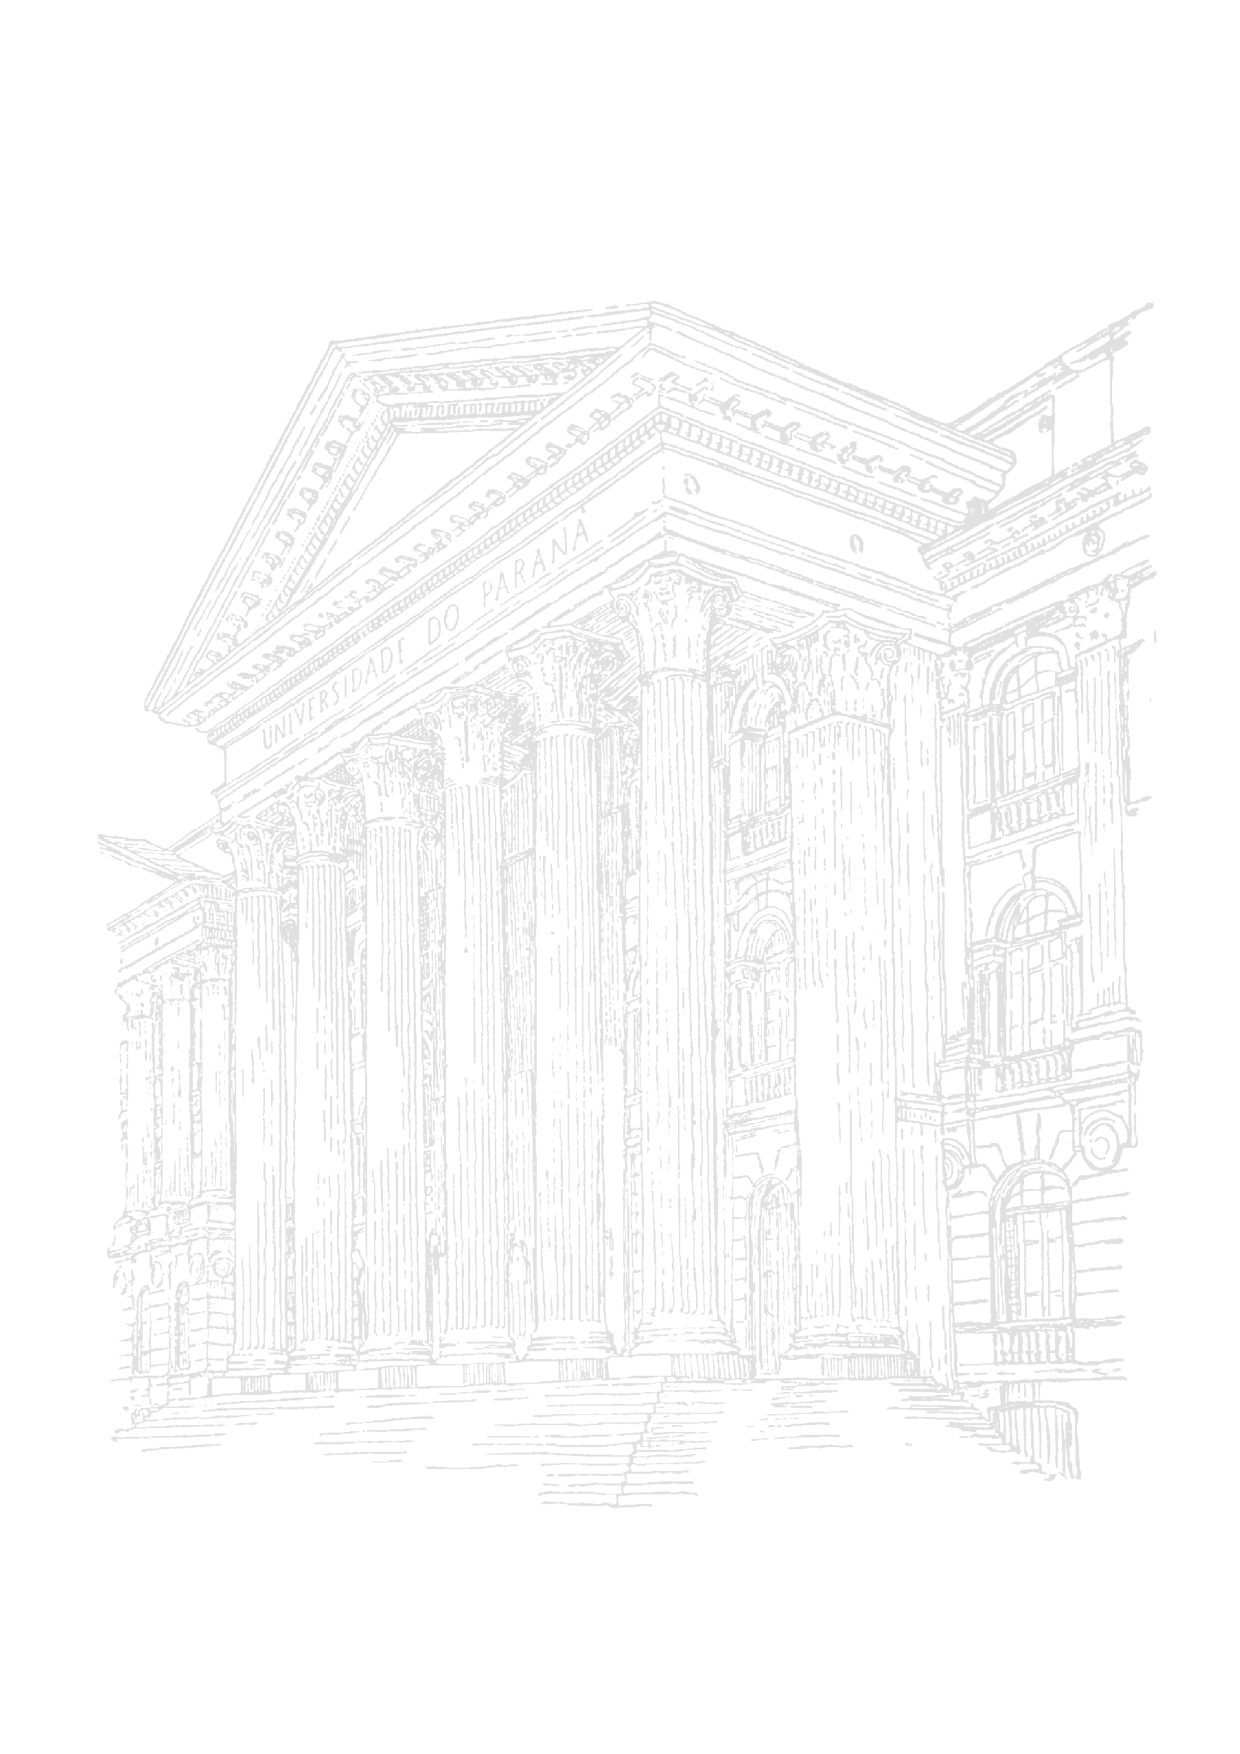
\includegraphics[width=\paperwidth,
  height=\paperheight]{Figuras/ufpr_bg}};
% ----------------------------------------------------------------------
\imprimircapa
% ----------------------------------------------------------------------
% folha de rosto
\imprimirfolhaderosto
% ----------------------------------------------------------------------
% \begin{dedicatoria}
%   \vspace*{\fill}
%   ...
%   \vspace*{\fill}
% \end{dedicatoria}
% ----------------------------------------------------------------------
% ficha catalográfica

% \begin{fichacatalografica}
%   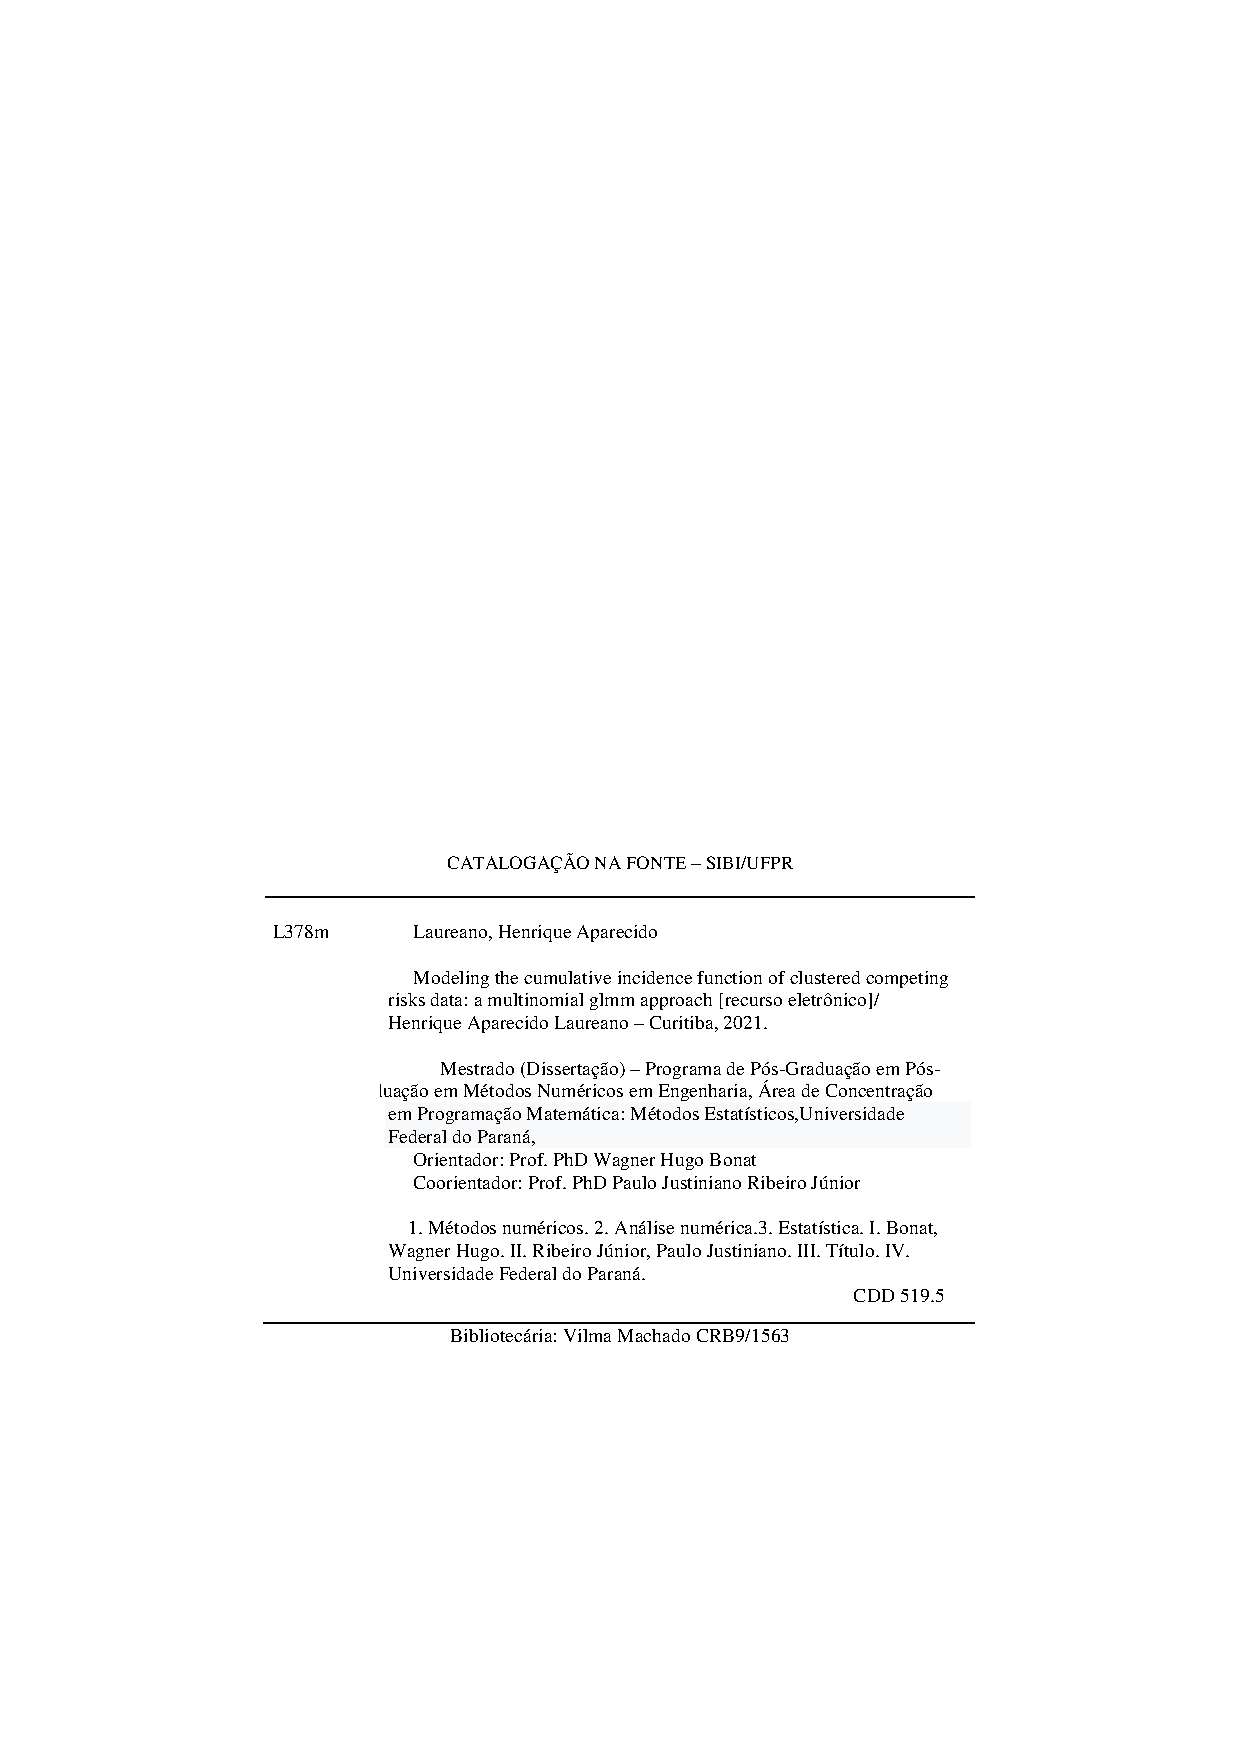
\includepdf{ficha.pdf}
% \end{fichacatalografica}
% ----------------------------------------------------------------------
% inserir folha de aprovação
% \begin{folhadeaprovacao}
%   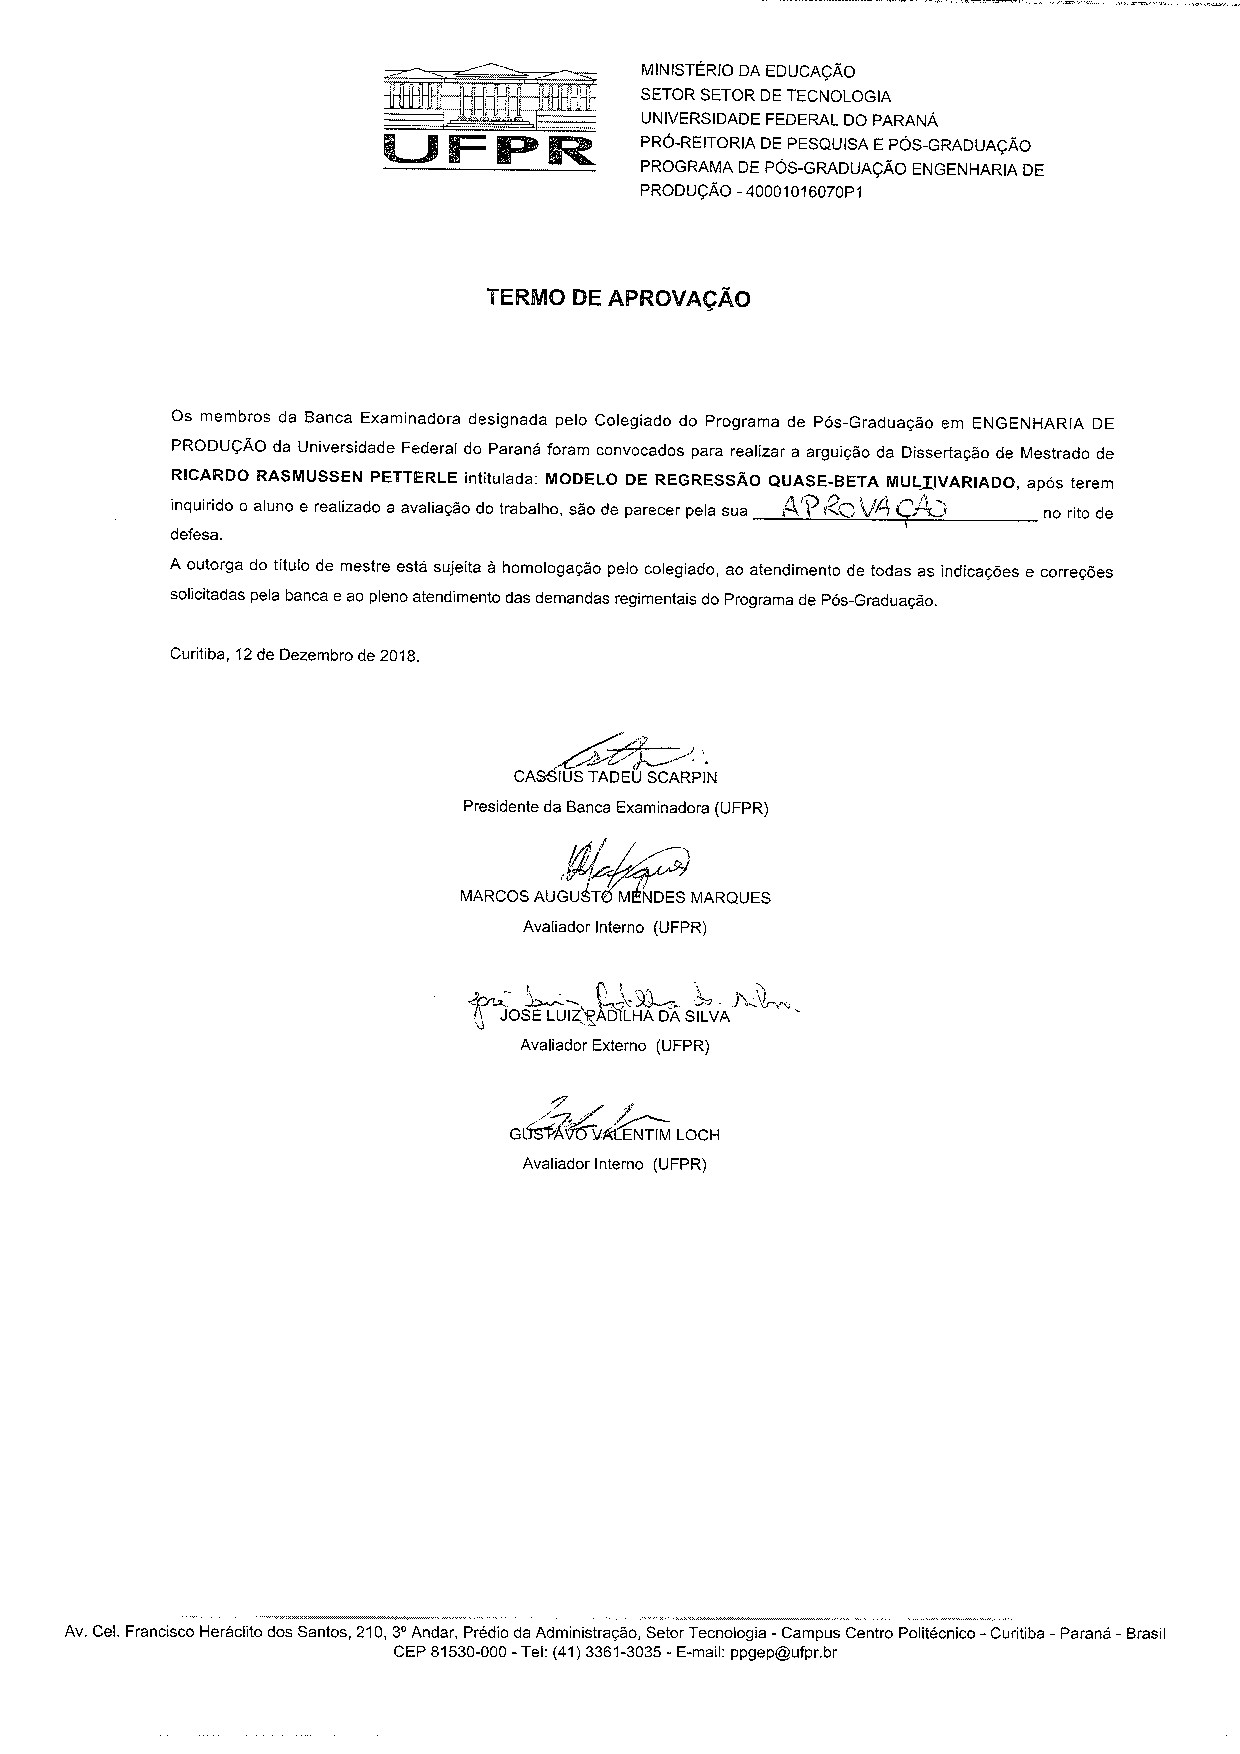
\includepdf{termo.pdf}
% \end{folhadeaprovacao}
\begin{folhadeaprovacao}
 \begin{center}
   {\ABNTEXchapterfont\large\imprimirautor}

   \vspace*{\fill}\vspace*{\fill}
   \begin{center}
     \ABNTEXchapterfont\bfseries\large\imprimirtitulo
   \end{center}
   \vspace*{\fill}

    \hspace{.45\textwidth}
    \begin{minipage}{.5\textwidth}
       \imprimirpreambulo
    \end{minipage}
   \vspace*{\fill}
 \end{center}

 Master thesis approved. XXX XX, 2021.

  \assinatura{\textbf{\imprimirorientador}\\ Supervisor}
  \assinatura{\textbf{Prof. PhD Paulo Justiniano Ribeiro Jr}\\
    Co-supervisor}
  \assinatura{\textbf{Prof. PhD \(\dots\)}\\
    Internal Examinator - PPGMNE}
  \assinatura{\textbf{Prof. PhD \(\dots\)}\\
    Internal Examinator - PPGMNE}
  \assinatura{\textbf{Prof. PhD \(\dots\)}\\External Examiner - }

  \begin{center}
   \vspace*{0.5cm}
   {\large CURITIBA}
   \par
   {\large\imprimirdata}
   \vspace*{1cm}
 \end{center}

\end{folhadeaprovacao}
% ----------------------------------------------------------------------
\begin{dedicatoria}
  \vspace*{22.7cm}
  \begin{flushright}
    \begin{minipage}[H]{4.5cm}
      {To Celita and Olivio}
    \end{minipage}
  \end{flushright}
\end{dedicatoria}
% ----------------------------------------------------------------------
\begin{agradecimentos}
 As Moro once said, I am thankful for everything and everyone.

 Today is the shadow of tomorrow. Today is the present future of
 yesterday. Yesterday is the shadow of today. The wisdom of the past is
 the light of the past. The light of the future casts the shadows of
 tomorrow.
\end{agradecimentos}

\begin{epigrafe}
  \vspace*{\fill}
  \begin{flushright}
    \textit{"It's not supposed to be easy."\\
             (Gregg Popovich)}
              % on Sao Antonio Spurs \(\times\) Oklahoma City Thunder,
              % first game of the 2012 Western Conference Finais
  \end{flushright}
\end{epigrafe}
% ----------------------------------------------------------------------
\newpage
\setlength{\absparsep}{18pt} % ajusta o espaçamento dos parágrafos do
                             % resumo
\setlength{\abstitleskip}{1cm} % adiciona mais um cm após o 'titulo' do
                               % resumo para ficar com 2cm
\begin{resumo}[]
  \vspace{-2cm}
  \begin{center}
    \bfseries{\large{\textsf{ABSTRACT}}}
  \end{center}
  \vspace{0.3cm}

  Clustered competing risks data is a special case of failure time
  data. Besides the cluster structure which implies a within-cluster
  dependence between its elements, this kind of data is characterized by
  1) multiple causes/variables competing to be the one responsible for
  the occurrence of an event, a failure; and 2) censorship, when the
  event of interest happens for none of the competing causes, in the
  study period.

  To handle this type of data, we propose a latent-effects framework, a
  generalized linear mixed model (GLMM), instead of a usual survival
  model. In survival analysis, the modeling is done by means of the
  hazard rate, and the within-cluster dependence accommodation generates
  a complicated likelihood function sometimes intractable. What we do
  here is to model the clustered competing causes in the probability
  scale, in terms of the cumulative incidence function (CIF) of each
  competing cause. In our framework, we suppose a multinomial
  probability distribution for the competing causes and censorship,
  conditioned on the latent effects (within-cluster dependence). The
  latent effects are accommodated by a multivariate Gaussian
  distribution and are modeled by the parameters of its covariance
  matrix. These probability distributions are connected by the CIF,
  modeled here following the specification in \citeonline{SCHEIKE},
  based on the CIF decomposition as the product of an instantaneous risk
  level function with a trajectory time level function. The latent
  effects are inserted in those level functions.  To make the estimation
  of the parameters of this model the most efficient as possible, we use
  the template model builder (TMB) \cite{TMB}. With this R \cite{R21}
  package, we have our log-likelihood function written in C++, we have
  access to state-of-the-art computational libraries, an efficient
  Laplace approximation implementation for the latent-effects, and an
  automatic differentiation (AD) routine, the state-of-the-art in
  derivatives computation. To check the estimability of our model a
  large simulation study is performed, based on different latent
  structure formulations, with the aim to verify which one is most
  adequate. The model presents to be of difficult estimation, with our
  results converging to a latent restructure where the risk and
  trajectory time levels are correlated. In scenarios with high CIF the
  model exhibits good results, but with an excessive variance, showing
  that improvements are necessary.
  
  In scenarios with high CIF the model exhibits good results, but with
  an excessive variance, showing that improvements are necessary.
  
  \textbf{Keywords}: Clustered competing risks.
                     Within-cluster dependence.
                     Multinomial generalized linear mixed model (GLMM).
                     TMB: Template Model Builder.
                     Laplace approximation.
                     Automatic differentiation (AD).
\end{resumo}
% ----------------------------------------------------------------------
\newpage
\setlength{\absparsep}{18pt} % ajusta o espaçamento dos parágrafos do
                             % resumo
\setlength{\abstitleskip}{1cm} % adiciona mais um cm após o 'titulo' do
                               % resumo para ficar com 2cm
\begin{resumo}[]
  \begin{otherlanguage*}{brazil}
    \vspace{-2cm}
    \begin{center}
      \bfseries{\large{\textsf{RESUMO}}}
    \end{center}
    \vspace{0.3cm}

    \textbf{Palavras-chave}: Riscos competitivos agrupados.
                             Depend\^{e}ncia intra-cluster.
                             Modelo linear generalizado misto
                             multinomial (MLGM).
                             TMB: Template Model Builder.
                             Aproxima\c{c}\~{a}o de Laplace.
                             Diferencia\c{c}\~{a}o autom\'{a}tica.
  \end{otherlanguage*}
\end{resumo}
% ----------------------------------------------------------------------
\pdfbookmark[0]{\listfigurename}{lof}
\listoffigures*
\cleardoublepage
% ----------------------------------------------------------------------
%% \pdfbookmark[0]{\listtablename}{lot}
%% \listoftables*
%% \cleardoublepage
% ----------------------------------------------------------------------
\makeatletter
\renewcommand\numberline[1]{
	\leftskip -0.7em
	\rightskip 1.6em
	\parfillskip -\rightskip
	\parindent 0em
	\@tempdima 2.0em
	\vspace{0em}
  \advance\leftskip \@tempdima \null\nobreak\hskip -\leftskip
	ALGORITHM \normalfont #1 ~~ }
\makeatother
% ----------------------------------------------------------------------
\pdfbookmark[0]{\listalgorithmname}{loa}
\listofalgorithms
\cleardoublepage
% ----------------------------------------------------------------------
\makeatletter
\def\numberline#1{\hb@xt@\@tempdima{#1\hfil}}
\makeatother
% ----------------------------------------------------------------------
% \begin{siglas}
% \item[Fig.] Area of the $i^{th}$ component
% \item[456] Isto é um número
% \item[123] Isto é outro número
% \item[lauro cesar] este é o meu nome
% \end{siglas}
% ----------------------------------------------------------------------
% \begin{simbolos}
% \item[\(\mathbb{E}(\cdot)\)] The mathematical expectation of a random
%   variable \(\cdot\)
% \end{simbolos}
% ----------------------------------------------------------------------
\pdfbookmark[0]{\contentsname}{toc}
\tableofcontents*
\cleardoublepage
% ----------------------------------------------------------------------
\makepagestyle{abntheadings}
\makeevenhead{abntheadings}{\ABNTEXfontereduzida\thepage}{}{}
\makeoddhead{abntheadings}{}{}{\ABNTEXfontereduzida\thepage}
\makeheadrule{abntheadings}{\textwidth}{0in}
% ----------------------------------------------------------------------
\textual
% ----------------------------------------------------------------------
\chapter{Introduction}
\label{cap:intro}
\input{./modules/intro}
% ----------------------------------------------------------------------
\chapter{Generalized linear mixed models: formulation, optimization, and
  implementation}
\label{cap:methods}
\input{./modules/methods}
% ----------------------------------------------------------------------
\chapter{\(\text{multiGLMM}\): a multinomial GLMM for clustered
  competing risks data}
\label{cap:model}
\input{./modules/model}
% ----------------------------------------------------------------------
\chapter{simulation study datasets}
\label{cap:datasets}
\input{./modules/datasets}
% ----------------------------------------------------------------------
\chapter{Results}
\label{cap:results}
\input{./modules/results}
% ----------------------------------------------------------------------
\chapter{Final considerations}
\label{cap:finalc}
\input{./modules/finalc}
% ----------------------------------------------------------------------
\setlength{\afterchapskip}{\baselineskip}
% ----------------------------------------------------------------------
\bibliography{references}
% ----------------------------------------------------------------------
\postextual
% ----------------------------------------------------------------------
\begin{apendicesenv}
\partapendices
\addcontentsline{toc}{chapter}{\hspace{2.105cm}APPENDIX}
\renewcommand{\ABNTEXchapterfontsize}{\ABNTEXsectionfont}

\chapter{ANALYTIC GRADIENT OF THE LATENT EFFECTS FOR THE JOINT
         LOG-LIKELIHOOD FUNCTION OF THE MULTINOMIAL GLMM FOR CLUSTERED
         COMPETING RISKS DATA}
\label{cap:appendixA}

The following gradient components are computed by cluster, to be used
e.g., in a Newton optimization. Subject \(i\) at cluster \(j\) and for
competing cause \(k\)

\begin{align*}
  &\frac{\partial}{\partial u_{kj}}
    \log L(\bm{\theta}\mid\bm{y}_{j}, \bm{r}_{j}) =\\
  &y_{kij}\frac{1 +
    \sum_{m \neq k}^{K-1}\exp\{\bm{x}_{mij}\bm{\beta}_{mj} + u_{mj}\}
    }{1 +
    \sum_{n = 1}^{K-1}\exp\{\bm{x}_{nij}\bm{\beta}_{nj} + u_{nj}\}} -
    \left(\sum_{m \neq k}^{K-1} y_{mij}\right)
    \frac{\exp\{\bm{x}_{kij}\bm{\beta}_{kj} + u_{kj}\}
    }{1 +
    \sum_{n = 1}^{K-1}\exp\{\bm{x}_{nij}\bm{\beta}_{nj} + u_{nj}\}}-\\
  &y_{Kij}\frac{1}{1 +
    \sum_{n = 1}^{K-1}\exp\{\bm{x}_{nij}\bm{\beta}_{nj} + u_{nj}\}
    }\Bigg(\\
  &\frac{\exp\{\bm{x}_{kij}\bm{\beta}_{kj} + u_{kj}\}
    \left(1 +
    \sum_{m \neq k}^{K-1}\exp\{\bm{x}_{mij}\bm{\beta}_{mj} + u_{mj}\}
    \right)}{
    1 + \sum_{n = 1}^{K-1}\exp\{\bm{x}_{nij}\bm{\beta}_{nj} + u_{nj}\}
    }\times\\
  &\frac{w_{k}\frac{\delta}{2\delta t - 2t^{2}}
    \phi[w_{k}\text{arctanh}\left(\frac{t-\delta/2}{\delta/2}\right)
    - \bm{x}_{kij}\bm{\gamma}_{kj} - \eta_{kj}
    ]}{1 - w_{n}\frac{\delta}{2\delta t - 2t^{2}}
    \phi[w_{n}\text{arctanh}\left(\frac{t-\delta/2}{\delta/2}\right)
    - \bm{x}_{nij}\bm{\gamma}_{nj} - \eta_{nj}]} -
    \frac{\exp\{\bm{x}_{kij}\bm{\beta}_{kj} + u_{kj}\}}{
    1 + \sum_{n = 1}^{K-1}\exp\{\bm{x}_{nij}\bm{\beta}_{nj} + u_{nj}\}}
    \times\\
  &\frac{
    \sum_{m \neq k}^{K-1}
    w_{m}\frac{\delta}{2\delta t - 2t^{2}}
    \phi[w_{m}\text{arctanh}\left(\frac{t-\delta/2}{\delta/2}\right)
    - \bm{x}_{mij}\bm{\gamma}_{mj} - \eta_{mj}]
    \exp\{\bm{x}_{mij}\bm{\beta}_{mj} + u_{mj}\}}{
    1 - w_{n}\frac{\delta}{2\delta t - 2t^{2}}
    \phi[w_{n}\text{arctanh}\left(\frac{t-\delta/2}{\delta/2}\right)
    - \bm{x}_{nij}\bm{\gamma}_{nj} - \eta_{nj}]}\Bigg) -\\
  &\bm{e_{k}^{\top}Qr_{j}},\\
  %% -------------------------------------------------------------------
  \\
  %% -------------------------------------------------------------------
  &\frac{\partial}{\partial \eta_{kj}}
  \log L(\bm{\theta}\mid\bm{y}_{j}, \bm{r}_{j}) =\\
  &y_{kij} (w_{k}\text{arctanh}\left(\frac{t-\delta/2}{\delta/2}\right)
    - \bm{x}_{kij}\bm{\gamma}_{kj} - \eta_{kj}) -\\
  &y_{Kij}\frac{\exp\{\bm{x}_{kij}\bm{\beta}_{kj} + u_{kj}\}
    }{1 + \sum_{n = 1}^{K-1}\exp\{\bm{x}_{nij}\bm{\beta}_{nj} + u_{nj}\}}
    \times\\
  &\frac{
    w_{k}\frac{\delta}{2\delta t - 2t^{2}}
    (w_{k}\text{arctanh}\left(\frac{t-\delta/2}{\delta/2}\right)
    - \bm{x}_{kij}\bm{\gamma}_{kj} - \eta_{kj})
    \phi[w_{k} \text{arctanh}\left(\frac{t-\delta/2}{\delta/2}\right)
    - \bm{x}_{kij}\bm{\gamma}_{kj} - \eta_{kj}
    ]}{1 -
    \sum_{n = 1}^{K-1}
    \frac{\exp\{\bm{x}_{nij}\bm{\beta}_{nj} + u_{nj}\}}{1 +
    \sum_{n = 1}^{K-1}\exp\{\bm{x}_{nij}\bm{\beta}_{nj} + u_{nj}\}}
    w_{n}\frac{\delta}{2\delta t - 2t^{2}}
    \phi[w_{n}\text{arctanh}\left(\frac{t-\delta/2}{\delta/2}\right)
    - \bm{x}_{nij}\bm{\gamma}_{nj} - \eta_{nj}]} -\\
  &\bm{e_{k}^{\top}Qr_{j}},
\end{align*}
with \(\bm{e_{k}^{\top}}\) begin a vector with \(1\) at the \(k\)-th
position and zero elsewhere.

\chapter{ANALYTIC HESSIAN OF THE LATENT EFFECTS FOR THE JOINT
         LOG-LIKELIHOOD FUNCTION OF THE MULTINOMIAL GLMM FOR CLUSTERED
         COMPETING RISKS DATA}
\label{cap:appendixB}

The following hessian components are computed by cluster, to be used
e.g., in a Newton optimization. Subject \(i\) at cluster \(j\) and for
competing cause \(k\)
\begin{align*}
  &\frac{\partial^{2}}{\partial u_{kj}^{2}}
    \log L(\bm{\theta}\mid\bm{y}_{j}, \bm{r}_{j}) =\\
  &-\frac{\left(\sum_{k = 1}^{K-1} y_{kij}\right)
    \exp\{\bm{x}_{kij}\bm{\beta}_{kj} + u_{kj}\}
    \left(1 +
    \sum_{m \neq k}^{K-1}\exp\{\bm{x}_{mij}\bm{\beta}_{mj} + u_{mj}\}
    \right)}{\left(1 +
    \sum_{n = 1}^{K-1}\exp\{\bm{x}_{nij}\bm{\beta}_{nj} + u_{nj}\}
    \right)^{2}} +\\
  &\frac{y_{Kij}
    \exp\{\bm{x}_{kij} \bm{\beta}_{kj} + u_{kj}\}}{
    1 + \sum_{n = 1}^{K-1}\exp\{\bm{x}_{nij} \bm{\beta}_{nj} + u_{nj}\}
    }\times\\
  &\frac{
    \sum_{m \neq k}^{K-1}w_{m}\frac{\delta}{2\delta t - 2t^{2}}
    \phi[w_{m}\text{arctanh}\left(\frac{t-\delta/2}{\delta/2}\right)
    - \bm{x}_{mij}\bm{\gamma}_{mj} - \eta_{mj}]
    \exp\{\bm{x}_{mij}\bm{\beta}_{mj} + u_{mj}\}}{1 +
    \sum_{n = 1}^{K-1}\exp\{\bm{x}_{nij}\bm{\beta}_{nj} + u_{nj}\}
    (1 - w_{n}\frac{\delta}{2\delta t - 2t^{2}}
    \phi[w_{n}\text{arctanh}\left(\frac{t-\delta/2}{\delta/2}\right)
    - \bm{x}_{nij}\bm{\gamma}_{nj} - \eta_{nj}])} -\\
  &\frac{
    y_{Kij}
    w_{k}\frac{\delta}{2\delta t - 2t^{2}}
    \phi[w_{k}\text{arctanh}\left(\frac{t-\delta/2}{\delta/2}\right)
    - \bm{x}_{kij}\bm{\gamma}_{kj} - \eta_{kj}] }{1 +
    \sum_{n = 1}^{K-1}\exp\{\bm{x}_{nij}\bm{\beta}_{nj} + u_{nj}\}
    }\times\\
  &\frac{\exp\{\bm{x}_{kij}\bm{\beta}_{kj} + u_{kj}\}
    \left(1 +
    \sum_{m \neq k}^{K-1}\exp\{\bm{x}_{mij}\bm{\beta}_{mj} + u_{mj}\}
    \right)}{1 +
    \sum_{n = 1}^{K-1}\exp\{\bm{x}_{nij}\bm{\beta}_{nj} + u_{nj}\}
    (1 - w_{n}\frac{\delta}{2\delta t - 2t^{2}}
    \phi[w_{n}\text{arctanh}\left(\frac{t-\delta/2}{\delta/2}\right)
    - \bm{x}_{nij}\bm{\gamma}_{nj} - \eta_{nj}])} -\\
  &\frac{y_{Kij}\exp\{\bm{x}_{kij}\bm{\beta}_{kj} + u_{kj}\}}{\left(1 +
    \sum_{n = 1}^{K-1}\exp\{\bm{x}_{nij}\bm{\beta}_{nj} + u_{nj}\}
    \right)^{2}}\Bigg(\\
  &\frac{\sum_{m \neq k}^{K-1}
    w_{m}\frac{\delta}{2\delta t - 2t^{2}}
    \phi[w_{m}\text{arctanh}\left(\frac{t-\delta/2}{\delta/2}\right)
    - \bm{x}_{mij}\bm{\gamma}_{mj} - \eta_{mj}]
    \exp\{\bm{x}_{mij}\bm{\beta}_{mj} + u_{mj}\}}{\left(1 +
    \sum_{n = 1}^{K-1}\exp\{\bm{x}_{nij}\bm{\beta}_{nj} + u_{nj}\}
    (1 - w_{n}\frac{\delta}{2\delta t - 2t^{2}}
    \phi[w_{n}\text{arctanh}\left(\frac{t-\delta/2}{\delta/2}\right)
    - \bm{x}_{nij}\bm{\gamma}_{nj} - \eta_{nj}])\right)^{2}}-\\
  &\frac{w_{k}\frac{\delta}{2\delta t - 2t^{2}}
    \phi[w_{k}\text{arctanh}\left(\frac{t-\delta/2}{\delta/2}\right)
    - \bm{x}_{kij}\bm{\gamma}_{kj} - \eta_{kj}]\left(1 +
    \sum_{m \neq k}^{K-1}\exp\{\bm{x}_{mij}\bm{\beta}_{mj} + u_{mj}\}
    \right)}{\left(1 +
    \sum_{n = 1}^{K-1}\exp\{\bm{x}_{nij}\bm{\beta}_{nj} + u_{nj}\}
    (1 - w_{n}\frac{\delta}{2\delta t - 2t^{2}}
    \phi[w_{n}\text{arctanh}\left(\frac{t-\delta/2}{\delta/2}\right)
    - \bm{x}_{nij}\bm{\gamma}_{nj} - \eta_{nj}])\right)^{2}}\Bigg)\\
  &\times\Bigg(\Big(1 +\\
  &\sum_{n = 1}^{K-1}\exp\{\bm{x}_{nij}\bm{\beta}_{nj} + u_{nj}\}
    (1 - w_{n}\frac{\delta}{2\delta t - 2t^{2}}
    \phi[w_{n}\text{arctanh}\left(\frac{t-\delta/2}{\delta/2}\right)
    - \bm{x}_{nij}\bm{\gamma}_{nj} - \eta_{nj}])\Big) +\\
  &\Big(1 +
    \sum_{n = 1}^{K-1}\exp\{\bm{x}_{nij} \bm{\beta}_{nj} + u_{nj}\}
    \Big)\times\\
  &(1 - w_{k}\frac{\delta}{2\delta t - 2t^{2}}
    \phi[w_{k}\text{arctanh}\left(\frac{t-\delta/2}{\delta/2}\right)
    - \bm{x}_{kij}\bm{\gamma}_{kj} - \eta_{kj}])\Bigg)
    - \bm{e_{k}^{\top}Q},
\end{align*}

\begin{align*}
  &\frac{\partial^{2}}{\partial \eta_{kj}^{2}}
    \log L(\bm{\theta}\mid\bm{y}_{j}, \bm{r}_{j}) =\\
  &- y_{kij} - y_{Kij}
    \frac{\exp\{\bm{x}_{kij} \bm{\beta}_{kj} + u_{kj}\}}{1 +
    \sum_{n = 1}^{K-1}\exp\{\bm{x}_{nij} \bm{\beta}_{nj} + u_{nj}\}}\Bigg(\\
  &w_{k}\frac{\delta}{2\delta t - 2t^{2}}
    \phi[w_{k}\text{arctanh}\left(\frac{t-\delta/2}{\delta/2}\right)
    - \bm{x}_{kij}\bm{\gamma}_{kj} - \eta_{kj}]\times\\
  &\frac{\left(
    w_{k} \text{arctanh}\left(\frac{t-\delta/2}{\delta/2}\right)
    - \bm{x}_{kij}\bm{\gamma}_{kj} - \eta_{kj}
    \right)^{2} - 1}{
    1 - \sum_{n = 1}^{K-1}
    \frac{\exp\{\bm{x}_{nij}\bm{\beta}_{nj} + u_{nj}\}}{1 +
    \sum_{n = 1}^{K-1}\exp\{\bm{x}_{nij} \bm{\beta}_{nj} + u_{nj}\}}
    w_{n}\frac{\delta}{2\delta t - 2t^{2}}
    \phi[w_{n}\text{arctanh}\left(\frac{t-\delta/2}{\delta/2}\right)
    - \bm{x}_{nij}\bm{\gamma}_{nj} - \eta_{nj}]} -\\
  &\frac{\left(
    w_{k}\frac{\delta}{2\delta t - 2t^{2}}
    (w_{k}\text{arctanh}\left(\frac{t-\delta/2}{\delta/2}\right)
    - \bm{x}_{kij}\bm{\gamma}_{kj} - \eta_{kj})
    \phi[w_{k}\text{arctanh}\left(\frac{t-\delta/2}{\delta/2}\right)
    - \bm{x}_{kij}\bm{\gamma}_{kj} - \eta_{kj}]\right)^{2}}{\left(1 -
    \sum_{n = 1}^{K-1}
    \frac{\exp\{\bm{x}_{nij} \bm{\beta}_{nj} + u_{nj}\}}{1 +
    \sum_{n = 1}^{K-1}\exp\{\bm{x}_{nij} \bm{\beta}_{nj} + u_{nj}\}}
    w_{n}\frac{\delta}{2\delta t - 2t^{2}}
    \phi[w_{n}\text{arctanh}\left(\frac{t-\delta/2}{\delta/2}\right)
    - \bm{x}_{nij}\bm{\gamma}_{nj} - \eta_{nj}]\right)^{2}}\\
  &\Bigg) - \bm{e_{k}^{\top}Q},
\end{align*}

\begin{align*}
  &\frac{\partial^{2}}{\partial u_{kj} u_{mj}}
    \log L(\bm{\theta}\mid\bm{y}_{j}, \bm{r}_{j}) =\\
  &\left(\sum_{k = 1}^{K-1} y_{kij}\right)
    \frac{
    \exp\{\bm{x}_{kij}\bm{\beta}_{kj} + u_{kj}\}
    \exp\{\bm{x}_{mij}\bm{\beta}_{mj} + u_{mj}\}}{
    \left(1 +
    \sum_{n = 1}^{K-1}\exp\{\bm{x}_{nij} \bm{\beta}_{nj} + u_{nj}\}
    \right)^{2}} +\\
  &\frac{
    y_{Kij}
    \exp\{\bm{x}_{kij}\bm{\beta}_{kj} + u_{kj}\}
    \exp\{\bm{x}_{mij} \bm{\beta}_{mj} + u_{mj}\}}{1 +
    \sum_{n = 1}^{K-1}\exp\{\bm{x}_{nij} \bm{\beta}_{nj} + u_{nj}\}}\Bigg(\\
  &\frac{
    w_{m}\frac{\delta}{2\delta t - 2t^{2}}
    \phi[w_{m}\text{arctanh}\left(\frac{t-\delta/2}{\delta/2}\right)
    - \bm{x}_{mij}\bm{\gamma}_{mj} - \eta_{mj}]}{1 +
    \sum_{n = 1}^{K-1}\exp\{\bm{x}_{nij} \bm{\beta}_{nj} + u_{nj}\}
    (1 - w_{n}\frac{\delta}{2\delta t - 2t^{2}}
    \phi[w_{n}\text{arctanh}\left(\frac{t-\delta/2}{\delta/2}\right)
    - \bm{x}_{nij}\bm{\gamma}_{nj} - \eta_{nj}])} -\\
  &\frac{
    w_{k}\frac{\delta}{2\delta t - 2t^{2}}
    \phi[w_{k}\text{arctanh}\left(\frac{t-\delta/2}{\delta/2}\right)
    - \bm{x}_{kij}\bm{\gamma}_{kj} - \eta_{kj}]}{1 +
    \sum_{n = 1}^{K-1}\exp\{\bm{x}_{nij}\bm{\beta}_{nj} + u_{nj}\}
    (1 - w_{n}\frac{\delta}{2\delta t - 2t^{2}}
    \phi[w_{n}\text{arctanh}\left(\frac{t-\delta/2}{\delta/2}\right)
    - \bm{x}_{nij}\bm{\gamma}_{nj} - \eta_{nj}])}\Bigg) -\\
  &\frac{y_{Kij}}{
    \left(1 +
    \sum_{n = 1}^{K-1}\exp\{\bm{x}_{nij}\bm{\beta}_{nj} + u_{nj}\}
    \right)^{2}}\Bigg(\exp\{\bm{x}_{kij}\bm{\beta}_{kj} + u_{kj}\}\Bigg(\\
  &\frac{
    \sum_{m \neq k}^{K-1}
    w_{m}\frac{\delta}{2\delta t - 2t^{2}}
    \phi[w_{m}\text{arctanh}\left(\frac{t-\delta/2}{\delta/2}\right)
    - \bm{x}_{mij}\bm{\gamma}_{mj} - \eta_{mj}]
    \exp\{\bm{x}_{mij} \bm{\beta}_{mj} + u_{mj}\}}{
    \left(1 + \sum_{n = 1}^{K-1}\exp\{\bm{x}_{nij}\bm{\beta}_{nj} + u_{nj}\}
    (1 - w_{n}\frac{\delta}{2\delta t - 2t^{2}}
    \phi[w_{n}\text{arctanh}\left(\frac{t-\delta/2}{\delta/2}\right)
    - \bm{x}_{nij}\bm{\gamma}_{nj} - \eta_{nj}])\right)^{2}} -\\
  &\frac{
    w_{k}\frac{\delta}{2\delta t - 2t^{2}}
    \phi[w_{k}\text{arctanh}\left(\frac{t-\delta/2}{\delta/2}\right)
    - \bm{x}_{kij}\bm{\gamma}_{kj} - \eta_{kj}]
    \left(1 +
    \sum_{m \neq k}^{K-1}\exp\{\bm{x}_{mij}\bm{\beta}_{mj} + u_{mj}\}
    \right)}{\left(1 +
    \sum_{n = 1}^{K-1}\exp\{\bm{x}_{nij} \bm{\beta}_{nj} + u_{nj}\}
    (1 - w_{n}\frac{\delta}{2\delta t - 2t^{2}}
    \phi[w_{n}\text{arctanh}\left(\frac{t-\delta/2}{\delta/2}\right)
    - \bm{x}_{nij}\bm{\gamma}_{nj} - \eta_{nj}])\right)^{2}}\Bigg)
\end{align*}
\begin{align*}
  &\Bigg)\times\Bigg(\exp\{\bm{x}_{mij}\bm{\beta}_{mj} + u_{mj}\}
    \Big(1 +\\
  &\sum_{n = 1}^{K-1}\exp\{\bm{x}_{nij}\bm{\beta}_{nj} + u_{nj}\}
    (1 - w_{n}\frac{\delta}{2\delta t - 2t^{2}}
    \phi[w_{n}\text{arctanh}\left(\frac{t-\delta/2}{\delta/2}\right)
    - \bm{x}_{nij}\bm{\gamma}_{nj} - \eta_{nj}])\Big) +\\
  &\exp\{\bm{x}_{mij}\bm{\beta}_{mj} + u_{mj}\}
    (1 - w_{m}\frac{\delta}{2\delta t - 2t^{2}}
    \phi[w_{m}\text{arctanh}\left(\frac{t-\delta/2}{\delta/2}\right)
    - \bm{x}_{mij}\bm{\gamma}_{mj} - \eta_{mj}])\Big(1 +\\
  &\sum_{n = 1}^{K-1}\exp\{\bm{x}_{nij}\bm{\beta}_{nj} + u_{nj}\}\Big)
    \Bigg) - \bm{e_{k}^{\top}Q},
\end{align*}

\begin{align*}
  &\frac{\partial^{2}}{\partial \eta_{kj} \eta_{mj}}
    \log L(\bm{\theta}\mid\bm{y}_{j}, \bm{r}_{j}) =\\
  &- y_{Kij}\frac{
    \exp\{\bm{x}_{kij}\bm{\beta}_{kj} + u_{kj}\}}{1 +
    \sum_{n = 1}^{K-1}\exp\{\bm{x}_{nij}\bm{\beta}_{nj} + u_{nj}\}}\times\\
  &\frac{w_{k}\frac{\delta}{2\delta t - 2t^{2}}
    (w_{k}\text{arctanh}\left(\frac{t-\delta/2}{\delta/2}\right)
    - \bm{x}_{kij}\bm{\gamma}_{kj} - \eta_{kj})
    \phi[w_{k}\text{arctanh}\left(\frac{t-\delta/2}{\delta/2}\right)
    - \bm{x}_{kij}\bm{\gamma}_{kj} - \eta_{kj}]}{\left(1 -
    \sum_{n = 1}^{K-1}\frac{\exp\{\bm{x}_{nij}\bm{\beta}_{nj} + u_{nj}\}
    }{1 +
    \sum_{n = 1}^{K-1}\exp\{\bm{x}_{nij}\bm{\beta}_{nj} + u_{nj}\}}
    w_{n}\frac{\delta}{2\delta t - 2t^{2}}
    \phi[w_{n}\text{arctanh}\left(\frac{t-\delta/2}{\delta/2}\right)
    - \bm{x}_{nij}\bm{\gamma}_{nj} - \eta_{nj}]\right)^{2}}\times\\
  &\frac{\exp\{\bm{x}_{mij}\bm{\beta}_{mj} + u_{mj}\}}{1 +
    \sum_{n = 1}^{K-1}\exp\{\bm{x}_{nij}\bm{\beta}_{nj} + u_{nj}\}}
    w_{m}\frac{\delta}{2\delta t - 2t^{2}}
    (w_{m}\text{arctanh}\left(\frac{t-\delta/2}{\delta/2}\right)
    - \bm{x}_{mij}\bm{\gamma}_{mj} - \eta_{mj})\times\\
  &\phi[w_{m}\text{arctanh}\left(\frac{t-\delta/2}{\delta/2}\right)
    - \bm{x}_{mij}\bm{\gamma}_{mj} - \eta_{mj}] - \bm{e_{k}^{\top}Q},
\end{align*}

\begin{align*}
  &\frac{\partial^{2}}{\partial \eta_{kj} u_{kj}}
    \log L(\bm{\theta}\mid\bm{y}_{j}, \bm{r}_{j}) =\\
  &y_{Kij}
    \frac{\exp\{\bm{x}_{kij}\bm{\beta}_{kj} + u_{kj}\}}{1 +
    \sum_{n = 1}^{K-1}\exp\{\bm{x}_{nij}\bm{\beta}_{nj} + u_{nj}\}}\times\\
  &\frac{
    w_{k}\frac{\delta}{2\delta t - 2t^{2}}
    (w_{k}\text{arctanh}\left(\frac{t-\delta/2}{\delta/2}\right)
    - \bm{x}_{kij}\bm{\gamma}_{kj} - \eta_{kj})
    \phi[w_{k}\text{arctanh}\left(\frac{t-\delta/2}{\delta/2}\right)
    - \bm{x}_{kij}\bm{\gamma}_{kj} - \eta_{kj})]}{
    \left(1 -
    \sum_{n = 1}^{K-1}\frac{\exp\{\bm{x}_{nij}\bm{\beta}_{nj} + u_{nj}\}}{
    1 +
    \sum_{n = 1}^{K-1}\exp\{\bm{x}_{nij}\bm{\beta}_{nj} + u_{nj}\}}
    w_{n}\frac{\delta}{2\delta t - 2t^{2}}
    \phi[w_{n}\text{arctanh}\left(\frac{t-\delta/2}{\delta/2}\right)
    - \bm{x}_{nij}\bm{\gamma}_{nj} - \eta_{nj}]\right)^{2}}\times\\
  &\Bigg(
    \sum_{n \neq k}^{K-1}
    \frac{
    \exp\{\bm{x}_{nij}\bm{\beta}_{nj} + u_{nj}\}
    \exp\{\bm{x}_{kij}\bm{\beta}_{kj} + u_{kj}\}}{
    \left(1 +
    \sum_{n = 1}^{K-1}\exp\{\bm{x}_{nij}\bm{\beta}_{nj} + u_{nj}\}
    \right)^{2}}\times\\
  &w_{n}\frac{\delta}{2\delta t - 2t^{2}}
    \phi[w_{n}\text{arctanh}\left(\frac{t-\delta/2}{\delta/2}\right)
    - \bm{x}_{nij}\bm{\gamma}_{nj} - \eta_{nj}] -\\
  &\frac{\exp\{\bm{x}_{kij}\bm{\beta}_{kj} + u_{kj}\}
    \left(
    \left(1 +
    \sum_{n = 1}^{K-1}\exp\{\bm{x}_{nij}\bm{\beta}_{nj} + u_{nj}\}
    \right) - \exp\{\bm{x}_{kij} \bm{\beta}_{kj} + u_{kj}\}
    \right)}{
    \left(1 +
    \sum_{n = 1}^{K-1}\exp\{\bm{x}_{nij}\bm{\beta}_{nj} + u_{nj}\}
    \right)^{2}}\times\\
  &w_{k}\frac{\delta}{2\delta t - 2t^{2}}
    \phi[w_{k}\text{arctanh}\left(\frac{t-\delta/2}{\delta/2}\right)
    - \bm{x}_{kij}\bm{\gamma}_{kj} - \eta_{kj}]\Bigg) -
\end{align*}
\begin{align*}
  &y_{Kij}
    \frac{
    \frac{\exp\{\bm{x}_{kij}\bm{\beta}_{kj} + u_{kj}\}
    \left(
    \left(1 +
    \sum_{n = 1}^{K-1}\exp\{\bm{x}_{nij}\bm{\beta}_{nj} + u_{nj}\}
    \right) - \exp\{\bm{x}_{kij} \bm{\beta}_{kj} + u_{kj}\}
    \right)}{
    \left(1 +
    \sum_{n = 1}^{K-1}\exp\{\bm{x}_{nij}\bm{\beta}_{nj} + u_{nj}\}
    \right)^{2}}}{1 -
    \sum_{n = 1}^{K-1}\frac{\exp\{\bm{x}_{nij}\bm{\beta}_{nj} + u_{nj}\}}{
    1 + \sum_{n = 1}^{K-1}\exp\{\bm{x}_{nij}\bm{\beta}_{nj} + u_{nj}\}}
    w_{n}\frac{\delta}{2\delta t - 2t^{2}}
    \phi[w_{n}\text{arctanh}\left(\frac{t-\delta/2}{\delta/2}\right)
    - \bm{x}_{nij}\bm{\gamma}_{nj} - \eta_{nj}]}\times\\
  &w_{k}\frac{\delta}{2\delta t - 2t^{2}}
    (w_{k}\text{arctanh}\left(\frac{t-\delta/2}{\delta/2}\right)
    - \bm{x}_{kij}\bm{\gamma}_{kj} - \eta_{kj})\times\\
  &\phi[w_{k}\text{arctanh}\left(\frac{t-\delta/2}{\delta/2}\right)
    - \bm{x}_{kij}\bm{\gamma}_{kj} - \eta_{kj}] - \bm{e_{k}^{\top}Q},
\end{align*}

\begin{align*}
  &\frac{\partial^{2}}{\partial \eta_{kj} u_{mj}}
    \log L(\bm{\theta}\mid\bm{y}_{j}, \bm{r}_{j}) =\\
  &y_{Kij}
    \frac{\exp\{\bm{x}_{kij}\bm{\beta}_{kj} + u_{kj}\}
    \exp\{\bm{x}_{mij}\bm{\beta}_{mj} + u_{mj}\}}{
    \left(1 +
    \sum_{n = 1}^{K-1}\exp\{\bm{x}_{nij}\bm{\beta}_{nj} + u_{nj}\}
    \right)^{2}}\times\\
  &\frac{
    w_{k}\frac{\delta}{2\delta t - 2t^{2}}
    (w_{k} \text{arctanh}\left(\frac{t-\delta/2}{\delta/2}\right)
    - \bm{x}_{kij}\bm{\gamma}_{kj} - \eta_{kj})
    \phi[w_{k}\text{arctanh}\left(\frac{t-\delta/2}{\delta/2}\right)
    - \bm{x}_{kij}\bm{\gamma}_{kj} - \eta_{kj})]}{1 - \sum_{n = 1}^{K-1}
    \frac{\exp\{\bm{x}_{nij}\bm{\beta}_{nj} + u_{nj}\}}{1 +
    \sum_{n = 1}^{K-1}\exp\{\bm{x}_{nij}\bm{\beta}_{nj} + u_{nj}\}}
    w_{n}\frac{\delta}{2\delta t - 2t^{2}}
    \phi[w_{n}\text{arctanh}\left(\frac{t-\delta/2}{\delta/2}\right)
    - \bm{x}_{nij}\bm{\gamma}_{nj} - \eta_{nj}]} +\\
  &y_{Kij}
    \frac{\exp\{\bm{x}_{kij}\bm{\beta}_{kj} + u_{kj}\}}{1 +
    \sum_{n = 1}^{K-1}\exp\{\bm{x}_{nij}\bm{\beta}_{nj} + u_{nj}\}}\times\\
  &\frac{
    w_{k}\frac{\delta}{2\delta t - 2t^{2}}
    (w_{k}\text{arctanh}\left(\frac{t-\delta/2}{\delta/2}\right)
    - \bm{x}_{kij}\bm{\gamma}_{kj} - \eta_{kj})
    \phi[w_{k}\text{arctanh}\left(\frac{t-\delta/2}{\delta/2}\right)
    - \bm{x}_{kij}\bm{\gamma}_{kj} - \eta_{kj})]}{
    \left(1 - \sum_{n = 1}^{K-1}
    \frac{\exp\{\bm{x}_{nij}\bm{\beta}_{nj} + u_{nj}\}}{1 +
    \sum_{n = 1}^{K-1}\exp\{\bm{x}_{nij}\bm{\beta}_{nj} + u_{nj}\}}
    w_{n}\frac{\delta}{2\delta t - 2t^{2}}
    \phi[w_{n}\text{arctanh}\left(\frac{t-\delta/2}{\delta/2}\right)
    - \bm{x}_{nij}\bm{\gamma}_{nj} - \eta_{nj}]\right)^{2}}\times\\
  &\Bigg(
    \sum_{n \neq m}^{K-1}\frac{
    \exp\{\bm{x}_{nij}\bm{\beta}_{nj} + u_{nj}\}
    \exp\{\bm{x}_{mij}\bm{\beta}_{mj} + u_{mj}\}}{
    \left(1 +
    \sum_{n = 1}^{K-1}\exp\{\bm{x}_{nij}\bm{\beta}_{nj} + u_{nj}\}
    \right)^{2}}\times\\
  &w_{n}\frac{\delta}{2\delta t - 2t^{2}}
    \phi[w_{n}\text{arctanh}\left(\frac{t-\delta/2}{\delta/2}\right)
    - \bm{x}_{nij}\bm{\gamma}_{nj} - \eta_{nj}] -\\
  &\frac{\exp\{\bm{x}_{mij}\bm{\beta}_{mj} + u_{mj}\}
    \left(
    \left(1 +
    \sum_{n = 1}^{K-1}\exp\{\bm{x}_{nij}\bm{\beta}_{nj} + u_{nj}\}
    \right) - \exp\{\bm{x}_{mij} \bm{\beta}_{mj} + u_{mj}\}
    \right)}{
    \left(1 + \sum_{n = 1}^{K-1}\exp\{\bm{x}_{nij}\bm{\beta}_{nj} + u_{nj}\}
    \right)^{2}}\times\\
  &w_{m}\frac{\delta}{2\delta t - 2t^{2}}
    \phi[w_{m}\text{arctanh}\left(\frac{t-\delta/2}{\delta/2}\right)
    - \bm{x}_{mij}\bm{\gamma}_{mj} - \eta_{mj}]\Bigg) - \bm{e_{k}^{\top}Q},
\end{align*}
with \(\bm{e_{k}^{\top}}\) begin a vector with \(1\) at the \(k\)-th
position and zero elsewhere.

\chapter{\texttt{R} CODE TO SIMULATE FROM A \(\text{multiGLMM}\) WITH
         TWO COMPETING CAUSES AND CLUSTERS OF SIZE TWO. FOR MORE
         INFORMATION CHECK SECTION \ref{cap:simu}}
\label{cap:appendixC}

\lstinputlisting[firstline=97,lastline=153]{datasets.Rmd}
\vspace{-0.5cm}
\begin{center}
 \begin{footnotesize}
  SOURCE: The author (2021).
 \end{footnotesize}
\end{center}

\chapter{\texttt{C++} CODES FOR THE TMB IMPLEMENTATION OF THE
         \(\text{multiGLMM}\) COMPLETE MODEL'S SPECIAL CASES}
\label{cap:appendixD}

\section{\texttt{C++} CODE FOR THE TMB IMPLEMENTATION OF A
         \(\text{multiGLMM}\) WITH A \(2\times2\) LATENT STRUCTURE ON
         THE RISK LEVEL}
\label{cap:riskModel}

\lstinputlisting[language=C++]{modules/riskModel.cpp}
\vspace{-0.5cm}
\begin{center}
 \begin{footnotesize}
  SOURCE: The author (2021).
 \end{footnotesize}
\end{center}

\section{\texttt{C++} CODE FOR THE TMB IMPLEMENTATION OF A
         \(\text{multiGLMM}\) WITH A \(2\times2\) LATENT STRUCTURE ON
         THE TRAJECTORY TIME LEVEL}
\label{cap:timeModel}

\lstinputlisting[language=C++]{modules/timeModel.cpp}
\vspace{-0.5cm}
\begin{center}
 \begin{footnotesize}
  SOURCE: The author (2021).
 \end{footnotesize}
\end{center}

\section{\texttt{C++} CODE FOR THE TMB IMPLEMENTATION OF A
         \(\text{multiGLMM}\) WITH A BLOCK-DIAG \(4\times4\) LATENT
         STRUCTURE}
\label{cap:blockdiagModel}

\lstinputlisting[language=C++]{modules/blockdiagModel.cpp}
\vspace{-0.5cm}
\begin{center}
 \begin{footnotesize}
  SOURCE: The author (2021).
 \end{footnotesize}
\end{center}

\section{\texttt{R} CODE SHOWING HOW TO LOAD AND FIT THE
         \(\text{multiGLMM}\) VERSIONS}
\label{cap:rscript}

\lstinputlisting{modules/runModel.R}
\vspace{-0.5cm}
\begin{center}
 \begin{footnotesize}
  SOURCE: The author (2021).
 \end{footnotesize}
\end{center}

\chapter{MODEL PARAMETERS BIAS WITH 2.5\% AND 97.5\% QUANTILES}
\label{cap:appendixE}
\vspace{-0.65cm}
\begin{figure}[H]
 \setlength{\abovecaptionskip}{.0001pt}
 \caption{PARAMETER \(\beta_{1}\) BIAS WITH 2.5\% AND 97.5\% QUANTILES}
 \vspace{0.2cm}\centering
 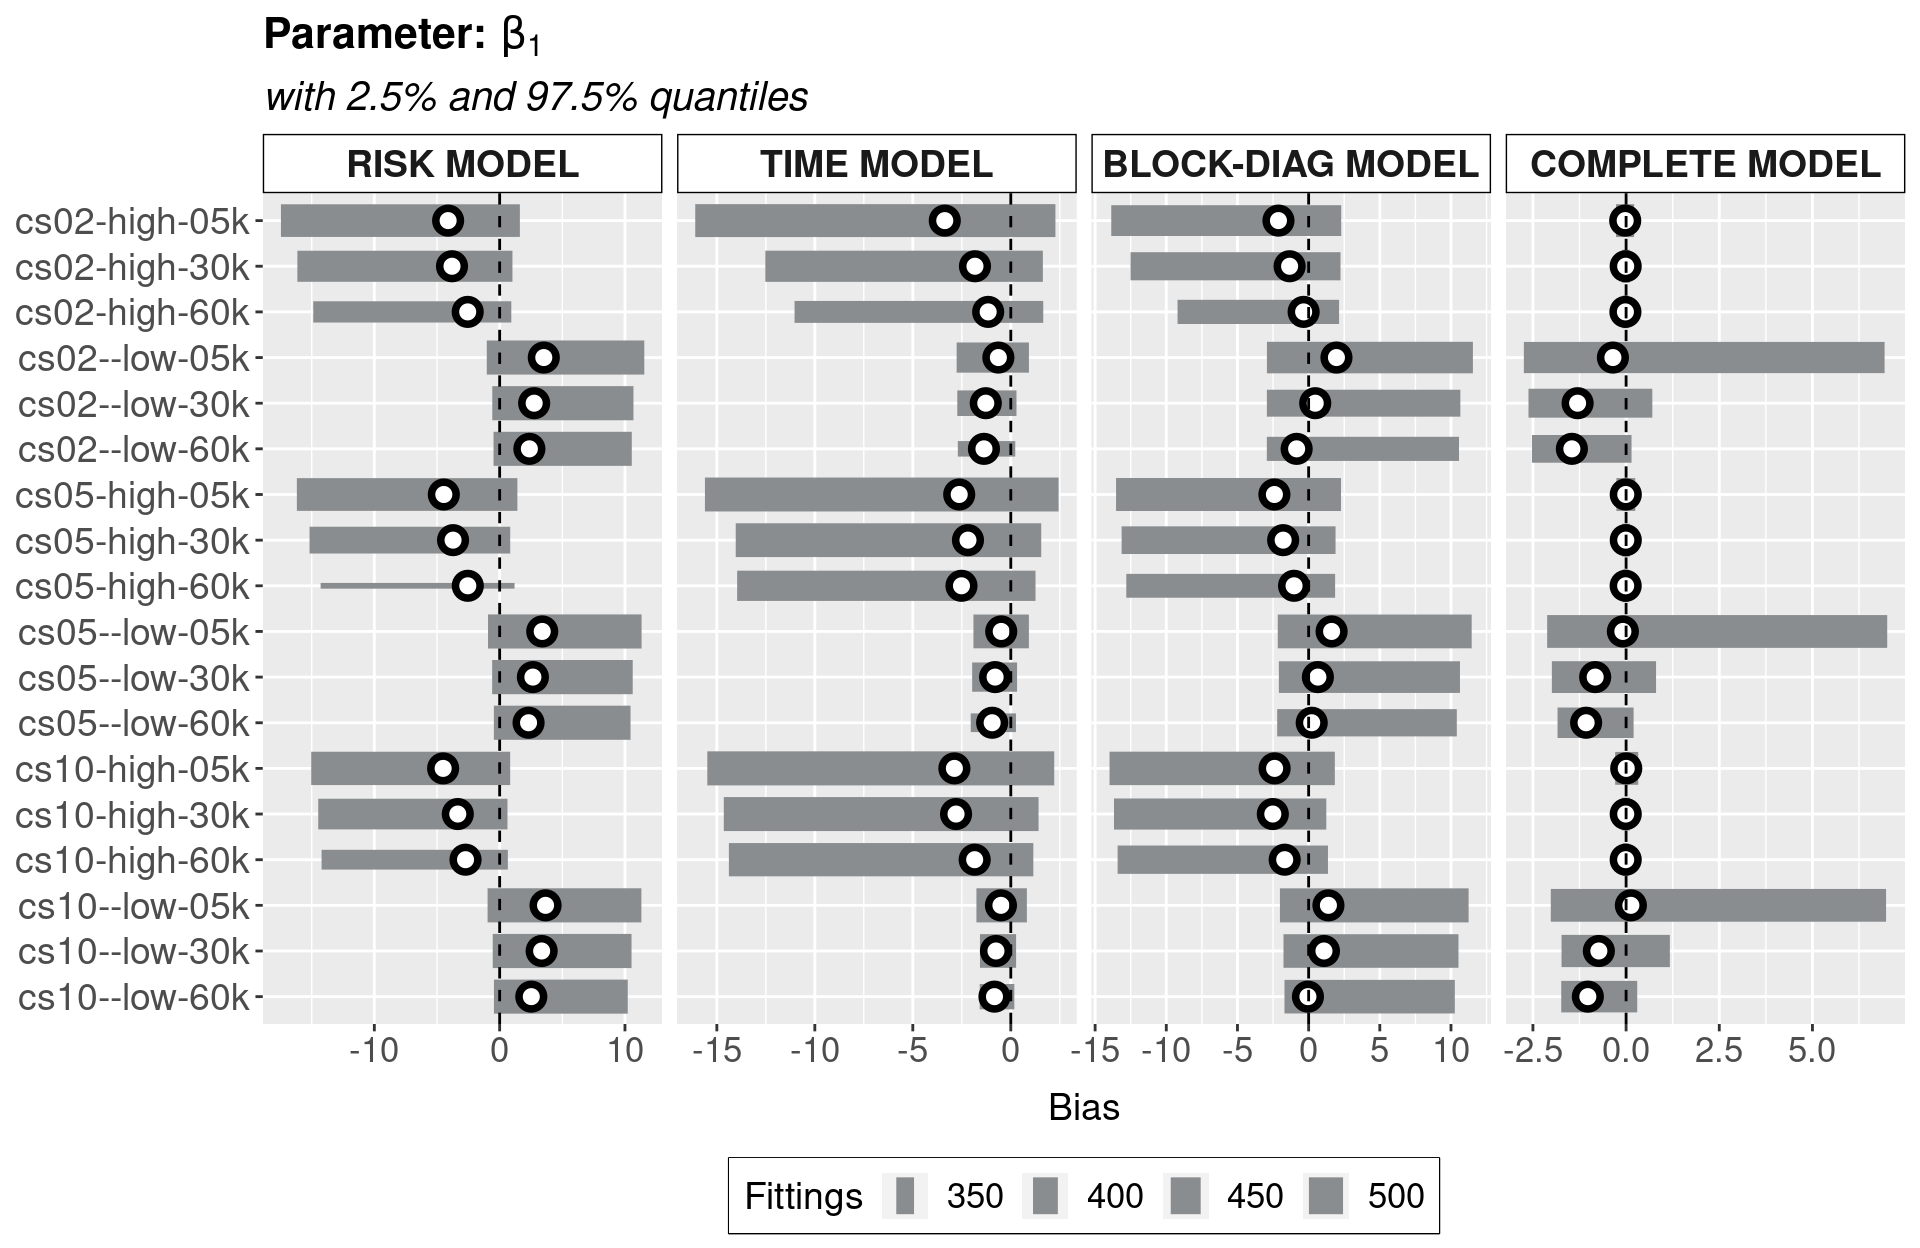
\includegraphics[width=\textwidth]{bias2plot-1.png}\\
 \begin{footnotesize}
  SOURCE: The author (2021).
 \end{footnotesize}
 \label{fig:biasbeta1}
\end{figure}

\begin{figure}[H]
 \setlength{\abovecaptionskip}{.0001pt}
 \caption{PARAMETER \(\beta_{2}\) BIAS WITH 2.5\% AND 97.5\% QUANTILES}
 \vspace{0.2cm}\centering
 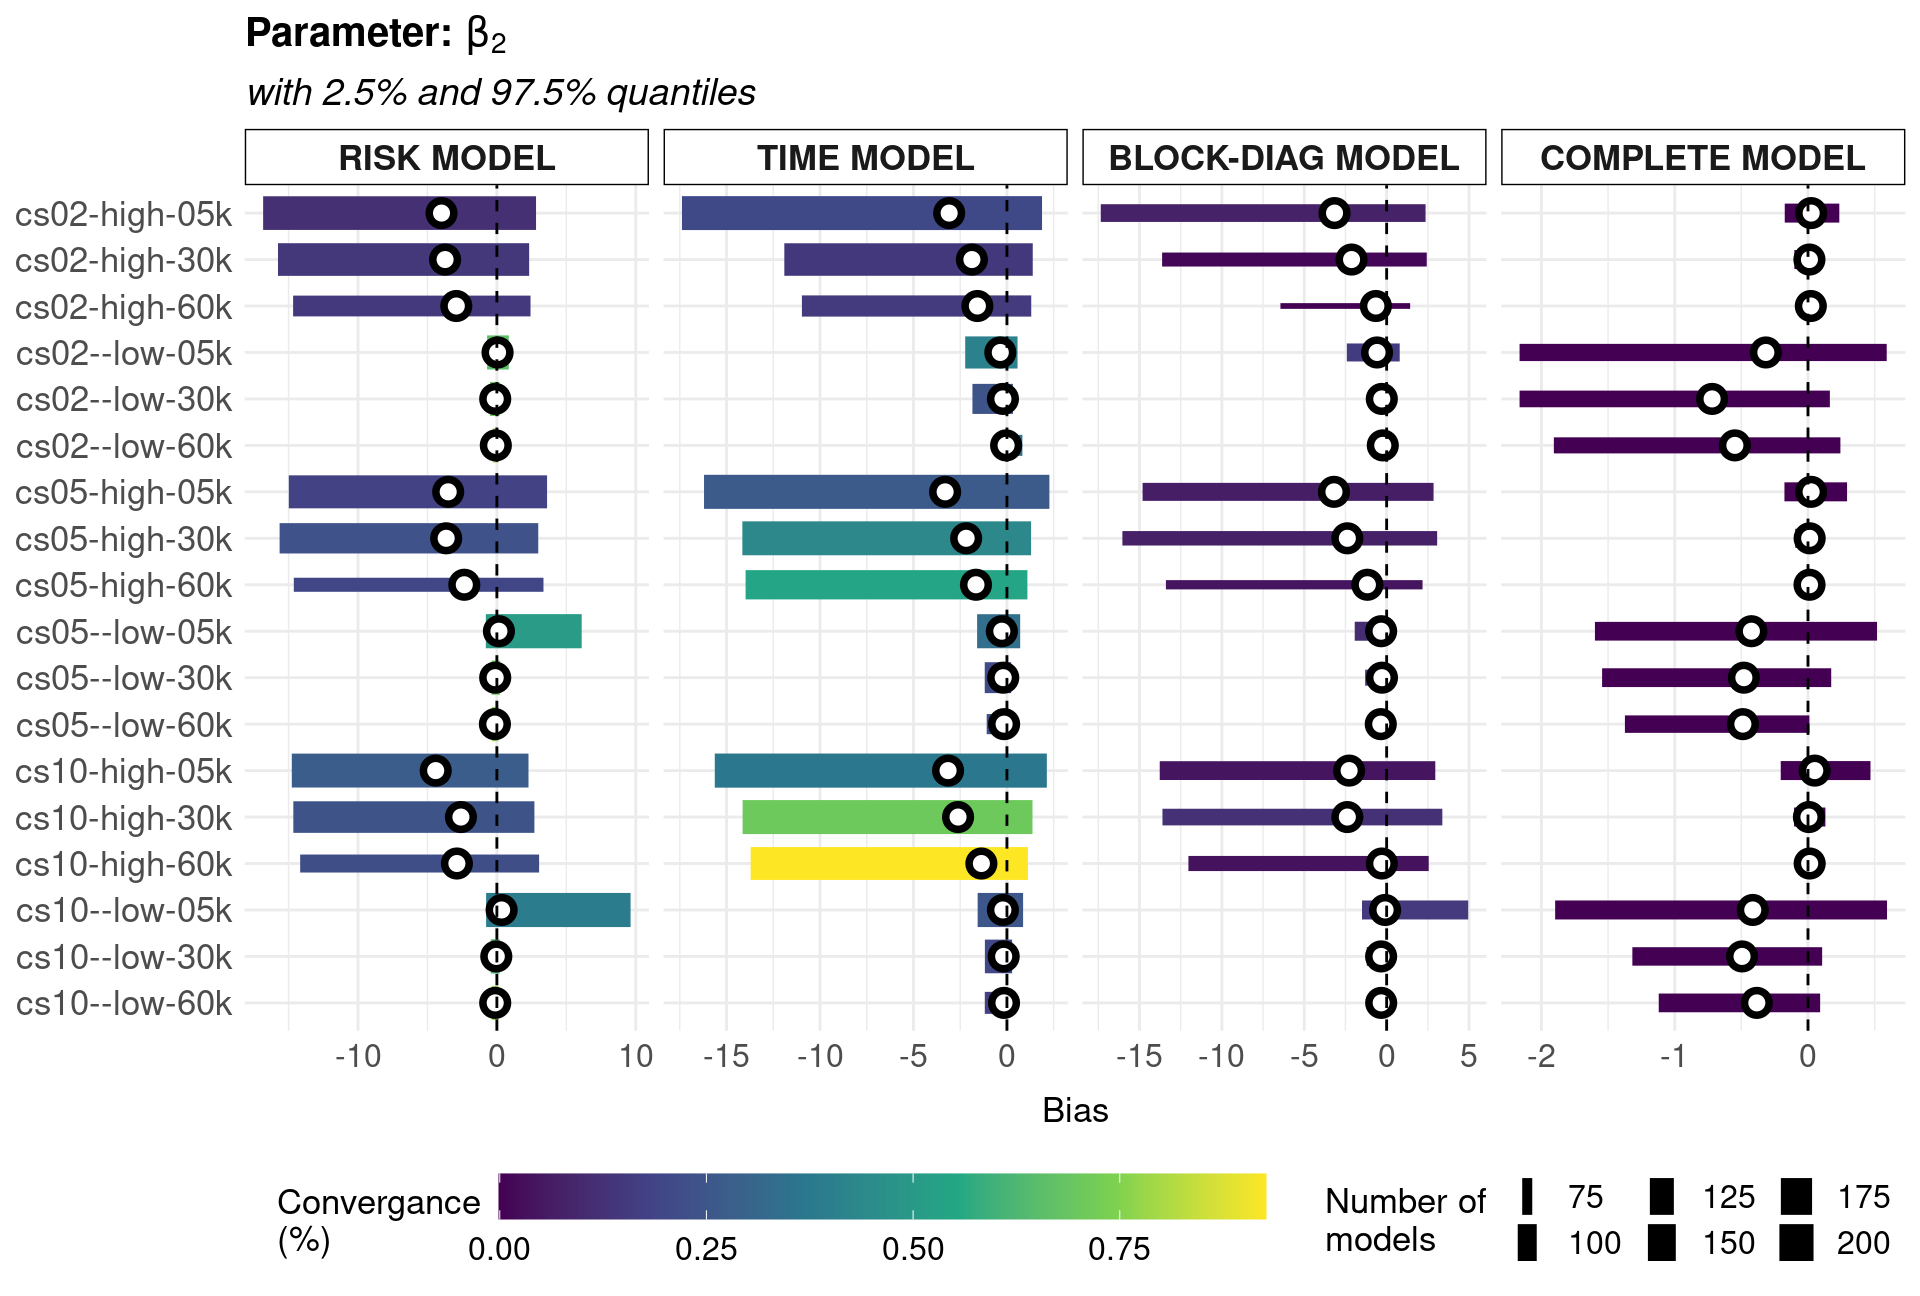
\includegraphics[width=\textwidth]{bias2plot-2.png}\\
 \begin{footnotesize}
  SOURCE: The author (2021).
 \end{footnotesize}
 \label{fig:biasbeta2}
\end{figure}

\begin{figure}[H]
 \setlength{\abovecaptionskip}{.0001pt}
 \caption{PARAMETER \(\gamma_{1}\) BIAS WITH 2.5\% AND 97.5\% QUANTILES}
 \vspace{0.2cm}\centering
 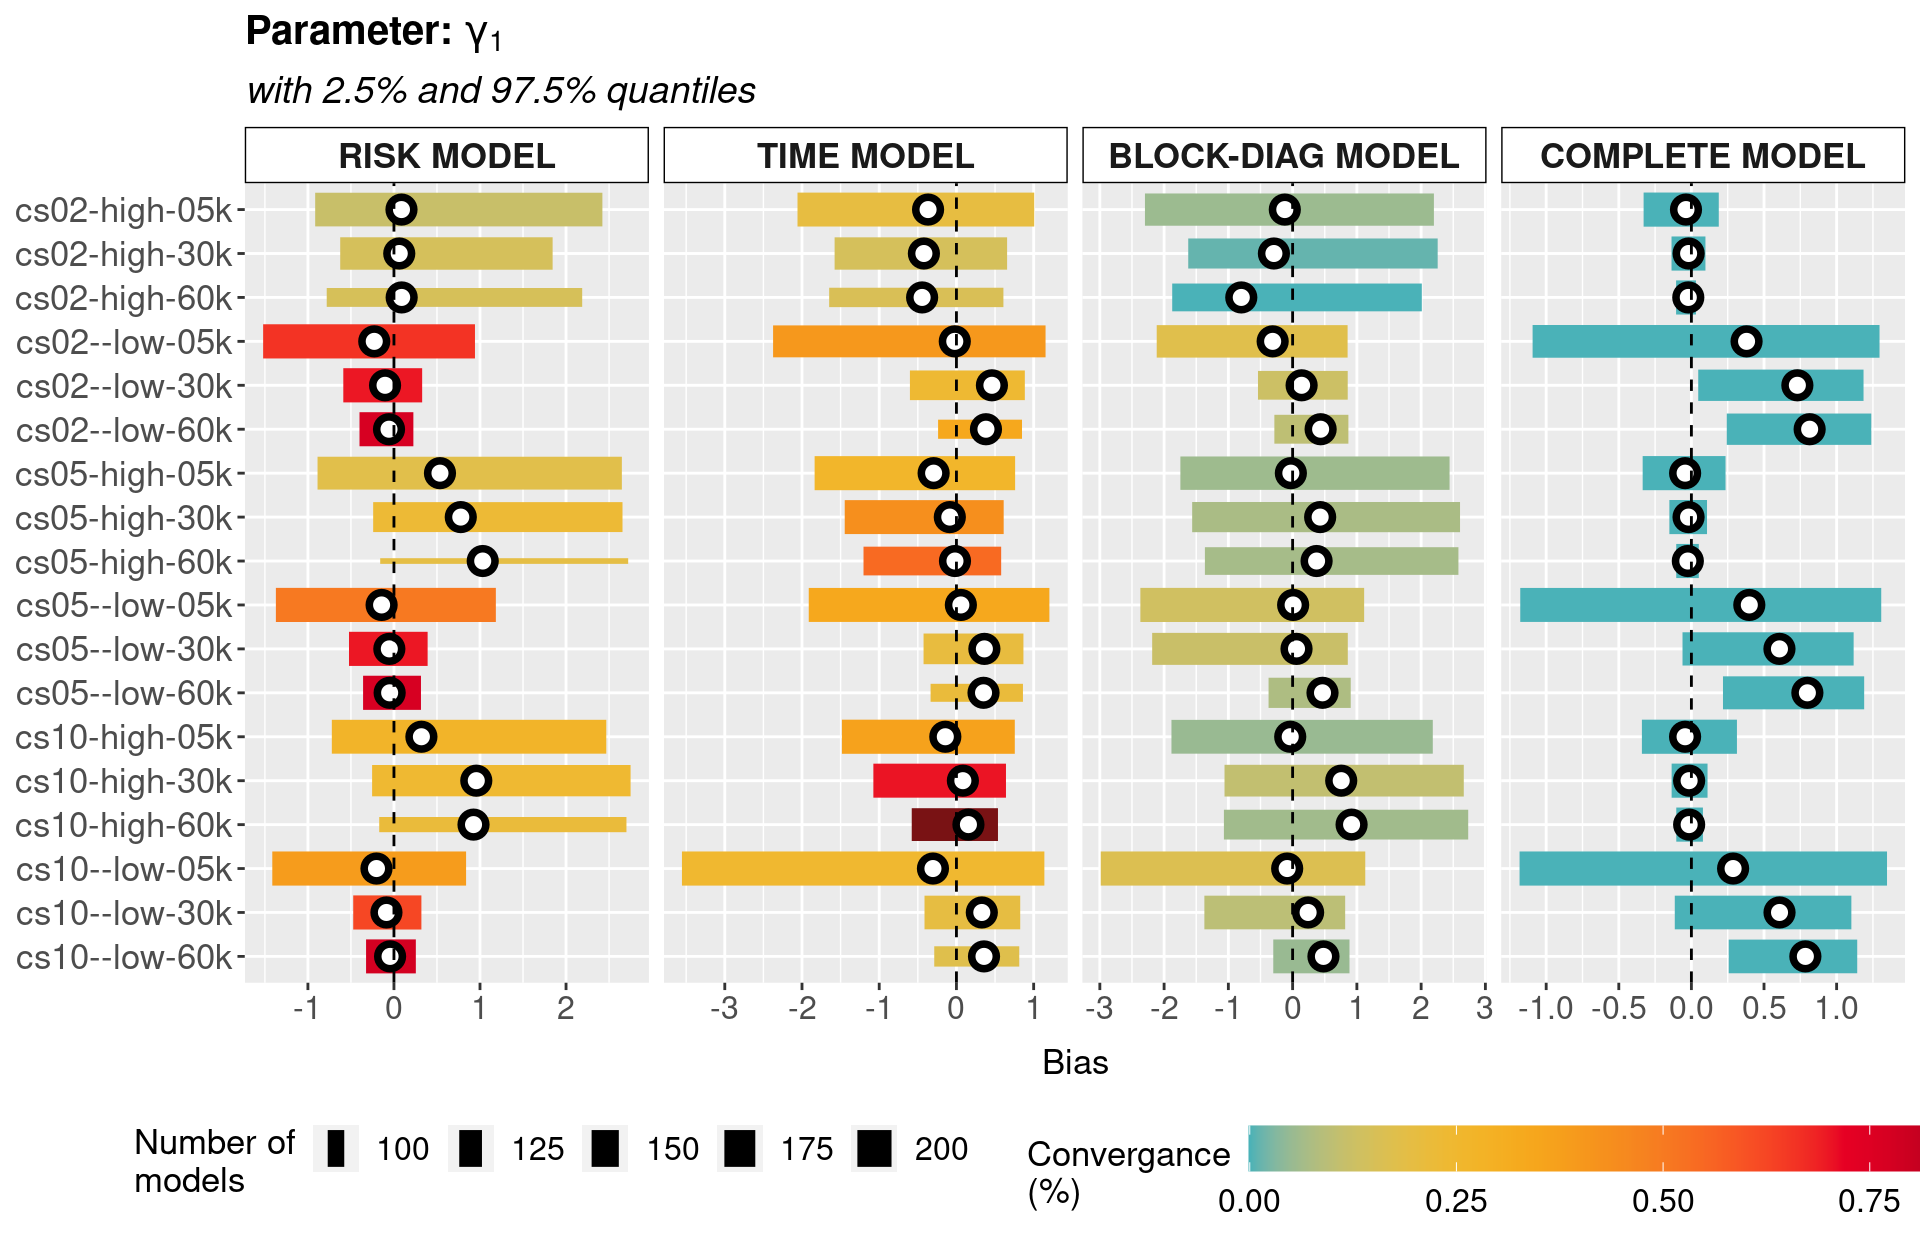
\includegraphics[width=\textwidth]{bias2plot-3.png}\\
 \begin{footnotesize}
  SOURCE: The author (2021).
 \end{footnotesize}
 \label{fig:biasgama1}
\end{figure}

\begin{figure}[H]
 \setlength{\abovecaptionskip}{.0001pt}
 \caption{PARAMETER \(\gamma_{2}\) BIAS WITH 2.5\% AND 97.5\% QUANTILES}
 \vspace{0.2cm}\centering
 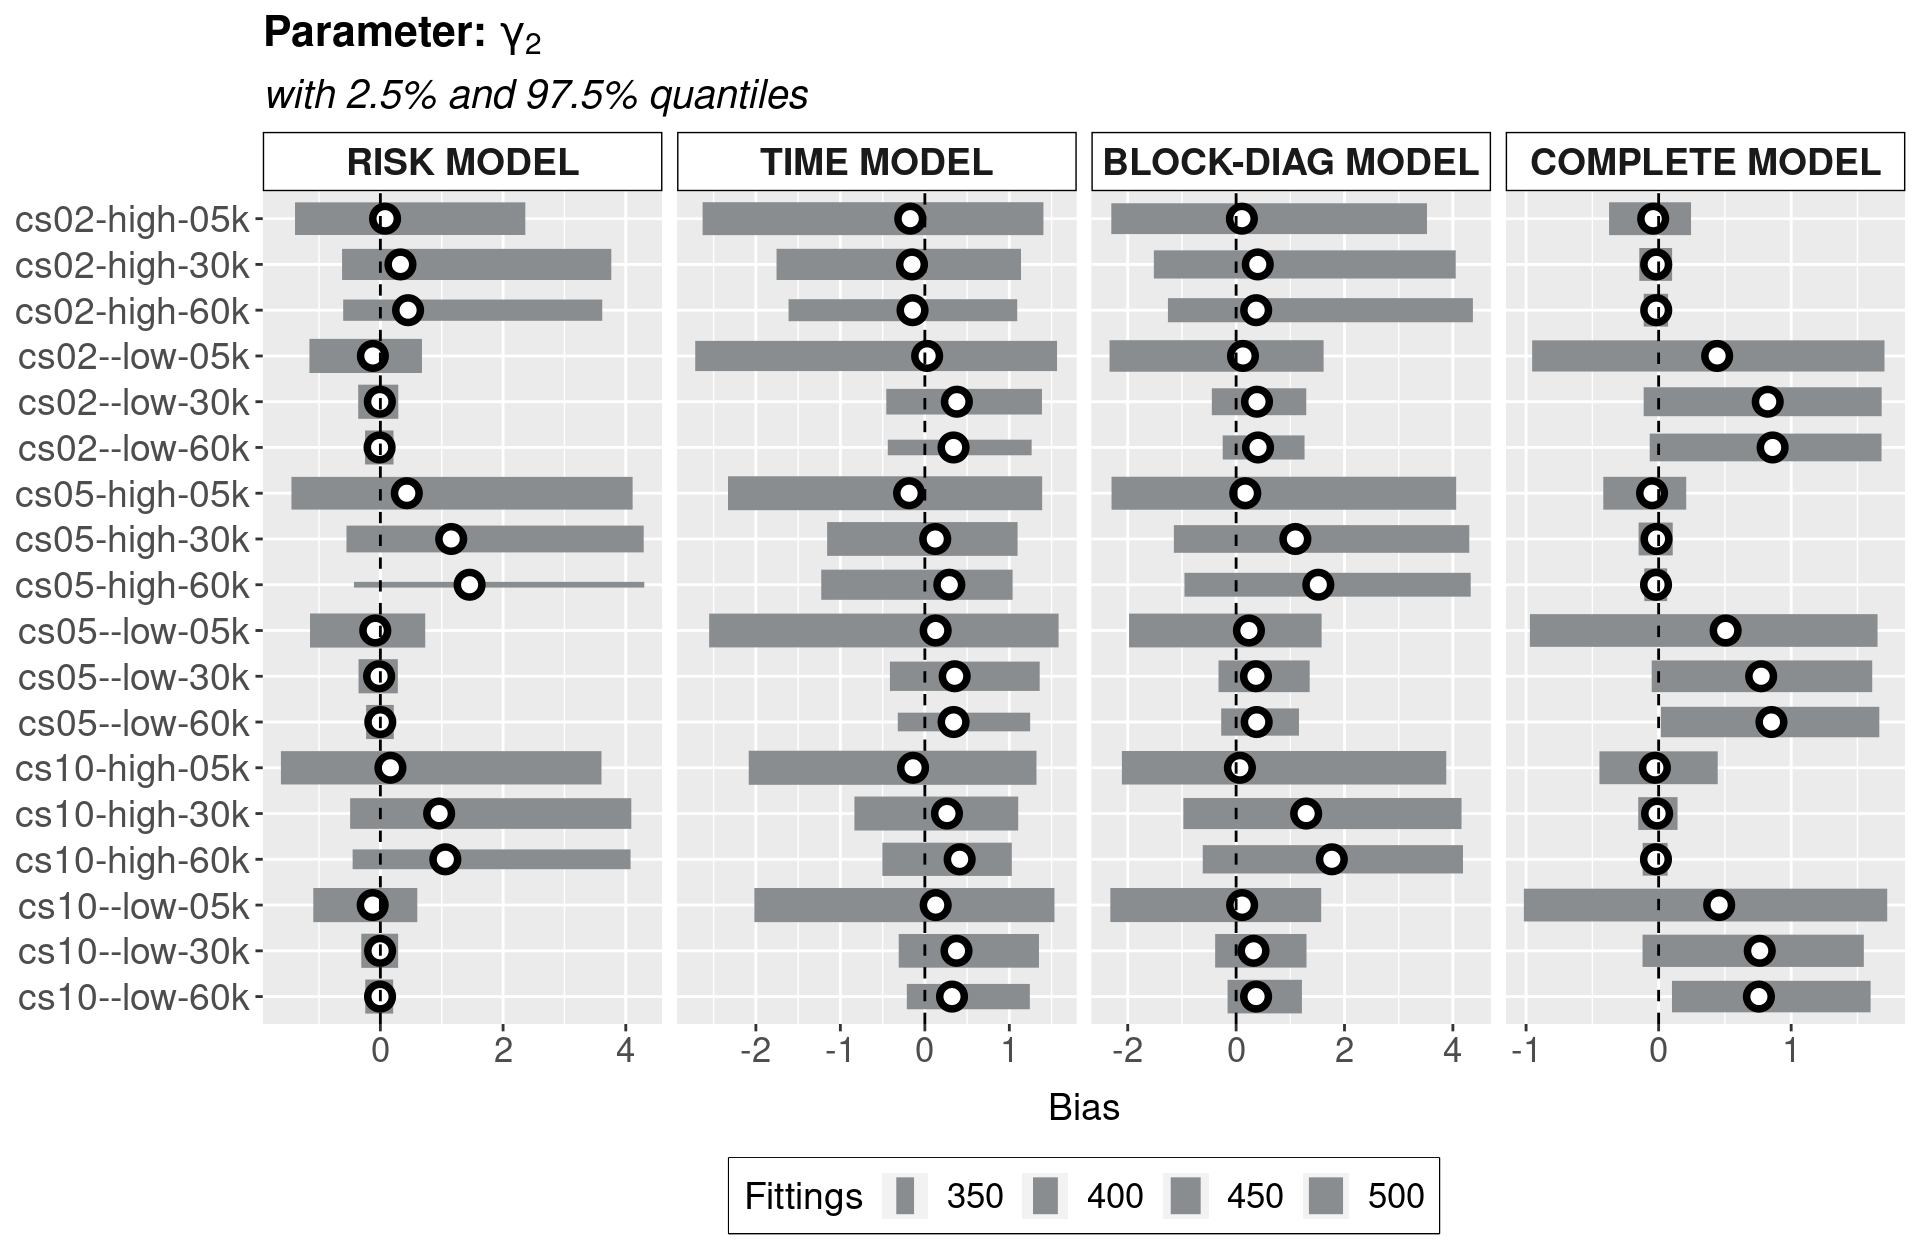
\includegraphics[width=\textwidth]{bias2plot-4.png}\\
 \begin{footnotesize}
  SOURCE: The author (2021).
 \end{footnotesize}
 \label{fig:biasgama2}
\end{figure}

\begin{figure}[H]
 \setlength{\abovecaptionskip}{.0001pt}
 \caption{PARAMETER \(w_{1}\) BIAS WITH 2.5\% AND 97.5\% QUANTILES}
 \vspace{0.2cm}\centering
 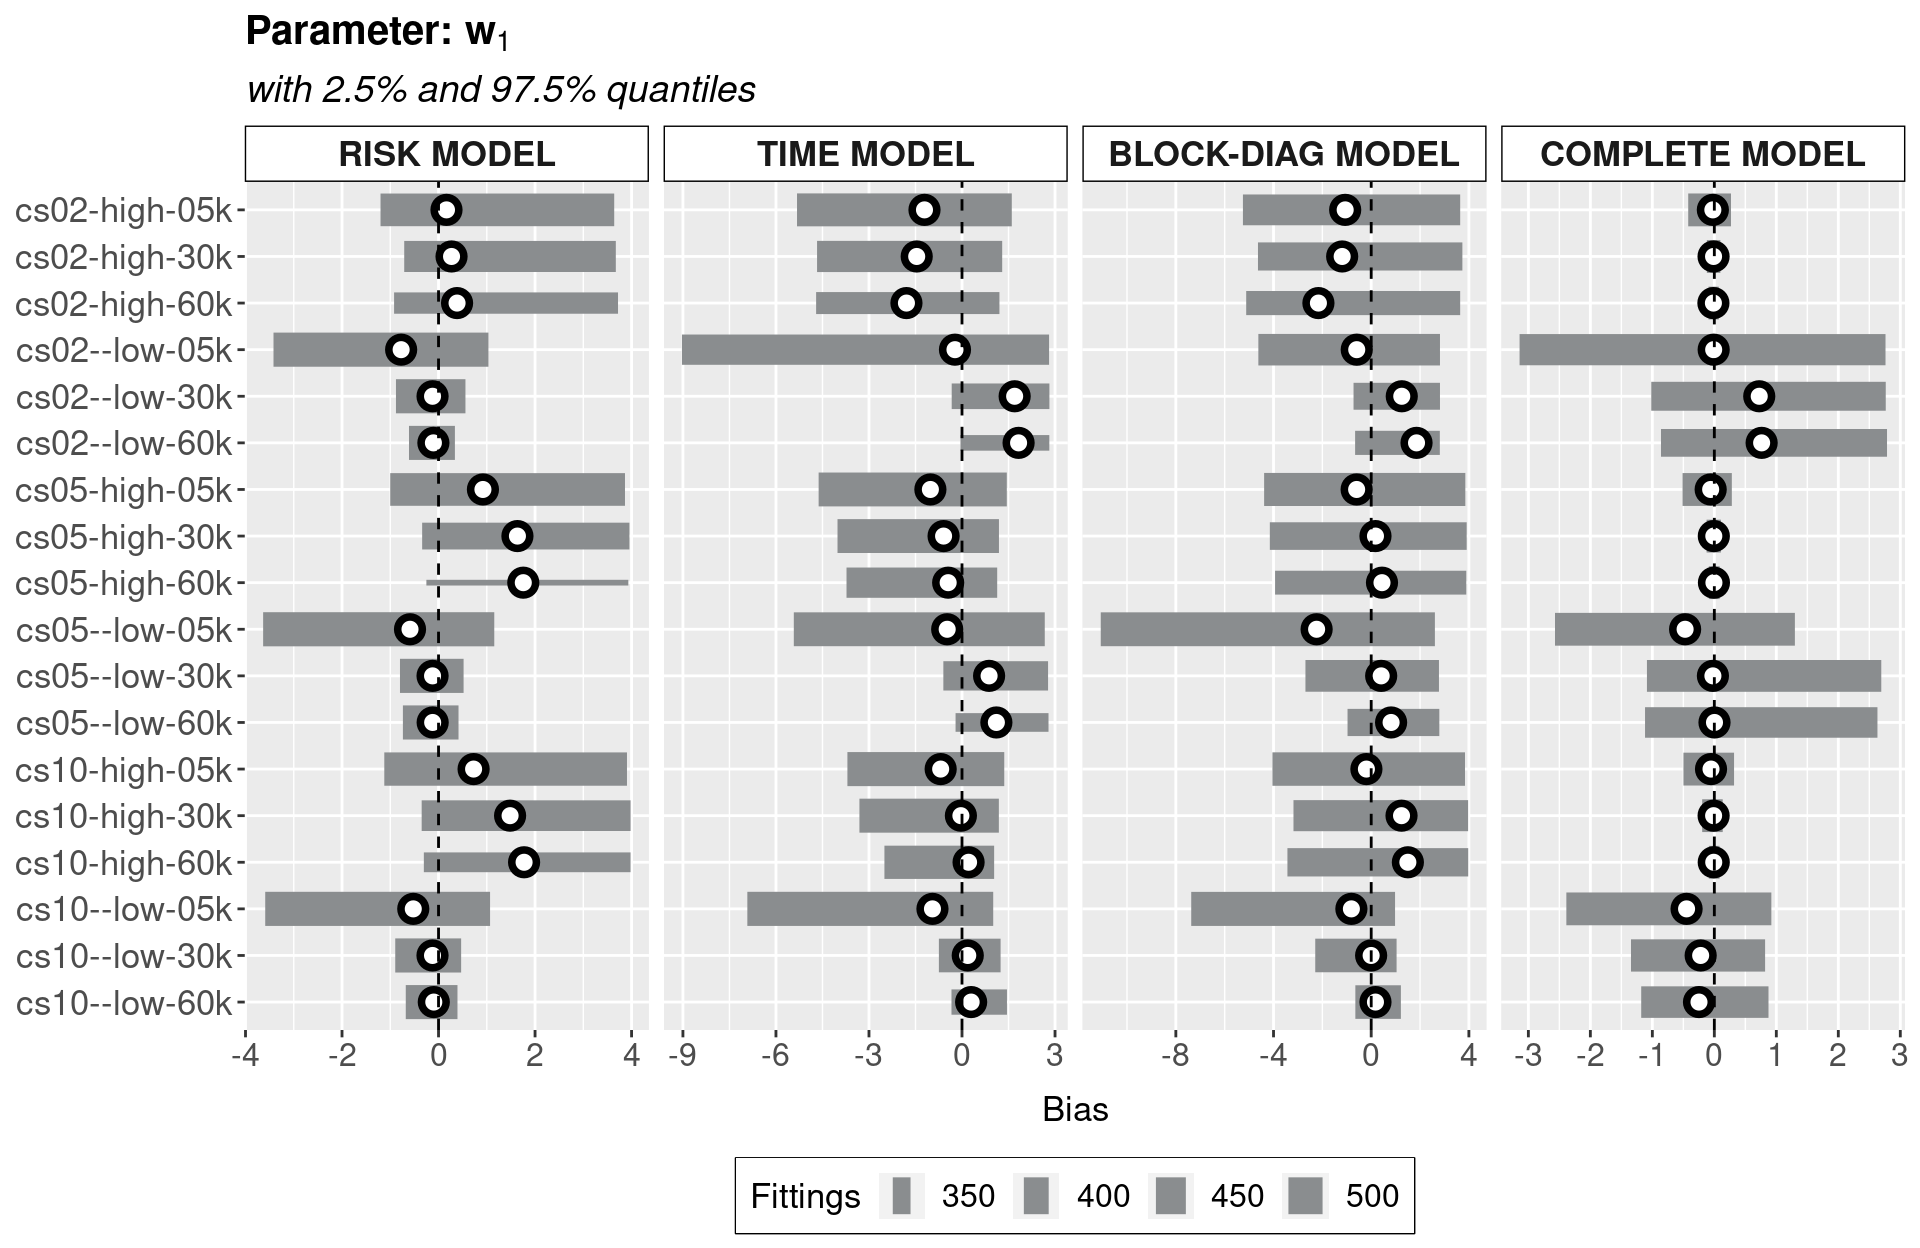
\includegraphics[width=\textwidth]{bias2plot-5.png}\\
 \begin{footnotesize}
  SOURCE: The author (2021).
 \end{footnotesize}
 \label{fig:biasw1}
\end{figure}

\begin{figure}[H]
 \setlength{\abovecaptionskip}{.0001pt}
 \caption{PARAMETER \(w_{2}\) BIAS WITH 2.5\% AND 97.5\% QUANTILES}
 \vspace{0.2cm}\centering
 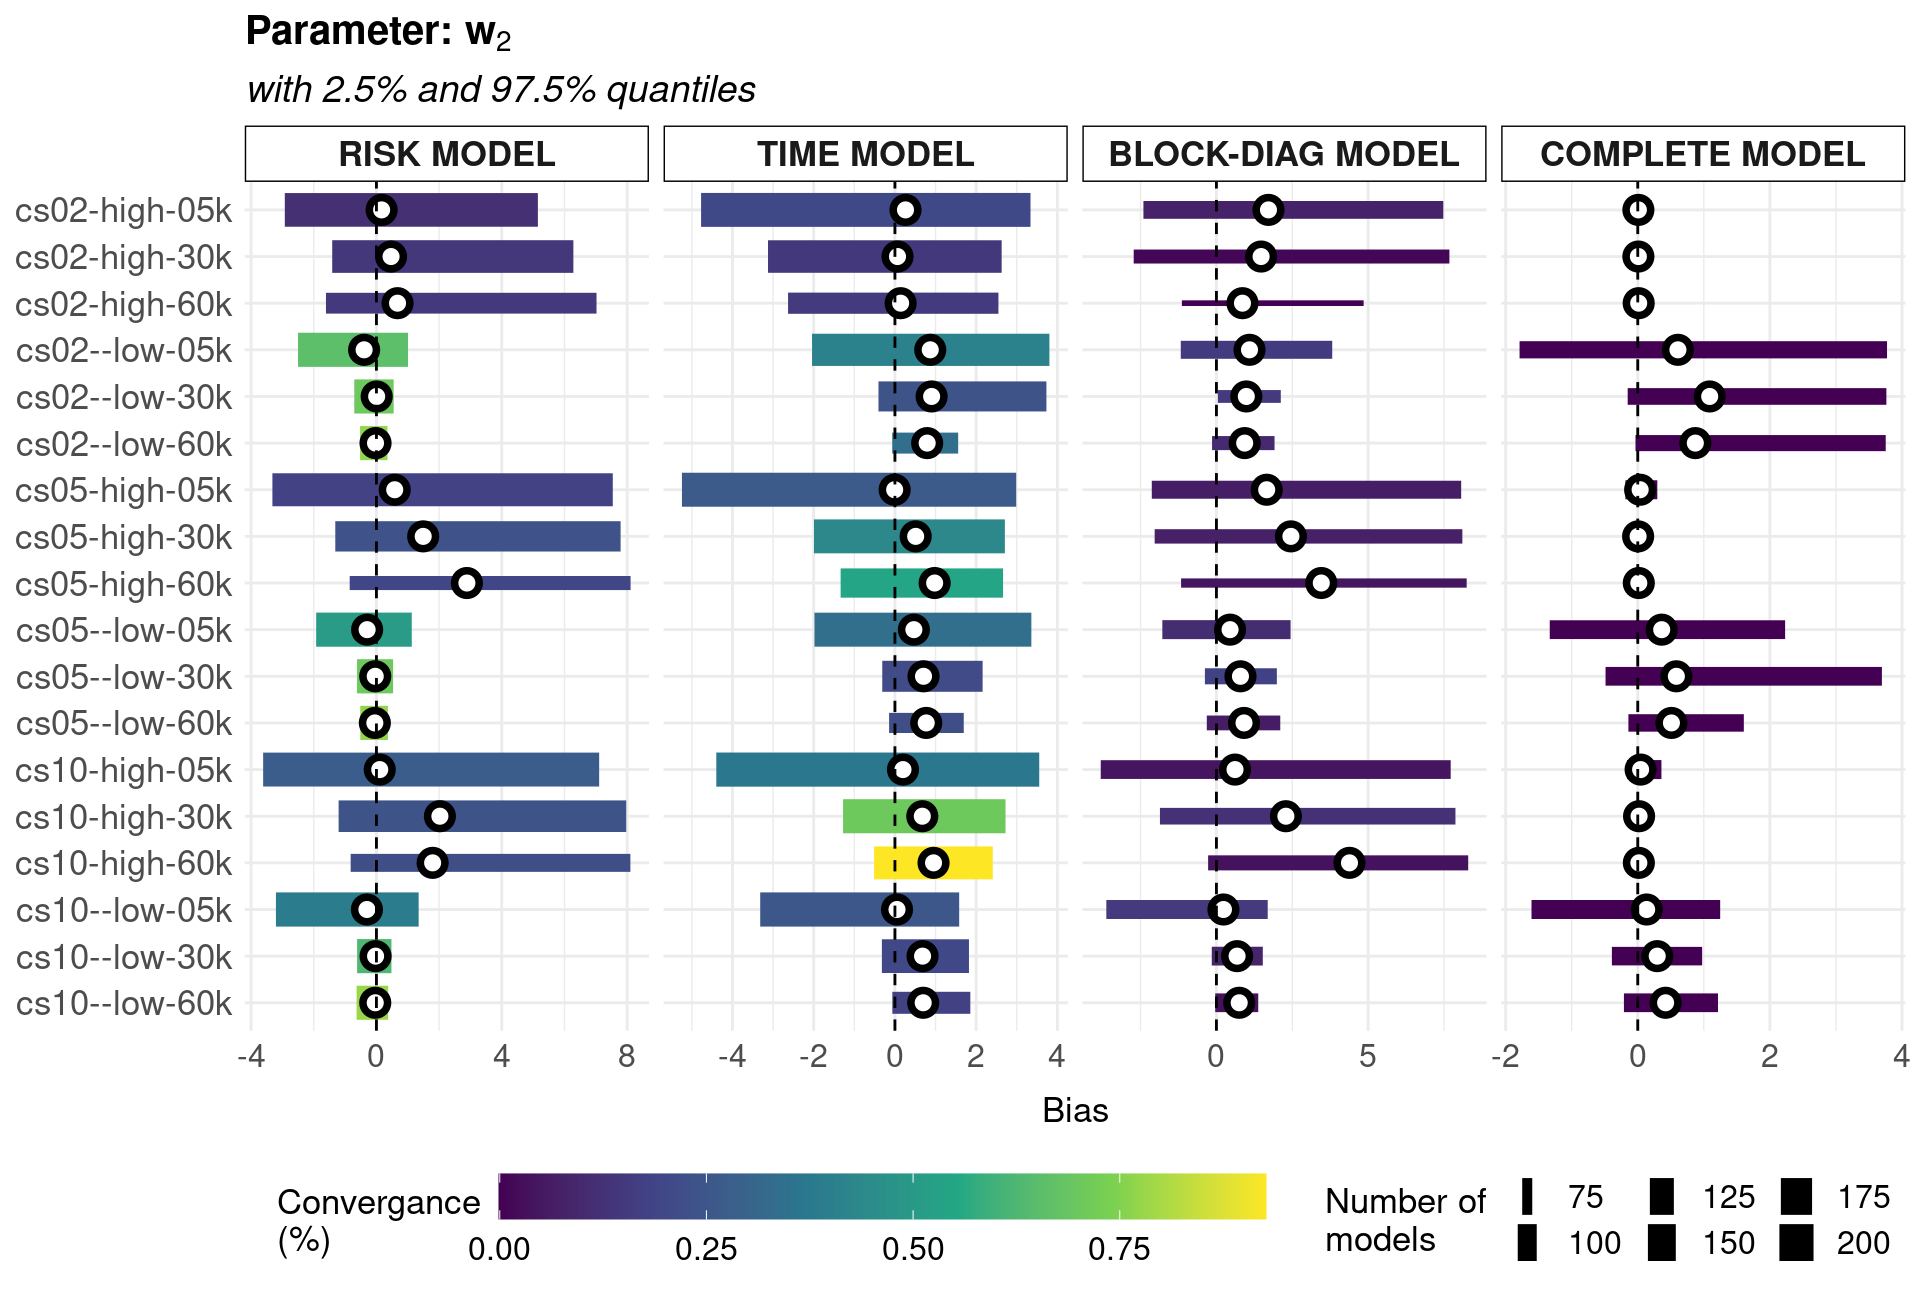
\includegraphics[width=\textwidth]{bias2plot-6.png}\\
 \begin{footnotesize}
  SOURCE: The author (2021).
 \end{footnotesize}
 \label{fig:biasw2}
\end{figure}

\begin{figure}[H]
 \setlength{\abovecaptionskip}{.0001pt}
 \caption{PARAMETER \(\log(\sigma_{1}^{2})\) BIAS WITH 2.5\% AND 97.5\%
          QUANTILES}
 \vspace{0.2cm}\centering
 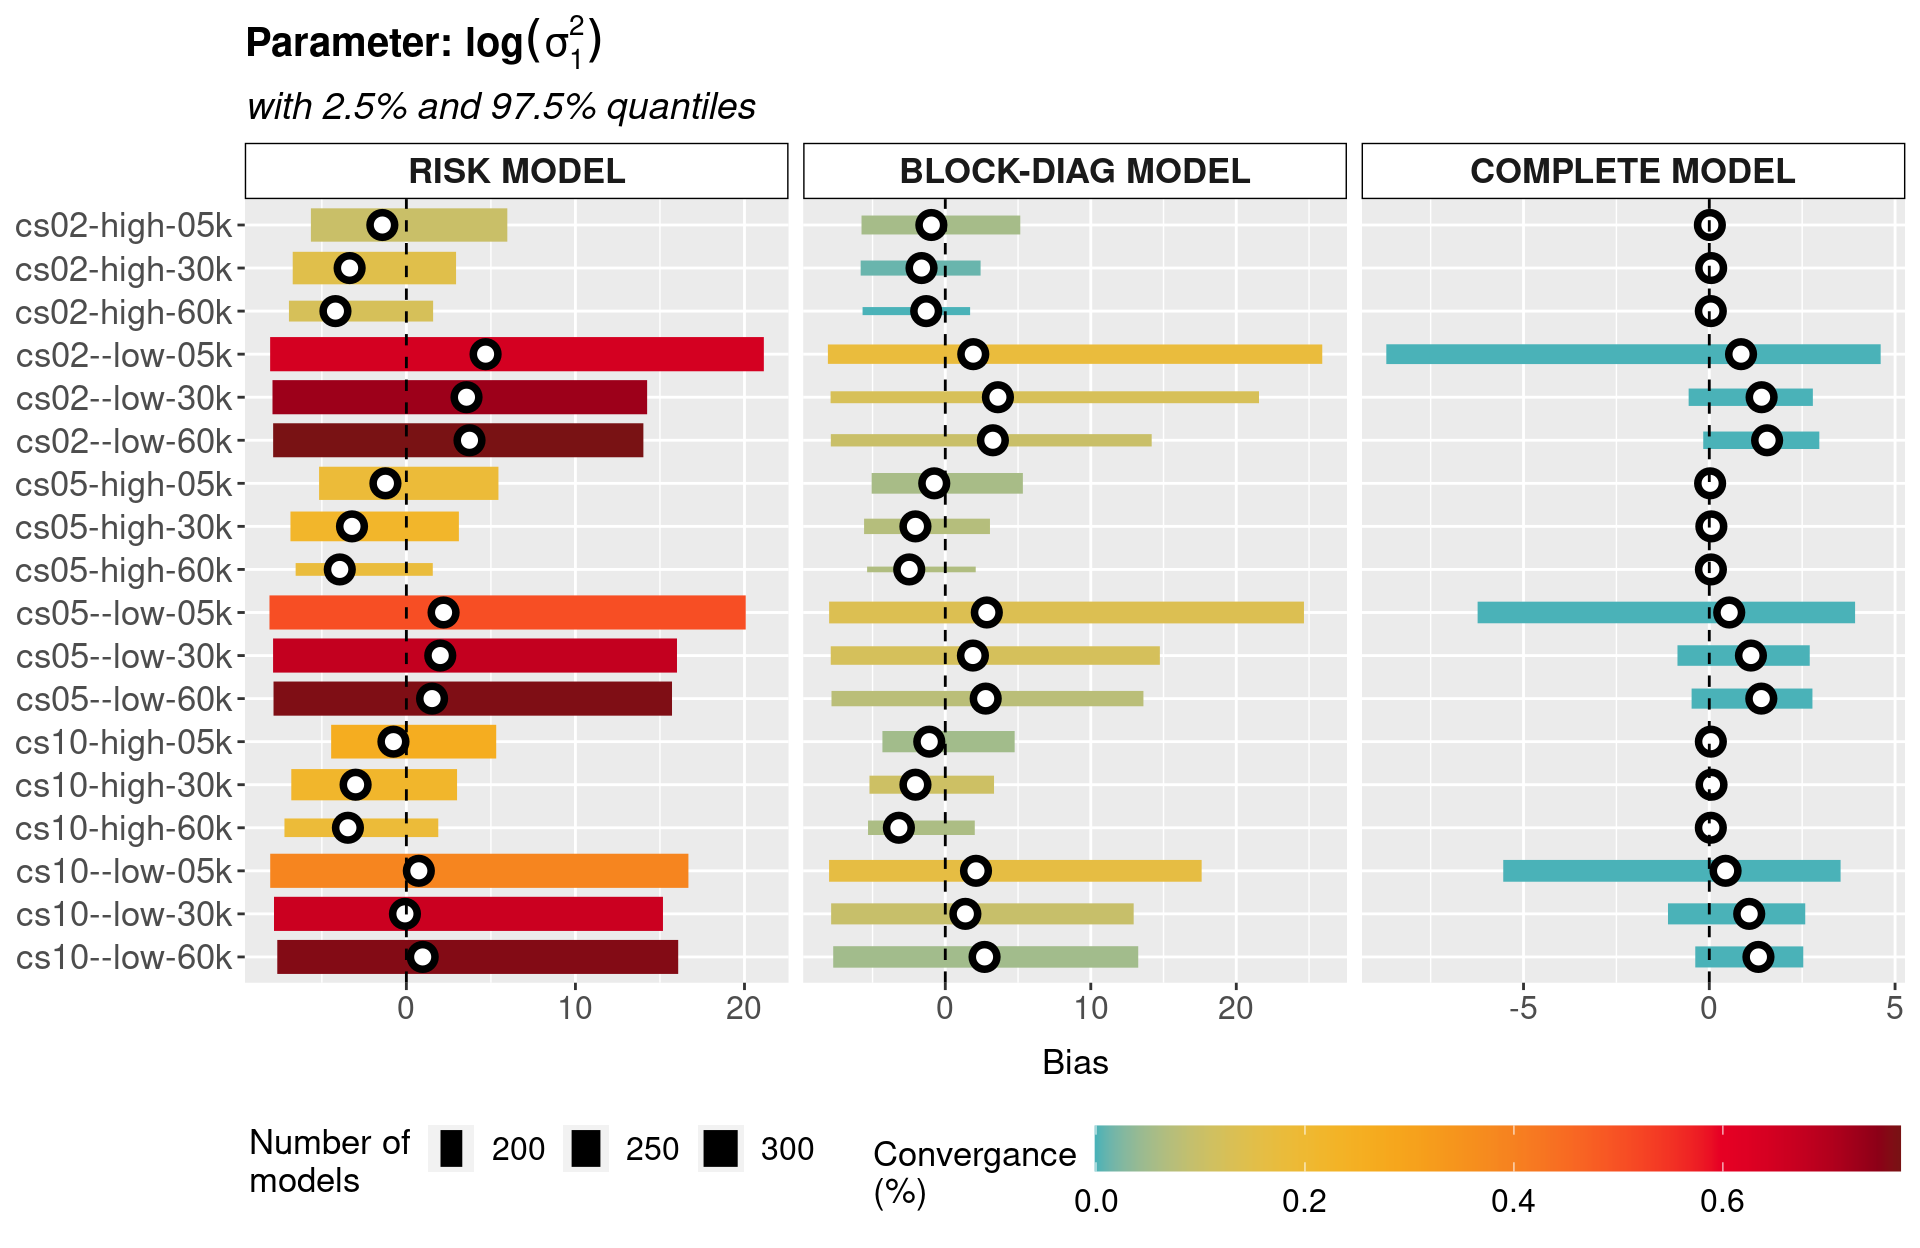
\includegraphics[width=\textwidth]{bias2plot-7.png}\\
 \begin{footnotesize}
  SOURCE: The author (2021).
 \end{footnotesize}
 \label{fig:biaslogs2_1}
\end{figure}

\begin{figure}[H]
 \setlength{\abovecaptionskip}{.0001pt}
 \caption{PARAMETER \(\log(\sigma_{2}^{2})\) BIAS WITH 2.5\% AND 97.5\%
          QUANTILES}
 \vspace{0.2cm}\centering
 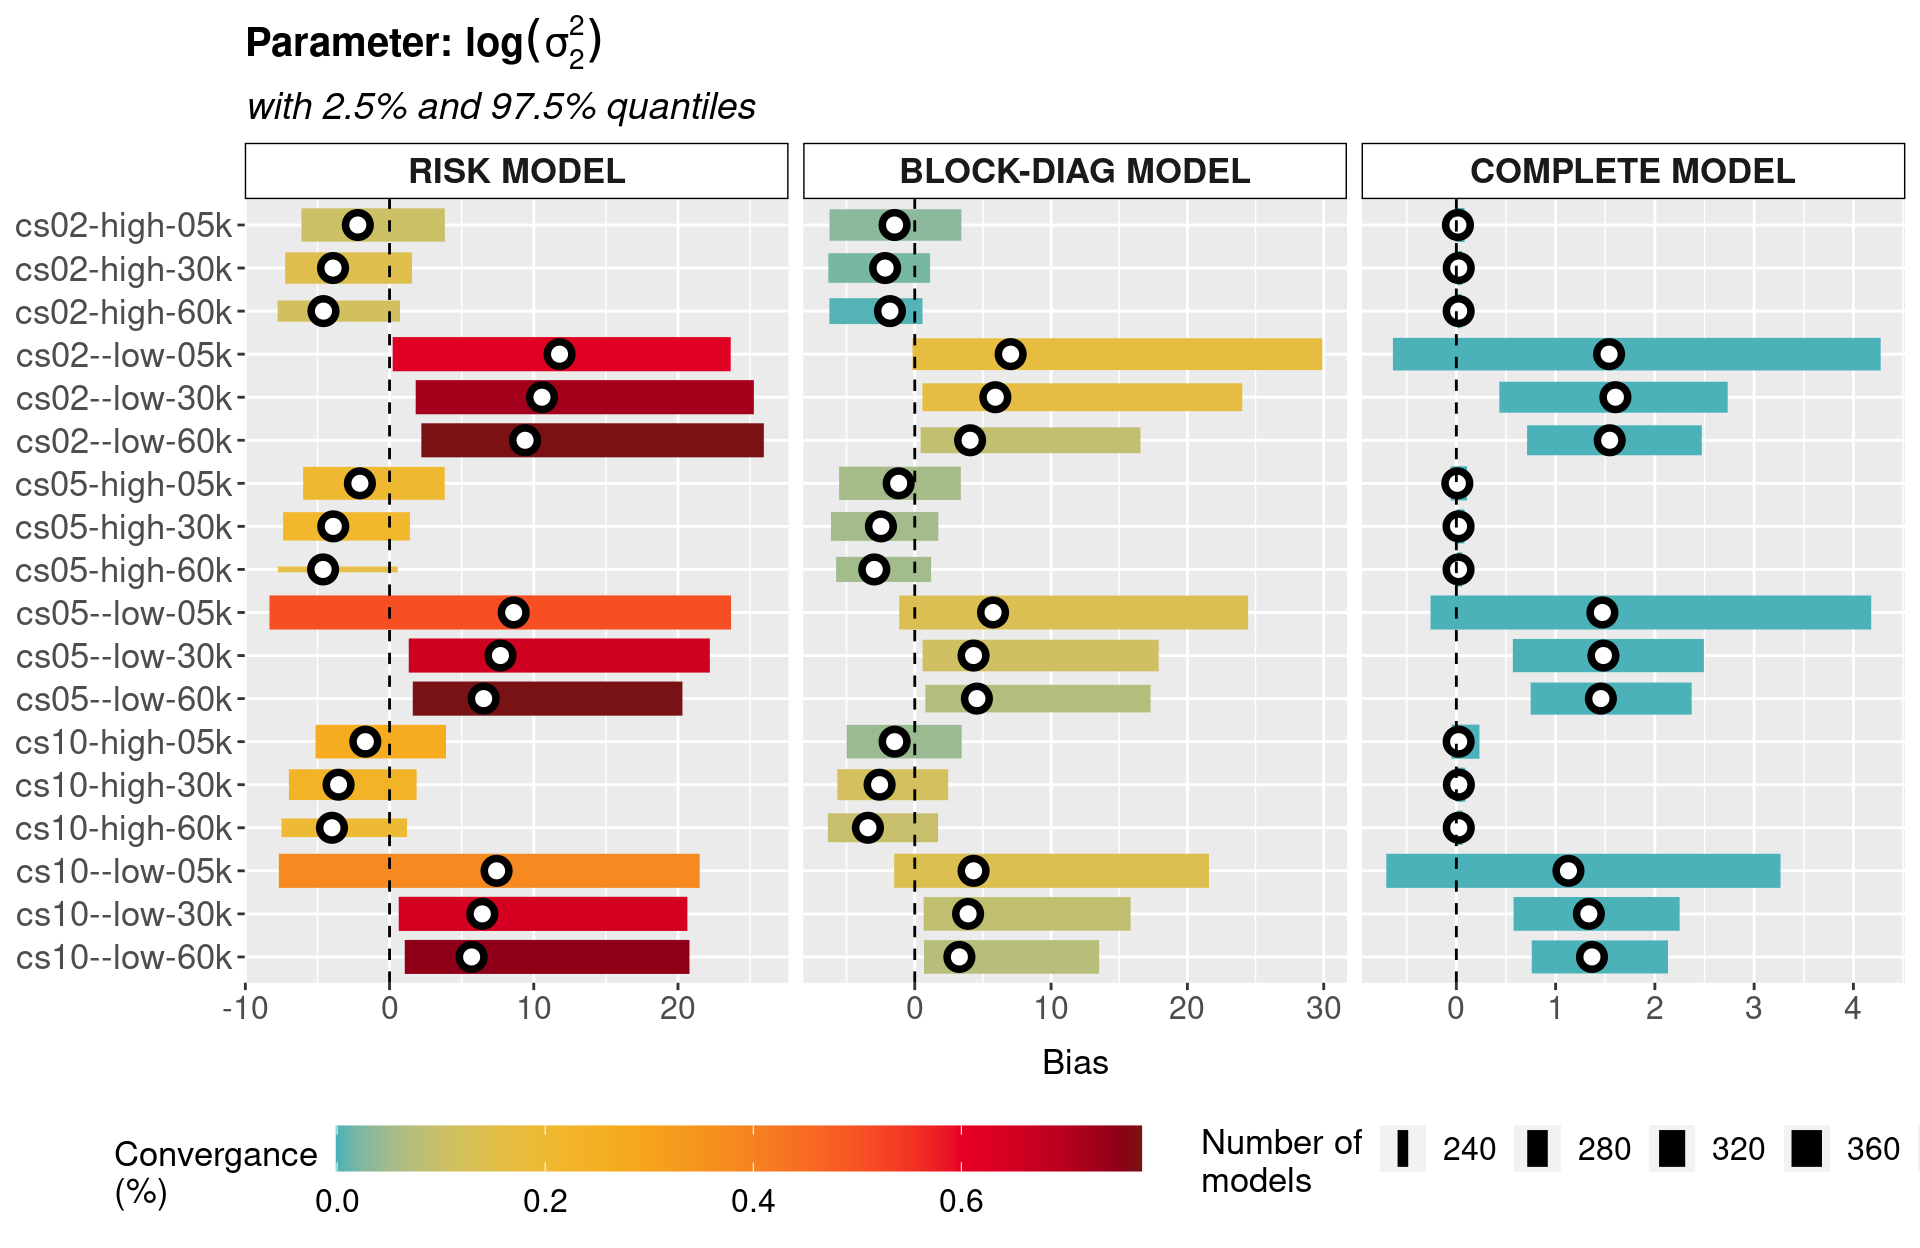
\includegraphics[width=\textwidth]{bias2plot-8.png}\\
 \begin{footnotesize}
  SOURCE: The author (2021).
 \end{footnotesize}
 \label{fig:biaslogs2_2}
\end{figure}

\begin{figure}[H]
 \setlength{\abovecaptionskip}{.0001pt}
 \caption{PARAMETER \(\log(\sigma_{3}^{2})\) BIAS WITH 2.5\% AND 97.5\%
          QUANTILES}
 \vspace{0.2cm}\centering
 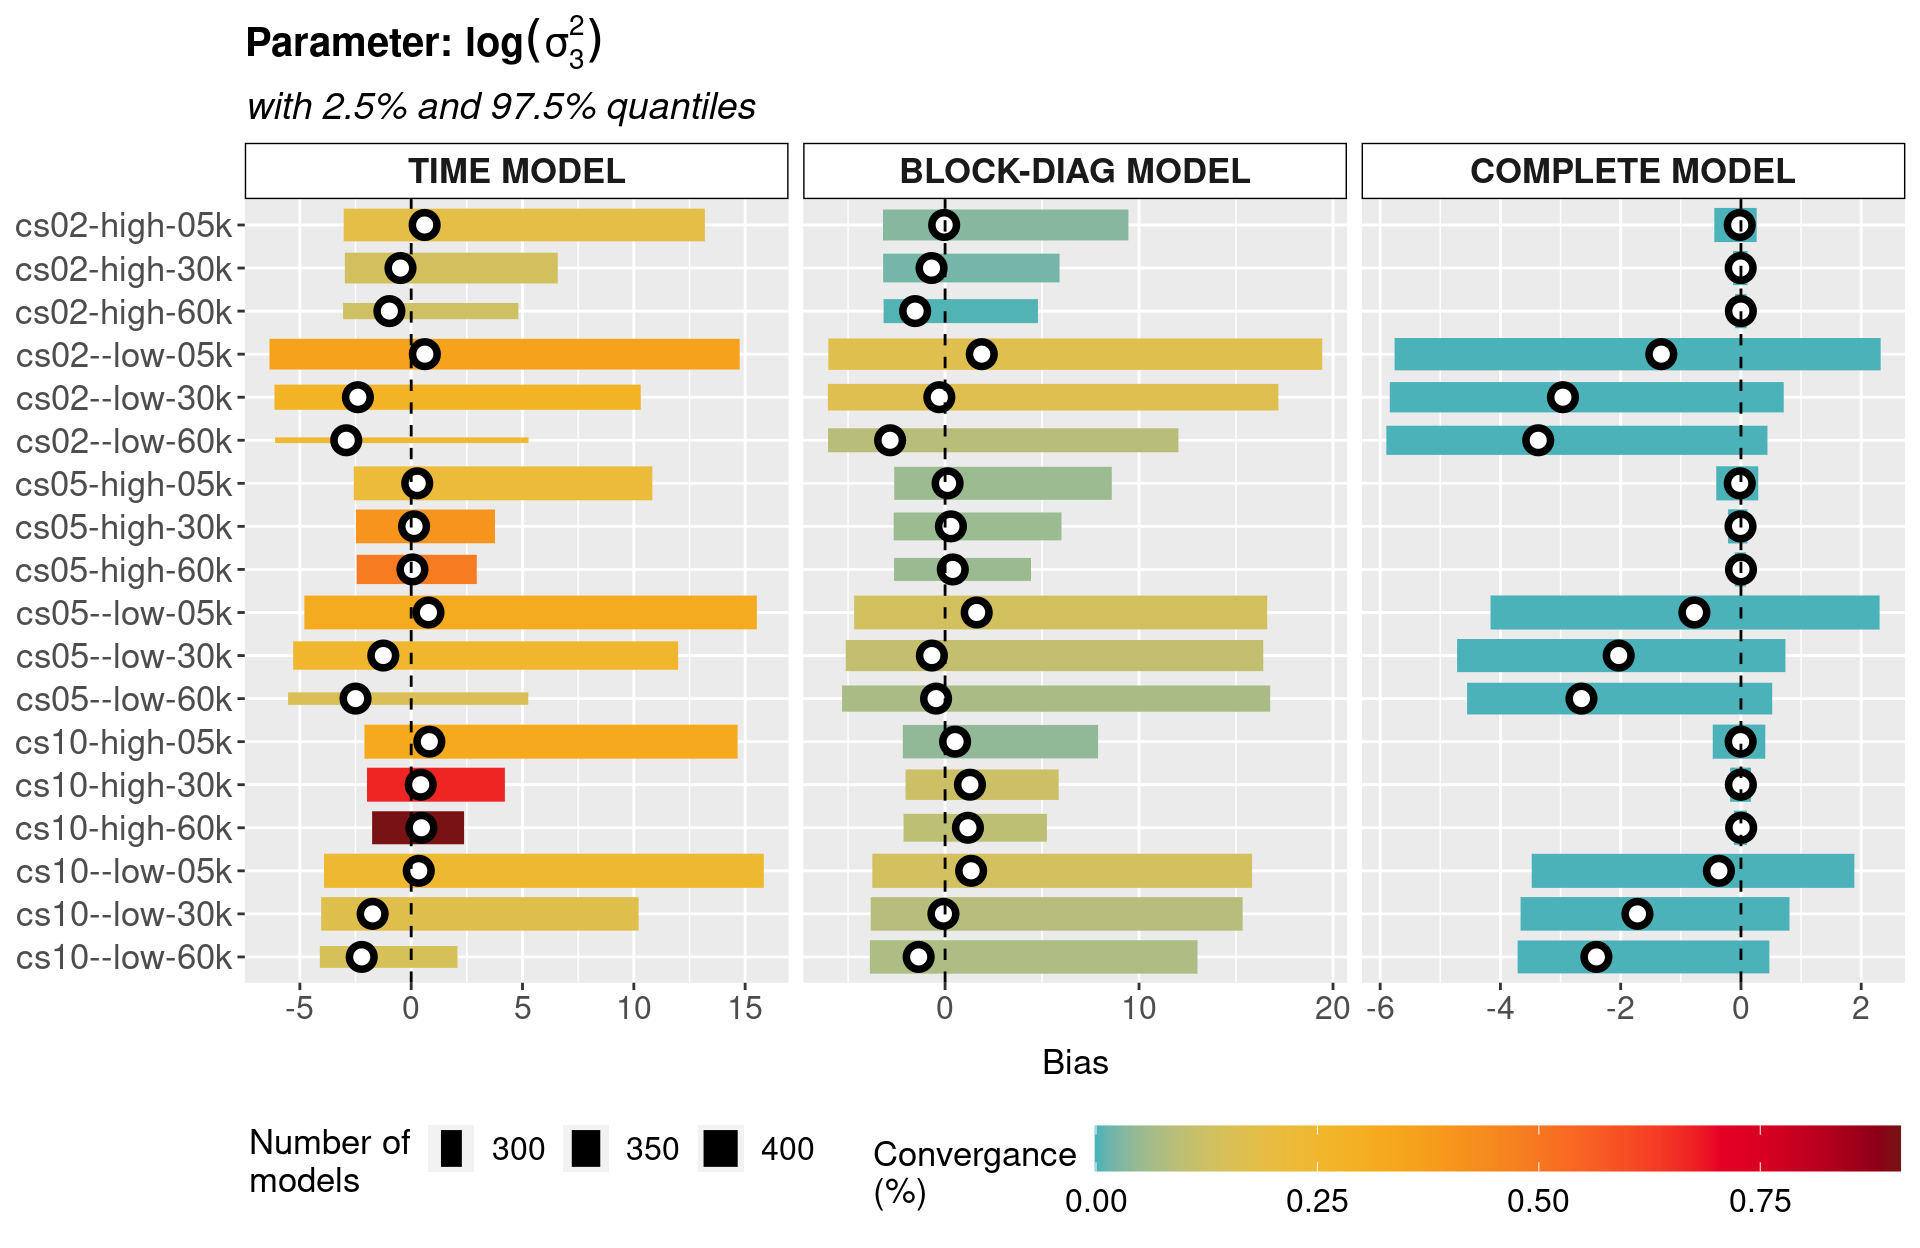
\includegraphics[width=\textwidth]{bias2plot-9.png}\\
 \begin{footnotesize}
  SOURCE: The author (2021).
 \end{footnotesize}
 \label{fig:biaslogs2_3}
\end{figure}

\begin{figure}[H]
 \setlength{\abovecaptionskip}{.0001pt}
 \caption{PARAMETER \(\log(\sigma_{4}^{2})\) BIAS WITH 2.5\% AND 97.5\%
          QUANTILES}
 \vspace{0.2cm}\centering
 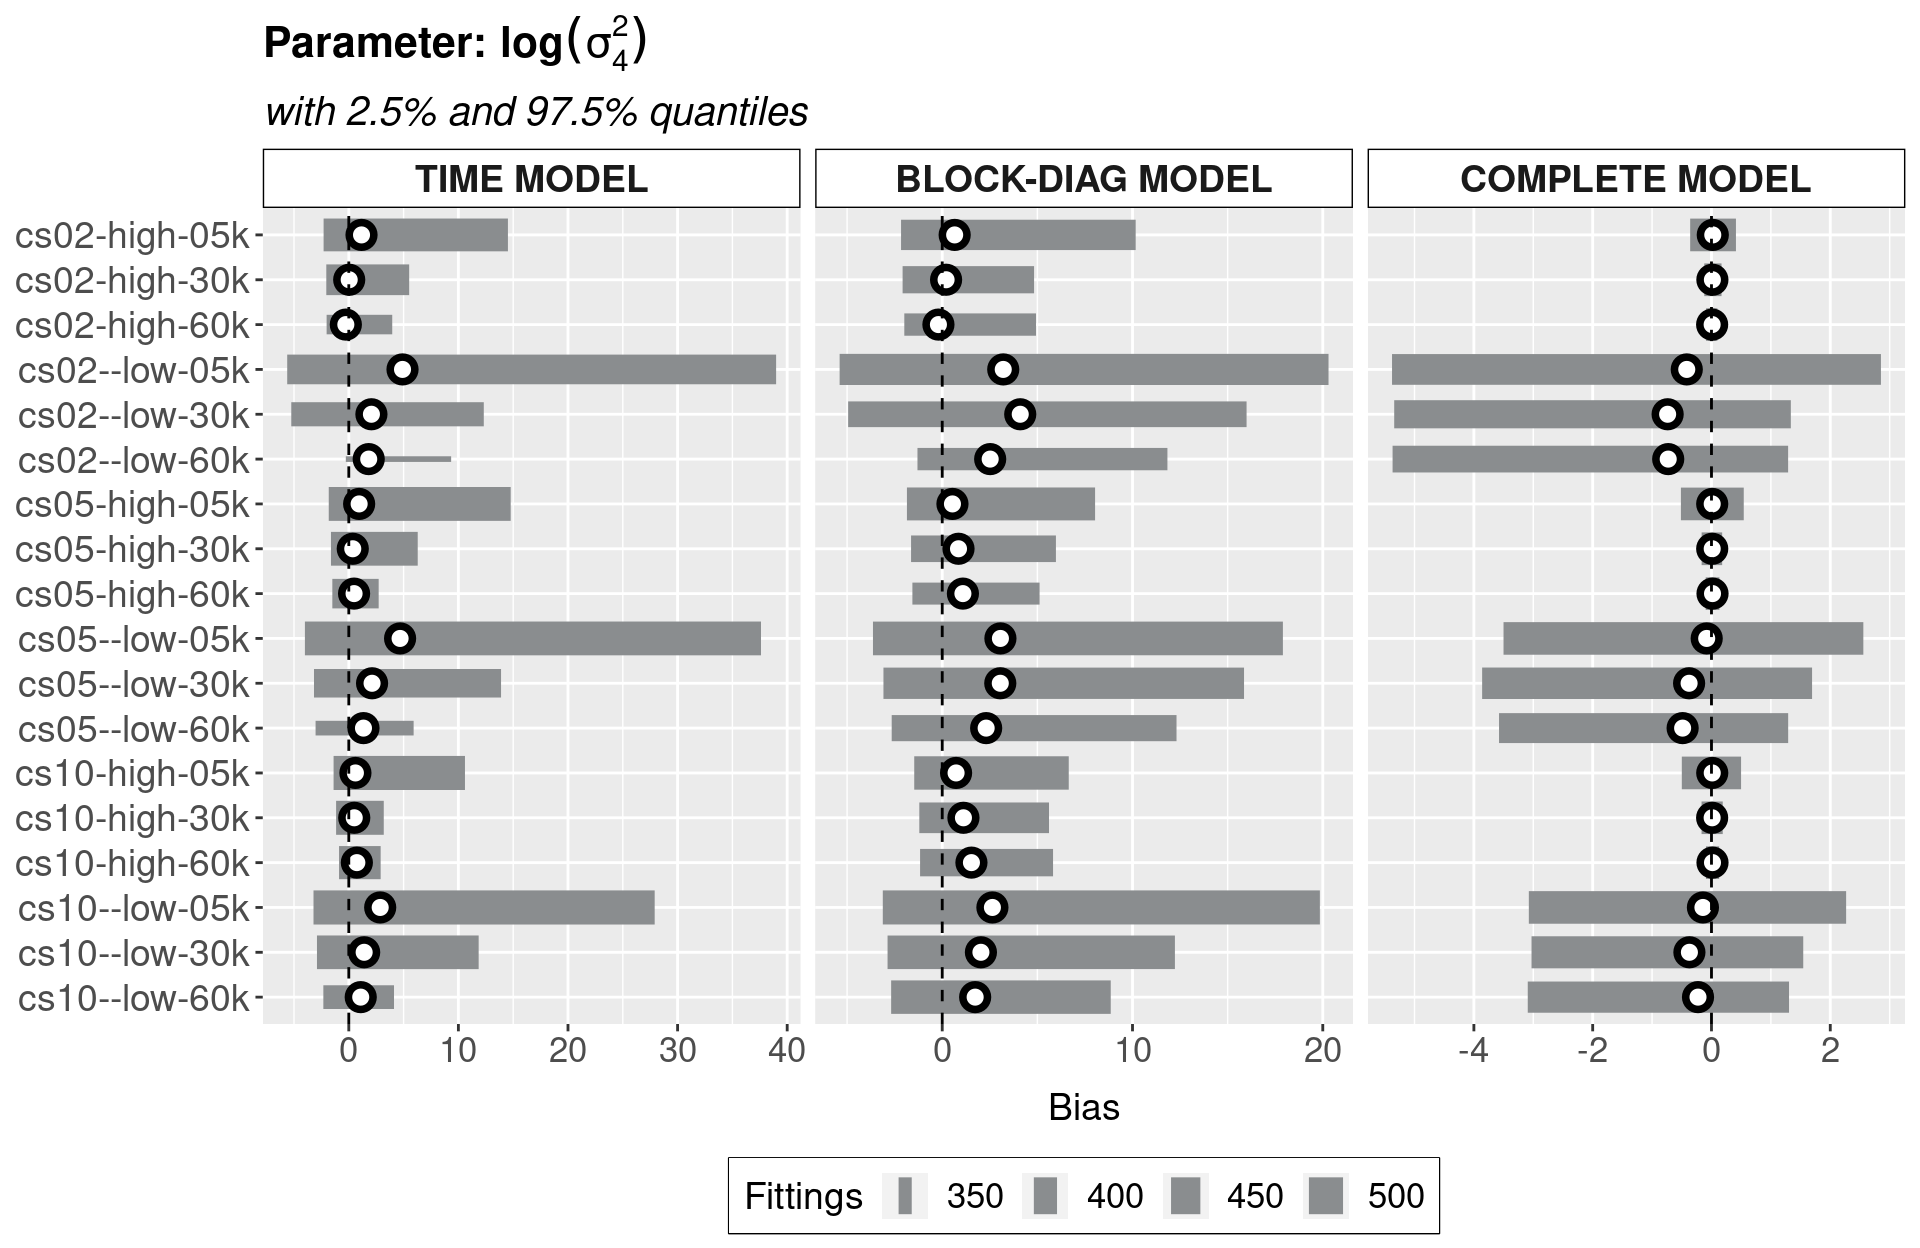
\includegraphics[width=\textwidth]{bias2plot-10.png}\\
 \begin{footnotesize}
  SOURCE: The author (2021).
 \end{footnotesize}
 \label{fig:biaslogs2_4}
\end{figure}

\begin{figure}[H]
 \setlength{\abovecaptionskip}{.0001pt}
 \caption{PARAMETER \(z(\rho_{12})\) BIAS WITH 2.5\% AND 97.5\%
          QUANTILES}
 \vspace{0.2cm}\centering
 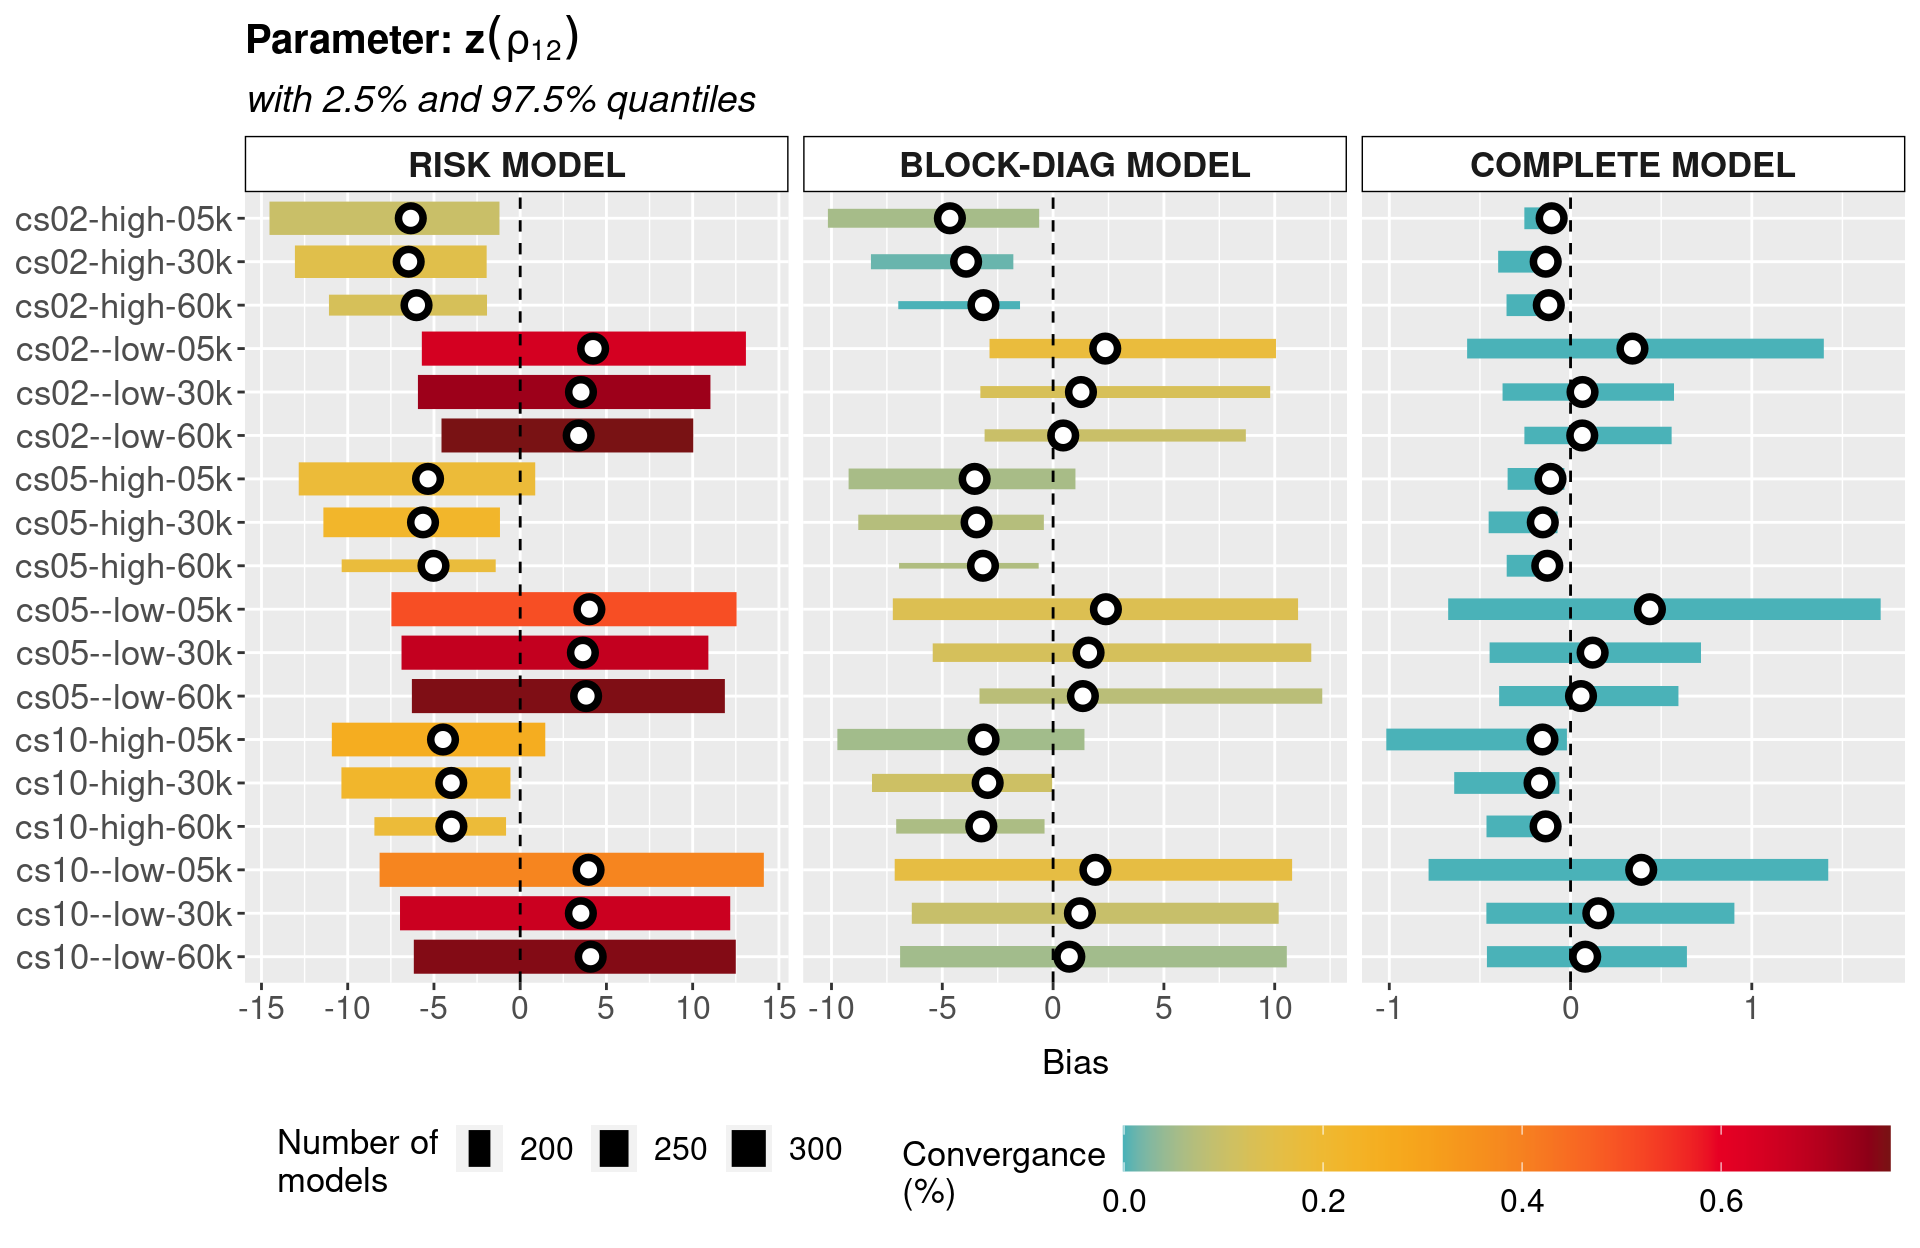
\includegraphics[width=\textwidth]{bias2plot-11.png}\\
 \begin{footnotesize}
  SOURCE: The author (2021).
 \end{footnotesize}
 \label{fig:biasrhoz12}
\end{figure}

\begin{figure}[H]
 \setlength{\abovecaptionskip}{.0001pt}
 \caption{PARAMETER \(z(\rho_{34})\) BIAS WITH 2.5\% AND 97.5\%
          QUANTILES}
 \vspace{0.2cm}\centering
 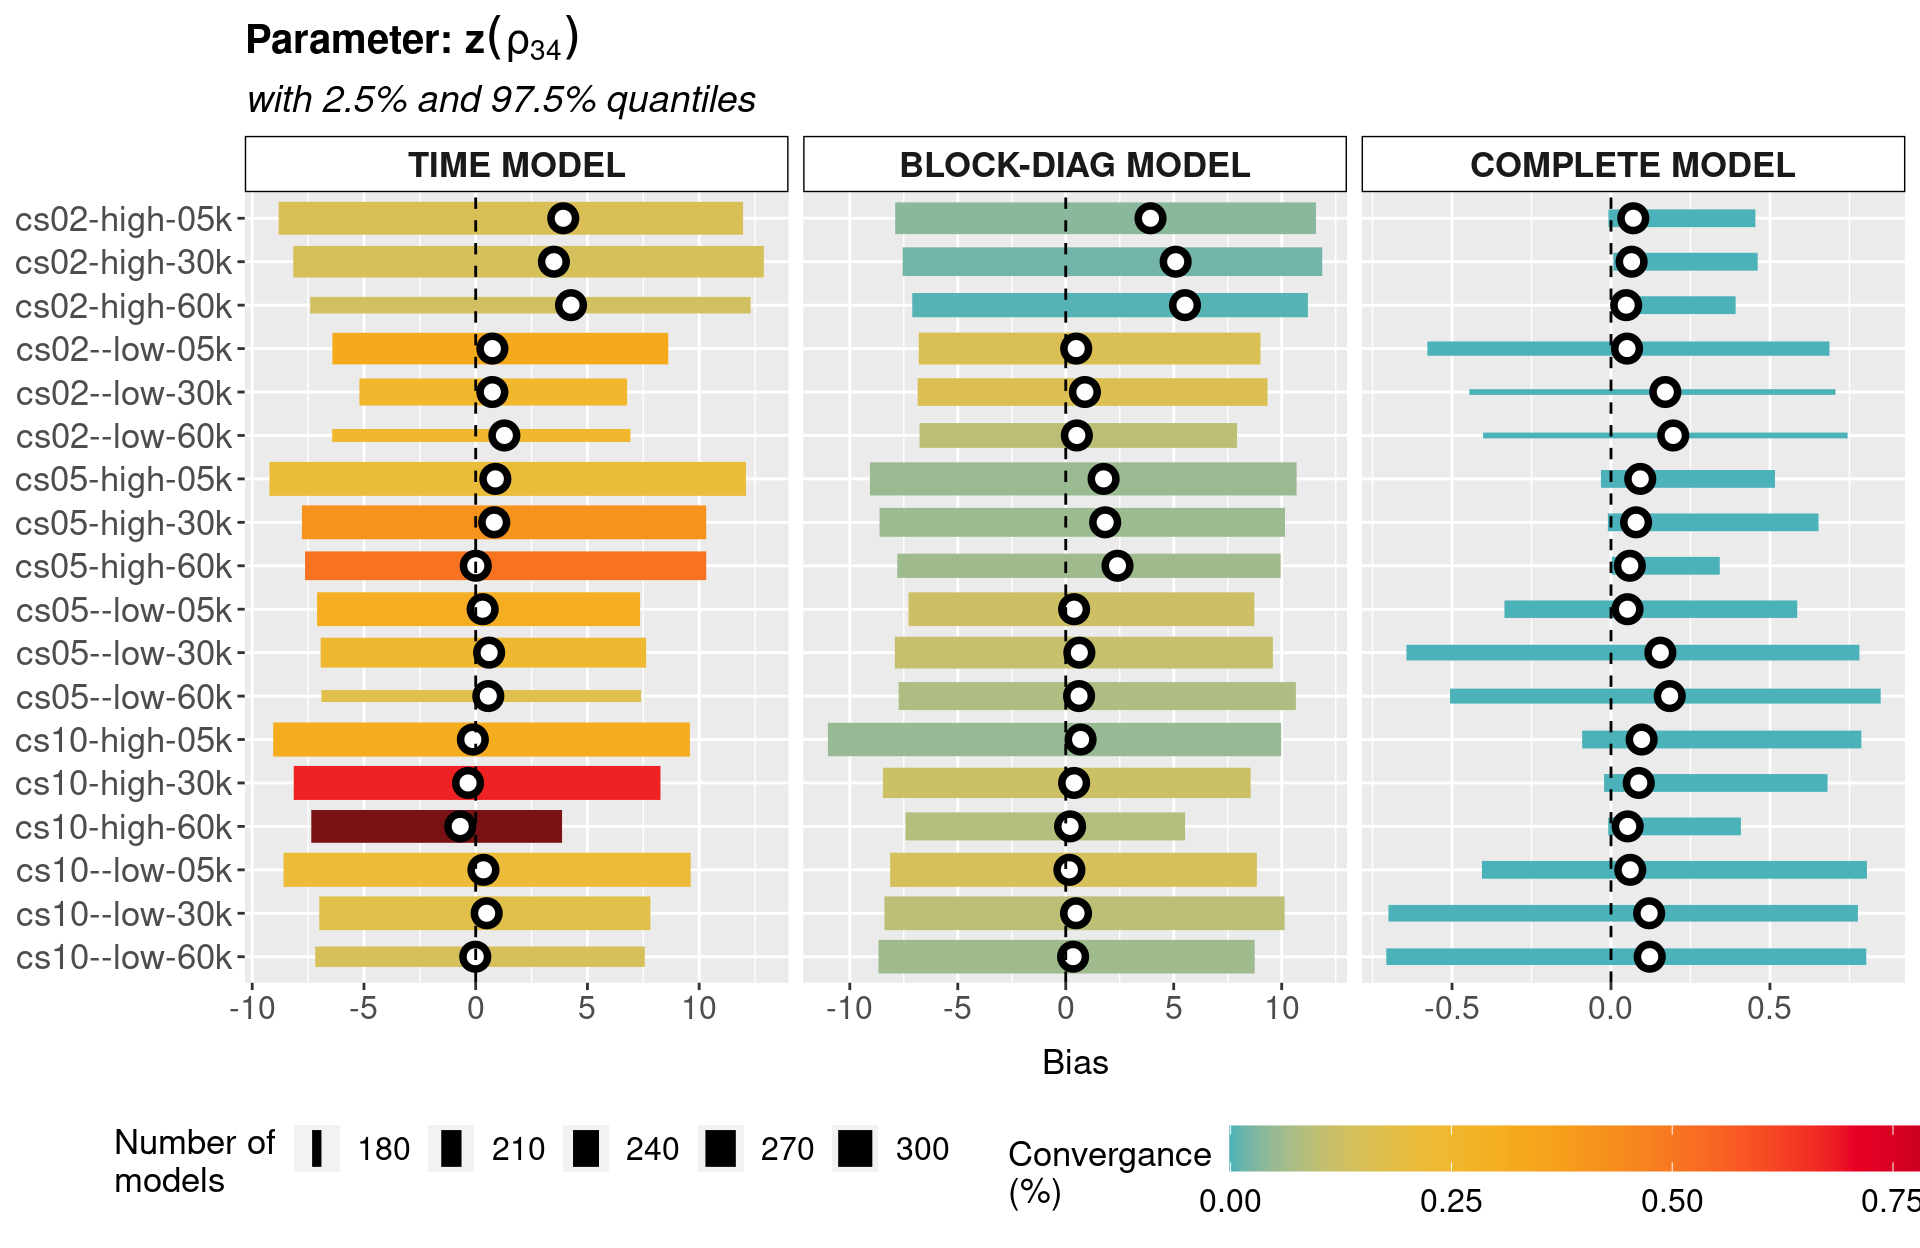
\includegraphics[width=\textwidth]{bias2plot-12.png}\\
 \begin{footnotesize}
  SOURCE: The author (2021).
 \end{footnotesize}
 \label{fig:biasrhoz34}
\end{figure}

\begin{figure}[H]
 \setlength{\abovecaptionskip}{.0001pt}
 \caption{PARAMETERS
          \(\{z(\rho_{13}),~z(\rho_{24}),~z(\rho_{14}),~z(\rho_{23})\}\)
          BIAS WITH 2.5\% AND 97.5\% QUANTILES}
 \vspace{0.2cm}\centering
 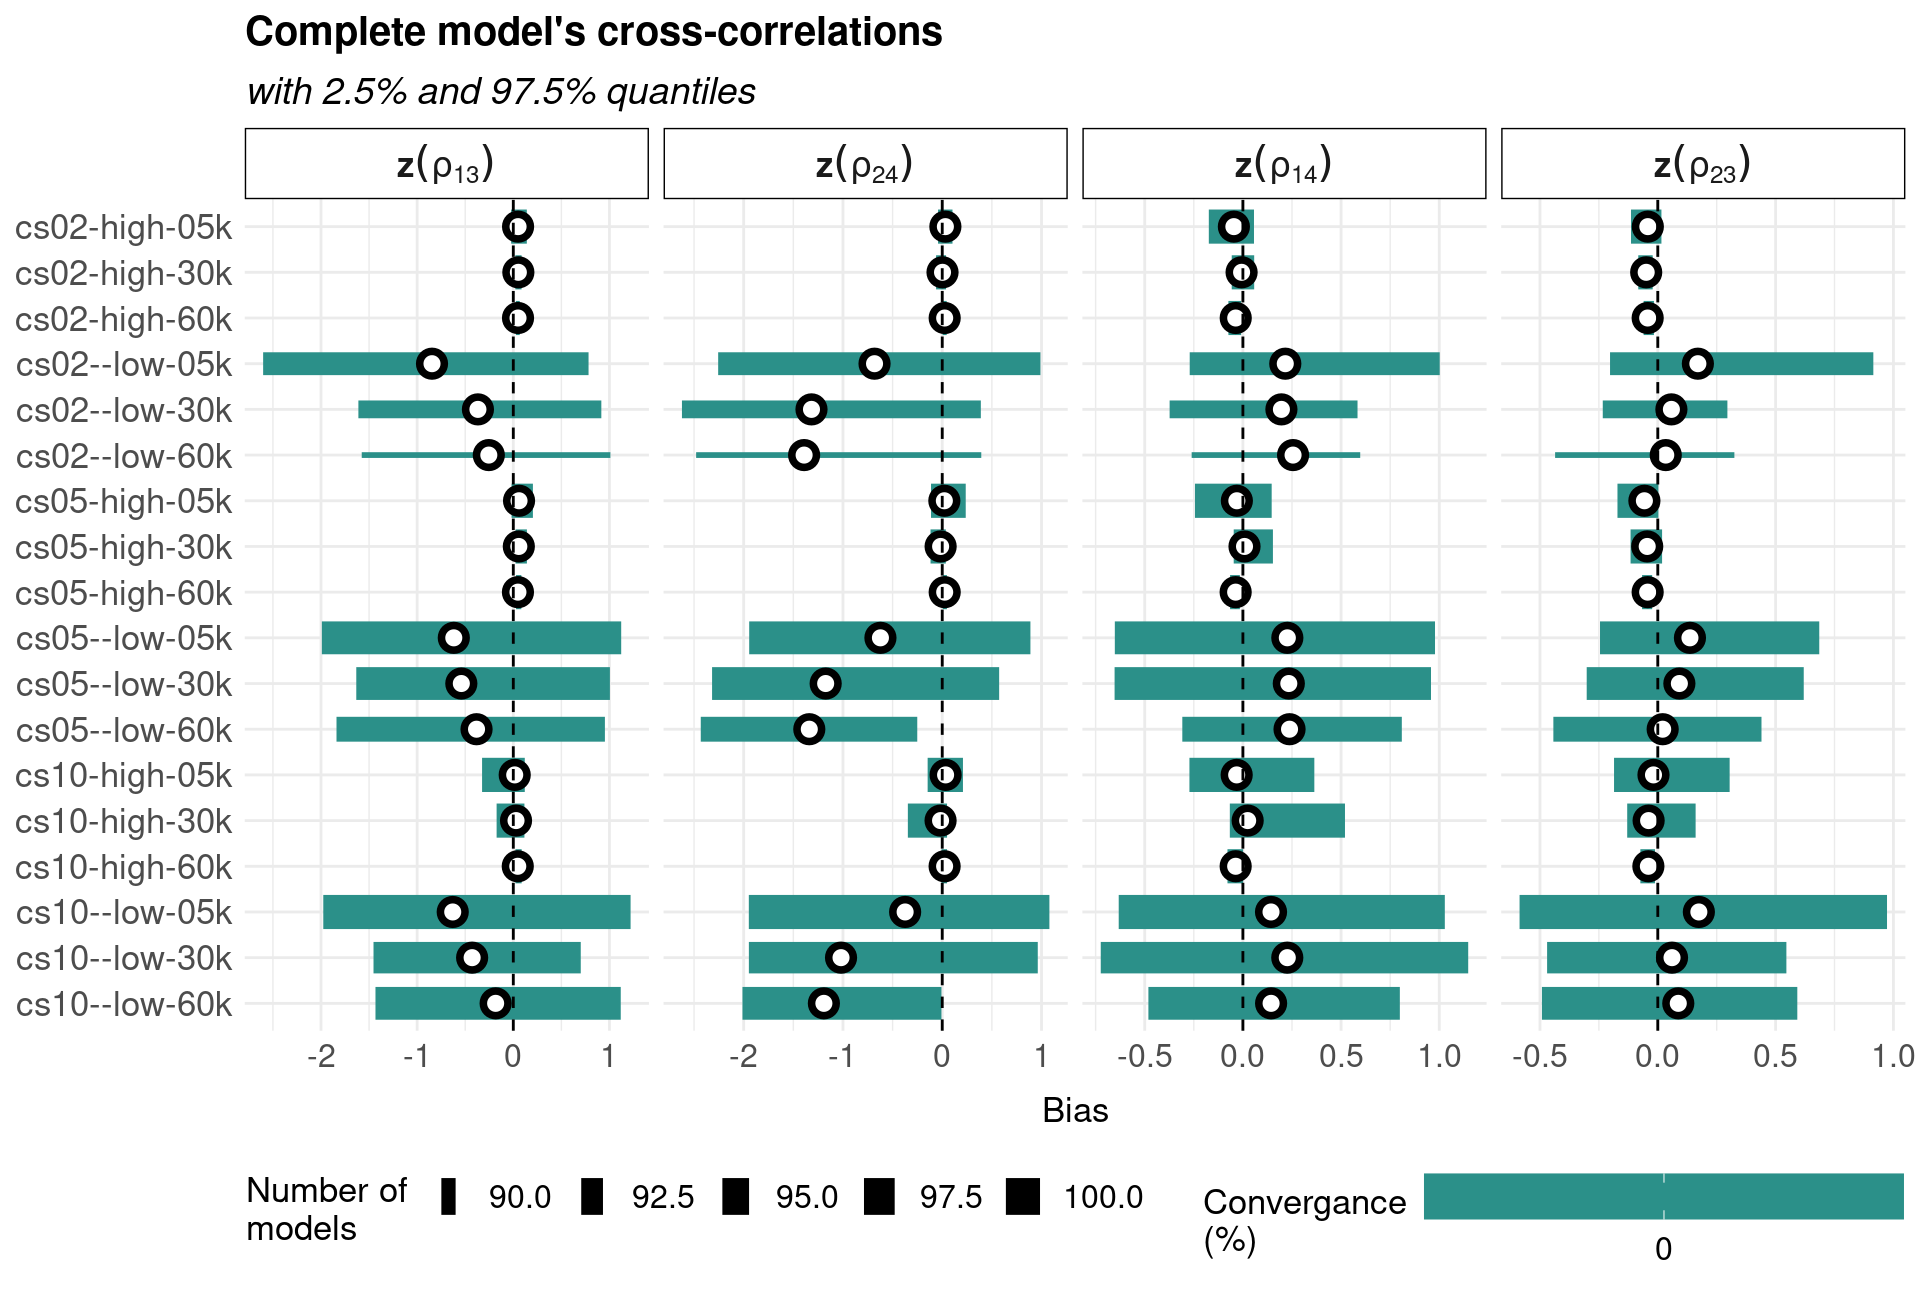
\includegraphics[width=\textwidth]{bias2plot-13.png}\\
 \begin{footnotesize}
  SOURCE: The author (2021).
 \end{footnotesize}
 \label{fig:biasrhoz4}
\end{figure}

\end{apendicesenv}
% ----------------------------------------------------------------------
% \begin{anexosenv}
% \partanexos
% \addcontentsline{toc}{chapter}{\hspace{2.105cm}ANNEX}
% \renewcommand{\ABNTEXchapterfontsize}{\ABNTEXsectionfont}
% \end{anexosenv}
%-----------------------------------------------------------------------
\phantompart
\printindex
%-----------------------------------------------------------------------
\end{document}
% END ==================================================================

% ----------------------------------------------------------------------
% pacote para fazer o checkmark
\usepackage{pifont} % http://ctan.org/pkg/pifont
\newcommand{\cmark}{\ding{51}}%
\newcommand{\xmark}{\ding{55}}%
% ----------------------------------------------------------------------
\usepackage{amsmath}
\usepackage{blkarray}
\usepackage{amsfonts}
\usepackage{amssymb}
\usepackage{pdfpages}
% \usepackage{times}
% \usepackage{helvet}
% \renewcommand{\familydefault}{\sfdefault}
% ----------------------------------------------------------------------
\NewDocumentCommand\cc{+u{\cc}}{\ignorespaces}
% ----------------------------------------------------------------------
% controle do espaçamento entre um parágrafo e outro:
\setlength{\parskip}{0.2cm} % tente também \onelineskip
% ----------------------------------------------------------------------
\titulo{MODELING THE CUMULATIVE INCIDENCE FUNCTION OF CLUSTERED
  COMPETING RISKS DATA: A MULTINOMIAL GLMM APPROACH}
\autor{HENRIQUE APARECIDO LAUREANO}
\data{2021}
\instituicao{FEDERAL UNIVERSITY OF PARANÁ}
\orientador{Prof. PhD Wagner Hugo Bonat}
\coorientador{Prof. PhD Paulo Justiniano Ribeiro Jr}
\tipotrabalho{Dissertação (mestrado)}
\preambulo{\small{Thesis presented to the Graduate Program of Numerical
    Methods in Engineering, Concentration Area in Mathematical
    Programming: Statistical Methods Applied in Engineering, Federal
    University of Paran\'{a}, as part of the requirements to the
    obtention of the Master's Degree in Sciences.}}
% ----------------------------------------------------------------------
% informações do PDF
\makeatletter
\hypersetup{
  % pagebackref=true,
  pdftitle={\@title},
  pdfauthor={\@author},
  pdfsubject={\imprimirpreambulo},
  % pdfkeywords = {}{}{}{},
  colorlinks=true, % false: boxed links; true: colored links
  linkcolor=blue, % color of internal links
  citecolor=blue, % color of links to bibliography
  filecolor=magenta, % color of file links
  urlcolor=blue,
  bookmarksdepth=4
}
\addto\captionsenglish{
  % adjusts names from abnTeX2
  \renewcommand{\folhaderostoname}{Title page}
  \renewcommand{\epigraphname}{Epigraph}
  \renewcommand{\dedicatorianame}{Dedication}
  \renewcommand{\errataname}{Errata sheet}
  \renewcommand{\agradecimentosname}{Acknowledgements}
  \renewcommand{\anexoname}{ANNEX}
  \renewcommand{\anexosname}{Annex}
  \renewcommand{\apendicename}{APPENDIX}
  \renewcommand{\apendicesname}{Appendix}
  \renewcommand{\orientadorname}{Supervisor:}
  \renewcommand{\coorientadorname}{Co-supervisor:}
  \renewcommand{\folhadeaprovacaoname}{Approval}
  \renewcommand{\resumoname}{Abstract}
  \renewcommand{\listadesiglasname}{List of abbreviations and acronyms}
  \renewcommand{\listadesimbolosname}{List of symbols}
  \renewcommand{\fontename}{Source}
  \renewcommand{\notaname}{Note}
  % adjusts names used by \autoref
  \renewcommand{\pageautorefname}{page}
  \renewcommand{\chapterautorefname}{Chapter}
  \renewcommand{\sectionautorefname}{Section}
  \renewcommand{\subsectionautorefname}{subsection}
  \renewcommand{\subsubsectionautorefname}{subsubsection}
  \renewcommand{\paragraphautorefname}{subsubsubsection}
}
\makeatother
% ----------------------------------------------------------------------
\graphicspath{{figures/}}
% ----------------------------------------------------------------------
\begin{document}
\selectlanguage{english}
% adequando o uppercase titulo dos elementos nas suas respectivas
% legendas
\renewcommand{\tablename}{TABLE }
\renewcommand{\figurename}{FIGURE }
% ----------------------------------------------------------------------
\frenchspacing % retira espaço extra obsoleto entre as frases
% ----------------------------------------------------------------------
% capa
\tikz[remember picture,overlay] \node[opacity=1,inner sep=0pt] at
(current page.center){
  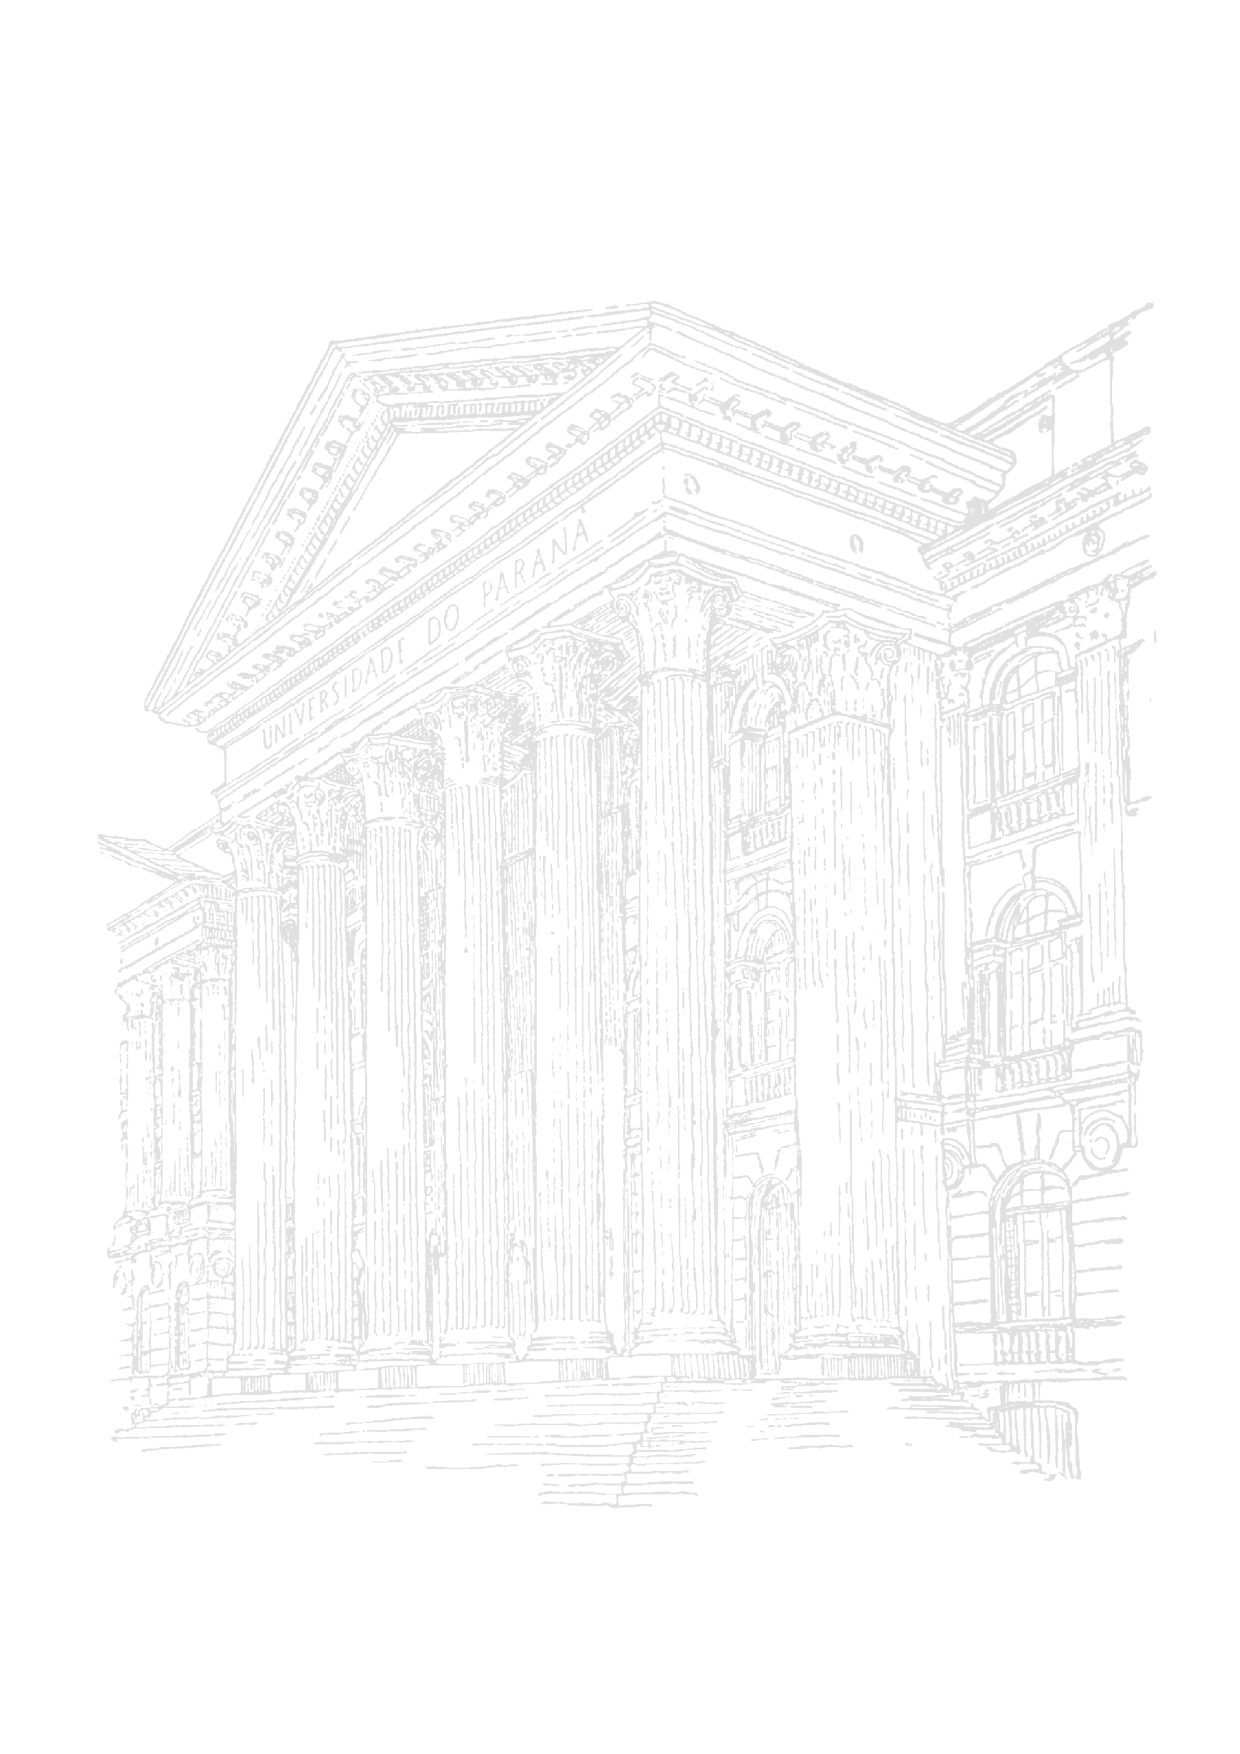
\includegraphics[width=\paperwidth,
  height=\paperheight]{Figuras/ufpr_bg}};
% ----------------------------------------------------------------------
\imprimircapa
% ----------------------------------------------------------------------
% folha de rosto
\imprimirfolhaderosto
% ----------------------------------------------------------------------
% \begin{dedicatoria}
%   \vspace*{\fill}
%   ...
%   \vspace*{\fill}
% \end{dedicatoria}
% ----------------------------------------------------------------------
% ficha catalográfica

% \begin{fichacatalografica}
%   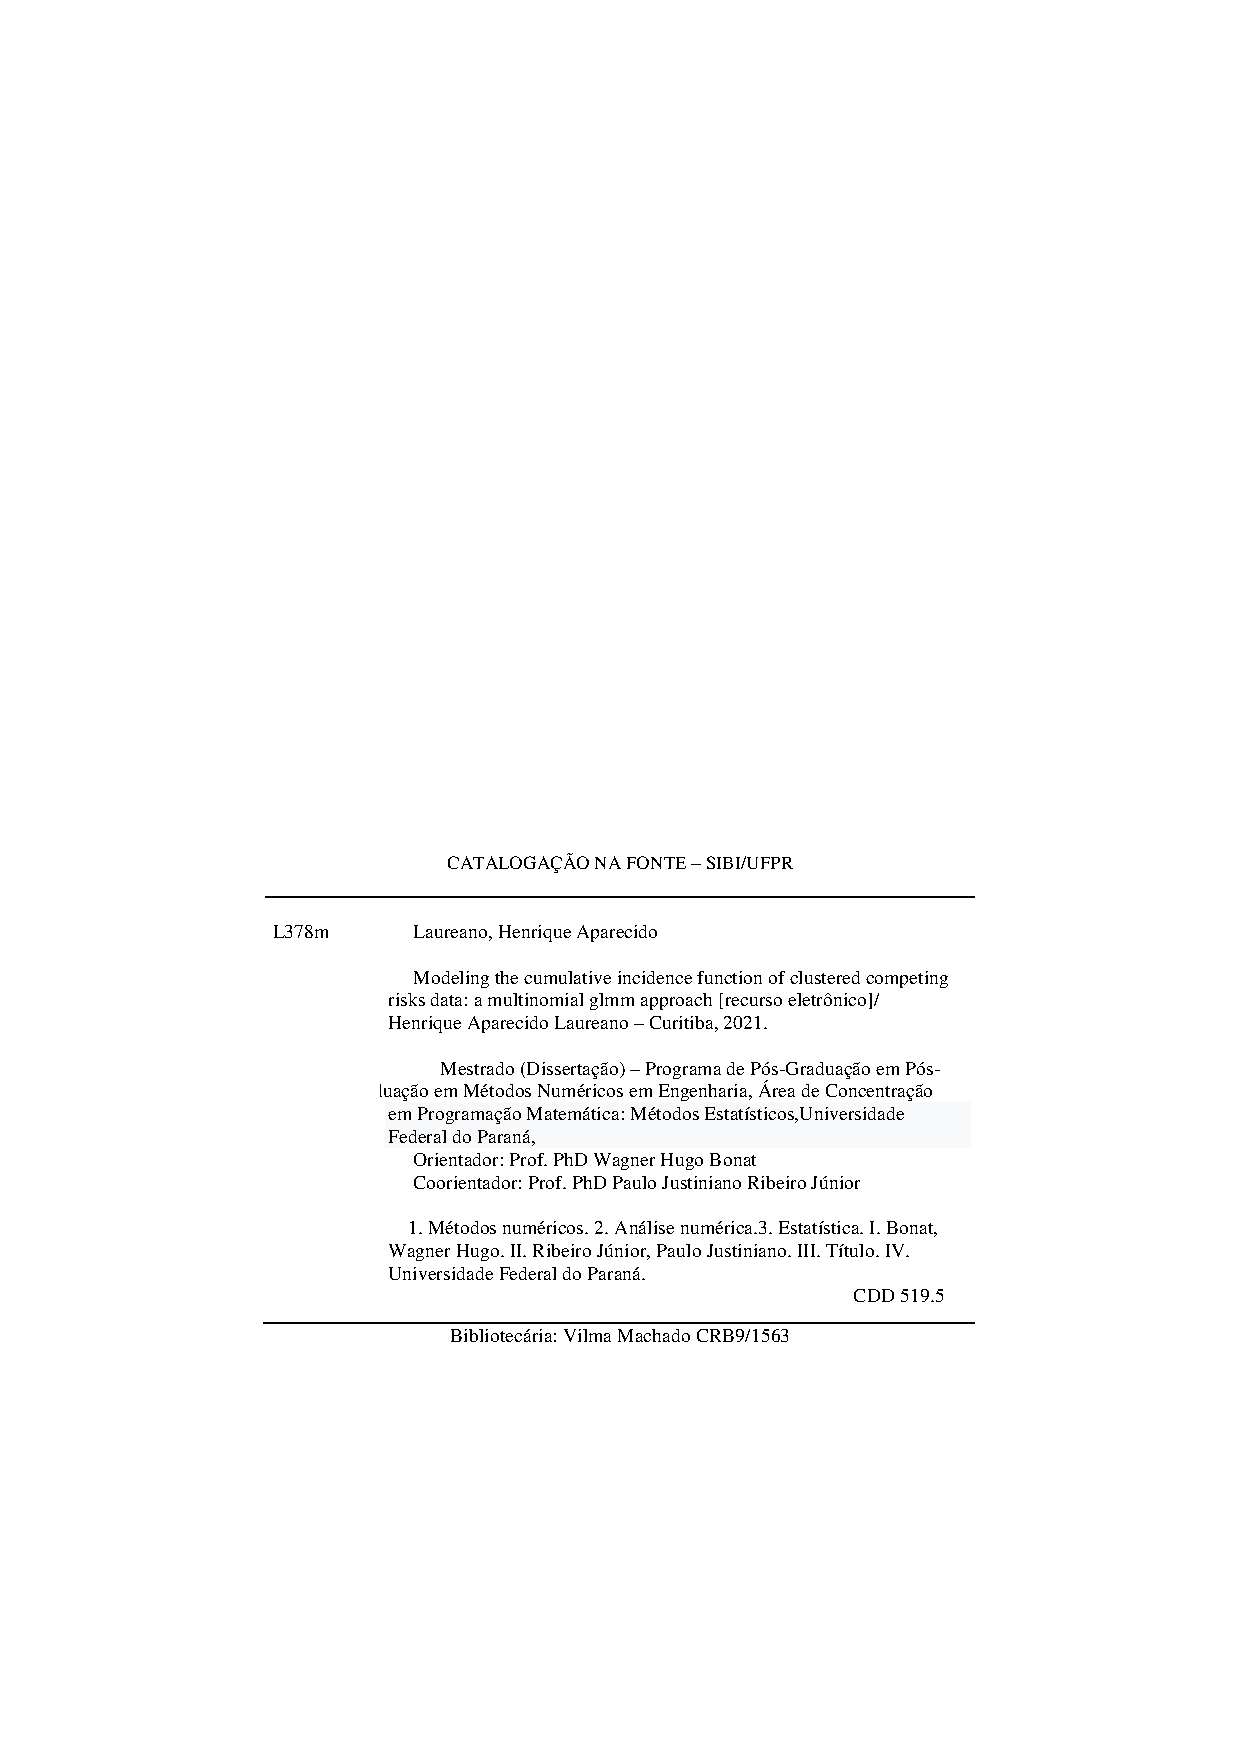
\includepdf{ficha.pdf}
% \end{fichacatalografica}
% ----------------------------------------------------------------------
% inserir folha de aprovação
% \begin{folhadeaprovacao}
%   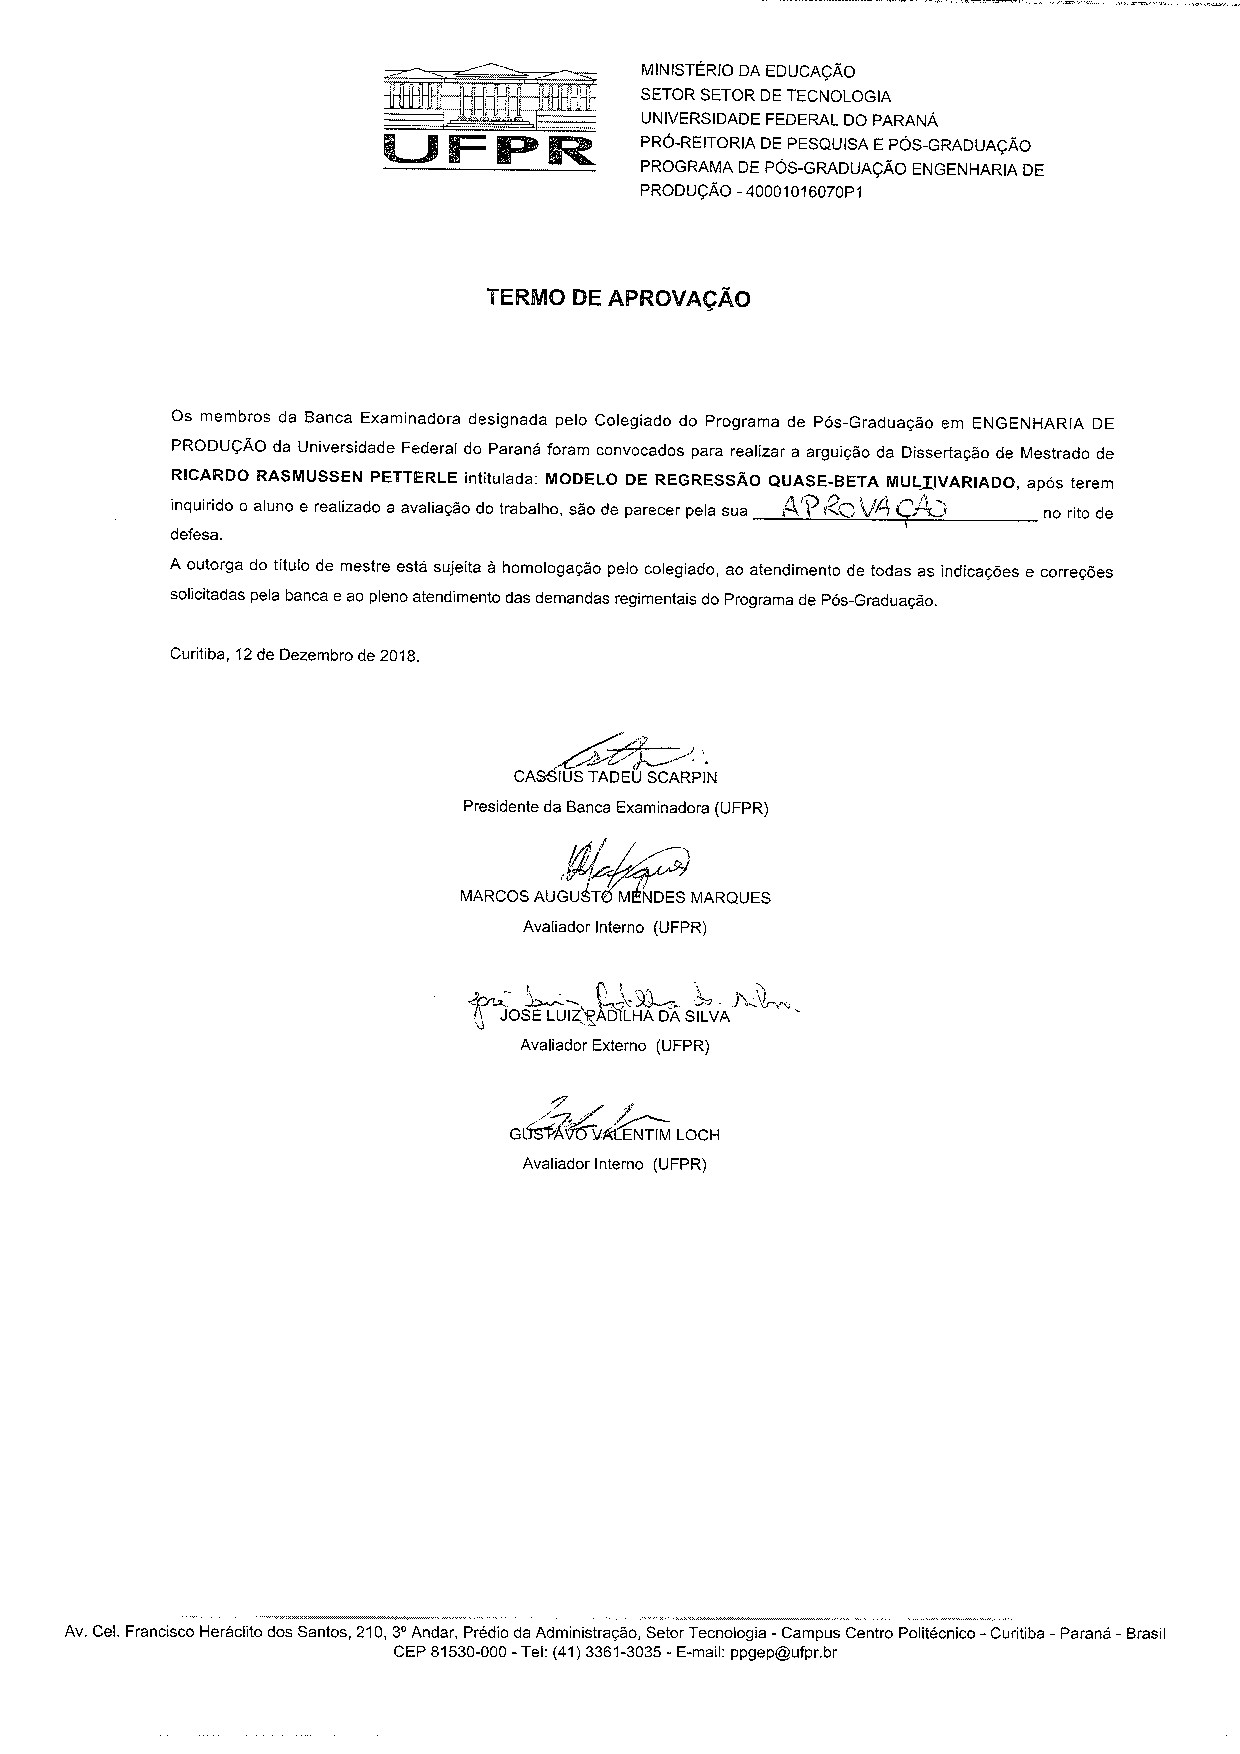
\includepdf{termo.pdf}
% \end{folhadeaprovacao}
\begin{folhadeaprovacao}
 \begin{center}
   {\ABNTEXchapterfont\large\imprimirautor}

   \vspace*{\fill}\vspace*{\fill}
   \begin{center}
     \ABNTEXchapterfont\bfseries\large\imprimirtitulo
   \end{center}
   \vspace*{\fill}

    \hspace{.45\textwidth}
    \begin{minipage}{.5\textwidth}
       \imprimirpreambulo
    \end{minipage}
   \vspace*{\fill}
 \end{center}

 Master thesis approved. XXX XX, 2021.

  \assinatura{\textbf{\imprimirorientador}\\ Supervisor}
  \assinatura{\textbf{Prof. PhD Paulo Justiniano Ribeiro Jr}\\
    Co-supervisor}
  \assinatura{\textbf{Prof. PhD \(\dots\)}\\
    Internal Examinator - PPGMNE}
  \assinatura{\textbf{Prof. PhD \(\dots\)}\\
    Internal Examinator - PPGMNE}
  \assinatura{\textbf{Prof. PhD \(\dots\)}\\External Examiner - }

  \begin{center}
   \vspace*{0.5cm}
   {\large CURITIBA}
   \par
   {\large\imprimirdata}
   \vspace*{1cm}
 \end{center}

\end{folhadeaprovacao}
% ----------------------------------------------------------------------
\begin{dedicatoria}
  \vspace*{22.7cm}
  \begin{flushright}
    \begin{minipage}[H]{4.5cm}
      {To Celita and Olivio}
    \end{minipage}
  \end{flushright}
\end{dedicatoria}
% ----------------------------------------------------------------------
\begin{agradecimentos}
 As Moro once said, I am thankful for everything and everyone.

 Today is the shadow of tomorrow. Today is the present future of
 yesterday. Yesterday is the shadow of today. The wisdom of the past is
 the light of the past. The light of the future casts the shadows of
 tomorrow.
\end{agradecimentos}

\begin{epigrafe}
  \vspace*{\fill}
  \begin{flushright}
    \textit{"It's not supposed to be easy."\\
             (Gregg Popovich)}
              % on Sao Antonio Spurs \(\times\) Oklahoma City Thunder,
              % first game of the 2012 Western Conference Finais
  \end{flushright}
\end{epigrafe}
% ----------------------------------------------------------------------
\newpage
\setlength{\absparsep}{18pt} % ajusta o espaçamento dos parágrafos do
                             % resumo
\setlength{\abstitleskip}{1cm} % adiciona mais um cm após o 'titulo' do
                               % resumo para ficar com 2cm
\begin{resumo}[]
  \vspace{-2cm}
  \begin{center}
    \bfseries{\large{\textsf{ABSTRACT}}}
  \end{center}
  \vspace{0.3cm}

  Clustered competing risks data is a special case of failure time
  data. Besides the cluster structure which implies a within-cluster
  dependence between its elements, this kind of data is characterized by
  1) multiple causes/variables competing to be the one responsible for
  the occurrence of an event, a failure; and 2) censorship, when the
  event of interest happens for none of the competing causes, in the
  study period.

  To handle this type of data, we propose a latent-effects framework, a
  generalized linear mixed model (GLMM), instead of a usual survival
  model. In survival analysis, the modeling is done by means of the
  hazard rate, and the within-cluster dependence accommodation generates
  a complicated likelihood function sometimes intractable. What we do
  here is to model the clustered competing causes in the probability
  scale, in terms of the cumulative incidence function (CIF) of each
  competing cause. In our framework, we suppose a multinomial
  probability distribution for the competing causes and censorship,
  conditioned on the latent effects (within-cluster dependence). The
  latent effects are accommodated by a multivariate Gaussian
  distribution and are modeled by the parameters of its covariance
  matrix. These probability distributions are connected by the CIF,
  modeled here following the specification in \citeonline{SCHEIKE},
  based on the CIF decomposition as the product of an instantaneous risk
  level function with a trajectory time level function. The latent
  effects are inserted in those level functions.  To make the estimation
  of the parameters of this model the most efficient as possible, we use
  the template model builder (TMB) \cite{TMB}. With this R \cite{R21}
  package, we have our log-likelihood function written in C++, we have
  access to state-of-the-art computational libraries, an efficient
  Laplace approximation implementation for the latent-effects, and an
  automatic differentiation (AD) routine, the state-of-the-art in
  derivatives computation. To check the estimability of our model a
  large simulation study is performed, based on different latent
  structure formulations, with the aim to verify which one is most
  adequate. The model presents to be of difficult estimation, with our
  results converging to a latent restructure where the risk and
  trajectory time levels are correlated. In scenarios with high CIF the
  model exhibits good results, but with an excessive variance, showing
  that improvements are necessary.
  
  In scenarios with high CIF the model exhibits good results, but with
  an excessive variance, showing that improvements are necessary.
  
  \textbf{Keywords}: Clustered competing risks.
                     Within-cluster dependence.
                     Multinomial generalized linear mixed model (GLMM).
                     TMB: Template Model Builder.
                     Laplace approximation.
                     Automatic differentiation (AD).
\end{resumo}
% ----------------------------------------------------------------------
\newpage
\setlength{\absparsep}{18pt} % ajusta o espaçamento dos parágrafos do
                             % resumo
\setlength{\abstitleskip}{1cm} % adiciona mais um cm após o 'titulo' do
                               % resumo para ficar com 2cm
\begin{resumo}[]
  \begin{otherlanguage*}{brazil}
    \vspace{-2cm}
    \begin{center}
      \bfseries{\large{\textsf{RESUMO}}}
    \end{center}
    \vspace{0.3cm}

    \textbf{Palavras-chave}: Riscos competitivos agrupados.
                             Depend\^{e}ncia intra-cluster.
                             Modelo linear generalizado misto
                             multinomial (MLGM).
                             TMB: Template Model Builder.
                             Aproxima\c{c}\~{a}o de Laplace.
                             Diferencia\c{c}\~{a}o autom\'{a}tica.
  \end{otherlanguage*}
\end{resumo}
% ----------------------------------------------------------------------
\pdfbookmark[0]{\listfigurename}{lof}
\listoffigures*
\cleardoublepage
% ----------------------------------------------------------------------
%% \pdfbookmark[0]{\listtablename}{lot}
%% \listoftables*
%% \cleardoublepage
% ----------------------------------------------------------------------
\makeatletter
\renewcommand\numberline[1]{
	\leftskip -0.7em
	\rightskip 1.6em
	\parfillskip -\rightskip
	\parindent 0em
	\@tempdima 2.0em
	\vspace{0em}
  \advance\leftskip \@tempdima \null\nobreak\hskip -\leftskip
	ALGORITHM \normalfont #1 ~~ }
\makeatother
% ----------------------------------------------------------------------
\pdfbookmark[0]{\listalgorithmname}{loa}
\listofalgorithms
\cleardoublepage
% ----------------------------------------------------------------------
\makeatletter
\def\numberline#1{\hb@xt@\@tempdima{#1\hfil}}
\makeatother
% ----------------------------------------------------------------------
% \begin{siglas}
% \item[Fig.] Area of the $i^{th}$ component
% \item[456] Isto é um número
% \item[123] Isto é outro número
% \item[lauro cesar] este é o meu nome
% \end{siglas}
% ----------------------------------------------------------------------
% \begin{simbolos}
% \item[\(\mathbb{E}(\cdot)\)] The mathematical expectation of a random
%   variable \(\cdot\)
% \end{simbolos}
% ----------------------------------------------------------------------
\pdfbookmark[0]{\contentsname}{toc}
\tableofcontents*
\cleardoublepage
% ----------------------------------------------------------------------
\makepagestyle{abntheadings}
\makeevenhead{abntheadings}{\ABNTEXfontereduzida\thepage}{}{}
\makeoddhead{abntheadings}{}{}{\ABNTEXfontereduzida\thepage}
\makeheadrule{abntheadings}{\textwidth}{0in}
% ----------------------------------------------------------------------
\textual
% ----------------------------------------------------------------------
\chapter{Introduction}
\label{cap:intro}
Consider a cluster of random variables representing the time until the
occurrence of some event. These random variables are assumed to be
correlated, i.e. for some biological or environmental reason it is not
adequate to assume independence between them. Also, we may be interested
in the occurrence of not only one specific event, having in practice a
competition of events to see which one happens first, if it
happens. Such events may also be of low probability albeit severe
consequences, this is the moment when the cluster correlation makes its
difference: the occurrence of an event in a cluster member should affect
the probability of the same happening in the others.

A realistic context that fits perfectly with the framework described
above is the study of disease incidence in family members, where each
member is indexed by a random variable and each cluster consists of a
familiar structure. More specifically, we are interested in what is
called \textit{family studies}. Besides the dependence between family
members, this kind of data is characterized by being consisted of big
samples, or even a population, and having a lot of clusters/families of
small size. The inspiration to these kinds of problems came from the
work developed in \citeonline{SCHEIKE}, where they studied breast cancer
incidence in mothers and daughters but using a nontrivial estimation
framework. Based on that, the aim of this thesis is to propose a simpler
estimation framework taking advantage of several \textit{state-of-art}
computational libraries and see how far we can go in several
scenarios. Until now we have just contextualized, we still need to
introduce the methodology. To do this, some definitions and theoretical
contexts are welcome.

When the object under study is a random variable representing the time
until some event occurs, we are in the field of \textit{failure time
data} \cite{kalb&prentice}. The occurrence of an event is generally
denoted \textit{failure}, and major areas of application are biomedical
studies and industrial life testing. In this thesis, we maintain our
focus on the former. As common in science, same methodologies can
receive different names depending on the area. In industrial life
testing is performed what is called a \textit{reliability analysis}; in
biomedical studies is performed what is called
\textit{survival analysis}. Generally, the term \textit{survival} is
applied when we are interested in the occurrence of only one event, a
\textit{failure time process}. When we are interested in the occurrence
of more than one event we enter in the yard of \textit{competing risks}
and \textit{multistate} models. A visual aid is presented on
\autoref{fig:intro1} and a comprehensive reference is
\citeonline{kalb&prentice}.

Failure time and competing risks processes may be seen as particular
cases of a multistate model. Besides the number of events (states) of
interest, the main difference between a multistate model and its
particular cases is that only in the multistate scenario we may have
transient states, using a \textit{stochastic process} language. In the
particular cases, all states besides the initial state 0, are absorbents
- once you reached it you do not leave. The simplest multistate model
that exemplify this behavior is the illness-death model,
\autoref{fig:intro1}~C), where a patient (initially in state 0) can get
sick (state 1) or die (state 2); if sick it can recover (returns to
state 0) or die. We work in this thesis only with competing risks
processes, and for each patient we need the time (age) until the
occurrence, or not, of the event.

\begin{figure}[H]
 \setlength{\abovecaptionskip}{.0001pt}
 \caption{ILLUSTRATION OF MULTISTATE MODELS FOR A A) FAILURE TIME
          PROCESS; B) COMPETING RISKS PROCESS; AND C) ILNESS-DEATH
          MODEL, THE SIMPLEST MULTISTATE MODEL}
 \vspace{0.5cm}\centering
 \tikzfig{fig1}\\
 \vspace{0.5cm}
 \begin{footnotesize}
  SOURCE: The author~(2021).
 \end{footnotesize}
 \label{fig:intro1}
\end{figure}

When for some known or unknown reason we are not able to see the
occurrence of an event, we have what is denoted \textit{censorship}.
Still in the illness-death model, during the period of follow up the
patient may not get sick or die, staying at state 0. This is denoted
\textit{right-censorship}; if a patient is in state 1 at the end of the
study, we are \textit{censored} to see him reaching the state 2 or
returning to state 0. This is the inherent idea to censorship and must
be present in the modeling framework, thus arriving in the so-called
\textit{survival models} \cite{kalb&prentice}.

A survival model deals with the survival experience. Usually, the
survival experience is modeled in the \textit{hazard} (failure rate)
scale and it can be expressed for a subject \(i\) as
\begin{equation}
  \lambda(t \mid \bm{x}_{i}) =
  \lambda_{0}(t) \times c(\bm{x}_{i} \bm{\beta})
  \quad \text{at time}~t,
  \label{eq:intro1}
\end{equation}
i.e. as the product of an arbitrary baseline hazard function
\(\lambda_{0}(\cdot)\), with a specific function form \(c(\cdot)\), that
will depend on the probability distribution to be chosen for the failure
time and on predictors/covariates/explanatory/independent variables
\(\bm{x}_{i} = [x_{1}~\dots~x_{p}]\), where \(\bm{\beta}^{\top} =
[\beta_{1}~\dots~\beta_{p}]\) is the parameters vector.

This structure is specified for a failure time process, as in
\autoref{fig:intro1}~A). Nevertheless, the idea is easy to extend. We
basically have the \autoref{eq:intro1}'s model to each cause-specific
(in a competing risks process) or transition (in a multistate process).
For competing risks, the probable most famous approach is the
\citeonline{fine&gray} subdistribution model. A complete and extensive
detailing can be, again, found in \citeonline{kalb&prentice}.

In this work we approach the case of clustered competing risks. Besides
the cause-specific structure, we have to deal with the fact that the
events are happening in related individuals. This configures what is
denoted \textit{family studies}, i.e. we have a cluster/group/family
dependence that needs to be considered, accommodated, and modeled. This,
possible, dependence is something that we do not actually measure but
know (or just suppose) that exists. In the statistical modeling language
this characteristic receives the name of \textit{random} or
\textit{latent effect}.

A survival model with a latent effect, association, or unobserved
heterogeneity, is denoted \textit{frailty model}
\cite{frailty78,frailty79,liang95,petersen98}. In its simplest form, a
frailty is an unobserved random proportionality factor that modifies the
hazard function of an individual, or of related individuals. Frailty
models are extensions of \autoref{eq:intro1}'s model, and its use
implies challengeable likelihood functions (statistical objective
functions) and inference routines done via elaborated and slow
expectation–maximization (EM) algorithms \cite{nielsen92,klein92} or
inefficient Markov chain Monte Carlo (MCMC) schemes \cite{hougaard00}.
With multiple survival experiences, the general idea is the same but
with even more challengeable likelihoods
\cite{prentice78,larson85,kuk92,therneau00}.

In the competing risks setting, the hazard scale (focusing on the
cause-specific hazard) is not the only possible scale to work on. A more
attractive possibility is to work on the probability scale
\cite{andersen12}, focusing on the cause-specific cumulative incidence
function (CIF). Besides the within-family dependence, in family studies
there is often a strong interest in describing age at disease onset,
which is directly described by the cause-specific CIF. The CIF is the
cumulative probability of experiencing a failure by a given competing
cause along the time. Therefore, making the probability scale a more
attractive and logical choice. Since the CIF plays a central role in
this master thesis, it will be formally defined later in a place with
greater emphasis.

Besides the CIF specification itself, the known works with clustered
competing risks data in the probability scale, differ in terms of
likelihood construction and parameters estimation routines. There is a
lack of methodology predominance in the literature, but with its
majority being designed for bivariate CIFs, where increasing the CIF's
dimension is a limitation. Some of the existing options are
\begin{itemize}
 \item Nonparametric approaches \cite{cheng07,cheng09};
 \item Linear transformation models \cite{fine99,gerds12};
 \item Semiparametric approaches based on
  \begin{itemize}
   \item Composite likelihoods \cite{shih,SCHEIKE};
   \item Estimating equations \cite{cheng&fine12,crossoddsratioSCHEIKE};
   \item Copula models \cite{semiparametricSCHEIKE};
   \item Mixture models \cite{naskar05,shi13}.
  \end{itemize}
\end{itemize}

With the definitions and the theoretical context being made, let us be
more specific. To work with competing risks data on the probability
scale plus a latent structure allowing for within-cluster dependence of
both risk and timing, \citeonline{SCHEIKE} proposed a pairwise composite
likelihood approach based on the factorization of the cause-specific CIF
as the product of a cluster-specific risk level function with a
cluster-specific failure time trajectory function. A composite approach
\cite{lindsay88, cox&reid04, varin11} is a valid alternative to a full
likelihood analysis in high-dimensional situations when a full approach
is too computational costly or even inviable. A clear advantage of this
approach is that we do not need to care about a joint distribution
specification, which generally translates also into a computational
advantage. A disadvantage is the likelihood function specification,
which becomes much more challengeable, besides the number of small
details to workaround from the fact of being working with not an exact
likelihood function.

We do not have any guarantees that a full likelihood inference procedure
is not viable here, so we try to reach the same goal of
\citeonline{SCHEIKE} albeit with a simpler maximum likelihood estimation
framework taking advantage of \textit{state-of-art} software, something
still not so common in the statistical modeling community. This simpler
framework is based on a generalized linear mixed model (GLMM). Instead
of concentrating on failure time data and consequently having a
survival/frailty model based on the hazard scale, or using a composite
approach (or any other of the options listed above), we just build the
joint/full likelihood function (a multinomial model with its link
function based on the cluster-specific CIF, accouting for an appropriate
latent effects structure), marginalize (integrate out the latent
effects) and optimize it. A Fisherian approach per se.

In a standard linear model we assume that the response
variable \(Y_{i}\), conditioned on the covariates \(\bm{x}_{i}\),
follows a normal/Gaussian distribution and what we do is to model its
mean, \(\mu_{i} \equiv \mathbb{E}(Y_{i} \mid \bm{x}_{i})\), via a linear
combination. As much well explained in \citeonline{GLM72}, with the aid
of a \textit{link function} \(g(\cdot)\), this idea is generalized to
distributions of the \textit{exponential family}. Many of its members
are useful for practical modelling, such as the Poisson (for counting
data), binomial (dichotomic data), gamma (continuous but positive) and
Gaussian (continuous data) distributions. This extended framework
received the name of generalized linear models (GLMs) \cite{GLM72}, and
is probably the most popular statistical modelling framework. A
comprehensive reference is \citeonline{GLM89}.

 Despite its flexibility, the GLMs are not suitable for dependent
data. For the analysis of such data, \citeonline{laird82} proposed the
random effects regression models for longitudinal/repeated-measures data
analysis. \citeonline{breslow93} presented the GLMMs for the analysis of
non-Gaussian outcomes. What makes a GLM into a GLMM is the addition of a
latent effect \(\bm{u}\) (then, \textit{m}ixed) into the mean
structure. The mean structure of a standard GLMM for a subject \(i\) is
defined as
\[
  g(\mu_{i}) = \bm{x}_{i}\bm{\beta} + \bm{z}_{i}\bm{u},
  \quad \bm{u} \sim \text{Multivariate Normal}(\bm{0},\bm{\Sigma})
\]
where the latent effect is assumed to follow a multivariate Gaussian
distribution of zero mean and a parametrized variance-covariance matrix
\(\bm{\Sigma}\). Its correct linkage to the mean structure is made
through the \(i^\text{th}\) vector row of a design-matrix \(\bm{Z}\).
The covariates are into \(\bm{x}_{i}\), the \(i^\text{th}\) vector row
of a model-matrix \(\bm{X}\), with \(\bm{\beta}\) being a vector of
unknown parameters.

In the GLMM framework \cite{GLMM}, we can accommodate all competing
causes of failure and censorship with a multinomial probability
distribution, easily extend to any number of competing causes. The
within-cluster dependence is accommodated via the latent effect and the
cause-specific CIFs via the model's link function. The estimation and
inference are done via an efficient implementation and state-of-art
computational libraries provided through the R \cite{R21} package
TMB \cite{TMB}. The latent effects are handled out by means of an
efficient Laplace approximation \cite{corestats,patrao} and automatic
differentiation (AD)
\cite{corestats,peyre} routines.

\section{GOALS}

\subsection{General goals}

Propose and evaluate a maximum likelihood estimation approach of a
multinomial generalized linear mixed model (multiGLMM) to the cluster
and cause-specific cumulative incidence function (CIF) of clustered
competing risks data.

\subsection{Specific goals}

\begin{enumerate}
 \item Simulate from the model, i.e. generate synthetic data to study
       statistical properties.

 \item Write the model in the Template Model Builder (TMB) software,
       developed by \citeonline{TMB} and possibly the most efficient
       likelihood-based way of doing such task.

 \item Take advantage of TMB's functionalities with special attention to
       the computation of gradients and Hessians via a
       \textit{state-of-art} automatic differentiation (AD)
       implementation; and a joint likelihood marginalization via an
       efficient Laplace approximation routine.

 \item Assess the maximum likelihood estimation method embedded on TMB.
       Check its properties in our model for different complexity level
       in terms of parametric space and latent effect structures.

 \item Make exact likelihood-based inference to the cluster and
       cause-specific CIF of clustered competing risks data.
\end{enumerate}

\section{JUSTIFICATION}

In the biomedical statistical modeling literature, the study of disease
occurrence in related individuals receives the name of family studies.
Key points of interest are the within-family dependence and determining
the role of different risk factors. The within-family dependence may
reflect both disease heritability and the impact of shared environmental
effects. The role of different risk factors arrives in the class of
multivariate models, which options are limited in the statistical
literature. Thus, the number of statistical models for competing risks
data that accommodate the within-cluster/family dependence is even more
limited. Some modeling options are briefly commented in
\citeonline{SCHEIKE}, with his pairwise composite approach being
proposed as a new and better option to model the cause-specific
cumulative incidence function (CIF), describing age at disease onset, of
clustered competing risks data on the probability scale. We propose to
model the cause-specific CIF and accommodate the within-family
dependence in the same fashion (via a latent structure that allows the
absolute risk and the failure time distribution to vary between
families) but with an easier estimation framework, based on a
full-likelihood approach of a multinomial generalized linear mixed
model.

\section{LIMITATION}

This work restraint to the proposition and maximum likelihood estimation
method evaluation of a multinomial model for the cause-specific
cumulative incidence function (CIF) of competing risks data in the
context of family studies, with a latent effect structure to accommodate
within-family dependence with regard to both risk and timing. Family
studies are characterized by a considerable amount of clusters
(families) but with each one having a small number of elements. Given
its considerable model complexity, hypothesis tests; residual analysis;
and good-of-fit measures are not contemplated.

\section{THESIS ORGANIZATION}

This master thesis contains 6 chapters including this introduction.
\autoref{cap:methods} presents a systematic review of the main aspects
involved in the formulation, optimization, and implementation of a
generalized linear mixed model (GLMM). Given the modeling framework
overview, \autoref{cap:model} presents our multinomial GLMM (multiGLMM)
to model the cause-specific cumulative incidence function (CIF) of
clustered competing risks data. In \autoref{cap:datasets} we describe
the simulation procedure to generate synthetic data and present some
model particularities. In \autoref{cap:results} the obtained results are
presented, and in \autoref{cap:finalc} we discuss the contributions of
this thesis and present some suggestions for future work.

% END ==================================================================

% ----------------------------------------------------------------------
\chapter{Generalized linear mixed models: formulation, optimization, and
  implementation}
\label{cap:methods}
This chapter presents a systematic review of the main theoretical
aspects involved in the construction, estimation and implementation of a
generalized linear mixed model (GLMM). We start in \autoref{cap:joint}
with the model construction framework, concluding with the so-called
joint likelihood function. \autoref{cap:laplace} address the
marginalization of that joint likelihood, performed here in terms of a
Laplace approximation technique. \autoref{cap:opt} discusses available
alternatives for the parameters optimization of the marginal likelihood
obtained through that marginalization. \autoref{cap:ad} talks about
automatic differentiation (AD), the most efficent manner of computing
derivatives, and a key point for us. Last but not least, in
\autoref{cap:tmb} we present the computational tool used to peform all
the discussed procedure, the TMB: Template Model Builder. A very
exciting \texttt{R} \cite{R18} package developed by~\citeonline{TMB}.

\section{CONSTRUCTION: JOINT LIKELIHOOD FUNCTION}
\label{cap:joint}

A GLMM models an \(n\)-vector of exponential family random variables,
\(\mathbf{Y}\), in terms of its conditional expected value, \(\bm{\mu}
\equiv \mathbb{E}(\mathbf{Y} \mid \bm{x}, \mathbf{u})\), via a
linear combination called of linear predictor and generally expressed by
\begin{equation}
  g(\bm{\mu}) = \bm{x} \bm{\beta} + \mathbf{Zu}, \quad
  \mathbf{u} \sim \mathcal{N}(\mathbf{0}, \bm{\Sigma}).
  \label{eq:gmu}
\end{equation}
In other words, a GLMM is a generalized linear model (GLM) in which the
linear predictor depends on some Gaussian latent effects,
\(\mathbf{u}\), times a latent effects model matrix \(\mathbf{Z}\).
Since we do not observe the latent component, an exemplification of the
idea embedded in matrix \(\mathbf{Z}\) is welcome. Suppose, e.g. three
individuals (or clusters) and that each one has two measures. This
configures a repeated measures context, the most common latent structure
in family studies.. Also, it is reasonable to admit that each individual
has its particular latent effect value. Consequently,
\[
  \mathbf{Zu} = \begin{bmatrix}
                 1 & 0 & 0\\1 & 0 & 0\\
                 0 & 1 & 0\\0 & 1 & 0\\
                 0 & 0 & 1\\0 & 0 & 1\\
                \end{bmatrix} \begin{bmatrix}
                               u_{1}\\u_{2}\\u_{3}\\
                              \end{bmatrix} = \begin{bmatrix}
                                               u_{1}\\u_{1}\\
                                               u_{2}\\u_{2}\\
                                               u_{3}\\u_{3}\\
                                              \end{bmatrix},
\]
where \(\mathbf{u}^{\top} = [u_{1}~u_{2}~u_{3}]\) and \(\mathbf{Z}\) has
the role of projecting the values of \(\mathbf{u}\) to match the number
of measures.

In a mixed model the mean structure is approached into a combination of
probability distributions. It is a combination since we have to assume
probabilistic structures for the observed and non-observed (latent)
data. To each observed variable \(y_{ij}\) we have a probability
distribution of the exponential family, denoted by \(f(y_{ij} \mid
\mathbf{u}_{i}, \bm{\theta})\). To the non-observed latent effect we
have, generally, a (multivariate) Gaussian distribution, denoted by
\(f(\mathbf{u}_{i} \mid \bm{\Sigma})\). To each individual or unity
under study, \(i\), and to each measure, \(j\), we have the product of
these probability densities, a likelihood contribution.

Our goal is to estimate the parameter vector \(\bm{\theta} =
[\bm{\beta}~\bm{\Sigma}]^{\top}\) of a mean structure, as in
\autoref{eq:gmu}. Besides the role of emphasizing the fact that
\(\bm{\mu}\) is a function of \(\bm{\theta}\) and that we want to
estimate that \(\bm{\theta}\), the likelihood function ties the
probability densities. i.e. the likelihood is the product of the product
of probability densities, to each subject \(i\). Since \(Y_{i}\) are
mutually independent, the likelihood for \(\bm{\theta}\) can be written
as
\begin{equation}
  L(\bm{\theta} \mid \mathbf{y}, \mathbf{u}) =
  \prod_{i=1}^{I}~\prod_{j=1}^{n_{i}}~
  f(y_{ij} \mid \mathbf{u}_{i}, \bm{\beta}, \bm{\Sigma})~
  f(\mathbf{u}_{i} \mid \bm{\Sigma}).
  \label{eq:joint}
\end{equation}
From standard probability theory is easy to see that in the right-hand
side (r.h.s.) we have a joint density, consequently, \autoref{eq:joint}
represents what is called a joint likelihood function. What makes
problematic working with this joint likelihood is that we do not have
all the necessary information to just maximize it and get the desired
parameter estimates. The latent effect \(\mathbf{u}\) is
\textit{latent}, i.e. we do not observe it. To handle this we have
basically two available paths.

\section{MARGINALIZATION: LAPLACE APPROXIMATION}
\label{cap:laplace}

To deal with a joint likelihood function as in \autoref{eq:joint} we
have a choice to make. Be or not to be Bayesian. Each choice has its own
difficulties, advantages, and characteristics.

The Bayesian path assumes that all \(\bm{\theta}\) components are random
variables. With all parameters being treated as random variables and,
since we do not observe them, what the Bayesian framework does is try to
compute the mode of each ``parameter'' marginal distribution, generally,
via a sampling algorithm called MCMC: Markov chain Monte Carlo
\cite{MCMC, Diaconis}. The advantage of being Bayesian is that we can
reach an MCMC algorithm to basically any statistical model, the
disadvantage is that this approach is very time consuming and we have to
propose prior distributions to each ``parameter''. These prior proposals
are not always easy to make and, the resulting marginal distributions
can be very depending of it.

A Bayesian approach can be applied in basically any context, without
guarantees that will work - obtain convergence to all parameters is not
a straightforward task. However, in complex scenarios they can be the
only available method to ``maximize'' the likelihood function. This is
not the case here. We have a joint density where one of the random
variables is not observed, but we are not interested in it, only in the
variance parameters inherent in it. Again, from standard probability
theory, if we have a joint density we can just integrate out the
undesired variable resulting in
\begin{equation}
  \begin{aligned}
    L(\bm{\theta} \mid \mathbf{y}) &=
    \prod_{i=1}^{I}~\int_{\mathcal{R}^{\mathbf{u}_{i}}}
    \left[
      ~\prod_{j=1}^{n_{i}}~
      f(y_{ij} \mid \mathbf{u}_{i}, \bm{\beta}, \bm{\Sigma})~
      f(\mathbf{u}_{i} \mid \bm{\Sigma})
    \right]\text{d} \mathbf{u}_{i}\\
    &= \prod_{i=1}^{I}~\int_{\mathcal{R}^{\mathbf{u}_{i}}}~
    f(\mathbf{y}_{i}, \mathbf{u}_{i} \mid \bm{\theta})~
    \text{d} \mathbf{u}_{i},
    \label{eq:generalmarginal}
  \end{aligned}
\end{equation}
a marginal density that keeps the parameters \(\bm{\Sigma}\) of the
integrated variable.

When the response distribution of a mixed model is Gaussian, is
analytically tractable to integrate \(\mathbf{u}\) out of the joint
density. Consequently, it is possible to evaluate the marginal
likelihood exactly. This is the case of the linear mixed models (LMMs)
and the main difference to the GLMMs. When the response distribution is
not Gaussian, generally, it is not anymore analytically tractable to
integrate out the latent effect. So what do we do? Well, we have
basically two options.

We can avoid the integrals in \autoref{eq:generalmarginal} replacing it
by integrals that are more analytically tractable. This can be performed
via an algorithm called Expectation-Maximization (EM) proposed by
\citeonline{EM77}. This approach is considered a little bit naive and
generally is not recommended if you have a better option. The other
option consists of performing a numerical integration, i.e.
approximating the integral. The most common way of doing that in the
statistical modeling literature is via an adaptive Gaussian quadrature
rule \cite{quadrature}. In general, adaptive Gaussian quadratures are
not so simple of using (may be unstable, computationally expensive and
we have the problem of choosing how many integration points should be
used). To us, the better option consists in take advantage of the
exponential family structure and the fact that we are dealing with
Gaussian latent effects. These ideas converge to an adaptive Gaussian
quadrature with one integration point, also called as \textit{Laplace
  approximation} \cite{molenberghs&verbeke, LA4H, tierney, corestats}.

With an integral that is analytically intractable, we may approximate it
to obtain a tractable closed-form expression allowing then the numerical
maximization of the resulting marginal likelihood function
\cite{patrao}. The Laplace approximation has been designed to
approximate integrals in the form
\begin{equation}
  \int_{\mathcal{R}^{\mathbf{u}_{i}}}
  \exp\{Q(\mathbf{u}_{i})\} \text{d} \mathbf{u}_{i}\approx
  (2\pi)^{n_{\mathbf{u}}/2}~
  |{Q}''(\mathbf{\hat{u}}_{i})|^{-1/2}~\exp\{Q(\mathbf{\hat{u}}_{i})\},
  \label{eq:laplace}
\end{equation}
where \(Q(\mathbf{u}_{i})\) is a known, unimodal bounded function and
\(\mathbf{\hat{u}}_{i}\) is the value for which \(Q(\mathbf{u}_{i})\) is
maximized. As \citeonline{corestats} shows, a Laplace approximation
consists of a second order Taylor expansion of \(\log f(\mathbf{y}_{i},
\mathbf{u}_{i} \mid \bm{\theta})\), about \(\mathbf{\hat{u}}_{i}\), that
gives
\[
  \log f(\mathbf{y}_{i}, \mathbf{u}_{i} \mid \bm{\theta})\approx
  \log f(\mathbf{y}_{i}, \mathbf{\hat{u}}_{i} \mid \bm{\theta}) -
  \frac{1}{2}
  (\mathbf{u}_{i} - \mathbf{\hat{u}}_{i})^{\top}\mathbf{H}~
  (\mathbf{u}_{i} - \mathbf{\hat{u}}_{i}),
\]
where \(\mathbf{H} = - \nabla_{u}^{2} \log f(\mathbf{y}_{i},
\mathbf{\hat{u}}_{i} \mid \bm{\theta})\). Hence, we can approximate the
joint by
\begin{equation}
  f(\mathbf{y}_{i}, \mathbf{u}_{i} \mid \bm{\theta})\approx
  f(\mathbf{y}_{i}, \mathbf{\hat{u}}_{i} \mid \bm{\theta})~\exp
  \left\{- \frac{1}{2}
    (\mathbf{u}_{i} - \mathbf{\hat{u}}_{i})^{\top}\mathbf{H}~
    (\mathbf{u}_{i} - \mathbf{\hat{u}}_{i})
  \right\}.
  \label{eq:taylor}
\end{equation}
From here we start to take advantage of the points mentioned above.
First, the fact that we are dealing with Gaussian distributed latent
effects. In \autoref{eq:taylor} we have the core of a Gaussian density,
that complete is
\[
  \int_{\mathcal{R}^{\mathbf{u}_{i}}}
  \frac{1}{(2\pi)^{n_{\mathbf{u}}/2}~|\mathbf{H}^{-1}|^{1/2}}~\exp
  \left\{- \frac{1}{2}
    (\mathbf{u}_{i} - \mathbf{\hat{u}}_{i})^{\top}\mathbf{H}~
    (\mathbf{u}_{i} - \mathbf{\hat{u}}_{i})
  \right\} \text{d}\mathbf{u}_{i} = 1,
\]
i.e. integrates to 1. Integrating \autoref{eq:taylor} follows that
\begin{align*}
  \int_{\mathcal{R}^{\mathbf{u}_{i}}}
  f(\mathbf{y}_{i}, \mathbf{u}_{i} \mid \bm{\theta})
  ~\text{d}\mathbf{u}_{i}
  &\approx f(\mathbf{y}_{i}, \mathbf{\hat{u}}_{i} \mid \bm{\theta})
    \int_{\mathcal{R}^{\mathbf{u}_{i}}} \exp
    \left\{- \frac{1}{2}
    (\mathbf{u}_{i} - \mathbf{\hat{u}}_{i})^{\top}\mathbf{H}~
    (\mathbf{u}_{i} - \mathbf{\hat{u}}_{i})
    \right\} \text{d}\mathbf{u}_{i}\\
  &= (2\pi)^{n_{\mathbf{u}}/2}~|\mathbf{H}|^{-1/2}~
    f(\mathbf{y}_{i}, \mathbf{\hat{u}}_{i} \mid \bm{\theta}),
\end{align*}
i.e. we get \autoref{eq:laplace}, a first order Laplace approximation to
the integral. Careful accounting of the approximation error shows it to
generally be \(\mathcal{O}(n^{-1})\), where \(n\) is the sample size and
assuming a fixed length for \(\mathbf{u}_{i}\) \cite{corestats}.

The second advantage of a Laplace approximation approach in a GLMM is
the exponential family structure. In a usual GLMM, the response follows
a one-parameter exponential family distribution that can be written as
\[
  f(\mathbf{y}_{i} \mid \mathbf{u}_{i}, \bm{\theta}) = \exp
  \left\{\mathbf{y}_{i}^{\top}
    (\bm{x}_{i}\bm{\beta} + \mathbf{Z}_{i}\mathbf{u}_{i}) -
    \mathbf{1}_{i}^{\top}
    b(\bm{x}_{i}\bm{\beta} + \mathbf{Z}_{i}\mathbf{u}_{i}) +
    \mathbf{1}_{i}^{\top} c(\mathbf{y}_{i})
  \right\},
\]
where \(b(\cdot)\) and \(c(\cdot)\) are known functions. This general
and easy to compute expression, together with a (multivariate) Gaussian
distribution, highlights the convenience of the Laplace method. The
\(Q(\mathbf{u}_{i})\) function to be maximized can be expressed as
\begin{equation}
  \begin{aligned}
    Q(\mathbf{u}_{i}) &= \mathbf{y}_{i}^{\top}
    (\bm{x}_{i}\bm{\beta} + \mathbf{Z}_{i}\mathbf{u}_{i}) -
    \mathbf{1}_{i}^{\top}
    b(\bm{x}_{i}\bm{\beta} + \mathbf{Z}_{i}\mathbf{u}_{i}) +
    \mathbf{1}_{i}^{\top} c(\mathbf{y}_{i})\\
    &- \frac{n_{\mathbf{u}}}{2} \log (2\pi) -
    \frac{1}{2} \log |\bm{\Sigma}| -
    \frac{1}{2} \mathbf{u}_{i}^{\top}\bm{\Sigma}^{-1}~\mathbf{u}_{i}.
  \end{aligned}
\end{equation}
The approximation in~\autoref{eq:laplace} requires the maximum
\(\mathbf{\hat{u}}_{i}\) of the function \(Q(\mathbf{u}_{i})\). As we
assume a Gaussian distribution with a known mean for the latent effects,
we have the perfect initial guess for a gradient-based maximization
method as the Newton-Raphson (NR) algorithm. The NR method consists of
an iterative scheme as follows:
\[
  \mathbf{u}_{i}^{(k+1)} = \mathbf{u}_{i}^{(k)} -
  {Q}''(\mathbf{u}_{i}^{(k)})^{-1}~{Q}'(\mathbf{u}_{i}^{(k)}),
  \quad k = 0,~1,~\dots
\]
until convergence, which gives \(\mathbf{\hat{u}}_{i}\). At this stage,
all parameters \(\bm{\theta}\) are considered known. \citeonline{patrao}
presents the generic expressions for the derivatives required by the NR
method, given by the following:
\begin{equation}
  \begin{aligned}
    {Q}'(\mathbf{u}_{i}^{(k)}) &= \{\mathbf{y}_{i} -
    {b}'(\bm{x}_{i}\bm{\beta} +
    \mathbf{Z}_{i}\mathbf{u}_{i}^{(k)})\}^{\top} -
    {\mathbf{u}_{i}^{(k)}}^{\top} \bm{\Sigma}^{-1},\\
    {Q}''(\mathbf{u}_{i}^{(k)}) &=
    - \text{diag}\{{b}''(\bm{x}_{i}\bm{\beta} +
    \mathbf{Z}_{i}\mathbf{u}_{i}^{(k)})\} - \bm{\Sigma}^{-1}.
  \end{aligned}
  \nonumber
\end{equation}
At \(k = 0\) we have the initial guess.

Finally, the marginal log-likelihood function returned by the Laplace
approximation, to each invividual or unit under study \(i\), is as
follows:
\begin{equation}
  \begin{aligned}
    l(\bm{\theta} \mid \mathbf{y}_{i}) =
    \log L(\bm{\theta} \mid \mathbf{y}_{i}) &=
    \frac{n}{2} \log (2\pi) - \frac{1}{2} \log
    \left|
      \text{diag}\{{b}''(\bm{x}_{i}\bm{\beta} +
      \mathbf{Z}_{i}\mathbf{\hat{u}}_{i})\} + \bm{\Sigma}^{-1}
    \right|\\
    &+ \mathbf{y}_{i}^{\top}
    (\bm{x}_{i}\bm{\beta} + \mathbf{Z}_{i}\mathbf{\hat{u}}_{i}) -
    \mathbf{1}_{i}^{\top}
    b(\bm{x}_{i}\bm{\beta} + \mathbf{Z}_{i}\mathbf{\hat{u}}_{i}) +
    \mathbf{1}_{i}^{\top} c(\mathbf{y}_{i})\\
    &- \frac{n_{\mathbf{u}}}{2} \log (2\pi) -
    \frac{1}{2} \log |\bm{\Sigma}| - \frac{1}{2}
    \mathbf{\hat{u}}_{i}^{\top}\bm{\Sigma}^{-1}~\mathbf{\hat{u}}_{i},
  \end{aligned}
  \nonumber
\end{equation}
that can now be numerically maximized over the model parameters
\(\bm{\theta} = [\bm{\beta}~\bm{\Sigma}]^{\top}\).

\section{OPTIMIZATION: MARGINAL LIKELIHOOD FUNCTION}
\label{cap:opt}

At this point it is already clear that we have two optimizations to be
performed, an ``inside'' and an ``outside'' optimization. The inside one
is made into the Laplace approximation layer via a Newton-Raphson
algorithm, a Newton's method. The outside optimization is made with the
Laplace approximation outputs, i.e. the maximization step
\autoref{eq:generalmarginal}'s marginal log-likelihood over its
parameters \(\bm{\theta}\). This task is usually performed via a
quasi-Newton method, we focus on two of the most traditional ones: the
Broyden-Fletcher-Goldfarb-Shanno (BFGS) algorithm and the PORT routines.

The inside optimization is the numerical maximization of the joint
log-likelihood w.r.t. its latent effects. This is kind of a simple task
since all model parameters are considered as fixed and we ``know'' that
the latent effects are distributed with zero mean, i.e. we have the
perfect initial guess. In this context, the use of a Newton's method is
straightforward. When we talk about the outside optimization it is a
completely different scenario, it is not straightforward to find a good
initial guess or reach convergence. Thus, more robust methods are a good
choice.

In optimization, Newton methods are algorithms for finding local maxima
and minima of functions, i.e. the search for the zeroes of the gradient
of that function. Newton methods are characterized by the use of a
symmetric matrix of function's second derivatives, the Hessian matrix.
Quasi-Newton methods are based on Newton's method and are seen as an
alternative to it. They can be used if the Hessian is unavailable or if
is too expensive to compute it at every iteration.

As shown in \citeonline{nocedal&wright}, major advantages of
quasi-Newton methods over Newton's method are that the Hessian matrix
does not need to be computed, it is approximated; and it also does not
need to be inverted. Newton's method requires the Hessian to be
inverted, typically by solving a system of linear equations - often
quite costly. In contrast, quasi-Newton methods usually generate an
estimate of it directly. As in Newton's method, they use a second-order
approximation to find the minimum of a function \(f(\bm{x})\). The
Taylor series of \(f(\bm{x})\) around an iterate is
\[
  f(\bm{x}_{k} + \Delta\bm{x})\approx
  f(\bm{x}_{k}) + \nabla f(\bm{x}_{k})^{\top}\Delta\bm{x} +
  \frac{1}{2} \Delta\bm{x}^{\top}\mathbf{B}~\Delta\bm{x},
\]
where \(\nabla f(\cdot)\) is the gradient, and \(\mathbf{B}\) an
approximation to the Hessian matrix. The gradient of this approximation
w.r.t. \(\Delta\bm{x}\) is
\[
  \nabla f(\bm{x}_{k} + \Delta\bm{x}) \approx
  \nabla f(\bm{x}_{k}) + \mathbf{B}~\Delta\bm{x},
\]
setting this gradient to zero provides the Newton step:
\[
  \Delta\bm{x} = - \mathbf{B}^{-1}\nabla f(\bm{x}_{k}).
\]
The Hessian approximation \(\mathbf{B}\) is chosen to satisfy
\[
  \nabla f(\bm{x}_{k} + \Delta\bm{x}) =
  \nabla f(\bm{x}_{k}) + \mathbf{B}~\Delta\bm{x},
\]
which is called the \textit{secant} equation, i.e. the Taylor series of
the gradient itself. Solving for \(\mathbf{B}\) and applying the
Newton's step with the updated value is equivalent to the
\textit{secant} method. Quasi-Newton methods are a generalization of the
secant method to find the root of the first derivative for
multidimensional problems. The various quasi-Newton methods differ in
their choice of the solution to the secant equation.

In a general quasi-Newton method, the unknown \(\bm{x}_{k}\) is
updated applying the Newton's step calculated using the current
approximate Hessian matrix \(\mathbf{B}_{k}\) in the following fashion:
\begin{itemize}
\item \(\Delta \bm{x}_{k} = -\alpha_{k}\mathbf{B}_{k}^{-1}\nabla
  f(\bm{x}_{k})\), with \(\alpha\) chosen to satisfy the so called
  Wolfe conditions \cite[p.~34]{nocedal&wright};

\item \(\bm{x}_{k+1} = \bm{x}_{k} + \Delta\bm{x}_{k}\);

\item The gradient computed at the new point \(\nabla
  f(\bm{x}_{k+1})\), and \(\mathbf{y}_{k} = \nabla
  f(\bm{x}_{k+1}) - \nabla f(\bm{x}_{k})\) is used to update the
  approximate Hessian \(\mathbf{B}_{k+1}\), or directly its inverse
  \(\mathbf{H}_{k+1} = \mathbf{B}_{k+1}^{-1}\).
\end{itemize}

The most popular quasi-Newton method is the BFGS algorithm, named for
its discoverers Broyden, Fletcher, Goldfarb, and Shanno. It has the
following update formula
\begin{align*}
  \mathbf{B}_{k+1} &= \mathbf{B}_{k} +
                     \frac{\mathbf{y}_{k}\mathbf{y}_{k}^{\top}}{
                     \mathbf{y}_{k}^{\top}\Delta\bm{x}_{k}} -
                     \frac{\mathbf{B}_{k}\Delta\bm{x}_{k}
                     (\mathbf{B}_{k}\Delta\bm{x}_{k})^{\top}}{
                     \Delta\bm{x}_{k}^{\top}\mathbf{B}_{k}
                     \Delta\bm{x}_{k}},\\
  \mathbf{H}_{k+1} = \mathbf{B}_{k+1}^{-1}
                   &= \left(
                     \mathbf{I} -
                     \frac{\Delta\bm{x}_{k}\mathbf{y}_{k}^{\top}}{
                     \mathbf{y}_{k}^{\top}\Delta\bm{x}_{k}}
                     \right) \mathbf{H}_{k}
                     \left(
                     \mathbf{I} -
                     \frac{\mathbf{y}_{k}\Delta\bm{x}_{k}^{\top}}{
                     \mathbf{y}_{k}^{\top}\Delta\bm{x}_{k}}
                     \right) +
                     \frac{\Delta\bm{x}_{k}
                     \Delta\bm{x}_{k}^{\top}}{
                     \mathbf{y}_{k}^{\top}\Delta\bm{x}_{k}}.
\end{align*}
Another quasi-Newton method, popular in the statistical modeling
literature, is the one based on the PORT routines
\url{http://www.netlib.org/port/}. A Fortran mathematical subroutine
library designed to be \textit{portable} over different types of
computers, and developed by David Gay in the Bell Labs
\cite{PORTreport}. It is a quasi-Newton adaptive nonlinear least-squares
algorithm \cite{PORTpaper} with the following update formula
\begin{align*}
  \mathbf{B}_{k+1} &= \mathbf{B}_{k}\\
                   &+ \frac{
                     \left(\mathbf{y}_{k} -
                     \mathbf{B}_{k}\Delta\bm{x}_{k}\right)
                     \Delta\bm{x}_{k}^{\top}\mathbf{B}_{k} +
                     \mathbf{B}_{k}\Delta\bm{x}_{k}
                     \left(\mathbf{y}_{k} -
                     \mathbf{B}_{k}\Delta\bm{x}_{k}\right)^{\top}}{
                     \Delta\bm{x}_{k}^{\top}\mathbf{B}_{k}
                     \Delta\bm{x}_{k}}\\
                   &- \frac{\Delta\bm{x}_{k}^{\top}
                     \left(\mathbf{y}_{k} -
                     \mathbf{B}_{k}\Delta\bm{x}_{k}\right)
                     \mathbf{B}_{k}\Delta\bm{x}_{k}
                     \Delta\bm{x}_{k}^{\top}\mathbf{B}_{k}}{
                     \left(\Delta\bm{x}_{k}^{\top}\mathbf{B}_{k}
                     \Delta\bm{x}_{k}\right)^{\top}
                     \Delta\bm{x}_{k}^{\top}\mathbf{B}_{k}
                     \Delta\bm{x}_{k}}.
\end{align*}
As \citeonline{nocedal&wright} points out, each quasi-Newton method
iteration can be performed at a cost of \(\mathcal{O}(n^{2})\)
arithmetic operations (plus the cost of function and gradient
evaluations); there are no \(\mathcal{O}(n^{3})\) operations such as
linear system solves or matrix-matrix operations. In the BFGS algorithm
is known that the rate of convergence is superlinear, which is a valid
assumption to any quasi-Newton method and is fast enough for most
practical purposes. Even though Newton's method converges more rapidly,
quadratically, its cost per iteration usually is higher, because of its
need for second derivatives and solution of a linear system.

In this thesis, the used BFGS implementation is the one in the
\texttt{R}~\cite{R18}~function \texttt{optim()}, and the PORT routine
used is the one implemented in the \texttt{R} function
\texttt{nlminb()}.

\section{A DIFFERENTIAL: AUTOMATIC DIFFERENTIATION}
\label{cap:ad}

Computing gradients, \(\nabla f(\bm{x})\), are a fundamental and
crucial task but also the main computational bottleneck to any Newton
and quasi-Newton method. We choose to use the most efficient manner of
computing gradients, one of the best scientific computing techniques but
still not so famous in the statistical modeling literature, the
\textit{automatic differentiation} (AD) procedure. AD has two modes, the
so-called forward and reverse mode. We will talk a bit about both but we
will use only the reverse mode. The reason can be illustraded by a
simple example, given later.

Automatic differentiation, also called algorithmic differentiation or
computational differentiation, is a set of techniques to numerically and
recursively evaluate the derivative of a function specified by a
computer program. AD techniques are based on the observation that any
function, no matter how complicated, is evaluated by performing a
sequence of simple elementary operations involving just one or two
arguments at a time. Derivatives of arbitrary order can be computed
automatically, automatized and accurately to working precision. Most of
the information in this section was taken of \citeonline{peyre}, but
\citeonline[p.~120]{corestats} and \citeonline[p.~204]{nocedal&wright}
are also very good references.

The most common differentiation approaches are finite differences (FD)
and symbolic calculus. Considering a function \(f: \mathbb{R}^{p}
\rightarrow \mathbb{R}\) and the goal of deriving a method to evaluate
\(\nabla f: \mathbb{R}^{p} \rightarrow \mathbb{R}^{p}\), the
approximation of this vector field via FD would require \(p + 1\)
evaluations of \(f\). The same task via reverse mode AD has in most
cases a cost proportional to a single evaluation of \(f\). AD is similar
to symbolic calculus in the sense that it provides an exact gradient
computation, up to machine precision. However, symbolic calculus does
not takes into account the underlying algorithm which compute the
function, while AD factorizes the computation of the derivative
according to an efficient algorithm.

The use of AD is inherent to the use of a computational graph,
\autoref{fig:compgraph}. Assuming that \(f\) is implemented in an
algorithm, the goal is to compute the derivatives
\begin{align*}
  &\frac{\partial f(\bm{x})}{\partial\bm{x}_{k}}\in
  \mathbb{R}^{n_{t} \times n_{k}},\\
  &\text{for a numerical algorithm
         (succession of functions) of the form}\\
  &\forall~k = s + 1,~\dots,~t,\quad
    \bm{x}_{k} = f_{k}(\bm{x}_{1},~\dots,~\bm{x}_{k-1}),
\end{align*}
where \(f_{k}\) is a function which only depends on the previous
variables.

\begin{figure}[H]
  \setlength{\abovecaptionskip}{.0001pt}
  \caption{A COMPUTATIONAL GRAPH}
  \vspace{0.3cm} \centering
  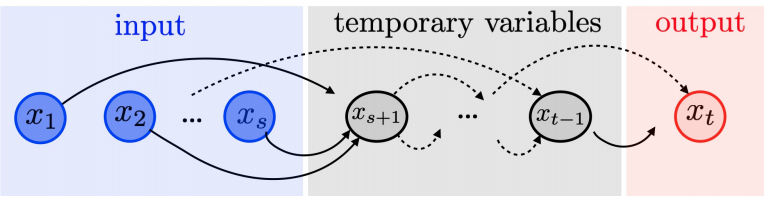
\includegraphics[width=.8\textwidth]{computational_graph.png}
  \\
  \vspace{0.3cm}
  \begin{footnotesize}
    SOURCE:~\citeonline[p.~31]{peyre}.
  \end{footnotesize}
  \label{fig:compgraph}
\end{figure}

The computational graph, \autoref{fig:compgraph}, has the role of
represent the linking of the variables involved in \(f_{k}\) to
\(\bm{x}_{k}\). The evaluation of \(f(\bm{x})\) corresponds to a
forward traversal of this graph. Now, how we evaluate \(f\) through the
graph? Via one of the AD modes.

\subsection{Forward Mode}

The forward mode correspond to the usual way of computing differentials.
The method initialize with the derivative of the input nodes
\[
  \frac{\partial\bm{x}_{1}}{\partial\bm{x}_{1}} =
  \text{Id}_{n_{1} \times n_{1}},\quad
  \frac{\partial\bm{x}_{2}}{\partial\bm{x}_{1}} =
  \mathbf{0}_{n_{2} \times n_{1}},\quad
  \frac{\partial\bm{x}_{s}}{\partial\bm{x}_{1}} =
  \mathbf{0}_{n_{s} \times n_{1}},
\]
and then iteratively make use of the following recursion formula
\begin{align*}
  &\forall~k = s + 1,~\dots,~t,\\
  &\frac{\partial\bm{x}_{k}}{\partial\bm{x}_{1}} =
    \sum_{l~\in~\text{father}(k)}
    \frac{\partial\bm{x}_{k}}{\partial\bm{x}_{l}}\times
    \frac{\partial\bm{x}_{l}}{\partial\bm{x}_{1}} =
    \sum_{l~\in~\text{father}(k)}
    \frac{\partial}{\partial\bm{x}_{l}}
    f_{k}(\bm{x}_{1},~\dots,~\bm{x}_{k-1})\times
    \frac{\partial\bm{x}_{l}}{\partial\bm{x}_{1}}.
\end{align*}
The notation ``father(\(k\))'' denotes the nodes \(l < k\) of the graph
that are connected to \(k\). We make use of \citeonline[p.~32]{peyre}'s
simple example.

\noindent\textbf{Example.}\hspace{.5cm}
Consider the function
\[
  f(x, y) = y\log(x) + \sqrt{y\log(x)}
\]
with the corresponding computational graph being displayed in
\autoref{fig:excompgraph}.

\begin{figure}[H]
  \setlength{\abovecaptionskip}{.0001pt}
  \caption{EXAMPLE OF A SIMPLE COMPUTATIONAL GRAPH}
  \vspace{0.3cm} \centering
  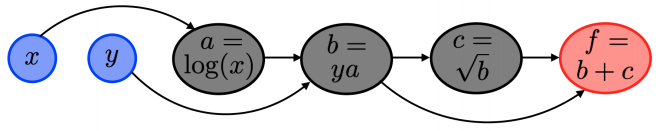
\includegraphics[width=.8\textwidth]{ex-computational_graph.png}
  \\
  \vspace{0.3cm}
  \begin{footnotesize}
    SOURCE:~\citeonline[p.~33]{peyre}.
  \end{footnotesize}
  \label{fig:excompgraph}
\end{figure}

The forward mode iterations to compute the derivative w.r.t. \(x\)
following the computational graph, is given by
\begin{align*}
  \frac{\partial x}{\partial x} &= 1, \quad
  \frac{\partial y}{\partial x} = 0\\
  \frac{\partial a}{\partial x} &=
  \frac{\partial a}{\partial x} \frac{\partial x}{\partial x} =
  \frac{1}{x} \frac{\partial x}{\partial x} \qquad
  &\{x \mapsto a = \log(x)\}\\
  \frac{\partial b}{\partial x} &=
  \frac{\partial b}{\partial a} \frac{\partial a}{\partial x} +
  \frac{\partial b}{\partial y} \frac{\partial y}{\partial x} =
  y \frac{\partial a}{\partial x} + 0 \qquad
  &\{(y, a) \mapsto b = ya\}\\
  \frac{\partial c}{\partial x} &=
  \frac{\partial c}{\partial b} \frac{\partial b}{\partial x} =
  \frac{1}{2\sqrt{b}} \frac{\partial b}{\partial x} \qquad
  &\{b \mapsto c = \sqrt{b}\}\\
  \frac{\partial f}{\partial x} &=
  \frac{\partial f}{\partial b} \frac{\partial b}{\partial x} +
  \frac{\partial f}{\partial c} \frac{\partial c}{\partial x} =
  1 \frac{\partial b}{\partial x} + 1 \frac{\partial c}{\partial x}
  \qquad &\{(b, c) \mapsto f = b + c\}
\end{align*}
To compute the derivative w.r.t. \(y\) we run another forward process
\begin{align*}
  \frac{\partial x}{\partial y} &= 0, \quad
  \frac{\partial y}{\partial y} = 1\\
  \frac{\partial a}{\partial y} &=
  \frac{\partial a}{\partial x} \frac{\partial x}{\partial y} = 0 \qquad
  &\{x \mapsto a = \log(x)\}\\
  \frac{\partial b}{\partial y} &=
  \frac{\partial b}{\partial a} \frac{\partial a}{\partial y} +
  \frac{\partial b}{\partial y} \frac{\partial y}{\partial y} =
  0 + a \frac{\partial y}{\partial y}\qquad
  &\{(y, a) \mapsto b = ya\}\\
  \frac{\partial c}{\partial y} &=
  \frac{\partial c}{\partial b} \frac{\partial b}{\partial y} =
  \frac{1}{2\sqrt{b}} \frac{\partial b}{\partial y} \qquad
  &\{b \mapsto c = \sqrt{b}\}\\
  \frac{\partial f}{\partial y} &=
  \frac{\partial f}{\partial b} \frac{\partial b}{\partial y} +
  \frac{\partial f}{\partial c} \frac{\partial c}{\partial y} =
  1 \frac{\partial b}{\partial y} + 1 \frac{\partial c}{\partial y}
  \qquad &\{(b, c) \mapsto f = b + c\}
\end{align*}

\subsection{Reverse Mode}

Instead of evaluating the differentials for all the input nodes, which
is problematic for a large number of nodes, the reverse mode evaluates
the differentials of the output node w.r.t. all the inner nodes.

The method is based on a backward adjoint chain rule and initialize with
the derivative of the final node
\[
  \frac{\partial\bm{x}_{t}}{\partial\bm{x}_{t}} =
  \text{Id}_{n_{t} \times n_{t}},
\]
and then, from the last to the first node, iteratively make use of the
following recursion formula
\begin{align*}
  &\forall~k = t - 1,~t - 2,~\dots,~1,\\
  &\frac{\partial\bm{x}_{t}}{\partial\bm{x}_{k}} =
    \sum_{m~\in~\text{son}(k)}
    \frac{\partial\bm{x}_{t}}{\partial\bm{x}_{m}}\times
    \frac{\partial\bm{x}_{m}}{\partial\bm{x}_{k}} =
    \sum_{m~\in~\text{son}(k)}
    \frac{\partial\bm{x}_{t}}{\partial\bm{x}_{m}}\times
    \frac{\partial}{\partial\bm{x}_{k}}
    f_{m}(\bm{x}_{1}, \dots, \bm{x}_{m}).
\end{align*}
The notation ``son(\(k\))'' denotes the nodes \(m < k\) of the graph
that are connected to \(k\). To be clear, the same simple example.

\noindent\textbf{Example.}\hspace{.5cm}
Consider, again, the function
\[
  f(x, y) = y\log(x) + \sqrt{y\log(x)}.
\]
The iterations of the reverse mode is given by
\begin{align*}
  \frac{\partial f}{\partial f} &= 1\\
  \frac{\partial f}{\partial c} &=
  \frac{\partial f}{\partial f} \frac{\partial f}{\partial c} =
  \frac{\partial f}{\partial f} 1\qquad &\{c \mapsto f = b + c\}\\
  \frac{\partial f}{\partial b} &=
  \frac{\partial f}{\partial c} \frac{\partial c}{\partial b} +
  \frac{\partial f}{\partial f} \frac{\partial f}{\partial b} =
  \frac{\partial f}{\partial c} \frac{1}{2\sqrt{b}} +
  \frac{\partial f}{\partial f} 1\qquad
  &\{b \mapsto c = \sqrt{b},~b \mapsto f = b + c\}\\
  \frac{\partial f}{\partial a} &=
  \frac{\partial f}{\partial b} \frac{\partial b}{\partial a} =
  \frac{\partial f}{\partial b} y\qquad &\{a \mapsto b = ya\}\\
  \frac{\partial f}{\partial y} &=
  \frac{\partial f}{\partial b} \frac{\partial b}{\partial y} =
  \frac{\partial f}{\partial b} a \qquad &\{y \mapsto b = ya\}
\end{align*}
\begin{align*}
  \frac{\partial f}{\partial x} &=
  \frac{\partial f}{\partial a} \frac{\partial a}{\partial x} =
  \frac{\partial f}{\partial a} \frac{1}{x} \hspace{6.5cm}
  &\{x \mapsto a = \log(x)\}
\end{align*}
This is the advantage of reverse mode over the forward mode. A single
traversal over the computational graph allows to compute both
derivatives w.r.t. \(x\) and \(y\), while the forward mode necessities
two processes.

An drawback of the reverse mode is the need to store the entire
computational graph, which is needed for the reverse sweep. In
principle, storage of this graph is not too difficult to implement.
However, the main benefit of AD is higher accuracy, and in many
applications the cost is not critical.

\section{TMB: TEMPLATE MODEL BUILDER}
\label{cap:tmb}

Note that the goal of AD is not to define an efficient computational
graph, it is up to the user to provide it. However, computing an
efficient graph associated to a mathematical formula is a complicated
combinatorial problem. Thus, since our goal is to be able to fit our
desired statistical models, a computational tool able to efficiently
define and implement this computational graph is make necessary. To
solve this and many other tasks, we have the Template Model Builder
(TMB) developed by \citeonline{TMB}.

TMB \url{ http://tmb-project.org} is an \texttt{R} \cite{R18} package
for fitting statistical latent variable models to data, inpired by AD
Model Builder (ADMB) and developed by \citeonline{ADMB}. ADMB is a
statistical application for fitting nonlinear statistical models and
solve optimization problems, that implements AD using \texttt{C++}
classes and a native template language. Unlike most \texttt{R} packages,
in TMB the model is formulated in \texttt{C++}. This characteristic
provides great flexibility but requires some familiarity with the
\texttt{C}/\texttt{C++} programming language. With TMB a user should be
able to quickly implement complex latent effect models through simple
\texttt{C++} templates.

In this chapter we describe step-by-step all the processes involved in
the creation and parameter estimation of a GLMM. With TMB all this is
put in practice in an efficient and robust fashion.

The user needs to provide just the joint likelihood function writing in
a \texttt{C++} template. When the model presents latent effects, during
the compilation the latent effects will be integrated out via an
efficient Laplace approximation routine with a Newton algorithm inside,
and the marginal log-likelihood gradient will be also computed and
returned. The marginal log-likelihood will be returned into an
\texttt{R} object that can then be optimized using the user's favorite
quasi-Newton routine, available in \texttt{R}. To accomplish all that,
TMB combines some state-of-art software

\begin{itemize}
\item \texttt{CppAD}, a \texttt{C++} AD package
  \url{https://coin-or.github.io/CppAD/};
\item \texttt{Eigen} \cite{eigen}, a \texttt{C++} templated
  matrix-vector library;
\item \texttt{CHOLMOD}, sparse matrix routines available from
  \texttt{R}, used to obtain an efficient implementation of the Laplace
  approximation with exact derivatives
  \url{https://developer.nvidia.com/cholmod};
\item Parallelism through \texttt{BLAS}: Basic Linear Algebra
  Subprograms \url{http://www.netlib.org/blas/}.
\end{itemize}
Also, some of its key characteristics are
\begin{itemize}
\item TMB employs AD to calculate first and second order derivatives of
  the likelihood function or of any objective function written in
  \texttt{C++};
\item The objective function, and its derivatives, can be called from
  \texttt{R}. Hence, parameter estimation via \texttt{optim()} or
  \texttt{nlminb()} is easy to be performed;
\item Standard deviations of any parameter, or derived parameter, can be
  obtained via the \textit{delta method}.
\end{itemize}

Here we focus on GLMMs, but basically any statistical model with a
latent structure (or not), linear (or not), can be fitted with TMB. In
times of \textit{big data} and with the TMB's authors having a
professional preference for state-space and spatial models, TMB has
also automatic sparseness detection.and some other nice built tools. Pre
and post-processing of data should be done in \texttt{R}.

A TMB Users' mailing list exists, and it is extremely helpful for taking
doubts and questions \url{https://groups.google.com/g/tmb-users}. Also,
a very didactic and comprehensive documentation with several examples is
available online
\url{https://kaskr.github.io/adcomp/_book/Tutorial.html}.

% END ==================================================================
% ----------------------------------------------------------------------
\chapter{\(\text{multiGLMM}\): a multinomial GLMM for clustered
  competing risks data}
\label{cap:model}
The clustered competing risks setting is a specific survival data
structure. Although, we are using a general statistical modeling
framework, a generalized linear mixed model (GLMM). Consequently, the
data structure characteristics have to be properly accommodated into the
modeling construction.

To model competing risks data we need a multivariate model and we have
to choose in which scale to work on. We may work on the hazard scale and
deal with the cause-specific hazard function or on the probability scale
and deal with the cause-specific cumulative incidence function (CIF).
By choosing the correct link function, we are able to construct an
appropriate multivariate GLMM to work on the probability scale.

Our goal is to be able to deal with complex family studies, where there
is generally a strong interest in describing age at disease onset in the
scenarios of within-cluster dependence. The distribution of age at
disease onset is directly described by the cause-specific CIF. To build
a multivariate GLMM for this type of data we need to accommodate the
cause-specific CIFs and the censorings. Assuming the conditional
distribution for our model response as multinomial we already deal with
both left-truncation and right-censoring, avoiding the specification of
a censoring distribution.  The cause-specific CIFs can be modeled via
the link function of our, then, multinomial GLMM (multiGLMM). The
multinomial distribution also guarantees that the CIFs of all causes are
modeled.

Our choice for a general framework tries to make the inference of this
complex model, easier. Besides, taking advantage of all the
computational procedures mentioned in the previous chapter. This chapter
presents our multiGLMM for clustered competing risks data and is divided
into two sections. In \autoref{cap:cif} we discuss in detail the
cluster-specific cumulative incidence function (CIF) and in
\autoref{cap:modelitself} we present the complete modeling framework.

\section{CLUSTER-SPECIFIC CUMULATIVE INCIDENCE FUNCTION (CIF)}
\label{cap:cif}

Consider that the observed follow-up time of an individual is given by
\(T = \min(T^{\ast},C)\), where \(T^{\ast}\) denote the failure time
and \(C\) denote the censoring time. Given the possible covariates
\(\bm{x}\), for a cause-specific of failure \(k\), the cumulative
incidence function (CIF) is defined as
\begin{align*}
 F_{k}(t \mid \bm{x})
 = \mathbb{P}[T \leq t,~K = k \mid \bm{x}]
 &= \int_{0}^{t} f_{k}(z \mid \bm{x})~\text{d}z\\
 &= \int_{0}^{t} \lambda_{k}(z \mid \bm{x})~S(z \mid \bm{x})
  ~\text{d}z, \quad t > 0, \quad k = 1,~\dots,~K,
\end{align*}
where \(f_{k}(t \mid \bm{x})\) is the (sub)density for the time to a
type \(k\) failure. This is the general definition of a CIF, and to
define it we need to define the functions that compose the subdensity.
The first is the cause-specific hazard function or process
\[
 \lambda_{k}(t \mid \bm{x}) = \lim_{h \rightarrow 0}~\frac{1}{h}~
 \mathbb{P}[t \leq T < t + h,~K = k \mid T \geq t,~\bm{x}],
 \quad t > 0, \quad k = 1,~\dots,~K.
\]
In words, the cause-specific hazard function \(\lambda_{k}(t \mid
\bm{x})\), represents the instantaneous rate for failures of type
\(k\) at time \(t\) given \(\bm{x}\) and all other failure types
(competing causes). If we sum up all cause-specific hazard functions we
get the overall hazard function,
\[
 \lambda(t \mid \bm{x}) = \sum_{k=1}^{K}\lambda_{k}(t \mid \bm{x}).
\]
From the overall hazard function we arrive in the overall survival
function,
\[
 S(t \mid \bm{x}) = \mathbb{P}[T > t \mid \bm{x}] =
 \exp\left\{-\int_{0}^{t} \lambda(z \mid \bm{x})~\text{d}z\right\},
\]
the second function that compose the subdensity \(f_{k}(t \mid
\bm{x})\). A comprehensive reference for all these definitions is
the book of \citeonline{kalb&prentice}.

Until this point, we were talking about a general CIF's definition. We
need now a precise framework telling us how to take into consideration
our clustered/family structure. We use the same CIF specification of
\citeonline{SCHEIKE} i.e., the approach that motivated this thesis.

For two competing causes of failure, the cause-specific CIFs are
specified in the following manner
\begin{equation}
 F_{k} (t \mid \bm{x},~u_{1},~u_{2},~\eta_{k}) =
 \underbrace{\pi_{k}(\bm{x},~u_{1},~u_{2})}_{
 \substack{\text{cluster-specific}\\\text{risk level}}}\times
  \underbrace{\Phi[w_{k} g(t) - \bm{x}\bm{\gamma}_{k} - \eta_{k}]}_{
   \substack{\text{cluster-specific}\\\text{failure time trajectory}}
  }, \quad t > 0, \quad k = 1,~2,
  \label{eq:cif}
\end{equation}
i.e., as the product of a cluster-specific risk level with a
cluster-specific failure time trajectory, resulting in a
cluster-specific CIF. What makes these components cluster-specific are
\(\bm{u} = \{u_{1},~u_{2}\}\) and \(\bm{\eta} =
\{\eta_{1},~\eta_{2}\}\), Gaussian distributed latent effects with zero
mean and potentially correlated i.e.,
\[
 \begin{bmatrix} u_{1}\\u_{2}\\\eta_{1}\\\eta_{2} \end{bmatrix} \sim
 \parbox{2.5cm}{\centering Multivariate Normal}
 \left(
  \begin{bmatrix} 0\\0\\0\\0\end{bmatrix},
  \begin{bmatrix}
   \sigma_{u_{1}}^{2}&
   \text{cov}(u_{1},~u_{2})&
   \text{cov}(u_{1},~\eta_{1})&\text{cov}(u_{1},~\eta_{2})\\
   &\sigma_{u_{2}}^{2}&
   \text{cov}(u_{2},~\eta_{1})&\text{cov}(u_{2},~\eta_{2})\\
   &&\sigma_{\eta_{1}}^{2}&\text{cov}(\eta_{1},~\eta_{2})\\
   &&&\sigma_{\eta_{2}}^{2}
  \end{bmatrix}
 \right).
\]
The cluster-specific survival function is given by \(S(t \mid
\bm{x},~\bm{u},~\bm{\eta}) = 1 - F_{1} (t \mid
\bm{x},~\bm{u},~\eta_{1}) - F_{2} (t \mid
\bm{x},~\bm{u},~\eta_{2})\). Since we use the same CIF specification
of \citeonline{SCHEIKE}, the following details are essentially the same
encountered in the paper.

Focusing first on the second component of \autoref{eq:cif}, the
cluster-specific failure time trajectory
\[
 \Phi[w_{k} g(t) - \bm{x}\bm{\gamma}_{k} - \eta_{k}],
 \quad t > 0, \quad k = 1,~2,
\]
where \(\Phi(\cdot)\) is the cumulative distribution function of a
standard Gaussian distribution. Instead of \(w_{k} g(t)\), in
\citeonline{SCHEIKE} is specified \(\alpha_{k}(g(t))\) with
\(\alpha_{k}(\cdot)\) being a monotonically increasing function known up
to a finite-dimensional parameter vector, \(w_{k}\). Examples are
monotonically increasing B-splines or piecewise linear functions.
However, to simplify the model structure we consider just the
finite-dimensional parameter vector. The bottom line is that the authors
do the same approach in their applications. With regard to the function
\(g(t)\), it plays a crucial role since the CIF separation in
\autoref{eq:cif} is only possible with it. It is used a time \(t\)
transformation given by
\[
 g(t) = \text{arctanh}\left(\frac{t - \delta/2}{\delta/2}\right),
 \quad t\in(0,~\delta), \quad g(t)\in(-\infty,~\infty),
\]
where \(\delta\) depends on the data and cannot exceed the maximum
observed follow-up time \(\tau\) i.e., \(\delta \leq \tau\). With this
Fisher-based transformation the value of the cluster-specific failure
time trajectory is equal 1, at time \(\delta\). Consequently, \(F_{k}
(\delta \mid \bm{x},~\bm{u},~\eta_{k}) = \pi_{k}(\bm{x} \mid
\bm{u})\) and we can interpret \(\pi_{1}(\bm{x} \mid \bm{u})\) and
\(\pi_{2}(\bm{x} \mid \bm{u})\) as the cause-specific
cluster-specific risk levels, at time \(\delta\).

The cluster-specific risk levels are modeled by a multinomial logistic
regression model with latent effects i.e.,
\begin{equation}
 \pi_{k}(\bm{x}, \bm{u}) =
 \frac{\exp\{\bm{x}\bm{\beta}_{k} + u_{k}\}}{1 +
  \exp\{\bm{x}\bm{\beta}_{1} + u_{1}\} +
  \exp\{\bm{x}\bm{\beta}_{2} + u_{2}\}}, \quad k = 1,~2,
 \label{eq:risklevel}
\end{equation}
where the \(\bm{\beta}_{k}\)'s are the coefficients responsible for
quantifying the impact of the covariates in the cause-specific risk
levels. For individuals from the same chuster/family, at the same time
point, the \(\bm{\beta}_{k}\)s have the well-known odds ratio
interpretation.

A direct understanding of all coefficients/parameters of
\autoref{eq:cif} can be reached via the illustrations in
\autoref{fig:cifcoefs}. To really understand what is going on, we
simplify the model. We still consider just two competing causes but
without covariates and we plot just the cluster-specific CIF of one
failure cause. In \autoref{fig:cifcoefs}~A) we see that the \(\beta\)'s
are also related with the curve's maximum value i.e., bigger the
\(\beta\), highest the CIF will be.

The \(\bm{\gamma}_{k}\)'s are the coefficients responsible for
quantifying the impact of the covariates in the cause-specific failure
time trajectories i.e., the shape of the cumulative incidence. In
\autoref{fig:cifcoefs}~B) we see that the \(\gamma\)'s are also related
with an idea of midpoint and consequently, growth speed. The fact that
\(\gamma_{k}\) enters negatively in the cluster-specific failure time
trajectory makes that a negative value causes an advance towards the
curve, whereas a positive value causes a delay. Last but not least, the
\(w\)'s in \autoref{fig:cifcoefs}~C). With negative values, we have a
decreasing curve and with positive values an increasing curve i.e., we
are interested only on the positive side.

\begin{figure}[H]
 \setlength{\abovecaptionskip}{.0001pt}
 \caption{ILLUSTRATION OF COEFFICIENT BEHAVIORS FOR A GIVEN CUMULATIVE
          INCIDENCE FUNCTION (CIF) (PROPOSED BY \citeonline{SCHEIKE}),
          IN A MODEL WITH TWO COMPETING CAUSES OF FAILURE, WITHOUT
          COVARIATES, AND WITH THE FOLLOWING CONFIGURATION: \(\beta_{2}
          = 0\), \(\bm{u} = 0\) AND \(\bm{\eta} = 0\); IN EACH SCENARIO
          ALL OTHER COEFFICIENTS ARE SET TO ZERO, WITH THE EXCEPTION
          OF \(w_{1} = 1\)}
 \vspace{0.2cm}\centering
 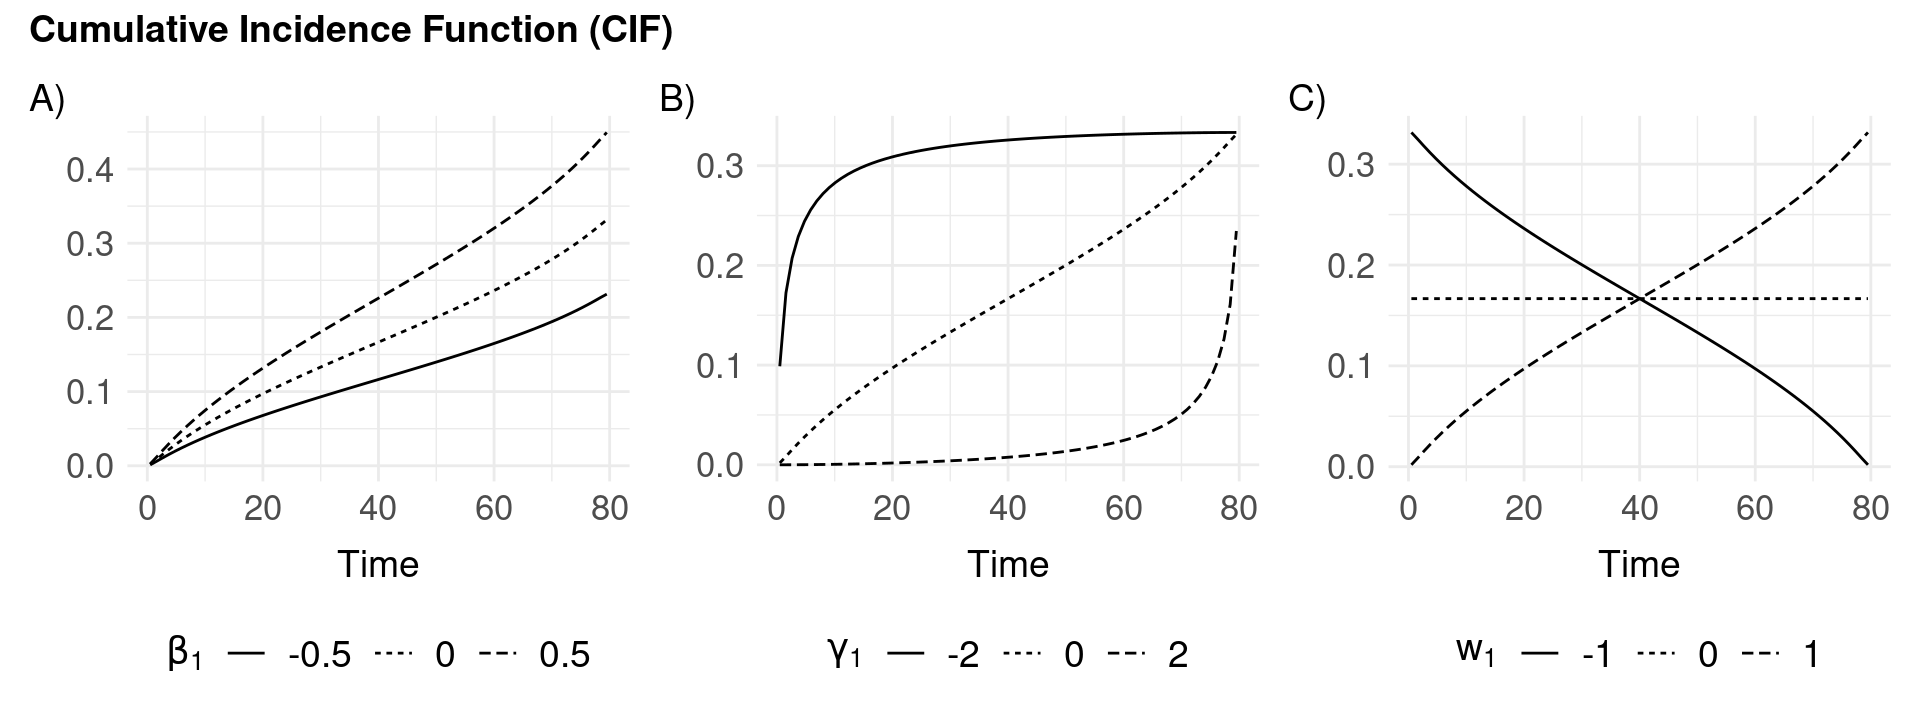
\includegraphics[width=\textwidth]{cifcoefs-1.png}\\
 \begin{footnotesize}
  SOURCE: The author (2021).
 \end{footnotesize}
 \label{fig:cifcoefs}
\end{figure}

Remains to talk about the within-cluster dependence induced by the
latent effects in \(\bm{u}\) and \(\bm{\eta}\). Unfortunately, they do
not have an easy interpretation. To help in the discussion,
\autoref{fig:cif} illustrates the cluster-specific CIF for a given
failure cause in a model without covariates, let us call it failure
cause 1 (in total we have two).

The latent effects \(u_{1}\) and \(u_{2}\) always appear together in the
cluster-specific risk level, as consequency they have a joint effect on
the cumulative incidence of both causes. As we can see in
\autoref{fig:cif}, an increase in \(u_{k}\) will increase the risk of
failure from cause \(k\). The interpretation of
\(\text{cov}(\eta_{1},~\eta_{2})\) and \(\text{cov}(u_{1},~u_{2})\) is
straightforward, and those values are in most of the cases positive, as
said in \citeonline{SCHEIKE}. With regard to
\(\text{cov}(u_{k},~\eta_{k})\), negative values are the common
situation. A negative correlation between \(\eta_{k}\) and \(u_{k}\)
imply that when \(\eta_{k}\) decreases, \(u_{k}\) increases and
conversely when \(\eta_{K}\) increases, \(u_{k}\) decreases. In other
words, an increased risk level is reached quickly and a decreased risk
level is reached later, respectively.

Practical situations with a positive within-cause correlation are hard
to find i.e., where an increased risk level is associated with a late
onset and vice versa. However, a positive cross-cause correlation
between \(\eta\) and \(u\) sounds much more realistic i.e., where late
onset of one failure cause is associated with a high absolute risk of
another failure cause.

\begin{figure}[H]
 \setlength{\abovecaptionskip}{.0001pt}
 \caption{ILLUSTRATION OF A GIVEN CLUSTER-SPECIFIC CUMULATIVE INCIDENCE
          FUNCTION (CIF), PROPOSED BY \citeonline{SCHEIKE}, IN A MODEL
          WITH TWO COMPETING CAUSES OF FAILURE, WITHOUT COVARIATES AND
          THE FOLLOWING CONFIGURATION: \(\beta_{1} = -2\),
          \(\beta_{2} = -1\), \(\gamma_{1} = 1\), \(w_{1} = 3\) AND
          \(u_{2} = 0\). THE VARIATION BETWEEN FRAMES IS GIVEN BY THE
          LATENT EFFECTS \(u_{1}\) AND \(\eta_{1}\)}
 \vspace{0.2cm}\centering
 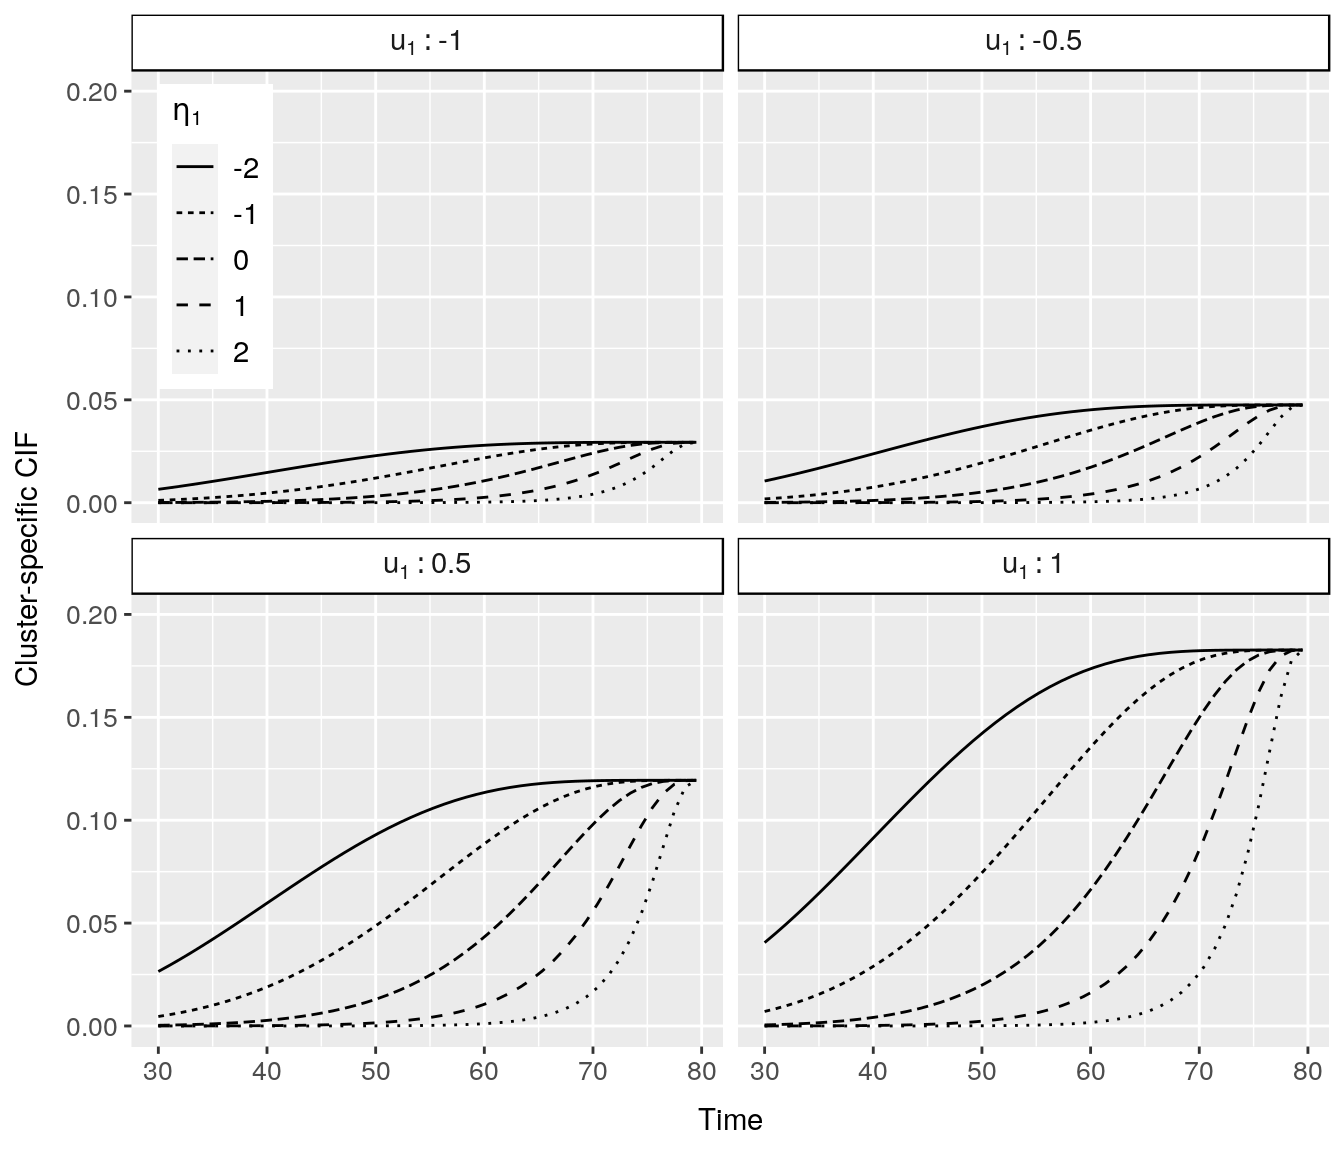
\includegraphics[width=0.9\textwidth]{cif-1.png}\\
 \begin{footnotesize}
  SOURCE: The author (2021).
 \end{footnotesize}
 \label{fig:cif}
\end{figure}

The latent effects \(\{u_{k},~\eta_{k}\}\) are assumed independent
across clusters and shared by individuals within the same
cluster/family.

\section{MODEL SPECIFICATION}
\label{cap:modelitself}

The multiGLMM for clustered competing risks data is specified in the
following hierarchical fashion. By simplicity, we focus on two competing
causes of failure but an extension is straightforward.

For two competing causes of failure, a subject \(i\), in the
cluster/family \(j\), in time \(t\), we have
\begin{align}
 y_{i j t} \mid \{u_{1j},~u_{2j},~\eta_{1j},~\eta_{2j}\}
 &\sim\text{Multinomial}(p_{1ijt},~p_{2ijt},~p_{3ijt})\nonumber\\
 \nonumber\\
 \begin{bmatrix} u_{1}\\u_{2}\\\eta_{1}\\\eta_{2} \end{bmatrix}
 &\sim\text{MN}
  \left(
   \begin{bmatrix} 0\\0\\0\\0 \end{bmatrix},
   \begin{bmatrix}
    \sigma_{u_{1}}^{2}&
    \text{cov}(u_{1},~u_{2})&
    \text{cov}(u_{1},~\eta_{1})&\text{cov}(u_{1},~\eta_{2})\\
    &\sigma_{u_{2}}^{2}&
    \text{cov}(u_{2},~\eta_{1})&\text{cov}(u_{2},~\eta_{2})\\
    &&\sigma_{\eta_{1}}^{2}&\text{cov}(\eta_{1},~\eta_{2})\\
    &&&\sigma_{\eta_{2}}^{2}
   \end{bmatrix}
  \right)\nonumber\\
 \nonumber\\
 p_{kijt}
 &=\frac{\partial}{\partial t}
  F_{k} (t \mid \bm{x},~u_{1},~u_{2},~\eta_{k})\label{eq:model}\\
 &= \frac{\exp\{\bm{x}_{kij}\bm{\beta}_{k} + u_{kj}\}}{
    1 + \sum_{m=1}^{K-1}\exp\{\bm{x}_{mij}\bm{\beta}_{m} + u_{mj}\}}
  \nonumber\\
 &\times w_{k}\frac{\delta}{2\delta t - 2t^{2}}~
  \phi\left(
   w_{k}
   \text{arctanh}\left(\frac{t-\delta/2}{\delta/2}\right)
   - \bm{x}_{kij}\bm{\gamma}_{k} - \eta_{kj}
  \right),\nonumber\\k = 1,~2.\nonumber
\end{align}
The probabilities are given by the derivative w.r.t. time \(t\) of the
cluster-specific CIF. The choice of a multinomial logistic regression
model ensures that the sum of the predicted cause-specific CIFs does not
exceed 1.

Considering two competing causes of failure, we have a multinomial with
three classes. The third class exists to handle the censorship and its
probability is given by the complementary to reach 1. This framework in
\autoref{eq:model} results in what we call multiGLMM, a multinomial
GLMM to handle the CIF of clustered competing risks data. For a random
sample, the corresponding marginal likelihood functions in given by
\begin{align}
 L(\bm{\theta}~;~y)
 &= \prod_{j=1}^{J}~\int_{\Re^{4}}
    \pi(y_{j} \mid \bm{r}_{j})\times\pi(\bm{r}_{j})~\text{d}\bm{r}_{j}
    \nonumber\\
 &= \prod_{j=1}^{J}~\int_{\Re^{4}}
    \Bigg\{
    \underbrace{\prod_{i=1}^{n_{j}}~\prod_{t=1}^{n_{ij}}
    \Bigg(
    \frac{(\sum_{k=1}^{K}y_{kijt})!}{y_{1ijt}!~y_{2ijt}!~y_{3ijt}!}~
    \prod_{k=1}^{K} p_{kijt}^{y_{kijt}}
    \Bigg)}_{\substack{\text{fixed effect component}}}
  \Bigg\}\times\nonumber\\
 &\hspace{2cm}\underbrace{
   (2\pi)^{-2} |\Sigma|^{-1/2} \exp
   \left\{-\frac{1}{2}\bm{r}_{j}^{\top} \Sigma^{-1} \bm{r}_{j}\right\}
   }_{\substack{\text{latent effect component}}}
   \text{d}\bm{r}_{j}\nonumber\\
 &= \prod_{j=1}^{J}~\int_{\Re^{4}}
    \Bigg\{
    \underbrace{\prod_{i=1}^{n_{j}}~\prod_{t=1}^{n_{ij}}
    \prod_{k=1}^{K} p_{kijt}^{y_{kijt}}
    }_{\substack{\text{fixed effect}}}
   \Bigg\}\underbrace{
   (2\pi)^{-2} |\Sigma|^{-1/2} \exp
   \left\{-\frac{1}{2}\bm{r}_{j}^{\top} \Sigma^{-1} \bm{r}_{j}\right\}
   }_{\substack{\text{latent effect component}}}
   \text{d}\bm{r}_{j}\label{eq:loglik},
\end{align}
where \(\bm{\theta} = [\bm{\beta}~\bm{\gamma}~\bm{w}~\bm{\sigma^{2}}~
\bm{\rho}]^{\top}\) is the parameters vector to be maximized. In our
framework, a subject can fail from just one competing cause or get
censor, at a given time. Thus, the fraction of factorials in the fixed
effect component is made only by 0's and 1's. Finally, returning the
value 1. The matrix \(\Sigma\) is the variance-covariance matrix, which
parameters are given by \(\bm{\sigma}^{2}\) and \(\bm{\rho}\).

Now, \autoref{eq:loglik} in words. To each cluster/family \(j\) we have
a product of two components. The fixed effect component, given by a
multinomial distribution with its probabilities specified through the
cluster-specific CIF (\autoref{eq:cif}) and, the latent effect
component, given by a multivariate Gaussian distribution.

To each subject \(i\) that composes a cluster \(j\) we have its specific
fixed effects contribution. The likelihood in \autoref{eq:loglik} is the
most general as possible, allowing for repeated measures to each
subject. Since all subjects of a given cluster shares the same latent
effect, we have just one latent effect contribution multiplying the
product of fixed effect contributions. As we do not observe the latent
effect variables, \(\bm{r}_{j}\), we integrate out in it. With two
competing causes of failure, we have four latent effects (a multivariate
Gaussian distribution in four dimensions). Consequently, for each
cluster, we approximate an integral in four dimensions. The product of
these approximated integrals results in the called marginal likelihood,
to be maximized in \(\bm{\theta}\).

Independent of the parameters value choice, the probabilities for the
failure causes will be small, providing always a bigger probability mass
to the censorship. More will be talked about this model characteristic
in the next chapter.

\subsection{Parametrization}
\label{cap:parametrization}

We have to choose in which terms we parameterize the variance-covariance
matrix \(\Sigma\). Besides the latent effects variances
\(\{\bm{\sigma^{2}}\}\), we have to choose if we will estimate its
covariances or correlations. By the name \textit{variance-covariance}
matrix, it is natural to think on covariance terms. However, this option
is not very attractive since its interpretation is not clear. A more
attractive choice is in terms of correlation.

The covariance between two terms is defined as a triple product: the two
terms standard deviations times the correlation \(\rho\). Still
thinking in two competing causes of failure, we have then an \(\Sigma\)
matrix with six correlations
\begin{align*}
 \Sigma = \begin{bmatrix}
           \sigma_{u_{1}}^{2}&
           \rho_{u_{1},u_{2}}~\sigma_{u_{1}}\sigma_{u_{2}}&
           \rho_{u_{1},\eta_{1}}~\sigma_{u_{1}}\sigma_{\eta_{1}}&
           \rho_{u_{1},\eta_{2}}~\sigma_{u_{1}}\sigma_{\eta_{2}}\\
           &\sigma_{u_{2}}^{2}&
           \rho_{u_{2},\eta_{1}}~\sigma_{u_{2}}\sigma_{\eta_{1}}&
           \rho_{u_{2},\eta_{2}}~\sigma_{u_{2}}\sigma_{\eta_{2}}\\
           &&\sigma_{\eta_{1}}^{2}&
           \rho_{\eta_{1},\eta_{2}}~\sigma_{\eta_{1}}\sigma_{\eta_{2}}\\
           &&&\sigma_{\eta_{2}}^{2}
          \end{bmatrix}.
\end{align*}
With the matrix parametrization being chosen, we have that the
parameters to be estimated are the components of the vector
\(\bm{\theta} = [\bm{\beta}~ \bm{\gamma}~\bm{w}~\bm{\sigma^{2}}~
\bm{\rho}]^{\top}\). There we have the fixed effects or mean components
\(\{\bm{\beta}~\bm{\gamma}~\bm{w}\}\), the easiest to estimate in a
statistical modeling framework; we have variance components
\(\{\bm{\sigma^{2}}\}\), the intermediate ones; and the correlation
components \(\{\bm{\rho}\}\), the hardest ones. This idea of easy or
hard to estimate may be justified by three, connected, arguments.

The first comes from the fact that we are modeling the mean of a
probability distribution in a hierarchical and structured fashion,
consequently, the easiest parameters to estimate will be the mean
components. We may make the analogy that to estimate the mean parameters
we need data (resources); to estimate the variance parameters we need
more data (more resources), and to estimate the correlation parameters
we need much more data (even more resources). The second argument comes
to also explain the first one via the parametric space constraints.

Generally, the fixed effect components do not present constraints i.e.,
they can vary in all \(\mathbb{R}\). The same can not be said from the
variance components, constrained by definition into the
\(\mathbb{R}_{\ast}^{+}\). Finally, we have the correlation components,
constrained to the interval \([-1,~1]\). These parametric space
constraints drive us again to the first argument since we need more
data/resources/information to be able to estimate coefficients
constrained to some interval. Nevertheless, this may not be enough.
Without providing some extra information in terms of an e.g.,
constrained algorithm, it is very reasonable to expect that during the
optimization procedure some unrealistic areas of the parametric space
could be visited and jeopardize the stability or even the whole
optimization procedure. To overcome these possible difficulties,
parameter reparametrizations are more than welcome.

The variance and correlation parameters are modeled in terms of the
matrix \(\Sigma\). This matrix is symmetric and more important, positive
semi-definite. This last characteristic is also the third argument to
justify why is so difficult to estimate these parameters. Since the
estimates should lead to a positive semi-definite matrix, the employment
of a parametrization is welcome to enforces this condition.

In the subject of choosing the components parametrization for a
positive-definite matrix \(\Sigma\), we have basically two big options
available in the statistical modeling literature. One of them consists
of just transform the scale. By practical reasons, let us think in a
\(2\times 2\) matrix
\begin{align*}
 \Sigma = \begin{bmatrix}
           \exp\{\log\sigma_{1}^{2}\}&
           z^{-1}(z(\rho_{1,2}))
           \sqrt{\exp\{\log\sigma_{1}^{2}\}}
           \sqrt{\exp\{\log\sigma_{1}^{2}\}}\\
           &\exp\{\log\sigma_{2}^{2}\}
          \end{bmatrix}
\end{align*}
i.e., in the main diagonal we may now estimate the log-variances and in
the off-diagonal we may estimate Fisher z-transformed correlations.

The estimation of the log-variances has two big advantages
\begin{itemize}
 \item Since the natural logarithm is a real-valued function, we
       overcome the parametric space constraint problem;

 \item High variances are problematic for many reasons but in the
       context of seeing them as the diagonal components of a restricted
       matrix, being able to control its magnitudes is a crucial task to
       the stability of any optimization routine. With the natural
       logarithm transformation we shrink the parametric space as
       illustrated in \autoref{fig:parametrization}~A), avoiding some
       eventual numerical cumbersome.
\end{itemize}
With the correlation components we proceed with the estimation of its
Fischer z-transformation. This transformation, and its inverse, are
defined as
\[
 z(\rho) = \frac{1}{2}\log\left(\frac{1+\rho}{1-\rho}\right)
         = \text{arctanh}(\rho),\quad
 z^{-1}(\rho) = \frac{\exp\{2\rho\}-1}{\exp\{2\rho\}+1}
             = \text{tanh}(\rho).
\]
The Fisher z-transformation plays the role of stretching the small
correlation parametric space but doing this in a smooth fashion, as
illustrated in \autoref{fig:parametrization}~B).

\begin{figure}[H]
 \setlength{\abovecaptionskip}{.0001pt}
 \caption{ILLUSTRATION OF THE PARAMETRIZATION BEHAVIOR FOR THE VARIANCE
          COMPONENTS, IN A), AND CORRELATION COMPONENTS, IN B)}
 \vspace{0.2cm}\centering
 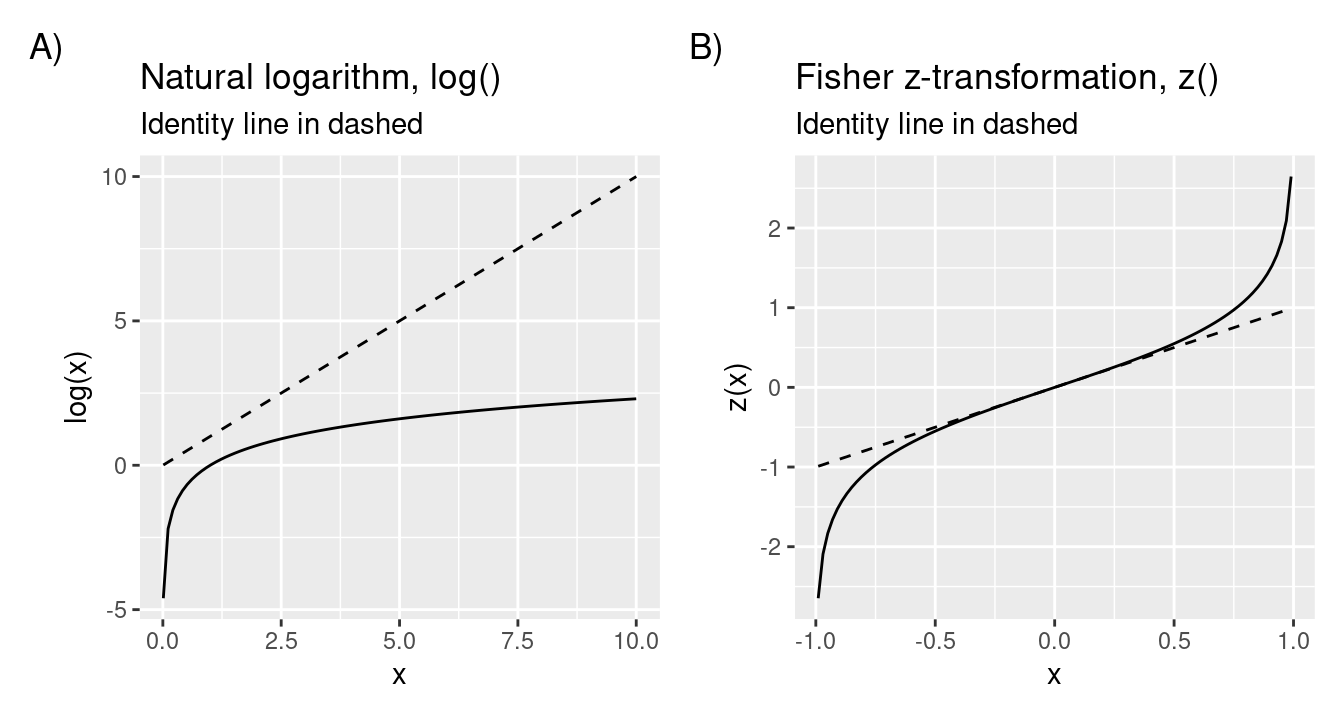
\includegraphics[width=0.8\textwidth]{parametrization-1.png}\\
 \begin{footnotesize}
  SOURCE: The author (2021).
 \end{footnotesize}
 \label{fig:parametrization}
\end{figure}

The other parametrization option consist in estimate the elements of a
factorization or decomposition of the positive-definite matrix
\(\Sigma\). The most common is the Cholesky factorization or
decomposition \cite{cholesky}. For two competing causes of failure, a
standard Cholesky decomposition of \(\Sigma\) may be expressed as
\begin{align*}
 \Sigma = \begin{bmatrix}
           c_{1}&0&0&0\\
           c_{2}&c_{3}&0&0\\
           c_{4}&c_{5}&c_{6}&0\\
           c_{7}&c_{8}&c_{9}&c_{10}
         \end{bmatrix}\begin{bmatrix}
                       c_{1}&c_{2}&c_{4}&c_{7}\\
                       0&c_{3}&c_{5}&c_{8}\\
                       0&0&c_{6}&c_{9}\\
                       0&0&0&c_{10}
                      \end{bmatrix} = LL^{\top},
\end{align*}
where \(\{c_{i}\}_{i=1}^{10}\) are the unconstrained coefficients to be
estimated.

A disadvantage in the use of a decomposition as the Cholesky is the lack
of a straightforward interpretation to the elements
\(\{c_{i}\}_{i=1}^{10}\). However, with the application of the delta
method, already implemented in TMB's \cite{TMB}
\texttt{TMB::sdreport()}, it is straightforward to get back the
\(\Sigma\) elements together with its respective standard errors. The
main advantage of this parametrization apart from the fact that it
ensures positive definiteness, is that it is computationally simple and
stable.

Just to mention another viable possibilities, we could use a modified
Cholesky decomposition \cite{modifiedcholesky} providing a better
statistical interpretation of the decomposition elements or, we could
parametrize the precision matrix, \(\bm{Q} = \Sigma^{-1}\). Since we use
\(\Sigma^{-1}\) in the marginal likelihood of \autoref{eq:loglik},
parametrizing directly its inverse save us some computations.

Besides the popularity of the Cholesky method, there is another
factorization scheme available and efficiently implemented in TMB. It is
a factorization based on a vector scale transformation of an
unstructured correlation matrix. For two competing causes of failure the
decomposition is specified in the following fashion
\[
  \Sigma = VD^{-1/2}LL^{\top}D^{-1/2}V^{\top},
\]
where
\[
 L = \begin{bmatrix}
      1&0&0&0\\
      c_{1}&1&0&0\\
      c_{2}&c_{3}&1&0\\
      c_{4}&c_{5}&c_{6}&1
     \end{bmatrix},\quad D = \text{diag}(LL^{\top})
 \quad\text{ and }\quad W = \text{diag}(\{\sigma_{i}\}_{i=1}^{4}).
\]
This scheme is based initially on the factorization of a correlation
matrix (unit diagonal) as \(D^{-1/2}LL^{\top}D^{-1/2}\). The elements
\(\{c_{i}\}_{i=1}^{6}\) to be estimated has the advantage of being
unconstrained and guarantees that the symmetry and positive definiteness
constraint is respected. The variances are scaled via the diagonal
matrix V, its elements \(\{\sigma_{i}\}_{i=1}^{4}\) are then the
standard deviations to be estimated.

% END ==================================================================

% ----------------------------------------------------------------------
\chapter{simulation study datasets}
\label{cap:datasets}
This chapter describes how to simulate from our multiGLMM and describes
the performed simulation studies. The general simulation procedure is
addressed in \autoref{cap:simu}. In \autoref{cap:data} the simulation
studies are presented in detail.

\section{SIMULATING FROM THE MODEL}
\label{cap:simu}

Being able to simulate data from a model is a key task, fundamental to
assess the finite-sample properties and the estimation procedure
liability of a given statistical model. The step-by-step describing the
simulation procedure of our multiGLMM is presented on Algorithm
\autoref{alg:algo}, following the model hierarchical structure
stipulated in \autoref{eq:model}.

\begin{algorithm}[H]
 \caption{SIMULATING FROM A \(\text{multiGLMM}\) FOR CLUSTERED COMPETING
          RISKS DATA}
 \label{alg:algo}
 \begin{algorithmic}[1]
  \State
   Set \(J\), the number of clusters
  \State
   Set \(n_{j}\), the number of cluster elements
   \Comment{can be of different sizes}
  \State
   Set \(K-1\), the number of competing causes of failure
  \State
   Set the model parameter values \(\bm{\theta} =
   [\bm{\beta}~\bm{\gamma}~\bm{w}~\bm{\sigma^{2}}~\bm{\varrho}]^{\top}\)
  \State
   Sample \(J\) latent effect vectors from a
   \(\mathcal{N}_{(K-1)\times(K-1)}(\bm{0},~\Sigma(\bm{\sigma^{2}},
     \bm{\varrho}))\)
  \State
   Set \(\delta\)
   \Comment{maximum follow-up time}
  \State
   Set the failure times \(t_{ij}\)
  \State
   Compute the competing risks probabilities
   \begin{align*}
    p_{kij} &=
    \frac{\exp\{\bm{x}_{kij}\bm{\beta}_{ki} + u_{kj}\}}{
          1 +
          \sum_{m=1}^{K-1}\exp\{\bm{x}_{mij}\bm{\beta}_{mi} + u_{mj}\}
         }\\
    &\times w_{k}\frac{\delta}{2\delta t_{ij} - 2t_{ij}^{2}}~
     \phi\left(w_{k}
      \text{arctanh}\left(\frac{t_{ij}-\delta/2}{\delta/2}\right) -
      \bm{x}_{kij}\bm{\gamma}_{ki} - \eta_{kj}
     \right),\\
    \text{Censorship}: \quad
    p_{Kij} &=
    1 - \sum_{k=1}^{K-1} p_{kij}, \quad k = 1,~2,~\dots,~K-1
   \end{align*}
  \State
   Sample \(J\times n_{j}\) vectors from a
   \(\text{Multinomial}(p_{1ij},~p_{2ij},~\dots,~p_{Kij})\)
  \State
   If \(t_{ij} = \delta\), moves to class K
   \Comment{any failure at time \(\delta\) is a censorship}
  \State
   \Return
    Multinomial vectors and their respective failure/censoring times
 \end{algorithmic}
\end{algorithm}
\vspace{-1cm}
\begin{footnotesize}
  \begin{center}
    SOURCE: The author (2021).
  \end{center}
\end{footnotesize}

The model described in \autoref{eq:model} is in a general form, allowing
for varying coefficients between clusters. However, we focus on a
simpler structure with just fixed intercepts. Fixing the latent effects
in its distribution mean, zero, and using the following fixed effects
configuration for two competing causes of failure
\begin{align}
 \bm{\beta} &= [-2~~~1.5]^{\top}\nonumber\\
 \bm{\gamma} &= [1.2~~~1]^{\top}\label{eq:fixedconfig}\\
 \bm{w} &= [3~~~5]^{\top}\nonumber,
\end{align}
we get the CIF's and failure probabilities (CIF derivatives w.r.t. time
\(t\), dCIF) presented respectively in \autoref{fig:datasimucif}.

\begin{figure}[H]
 \setlength{\abovecaptionskip}{.0001pt}
 \caption{CUMULATIVE INCIDENCE FUNCTIONS (CIF) AND RESPECTIVE
          DERIVATIVES (\(\text{dCIF}\)) W.R.T. TIME FOR A MODEL WITH
          TWO COMPETING CAUSES OF FAILURE, WITHOUT COVARIATES, LATENT
          EFFECTS AT ZERO, AND FIXED EFFECTS AS IN
          \autoref{eq:fixedconfig}}
 \vspace{0.2cm}\centering
 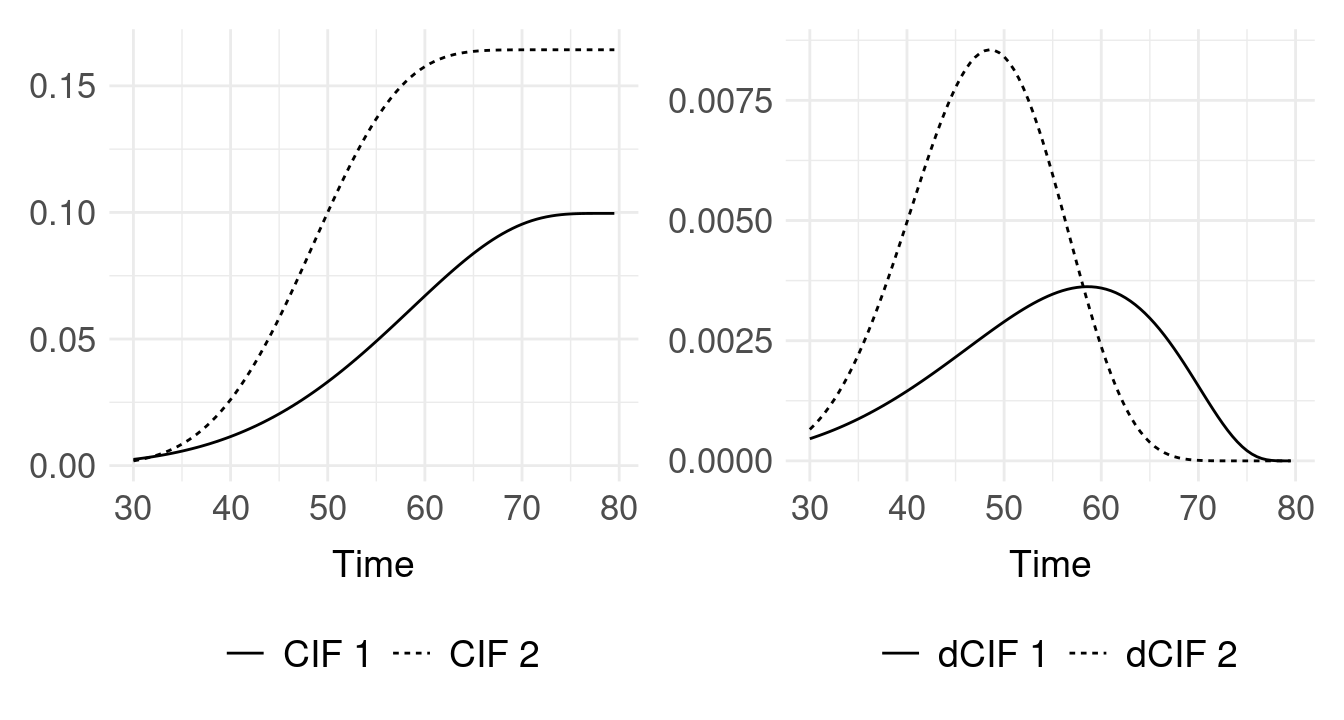
\includegraphics[width=\textwidth]{datasimucif-1.png}\\
 \begin{footnotesize}
  SOURCE: The author (2021).
 \end{footnotesize}
 \label{fig:datasimucif}
\end{figure}

By adding a complete latent structure,
\begin{equation}
 \begin{bmatrix} u_{1}\\u_{2}\\\eta_{1}\\\eta_{2} \end{bmatrix}
 \sim\parbox{2.5cm}{\centering Multivariate Normal}
 \left(\begin{bmatrix} 0\\0\\0\\0 \end{bmatrix},
       \begin{bmatrix}
        1&0.4&0.5&0.4\\
         &1&0.4&0.3\\
         &&1&0.4\\
         &&&1
       \end{bmatrix}
 \right),\label{eq:latentconfig}
\end{equation}
we are able to apply Algorithm \autoref{alg:algo} and generate a
complete model sample with 50000 clusters of size two (pairs),
summarized in \autoref{fig:datasimu}. As already expected from
\autoref{fig:datasimucif}, where the CIF curves maximum are around 15\%,
the simulated failure probabilities and consequently the failure
occurrences, are very small. In this way, we have a data sample filled
with censorship, reflecting the reality of the applications. As disease
incidences, for instance.

\begin{figure}[H]
 \setlength{\abovecaptionskip}{.0001pt}
 \caption{SIMULATED FAILURE CAUSE PROBABILITIES WITH RESPECTIVE OUTPUT
          PCERCENTAGES FOR A MODEL WITH TWO COMPETING CAUSES AND 50000
          CLUSTERS OF SIZE TWO. THE SIMULATION FOLLOWED ALGORITHM
          \autoref{alg:algo} GUIDELINES WITH PARAMETER CONFIGURATIONS
          SPECIFIED IN \autoref{eq:fixedconfig} AND
          \autoref{eq:latentconfig}}
 \vspace{0.2cm}\centering
 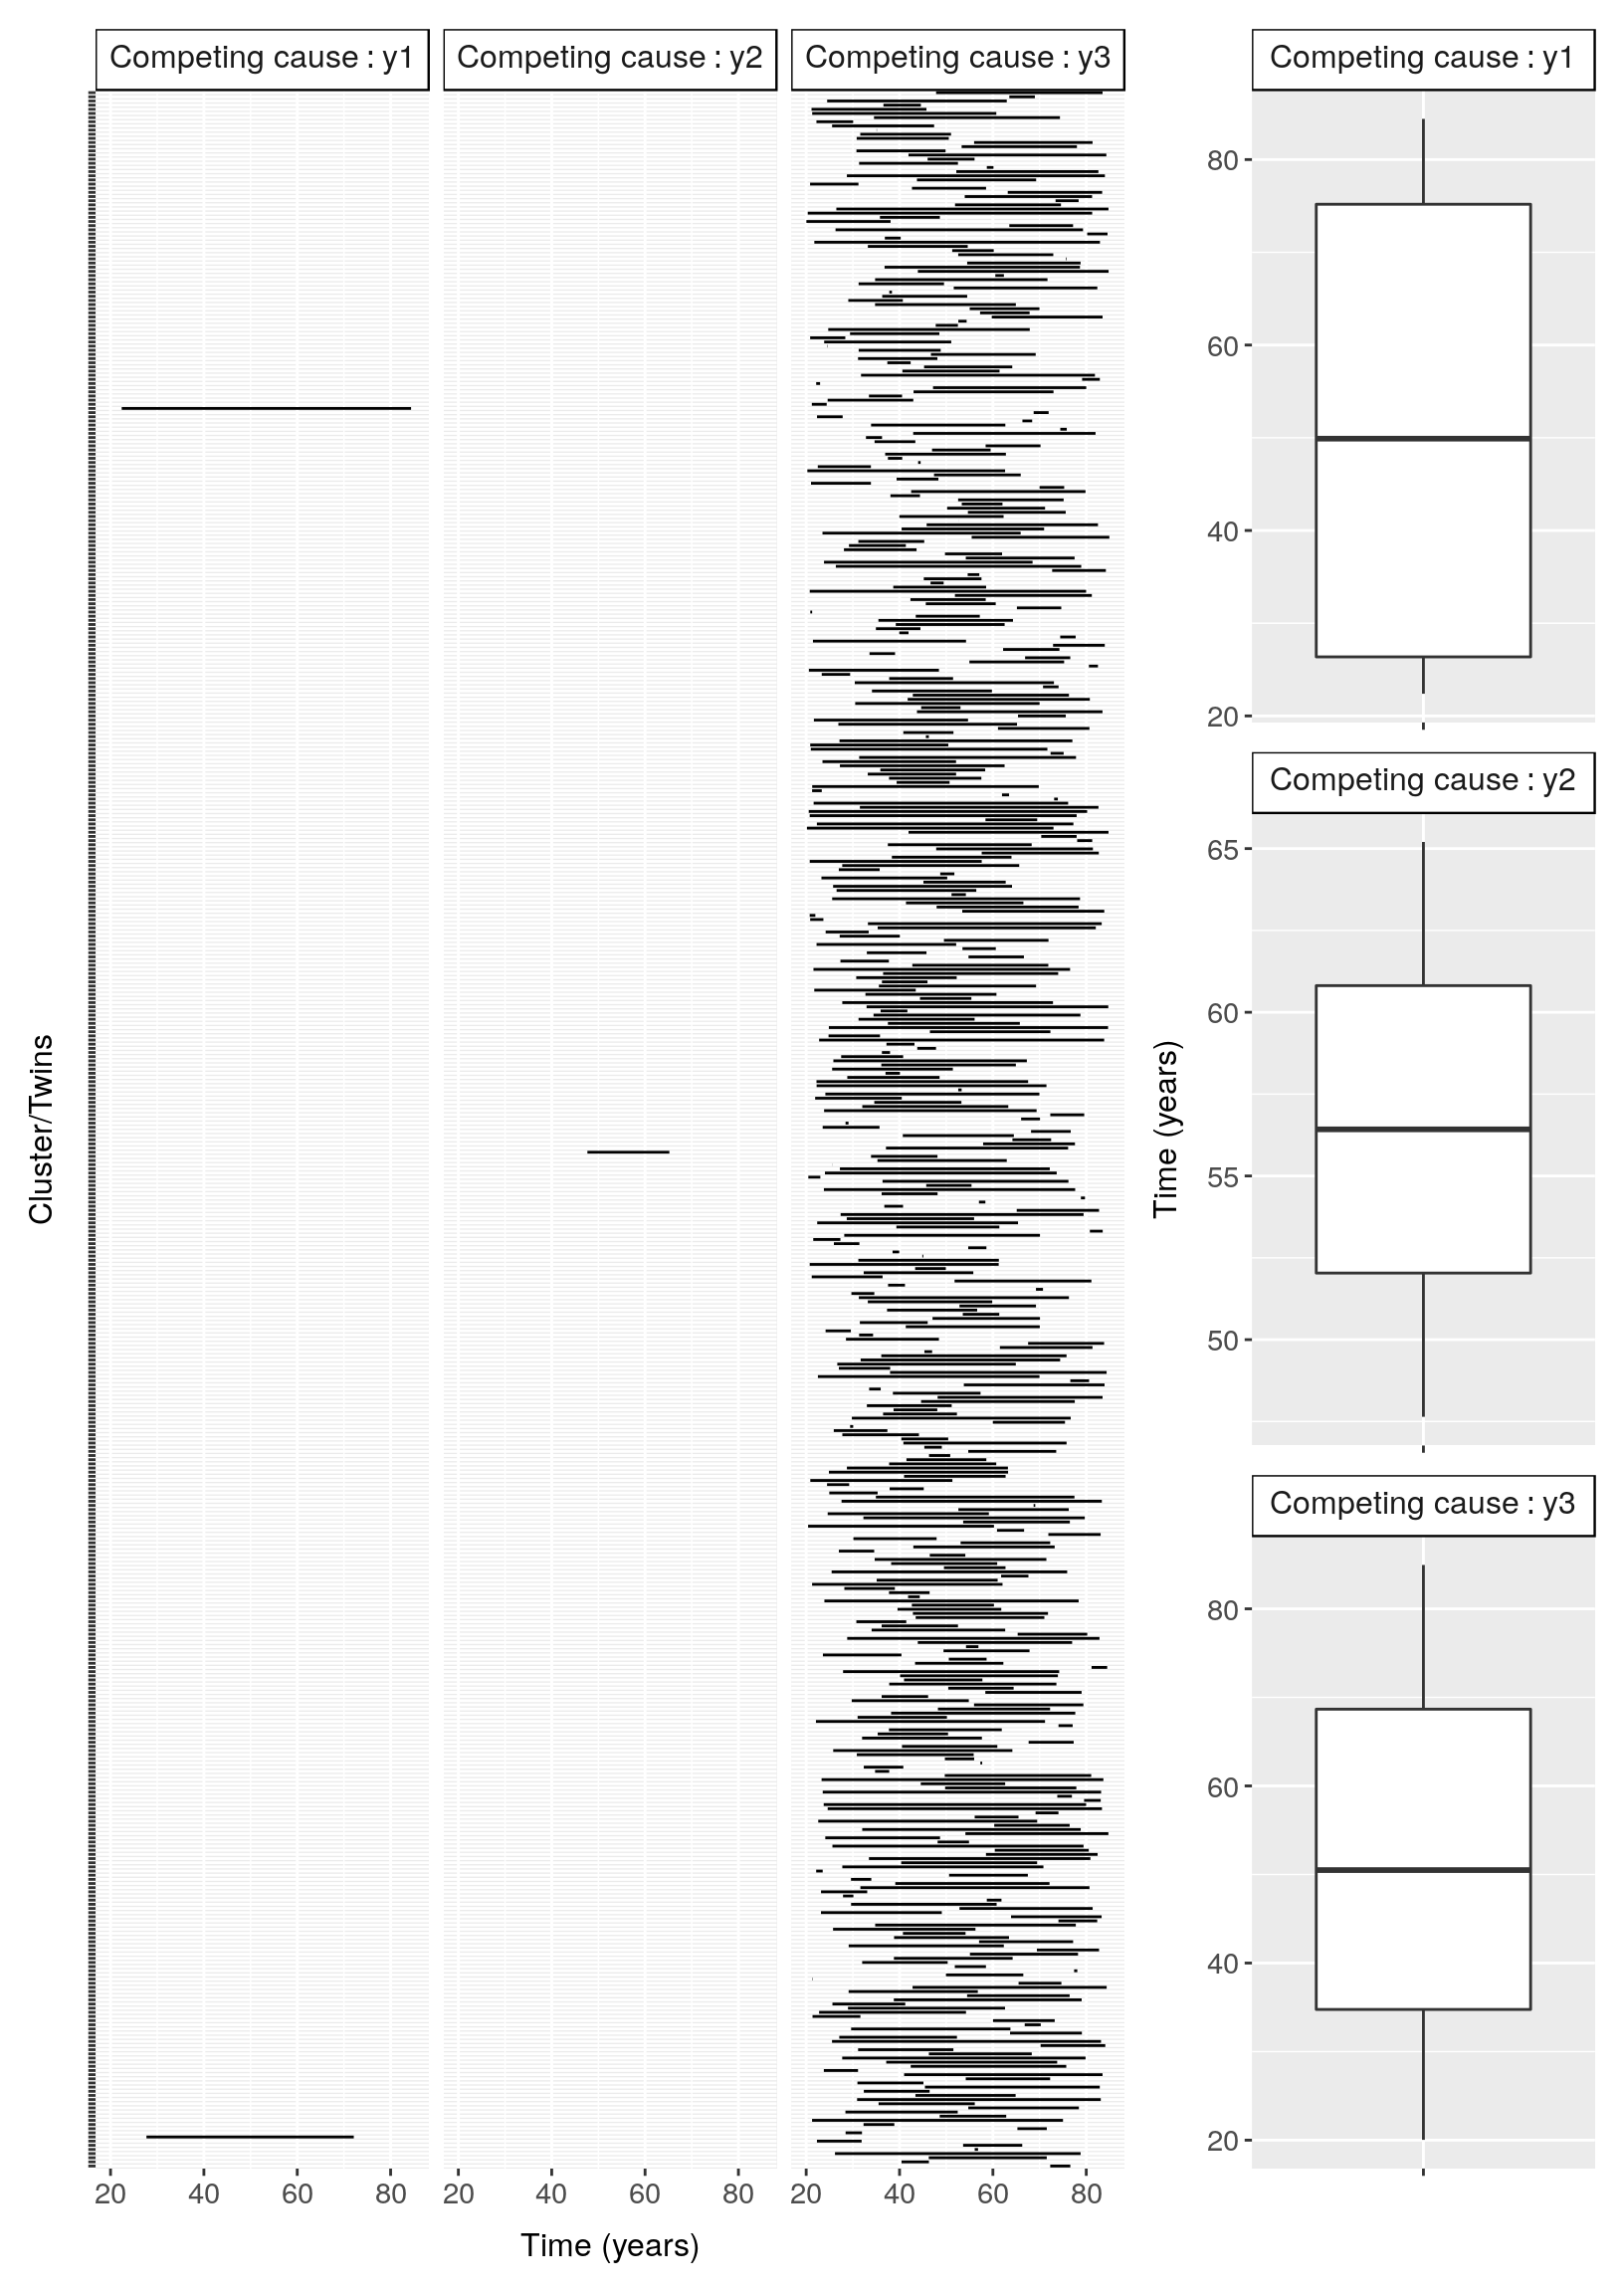
\includegraphics[width=\textwidth]{datasimu-1.png}\\
 \begin{footnotesize}
  SOURCE: The author (2021).
 \end{footnotesize}
 \label{fig:datasimu}
\end{figure}

The \texttt{R} function written to simulate the data is available in
\autoref{cap:appendixC}.

In the simulation routine described in this section,the
failure/censorship times are based on the repetition of an
equally-spaced grid between 30 and 80-time units. A different approach
but still non-parametric would be the random sampling of values between
those limits. Yet, \citeonline{SCHEIKE} does something different through
the sampling of the censorship times from a \(\text{U}(0,~\delta)\), and
the sampling of \(\varsigma\sim\text{U}(0,~1)\) and the computation of
the cause-specific failure times by solving
\[
 \varsigma =
 \Phi\left(w_{k}
           \text{arctanh}\left(\frac{t_{ij}-\delta/2}{\delta/2}\right) -
           \bm{x}_{kij}\bm{\gamma}_{ki} - \eta_{kj}
     \right)
 \quad\text{for}\quad t_{ij},
\]
with \(i\) being the subject, \(j\) the cluster, and \(k\) the failure
cause.

This approach implies a parametric form for the failure times, which we
do not know if holds in the real world.

\section{REAL-BASED DATASET}
\label{cap:data}

% END ==================================================================

% ----------------------------------------------------------------------
\chapter{Results}
\label{cap:results}
This chapter presents the simulation study results.

\section{SIMULATION STUDY}
\label{cap:simures}

We have seventy-two simulation scenarios, detailed in
\autoref{cap:datasets}, and for each one we simulate 300 samples. In
total, we fitted 21600 models. Let us just recap the parameter values
used.
\begin{align*}
 \text{High CIF configuration}:~&\quad
 \{\beta_{1} = -2,~\beta_{2} = -1.5,~\gamma_{1} = 1,~\gamma_{2} = 1.5,~
   w_{1} = 3,~w_{2} = 4
 \};\\
 \text{Low CIF configuration}:~&\quad
 \{\beta_{1} = 3,~\beta_{2} = 2.5,~\gamma_{1} = 2.6,~\gamma_{2} = 4,~
   w_{1} = 5,~w_{2} = 10
 \}.
\end{align*}
\begin{minipage}{0.15\textwidth}
 \begin{align*}
  \sigma_{u_{1}}^{2}   &= 1\\
  \sigma_{u_{2}}^{2}   &= 0.7,\\
  \sigma_{\eta_{1}}^{2} &= 0.6\\
  \sigma_{\eta_{2}}^{2} &= 0.9
 \end{align*}
\end{minipage}%
\begin{minipage}{0.85\textwidth}
 \[
  \text{Correlation structure}~=~\begin{blockarray}{ccccc}
                                  u_{1} & u_{2} & \eta_{1} & \eta_{2}\\
                                  \begin{block}{(cccc)c}
                                   1 & 0.1 & -0.5 &  0.3 & u_{1}\\
                                     &   1 &  0.3 & -0.4 & u_{2}\\
                                     &     &    1 &  0.2 & \eta_{1}\\
                                     &     &      &    1 & \eta_{2}\\
                                  \end{block}
                                 \end{blockarray}.
 \]
\end{minipage}

\vspace{0.3cm}
\noindent
The parameter values per se are not important here. What is important is
to keep in mind the behaviors implied and see if the proposed model is
able to learn the true values in several different scenarios and measure
the quality of this learning.

For the fixed-effect parameters, the take-home message is that we can
build different level CIF scenarios. The \(\bm{\beta}\)s are responsible
for the curve maximum point or plateau, the \(\bm{\gamma}\)s and
\(\bm{w}\)s are responsible for basically the curve shape. Its
interpretation is presented in detail in \autoref{cap:model}.

For the latent structure, the chosen variances and correlations are
considerably high but still acceptable. The underlying idea was to try
to build a realistic variance-covariance scenario and consequently be
able to check how the model performs in such conditions. In the
following pages we have several graphs summarizing the parameters bias,
they are
\begin{align*}
 \bm{\beta}:&\quad\text{\autoref{fig:biassdbeta1}},~
                  \text{\autoref{fig:biassdbeta2}};\hspace{8cm}\\
 \bm{\gamma}:&\quad\text{\autoref{fig:biassdgama1}}~,
                   \text{\autoref{fig:biassdgama2}};\\
 \bm{w}:&\quad\text{\autoref{fig:biassdw1}},~
              \text{\autoref{fig:biassdw2}};\\
 \bm{\sigma^{2}}:&\quad\text{\autoref{fig:biassdlogs2_1}},~
                      \text{\autoref{fig:biassdlogs2_2}},~
                      \text{\autoref{fig:biassdlogs2_3}},~
                      \text{\autoref{fig:biassdlogs2_4}};\\
 \bm{\rho}:&\quad\text{\autoref{fig:biassdrhoz12}},~
                 \text{\autoref{fig:biassdrhoz34}},~
                 \text{\autoref{fig:biassdrhoz4}}.
\end{align*}

\begin{figure}[H]
 \setlength{\abovecaptionskip}{.0001pt}
 \caption{PARAMETER \(\beta_{1}\) BIAS WITH \(\pm\) 1.96 STANDARD
          DEVIATIONS}
 \vspace{0.2cm}\centering
 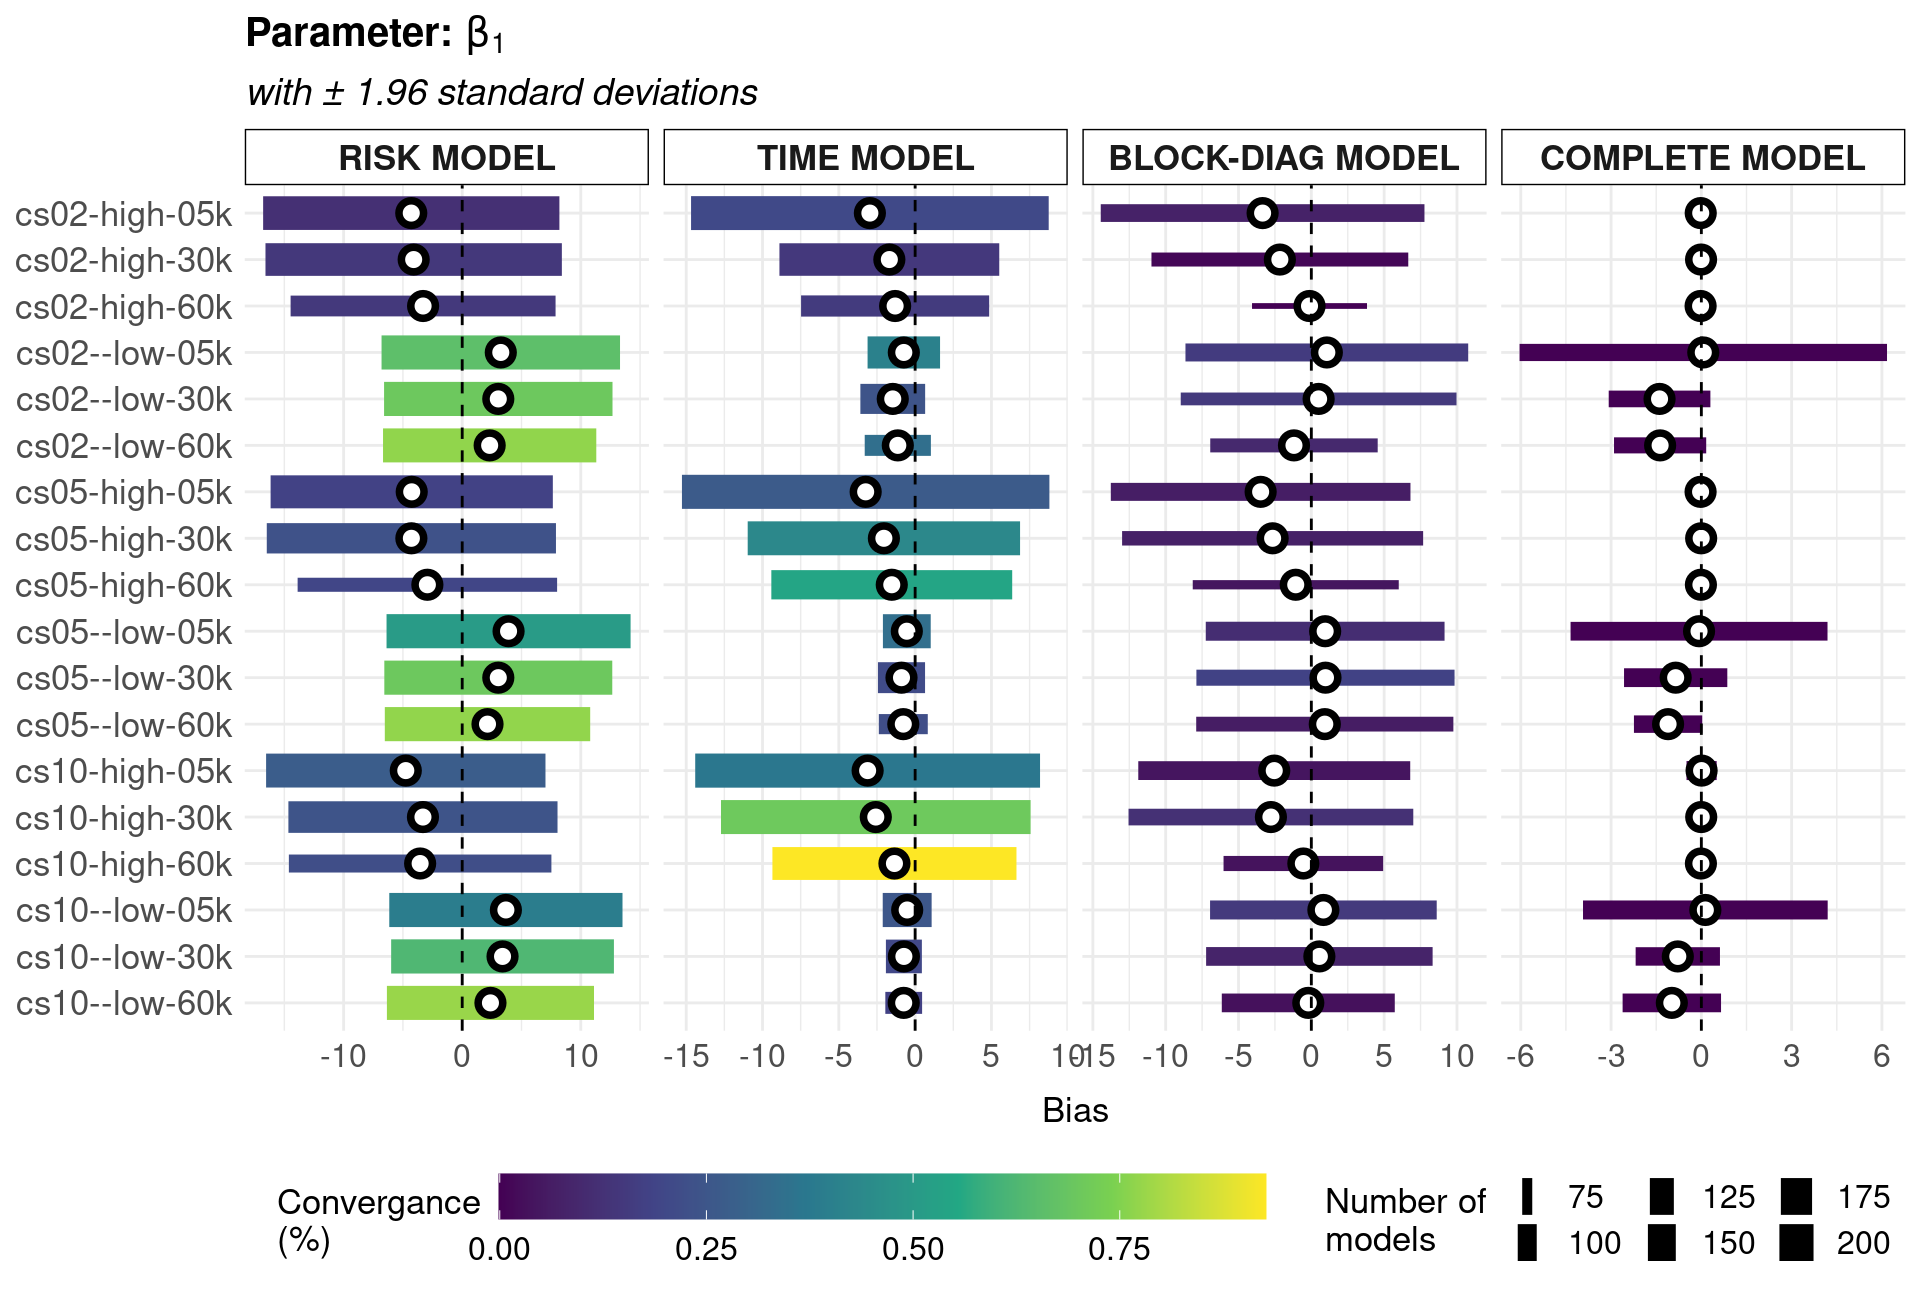
\includegraphics[width=\textwidth]{bias2plotsd-1.png}\\
 \begin{footnotesize}
  SOURCE: The author (2021).
 \end{footnotesize}
 \label{fig:biassdbeta1}
\end{figure}

\begin{figure}[H]
 \setlength{\abovecaptionskip}{.0001pt}
 \caption{PARAMETER \(\beta_{2}\) BIAS WITH \(\pm\) 1.96 STANDARD
         DEVIATIONS}
 \vspace{0.2cm}\centering
 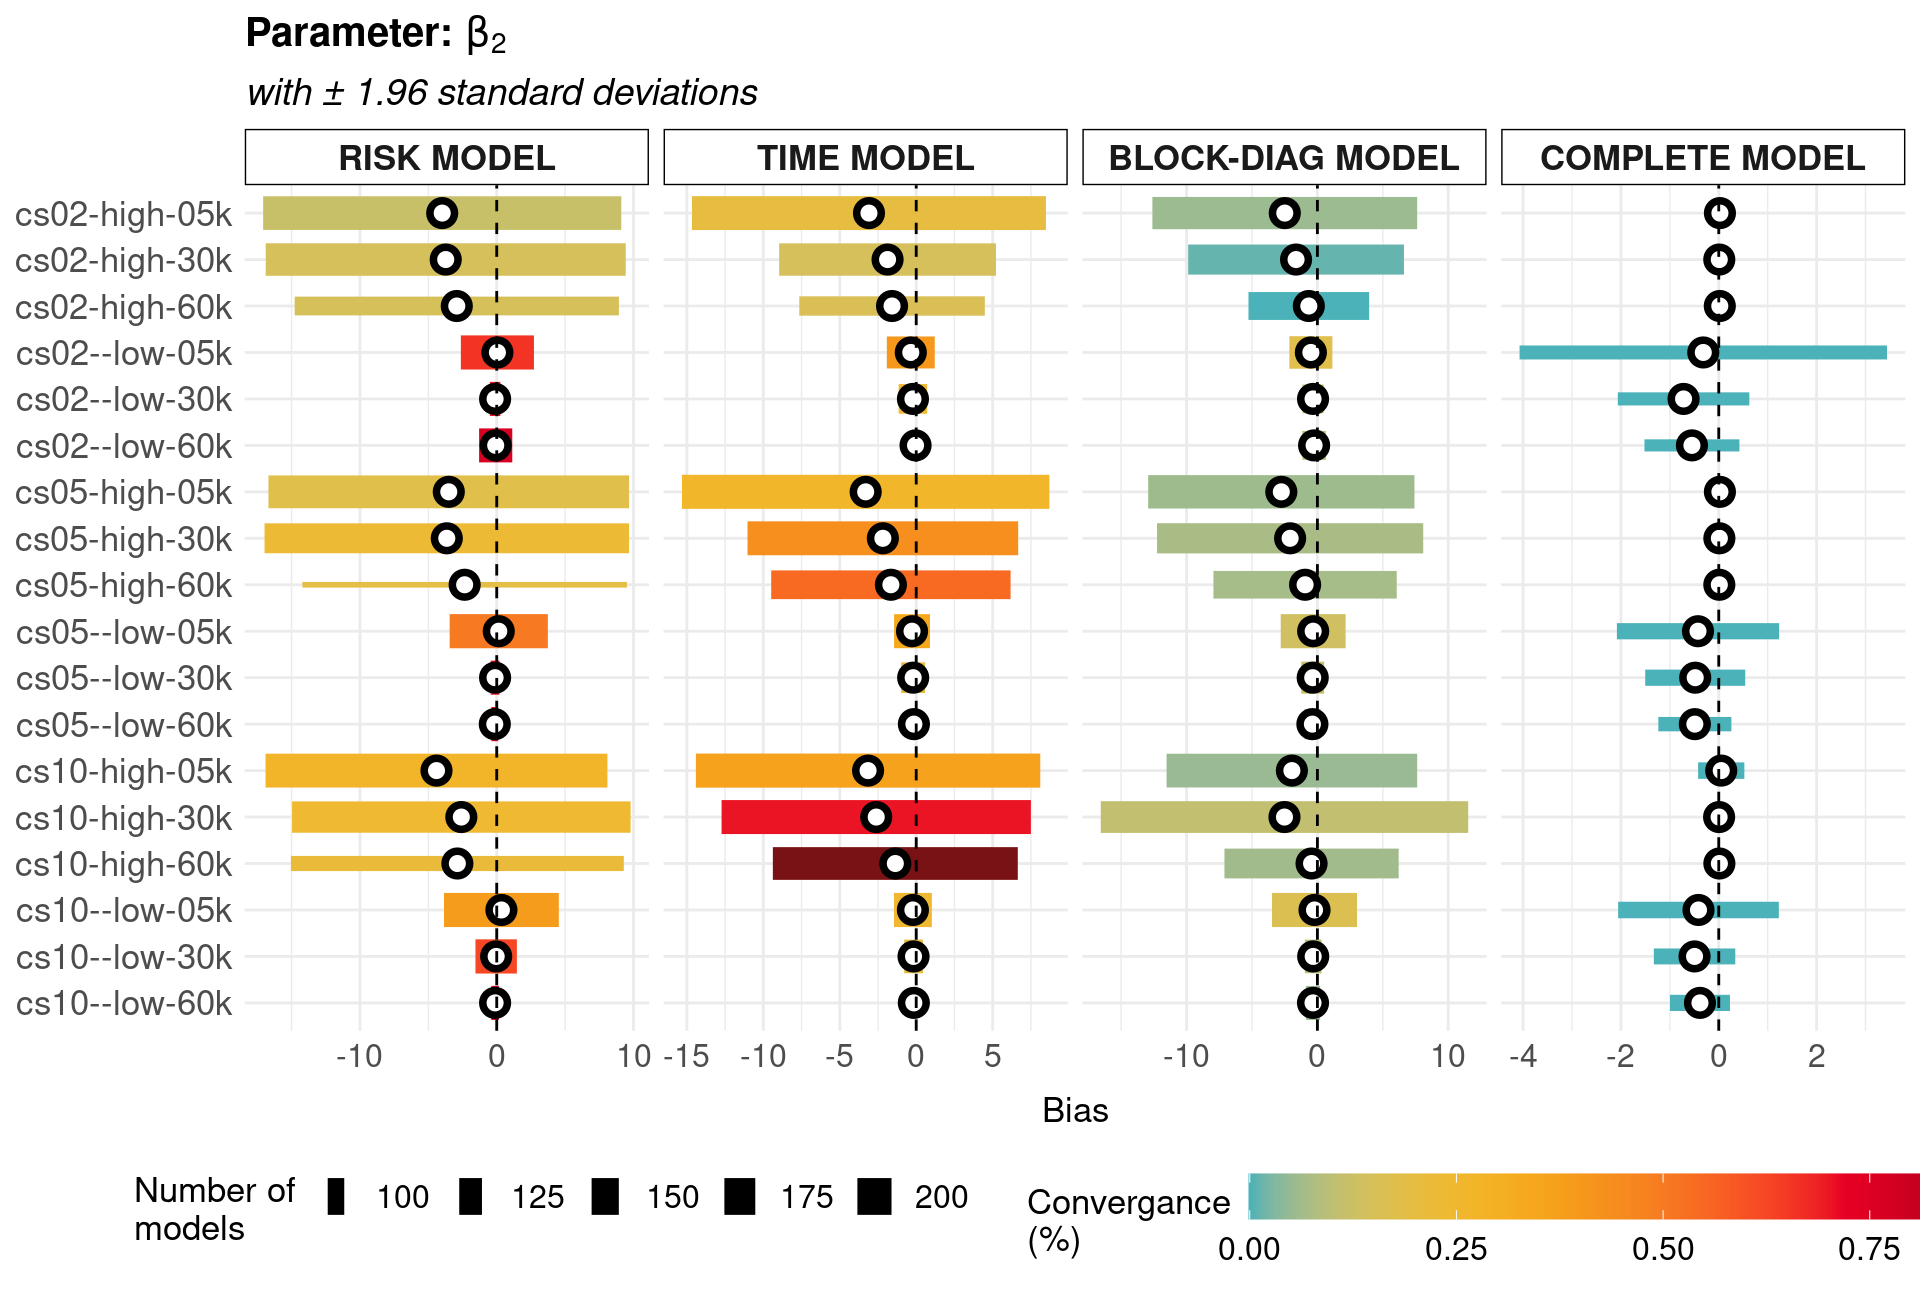
\includegraphics[width=\textwidth]{bias2plotsd-2.png}\\
 \begin{footnotesize}
  SOURCE: The author (2021).
 \end{footnotesize}
 \label{fig:biassdbeta2}
\end{figure}

\begin{figure}[H]
 \setlength{\abovecaptionskip}{.0001pt}
 \caption{PARAMETER \(\gamma_{1}\) BIAS WITH \(\pm\) 1.96 STANDARD
          DEVIATIONS}
 \vspace{0.2cm}\centering
 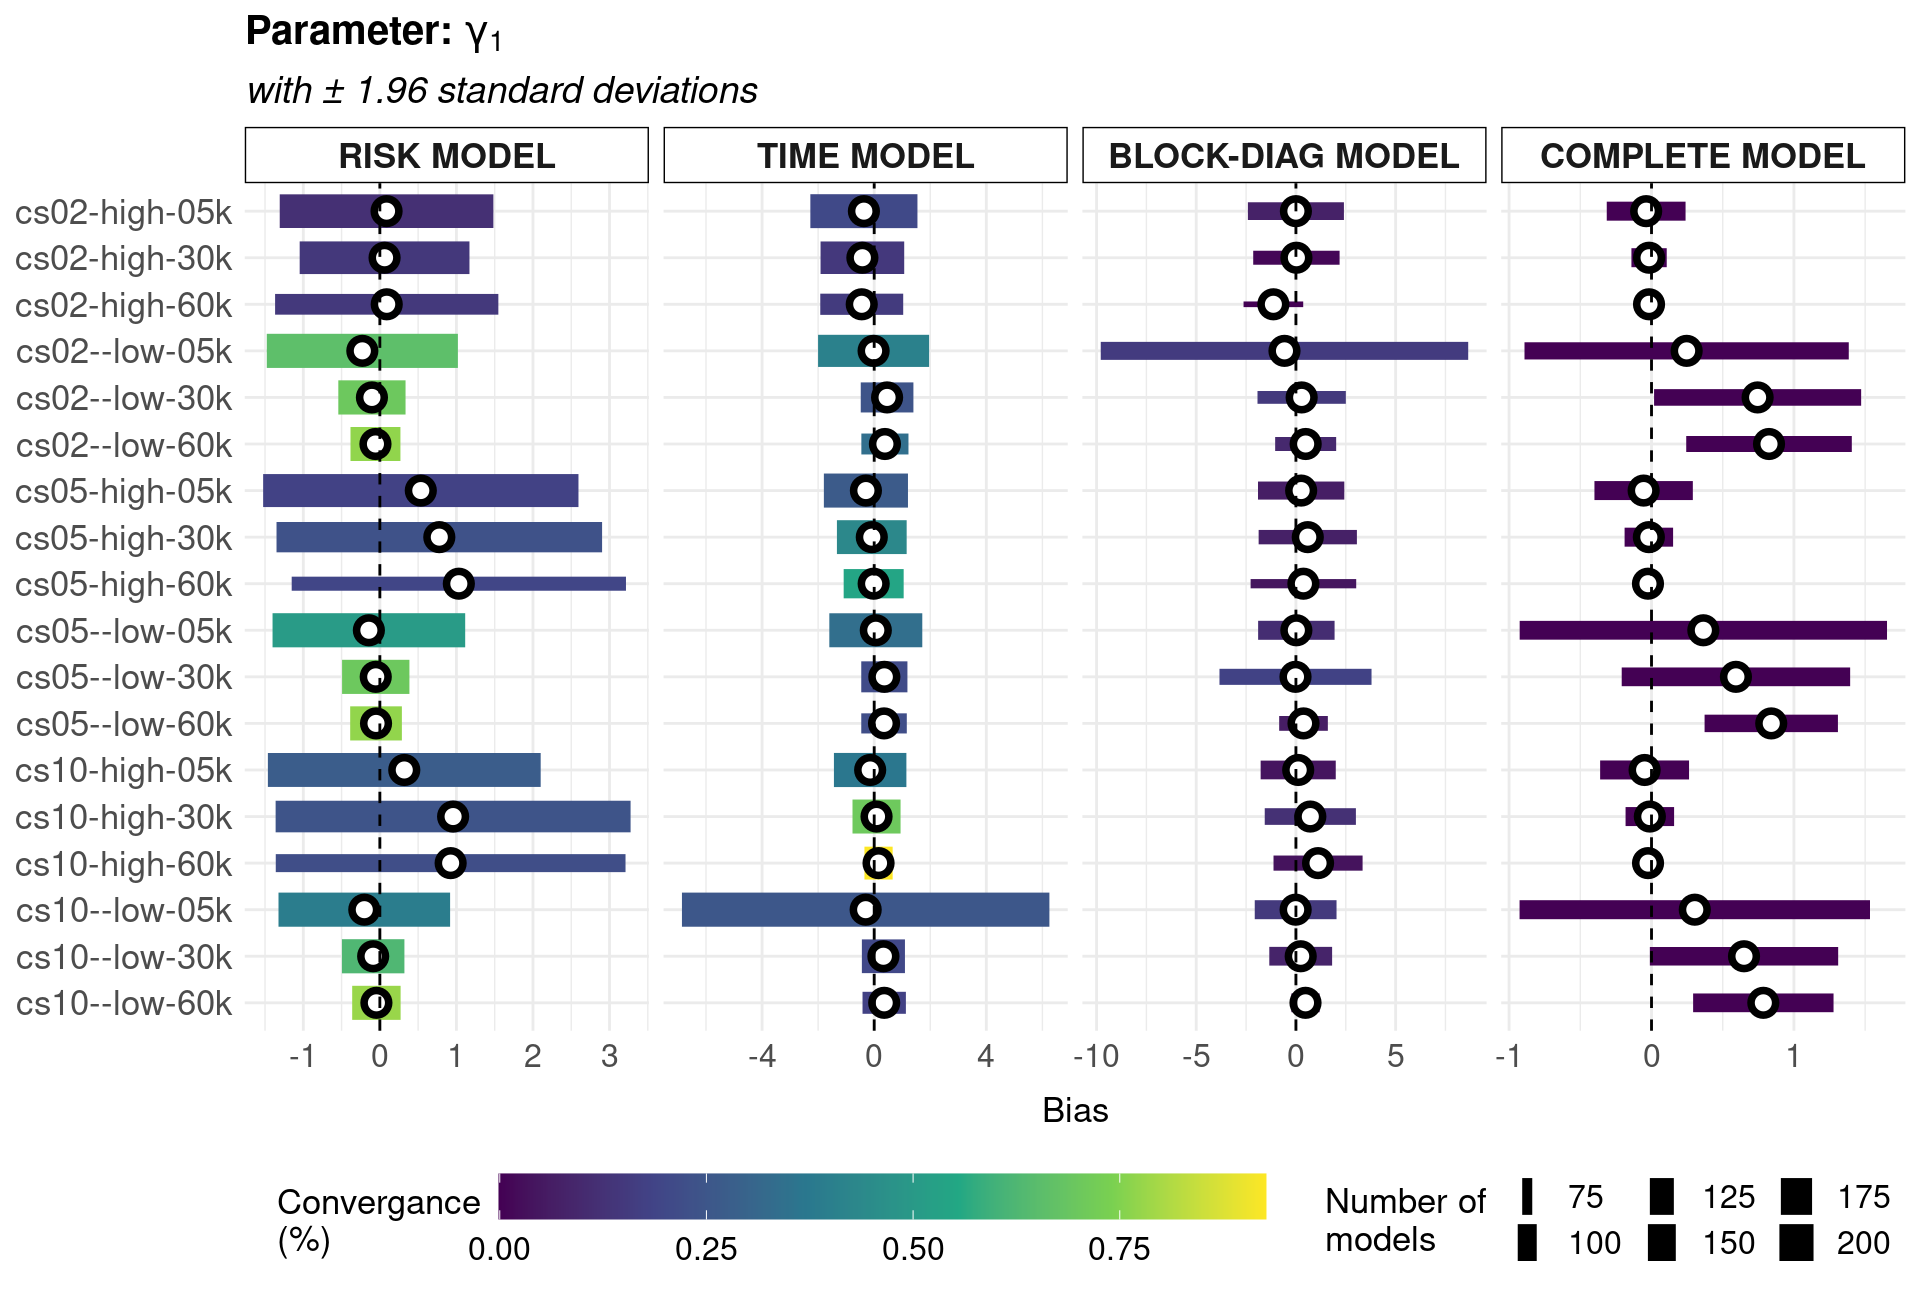
\includegraphics[width=\textwidth]{bias2plotsd-3.png}\\
 \begin{footnotesize}
  SOURCE: The author (2021).
 \end{footnotesize}
 \label{fig:biassdgama1}
\end{figure}

\begin{figure}[H]
 \setlength{\abovecaptionskip}{.0001pt}
 \caption{PARAMETER \(\gamma_{2}\) BIAS WITH \(\pm\) 1.96 STANDARD
          DEVIATIONS}
 \vspace{0.2cm}\centering
 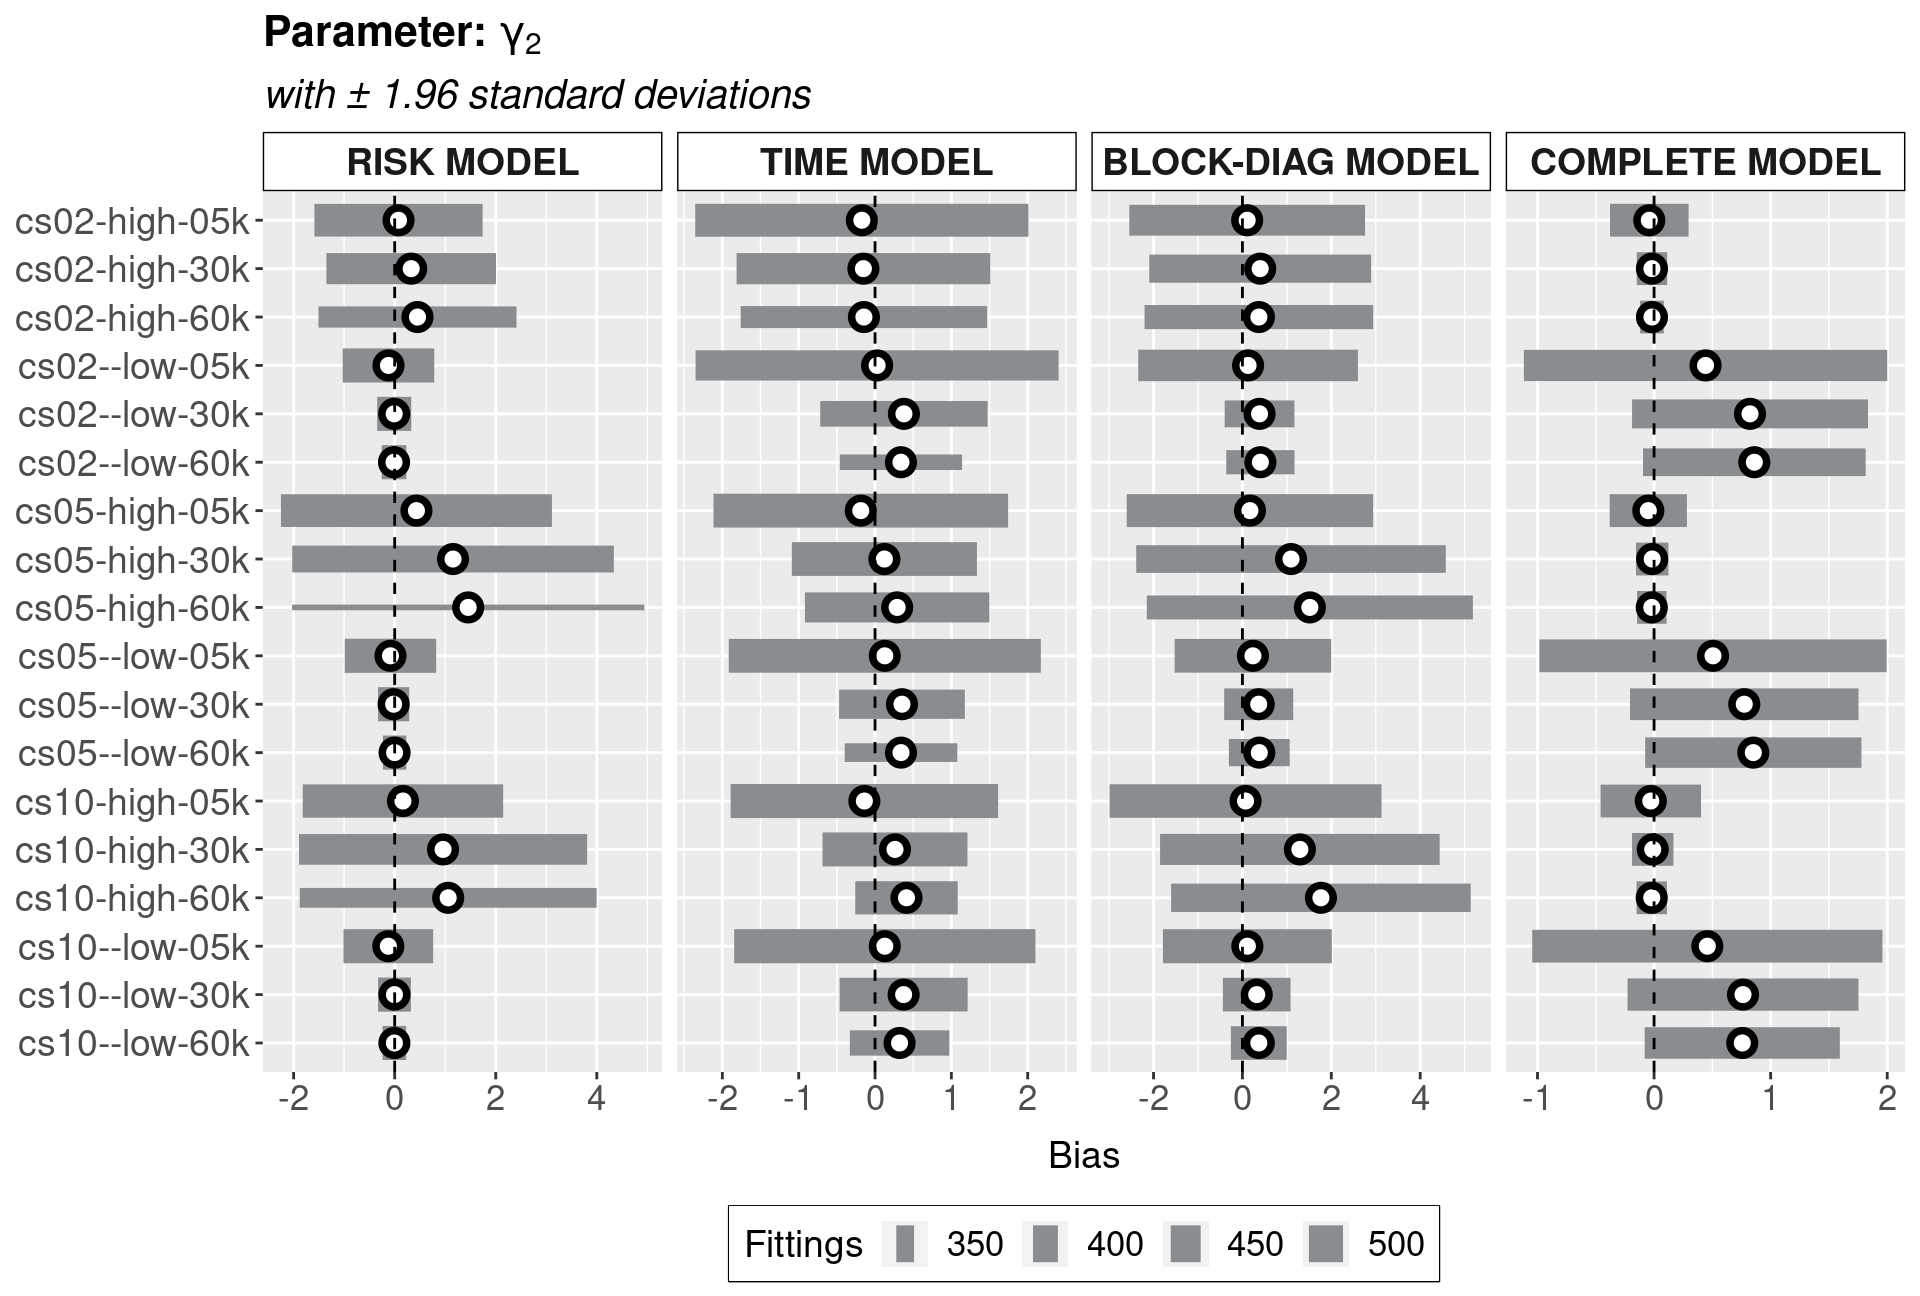
\includegraphics[width=\textwidth]{bias2plotsd-4.png}\\
 \begin{footnotesize}
  SOURCE: The author (2021).
 \end{footnotesize}
 \label{fig:biassdgama2}
\end{figure}

\begin{figure}[H]
 \setlength{\abovecaptionskip}{.0001pt}
 \caption{PARAMETER \(w_{1}\) BIAS WITH \(\pm\) 1.96 STANDARD DEVIATIONS}
 \vspace{0.2cm}\centering
 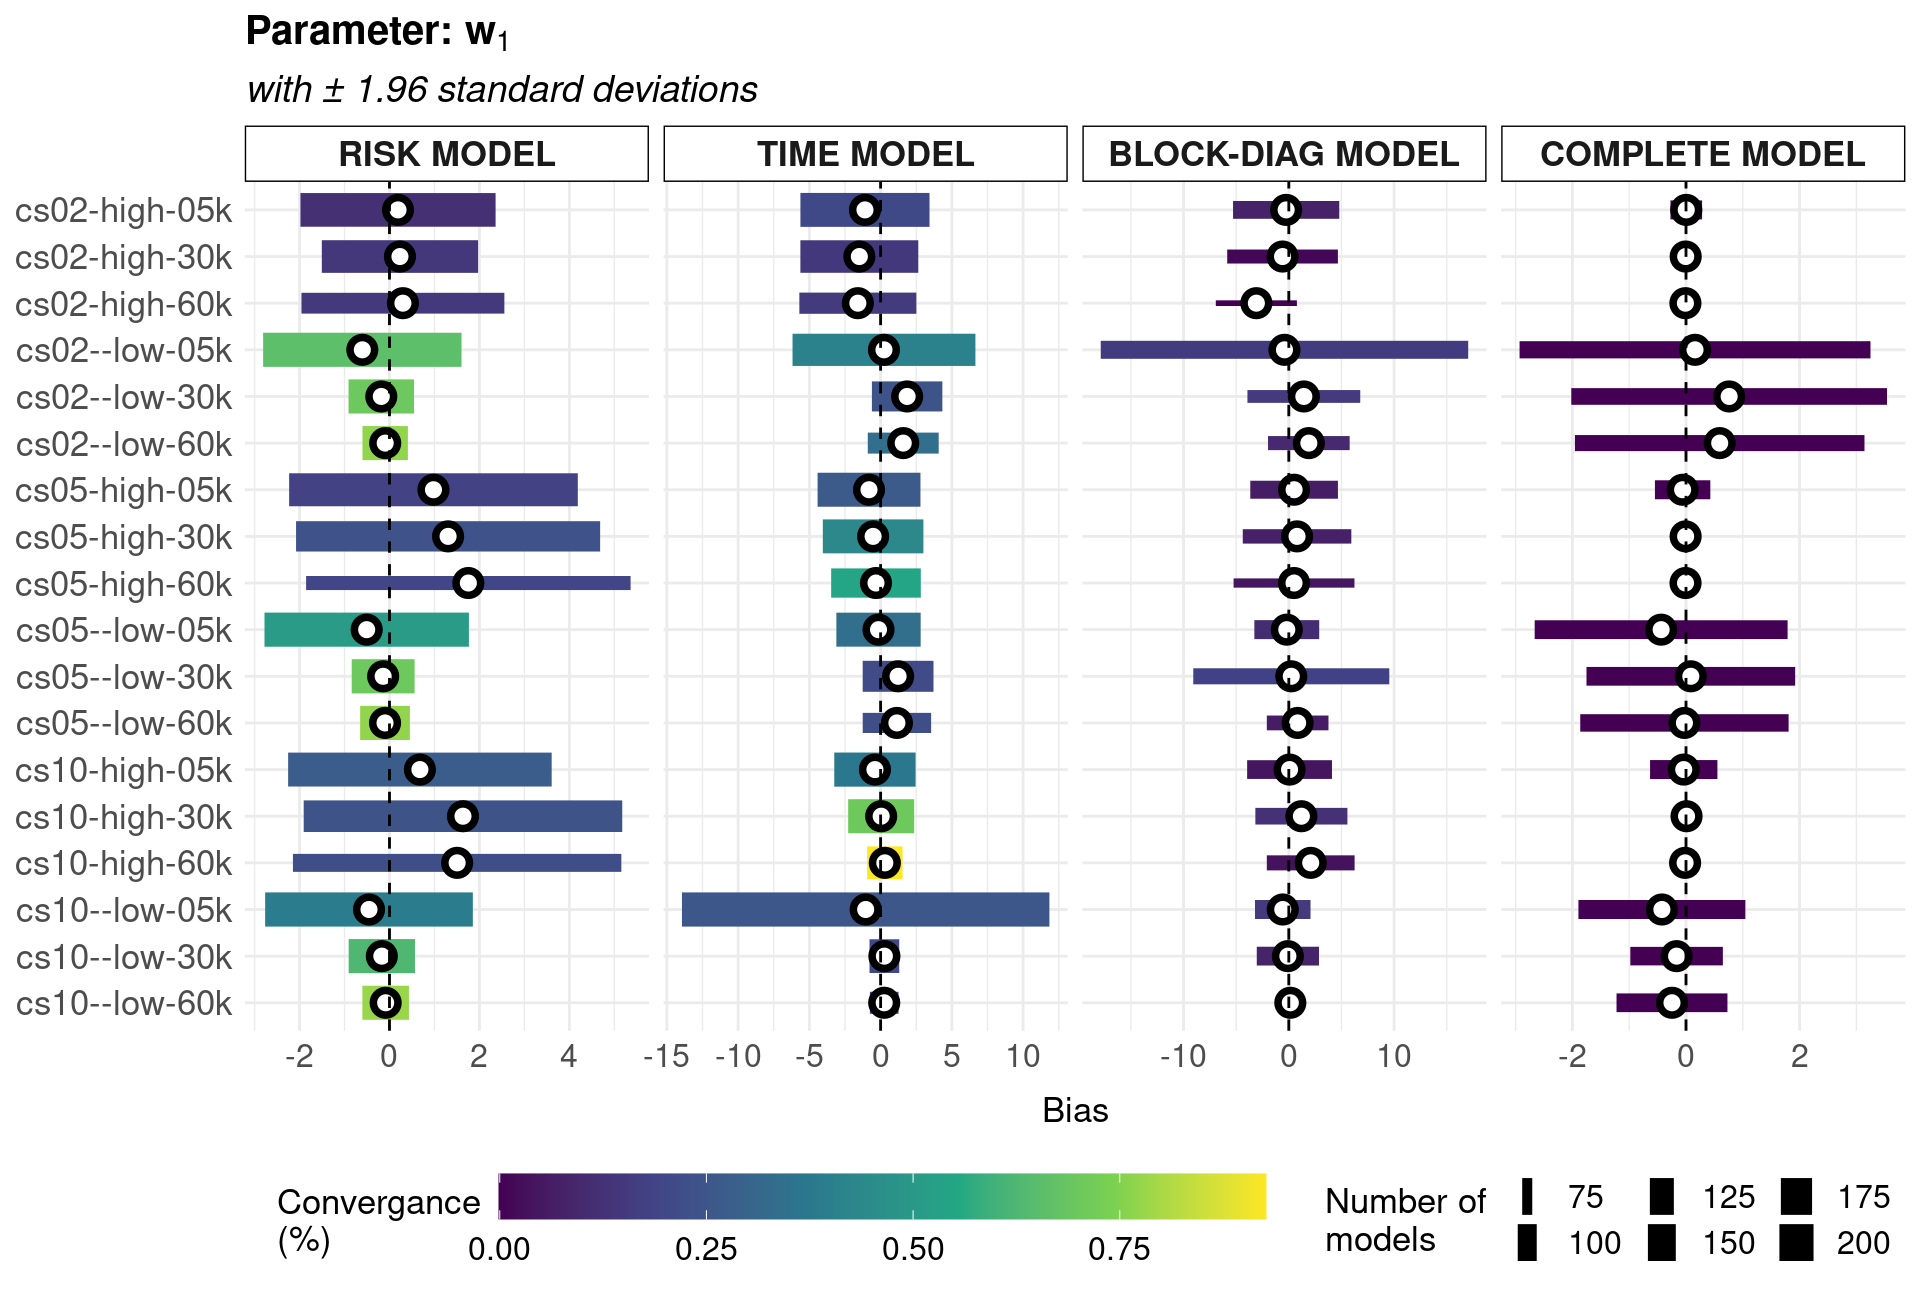
\includegraphics[width=\textwidth]{bias2plotsd-5.png}\\
 \begin{footnotesize}
  SOURCE: The author (2021).
 \end{footnotesize}
 \label{fig:biassdw1}
\end{figure}

\begin{figure}[H]
 \setlength{\abovecaptionskip}{.0001pt}
 \caption{PARAMETER \(w_{2}\) BIAS WITH \(\pm\) 1.96 STANDARD DEVIATIONS}
 \vspace{0.2cm}\centering
 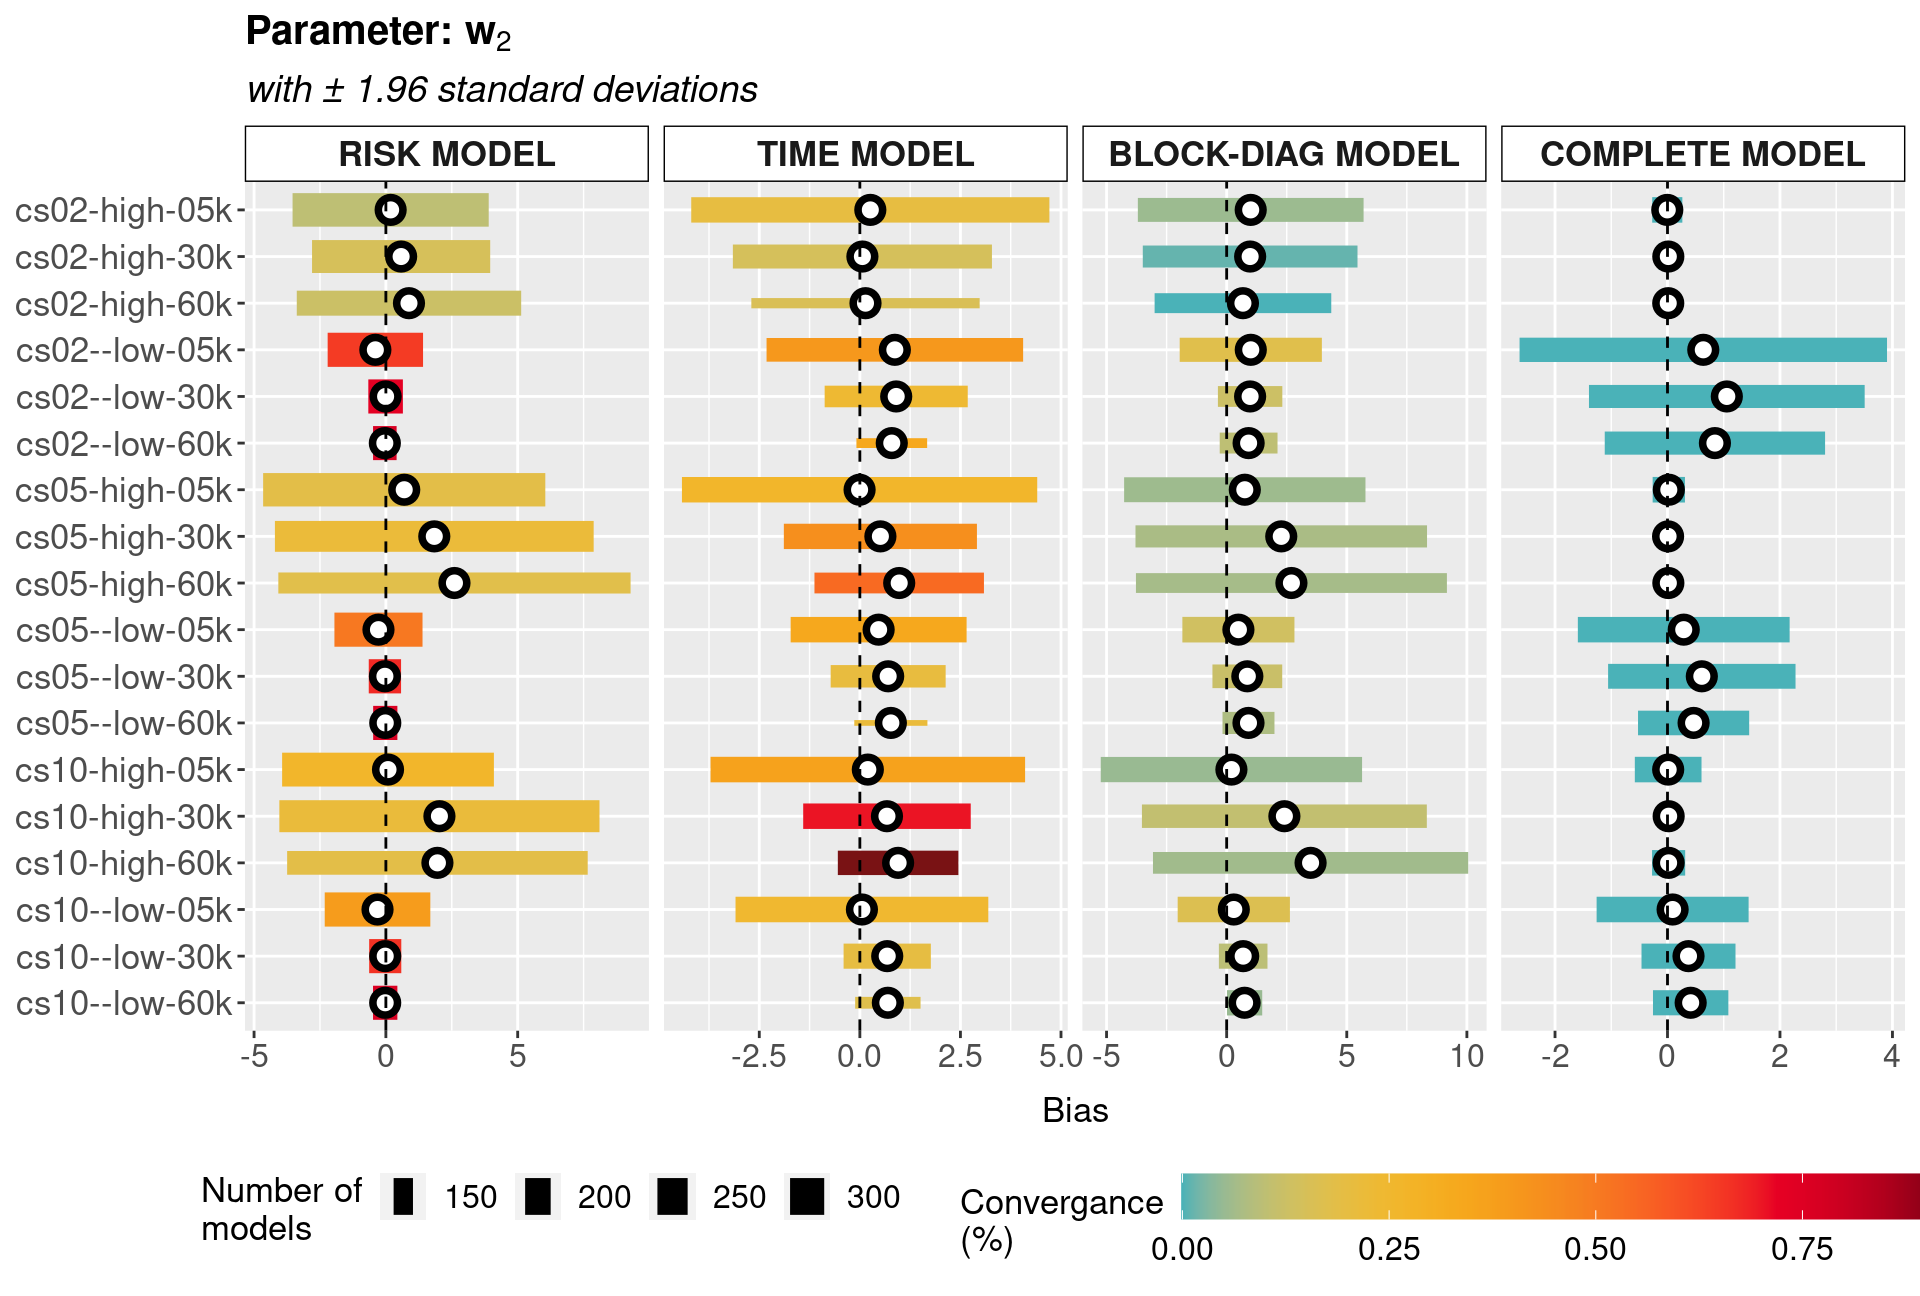
\includegraphics[width=\textwidth]{bias2plotsd-6.png}\\
 \begin{footnotesize}
  SOURCE: The author (2021).
 \end{footnotesize}
 \label{fig:biassdw2}
\end{figure}

\begin{figure}[H]
 \setlength{\abovecaptionskip}{.0001pt}
 \caption{PARAMETER \(\log(\sigma_{1}^{2})\) BIAS WITH \(\pm\) 1.96
          STANDARD DEVIATIONS}
 \vspace{0.2cm}\centering
 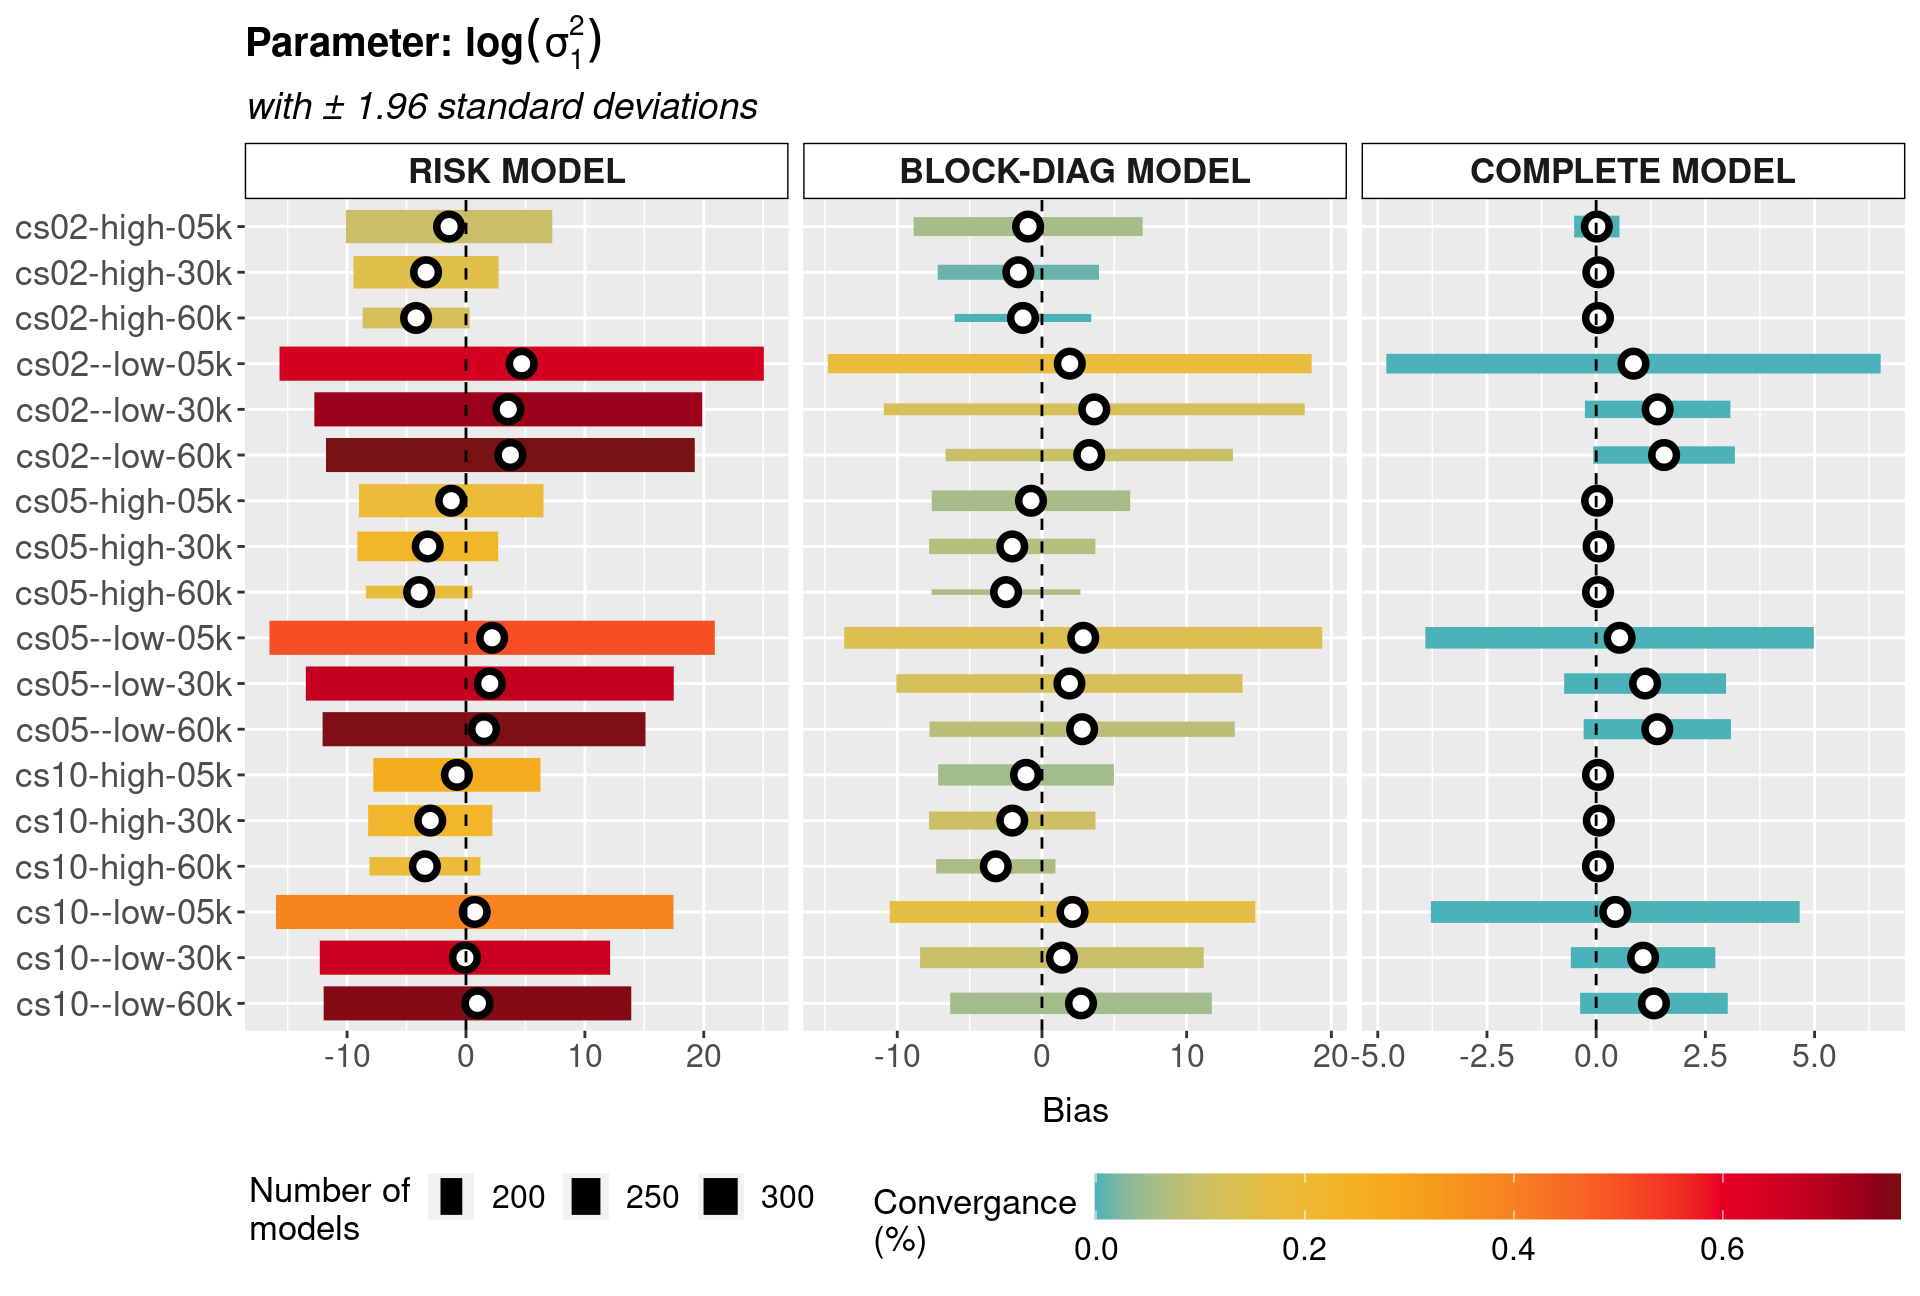
\includegraphics[width=\textwidth]{bias2plotsd-7.png}\\
 \begin{footnotesize}
  SOURCE: The author (2021).
 \end{footnotesize}
 \label{fig:biassdlogs2_1}
\end{figure}

\begin{figure}[H]
 \setlength{\abovecaptionskip}{.0001pt}
 \caption{PARAMETER \(\log(\sigma_{2}^{2})\) BIAS WITH \(\pm\) 1.96
          STANDARD DEVIATIONS}
 \vspace{0.2cm}\centering
 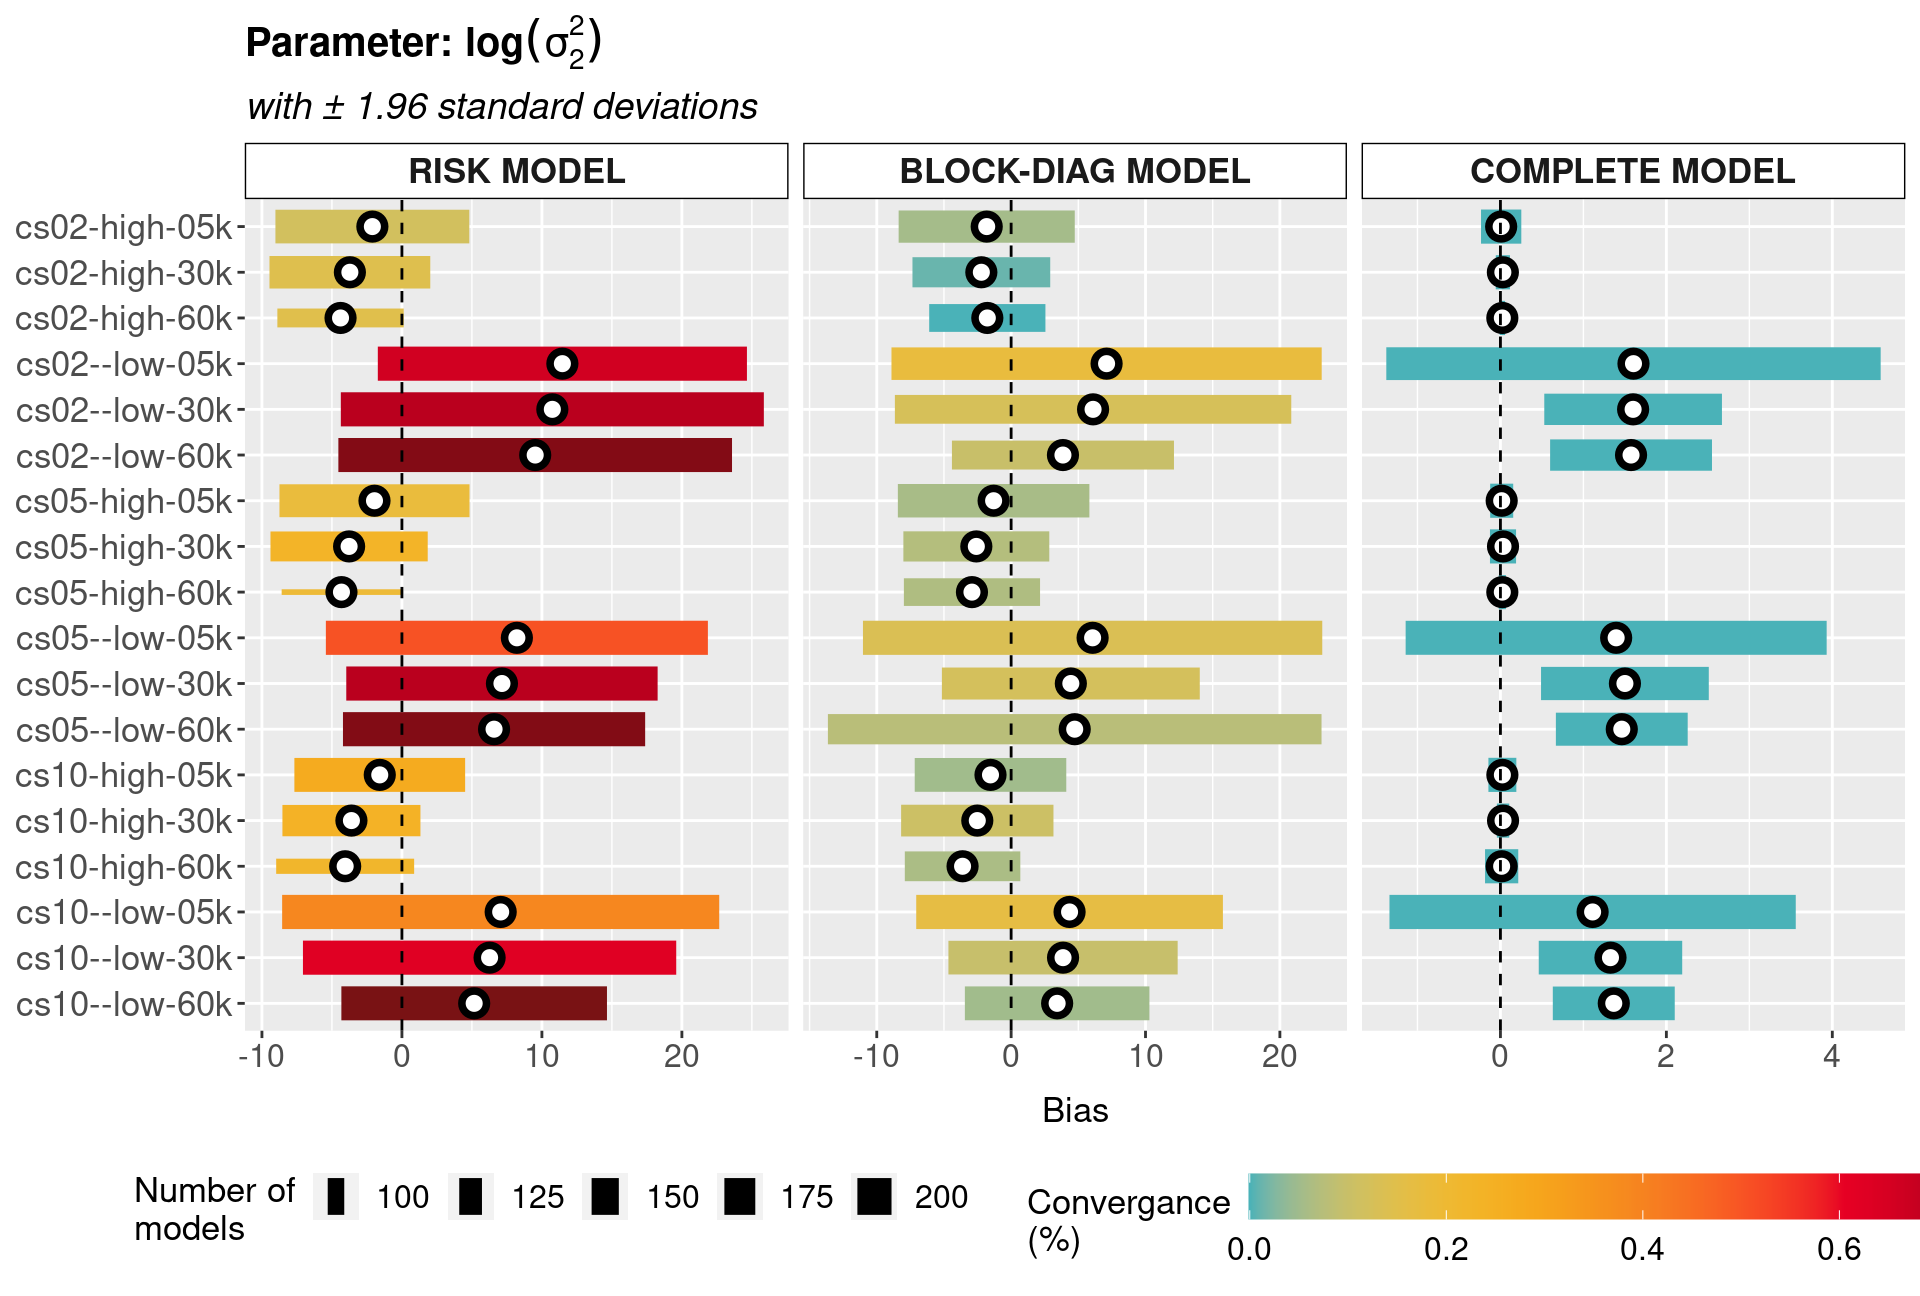
\includegraphics[width=\textwidth]{bias2plotsd-8.png}\\
 \begin{footnotesize}
  SOURCE: The author (2021).
 \end{footnotesize}
 \label{fig:biassdlogs2_2}
\end{figure}

\begin{figure}[H]
 \setlength{\abovecaptionskip}{.0001pt}
 \caption{PARAMETER \(\log(\sigma_{3}^{2})\) BIAS WITH \(\pm\) 1.96
          STANDARD DEVIATIONS}
 \vspace{0.2cm}\centering
 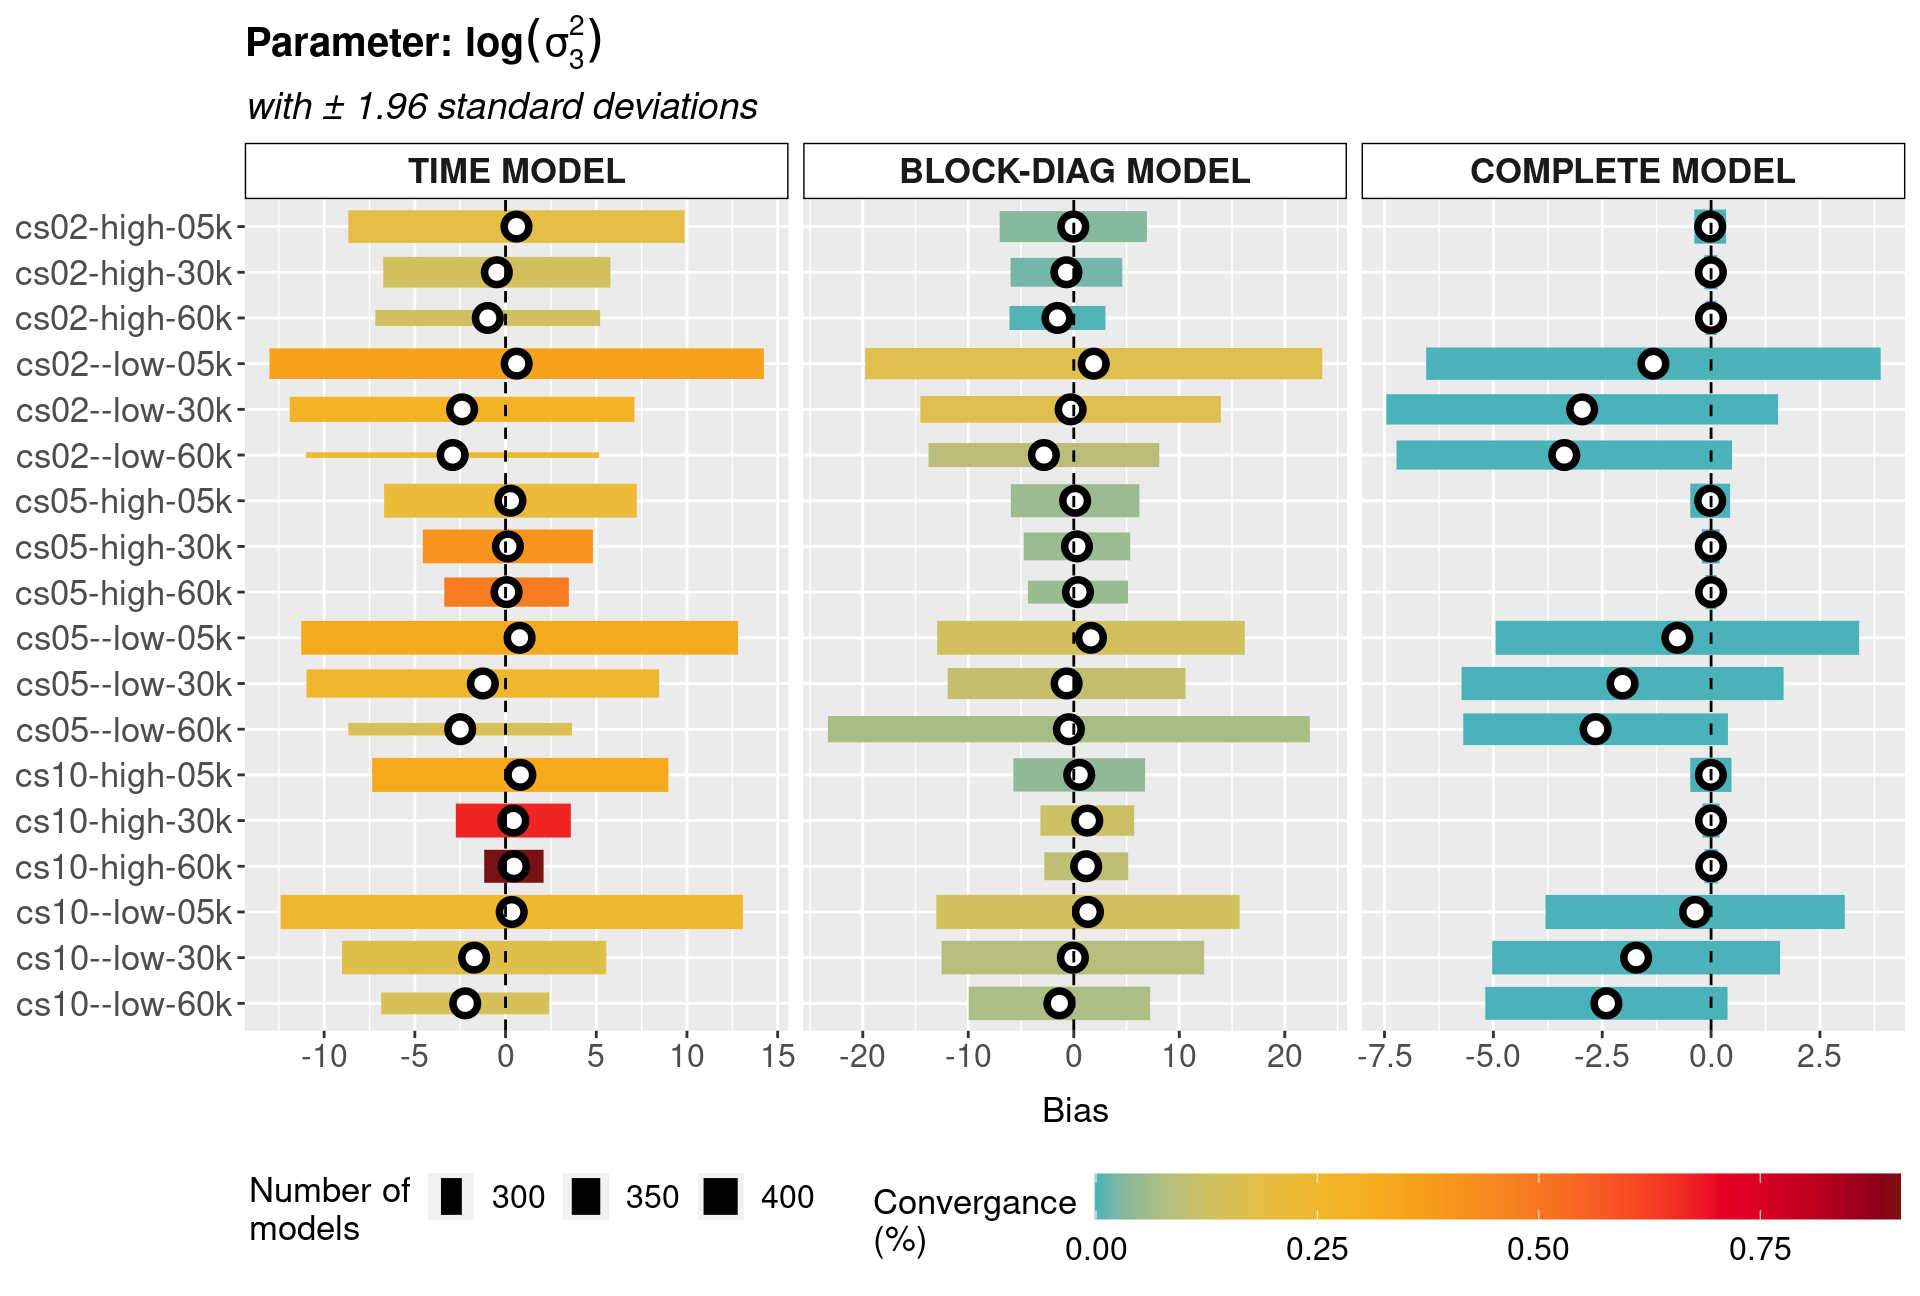
\includegraphics[width=\textwidth]{bias2plotsd-9.png}\\
 \begin{footnotesize}
  SOURCE: The author (2021).
 \end{footnotesize}
 \label{fig:biassdlogs2_3}
\end{figure}

\begin{figure}[H]
 \setlength{\abovecaptionskip}{.0001pt}
 \caption{PARAMETER \(\log(\sigma_{4}^{2})\) BIAS WITH \(\pm\) 1.96
          STANDARD DEVIATIONS}
 \vspace{0.2cm}\centering
 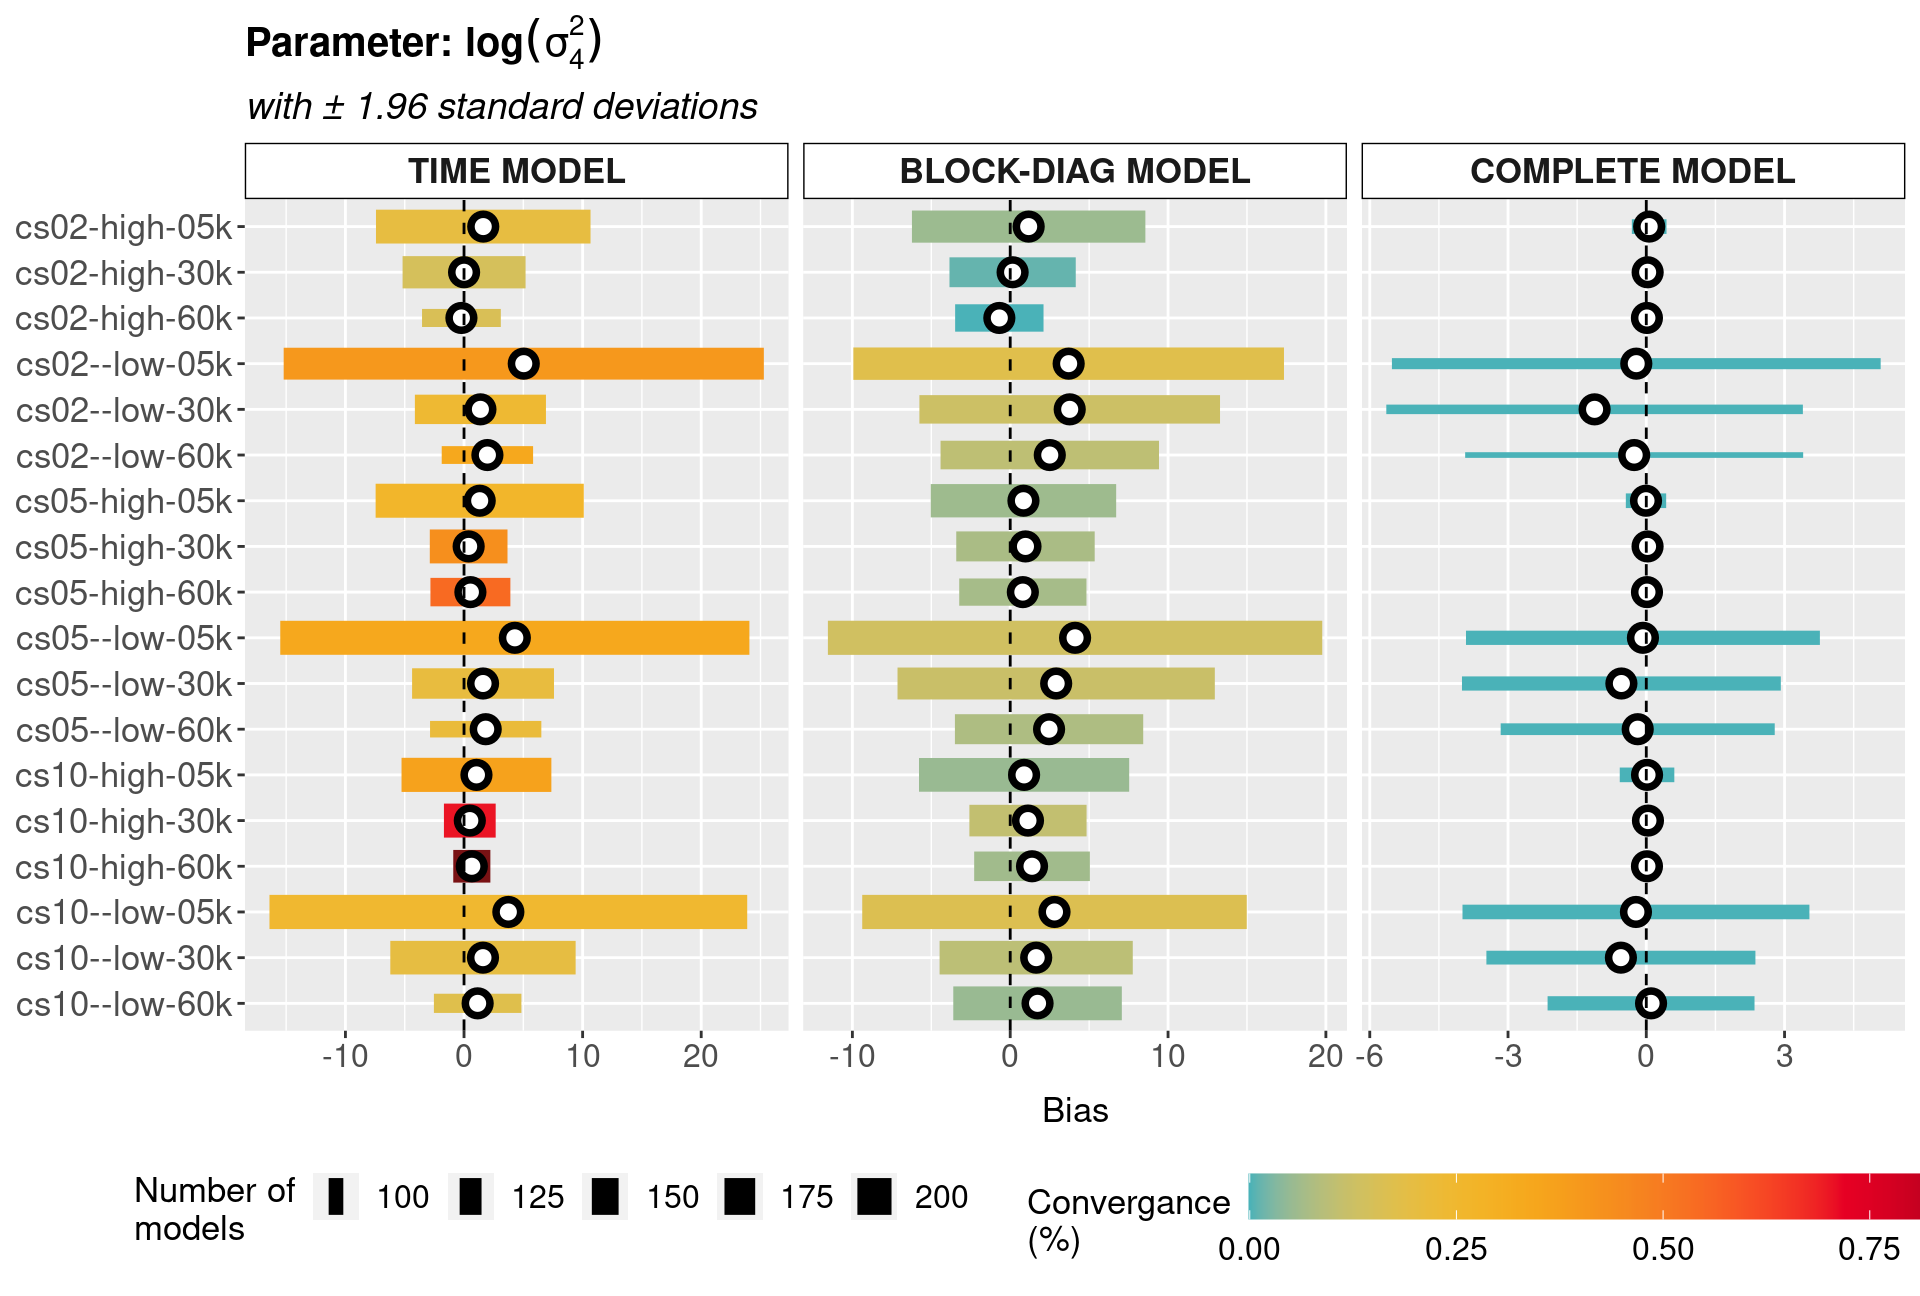
\includegraphics[width=\textwidth]{bias2plotsd-10.png}\\
 \begin{footnotesize}
  SOURCE: The author (2021).
 \end{footnotesize}
 \label{fig:biassdlogs2_4}
\end{figure}

\begin{figure}[H]
 \setlength{\abovecaptionskip}{.0001pt}
 \caption{PARAMETER \(z(\rho_{12})\) BIAS WITH \(\pm\) 1.96 STANDARD
          DEVIATIONS}
 \vspace{0.2cm}\centering
 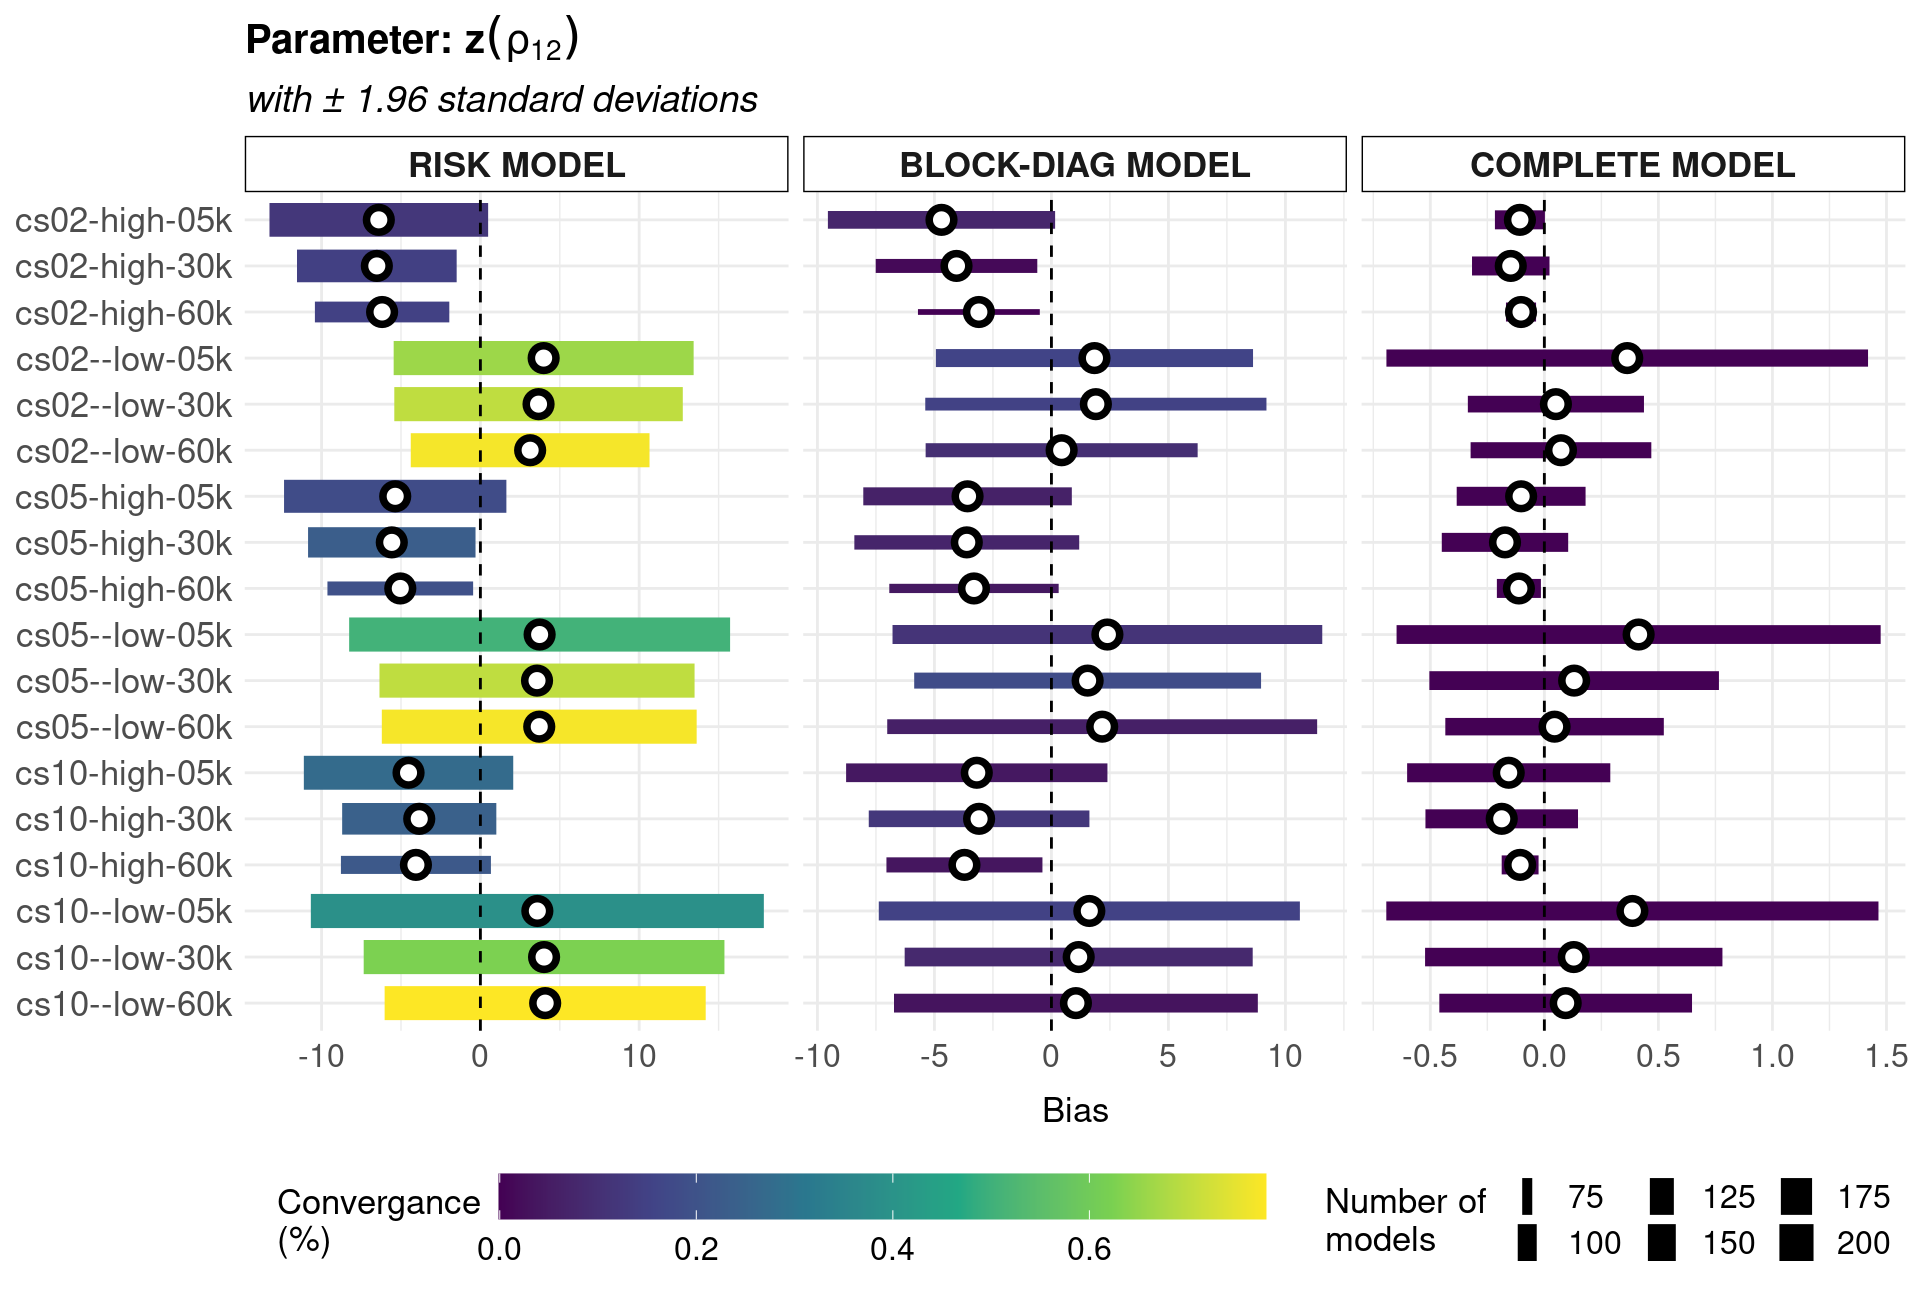
\includegraphics[width=\textwidth]{bias2plotsd-11.png}\\
 \begin{footnotesize}
  SOURCE: The author (2021).
 \end{footnotesize}
 \label{fig:biassdrhoz12}
\end{figure}

\begin{figure}[H]
 \setlength{\abovecaptionskip}{.0001pt}
 \caption{PARAMETER \(z(\rho_{34})\) BIAS WITH \(\pm\) 1.96 STANDARD
          DEVIATIONS}
 \vspace{0.2cm}\centering
 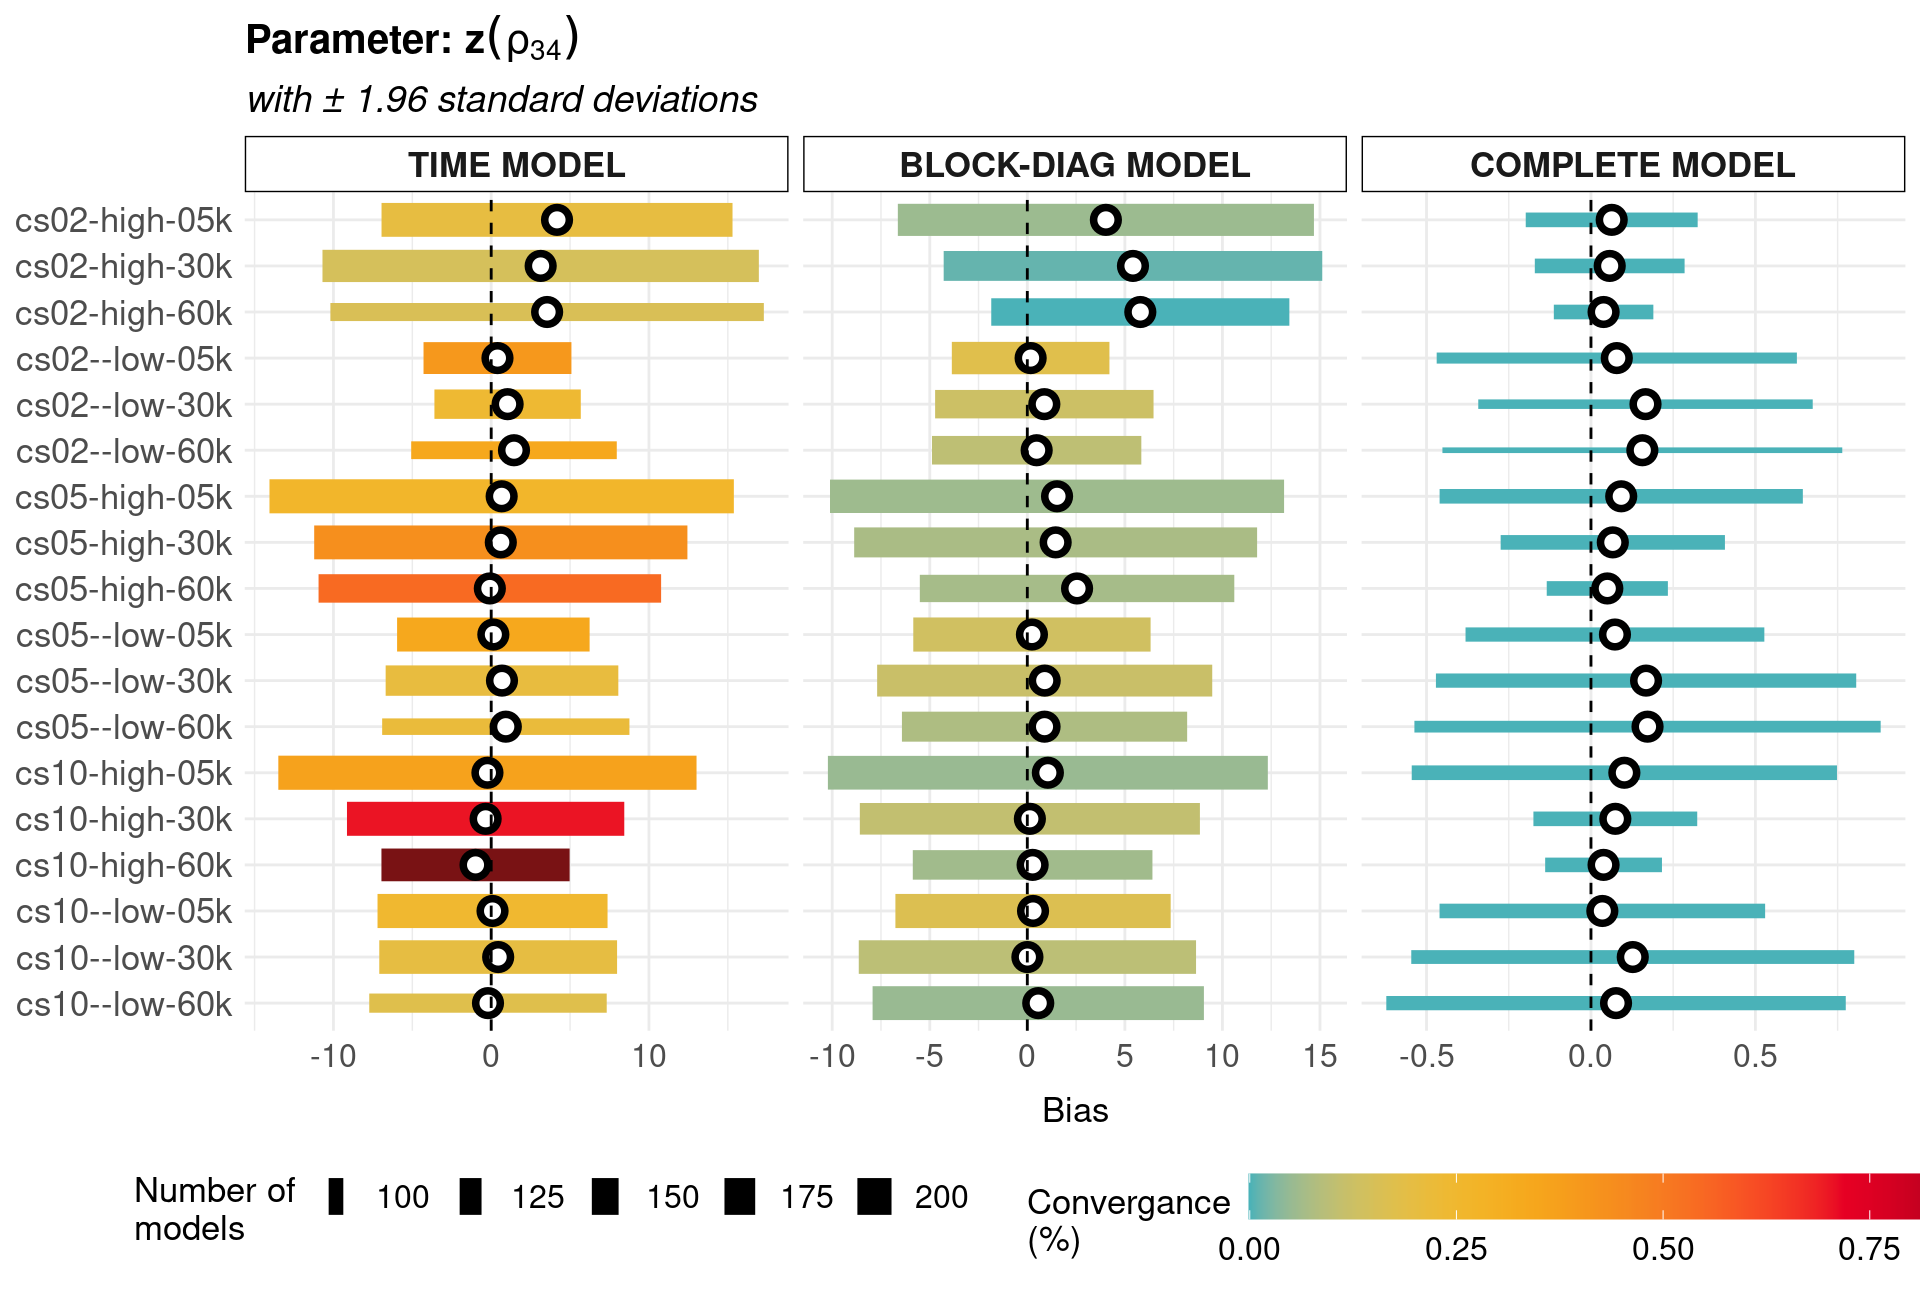
\includegraphics[width=\textwidth]{bias2plotsd-12.png}\\
 \begin{footnotesize}
  SOURCE: The author (2021).
 \end{footnotesize}
 \label{fig:biassdrhoz34}
\end{figure}

\begin{figure}[H]
 \setlength{\abovecaptionskip}{.0001pt}
 \caption{PARAMETERS
          \(\{z(\rho_{13}),~z(\rho_{24}),~z(\rho_{14}),~z(\rho_{23})\}\)
          BIAS WITH \(\pm\) 1.96 STANDARD DEVIATIONS}
 \vspace{0.2cm}\centering
 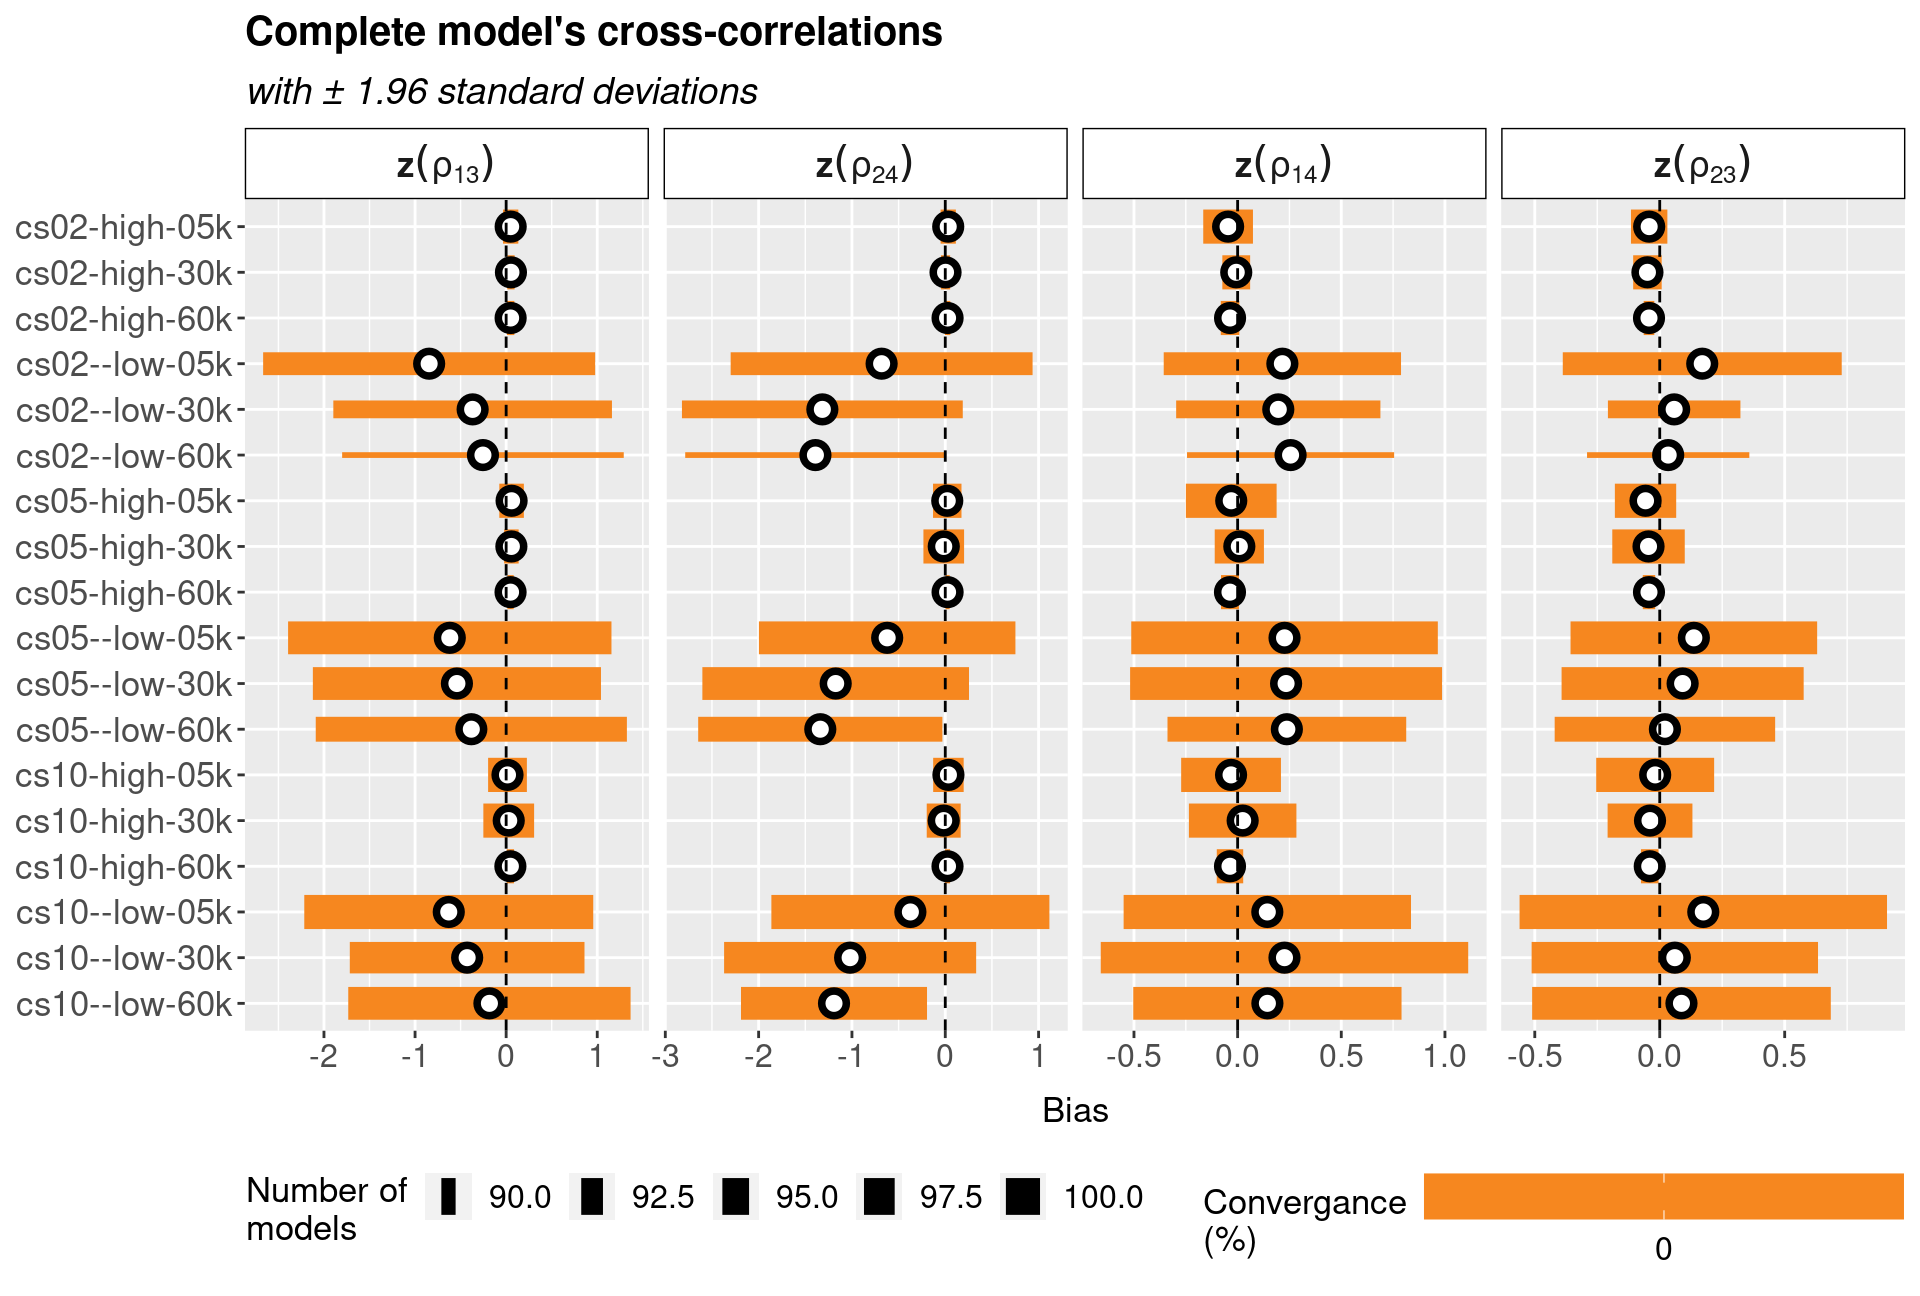
\includegraphics[width=\textwidth]{bias2plotsd-13.png}\\
 \begin{footnotesize}
  SOURCE: The author (2021).
 \end{footnotesize}
 \label{fig:biassdrhoz4}
\end{figure}

In each figure, we have the parameter bias and its uncertainty described
by a Wald-based interval i.e., \(\pm\) 1.96 the bias standard
deviation. This is a good uncertainty representation choice since it is
symmetric and robust to outliers. In the \autoref{cap:appendixD}, we
have the same parameters bias but with the corresponding 2.5 and 97.5\%
quantiles.

The seventy-two scenarios are accommodated. We have up to four blocks of
bars, each block representing a model. In each block we have eighteen
bars, each bar representing the 300 fits in each of the eighteen
scenarios (\(4 \times 18 \times 300 = 21600\)). Each scenario name
consists of a combination of three strings. The cluster size (cs), 2, 5,
and 10; the CIF configuration, high and low; the sample size, 5, 30, and
60 thousand. We have tried to fit a total of 21600 models but not all
converged. Besides that inconvenience, from the ones that converged do
not all converged in the strict sense of the word. To show these two
characteristics respectively, we control the bar widths and colors.

The ideal convergence is the traditional one i.e., based on the
gradient. However, in complicated optimization scenarios as the one we
are here, we can reach a convergence based on a metric different from
the gradient one.

In \texttt{base::nlmimb()} \texttt{R}'s \texttt{PORT} implementation,
when the default gradient-based convergence is reached we get a 0
message. When the optimization converges but not gradient-based, we get
a 1 message. Looking at the technical report of \citeonline{PORTreport},
we see that this convergence style means that the last algorithm iterate
\(x\) appears to be at a certain scaled distance of the locally optimal
point \(x^{\ast}\). This scaled distance, \(p(x, x^{\ast})\), is defined
by
\[
 p(x, y) =
 \underset{1~\leq i~\leq~p}{\text{max}}
 \left\{d_{i}, |x_{i} - y_{i}|\right\}
 \Big/
 \underset{1~\leq j~\leq~p}{\text{max}}
 \left\{d_{j}, |x_{j}| + |y_{j}|\right\},
\]
where \(d\) is a certain scale vector. In all figures, the considered
convergence percentage is from the gradient-based one.

Something specific can be said about each parameter but let us keep the
focus on the general remarks. Starting from the fixed-effect parameters
(\autoref{fig:biassdbeta1}, \autoref{fig:biassdbeta2},
\autoref{fig:biassdgama1}, \autoref{fig:biassdgama2},
\autoref{fig:biassdw1}, \autoref{fig:biassdw2}), we have some very nice
results that already show a strong inclination to the complete model's
choice.

With a simpler latent structure i.e., a latent structure only in one
level (risk and time models), the low CIF scenarios present a much
smaller bias-variance. In general, the mean-bias is small (good), but
the variances are high. When we have a latent structure on both levels
but assuming the cross-correlations as zero (block-diag model), the
results get a little bit better. Nevertheless, when we assume a non-zero
cross-correlation structure (complete model) basically everything
changes. The mean biases get closer to zero, the standard deviations
decrease 50\% or more, and mainly, now the high CIF scenarios are the
ones with a much smaller bias-variance. All this is accomplished through
the consideration of the cross-correlations.

In the \textit{simpler} models is hard to see some significant
difference between the cluster and sample sizes. In the complete model,
the difference is clear: as we increase the cluster and the sample size
the bias-variance decrease. The mean-bias is basically always the
same. In the risk and block-diag models is hard to point-out a scenario
as the best or worst. For the time model, in two parameters, with the
scenario of cluster size ten; low CiF; and five thousand data points, we
get a much bigger standard deviation.

With the log-variances (\autoref{fig:biassdlogs2_1},
\autoref{fig:biassdlogs2_2}, \autoref{fig:biassdlogs2_3},
\autoref{fig:biassdlogs2_4}), we have instead a similar behavior through
the models. For all models, the high CIF scenarios are the ones with a
smaller mean and bias-variance. From the risk/time model to the
block-diag model, we do not see a significant improvement in terms of
bias reduction. Such improvement, however, is clear when we look at the
complete model. Again, the magick of considering the cross-correlations.

The same said about the log-variances, can be applied to the risk
correlation (\autoref{fig:biassdrhoz12}) with one addendum: the bias
reduction is even bigger. With the time correlation
(\autoref{fig:biassdrhoz34}), we get the same behavior observed with the
fixed-effect parameters i.e., in the simpler models, the smaller biases
are observed with the low CIF scenarios. However, with the complete
model, we get the opposite. With the cross-correlations
(\autoref{fig:biassdrhoz4}), the mean and bias-variance are much smaller
in the high CIF scenarios.

The biggest bias-variances obtained are with the log-variances. A final
remark to be made is about convergences. With the simpler models, not
all of them work, having in some scenarios (generally the ones with
sixty thousand points) a 50\(\sim\)60\% convergence rate. However, from
this 50\(\sim\)60\%, most reach the ideal gradient-based
convergence. The complete model is the complete opposite. Basically, all
fits reach a convergence (\(\sim\)100\% performance) but never the
desired gradient-based convergence.

After looking at the parameter biases, let us take a look at the implied
mean-CIF curves. To nicely represent all seventy-two scenarios we split
the curves by level-CIF. In \autoref{fig:cifshigh} we have the high CIF
scenario curves and in \autoref{fig:cifslow} the low CIF scenario
curves.

\begin{figure}[H]
 \setlength{\abovecaptionskip}{.0001pt}
 \caption{HIGH CUMULATIVE INCIDENCE FUNCTION (CIF) SCENARIO CURVES}
 \vspace{0.2cm}\centering
 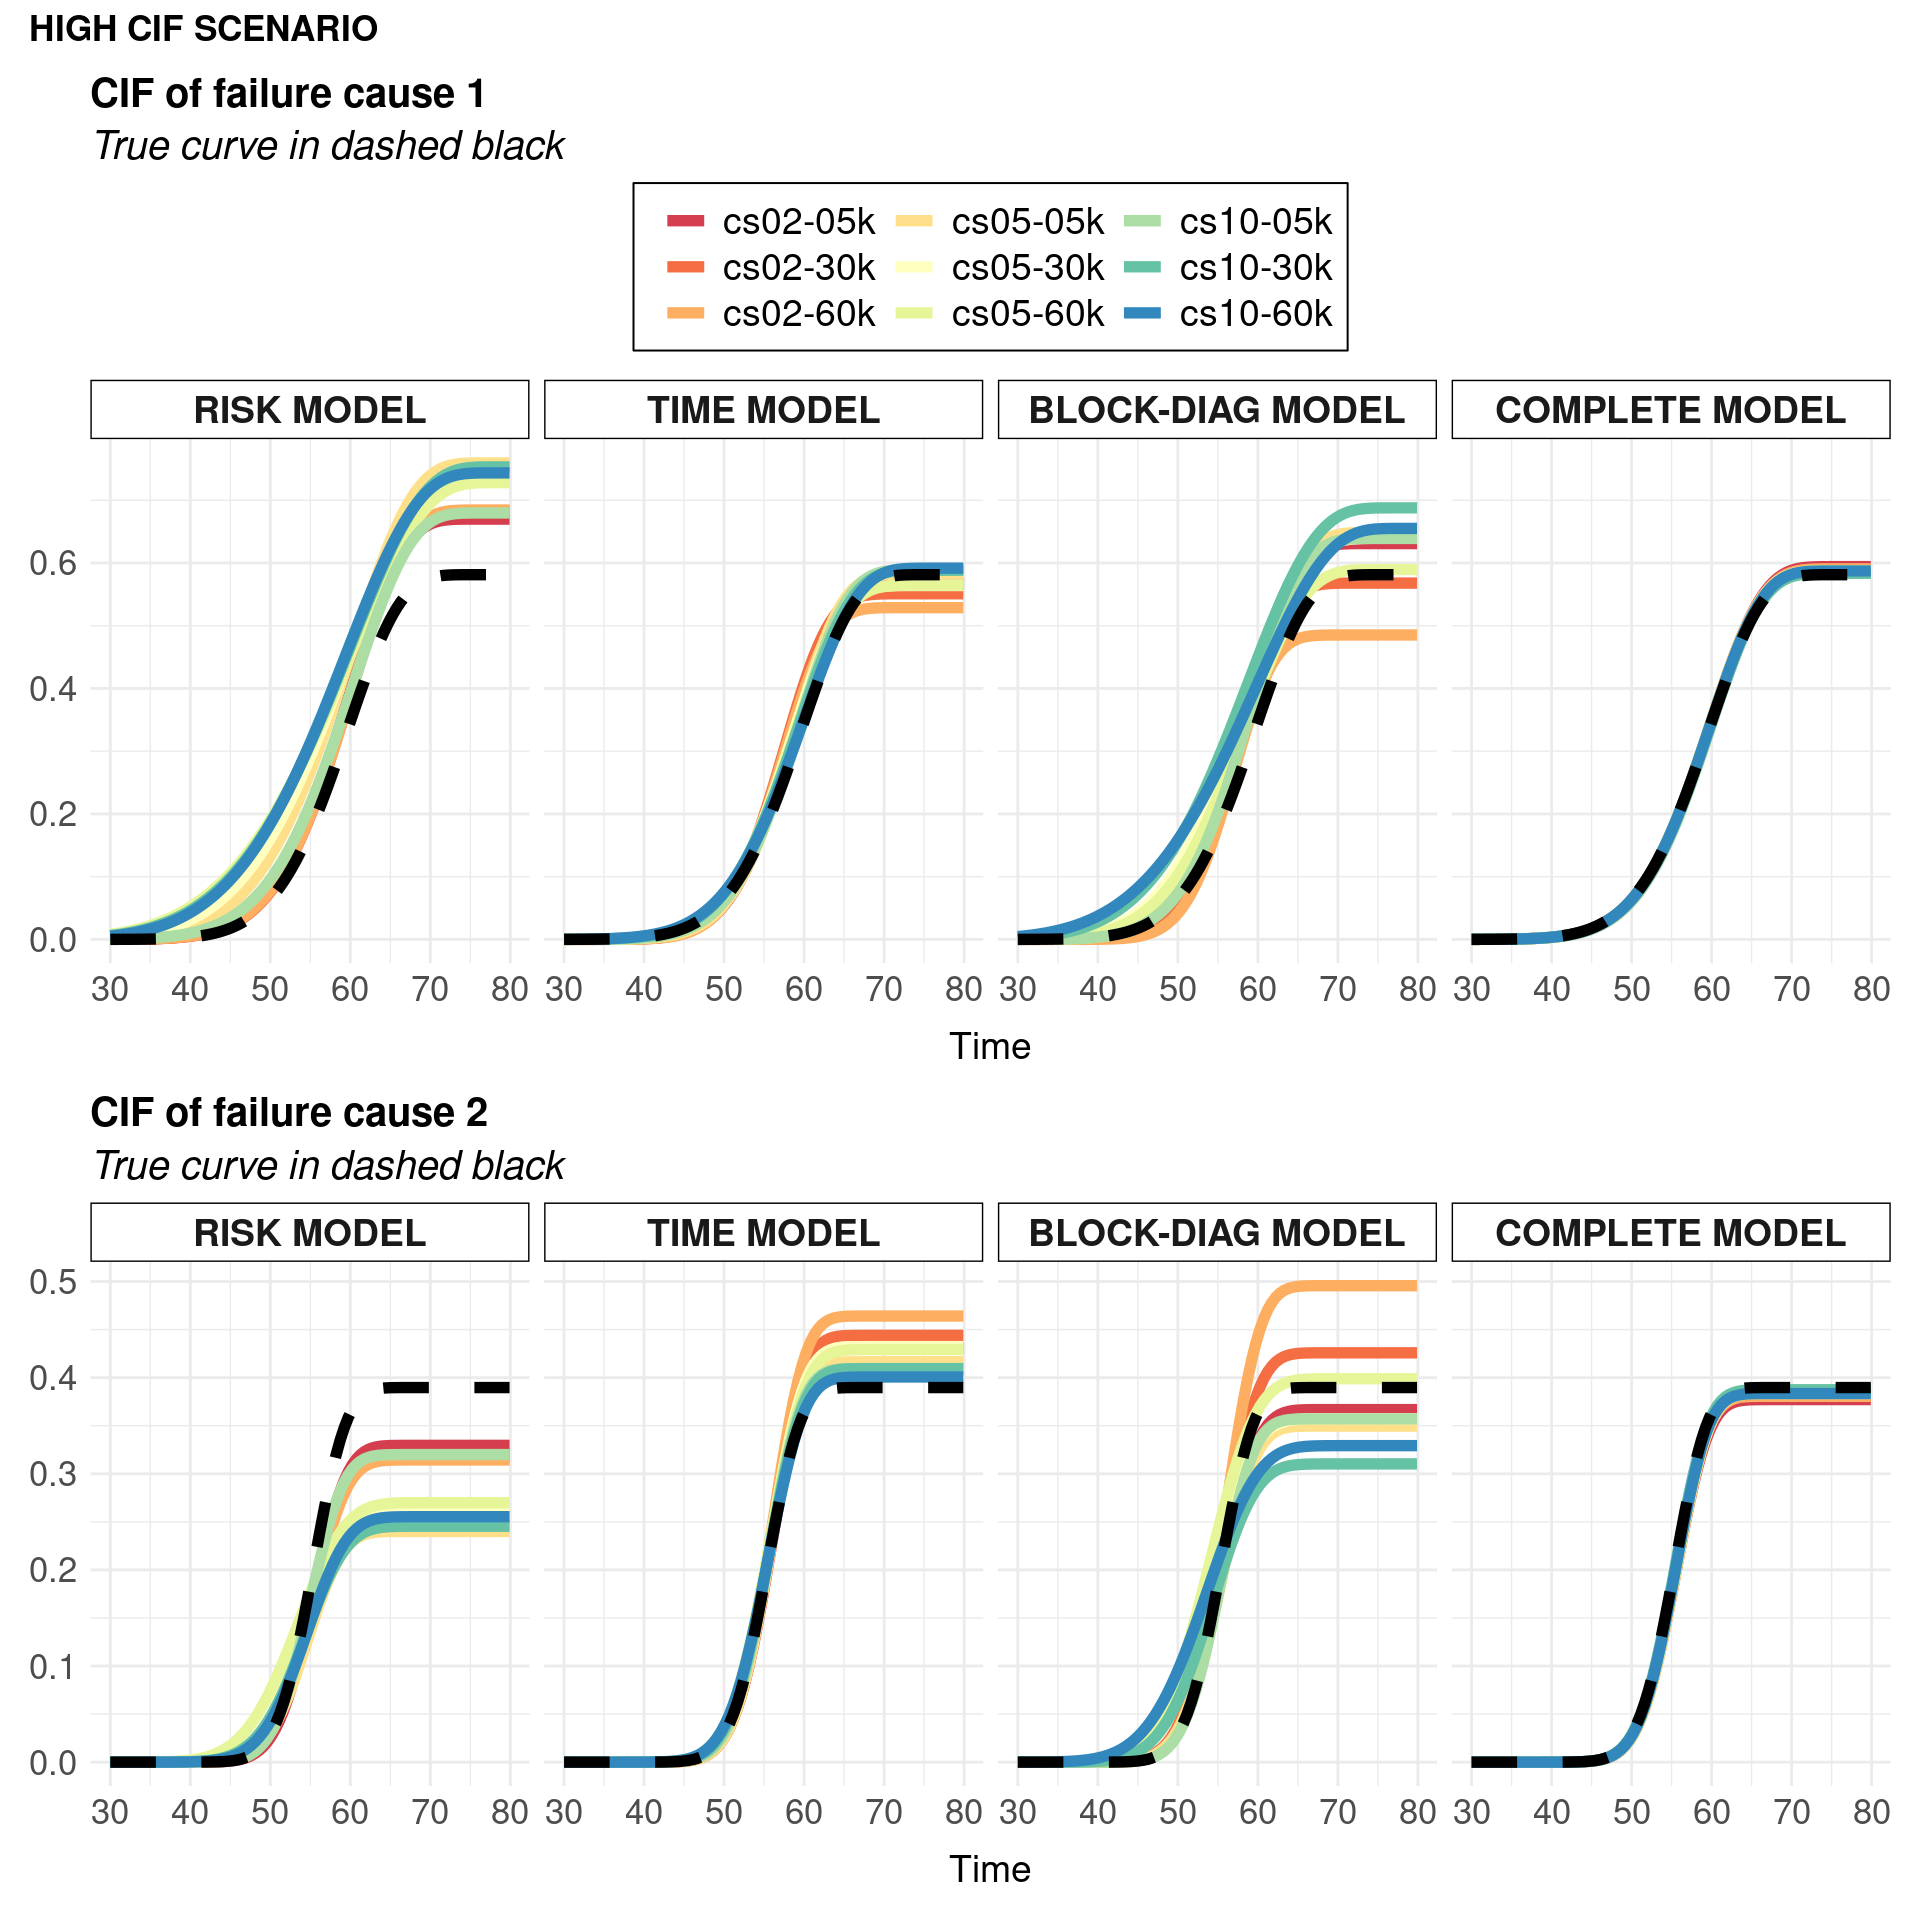
\includegraphics[width=\textwidth]{cifs-1.png}\\
 \begin{footnotesize}
  SOURCE: The author (2021).
 \end{footnotesize}
 \label{fig:cifshigh}
\end{figure}

\begin{figure}[H]
 \setlength{\abovecaptionskip}{.0001pt}
 \caption{LOW CUMULATIVE INCIDENCE FUNCTION (CIF) SCENARIO CURVES}
 \vspace{0.2cm}\centering
 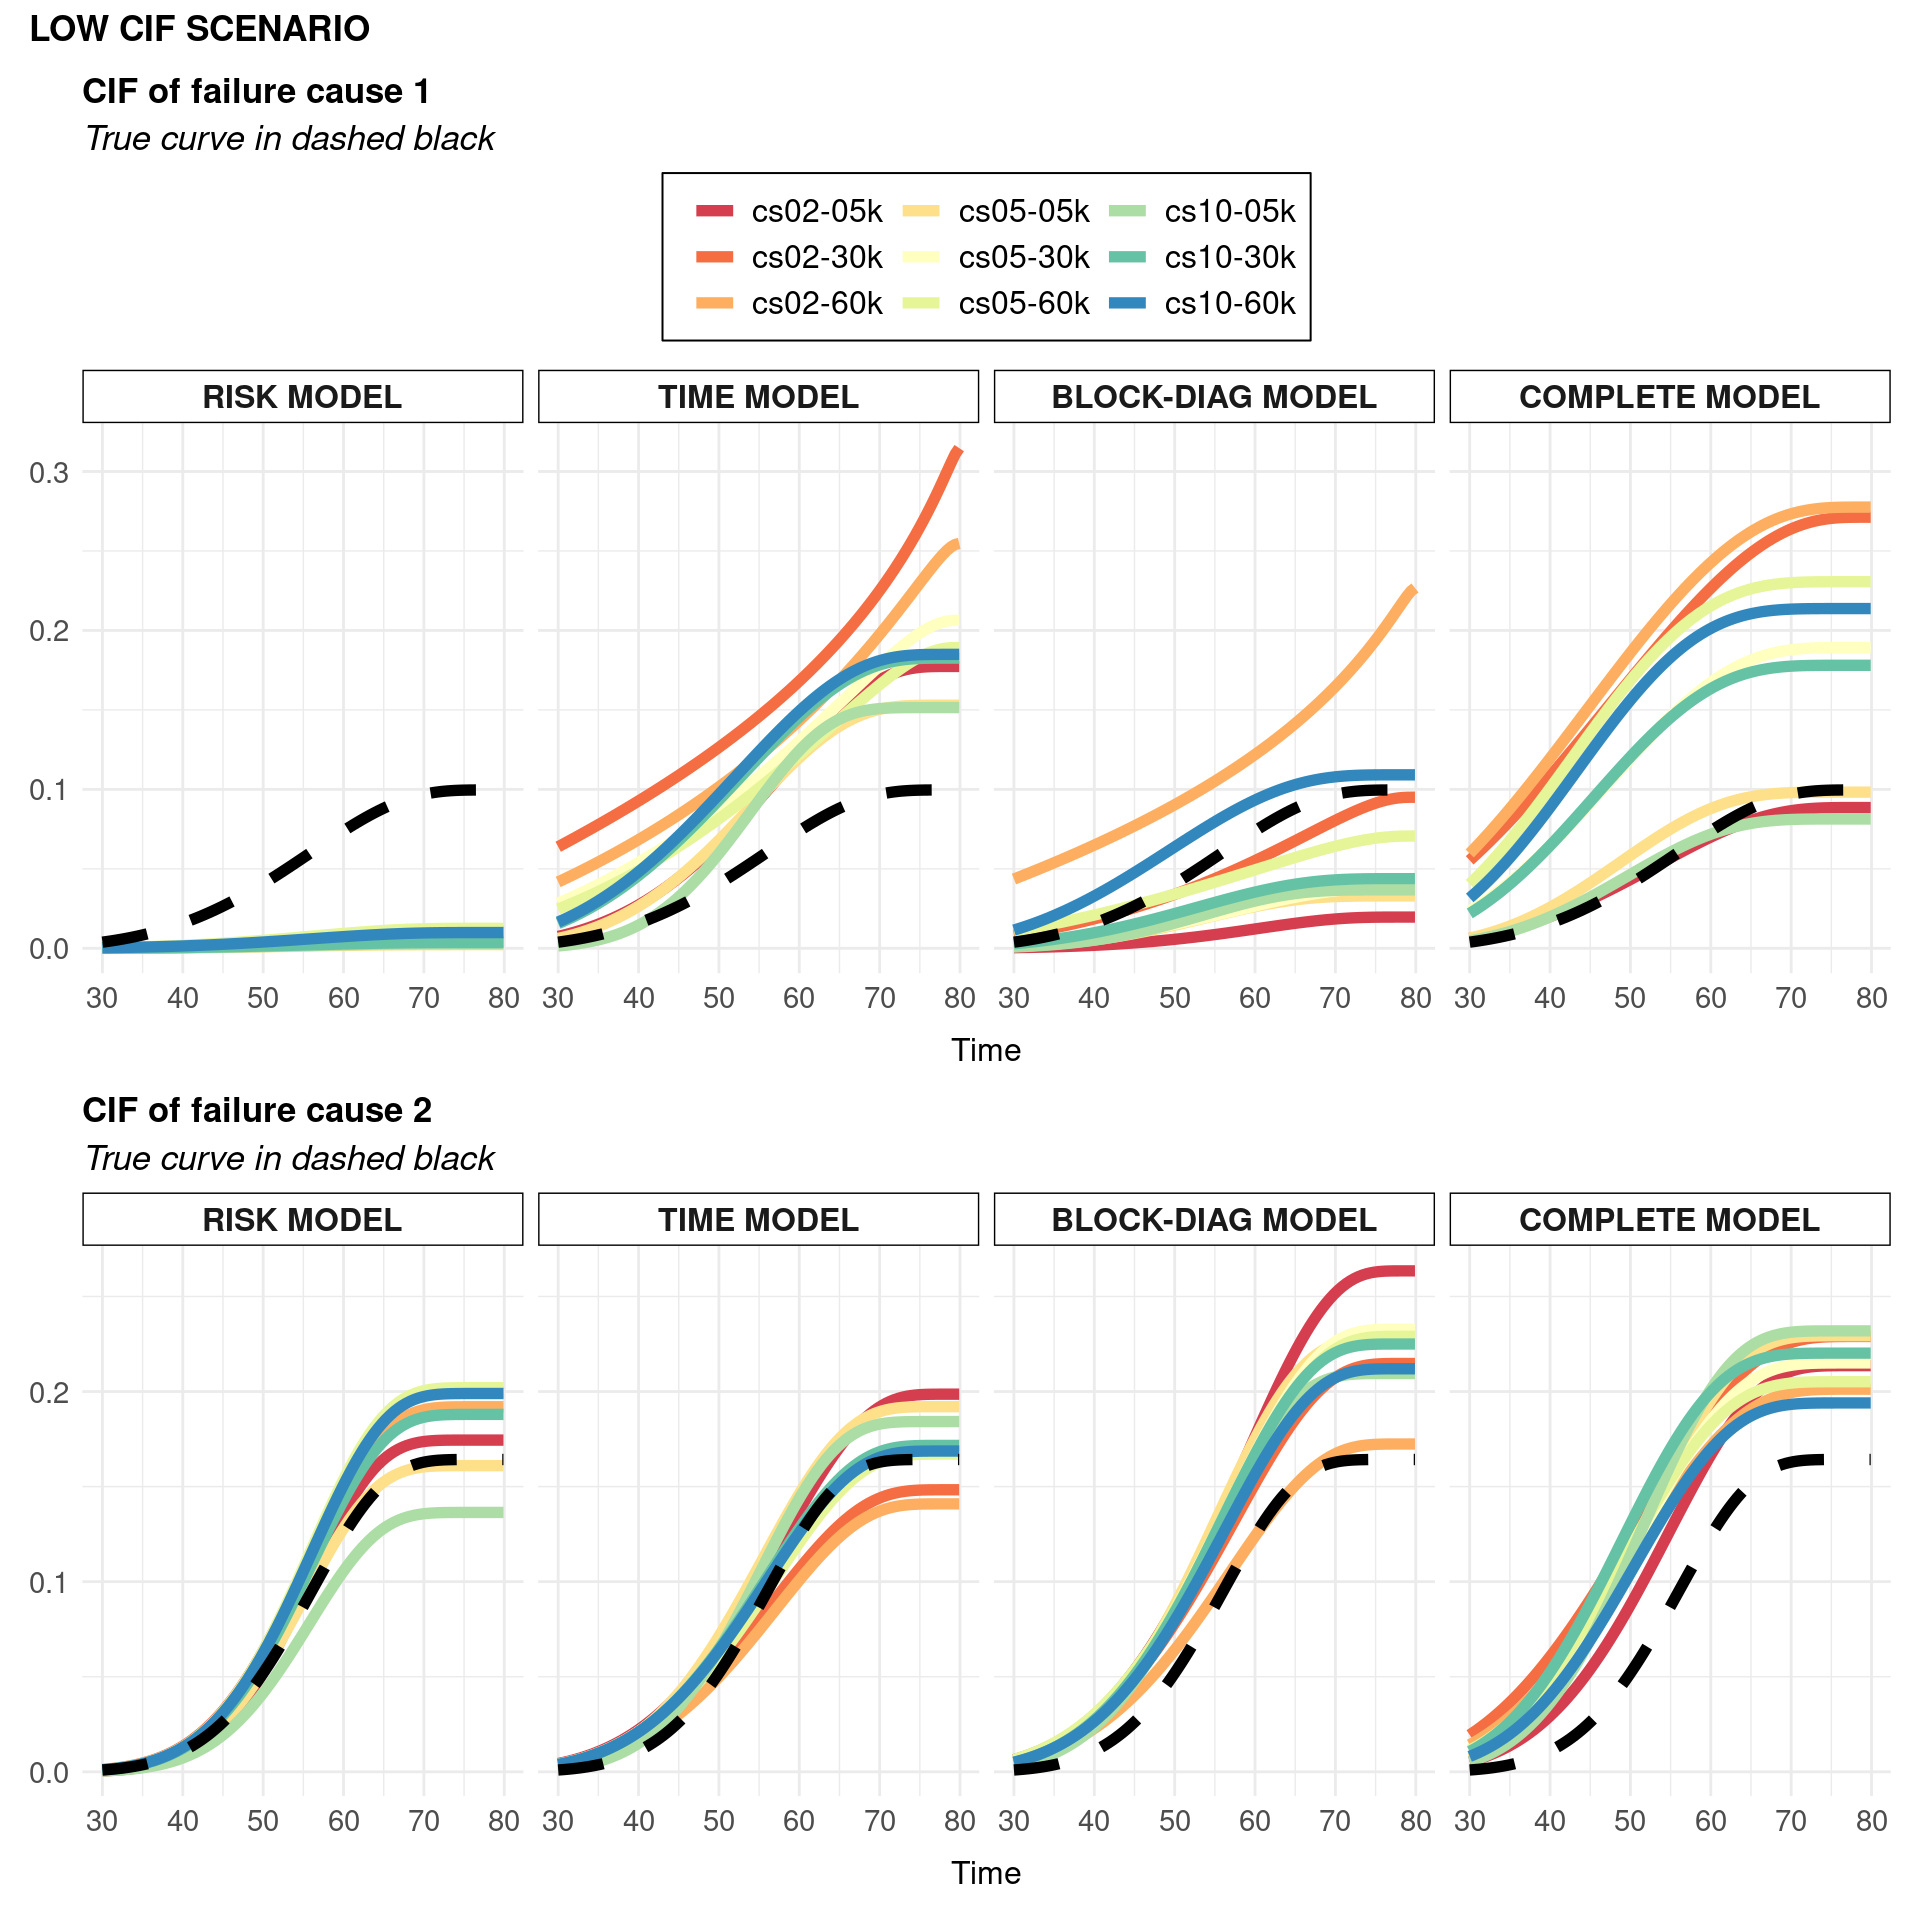
\includegraphics[width=\textwidth]{cifs-2.png}\\
 \begin{footnotesize}
  SOURCE: The author (2021).
 \end{footnotesize}
 \label{fig:cifslow}
\end{figure}

Since in all models we have a latent structure for the within-cluster
dependency, the inherent idea is that this will also affect the
fixed-effect parameter estimates. By taking the average of the
fixed-effect parameter estimates in each of the seventy-two scenarios,
we are able to construct the mean CIF curve for each scenario.

In \autoref{fig:cifshigh} we have all the thirty-six curves obtained in
the high CIF scenarios. It is clear that with the complete model we get
a perfect fit in all nine scenarios. With the risk and time models, we
get right the curve shapes but we fail to learn the max incidence. A
compensation is clear in the risk model. There is a super estimation of
\(\beta_{1}\) in all scenarios. For failure cause 2, there is a sub
estimation.

With the time model, we get much better curves than with the risk
model. The block-diag model results are a middle term between them. For
the time model, the scenario with cluster size 10 and sixty-thousand
points is a highlight. For the block-diag model, the highlight is the
scenario with cluster size 5 and thirty-thousand points.

In the low CIF scenarios in \autoref{fig:cifslow}, the estimation is
clearly more difficult. The overall fits are bad, being impossible to
select a scenario with overall good results. For one of the failure
causes, the estimation quality is not so bad. The problem is when we
look to the other. The best joint fit is still with the complete model.

By bias and CIF, the scenarios with better results are the ones with
high CIF and bigger sample sizes. Besides looking to mean bias, is
interesting to look at how the latent effect parameter estimates
distribute. In \autoref{fig:histologs2} we have the densities for the
variance parameters in each of these scenarios. In
\autoref{fig:historhoz} we have the same for correlation parameters.

An interesting result is a clear difference between the risk and time
models' covariance parameters. With the risk model, we have a clear
super estimation and a bigger variance. With the time model, we get some
nice results, given the still high variance. The block-diag model
generally performs better than the risk model and worst than the time
model. Besides the bias itself, we should also pay attention to the
values. We model the variances in the log-scale, so a value 5, in
reality, is implying a variance of \(\exp(4) = 148\) i.e., terrible. All
these problems do not sound to appear with the complete model. Great.

In the complete model, we do not see any considerable difference between
the covariance densities. However, looking back to parameters bias we
see that in general, for the complete model, when we increase the sample
size the bias-variance decreases. Thus, we chose this scenario to
compute the parameter estimates correlation. The heat-map is presented
in \autoref{fig:cor2plot}.

\begin{figure}[H]
 \setlength{\abovecaptionskip}{.0001pt}
 \caption{VARIANCE PARAMETERS DENSITIES IN THE SCENARIOS OF HIGH CIF AND
          SIXTY-THOUSAND DATA POINTS}
 \vspace{0.2cm}\centering
 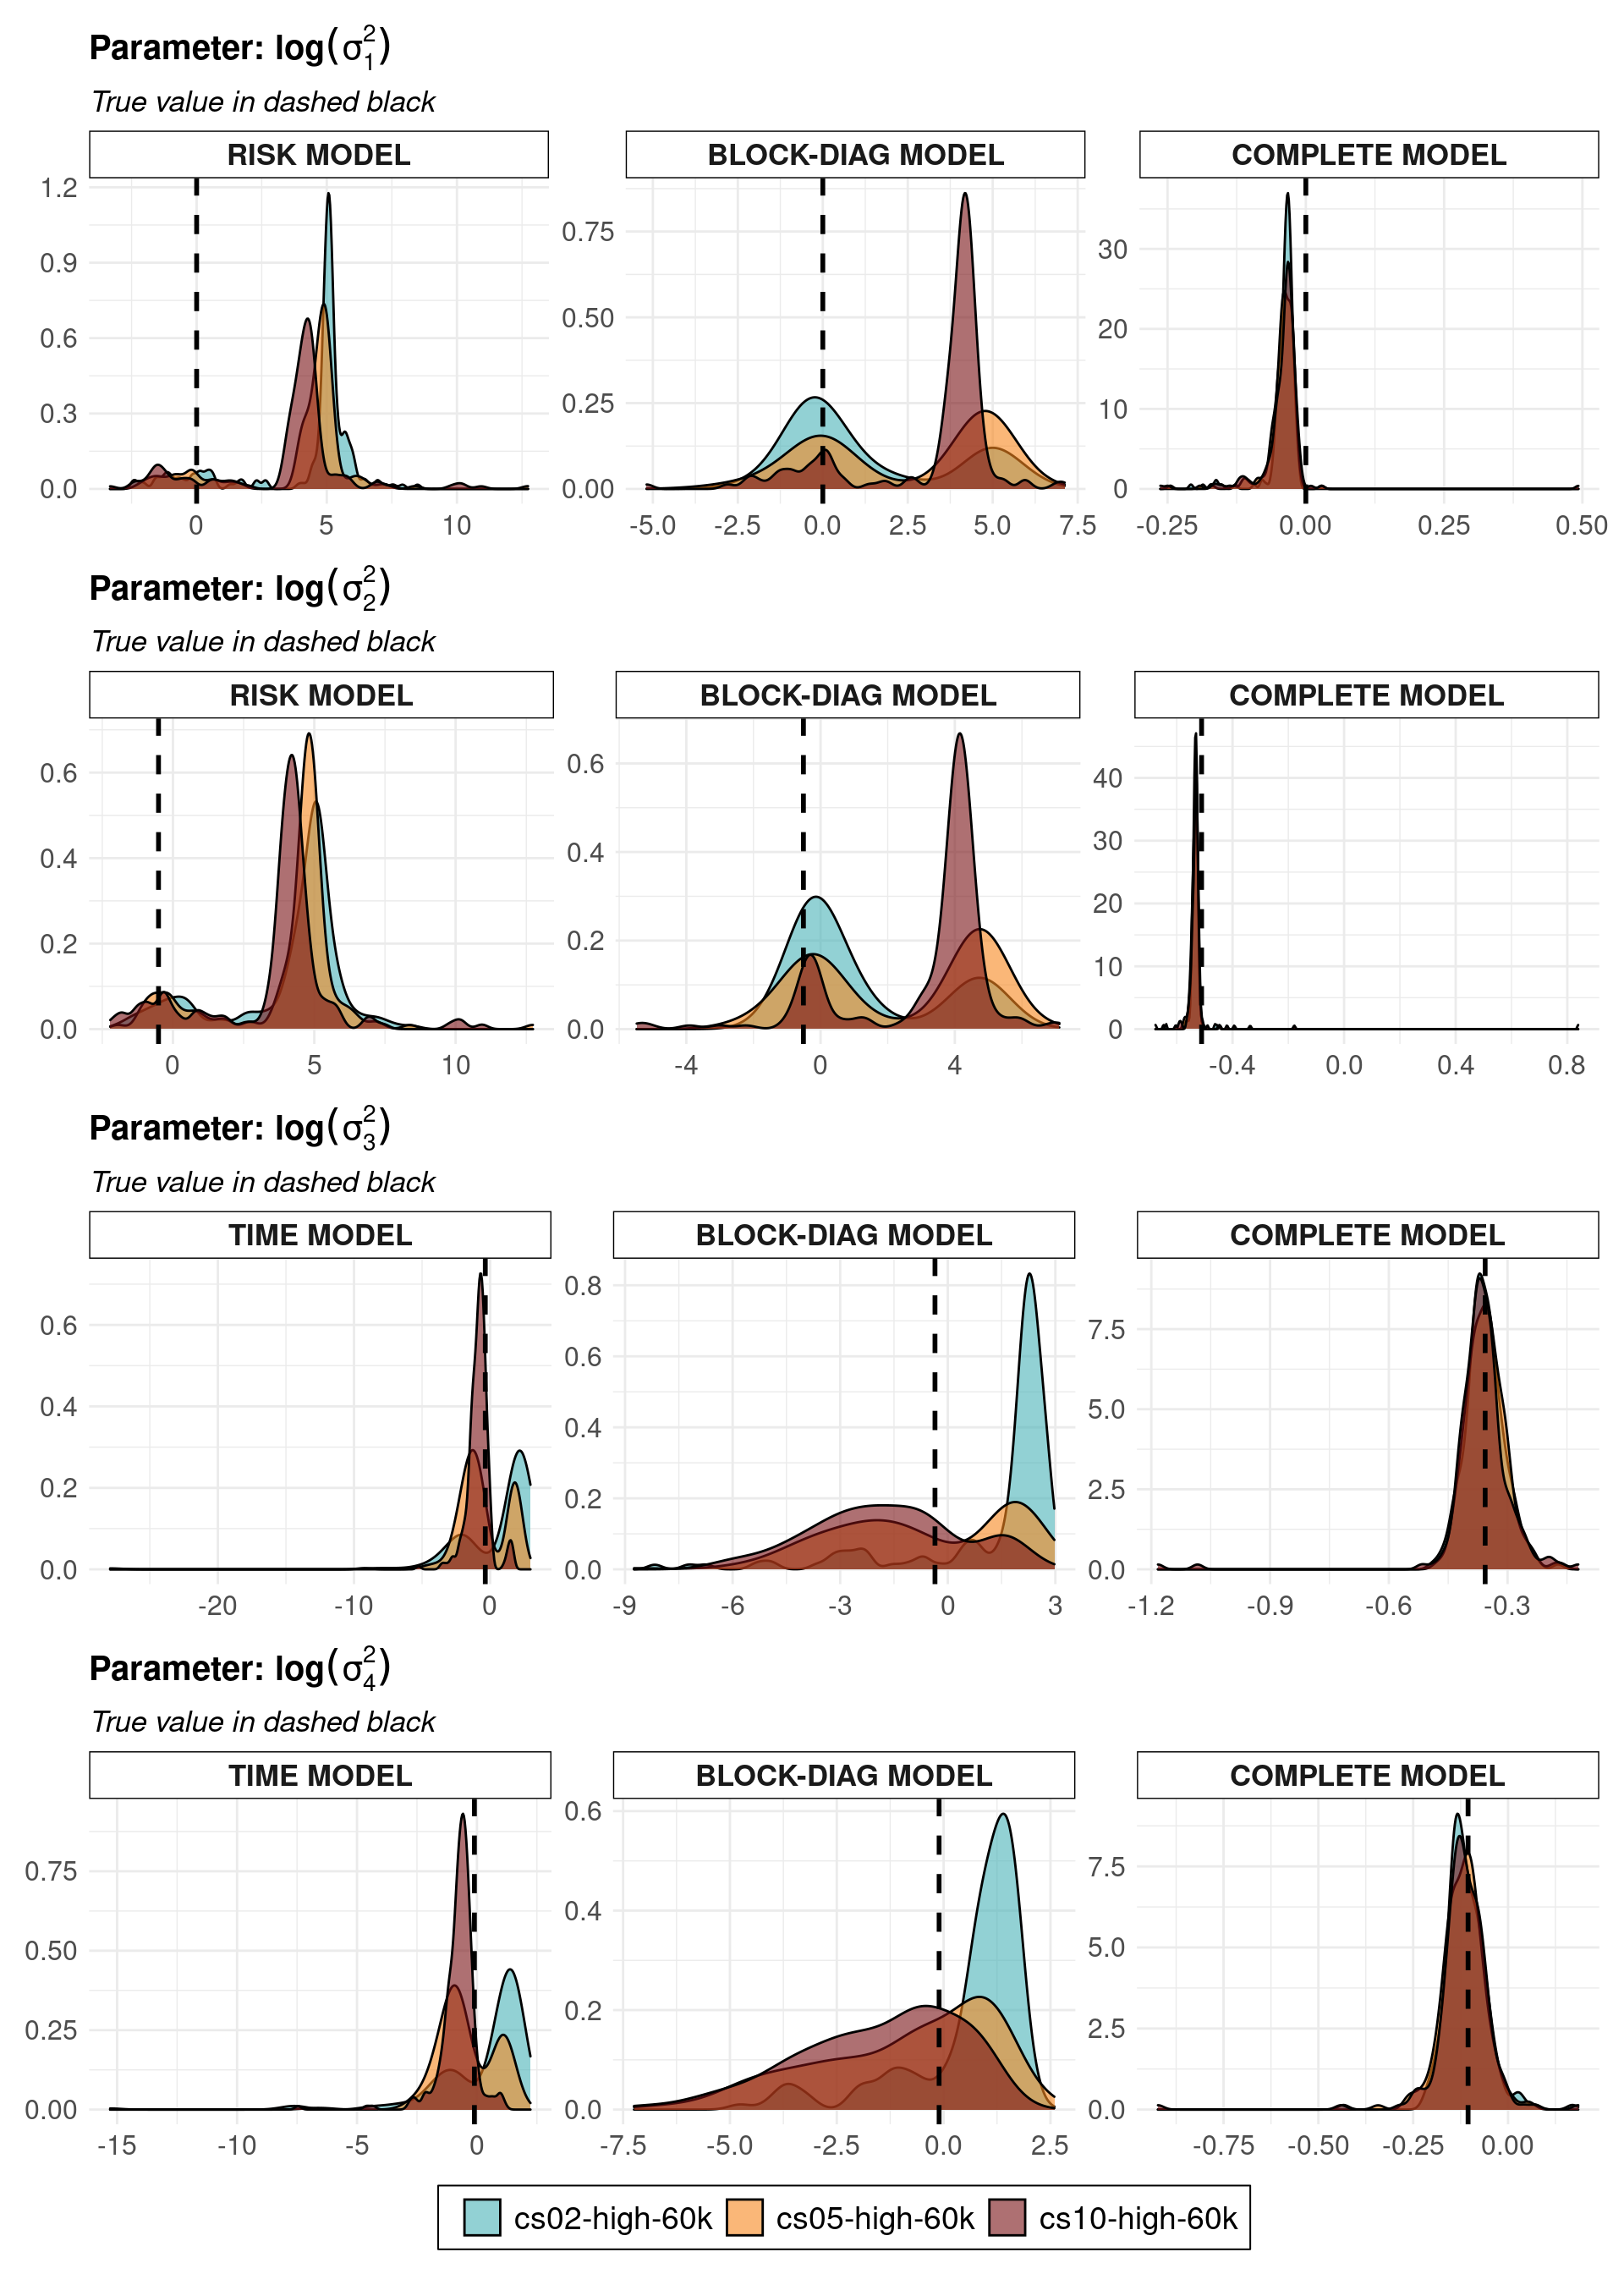
\includegraphics[width=\textwidth]{histologs2-1.png}\\
 \begin{footnotesize}
  SOURCE: The author (2021).
 \end{footnotesize}
 \label{fig:histologs2}
\end{figure}

\begin{figure}[H]
 \setlength{\abovecaptionskip}{.0001pt}
 \caption{CORRELATION PARAMETERS DENSITIES IN THE SCENARIOS OF HIGH CIF
          AND SIXTY-THOUSAND DATA POINTS}
 \vspace{0.2cm}\centering
 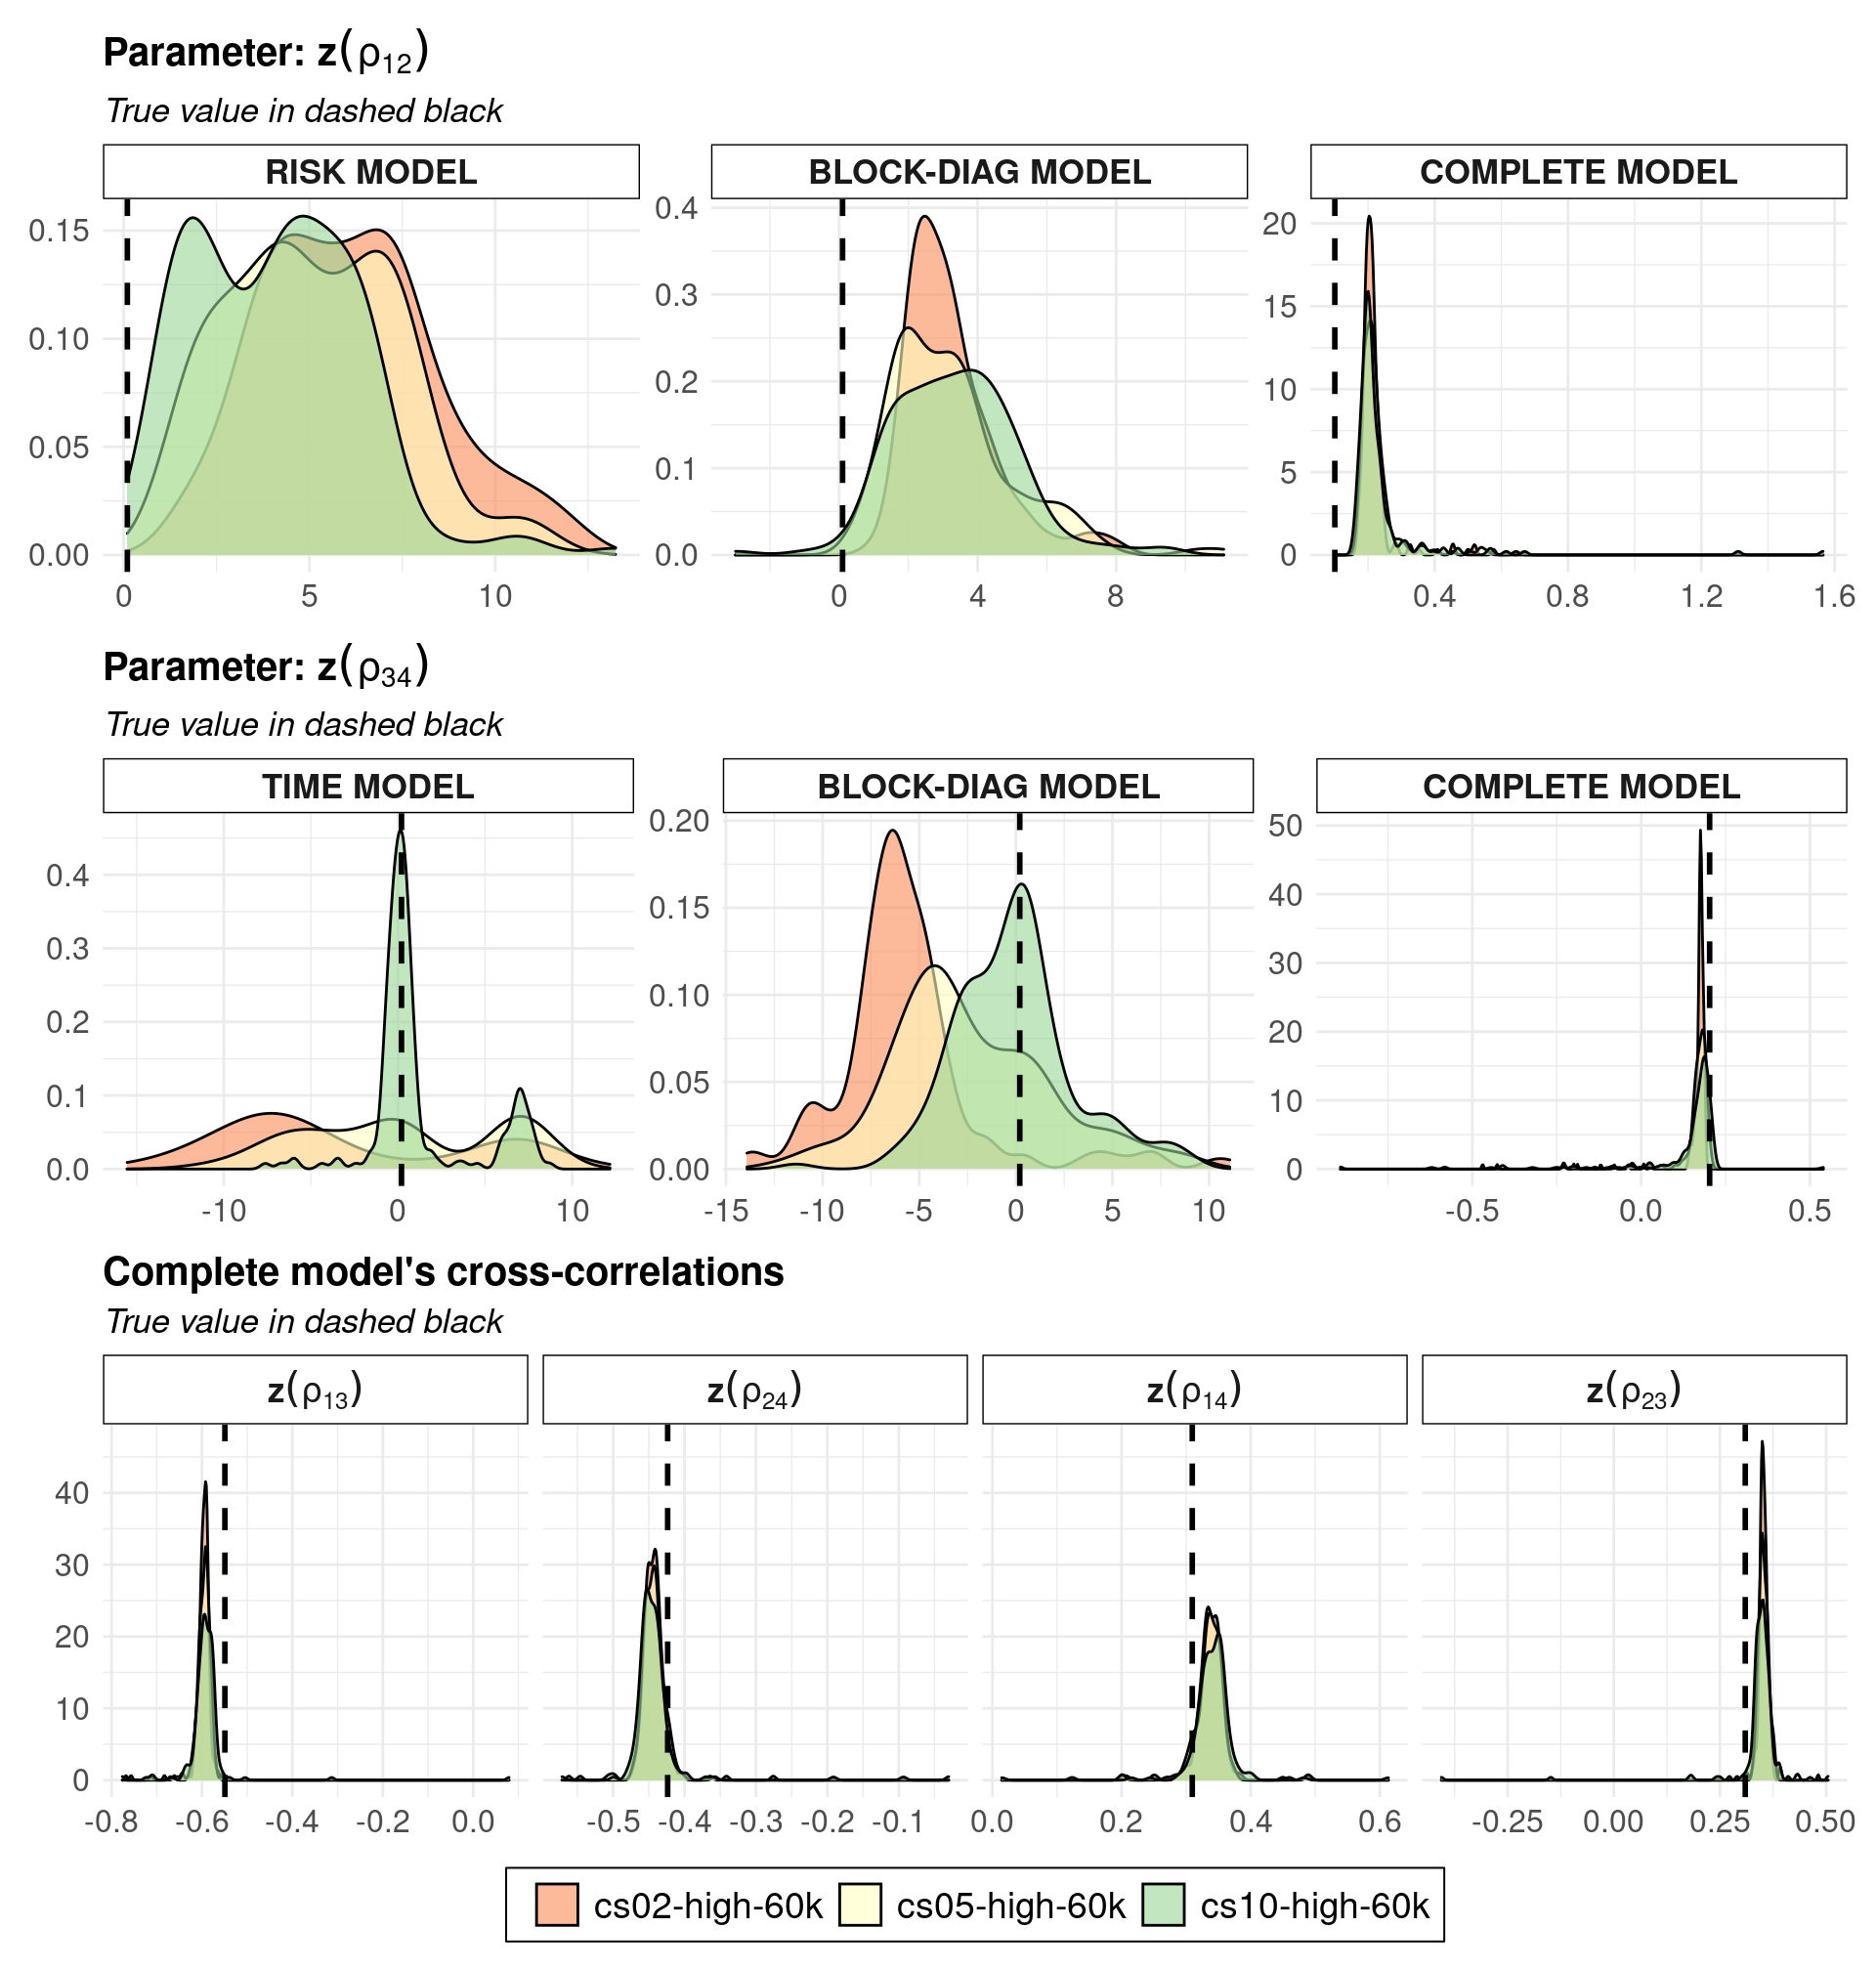
\includegraphics[width=\textwidth]{historhoz-1.png}\\
 \begin{footnotesize}
  SOURCE: The author (2021).
 \end{footnotesize}
 \label{fig:historhoz}
\end{figure}

\begin{figure}[H]
 \setlength{\abovecaptionskip}{.0001pt}
 \caption{COMPLETE MODEL'S PARAMETERS CORRELATION HEAT-MAP IN THE
          SCENARIO OF CLUSTER SIZE 10, HIGH CIF, AND SIXTY-THOUSAND DATA
          POINTS}
 \centering
 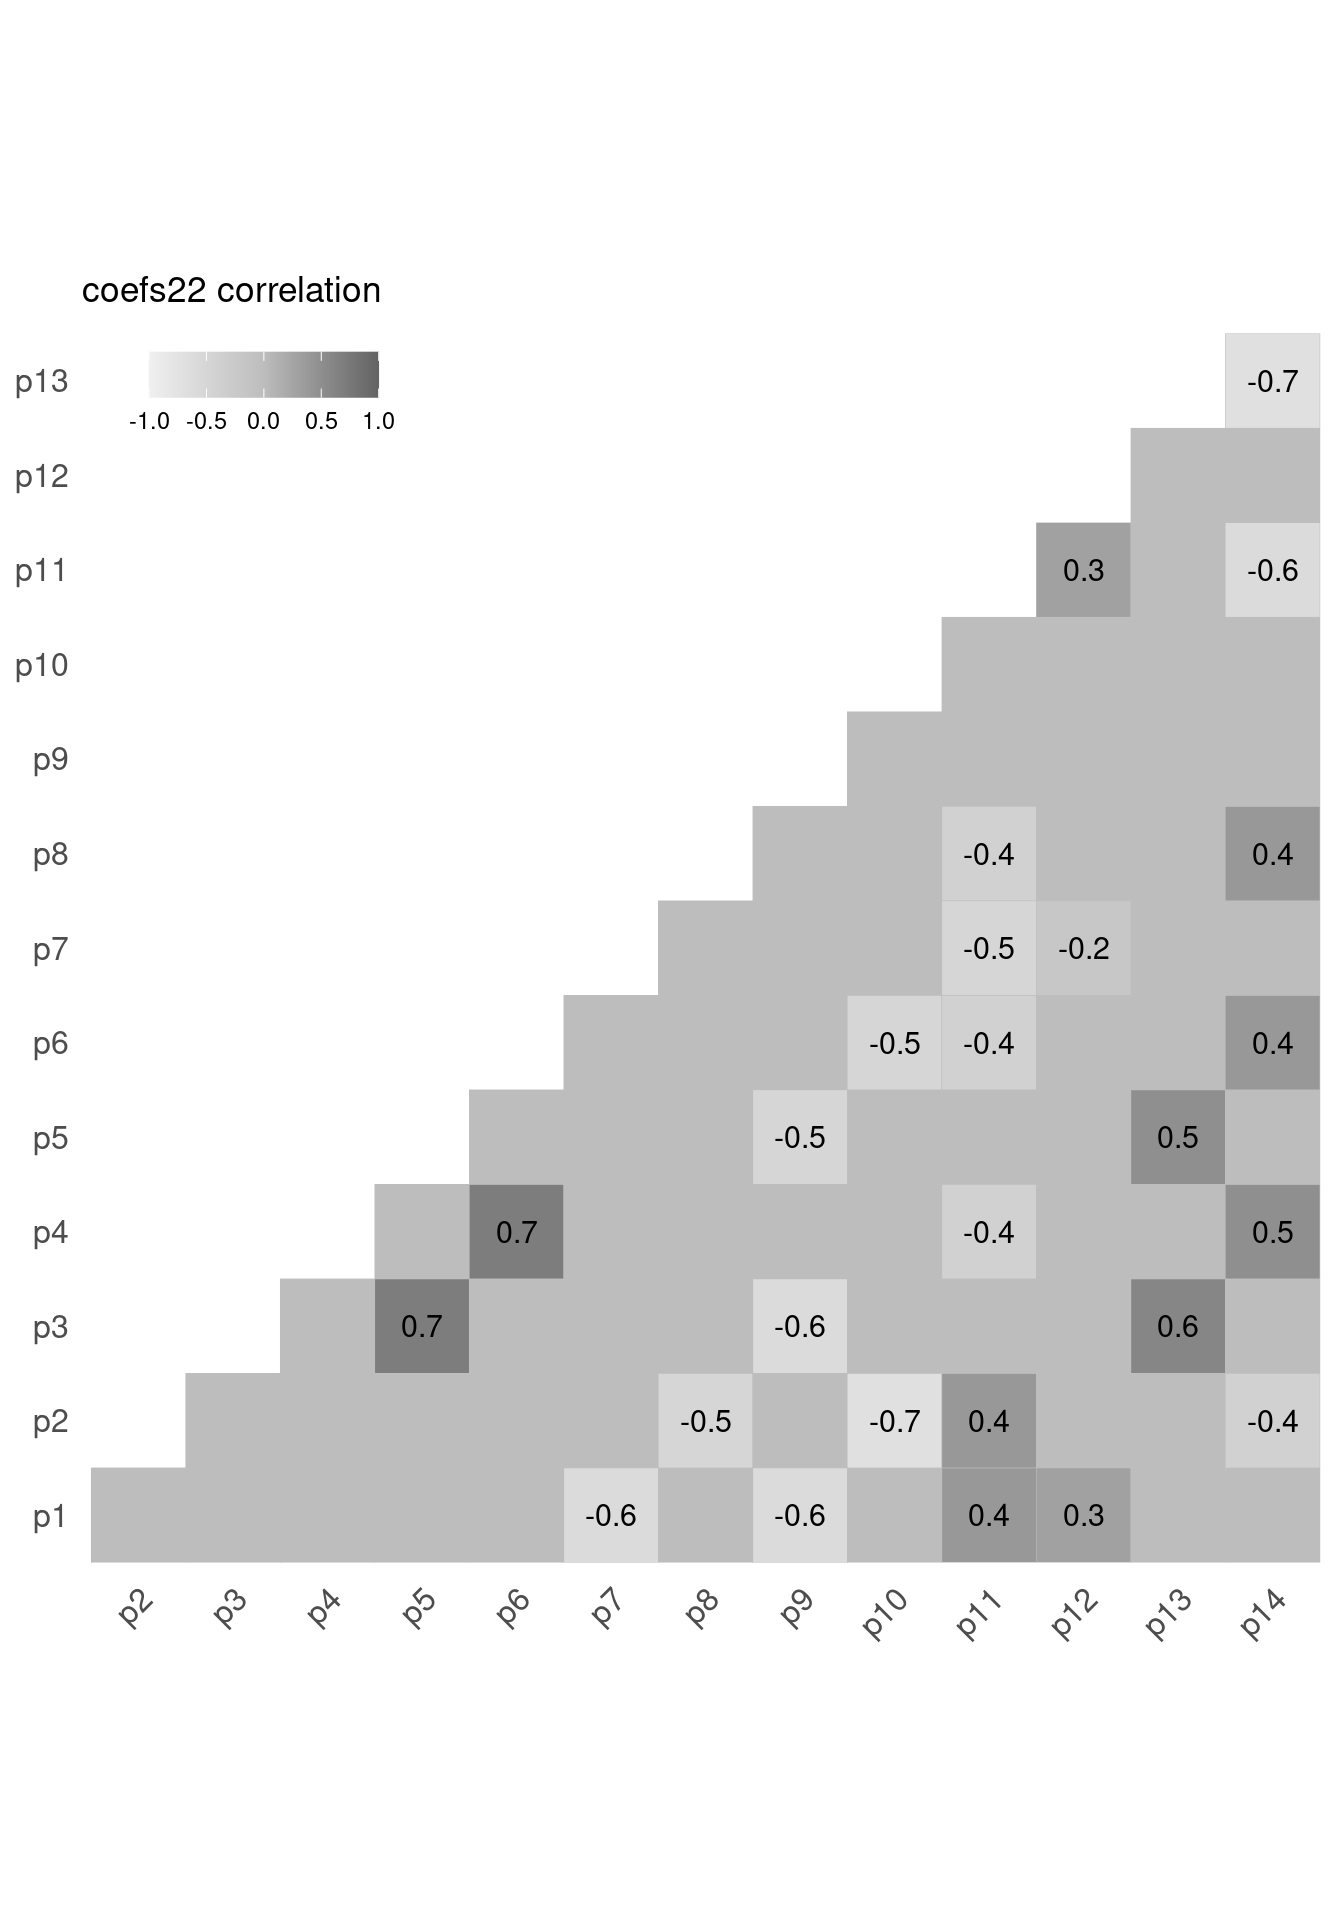
\includegraphics[width=0.85\textwidth]{cor2plot-1.png}\\
 \vspace{-0.2cm}
 \begin{footnotesize}
  SOURCE: The author (2021).
 \end{footnotesize}
 \label{fig:cor2plot}
\end{figure}

% END ==================================================================

% ----------------------------------------------------------------------
\chapter{Final considerations}
\label{cap:finalc}
The general goal of this master thesis was the proposition of a new
regression model for the analysis of clustered competing risks
data. Focused on the modeling of the cumulative incidence function
(CIF), in the probability scale, instead of the hazard scale usual on
the survival modeling literature. We model the clustered competing risks
on a latent-effects framework, a generalized linear mixed model (GLMM)
\cite{GLMM}, with a multinomial distribution for the competing risks and
censorship, conditioned on the possible covariates and
latent-effects. The within-cluster dependency is accommodated by a
multivariate Gaussian distribution and is modeled via its covariance
matrix parameters.

The failures by the competing causes and their respective censorships
are modeled in the probability scale, by means of the CIF
\cite{kalb&prentice, andersen12}. The CIF is accommodated in our GLMM
framework in terms of the link function, as the product of two
functions, one responsible to model the immediate risk and the other the
trajectory time. The shape of these functions is described in detail in
\autoref{cap:model}. This particular GLMM formulation is what makes our
model, particular. Thus, we have what we call a multiGLMM: a multinomial
GLMM for clustered competing risks data.

The two-function product CIF formulation was taken from
\citeonline{SCHEIKE} but there they use a different framework, a
composite likelihood framework \cite{lindsay88, cox&reid04, varin11}.
Here we do a full likelihood analysis instead. A composite approach is
generally used when a full likelihood approach is impossible or
computationally impracticable. Our goal here was to try a full
likelihood framework taking advantage of state-of-art computational
libraries and very efficient algorithm implementations. We have all this
with the \texttt{R} \cite{R21} package TMB \cite{TMB}.

In \autoref{cap:results} our main results are presented, and it is clear
that the multiGLMM works under certain circumstances. The next step was
to compare our results with the ones obtained in \citeonline{SCHEIKE},
with the composite approach. In the GitHub repository
\url{https://github.com/kkholst/mcif/} the authors provide their code.
In \texttt{mcif/inst/examples/datasim.R} they show how to simulate from
the model, and in \texttt{mcif/src/loglik.cpp} they have their marginal
log-likelihood function. We tried to optimize their marginal
log-likelihood over its parameters using basically all \texttt{R}
\texttt{base::optim()} and \texttt{base::nlminb()} available methods, in
the paper was used the BFGS, one of them. We made several scenarios,
using their own simulation scripts and ours, and to our surprise, the
model basically does not work.

The optimization in its majority fails, via any gradient-based algorithm
(BFGS \cite{nocedal&wright}, PORT \cite{PORTreport, PORTpaper},
conjugate gradient (CG) \cite{CG}), generally by Hessian matrix
instability problems, a problem which our multiGLMM also suffers from
when we try to compute the parameters standard errors. When the model
works, it is because we are using the parameter true values as initial
guesses i.e. if the algorithm needs to walk on the log-likelihood
surface following the gradient, it fails. Even when it works, the
estimates are not always good. We also tried with a SANN and a
Nelder-Mead algorithm. SANN \cite{SANN} is a variant of a simulated
annealing method, based on a Metropolis algorithm. Since it is based on
simulation, it takes a lot of time and as the gradient-based methods, do
not work most of the time. The best results were with the Nelder-Mead
\cite{neldermead}, a free-gradient method. Still, it only works when we
use the parameter true values as initial guesses. This situation,
completely the opposite of what is shown in the paper, made impossible
any reasonable comparison between the models. We will enter in contact
with the authors to see what is happening.

All models from the simulation study were run, in a parallelized
fashion, or in a Linux system with
\begin{itemize}
 \item 12 Intel (R) Core (TM) i7-8750H CPU @ 2.20GHz processors,
 \item 16GB RAM,
\end{itemize} 
or in a, also, Linux system with
\begin{itemize}
 \item 30 Intel (R) Xeon (R) CPU E5-2690 v2 @ 3.00GHz processors,
 \item 206GB RAM.
\end{itemize}

The risk and time models are not so time-consuming, generally never
taking more than 5 minutes (at max) to run. The inherent idea is that we
are always performing two-dimension integral approximations and we have
\textit{just} three covariance parameters. With the block-diag model, we
are theoretically in four dimensions. However, since the covariance
matrix is, block-diagonal, we experienced several numerical instability
problems. The solution, as can be seen in the code
in \autoref{cap:blockdiagModel} (\autoref{cap:appendixD}), was to split
it into two two-dimension matrices, since the \(4\times4\) covariance
matrix is block-diagonal. This simple solution solved all numerical
instability problems. The computational time was only a little bit
bigger than with the risk and time models. 

Finally, the complete model. In the biggest scenario, with 60 thousand
data points and clusters of size 2 i.e., 30 thousand four-dimension (ten
parameters in the covariance matrix) integral approximations, the model
fitting takes 30 minutes with TMB, parallelizing it between the
threads. To really understand what we were doing, before doing the TMB
implementation, we did a complete \texttt{R} implementation. We wrote
the marginal log-likelihood based on our own Laplace approximation and
Newton-Raphson implementation (the gradients, \autoref{cap:appendixA},
and Hessian, \autoref{cap:appendixB}, were computed by hand and
implemented). Running this complete \texttt{R} implementation in a
scenario with 20 thousand data points and clusters of size 2, took
around 30 hours, parallelizing it between all threads of the first Linux
system described above. In summary, we increase the model size 3 times
and the computational time decreased 60 times. The performance gain by
using TMB was incredible.

Still, with the complete model, we performed a Bayesian analysis via
\texttt{tmbstan}.

\section{FUTURE WORKS}
\label{cap:future}

% END ==================================================================

% ----------------------------------------------------------------------
\setlength{\afterchapskip}{\baselineskip}
% ----------------------------------------------------------------------
\bibliography{references}
% ----------------------------------------------------------------------
\postextual
% ----------------------------------------------------------------------
\begin{apendicesenv}
\partapendices
\addcontentsline{toc}{chapter}{\hspace{2.105cm}APPENDIX}
\renewcommand{\ABNTEXchapterfontsize}{\ABNTEXsectionfont}

\chapter{ANALYTIC GRADIENT OF THE LATENT EFFECTS FOR THE JOINT
         LOG-LIKELIHOOD FUNCTION OF THE MULTINOMIAL GLMM FOR CLUSTERED
         COMPETING RISKS DATA}
\label{cap:appendixA}

The following gradient components are computed by cluster, to be used
e.g., in a Newton optimization. Subject \(i\) at cluster \(j\) and for
competing cause \(k\)

\begin{align*}
  &\frac{\partial}{\partial u_{kj}}
    \log L(\bm{\theta}\mid\bm{y}_{j}, \bm{r}_{j}) =\\
  &y_{kij}\frac{1 +
    \sum_{m \neq k}^{K-1}\exp\{\bm{x}_{mij}\bm{\beta}_{mj} + u_{mj}\}
    }{1 +
    \sum_{n = 1}^{K-1}\exp\{\bm{x}_{nij}\bm{\beta}_{nj} + u_{nj}\}} -
    \left(\sum_{m \neq k}^{K-1} y_{mij}\right)
    \frac{\exp\{\bm{x}_{kij}\bm{\beta}_{kj} + u_{kj}\}
    }{1 +
    \sum_{n = 1}^{K-1}\exp\{\bm{x}_{nij}\bm{\beta}_{nj} + u_{nj}\}}-\\
  &y_{Kij}\frac{1}{1 +
    \sum_{n = 1}^{K-1}\exp\{\bm{x}_{nij}\bm{\beta}_{nj} + u_{nj}\}
    }\Bigg(\\
  &\frac{\exp\{\bm{x}_{kij}\bm{\beta}_{kj} + u_{kj}\}
    \left(1 +
    \sum_{m \neq k}^{K-1}\exp\{\bm{x}_{mij}\bm{\beta}_{mj} + u_{mj}\}
    \right)}{
    1 + \sum_{n = 1}^{K-1}\exp\{\bm{x}_{nij}\bm{\beta}_{nj} + u_{nj}\}
    }\times\\
  &\frac{w_{k}\frac{\delta}{2\delta t - 2t^{2}}
    \phi[w_{k}\text{arctanh}\left(\frac{t-\delta/2}{\delta/2}\right)
    - \bm{x}_{kij}\bm{\gamma}_{kj} - \eta_{kj}
    ]}{1 - w_{n}\frac{\delta}{2\delta t - 2t^{2}}
    \phi[w_{n}\text{arctanh}\left(\frac{t-\delta/2}{\delta/2}\right)
    - \bm{x}_{nij}\bm{\gamma}_{nj} - \eta_{nj}]} -
    \frac{\exp\{\bm{x}_{kij}\bm{\beta}_{kj} + u_{kj}\}}{
    1 + \sum_{n = 1}^{K-1}\exp\{\bm{x}_{nij}\bm{\beta}_{nj} + u_{nj}\}}
    \times\\
  &\frac{
    \sum_{m \neq k}^{K-1}
    w_{m}\frac{\delta}{2\delta t - 2t^{2}}
    \phi[w_{m}\text{arctanh}\left(\frac{t-\delta/2}{\delta/2}\right)
    - \bm{x}_{mij}\bm{\gamma}_{mj} - \eta_{mj}]
    \exp\{\bm{x}_{mij}\bm{\beta}_{mj} + u_{mj}\}}{
    1 - w_{n}\frac{\delta}{2\delta t - 2t^{2}}
    \phi[w_{n}\text{arctanh}\left(\frac{t-\delta/2}{\delta/2}\right)
    - \bm{x}_{nij}\bm{\gamma}_{nj} - \eta_{nj}]}\Bigg) -\\
  &\bm{e_{k}^{\top}Qr_{j}},\\
  %% -------------------------------------------------------------------
  \\
  %% -------------------------------------------------------------------
  &\frac{\partial}{\partial \eta_{kj}}
  \log L(\bm{\theta}\mid\bm{y}_{j}, \bm{r}_{j}) =\\
  &y_{kij} (w_{k}\text{arctanh}\left(\frac{t-\delta/2}{\delta/2}\right)
    - \bm{x}_{kij}\bm{\gamma}_{kj} - \eta_{kj}) -\\
  &y_{Kij}\frac{\exp\{\bm{x}_{kij}\bm{\beta}_{kj} + u_{kj}\}
    }{1 + \sum_{n = 1}^{K-1}\exp\{\bm{x}_{nij}\bm{\beta}_{nj} + u_{nj}\}}
    \times\\
  &\frac{
    w_{k}\frac{\delta}{2\delta t - 2t^{2}}
    (w_{k}\text{arctanh}\left(\frac{t-\delta/2}{\delta/2}\right)
    - \bm{x}_{kij}\bm{\gamma}_{kj} - \eta_{kj})
    \phi[w_{k} \text{arctanh}\left(\frac{t-\delta/2}{\delta/2}\right)
    - \bm{x}_{kij}\bm{\gamma}_{kj} - \eta_{kj}
    ]}{1 -
    \sum_{n = 1}^{K-1}
    \frac{\exp\{\bm{x}_{nij}\bm{\beta}_{nj} + u_{nj}\}}{1 +
    \sum_{n = 1}^{K-1}\exp\{\bm{x}_{nij}\bm{\beta}_{nj} + u_{nj}\}}
    w_{n}\frac{\delta}{2\delta t - 2t^{2}}
    \phi[w_{n}\text{arctanh}\left(\frac{t-\delta/2}{\delta/2}\right)
    - \bm{x}_{nij}\bm{\gamma}_{nj} - \eta_{nj}]} -\\
  &\bm{e_{k}^{\top}Qr_{j}},
\end{align*}
with \(\bm{e_{k}^{\top}}\) begin a vector with \(1\) at the \(k\)-th
position and zero elsewhere.

\chapter{ANALYTIC HESSIAN OF THE LATENT EFFECTS FOR THE JOINT
         LOG-LIKELIHOOD FUNCTION OF THE MULTINOMIAL GLMM FOR CLUSTERED
         COMPETING RISKS DATA}
\label{cap:appendixB}

The following hessian components are computed by cluster, to be used
e.g., in a Newton optimization. Subject \(i\) at cluster \(j\) and for
competing cause \(k\)
\begin{align*}
  &\frac{\partial^{2}}{\partial u_{kj}^{2}}
    \log L(\bm{\theta}\mid\bm{y}_{j}, \bm{r}_{j}) =\\
  &-\frac{\left(\sum_{k = 1}^{K-1} y_{kij}\right)
    \exp\{\bm{x}_{kij}\bm{\beta}_{kj} + u_{kj}\}
    \left(1 +
    \sum_{m \neq k}^{K-1}\exp\{\bm{x}_{mij}\bm{\beta}_{mj} + u_{mj}\}
    \right)}{\left(1 +
    \sum_{n = 1}^{K-1}\exp\{\bm{x}_{nij}\bm{\beta}_{nj} + u_{nj}\}
    \right)^{2}} +\\
  &\frac{y_{Kij}
    \exp\{\bm{x}_{kij} \bm{\beta}_{kj} + u_{kj}\}}{
    1 + \sum_{n = 1}^{K-1}\exp\{\bm{x}_{nij} \bm{\beta}_{nj} + u_{nj}\}
    }\times\\
  &\frac{
    \sum_{m \neq k}^{K-1}w_{m}\frac{\delta}{2\delta t - 2t^{2}}
    \phi[w_{m}\text{arctanh}\left(\frac{t-\delta/2}{\delta/2}\right)
    - \bm{x}_{mij}\bm{\gamma}_{mj} - \eta_{mj}]
    \exp\{\bm{x}_{mij}\bm{\beta}_{mj} + u_{mj}\}}{1 +
    \sum_{n = 1}^{K-1}\exp\{\bm{x}_{nij}\bm{\beta}_{nj} + u_{nj}\}
    (1 - w_{n}\frac{\delta}{2\delta t - 2t^{2}}
    \phi[w_{n}\text{arctanh}\left(\frac{t-\delta/2}{\delta/2}\right)
    - \bm{x}_{nij}\bm{\gamma}_{nj} - \eta_{nj}])} -\\
  &\frac{
    y_{Kij}
    w_{k}\frac{\delta}{2\delta t - 2t^{2}}
    \phi[w_{k}\text{arctanh}\left(\frac{t-\delta/2}{\delta/2}\right)
    - \bm{x}_{kij}\bm{\gamma}_{kj} - \eta_{kj}] }{1 +
    \sum_{n = 1}^{K-1}\exp\{\bm{x}_{nij}\bm{\beta}_{nj} + u_{nj}\}
    }\times\\
  &\frac{\exp\{\bm{x}_{kij}\bm{\beta}_{kj} + u_{kj}\}
    \left(1 +
    \sum_{m \neq k}^{K-1}\exp\{\bm{x}_{mij}\bm{\beta}_{mj} + u_{mj}\}
    \right)}{1 +
    \sum_{n = 1}^{K-1}\exp\{\bm{x}_{nij}\bm{\beta}_{nj} + u_{nj}\}
    (1 - w_{n}\frac{\delta}{2\delta t - 2t^{2}}
    \phi[w_{n}\text{arctanh}\left(\frac{t-\delta/2}{\delta/2}\right)
    - \bm{x}_{nij}\bm{\gamma}_{nj} - \eta_{nj}])} -\\
  &\frac{y_{Kij}\exp\{\bm{x}_{kij}\bm{\beta}_{kj} + u_{kj}\}}{\left(1 +
    \sum_{n = 1}^{K-1}\exp\{\bm{x}_{nij}\bm{\beta}_{nj} + u_{nj}\}
    \right)^{2}}\Bigg(\\
  &\frac{\sum_{m \neq k}^{K-1}
    w_{m}\frac{\delta}{2\delta t - 2t^{2}}
    \phi[w_{m}\text{arctanh}\left(\frac{t-\delta/2}{\delta/2}\right)
    - \bm{x}_{mij}\bm{\gamma}_{mj} - \eta_{mj}]
    \exp\{\bm{x}_{mij}\bm{\beta}_{mj} + u_{mj}\}}{\left(1 +
    \sum_{n = 1}^{K-1}\exp\{\bm{x}_{nij}\bm{\beta}_{nj} + u_{nj}\}
    (1 - w_{n}\frac{\delta}{2\delta t - 2t^{2}}
    \phi[w_{n}\text{arctanh}\left(\frac{t-\delta/2}{\delta/2}\right)
    - \bm{x}_{nij}\bm{\gamma}_{nj} - \eta_{nj}])\right)^{2}}-\\
  &\frac{w_{k}\frac{\delta}{2\delta t - 2t^{2}}
    \phi[w_{k}\text{arctanh}\left(\frac{t-\delta/2}{\delta/2}\right)
    - \bm{x}_{kij}\bm{\gamma}_{kj} - \eta_{kj}]\left(1 +
    \sum_{m \neq k}^{K-1}\exp\{\bm{x}_{mij}\bm{\beta}_{mj} + u_{mj}\}
    \right)}{\left(1 +
    \sum_{n = 1}^{K-1}\exp\{\bm{x}_{nij}\bm{\beta}_{nj} + u_{nj}\}
    (1 - w_{n}\frac{\delta}{2\delta t - 2t^{2}}
    \phi[w_{n}\text{arctanh}\left(\frac{t-\delta/2}{\delta/2}\right)
    - \bm{x}_{nij}\bm{\gamma}_{nj} - \eta_{nj}])\right)^{2}}\Bigg)\\
  &\times\Bigg(\Big(1 +\\
  &\sum_{n = 1}^{K-1}\exp\{\bm{x}_{nij}\bm{\beta}_{nj} + u_{nj}\}
    (1 - w_{n}\frac{\delta}{2\delta t - 2t^{2}}
    \phi[w_{n}\text{arctanh}\left(\frac{t-\delta/2}{\delta/2}\right)
    - \bm{x}_{nij}\bm{\gamma}_{nj} - \eta_{nj}])\Big) +\\
  &\Big(1 +
    \sum_{n = 1}^{K-1}\exp\{\bm{x}_{nij} \bm{\beta}_{nj} + u_{nj}\}
    \Big)\times\\
  &(1 - w_{k}\frac{\delta}{2\delta t - 2t^{2}}
    \phi[w_{k}\text{arctanh}\left(\frac{t-\delta/2}{\delta/2}\right)
    - \bm{x}_{kij}\bm{\gamma}_{kj} - \eta_{kj}])\Bigg)
    - \bm{e_{k}^{\top}Q},
\end{align*}

\begin{align*}
  &\frac{\partial^{2}}{\partial \eta_{kj}^{2}}
    \log L(\bm{\theta}\mid\bm{y}_{j}, \bm{r}_{j}) =\\
  &- y_{kij} - y_{Kij}
    \frac{\exp\{\bm{x}_{kij} \bm{\beta}_{kj} + u_{kj}\}}{1 +
    \sum_{n = 1}^{K-1}\exp\{\bm{x}_{nij} \bm{\beta}_{nj} + u_{nj}\}}\Bigg(\\
  &w_{k}\frac{\delta}{2\delta t - 2t^{2}}
    \phi[w_{k}\text{arctanh}\left(\frac{t-\delta/2}{\delta/2}\right)
    - \bm{x}_{kij}\bm{\gamma}_{kj} - \eta_{kj}]\times\\
  &\frac{\left(
    w_{k} \text{arctanh}\left(\frac{t-\delta/2}{\delta/2}\right)
    - \bm{x}_{kij}\bm{\gamma}_{kj} - \eta_{kj}
    \right)^{2} - 1}{
    1 - \sum_{n = 1}^{K-1}
    \frac{\exp\{\bm{x}_{nij}\bm{\beta}_{nj} + u_{nj}\}}{1 +
    \sum_{n = 1}^{K-1}\exp\{\bm{x}_{nij} \bm{\beta}_{nj} + u_{nj}\}}
    w_{n}\frac{\delta}{2\delta t - 2t^{2}}
    \phi[w_{n}\text{arctanh}\left(\frac{t-\delta/2}{\delta/2}\right)
    - \bm{x}_{nij}\bm{\gamma}_{nj} - \eta_{nj}]} -\\
  &\frac{\left(
    w_{k}\frac{\delta}{2\delta t - 2t^{2}}
    (w_{k}\text{arctanh}\left(\frac{t-\delta/2}{\delta/2}\right)
    - \bm{x}_{kij}\bm{\gamma}_{kj} - \eta_{kj})
    \phi[w_{k}\text{arctanh}\left(\frac{t-\delta/2}{\delta/2}\right)
    - \bm{x}_{kij}\bm{\gamma}_{kj} - \eta_{kj}]\right)^{2}}{\left(1 -
    \sum_{n = 1}^{K-1}
    \frac{\exp\{\bm{x}_{nij} \bm{\beta}_{nj} + u_{nj}\}}{1 +
    \sum_{n = 1}^{K-1}\exp\{\bm{x}_{nij} \bm{\beta}_{nj} + u_{nj}\}}
    w_{n}\frac{\delta}{2\delta t - 2t^{2}}
    \phi[w_{n}\text{arctanh}\left(\frac{t-\delta/2}{\delta/2}\right)
    - \bm{x}_{nij}\bm{\gamma}_{nj} - \eta_{nj}]\right)^{2}}\\
  &\Bigg) - \bm{e_{k}^{\top}Q},
\end{align*}

\begin{align*}
  &\frac{\partial^{2}}{\partial u_{kj} u_{mj}}
    \log L(\bm{\theta}\mid\bm{y}_{j}, \bm{r}_{j}) =\\
  &\left(\sum_{k = 1}^{K-1} y_{kij}\right)
    \frac{
    \exp\{\bm{x}_{kij}\bm{\beta}_{kj} + u_{kj}\}
    \exp\{\bm{x}_{mij}\bm{\beta}_{mj} + u_{mj}\}}{
    \left(1 +
    \sum_{n = 1}^{K-1}\exp\{\bm{x}_{nij} \bm{\beta}_{nj} + u_{nj}\}
    \right)^{2}} +\\
  &\frac{
    y_{Kij}
    \exp\{\bm{x}_{kij}\bm{\beta}_{kj} + u_{kj}\}
    \exp\{\bm{x}_{mij} \bm{\beta}_{mj} + u_{mj}\}}{1 +
    \sum_{n = 1}^{K-1}\exp\{\bm{x}_{nij} \bm{\beta}_{nj} + u_{nj}\}}\Bigg(\\
  &\frac{
    w_{m}\frac{\delta}{2\delta t - 2t^{2}}
    \phi[w_{m}\text{arctanh}\left(\frac{t-\delta/2}{\delta/2}\right)
    - \bm{x}_{mij}\bm{\gamma}_{mj} - \eta_{mj}]}{1 +
    \sum_{n = 1}^{K-1}\exp\{\bm{x}_{nij} \bm{\beta}_{nj} + u_{nj}\}
    (1 - w_{n}\frac{\delta}{2\delta t - 2t^{2}}
    \phi[w_{n}\text{arctanh}\left(\frac{t-\delta/2}{\delta/2}\right)
    - \bm{x}_{nij}\bm{\gamma}_{nj} - \eta_{nj}])} -\\
  &\frac{
    w_{k}\frac{\delta}{2\delta t - 2t^{2}}
    \phi[w_{k}\text{arctanh}\left(\frac{t-\delta/2}{\delta/2}\right)
    - \bm{x}_{kij}\bm{\gamma}_{kj} - \eta_{kj}]}{1 +
    \sum_{n = 1}^{K-1}\exp\{\bm{x}_{nij}\bm{\beta}_{nj} + u_{nj}\}
    (1 - w_{n}\frac{\delta}{2\delta t - 2t^{2}}
    \phi[w_{n}\text{arctanh}\left(\frac{t-\delta/2}{\delta/2}\right)
    - \bm{x}_{nij}\bm{\gamma}_{nj} - \eta_{nj}])}\Bigg) -\\
  &\frac{y_{Kij}}{
    \left(1 +
    \sum_{n = 1}^{K-1}\exp\{\bm{x}_{nij}\bm{\beta}_{nj} + u_{nj}\}
    \right)^{2}}\Bigg(\exp\{\bm{x}_{kij}\bm{\beta}_{kj} + u_{kj}\}\Bigg(\\
  &\frac{
    \sum_{m \neq k}^{K-1}
    w_{m}\frac{\delta}{2\delta t - 2t^{2}}
    \phi[w_{m}\text{arctanh}\left(\frac{t-\delta/2}{\delta/2}\right)
    - \bm{x}_{mij}\bm{\gamma}_{mj} - \eta_{mj}]
    \exp\{\bm{x}_{mij} \bm{\beta}_{mj} + u_{mj}\}}{
    \left(1 + \sum_{n = 1}^{K-1}\exp\{\bm{x}_{nij}\bm{\beta}_{nj} + u_{nj}\}
    (1 - w_{n}\frac{\delta}{2\delta t - 2t^{2}}
    \phi[w_{n}\text{arctanh}\left(\frac{t-\delta/2}{\delta/2}\right)
    - \bm{x}_{nij}\bm{\gamma}_{nj} - \eta_{nj}])\right)^{2}} -\\
  &\frac{
    w_{k}\frac{\delta}{2\delta t - 2t^{2}}
    \phi[w_{k}\text{arctanh}\left(\frac{t-\delta/2}{\delta/2}\right)
    - \bm{x}_{kij}\bm{\gamma}_{kj} - \eta_{kj}]
    \left(1 +
    \sum_{m \neq k}^{K-1}\exp\{\bm{x}_{mij}\bm{\beta}_{mj} + u_{mj}\}
    \right)}{\left(1 +
    \sum_{n = 1}^{K-1}\exp\{\bm{x}_{nij} \bm{\beta}_{nj} + u_{nj}\}
    (1 - w_{n}\frac{\delta}{2\delta t - 2t^{2}}
    \phi[w_{n}\text{arctanh}\left(\frac{t-\delta/2}{\delta/2}\right)
    - \bm{x}_{nij}\bm{\gamma}_{nj} - \eta_{nj}])\right)^{2}}\Bigg)
\end{align*}
\begin{align*}
  &\Bigg)\times\Bigg(\exp\{\bm{x}_{mij}\bm{\beta}_{mj} + u_{mj}\}
    \Big(1 +\\
  &\sum_{n = 1}^{K-1}\exp\{\bm{x}_{nij}\bm{\beta}_{nj} + u_{nj}\}
    (1 - w_{n}\frac{\delta}{2\delta t - 2t^{2}}
    \phi[w_{n}\text{arctanh}\left(\frac{t-\delta/2}{\delta/2}\right)
    - \bm{x}_{nij}\bm{\gamma}_{nj} - \eta_{nj}])\Big) +\\
  &\exp\{\bm{x}_{mij}\bm{\beta}_{mj} + u_{mj}\}
    (1 - w_{m}\frac{\delta}{2\delta t - 2t^{2}}
    \phi[w_{m}\text{arctanh}\left(\frac{t-\delta/2}{\delta/2}\right)
    - \bm{x}_{mij}\bm{\gamma}_{mj} - \eta_{mj}])\Big(1 +\\
  &\sum_{n = 1}^{K-1}\exp\{\bm{x}_{nij}\bm{\beta}_{nj} + u_{nj}\}\Big)
    \Bigg) - \bm{e_{k}^{\top}Q},
\end{align*}

\begin{align*}
  &\frac{\partial^{2}}{\partial \eta_{kj} \eta_{mj}}
    \log L(\bm{\theta}\mid\bm{y}_{j}, \bm{r}_{j}) =\\
  &- y_{Kij}\frac{
    \exp\{\bm{x}_{kij}\bm{\beta}_{kj} + u_{kj}\}}{1 +
    \sum_{n = 1}^{K-1}\exp\{\bm{x}_{nij}\bm{\beta}_{nj} + u_{nj}\}}\times\\
  &\frac{w_{k}\frac{\delta}{2\delta t - 2t^{2}}
    (w_{k}\text{arctanh}\left(\frac{t-\delta/2}{\delta/2}\right)
    - \bm{x}_{kij}\bm{\gamma}_{kj} - \eta_{kj})
    \phi[w_{k}\text{arctanh}\left(\frac{t-\delta/2}{\delta/2}\right)
    - \bm{x}_{kij}\bm{\gamma}_{kj} - \eta_{kj}]}{\left(1 -
    \sum_{n = 1}^{K-1}\frac{\exp\{\bm{x}_{nij}\bm{\beta}_{nj} + u_{nj}\}
    }{1 +
    \sum_{n = 1}^{K-1}\exp\{\bm{x}_{nij}\bm{\beta}_{nj} + u_{nj}\}}
    w_{n}\frac{\delta}{2\delta t - 2t^{2}}
    \phi[w_{n}\text{arctanh}\left(\frac{t-\delta/2}{\delta/2}\right)
    - \bm{x}_{nij}\bm{\gamma}_{nj} - \eta_{nj}]\right)^{2}}\times\\
  &\frac{\exp\{\bm{x}_{mij}\bm{\beta}_{mj} + u_{mj}\}}{1 +
    \sum_{n = 1}^{K-1}\exp\{\bm{x}_{nij}\bm{\beta}_{nj} + u_{nj}\}}
    w_{m}\frac{\delta}{2\delta t - 2t^{2}}
    (w_{m}\text{arctanh}\left(\frac{t-\delta/2}{\delta/2}\right)
    - \bm{x}_{mij}\bm{\gamma}_{mj} - \eta_{mj})\times\\
  &\phi[w_{m}\text{arctanh}\left(\frac{t-\delta/2}{\delta/2}\right)
    - \bm{x}_{mij}\bm{\gamma}_{mj} - \eta_{mj}] - \bm{e_{k}^{\top}Q},
\end{align*}

\begin{align*}
  &\frac{\partial^{2}}{\partial \eta_{kj} u_{kj}}
    \log L(\bm{\theta}\mid\bm{y}_{j}, \bm{r}_{j}) =\\
  &y_{Kij}
    \frac{\exp\{\bm{x}_{kij}\bm{\beta}_{kj} + u_{kj}\}}{1 +
    \sum_{n = 1}^{K-1}\exp\{\bm{x}_{nij}\bm{\beta}_{nj} + u_{nj}\}}\times\\
  &\frac{
    w_{k}\frac{\delta}{2\delta t - 2t^{2}}
    (w_{k}\text{arctanh}\left(\frac{t-\delta/2}{\delta/2}\right)
    - \bm{x}_{kij}\bm{\gamma}_{kj} - \eta_{kj})
    \phi[w_{k}\text{arctanh}\left(\frac{t-\delta/2}{\delta/2}\right)
    - \bm{x}_{kij}\bm{\gamma}_{kj} - \eta_{kj})]}{
    \left(1 -
    \sum_{n = 1}^{K-1}\frac{\exp\{\bm{x}_{nij}\bm{\beta}_{nj} + u_{nj}\}}{
    1 +
    \sum_{n = 1}^{K-1}\exp\{\bm{x}_{nij}\bm{\beta}_{nj} + u_{nj}\}}
    w_{n}\frac{\delta}{2\delta t - 2t^{2}}
    \phi[w_{n}\text{arctanh}\left(\frac{t-\delta/2}{\delta/2}\right)
    - \bm{x}_{nij}\bm{\gamma}_{nj} - \eta_{nj}]\right)^{2}}\times\\
  &\Bigg(
    \sum_{n \neq k}^{K-1}
    \frac{
    \exp\{\bm{x}_{nij}\bm{\beta}_{nj} + u_{nj}\}
    \exp\{\bm{x}_{kij}\bm{\beta}_{kj} + u_{kj}\}}{
    \left(1 +
    \sum_{n = 1}^{K-1}\exp\{\bm{x}_{nij}\bm{\beta}_{nj} + u_{nj}\}
    \right)^{2}}\times\\
  &w_{n}\frac{\delta}{2\delta t - 2t^{2}}
    \phi[w_{n}\text{arctanh}\left(\frac{t-\delta/2}{\delta/2}\right)
    - \bm{x}_{nij}\bm{\gamma}_{nj} - \eta_{nj}] -\\
  &\frac{\exp\{\bm{x}_{kij}\bm{\beta}_{kj} + u_{kj}\}
    \left(
    \left(1 +
    \sum_{n = 1}^{K-1}\exp\{\bm{x}_{nij}\bm{\beta}_{nj} + u_{nj}\}
    \right) - \exp\{\bm{x}_{kij} \bm{\beta}_{kj} + u_{kj}\}
    \right)}{
    \left(1 +
    \sum_{n = 1}^{K-1}\exp\{\bm{x}_{nij}\bm{\beta}_{nj} + u_{nj}\}
    \right)^{2}}\times\\
  &w_{k}\frac{\delta}{2\delta t - 2t^{2}}
    \phi[w_{k}\text{arctanh}\left(\frac{t-\delta/2}{\delta/2}\right)
    - \bm{x}_{kij}\bm{\gamma}_{kj} - \eta_{kj}]\Bigg) -
\end{align*}
\begin{align*}
  &y_{Kij}
    \frac{
    \frac{\exp\{\bm{x}_{kij}\bm{\beta}_{kj} + u_{kj}\}
    \left(
    \left(1 +
    \sum_{n = 1}^{K-1}\exp\{\bm{x}_{nij}\bm{\beta}_{nj} + u_{nj}\}
    \right) - \exp\{\bm{x}_{kij} \bm{\beta}_{kj} + u_{kj}\}
    \right)}{
    \left(1 +
    \sum_{n = 1}^{K-1}\exp\{\bm{x}_{nij}\bm{\beta}_{nj} + u_{nj}\}
    \right)^{2}}}{1 -
    \sum_{n = 1}^{K-1}\frac{\exp\{\bm{x}_{nij}\bm{\beta}_{nj} + u_{nj}\}}{
    1 + \sum_{n = 1}^{K-1}\exp\{\bm{x}_{nij}\bm{\beta}_{nj} + u_{nj}\}}
    w_{n}\frac{\delta}{2\delta t - 2t^{2}}
    \phi[w_{n}\text{arctanh}\left(\frac{t-\delta/2}{\delta/2}\right)
    - \bm{x}_{nij}\bm{\gamma}_{nj} - \eta_{nj}]}\times\\
  &w_{k}\frac{\delta}{2\delta t - 2t^{2}}
    (w_{k}\text{arctanh}\left(\frac{t-\delta/2}{\delta/2}\right)
    - \bm{x}_{kij}\bm{\gamma}_{kj} - \eta_{kj})\times\\
  &\phi[w_{k}\text{arctanh}\left(\frac{t-\delta/2}{\delta/2}\right)
    - \bm{x}_{kij}\bm{\gamma}_{kj} - \eta_{kj}] - \bm{e_{k}^{\top}Q},
\end{align*}

\begin{align*}
  &\frac{\partial^{2}}{\partial \eta_{kj} u_{mj}}
    \log L(\bm{\theta}\mid\bm{y}_{j}, \bm{r}_{j}) =\\
  &y_{Kij}
    \frac{\exp\{\bm{x}_{kij}\bm{\beta}_{kj} + u_{kj}\}
    \exp\{\bm{x}_{mij}\bm{\beta}_{mj} + u_{mj}\}}{
    \left(1 +
    \sum_{n = 1}^{K-1}\exp\{\bm{x}_{nij}\bm{\beta}_{nj} + u_{nj}\}
    \right)^{2}}\times\\
  &\frac{
    w_{k}\frac{\delta}{2\delta t - 2t^{2}}
    (w_{k} \text{arctanh}\left(\frac{t-\delta/2}{\delta/2}\right)
    - \bm{x}_{kij}\bm{\gamma}_{kj} - \eta_{kj})
    \phi[w_{k}\text{arctanh}\left(\frac{t-\delta/2}{\delta/2}\right)
    - \bm{x}_{kij}\bm{\gamma}_{kj} - \eta_{kj})]}{1 - \sum_{n = 1}^{K-1}
    \frac{\exp\{\bm{x}_{nij}\bm{\beta}_{nj} + u_{nj}\}}{1 +
    \sum_{n = 1}^{K-1}\exp\{\bm{x}_{nij}\bm{\beta}_{nj} + u_{nj}\}}
    w_{n}\frac{\delta}{2\delta t - 2t^{2}}
    \phi[w_{n}\text{arctanh}\left(\frac{t-\delta/2}{\delta/2}\right)
    - \bm{x}_{nij}\bm{\gamma}_{nj} - \eta_{nj}]} +\\
  &y_{Kij}
    \frac{\exp\{\bm{x}_{kij}\bm{\beta}_{kj} + u_{kj}\}}{1 +
    \sum_{n = 1}^{K-1}\exp\{\bm{x}_{nij}\bm{\beta}_{nj} + u_{nj}\}}\times\\
  &\frac{
    w_{k}\frac{\delta}{2\delta t - 2t^{2}}
    (w_{k}\text{arctanh}\left(\frac{t-\delta/2}{\delta/2}\right)
    - \bm{x}_{kij}\bm{\gamma}_{kj} - \eta_{kj})
    \phi[w_{k}\text{arctanh}\left(\frac{t-\delta/2}{\delta/2}\right)
    - \bm{x}_{kij}\bm{\gamma}_{kj} - \eta_{kj})]}{
    \left(1 - \sum_{n = 1}^{K-1}
    \frac{\exp\{\bm{x}_{nij}\bm{\beta}_{nj} + u_{nj}\}}{1 +
    \sum_{n = 1}^{K-1}\exp\{\bm{x}_{nij}\bm{\beta}_{nj} + u_{nj}\}}
    w_{n}\frac{\delta}{2\delta t - 2t^{2}}
    \phi[w_{n}\text{arctanh}\left(\frac{t-\delta/2}{\delta/2}\right)
    - \bm{x}_{nij}\bm{\gamma}_{nj} - \eta_{nj}]\right)^{2}}\times\\
  &\Bigg(
    \sum_{n \neq m}^{K-1}\frac{
    \exp\{\bm{x}_{nij}\bm{\beta}_{nj} + u_{nj}\}
    \exp\{\bm{x}_{mij}\bm{\beta}_{mj} + u_{mj}\}}{
    \left(1 +
    \sum_{n = 1}^{K-1}\exp\{\bm{x}_{nij}\bm{\beta}_{nj} + u_{nj}\}
    \right)^{2}}\times\\
  &w_{n}\frac{\delta}{2\delta t - 2t^{2}}
    \phi[w_{n}\text{arctanh}\left(\frac{t-\delta/2}{\delta/2}\right)
    - \bm{x}_{nij}\bm{\gamma}_{nj} - \eta_{nj}] -\\
  &\frac{\exp\{\bm{x}_{mij}\bm{\beta}_{mj} + u_{mj}\}
    \left(
    \left(1 +
    \sum_{n = 1}^{K-1}\exp\{\bm{x}_{nij}\bm{\beta}_{nj} + u_{nj}\}
    \right) - \exp\{\bm{x}_{mij} \bm{\beta}_{mj} + u_{mj}\}
    \right)}{
    \left(1 + \sum_{n = 1}^{K-1}\exp\{\bm{x}_{nij}\bm{\beta}_{nj} + u_{nj}\}
    \right)^{2}}\times\\
  &w_{m}\frac{\delta}{2\delta t - 2t^{2}}
    \phi[w_{m}\text{arctanh}\left(\frac{t-\delta/2}{\delta/2}\right)
    - \bm{x}_{mij}\bm{\gamma}_{mj} - \eta_{mj}]\Bigg) - \bm{e_{k}^{\top}Q},
\end{align*}
with \(\bm{e_{k}^{\top}}\) begin a vector with \(1\) at the \(k\)-th
position and zero elsewhere.

\chapter{\texttt{R} CODE TO SIMULATE FROM A \(\text{multiGLMM}\) WITH
         TWO COMPETING CAUSES AND CLUSTERS OF SIZE TWO. FOR MORE
         INFORMATION CHECK SECTION \ref{cap:simu}}
\label{cap:appendixC}

\lstinputlisting[firstline=97,lastline=153]{datasets.Rmd}
\vspace{-0.5cm}
\begin{center}
 \begin{footnotesize}
  SOURCE: The author (2021).
 \end{footnotesize}
\end{center}

\chapter{\texttt{C++} CODES FOR THE TMB IMPLEMENTATION OF THE
         \(\text{multiGLMM}\) COMPLETE MODEL'S SPECIAL CASES}
\label{cap:appendixD}

\section{\texttt{C++} CODE FOR THE TMB IMPLEMENTATION OF A
         \(\text{multiGLMM}\) WITH A \(2\times2\) LATENT STRUCTURE ON
         THE RISK LEVEL}
\label{cap:riskModel}

\lstinputlisting[language=C++]{modules/riskModel.cpp}
\vspace{-0.5cm}
\begin{center}
 \begin{footnotesize}
  SOURCE: The author (2021).
 \end{footnotesize}
\end{center}

\section{\texttt{C++} CODE FOR THE TMB IMPLEMENTATION OF A
         \(\text{multiGLMM}\) WITH A \(2\times2\) LATENT STRUCTURE ON
         THE TRAJECTORY TIME LEVEL}
\label{cap:timeModel}

\lstinputlisting[language=C++]{modules/timeModel.cpp}
\vspace{-0.5cm}
\begin{center}
 \begin{footnotesize}
  SOURCE: The author (2021).
 \end{footnotesize}
\end{center}

\section{\texttt{C++} CODE FOR THE TMB IMPLEMENTATION OF A
         \(\text{multiGLMM}\) WITH A BLOCK-DIAG \(4\times4\) LATENT
         STRUCTURE}
\label{cap:blockdiagModel}

\lstinputlisting[language=C++]{modules/blockdiagModel.cpp}
\vspace{-0.5cm}
\begin{center}
 \begin{footnotesize}
  SOURCE: The author (2021).
 \end{footnotesize}
\end{center}

\section{\texttt{R} CODE SHOWING HOW TO LOAD AND FIT THE
         \(\text{multiGLMM}\) VERSIONS}
\label{cap:rscript}

\lstinputlisting{modules/runModel.R}
\vspace{-0.5cm}
\begin{center}
 \begin{footnotesize}
  SOURCE: The author (2021).
 \end{footnotesize}
\end{center}

\chapter{MODEL PARAMETERS BIAS WITH 2.5\% AND 97.5\% QUANTILES}
\label{cap:appendixE}
\vspace{-0.65cm}
\begin{figure}[H]
 \setlength{\abovecaptionskip}{.0001pt}
 \caption{PARAMETER \(\beta_{1}\) BIAS WITH 2.5\% AND 97.5\% QUANTILES}
 \vspace{0.2cm}\centering
 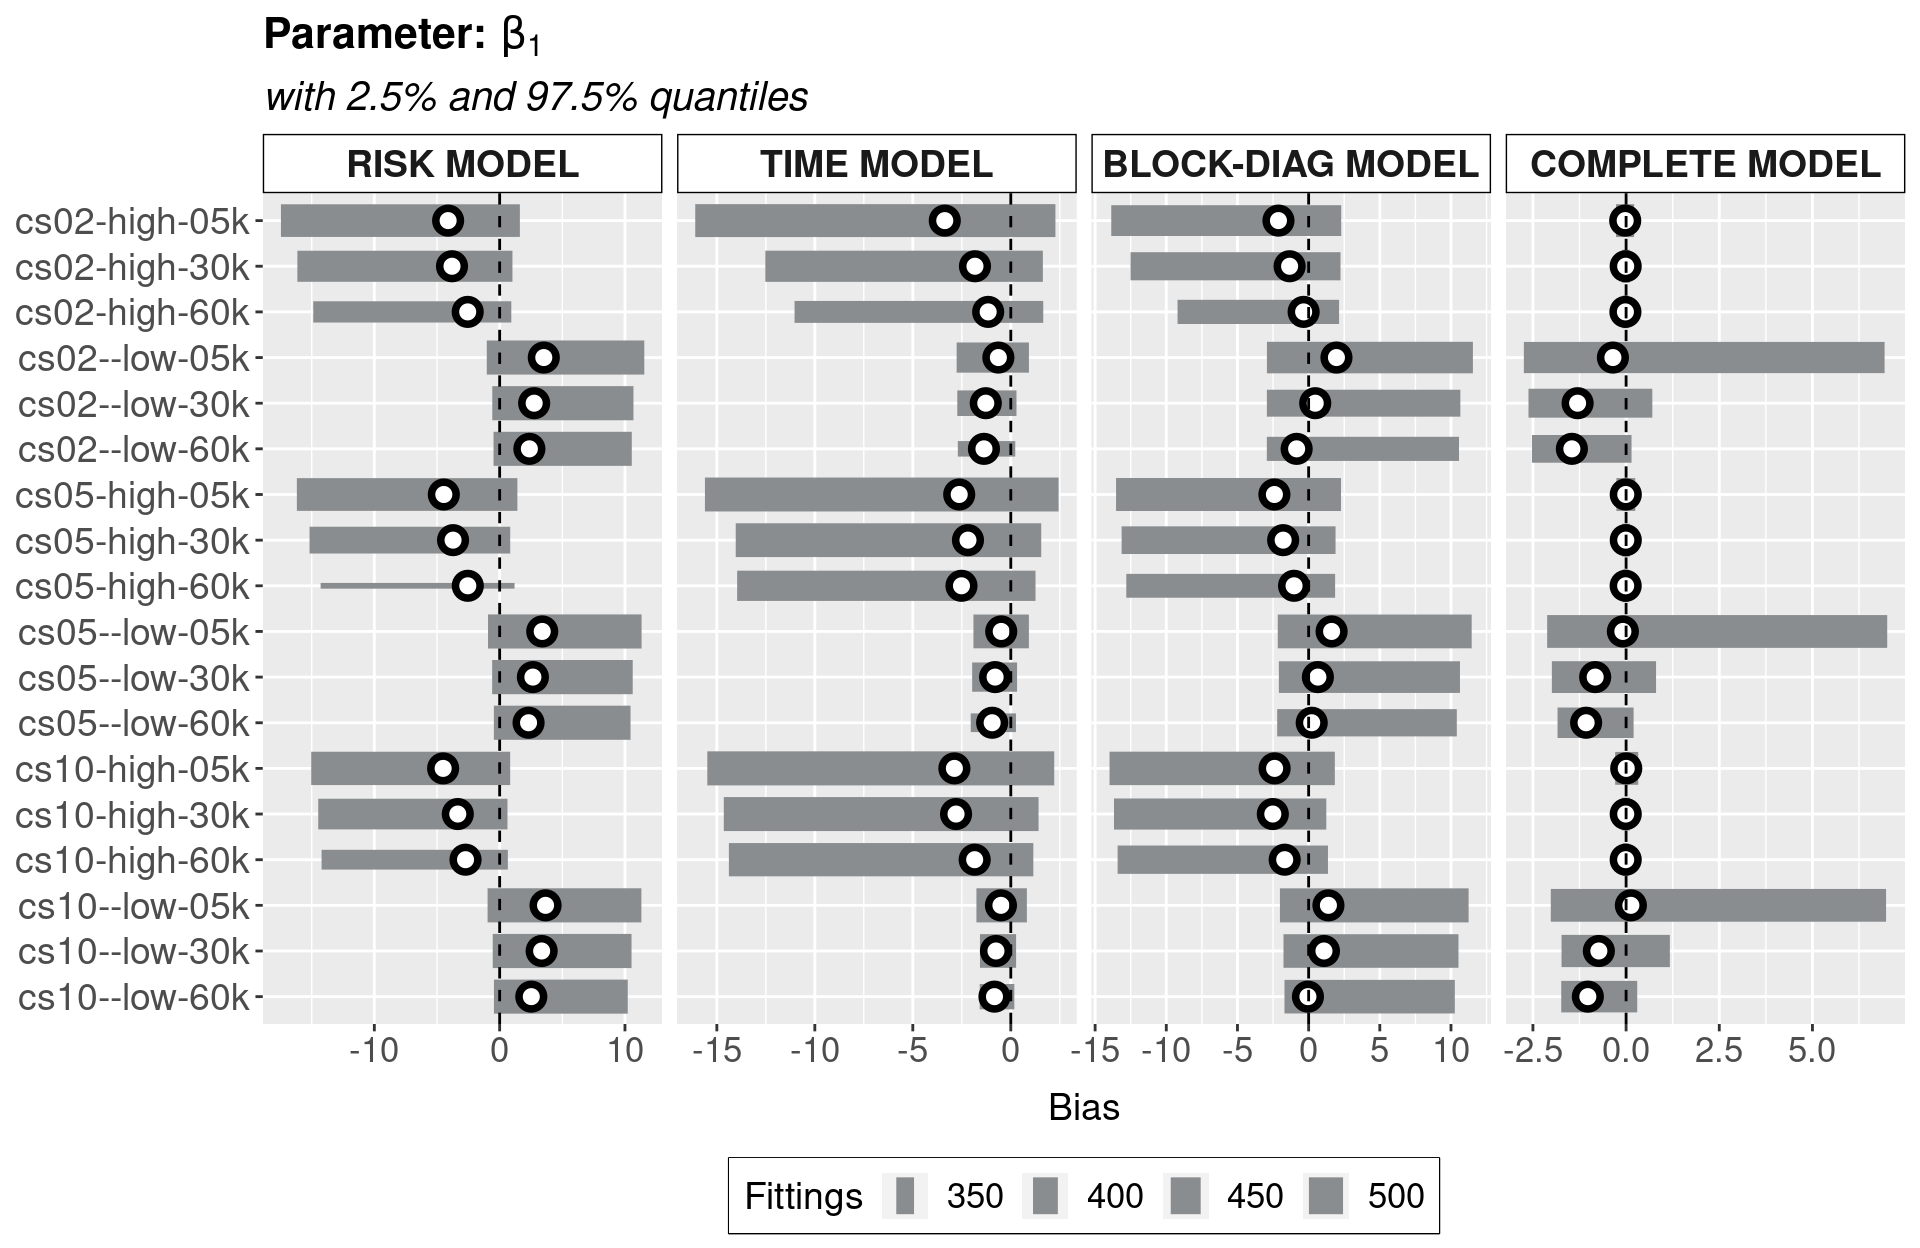
\includegraphics[width=\textwidth]{bias2plot-1.png}\\
 \begin{footnotesize}
  SOURCE: The author (2021).
 \end{footnotesize}
 \label{fig:biasbeta1}
\end{figure}

\begin{figure}[H]
 \setlength{\abovecaptionskip}{.0001pt}
 \caption{PARAMETER \(\beta_{2}\) BIAS WITH 2.5\% AND 97.5\% QUANTILES}
 \vspace{0.2cm}\centering
 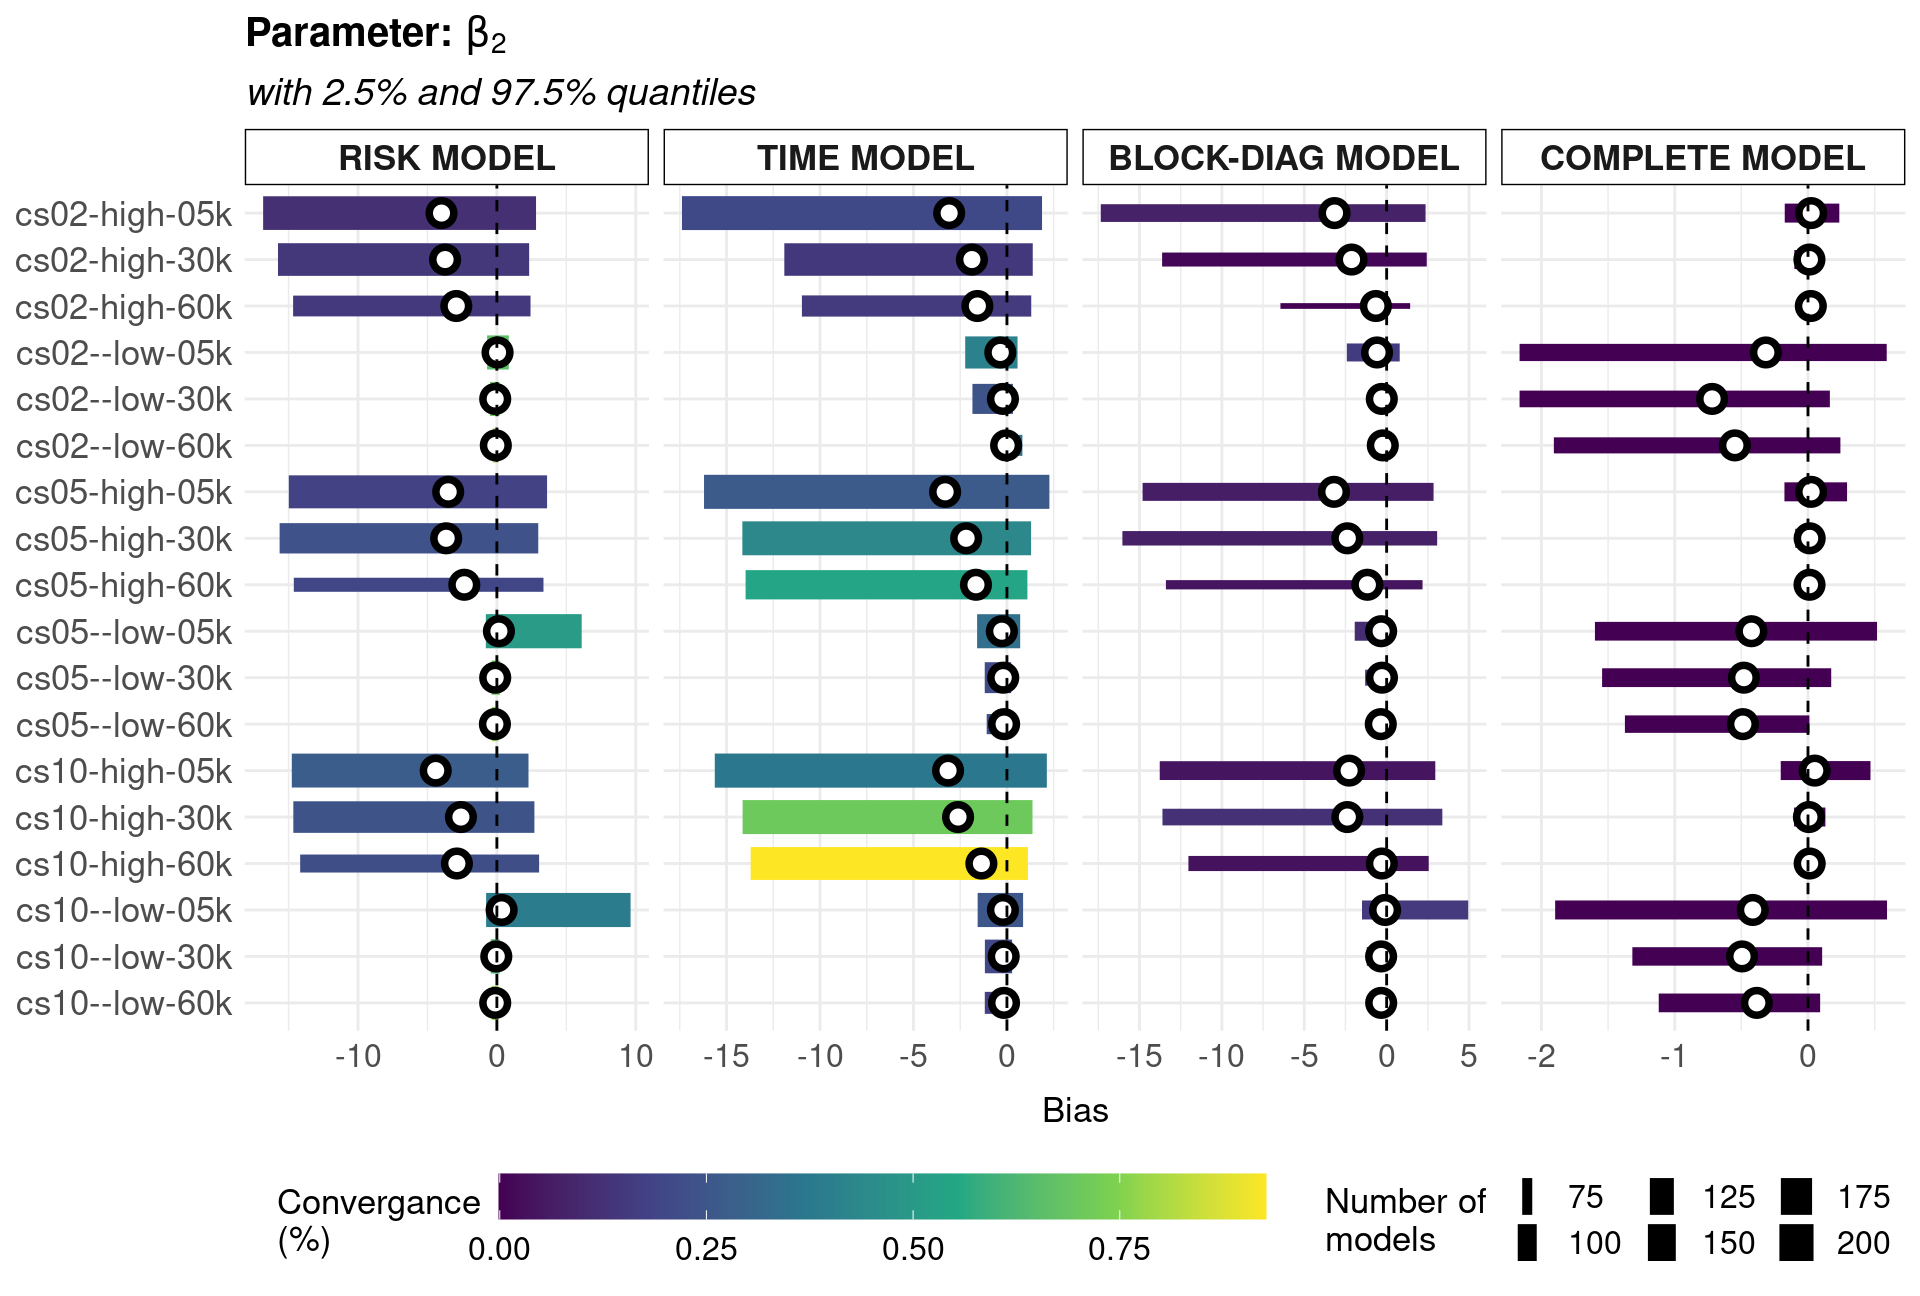
\includegraphics[width=\textwidth]{bias2plot-2.png}\\
 \begin{footnotesize}
  SOURCE: The author (2021).
 \end{footnotesize}
 \label{fig:biasbeta2}
\end{figure}

\begin{figure}[H]
 \setlength{\abovecaptionskip}{.0001pt}
 \caption{PARAMETER \(\gamma_{1}\) BIAS WITH 2.5\% AND 97.5\% QUANTILES}
 \vspace{0.2cm}\centering
 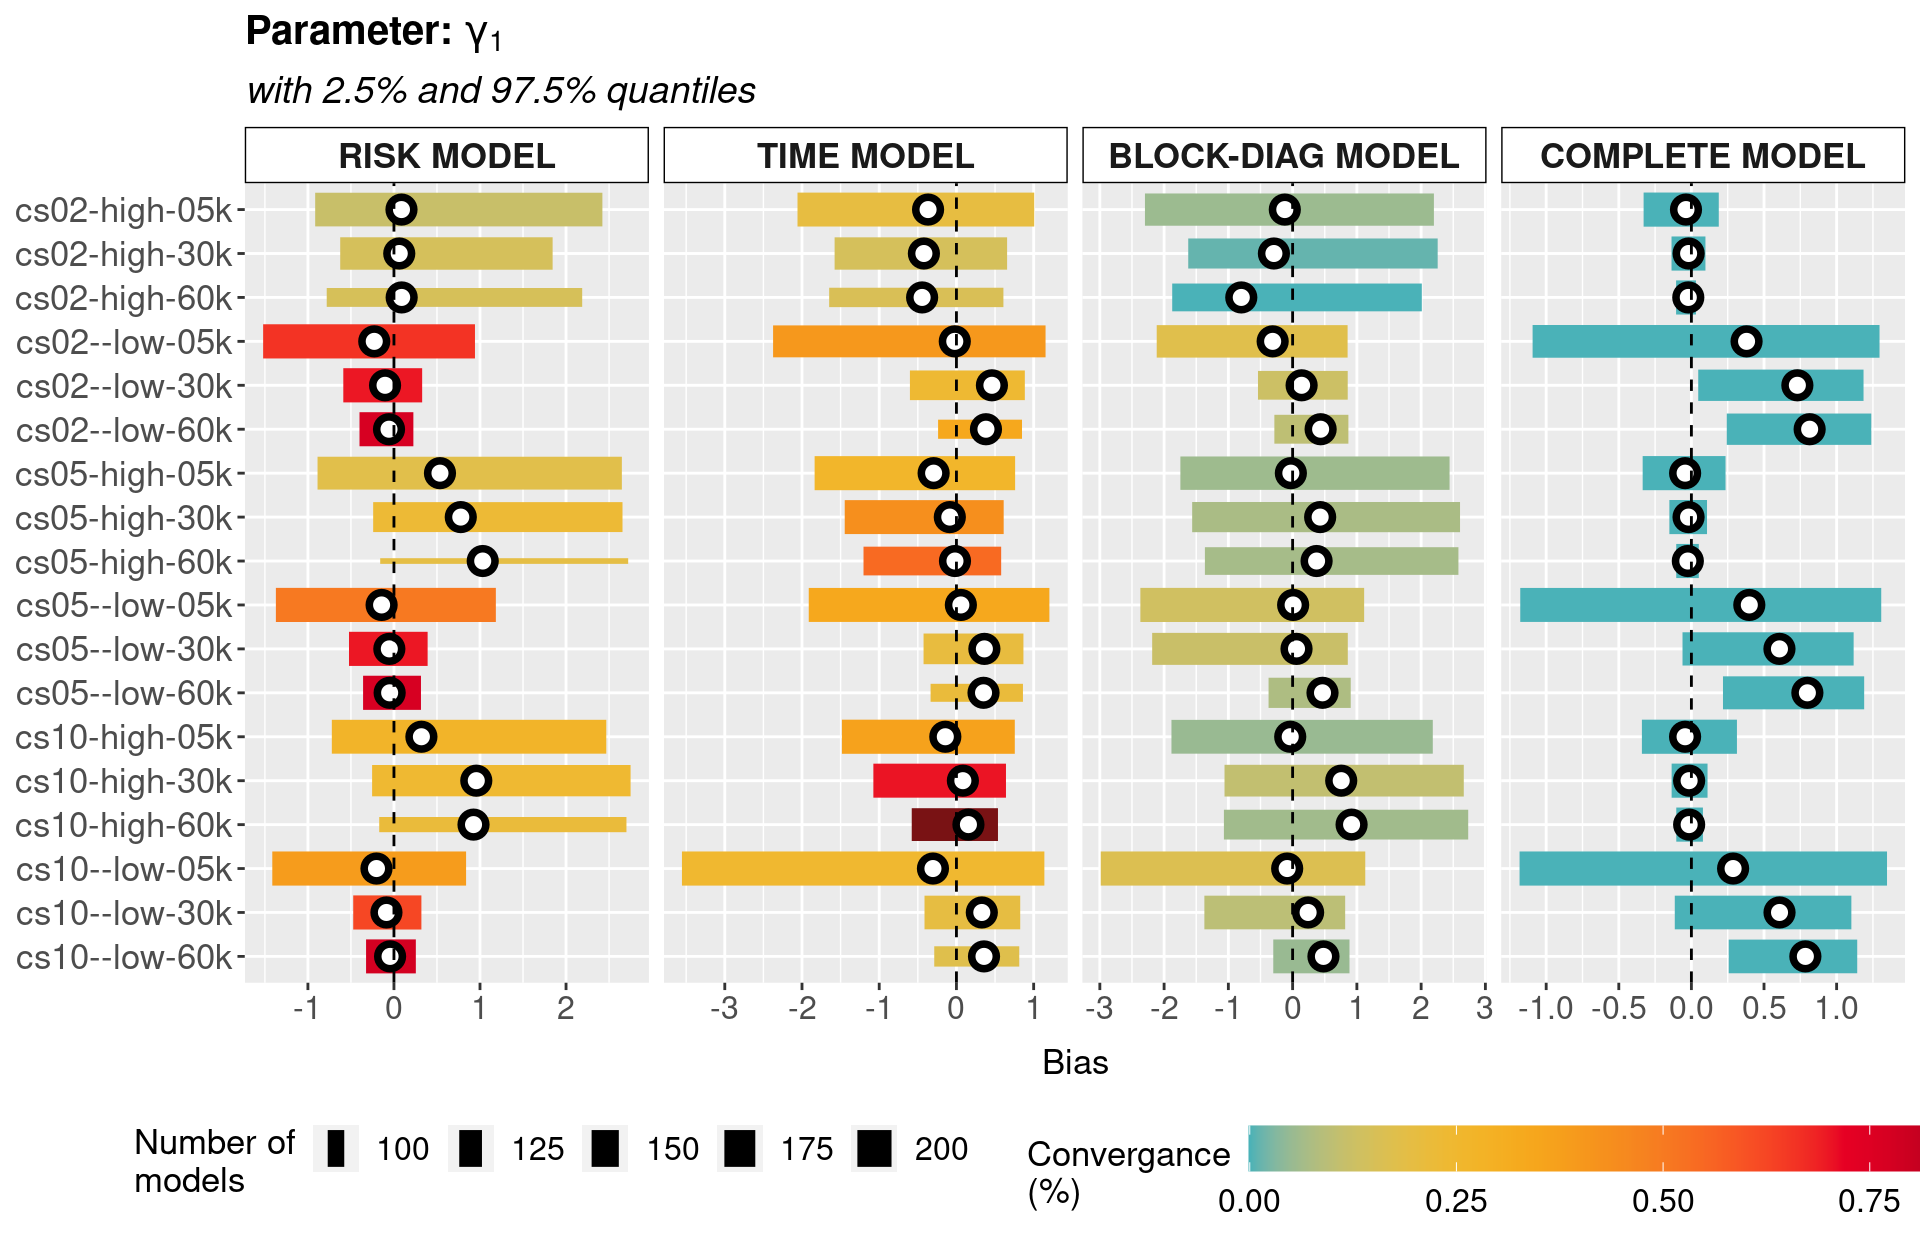
\includegraphics[width=\textwidth]{bias2plot-3.png}\\
 \begin{footnotesize}
  SOURCE: The author (2021).
 \end{footnotesize}
 \label{fig:biasgama1}
\end{figure}

\begin{figure}[H]
 \setlength{\abovecaptionskip}{.0001pt}
 \caption{PARAMETER \(\gamma_{2}\) BIAS WITH 2.5\% AND 97.5\% QUANTILES}
 \vspace{0.2cm}\centering
 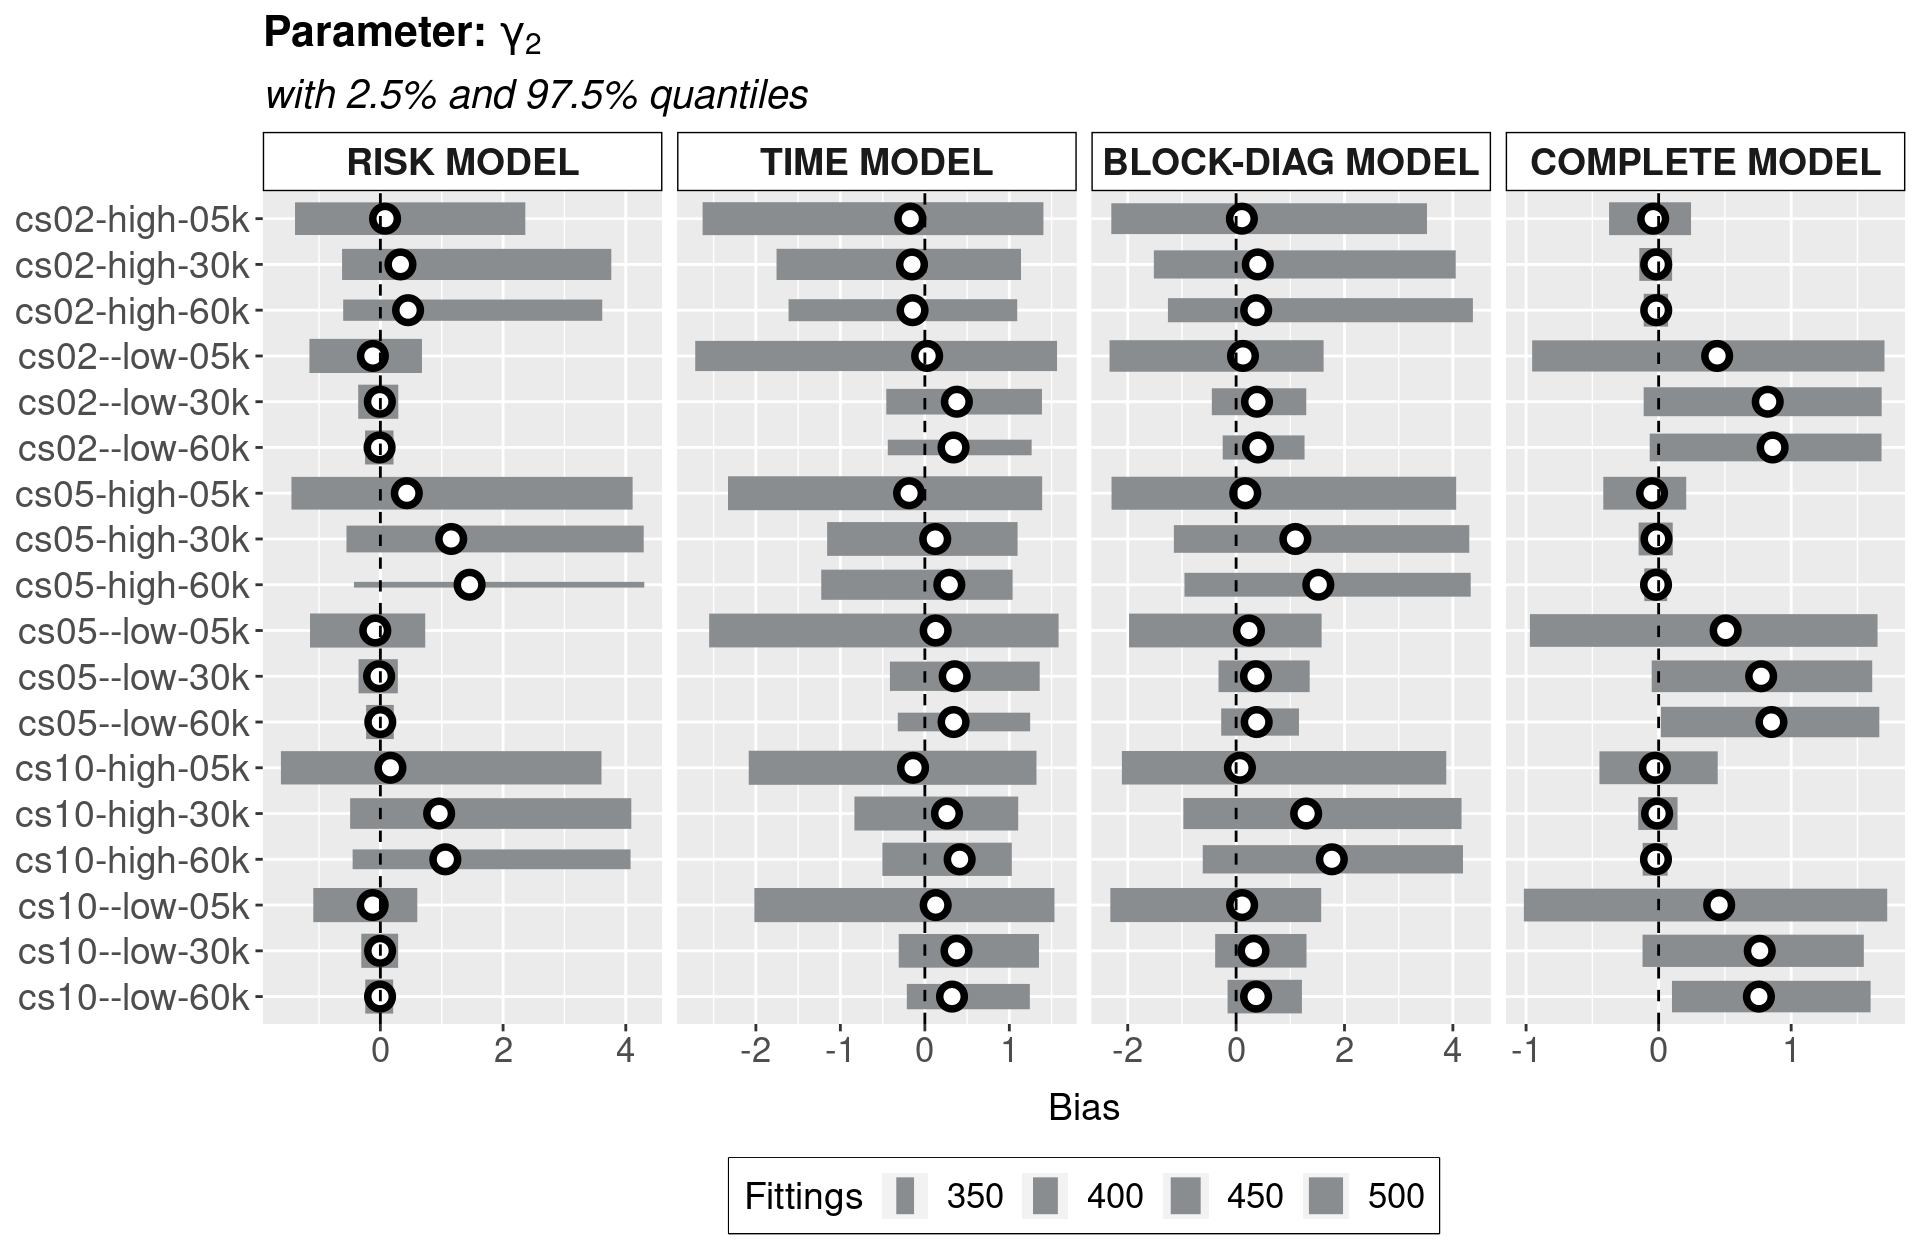
\includegraphics[width=\textwidth]{bias2plot-4.png}\\
 \begin{footnotesize}
  SOURCE: The author (2021).
 \end{footnotesize}
 \label{fig:biasgama2}
\end{figure}

\begin{figure}[H]
 \setlength{\abovecaptionskip}{.0001pt}
 \caption{PARAMETER \(w_{1}\) BIAS WITH 2.5\% AND 97.5\% QUANTILES}
 \vspace{0.2cm}\centering
 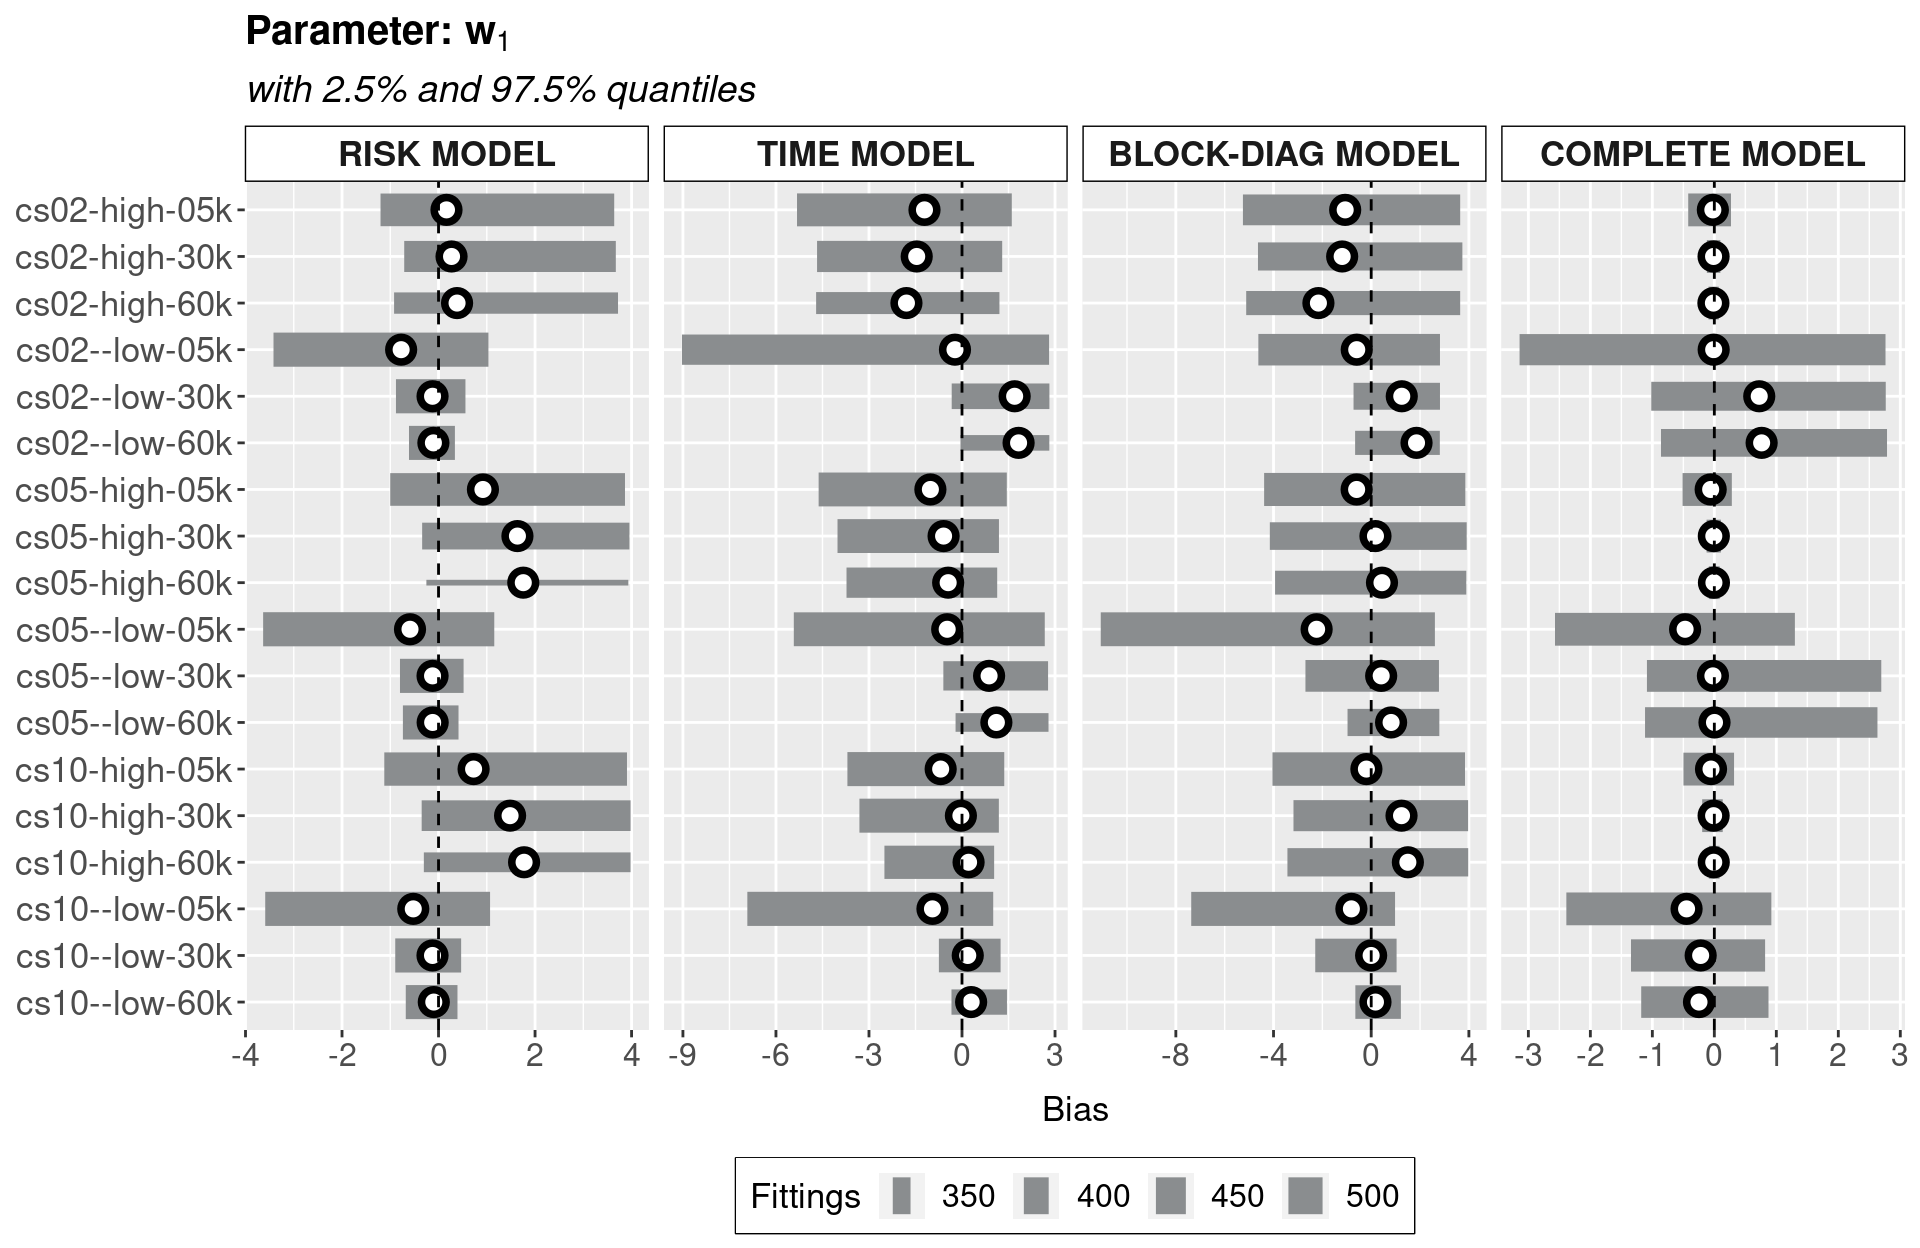
\includegraphics[width=\textwidth]{bias2plot-5.png}\\
 \begin{footnotesize}
  SOURCE: The author (2021).
 \end{footnotesize}
 \label{fig:biasw1}
\end{figure}

\begin{figure}[H]
 \setlength{\abovecaptionskip}{.0001pt}
 \caption{PARAMETER \(w_{2}\) BIAS WITH 2.5\% AND 97.5\% QUANTILES}
 \vspace{0.2cm}\centering
 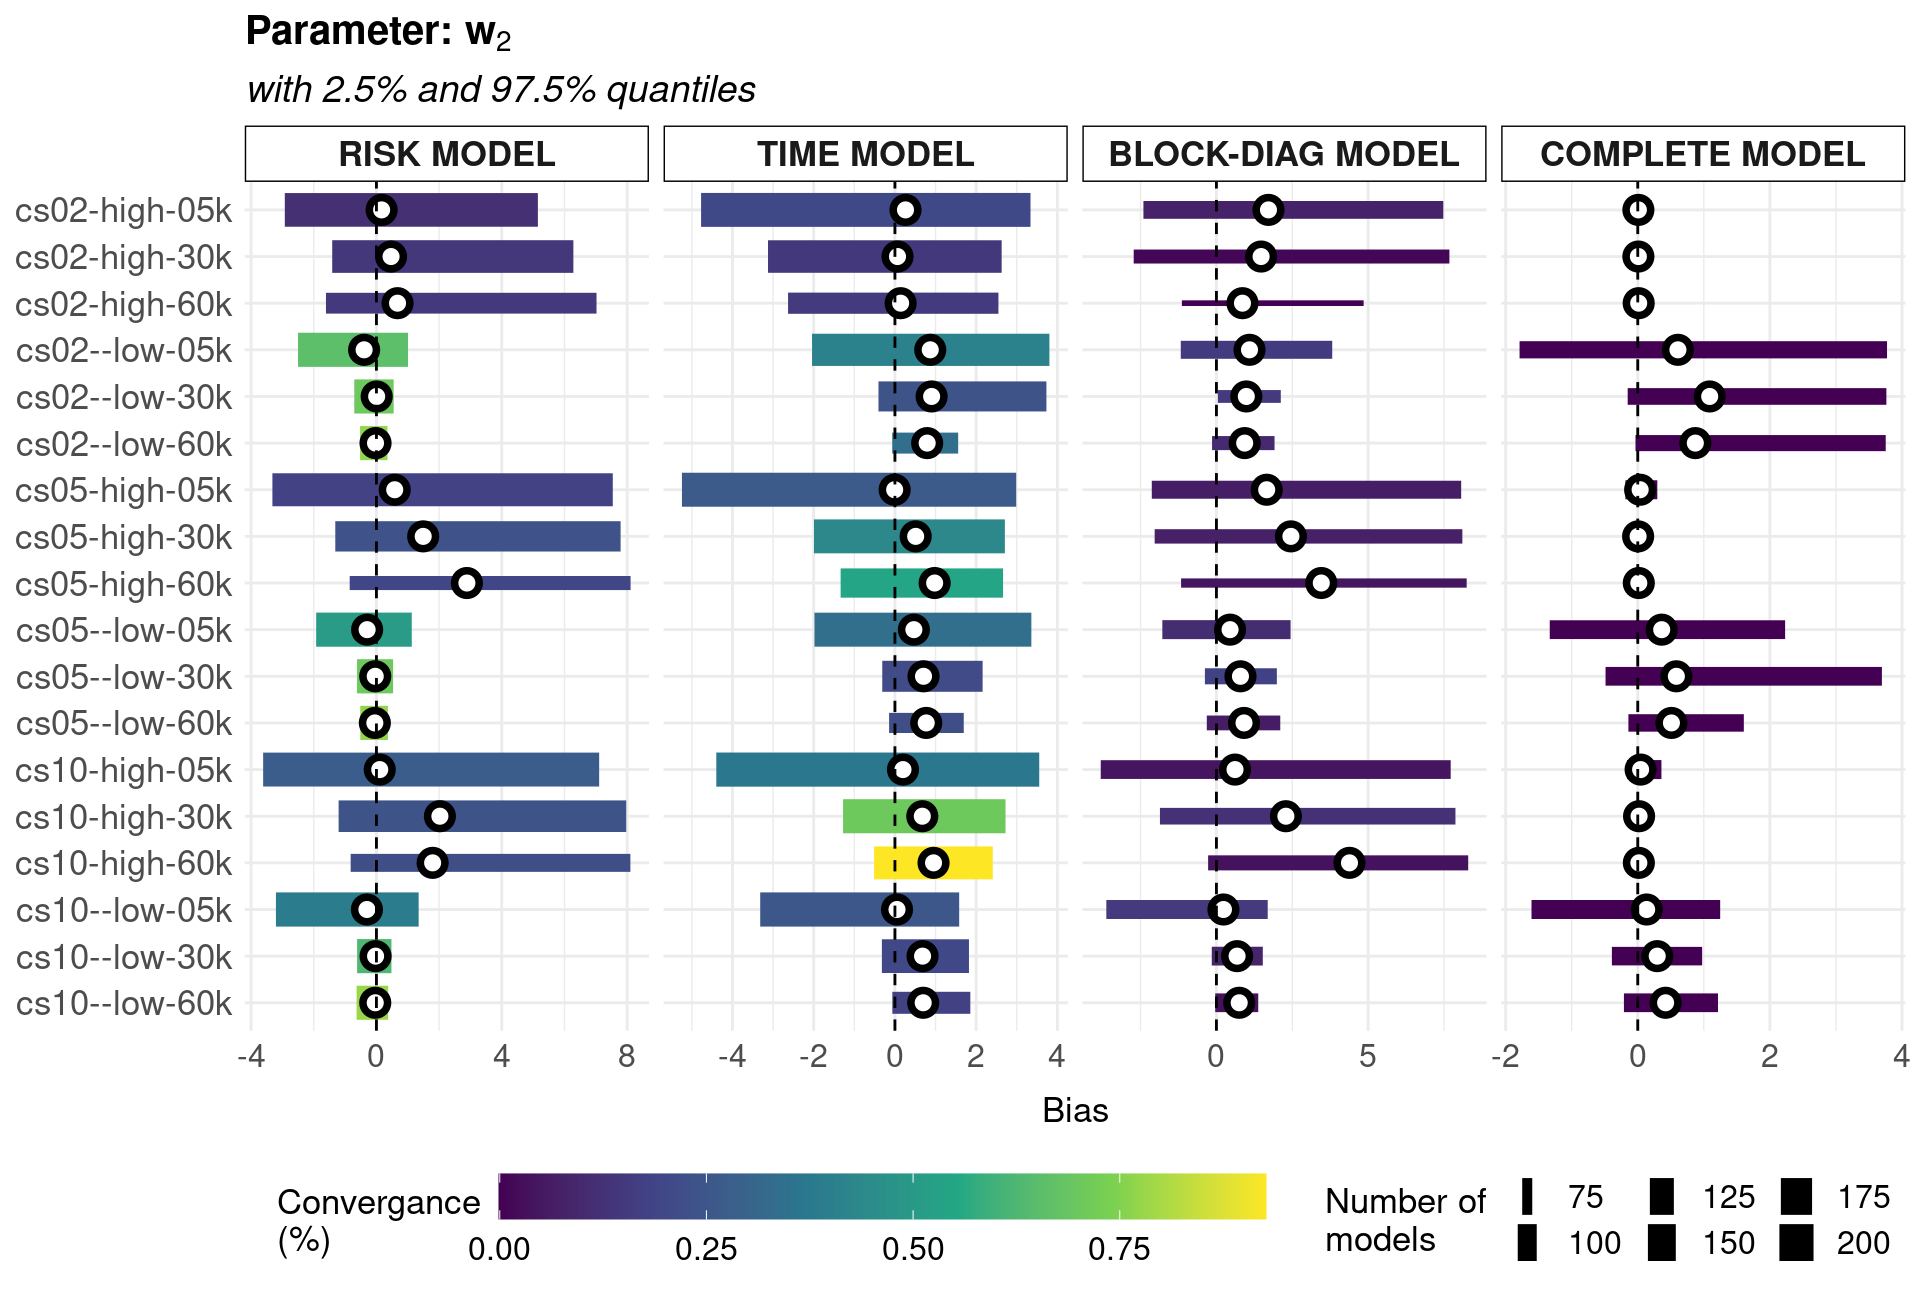
\includegraphics[width=\textwidth]{bias2plot-6.png}\\
 \begin{footnotesize}
  SOURCE: The author (2021).
 \end{footnotesize}
 \label{fig:biasw2}
\end{figure}

\begin{figure}[H]
 \setlength{\abovecaptionskip}{.0001pt}
 \caption{PARAMETER \(\log(\sigma_{1}^{2})\) BIAS WITH 2.5\% AND 97.5\%
          QUANTILES}
 \vspace{0.2cm}\centering
 \includegraphics[width=\textwidth]{bias2plot-7.png}\\
 \begin{footnotesize}
  SOURCE: The author (2021).
 \end{footnotesize}
 \label{fig:biaslogs2_1}
\end{figure}

\begin{figure}[H]
 \setlength{\abovecaptionskip}{.0001pt}
 \caption{PARAMETER \(\log(\sigma_{2}^{2})\) BIAS WITH 2.5\% AND 97.5\%
          QUANTILES}
 \vspace{0.2cm}\centering
 \includegraphics[width=\textwidth]{bias2plot-8.png}\\
 \begin{footnotesize}
  SOURCE: The author (2021).
 \end{footnotesize}
 \label{fig:biaslogs2_2}
\end{figure}

\begin{figure}[H]
 \setlength{\abovecaptionskip}{.0001pt}
 \caption{PARAMETER \(\log(\sigma_{3}^{2})\) BIAS WITH 2.5\% AND 97.5\%
          QUANTILES}
 \vspace{0.2cm}\centering
 \includegraphics[width=\textwidth]{bias2plot-9.png}\\
 \begin{footnotesize}
  SOURCE: The author (2021).
 \end{footnotesize}
 \label{fig:biaslogs2_3}
\end{figure}

\begin{figure}[H]
 \setlength{\abovecaptionskip}{.0001pt}
 \caption{PARAMETER \(\log(\sigma_{4}^{2})\) BIAS WITH 2.5\% AND 97.5\%
          QUANTILES}
 \vspace{0.2cm}\centering
 \includegraphics[width=\textwidth]{bias2plot-10.png}\\
 \begin{footnotesize}
  SOURCE: The author (2021).
 \end{footnotesize}
 \label{fig:biaslogs2_4}
\end{figure}

\begin{figure}[H]
 \setlength{\abovecaptionskip}{.0001pt}
 \caption{PARAMETER \(z(\rho_{12})\) BIAS WITH 2.5\% AND 97.5\%
          QUANTILES}
 \vspace{0.2cm}\centering
 \includegraphics[width=\textwidth]{bias2plot-11.png}\\
 \begin{footnotesize}
  SOURCE: The author (2021).
 \end{footnotesize}
 \label{fig:biasrhoz12}
\end{figure}

\begin{figure}[H]
 \setlength{\abovecaptionskip}{.0001pt}
 \caption{PARAMETER \(z(\rho_{34})\) BIAS WITH 2.5\% AND 97.5\%
          QUANTILES}
 \vspace{0.2cm}\centering
 \includegraphics[width=\textwidth]{bias2plot-12.png}\\
 \begin{footnotesize}
  SOURCE: The author (2021).
 \end{footnotesize}
 \label{fig:biasrhoz34}
\end{figure}

\begin{figure}[H]
 \setlength{\abovecaptionskip}{.0001pt}
 \caption{PARAMETERS
          \(\{z(\rho_{13}),~z(\rho_{24}),~z(\rho_{14}),~z(\rho_{23})\}\)
          BIAS WITH 2.5\% AND 97.5\% QUANTILES}
 \vspace{0.2cm}\centering
 \includegraphics[width=\textwidth]{bias2plot-13.png}\\
 \begin{footnotesize}
  SOURCE: The author (2021).
 \end{footnotesize}
 \label{fig:biasrhoz4}
\end{figure}

\end{apendicesenv}
% ----------------------------------------------------------------------
% \begin{anexosenv}
% \partanexos
% \addcontentsline{toc}{chapter}{\hspace{2.105cm}ANNEX}
% \renewcommand{\ABNTEXchapterfontsize}{\ABNTEXsectionfont}
% \end{anexosenv}
%-----------------------------------------------------------------------
\phantompart
\printindex
%-----------------------------------------------------------------------
\end{document}
% END ==================================================================

% ----------------------------------------------------------------------
% pacote para fazer o checkmark
\usepackage{pifont} % http://ctan.org/pkg/pifont
\newcommand{\cmark}{\ding{51}}%
\newcommand{\xmark}{\ding{55}}%
% ----------------------------------------------------------------------
\usepackage{amsmath}
\usepackage{blkarray}
\usepackage{amsfonts}
\usepackage{amssymb}
\usepackage{pdfpages}
% \usepackage{times}
% \usepackage{helvet}
% \renewcommand{\familydefault}{\sfdefault}
% ----------------------------------------------------------------------
\NewDocumentCommand\cc{+u{\cc}}{\ignorespaces}
% ----------------------------------------------------------------------
% controle do espaçamento entre um parágrafo e outro:
\setlength{\parskip}{0.2cm} % tente também \onelineskip
% ----------------------------------------------------------------------
\titulo{MODELING THE CUMULATIVE INCIDENCE FUNCTION OF CLUSTERED
  COMPETING RISKS DATA: A MULTINOMIAL GLMM APPROACH}
\autor{HENRIQUE APARECIDO LAUREANO}
\data{2021}
\instituicao{FEDERAL UNIVERSITY OF PARANÁ}
\orientador{Prof. PhD Wagner Hugo Bonat}
\coorientador{Prof. PhD Paulo Justiniano Ribeiro Jr}
\tipotrabalho{Dissertação (mestrado)}
\preambulo{\small{Thesis presented to the Graduate Program of Numerical
    Methods in Engineering, Concentration Area in Mathematical
    Programming: Statistical Methods Applied in Engineering, Federal
    University of Paran\'{a}, as part of the requirements to the
    obtention of the Master's Degree in Sciences.}}
% ----------------------------------------------------------------------
% informações do PDF
\makeatletter
\hypersetup{
  % pagebackref=true,
  pdftitle={\@title},
  pdfauthor={\@author},
  pdfsubject={\imprimirpreambulo},
  % pdfkeywords = {}{}{}{},
  colorlinks=true, % false: boxed links; true: colored links
  linkcolor=blue, % color of internal links
  citecolor=blue, % color of links to bibliography
  filecolor=magenta, % color of file links
  urlcolor=blue,
  bookmarksdepth=4
}
\addto\captionsenglish{
  % adjusts names from abnTeX2
  \renewcommand{\folhaderostoname}{Title page}
  \renewcommand{\epigraphname}{Epigraph}
  \renewcommand{\dedicatorianame}{Dedication}
  \renewcommand{\errataname}{Errata sheet}
  \renewcommand{\agradecimentosname}{Acknowledgements}
  \renewcommand{\anexoname}{ANNEX}
  \renewcommand{\anexosname}{Annex}
  \renewcommand{\apendicename}{APPENDIX}
  \renewcommand{\apendicesname}{Appendix}
  \renewcommand{\orientadorname}{Supervisor:}
  \renewcommand{\coorientadorname}{Co-supervisor:}
  \renewcommand{\folhadeaprovacaoname}{Approval}
  \renewcommand{\resumoname}{Abstract}
  \renewcommand{\listadesiglasname}{List of abbreviations and acronyms}
  \renewcommand{\listadesimbolosname}{List of symbols}
  \renewcommand{\fontename}{Source}
  \renewcommand{\notaname}{Note}
  % adjusts names used by \autoref
  \renewcommand{\pageautorefname}{page}
  \renewcommand{\chapterautorefname}{Chapter}
  \renewcommand{\sectionautorefname}{Section}
  \renewcommand{\subsectionautorefname}{subsection}
  \renewcommand{\subsubsectionautorefname}{subsubsection}
  \renewcommand{\paragraphautorefname}{subsubsubsection}
}
\makeatother
% ----------------------------------------------------------------------
\graphicspath{{figures/}}
% ----------------------------------------------------------------------
\begin{document}
\selectlanguage{english}
% adequando o uppercase titulo dos elementos nas suas respectivas
% legendas
\renewcommand{\tablename}{TABLE }
\renewcommand{\figurename}{FIGURE }
% ----------------------------------------------------------------------
\frenchspacing % retira espaço extra obsoleto entre as frases
% ----------------------------------------------------------------------
% capa
\tikz[remember picture,overlay] \node[opacity=1,inner sep=0pt] at
(current page.center){
  \includegraphics[width=\paperwidth,
  height=\paperheight]{Figuras/ufpr_bg}};
% ----------------------------------------------------------------------
\imprimircapa
% ----------------------------------------------------------------------
% folha de rosto
\imprimirfolhaderosto
% ----------------------------------------------------------------------
% \begin{dedicatoria}
%   \vspace*{\fill}
%   ...
%   \vspace*{\fill}
% \end{dedicatoria}
% ----------------------------------------------------------------------
% ficha catalográfica

% \begin{fichacatalografica}
%   \includepdf{ficha.pdf}
% \end{fichacatalografica}
% ----------------------------------------------------------------------
% inserir folha de aprovação
% \begin{folhadeaprovacao}
%   \includepdf{termo.pdf}
% \end{folhadeaprovacao}
\begin{folhadeaprovacao}
 \begin{center}
   {\ABNTEXchapterfont\large\imprimirautor}

   \vspace*{\fill}\vspace*{\fill}
   \begin{center}
     \ABNTEXchapterfont\bfseries\large\imprimirtitulo
   \end{center}
   \vspace*{\fill}

    \hspace{.45\textwidth}
    \begin{minipage}{.5\textwidth}
       \imprimirpreambulo
    \end{minipage}
   \vspace*{\fill}
 \end{center}

 Master thesis approved. XXX XX, 2021.

  \assinatura{\textbf{\imprimirorientador}\\ Supervisor}
  \assinatura{\textbf{Prof. PhD Paulo Justiniano Ribeiro Jr}\\
    Co-supervisor}
  \assinatura{\textbf{Prof. PhD \(\dots\)}\\
    Internal Examinator - PPGMNE}
  \assinatura{\textbf{Prof. PhD \(\dots\)}\\
    Internal Examinator - PPGMNE}
  \assinatura{\textbf{Prof. PhD \(\dots\)}\\External Examiner - }

  \begin{center}
   \vspace*{0.5cm}
   {\large CURITIBA}
   \par
   {\large\imprimirdata}
   \vspace*{1cm}
 \end{center}

\end{folhadeaprovacao}
% ----------------------------------------------------------------------
\begin{dedicatoria}
  \vspace*{22.7cm}
  \begin{flushright}
    \begin{minipage}[H]{4.5cm}
      {To Celita and Olivio}
    \end{minipage}
  \end{flushright}
\end{dedicatoria}
% ----------------------------------------------------------------------
\begin{agradecimentos}
 As Moro once said, I am thankful for everything and everyone.

 Today is the shadow of tomorrow. Today is the present future of
 yesterday. Yesterday is the shadow of today. The wisdom of the past is
 the light of the past. The light of the future casts the shadows of
 tomorrow.
\end{agradecimentos}

\begin{epigrafe}
  \vspace*{\fill}
  \begin{flushright}
    \textit{"It's not supposed to be easy."\\
             (Gregg Popovich)}
              % on Sao Antonio Spurs \(\times\) Oklahoma City Thunder,
              % first game of the 2012 Western Conference Finais
  \end{flushright}
\end{epigrafe}
% ----------------------------------------------------------------------
\newpage
\setlength{\absparsep}{18pt} % ajusta o espaçamento dos parágrafos do
                             % resumo
\setlength{\abstitleskip}{1cm} % adiciona mais um cm após o 'titulo' do
                               % resumo para ficar com 2cm
\begin{resumo}[]
  \vspace{-2cm}
  \begin{center}
    \bfseries{\large{\textsf{ABSTRACT}}}
  \end{center}
  \vspace{0.3cm}

  Clustered competing risks data is a special case of failure time
  data. Besides the cluster structure which implies a within-cluster
  dependence between its elements, this kind of data is characterized by
  1) multiple causes/variables competing to be the one responsible for
  the occurrence of an event, a failure; and 2) censorship, when the
  event of interest happens for none of the competing causes, in the
  study period.

  To handle this type of data, we propose a latent-effects framework, a
  generalized linear mixed model (GLMM), instead of a usual survival
  model. In survival analysis, the modeling is done by means of the
  hazard rate, and the within-cluster dependence accommodation generates
  a complicated likelihood function sometimes intractable. What we do
  here is to model the clustered competing causes in the probability
  scale, in terms of the cumulative incidence function (CIF) of each
  competing cause. In our framework, we suppose a multinomial
  probability distribution for the competing causes and censorship,
  conditioned on the latent effects (within-cluster dependence). The
  latent effects are accommodated by a multivariate Gaussian
  distribution and are modeled by the parameters of its covariance
  matrix. These probability distributions are connected by the CIF,
  modeled here following the specification in \citeonline{SCHEIKE},
  based on the CIF decomposition as the product of an instantaneous risk
  level function with a trajectory time level function. The latent
  effects are inserted in those level functions.  To make the estimation
  of the parameters of this model the most efficient as possible, we use
  the template model builder (TMB) \cite{TMB}. With this R \cite{R21}
  package, we have our log-likelihood function written in C++, we have
  access to state-of-the-art computational libraries, an efficient
  Laplace approximation implementation for the latent-effects, and an
  automatic differentiation (AD) routine, the state-of-the-art in
  derivatives computation. To check the estimability of our model a
  large simulation study is performed, based on different latent
  structure formulations, with the aim to verify which one is most
  adequate. The model presents to be of difficult estimation, with our
  results converging to a latent restructure where the risk and
  trajectory time levels are correlated. In scenarios with high CIF the
  model exhibits good results, but with an excessive variance, showing
  that improvements are necessary.
  
  In scenarios with high CIF the model exhibits good results, but with
  an excessive variance, showing that improvements are necessary.
  
  \textbf{Keywords}: Clustered competing risks.
                     Within-cluster dependence.
                     Multinomial generalized linear mixed model (GLMM).
                     TMB: Template Model Builder.
                     Laplace approximation.
                     Automatic differentiation (AD).
\end{resumo}
% ----------------------------------------------------------------------
\newpage
\setlength{\absparsep}{18pt} % ajusta o espaçamento dos parágrafos do
                             % resumo
\setlength{\abstitleskip}{1cm} % adiciona mais um cm após o 'titulo' do
                               % resumo para ficar com 2cm
\begin{resumo}[]
  \begin{otherlanguage*}{brazil}
    \vspace{-2cm}
    \begin{center}
      \bfseries{\large{\textsf{RESUMO}}}
    \end{center}
    \vspace{0.3cm}

    \textbf{Palavras-chave}: Riscos competitivos agrupados.
                             Depend\^{e}ncia intra-cluster.
                             Modelo linear generalizado misto
                             multinomial (MLGM).
                             TMB: Template Model Builder.
                             Aproxima\c{c}\~{a}o de Laplace.
                             Diferencia\c{c}\~{a}o autom\'{a}tica.
  \end{otherlanguage*}
\end{resumo}
% ----------------------------------------------------------------------
\pdfbookmark[0]{\listfigurename}{lof}
\listoffigures*
\cleardoublepage
% ----------------------------------------------------------------------
%% \pdfbookmark[0]{\listtablename}{lot}
%% \listoftables*
%% \cleardoublepage
% ----------------------------------------------------------------------
\makeatletter
\renewcommand\numberline[1]{
	\leftskip -0.7em
	\rightskip 1.6em
	\parfillskip -\rightskip
	\parindent 0em
	\@tempdima 2.0em
	\vspace{0em}
  \advance\leftskip \@tempdima \null\nobreak\hskip -\leftskip
	ALGORITHM \normalfont #1 ~~ }
\makeatother
% ----------------------------------------------------------------------
\pdfbookmark[0]{\listalgorithmname}{loa}
\listofalgorithms
\cleardoublepage
% ----------------------------------------------------------------------
\makeatletter
\def\numberline#1{\hb@xt@\@tempdima{#1\hfil}}
\makeatother
% ----------------------------------------------------------------------
% \begin{siglas}
% \item[Fig.] Area of the $i^{th}$ component
% \item[456] Isto é um número
% \item[123] Isto é outro número
% \item[lauro cesar] este é o meu nome
% \end{siglas}
% ----------------------------------------------------------------------
% \begin{simbolos}
% \item[\(\mathbb{E}(\cdot)\)] The mathematical expectation of a random
%   variable \(\cdot\)
% \end{simbolos}
% ----------------------------------------------------------------------
\pdfbookmark[0]{\contentsname}{toc}
\tableofcontents*
\cleardoublepage
% ----------------------------------------------------------------------
\makepagestyle{abntheadings}
\makeevenhead{abntheadings}{\ABNTEXfontereduzida\thepage}{}{}
\makeoddhead{abntheadings}{}{}{\ABNTEXfontereduzida\thepage}
\makeheadrule{abntheadings}{\textwidth}{0in}
% ----------------------------------------------------------------------
\textual
% ----------------------------------------------------------------------
\chapter{Introduction}
\label{cap:intro}
Consider a cluster of random variables representing the time until the
occurrence of some event. These random variables are assumed to be
correlated, i.e. for some biological or environmental reason it is not
adequate to assume independence between them. Also, we may be interested
in the occurrence of not only one specific event, having in practice a
competition of events to see which one happens first, if it
happens. Such events may also be of low probability albeit severe
consequences, this is the moment when the cluster correlation makes its
difference: the occurrence of an event in a cluster member should affect
the probability of the same happening in the others.

A realistic context that fits perfectly with the framework described
above is the study of disease incidence in family members, where each
member is indexed by a random variable and each cluster consists of a
familiar structure. More specifically, we are interested in what is
called \textit{family studies}. Besides the dependence between family
members, this kind of data is characterized by being consisted of big
samples, or even a population, and having a lot of clusters/families of
small size. The inspiration to these kinds of problems came from the
work developed in \citeonline{SCHEIKE}, where they studied breast cancer
incidence in mothers and daughters but using a nontrivial estimation
framework. Based on that, the aim of this thesis is to propose a simpler
estimation framework taking advantage of several \textit{state-of-art}
computational libraries and see how far we can go in several
scenarios. Until now we have just contextualized, we still need to
introduce the methodology. To do this, some definitions and theoretical
contexts are welcome.

When the object under study is a random variable representing the time
until some event occurs, we are in the field of \textit{failure time
data} \cite{kalb&prentice}. The occurrence of an event is generally
denoted \textit{failure}, and major areas of application are biomedical
studies and industrial life testing. In this thesis, we maintain our
focus on the former. As common in science, same methodologies can
receive different names depending on the area. In industrial life
testing is performed what is called a \textit{reliability analysis}; in
biomedical studies is performed what is called
\textit{survival analysis}. Generally, the term \textit{survival} is
applied when we are interested in the occurrence of only one event, a
\textit{failure time process}. When we are interested in the occurrence
of more than one event we enter in the yard of \textit{competing risks}
and \textit{multistate} models. A visual aid is presented on
\autoref{fig:intro1} and a comprehensive reference is
\citeonline{kalb&prentice}.

Failure time and competing risks processes may be seen as particular
cases of a multistate model. Besides the number of events (states) of
interest, the main difference between a multistate model and its
particular cases is that only in the multistate scenario we may have
transient states, using a \textit{stochastic process} language. In the
particular cases, all states besides the initial state 0, are absorbents
- once you reached it you do not leave. The simplest multistate model
that exemplify this behavior is the illness-death model,
\autoref{fig:intro1}~C), where a patient (initially in state 0) can get
sick (state 1) or die (state 2); if sick it can recover (returns to
state 0) or die. We work in this thesis only with competing risks
processes, and for each patient we need the time (age) until the
occurrence, or not, of the event.

\begin{figure}[H]
 \setlength{\abovecaptionskip}{.0001pt}
 \caption{ILLUSTRATION OF MULTISTATE MODELS FOR A A) FAILURE TIME
          PROCESS; B) COMPETING RISKS PROCESS; AND C) ILNESS-DEATH
          MODEL, THE SIMPLEST MULTISTATE MODEL}
 \vspace{0.5cm}\centering
 \tikzfig{fig1}\\
 \vspace{0.5cm}
 \begin{footnotesize}
  SOURCE: The author~(2021).
 \end{footnotesize}
 \label{fig:intro1}
\end{figure}

When for some known or unknown reason we are not able to see the
occurrence of an event, we have what is denoted \textit{censorship}.
Still in the illness-death model, during the period of follow up the
patient may not get sick or die, staying at state 0. This is denoted
\textit{right-censorship}; if a patient is in state 1 at the end of the
study, we are \textit{censored} to see him reaching the state 2 or
returning to state 0. This is the inherent idea to censorship and must
be present in the modeling framework, thus arriving in the so-called
\textit{survival models} \cite{kalb&prentice}.

A survival model deals with the survival experience. Usually, the
survival experience is modeled in the \textit{hazard} (failure rate)
scale and it can be expressed for a subject \(i\) as
\begin{equation}
  \lambda(t \mid \bm{x}_{i}) =
  \lambda_{0}(t) \times c(\bm{x}_{i} \bm{\beta})
  \quad \text{at time}~t,
  \label{eq:intro1}
\end{equation}
i.e. as the product of an arbitrary baseline hazard function
\(\lambda_{0}(\cdot)\), with a specific function form \(c(\cdot)\), that
will depend on the probability distribution to be chosen for the failure
time and on predictors/covariates/explanatory/independent variables
\(\bm{x}_{i} = [x_{1}~\dots~x_{p}]\), where \(\bm{\beta}^{\top} =
[\beta_{1}~\dots~\beta_{p}]\) is the parameters vector.

This structure is specified for a failure time process, as in
\autoref{fig:intro1}~A). Nevertheless, the idea is easy to extend. We
basically have the \autoref{eq:intro1}'s model to each cause-specific
(in a competing risks process) or transition (in a multistate process).
For competing risks, the probable most famous approach is the
\citeonline{fine&gray} subdistribution model. A complete and extensive
detailing can be, again, found in \citeonline{kalb&prentice}.

In this work we approach the case of clustered competing risks. Besides
the cause-specific structure, we have to deal with the fact that the
events are happening in related individuals. This configures what is
denoted \textit{family studies}, i.e. we have a cluster/group/family
dependence that needs to be considered, accommodated, and modeled. This,
possible, dependence is something that we do not actually measure but
know (or just suppose) that exists. In the statistical modeling language
this characteristic receives the name of \textit{random} or
\textit{latent effect}.

A survival model with a latent effect, association, or unobserved
heterogeneity, is denoted \textit{frailty model}
\cite{frailty78,frailty79,liang95,petersen98}. In its simplest form, a
frailty is an unobserved random proportionality factor that modifies the
hazard function of an individual, or of related individuals. Frailty
models are extensions of \autoref{eq:intro1}'s model, and its use
implies challengeable likelihood functions (statistical objective
functions) and inference routines done via elaborated and slow
expectation–maximization (EM) algorithms \cite{nielsen92,klein92} or
inefficient Markov chain Monte Carlo (MCMC) schemes \cite{hougaard00}.
With multiple survival experiences, the general idea is the same but
with even more challengeable likelihoods
\cite{prentice78,larson85,kuk92,therneau00}.

In the competing risks setting, the hazard scale (focusing on the
cause-specific hazard) is not the only possible scale to work on. A more
attractive possibility is to work on the probability scale
\cite{andersen12}, focusing on the cause-specific cumulative incidence
function (CIF). Besides the within-family dependence, in family studies
there is often a strong interest in describing age at disease onset,
which is directly described by the cause-specific CIF. The CIF is the
cumulative probability of experiencing a failure by a given competing
cause along the time. Therefore, making the probability scale a more
attractive and logical choice. Since the CIF plays a central role in
this master thesis, it will be formally defined later in a place with
greater emphasis.

Besides the CIF specification itself, the known works with clustered
competing risks data in the probability scale, differ in terms of
likelihood construction and parameters estimation routines. There is a
lack of methodology predominance in the literature, but with its
majority being designed for bivariate CIFs, where increasing the CIF's
dimension is a limitation. Some of the existing options are
\begin{itemize}
 \item Nonparametric approaches \cite{cheng07,cheng09};
 \item Linear transformation models \cite{fine99,gerds12};
 \item Semiparametric approaches based on
  \begin{itemize}
   \item Composite likelihoods \cite{shih,SCHEIKE};
   \item Estimating equations \cite{cheng&fine12,crossoddsratioSCHEIKE};
   \item Copula models \cite{semiparametricSCHEIKE};
   \item Mixture models \cite{naskar05,shi13}.
  \end{itemize}
\end{itemize}

With the definitions and the theoretical context being made, let us be
more specific. To work with competing risks data on the probability
scale plus a latent structure allowing for within-cluster dependence of
both risk and timing, \citeonline{SCHEIKE} proposed a pairwise composite
likelihood approach based on the factorization of the cause-specific CIF
as the product of a cluster-specific risk level function with a
cluster-specific failure time trajectory function. A composite approach
\cite{lindsay88, cox&reid04, varin11} is a valid alternative to a full
likelihood analysis in high-dimensional situations when a full approach
is too computational costly or even inviable. A clear advantage of this
approach is that we do not need to care about a joint distribution
specification, which generally translates also into a computational
advantage. A disadvantage is the likelihood function specification,
which becomes much more challengeable, besides the number of small
details to workaround from the fact of being working with not an exact
likelihood function.

We do not have any guarantees that a full likelihood inference procedure
is not viable here, so we try to reach the same goal of
\citeonline{SCHEIKE} albeit with a simpler maximum likelihood estimation
framework taking advantage of \textit{state-of-art} software, something
still not so common in the statistical modeling community. This simpler
framework is based on a generalized linear mixed model (GLMM). Instead
of concentrating on failure time data and consequently having a
survival/frailty model based on the hazard scale, or using a composite
approach (or any other of the options listed above), we just build the
joint/full likelihood function (a multinomial model with its link
function based on the cluster-specific CIF, accouting for an appropriate
latent effects structure), marginalize (integrate out the latent
effects) and optimize it. A Fisherian approach per se.

In a standard linear model we assume that the response
variable \(Y_{i}\), conditioned on the covariates \(\bm{x}_{i}\),
follows a normal/Gaussian distribution and what we do is to model its
mean, \(\mu_{i} \equiv \mathbb{E}(Y_{i} \mid \bm{x}_{i})\), via a linear
combination. As much well explained in \citeonline{GLM72}, with the aid
of a \textit{link function} \(g(\cdot)\), this idea is generalized to
distributions of the \textit{exponential family}. Many of its members
are useful for practical modelling, such as the Poisson (for counting
data), binomial (dichotomic data), gamma (continuous but positive) and
Gaussian (continuous data) distributions. This extended framework
received the name of generalized linear models (GLMs) \cite{GLM72}, and
is probably the most popular statistical modelling framework. A
comprehensive reference is \citeonline{GLM89}.

 Despite its flexibility, the GLMs are not suitable for dependent
data. For the analysis of such data, \citeonline{laird82} proposed the
random effects regression models for longitudinal/repeated-measures data
analysis. \citeonline{breslow93} presented the GLMMs for the analysis of
non-Gaussian outcomes. What makes a GLM into a GLMM is the addition of a
latent effect \(\bm{u}\) (then, \textit{m}ixed) into the mean
structure. The mean structure of a standard GLMM for a subject \(i\) is
defined as
\[
  g(\mu_{i}) = \bm{x}_{i}\bm{\beta} + \bm{z}_{i}\bm{u},
  \quad \bm{u} \sim \text{Multivariate Normal}(\bm{0},\bm{\Sigma})
\]
where the latent effect is assumed to follow a multivariate Gaussian
distribution of zero mean and a parametrized variance-covariance matrix
\(\bm{\Sigma}\). Its correct linkage to the mean structure is made
through the \(i^\text{th}\) vector row of a design-matrix \(\bm{Z}\).
The covariates are into \(\bm{x}_{i}\), the \(i^\text{th}\) vector row
of a model-matrix \(\bm{X}\), with \(\bm{\beta}\) being a vector of
unknown parameters.

In the GLMM framework \cite{GLMM}, we can accommodate all competing
causes of failure and censorship with a multinomial probability
distribution, easily extend to any number of competing causes. The
within-cluster dependence is accommodated via the latent effect and the
cause-specific CIFs via the model's link function. The estimation and
inference are done via an efficient implementation and state-of-art
computational libraries provided through the R \cite{R21} package
TMB \cite{TMB}. The latent effects are handled out by means of an
efficient Laplace approximation \cite{corestats,patrao} and automatic
differentiation (AD)
\cite{corestats,peyre} routines.

\section{GOALS}

\subsection{General goals}

Propose and evaluate a maximum likelihood estimation approach of a
multinomial generalized linear mixed model (multiGLMM) to the cluster
and cause-specific cumulative incidence function (CIF) of clustered
competing risks data.

\subsection{Specific goals}

\begin{enumerate}
 \item Simulate from the model, i.e. generate synthetic data to study
       statistical properties.

 \item Write the model in the Template Model Builder (TMB) software,
       developed by \citeonline{TMB} and possibly the most efficient
       likelihood-based way of doing such task.

 \item Take advantage of TMB's functionalities with special attention to
       the computation of gradients and Hessians via a
       \textit{state-of-art} automatic differentiation (AD)
       implementation; and a joint likelihood marginalization via an
       efficient Laplace approximation routine.

 \item Assess the maximum likelihood estimation method embedded on TMB.
       Check its properties in our model for different complexity level
       in terms of parametric space and latent effect structures.

 \item Make exact likelihood-based inference to the cluster and
       cause-specific CIF of clustered competing risks data.
\end{enumerate}

\section{JUSTIFICATION}

In the biomedical statistical modeling literature, the study of disease
occurrence in related individuals receives the name of family studies.
Key points of interest are the within-family dependence and determining
the role of different risk factors. The within-family dependence may
reflect both disease heritability and the impact of shared environmental
effects. The role of different risk factors arrives in the class of
multivariate models, which options are limited in the statistical
literature. Thus, the number of statistical models for competing risks
data that accommodate the within-cluster/family dependence is even more
limited. Some modeling options are briefly commented in
\citeonline{SCHEIKE}, with his pairwise composite approach being
proposed as a new and better option to model the cause-specific
cumulative incidence function (CIF), describing age at disease onset, of
clustered competing risks data on the probability scale. We propose to
model the cause-specific CIF and accommodate the within-family
dependence in the same fashion (via a latent structure that allows the
absolute risk and the failure time distribution to vary between
families) but with an easier estimation framework, based on a
full-likelihood approach of a multinomial generalized linear mixed
model.

\section{LIMITATION}

This work restraint to the proposition and maximum likelihood estimation
method evaluation of a multinomial model for the cause-specific
cumulative incidence function (CIF) of competing risks data in the
context of family studies, with a latent effect structure to accommodate
within-family dependence with regard to both risk and timing. Family
studies are characterized by a considerable amount of clusters
(families) but with each one having a small number of elements. Given
its considerable model complexity, hypothesis tests; residual analysis;
and good-of-fit measures are not contemplated.

\section{THESIS ORGANIZATION}

This master thesis contains 6 chapters including this introduction.
\autoref{cap:methods} presents a systematic review of the main aspects
involved in the formulation, optimization, and implementation of a
generalized linear mixed model (GLMM). Given the modeling framework
overview, \autoref{cap:model} presents our multinomial GLMM (multiGLMM)
to model the cause-specific cumulative incidence function (CIF) of
clustered competing risks data. In \autoref{cap:datasets} we describe
the simulation procedure to generate synthetic data and present some
model particularities. In \autoref{cap:results} the obtained results are
presented, and in \autoref{cap:finalc} we discuss the contributions of
this thesis and present some suggestions for future work.

% END ==================================================================

% ----------------------------------------------------------------------
\chapter{Generalized linear mixed models: formulation, optimization, and
  implementation}
\label{cap:methods}
This chapter presents a systematic review of the main theoretical
aspects involved in the construction, estimation and implementation of a
generalized linear mixed model (GLMM). We start in \autoref{cap:joint}
with the model construction framework, concluding with the so-called
joint likelihood function. \autoref{cap:laplace} address the
marginalization of that joint likelihood, performed here in terms of a
Laplace approximation technique. \autoref{cap:opt} discusses available
alternatives for the parameters optimization of the marginal likelihood
obtained through that marginalization. \autoref{cap:ad} talks about
automatic differentiation (AD), the most efficent manner of computing
derivatives, and a key point for us. Last but not least, in
\autoref{cap:tmb} we present the computational tool used to peform all
the discussed procedure, the TMB: Template Model Builder. A very
exciting \texttt{R} \cite{R18} package developed by~\citeonline{TMB}.

\section{CONSTRUCTION: JOINT LIKELIHOOD FUNCTION}
\label{cap:joint}

A GLMM models an \(n\)-vector of exponential family random variables,
\(\mathbf{Y}\), in terms of its conditional expected value, \(\bm{\mu}
\equiv \mathbb{E}(\mathbf{Y} \mid \bm{x}, \mathbf{u})\), via a
linear combination called of linear predictor and generally expressed by
\begin{equation}
  g(\bm{\mu}) = \bm{x} \bm{\beta} + \mathbf{Zu}, \quad
  \mathbf{u} \sim \mathcal{N}(\mathbf{0}, \bm{\Sigma}).
  \label{eq:gmu}
\end{equation}
In other words, a GLMM is a generalized linear model (GLM) in which the
linear predictor depends on some Gaussian latent effects,
\(\mathbf{u}\), times a latent effects model matrix \(\mathbf{Z}\).
Since we do not observe the latent component, an exemplification of the
idea embedded in matrix \(\mathbf{Z}\) is welcome. Suppose, e.g. three
individuals (or clusters) and that each one has two measures. This
configures a repeated measures context, the most common latent structure
in family studies.. Also, it is reasonable to admit that each individual
has its particular latent effect value. Consequently,
\[
  \mathbf{Zu} = \begin{bmatrix}
                 1 & 0 & 0\\1 & 0 & 0\\
                 0 & 1 & 0\\0 & 1 & 0\\
                 0 & 0 & 1\\0 & 0 & 1\\
                \end{bmatrix} \begin{bmatrix}
                               u_{1}\\u_{2}\\u_{3}\\
                              \end{bmatrix} = \begin{bmatrix}
                                               u_{1}\\u_{1}\\
                                               u_{2}\\u_{2}\\
                                               u_{3}\\u_{3}\\
                                              \end{bmatrix},
\]
where \(\mathbf{u}^{\top} = [u_{1}~u_{2}~u_{3}]\) and \(\mathbf{Z}\) has
the role of projecting the values of \(\mathbf{u}\) to match the number
of measures.

In a mixed model the mean structure is approached into a combination of
probability distributions. It is a combination since we have to assume
probabilistic structures for the observed and non-observed (latent)
data. To each observed variable \(y_{ij}\) we have a probability
distribution of the exponential family, denoted by \(f(y_{ij} \mid
\mathbf{u}_{i}, \bm{\theta})\). To the non-observed latent effect we
have, generally, a (multivariate) Gaussian distribution, denoted by
\(f(\mathbf{u}_{i} \mid \bm{\Sigma})\). To each individual or unity
under study, \(i\), and to each measure, \(j\), we have the product of
these probability densities, a likelihood contribution.

Our goal is to estimate the parameter vector \(\bm{\theta} =
[\bm{\beta}~\bm{\Sigma}]^{\top}\) of a mean structure, as in
\autoref{eq:gmu}. Besides the role of emphasizing the fact that
\(\bm{\mu}\) is a function of \(\bm{\theta}\) and that we want to
estimate that \(\bm{\theta}\), the likelihood function ties the
probability densities. i.e. the likelihood is the product of the product
of probability densities, to each subject \(i\). Since \(Y_{i}\) are
mutually independent, the likelihood for \(\bm{\theta}\) can be written
as
\begin{equation}
  L(\bm{\theta} \mid \mathbf{y}, \mathbf{u}) =
  \prod_{i=1}^{I}~\prod_{j=1}^{n_{i}}~
  f(y_{ij} \mid \mathbf{u}_{i}, \bm{\beta}, \bm{\Sigma})~
  f(\mathbf{u}_{i} \mid \bm{\Sigma}).
  \label{eq:joint}
\end{equation}
From standard probability theory is easy to see that in the right-hand
side (r.h.s.) we have a joint density, consequently, \autoref{eq:joint}
represents what is called a joint likelihood function. What makes
problematic working with this joint likelihood is that we do not have
all the necessary information to just maximize it and get the desired
parameter estimates. The latent effect \(\mathbf{u}\) is
\textit{latent}, i.e. we do not observe it. To handle this we have
basically two available paths.

\section{MARGINALIZATION: LAPLACE APPROXIMATION}
\label{cap:laplace}

To deal with a joint likelihood function as in \autoref{eq:joint} we
have a choice to make. Be or not to be Bayesian. Each choice has its own
difficulties, advantages, and characteristics.

The Bayesian path assumes that all \(\bm{\theta}\) components are random
variables. With all parameters being treated as random variables and,
since we do not observe them, what the Bayesian framework does is try to
compute the mode of each ``parameter'' marginal distribution, generally,
via a sampling algorithm called MCMC: Markov chain Monte Carlo
\cite{MCMC, Diaconis}. The advantage of being Bayesian is that we can
reach an MCMC algorithm to basically any statistical model, the
disadvantage is that this approach is very time consuming and we have to
propose prior distributions to each ``parameter''. These prior proposals
are not always easy to make and, the resulting marginal distributions
can be very depending of it.

A Bayesian approach can be applied in basically any context, without
guarantees that will work - obtain convergence to all parameters is not
a straightforward task. However, in complex scenarios they can be the
only available method to ``maximize'' the likelihood function. This is
not the case here. We have a joint density where one of the random
variables is not observed, but we are not interested in it, only in the
variance parameters inherent in it. Again, from standard probability
theory, if we have a joint density we can just integrate out the
undesired variable resulting in
\begin{equation}
  \begin{aligned}
    L(\bm{\theta} \mid \mathbf{y}) &=
    \prod_{i=1}^{I}~\int_{\mathcal{R}^{\mathbf{u}_{i}}}
    \left[
      ~\prod_{j=1}^{n_{i}}~
      f(y_{ij} \mid \mathbf{u}_{i}, \bm{\beta}, \bm{\Sigma})~
      f(\mathbf{u}_{i} \mid \bm{\Sigma})
    \right]\text{d} \mathbf{u}_{i}\\
    &= \prod_{i=1}^{I}~\int_{\mathcal{R}^{\mathbf{u}_{i}}}~
    f(\mathbf{y}_{i}, \mathbf{u}_{i} \mid \bm{\theta})~
    \text{d} \mathbf{u}_{i},
    \label{eq:generalmarginal}
  \end{aligned}
\end{equation}
a marginal density that keeps the parameters \(\bm{\Sigma}\) of the
integrated variable.

When the response distribution of a mixed model is Gaussian, is
analytically tractable to integrate \(\mathbf{u}\) out of the joint
density. Consequently, it is possible to evaluate the marginal
likelihood exactly. This is the case of the linear mixed models (LMMs)
and the main difference to the GLMMs. When the response distribution is
not Gaussian, generally, it is not anymore analytically tractable to
integrate out the latent effect. So what do we do? Well, we have
basically two options.

We can avoid the integrals in \autoref{eq:generalmarginal} replacing it
by integrals that are more analytically tractable. This can be performed
via an algorithm called Expectation-Maximization (EM) proposed by
\citeonline{EM77}. This approach is considered a little bit naive and
generally is not recommended if you have a better option. The other
option consists of performing a numerical integration, i.e.
approximating the integral. The most common way of doing that in the
statistical modeling literature is via an adaptive Gaussian quadrature
rule \cite{quadrature}. In general, adaptive Gaussian quadratures are
not so simple of using (may be unstable, computationally expensive and
we have the problem of choosing how many integration points should be
used). To us, the better option consists in take advantage of the
exponential family structure and the fact that we are dealing with
Gaussian latent effects. These ideas converge to an adaptive Gaussian
quadrature with one integration point, also called as \textit{Laplace
  approximation} \cite{molenberghs&verbeke, LA4H, tierney, corestats}.

With an integral that is analytically intractable, we may approximate it
to obtain a tractable closed-form expression allowing then the numerical
maximization of the resulting marginal likelihood function
\cite{patrao}. The Laplace approximation has been designed to
approximate integrals in the form
\begin{equation}
  \int_{\mathcal{R}^{\mathbf{u}_{i}}}
  \exp\{Q(\mathbf{u}_{i})\} \text{d} \mathbf{u}_{i}\approx
  (2\pi)^{n_{\mathbf{u}}/2}~
  |{Q}''(\mathbf{\hat{u}}_{i})|^{-1/2}~\exp\{Q(\mathbf{\hat{u}}_{i})\},
  \label{eq:laplace}
\end{equation}
where \(Q(\mathbf{u}_{i})\) is a known, unimodal bounded function and
\(\mathbf{\hat{u}}_{i}\) is the value for which \(Q(\mathbf{u}_{i})\) is
maximized. As \citeonline{corestats} shows, a Laplace approximation
consists of a second order Taylor expansion of \(\log f(\mathbf{y}_{i},
\mathbf{u}_{i} \mid \bm{\theta})\), about \(\mathbf{\hat{u}}_{i}\), that
gives
\[
  \log f(\mathbf{y}_{i}, \mathbf{u}_{i} \mid \bm{\theta})\approx
  \log f(\mathbf{y}_{i}, \mathbf{\hat{u}}_{i} \mid \bm{\theta}) -
  \frac{1}{2}
  (\mathbf{u}_{i} - \mathbf{\hat{u}}_{i})^{\top}\mathbf{H}~
  (\mathbf{u}_{i} - \mathbf{\hat{u}}_{i}),
\]
where \(\mathbf{H} = - \nabla_{u}^{2} \log f(\mathbf{y}_{i},
\mathbf{\hat{u}}_{i} \mid \bm{\theta})\). Hence, we can approximate the
joint by
\begin{equation}
  f(\mathbf{y}_{i}, \mathbf{u}_{i} \mid \bm{\theta})\approx
  f(\mathbf{y}_{i}, \mathbf{\hat{u}}_{i} \mid \bm{\theta})~\exp
  \left\{- \frac{1}{2}
    (\mathbf{u}_{i} - \mathbf{\hat{u}}_{i})^{\top}\mathbf{H}~
    (\mathbf{u}_{i} - \mathbf{\hat{u}}_{i})
  \right\}.
  \label{eq:taylor}
\end{equation}
From here we start to take advantage of the points mentioned above.
First, the fact that we are dealing with Gaussian distributed latent
effects. In \autoref{eq:taylor} we have the core of a Gaussian density,
that complete is
\[
  \int_{\mathcal{R}^{\mathbf{u}_{i}}}
  \frac{1}{(2\pi)^{n_{\mathbf{u}}/2}~|\mathbf{H}^{-1}|^{1/2}}~\exp
  \left\{- \frac{1}{2}
    (\mathbf{u}_{i} - \mathbf{\hat{u}}_{i})^{\top}\mathbf{H}~
    (\mathbf{u}_{i} - \mathbf{\hat{u}}_{i})
  \right\} \text{d}\mathbf{u}_{i} = 1,
\]
i.e. integrates to 1. Integrating \autoref{eq:taylor} follows that
\begin{align*}
  \int_{\mathcal{R}^{\mathbf{u}_{i}}}
  f(\mathbf{y}_{i}, \mathbf{u}_{i} \mid \bm{\theta})
  ~\text{d}\mathbf{u}_{i}
  &\approx f(\mathbf{y}_{i}, \mathbf{\hat{u}}_{i} \mid \bm{\theta})
    \int_{\mathcal{R}^{\mathbf{u}_{i}}} \exp
    \left\{- \frac{1}{2}
    (\mathbf{u}_{i} - \mathbf{\hat{u}}_{i})^{\top}\mathbf{H}~
    (\mathbf{u}_{i} - \mathbf{\hat{u}}_{i})
    \right\} \text{d}\mathbf{u}_{i}\\
  &= (2\pi)^{n_{\mathbf{u}}/2}~|\mathbf{H}|^{-1/2}~
    f(\mathbf{y}_{i}, \mathbf{\hat{u}}_{i} \mid \bm{\theta}),
\end{align*}
i.e. we get \autoref{eq:laplace}, a first order Laplace approximation to
the integral. Careful accounting of the approximation error shows it to
generally be \(\mathcal{O}(n^{-1})\), where \(n\) is the sample size and
assuming a fixed length for \(\mathbf{u}_{i}\) \cite{corestats}.

The second advantage of a Laplace approximation approach in a GLMM is
the exponential family structure. In a usual GLMM, the response follows
a one-parameter exponential family distribution that can be written as
\[
  f(\mathbf{y}_{i} \mid \mathbf{u}_{i}, \bm{\theta}) = \exp
  \left\{\mathbf{y}_{i}^{\top}
    (\bm{x}_{i}\bm{\beta} + \mathbf{Z}_{i}\mathbf{u}_{i}) -
    \mathbf{1}_{i}^{\top}
    b(\bm{x}_{i}\bm{\beta} + \mathbf{Z}_{i}\mathbf{u}_{i}) +
    \mathbf{1}_{i}^{\top} c(\mathbf{y}_{i})
  \right\},
\]
where \(b(\cdot)\) and \(c(\cdot)\) are known functions. This general
and easy to compute expression, together with a (multivariate) Gaussian
distribution, highlights the convenience of the Laplace method. The
\(Q(\mathbf{u}_{i})\) function to be maximized can be expressed as
\begin{equation}
  \begin{aligned}
    Q(\mathbf{u}_{i}) &= \mathbf{y}_{i}^{\top}
    (\bm{x}_{i}\bm{\beta} + \mathbf{Z}_{i}\mathbf{u}_{i}) -
    \mathbf{1}_{i}^{\top}
    b(\bm{x}_{i}\bm{\beta} + \mathbf{Z}_{i}\mathbf{u}_{i}) +
    \mathbf{1}_{i}^{\top} c(\mathbf{y}_{i})\\
    &- \frac{n_{\mathbf{u}}}{2} \log (2\pi) -
    \frac{1}{2} \log |\bm{\Sigma}| -
    \frac{1}{2} \mathbf{u}_{i}^{\top}\bm{\Sigma}^{-1}~\mathbf{u}_{i}.
  \end{aligned}
\end{equation}
The approximation in~\autoref{eq:laplace} requires the maximum
\(\mathbf{\hat{u}}_{i}\) of the function \(Q(\mathbf{u}_{i})\). As we
assume a Gaussian distribution with a known mean for the latent effects,
we have the perfect initial guess for a gradient-based maximization
method as the Newton-Raphson (NR) algorithm. The NR method consists of
an iterative scheme as follows:
\[
  \mathbf{u}_{i}^{(k+1)} = \mathbf{u}_{i}^{(k)} -
  {Q}''(\mathbf{u}_{i}^{(k)})^{-1}~{Q}'(\mathbf{u}_{i}^{(k)}),
  \quad k = 0,~1,~\dots
\]
until convergence, which gives \(\mathbf{\hat{u}}_{i}\). At this stage,
all parameters \(\bm{\theta}\) are considered known. \citeonline{patrao}
presents the generic expressions for the derivatives required by the NR
method, given by the following:
\begin{equation}
  \begin{aligned}
    {Q}'(\mathbf{u}_{i}^{(k)}) &= \{\mathbf{y}_{i} -
    {b}'(\bm{x}_{i}\bm{\beta} +
    \mathbf{Z}_{i}\mathbf{u}_{i}^{(k)})\}^{\top} -
    {\mathbf{u}_{i}^{(k)}}^{\top} \bm{\Sigma}^{-1},\\
    {Q}''(\mathbf{u}_{i}^{(k)}) &=
    - \text{diag}\{{b}''(\bm{x}_{i}\bm{\beta} +
    \mathbf{Z}_{i}\mathbf{u}_{i}^{(k)})\} - \bm{\Sigma}^{-1}.
  \end{aligned}
  \nonumber
\end{equation}
At \(k = 0\) we have the initial guess.

Finally, the marginal log-likelihood function returned by the Laplace
approximation, to each invividual or unit under study \(i\), is as
follows:
\begin{equation}
  \begin{aligned}
    l(\bm{\theta} \mid \mathbf{y}_{i}) =
    \log L(\bm{\theta} \mid \mathbf{y}_{i}) &=
    \frac{n}{2} \log (2\pi) - \frac{1}{2} \log
    \left|
      \text{diag}\{{b}''(\bm{x}_{i}\bm{\beta} +
      \mathbf{Z}_{i}\mathbf{\hat{u}}_{i})\} + \bm{\Sigma}^{-1}
    \right|\\
    &+ \mathbf{y}_{i}^{\top}
    (\bm{x}_{i}\bm{\beta} + \mathbf{Z}_{i}\mathbf{\hat{u}}_{i}) -
    \mathbf{1}_{i}^{\top}
    b(\bm{x}_{i}\bm{\beta} + \mathbf{Z}_{i}\mathbf{\hat{u}}_{i}) +
    \mathbf{1}_{i}^{\top} c(\mathbf{y}_{i})\\
    &- \frac{n_{\mathbf{u}}}{2} \log (2\pi) -
    \frac{1}{2} \log |\bm{\Sigma}| - \frac{1}{2}
    \mathbf{\hat{u}}_{i}^{\top}\bm{\Sigma}^{-1}~\mathbf{\hat{u}}_{i},
  \end{aligned}
  \nonumber
\end{equation}
that can now be numerically maximized over the model parameters
\(\bm{\theta} = [\bm{\beta}~\bm{\Sigma}]^{\top}\).

\section{OPTIMIZATION: MARGINAL LIKELIHOOD FUNCTION}
\label{cap:opt}

At this point it is already clear that we have two optimizations to be
performed, an ``inside'' and an ``outside'' optimization. The inside one
is made into the Laplace approximation layer via a Newton-Raphson
algorithm, a Newton's method. The outside optimization is made with the
Laplace approximation outputs, i.e. the maximization step
\autoref{eq:generalmarginal}'s marginal log-likelihood over its
parameters \(\bm{\theta}\). This task is usually performed via a
quasi-Newton method, we focus on two of the most traditional ones: the
Broyden-Fletcher-Goldfarb-Shanno (BFGS) algorithm and the PORT routines.

The inside optimization is the numerical maximization of the joint
log-likelihood w.r.t. its latent effects. This is kind of a simple task
since all model parameters are considered as fixed and we ``know'' that
the latent effects are distributed with zero mean, i.e. we have the
perfect initial guess. In this context, the use of a Newton's method is
straightforward. When we talk about the outside optimization it is a
completely different scenario, it is not straightforward to find a good
initial guess or reach convergence. Thus, more robust methods are a good
choice.

In optimization, Newton methods are algorithms for finding local maxima
and minima of functions, i.e. the search for the zeroes of the gradient
of that function. Newton methods are characterized by the use of a
symmetric matrix of function's second derivatives, the Hessian matrix.
Quasi-Newton methods are based on Newton's method and are seen as an
alternative to it. They can be used if the Hessian is unavailable or if
is too expensive to compute it at every iteration.

As shown in \citeonline{nocedal&wright}, major advantages of
quasi-Newton methods over Newton's method are that the Hessian matrix
does not need to be computed, it is approximated; and it also does not
need to be inverted. Newton's method requires the Hessian to be
inverted, typically by solving a system of linear equations - often
quite costly. In contrast, quasi-Newton methods usually generate an
estimate of it directly. As in Newton's method, they use a second-order
approximation to find the minimum of a function \(f(\bm{x})\). The
Taylor series of \(f(\bm{x})\) around an iterate is
\[
  f(\bm{x}_{k} + \Delta\bm{x})\approx
  f(\bm{x}_{k}) + \nabla f(\bm{x}_{k})^{\top}\Delta\bm{x} +
  \frac{1}{2} \Delta\bm{x}^{\top}\mathbf{B}~\Delta\bm{x},
\]
where \(\nabla f(\cdot)\) is the gradient, and \(\mathbf{B}\) an
approximation to the Hessian matrix. The gradient of this approximation
w.r.t. \(\Delta\bm{x}\) is
\[
  \nabla f(\bm{x}_{k} + \Delta\bm{x}) \approx
  \nabla f(\bm{x}_{k}) + \mathbf{B}~\Delta\bm{x},
\]
setting this gradient to zero provides the Newton step:
\[
  \Delta\bm{x} = - \mathbf{B}^{-1}\nabla f(\bm{x}_{k}).
\]
The Hessian approximation \(\mathbf{B}\) is chosen to satisfy
\[
  \nabla f(\bm{x}_{k} + \Delta\bm{x}) =
  \nabla f(\bm{x}_{k}) + \mathbf{B}~\Delta\bm{x},
\]
which is called the \textit{secant} equation, i.e. the Taylor series of
the gradient itself. Solving for \(\mathbf{B}\) and applying the
Newton's step with the updated value is equivalent to the
\textit{secant} method. Quasi-Newton methods are a generalization of the
secant method to find the root of the first derivative for
multidimensional problems. The various quasi-Newton methods differ in
their choice of the solution to the secant equation.

In a general quasi-Newton method, the unknown \(\bm{x}_{k}\) is
updated applying the Newton's step calculated using the current
approximate Hessian matrix \(\mathbf{B}_{k}\) in the following fashion:
\begin{itemize}
\item \(\Delta \bm{x}_{k} = -\alpha_{k}\mathbf{B}_{k}^{-1}\nabla
  f(\bm{x}_{k})\), with \(\alpha\) chosen to satisfy the so called
  Wolfe conditions \cite[p.~34]{nocedal&wright};

\item \(\bm{x}_{k+1} = \bm{x}_{k} + \Delta\bm{x}_{k}\);

\item The gradient computed at the new point \(\nabla
  f(\bm{x}_{k+1})\), and \(\mathbf{y}_{k} = \nabla
  f(\bm{x}_{k+1}) - \nabla f(\bm{x}_{k})\) is used to update the
  approximate Hessian \(\mathbf{B}_{k+1}\), or directly its inverse
  \(\mathbf{H}_{k+1} = \mathbf{B}_{k+1}^{-1}\).
\end{itemize}

The most popular quasi-Newton method is the BFGS algorithm, named for
its discoverers Broyden, Fletcher, Goldfarb, and Shanno. It has the
following update formula
\begin{align*}
  \mathbf{B}_{k+1} &= \mathbf{B}_{k} +
                     \frac{\mathbf{y}_{k}\mathbf{y}_{k}^{\top}}{
                     \mathbf{y}_{k}^{\top}\Delta\bm{x}_{k}} -
                     \frac{\mathbf{B}_{k}\Delta\bm{x}_{k}
                     (\mathbf{B}_{k}\Delta\bm{x}_{k})^{\top}}{
                     \Delta\bm{x}_{k}^{\top}\mathbf{B}_{k}
                     \Delta\bm{x}_{k}},\\
  \mathbf{H}_{k+1} = \mathbf{B}_{k+1}^{-1}
                   &= \left(
                     \mathbf{I} -
                     \frac{\Delta\bm{x}_{k}\mathbf{y}_{k}^{\top}}{
                     \mathbf{y}_{k}^{\top}\Delta\bm{x}_{k}}
                     \right) \mathbf{H}_{k}
                     \left(
                     \mathbf{I} -
                     \frac{\mathbf{y}_{k}\Delta\bm{x}_{k}^{\top}}{
                     \mathbf{y}_{k}^{\top}\Delta\bm{x}_{k}}
                     \right) +
                     \frac{\Delta\bm{x}_{k}
                     \Delta\bm{x}_{k}^{\top}}{
                     \mathbf{y}_{k}^{\top}\Delta\bm{x}_{k}}.
\end{align*}
Another quasi-Newton method, popular in the statistical modeling
literature, is the one based on the PORT routines
\url{http://www.netlib.org/port/}. A Fortran mathematical subroutine
library designed to be \textit{portable} over different types of
computers, and developed by David Gay in the Bell Labs
\cite{PORTreport}. It is a quasi-Newton adaptive nonlinear least-squares
algorithm \cite{PORTpaper} with the following update formula
\begin{align*}
  \mathbf{B}_{k+1} &= \mathbf{B}_{k}\\
                   &+ \frac{
                     \left(\mathbf{y}_{k} -
                     \mathbf{B}_{k}\Delta\bm{x}_{k}\right)
                     \Delta\bm{x}_{k}^{\top}\mathbf{B}_{k} +
                     \mathbf{B}_{k}\Delta\bm{x}_{k}
                     \left(\mathbf{y}_{k} -
                     \mathbf{B}_{k}\Delta\bm{x}_{k}\right)^{\top}}{
                     \Delta\bm{x}_{k}^{\top}\mathbf{B}_{k}
                     \Delta\bm{x}_{k}}\\
                   &- \frac{\Delta\bm{x}_{k}^{\top}
                     \left(\mathbf{y}_{k} -
                     \mathbf{B}_{k}\Delta\bm{x}_{k}\right)
                     \mathbf{B}_{k}\Delta\bm{x}_{k}
                     \Delta\bm{x}_{k}^{\top}\mathbf{B}_{k}}{
                     \left(\Delta\bm{x}_{k}^{\top}\mathbf{B}_{k}
                     \Delta\bm{x}_{k}\right)^{\top}
                     \Delta\bm{x}_{k}^{\top}\mathbf{B}_{k}
                     \Delta\bm{x}_{k}}.
\end{align*}
As \citeonline{nocedal&wright} points out, each quasi-Newton method
iteration can be performed at a cost of \(\mathcal{O}(n^{2})\)
arithmetic operations (plus the cost of function and gradient
evaluations); there are no \(\mathcal{O}(n^{3})\) operations such as
linear system solves or matrix-matrix operations. In the BFGS algorithm
is known that the rate of convergence is superlinear, which is a valid
assumption to any quasi-Newton method and is fast enough for most
practical purposes. Even though Newton's method converges more rapidly,
quadratically, its cost per iteration usually is higher, because of its
need for second derivatives and solution of a linear system.

In this thesis, the used BFGS implementation is the one in the
\texttt{R}~\cite{R18}~function \texttt{optim()}, and the PORT routine
used is the one implemented in the \texttt{R} function
\texttt{nlminb()}.

\section{A DIFFERENTIAL: AUTOMATIC DIFFERENTIATION}
\label{cap:ad}

Computing gradients, \(\nabla f(\bm{x})\), are a fundamental and
crucial task but also the main computational bottleneck to any Newton
and quasi-Newton method. We choose to use the most efficient manner of
computing gradients, one of the best scientific computing techniques but
still not so famous in the statistical modeling literature, the
\textit{automatic differentiation} (AD) procedure. AD has two modes, the
so-called forward and reverse mode. We will talk a bit about both but we
will use only the reverse mode. The reason can be illustraded by a
simple example, given later.

Automatic differentiation, also called algorithmic differentiation or
computational differentiation, is a set of techniques to numerically and
recursively evaluate the derivative of a function specified by a
computer program. AD techniques are based on the observation that any
function, no matter how complicated, is evaluated by performing a
sequence of simple elementary operations involving just one or two
arguments at a time. Derivatives of arbitrary order can be computed
automatically, automatized and accurately to working precision. Most of
the information in this section was taken of \citeonline{peyre}, but
\citeonline[p.~120]{corestats} and \citeonline[p.~204]{nocedal&wright}
are also very good references.

The most common differentiation approaches are finite differences (FD)
and symbolic calculus. Considering a function \(f: \mathbb{R}^{p}
\rightarrow \mathbb{R}\) and the goal of deriving a method to evaluate
\(\nabla f: \mathbb{R}^{p} \rightarrow \mathbb{R}^{p}\), the
approximation of this vector field via FD would require \(p + 1\)
evaluations of \(f\). The same task via reverse mode AD has in most
cases a cost proportional to a single evaluation of \(f\). AD is similar
to symbolic calculus in the sense that it provides an exact gradient
computation, up to machine precision. However, symbolic calculus does
not takes into account the underlying algorithm which compute the
function, while AD factorizes the computation of the derivative
according to an efficient algorithm.

The use of AD is inherent to the use of a computational graph,
\autoref{fig:compgraph}. Assuming that \(f\) is implemented in an
algorithm, the goal is to compute the derivatives
\begin{align*}
  &\frac{\partial f(\bm{x})}{\partial\bm{x}_{k}}\in
  \mathbb{R}^{n_{t} \times n_{k}},\\
  &\text{for a numerical algorithm
         (succession of functions) of the form}\\
  &\forall~k = s + 1,~\dots,~t,\quad
    \bm{x}_{k} = f_{k}(\bm{x}_{1},~\dots,~\bm{x}_{k-1}),
\end{align*}
where \(f_{k}\) is a function which only depends on the previous
variables.

\begin{figure}[H]
  \setlength{\abovecaptionskip}{.0001pt}
  \caption{A COMPUTATIONAL GRAPH}
  \vspace{0.3cm} \centering
  \includegraphics[width=.8\textwidth]{computational_graph.png}
  \\
  \vspace{0.3cm}
  \begin{footnotesize}
    SOURCE:~\citeonline[p.~31]{peyre}.
  \end{footnotesize}
  \label{fig:compgraph}
\end{figure}

The computational graph, \autoref{fig:compgraph}, has the role of
represent the linking of the variables involved in \(f_{k}\) to
\(\bm{x}_{k}\). The evaluation of \(f(\bm{x})\) corresponds to a
forward traversal of this graph. Now, how we evaluate \(f\) through the
graph? Via one of the AD modes.

\subsection{Forward Mode}

The forward mode correspond to the usual way of computing differentials.
The method initialize with the derivative of the input nodes
\[
  \frac{\partial\bm{x}_{1}}{\partial\bm{x}_{1}} =
  \text{Id}_{n_{1} \times n_{1}},\quad
  \frac{\partial\bm{x}_{2}}{\partial\bm{x}_{1}} =
  \mathbf{0}_{n_{2} \times n_{1}},\quad
  \frac{\partial\bm{x}_{s}}{\partial\bm{x}_{1}} =
  \mathbf{0}_{n_{s} \times n_{1}},
\]
and then iteratively make use of the following recursion formula
\begin{align*}
  &\forall~k = s + 1,~\dots,~t,\\
  &\frac{\partial\bm{x}_{k}}{\partial\bm{x}_{1}} =
    \sum_{l~\in~\text{father}(k)}
    \frac{\partial\bm{x}_{k}}{\partial\bm{x}_{l}}\times
    \frac{\partial\bm{x}_{l}}{\partial\bm{x}_{1}} =
    \sum_{l~\in~\text{father}(k)}
    \frac{\partial}{\partial\bm{x}_{l}}
    f_{k}(\bm{x}_{1},~\dots,~\bm{x}_{k-1})\times
    \frac{\partial\bm{x}_{l}}{\partial\bm{x}_{1}}.
\end{align*}
The notation ``father(\(k\))'' denotes the nodes \(l < k\) of the graph
that are connected to \(k\). We make use of \citeonline[p.~32]{peyre}'s
simple example.

\noindent\textbf{Example.}\hspace{.5cm}
Consider the function
\[
  f(x, y) = y\log(x) + \sqrt{y\log(x)}
\]
with the corresponding computational graph being displayed in
\autoref{fig:excompgraph}.

\begin{figure}[H]
  \setlength{\abovecaptionskip}{.0001pt}
  \caption{EXAMPLE OF A SIMPLE COMPUTATIONAL GRAPH}
  \vspace{0.3cm} \centering
  \includegraphics[width=.8\textwidth]{ex-computational_graph.png}
  \\
  \vspace{0.3cm}
  \begin{footnotesize}
    SOURCE:~\citeonline[p.~33]{peyre}.
  \end{footnotesize}
  \label{fig:excompgraph}
\end{figure}

The forward mode iterations to compute the derivative w.r.t. \(x\)
following the computational graph, is given by
\begin{align*}
  \frac{\partial x}{\partial x} &= 1, \quad
  \frac{\partial y}{\partial x} = 0\\
  \frac{\partial a}{\partial x} &=
  \frac{\partial a}{\partial x} \frac{\partial x}{\partial x} =
  \frac{1}{x} \frac{\partial x}{\partial x} \qquad
  &\{x \mapsto a = \log(x)\}\\
  \frac{\partial b}{\partial x} &=
  \frac{\partial b}{\partial a} \frac{\partial a}{\partial x} +
  \frac{\partial b}{\partial y} \frac{\partial y}{\partial x} =
  y \frac{\partial a}{\partial x} + 0 \qquad
  &\{(y, a) \mapsto b = ya\}\\
  \frac{\partial c}{\partial x} &=
  \frac{\partial c}{\partial b} \frac{\partial b}{\partial x} =
  \frac{1}{2\sqrt{b}} \frac{\partial b}{\partial x} \qquad
  &\{b \mapsto c = \sqrt{b}\}\\
  \frac{\partial f}{\partial x} &=
  \frac{\partial f}{\partial b} \frac{\partial b}{\partial x} +
  \frac{\partial f}{\partial c} \frac{\partial c}{\partial x} =
  1 \frac{\partial b}{\partial x} + 1 \frac{\partial c}{\partial x}
  \qquad &\{(b, c) \mapsto f = b + c\}
\end{align*}
To compute the derivative w.r.t. \(y\) we run another forward process
\begin{align*}
  \frac{\partial x}{\partial y} &= 0, \quad
  \frac{\partial y}{\partial y} = 1\\
  \frac{\partial a}{\partial y} &=
  \frac{\partial a}{\partial x} \frac{\partial x}{\partial y} = 0 \qquad
  &\{x \mapsto a = \log(x)\}\\
  \frac{\partial b}{\partial y} &=
  \frac{\partial b}{\partial a} \frac{\partial a}{\partial y} +
  \frac{\partial b}{\partial y} \frac{\partial y}{\partial y} =
  0 + a \frac{\partial y}{\partial y}\qquad
  &\{(y, a) \mapsto b = ya\}\\
  \frac{\partial c}{\partial y} &=
  \frac{\partial c}{\partial b} \frac{\partial b}{\partial y} =
  \frac{1}{2\sqrt{b}} \frac{\partial b}{\partial y} \qquad
  &\{b \mapsto c = \sqrt{b}\}\\
  \frac{\partial f}{\partial y} &=
  \frac{\partial f}{\partial b} \frac{\partial b}{\partial y} +
  \frac{\partial f}{\partial c} \frac{\partial c}{\partial y} =
  1 \frac{\partial b}{\partial y} + 1 \frac{\partial c}{\partial y}
  \qquad &\{(b, c) \mapsto f = b + c\}
\end{align*}

\subsection{Reverse Mode}

Instead of evaluating the differentials for all the input nodes, which
is problematic for a large number of nodes, the reverse mode evaluates
the differentials of the output node w.r.t. all the inner nodes.

The method is based on a backward adjoint chain rule and initialize with
the derivative of the final node
\[
  \frac{\partial\bm{x}_{t}}{\partial\bm{x}_{t}} =
  \text{Id}_{n_{t} \times n_{t}},
\]
and then, from the last to the first node, iteratively make use of the
following recursion formula
\begin{align*}
  &\forall~k = t - 1,~t - 2,~\dots,~1,\\
  &\frac{\partial\bm{x}_{t}}{\partial\bm{x}_{k}} =
    \sum_{m~\in~\text{son}(k)}
    \frac{\partial\bm{x}_{t}}{\partial\bm{x}_{m}}\times
    \frac{\partial\bm{x}_{m}}{\partial\bm{x}_{k}} =
    \sum_{m~\in~\text{son}(k)}
    \frac{\partial\bm{x}_{t}}{\partial\bm{x}_{m}}\times
    \frac{\partial}{\partial\bm{x}_{k}}
    f_{m}(\bm{x}_{1}, \dots, \bm{x}_{m}).
\end{align*}
The notation ``son(\(k\))'' denotes the nodes \(m < k\) of the graph
that are connected to \(k\). To be clear, the same simple example.

\noindent\textbf{Example.}\hspace{.5cm}
Consider, again, the function
\[
  f(x, y) = y\log(x) + \sqrt{y\log(x)}.
\]
The iterations of the reverse mode is given by
\begin{align*}
  \frac{\partial f}{\partial f} &= 1\\
  \frac{\partial f}{\partial c} &=
  \frac{\partial f}{\partial f} \frac{\partial f}{\partial c} =
  \frac{\partial f}{\partial f} 1\qquad &\{c \mapsto f = b + c\}\\
  \frac{\partial f}{\partial b} &=
  \frac{\partial f}{\partial c} \frac{\partial c}{\partial b} +
  \frac{\partial f}{\partial f} \frac{\partial f}{\partial b} =
  \frac{\partial f}{\partial c} \frac{1}{2\sqrt{b}} +
  \frac{\partial f}{\partial f} 1\qquad
  &\{b \mapsto c = \sqrt{b},~b \mapsto f = b + c\}\\
  \frac{\partial f}{\partial a} &=
  \frac{\partial f}{\partial b} \frac{\partial b}{\partial a} =
  \frac{\partial f}{\partial b} y\qquad &\{a \mapsto b = ya\}\\
  \frac{\partial f}{\partial y} &=
  \frac{\partial f}{\partial b} \frac{\partial b}{\partial y} =
  \frac{\partial f}{\partial b} a \qquad &\{y \mapsto b = ya\}
\end{align*}
\begin{align*}
  \frac{\partial f}{\partial x} &=
  \frac{\partial f}{\partial a} \frac{\partial a}{\partial x} =
  \frac{\partial f}{\partial a} \frac{1}{x} \hspace{6.5cm}
  &\{x \mapsto a = \log(x)\}
\end{align*}
This is the advantage of reverse mode over the forward mode. A single
traversal over the computational graph allows to compute both
derivatives w.r.t. \(x\) and \(y\), while the forward mode necessities
two processes.

An drawback of the reverse mode is the need to store the entire
computational graph, which is needed for the reverse sweep. In
principle, storage of this graph is not too difficult to implement.
However, the main benefit of AD is higher accuracy, and in many
applications the cost is not critical.

\section{TMB: TEMPLATE MODEL BUILDER}
\label{cap:tmb}

Note that the goal of AD is not to define an efficient computational
graph, it is up to the user to provide it. However, computing an
efficient graph associated to a mathematical formula is a complicated
combinatorial problem. Thus, since our goal is to be able to fit our
desired statistical models, a computational tool able to efficiently
define and implement this computational graph is make necessary. To
solve this and many other tasks, we have the Template Model Builder
(TMB) developed by \citeonline{TMB}.

TMB \url{ http://tmb-project.org} is an \texttt{R} \cite{R18} package
for fitting statistical latent variable models to data, inpired by AD
Model Builder (ADMB) and developed by \citeonline{ADMB}. ADMB is a
statistical application for fitting nonlinear statistical models and
solve optimization problems, that implements AD using \texttt{C++}
classes and a native template language. Unlike most \texttt{R} packages,
in TMB the model is formulated in \texttt{C++}. This characteristic
provides great flexibility but requires some familiarity with the
\texttt{C}/\texttt{C++} programming language. With TMB a user should be
able to quickly implement complex latent effect models through simple
\texttt{C++} templates.

In this chapter we describe step-by-step all the processes involved in
the creation and parameter estimation of a GLMM. With TMB all this is
put in practice in an efficient and robust fashion.

The user needs to provide just the joint likelihood function writing in
a \texttt{C++} template. When the model presents latent effects, during
the compilation the latent effects will be integrated out via an
efficient Laplace approximation routine with a Newton algorithm inside,
and the marginal log-likelihood gradient will be also computed and
returned. The marginal log-likelihood will be returned into an
\texttt{R} object that can then be optimized using the user's favorite
quasi-Newton routine, available in \texttt{R}. To accomplish all that,
TMB combines some state-of-art software

\begin{itemize}
\item \texttt{CppAD}, a \texttt{C++} AD package
  \url{https://coin-or.github.io/CppAD/};
\item \texttt{Eigen} \cite{eigen}, a \texttt{C++} templated
  matrix-vector library;
\item \texttt{CHOLMOD}, sparse matrix routines available from
  \texttt{R}, used to obtain an efficient implementation of the Laplace
  approximation with exact derivatives
  \url{https://developer.nvidia.com/cholmod};
\item Parallelism through \texttt{BLAS}: Basic Linear Algebra
  Subprograms \url{http://www.netlib.org/blas/}.
\end{itemize}
Also, some of its key characteristics are
\begin{itemize}
\item TMB employs AD to calculate first and second order derivatives of
  the likelihood function or of any objective function written in
  \texttt{C++};
\item The objective function, and its derivatives, can be called from
  \texttt{R}. Hence, parameter estimation via \texttt{optim()} or
  \texttt{nlminb()} is easy to be performed;
\item Standard deviations of any parameter, or derived parameter, can be
  obtained via the \textit{delta method}.
\end{itemize}

Here we focus on GLMMs, but basically any statistical model with a
latent structure (or not), linear (or not), can be fitted with TMB. In
times of \textit{big data} and with the TMB's authors having a
professional preference for state-space and spatial models, TMB has
also automatic sparseness detection.and some other nice built tools. Pre
and post-processing of data should be done in \texttt{R}.

A TMB Users' mailing list exists, and it is extremely helpful for taking
doubts and questions \url{https://groups.google.com/g/tmb-users}. Also,
a very didactic and comprehensive documentation with several examples is
available online
\url{https://kaskr.github.io/adcomp/_book/Tutorial.html}.

% END ==================================================================
% ----------------------------------------------------------------------
\chapter{\(\text{multiGLMM}\): a multinomial GLMM for clustered
  competing risks data}
\label{cap:model}
The clustered competing risks setting is a specific survival data
structure. Although, we are using a general statistical modeling
framework, a generalized linear mixed model (GLMM). Consequently, the
data structure characteristics have to be properly accommodated into the
modeling construction.

To model competing risks data we need a multivariate model and we have
to choose in which scale to work on. We may work on the hazard scale and
deal with the cause-specific hazard function or on the probability scale
and deal with the cause-specific cumulative incidence function (CIF).
By choosing the correct link function, we are able to construct an
appropriate multivariate GLMM to work on the probability scale.

Our goal is to be able to deal with complex family studies, where there
is generally a strong interest in describing age at disease onset in the
scenarios of within-cluster dependence. The distribution of age at
disease onset is directly described by the cause-specific CIF. To build
a multivariate GLMM for this type of data we need to accommodate the
cause-specific CIFs and the censorings. Assuming the conditional
distribution for our model response as multinomial we already deal with
both left-truncation and right-censoring, avoiding the specification of
a censoring distribution.  The cause-specific CIFs can be modeled via
the link function of our, then, multinomial GLMM (multiGLMM). The
multinomial distribution also guarantees that the CIFs of all causes are
modeled.

Our choice for a general framework tries to make the inference of this
complex model, easier. Besides, taking advantage of all the
computational procedures mentioned in the previous chapter. This chapter
presents our multiGLMM for clustered competing risks data and is divided
into two sections. In \autoref{cap:cif} we discuss in detail the
cluster-specific cumulative incidence function (CIF) and in
\autoref{cap:modelitself} we present the complete modeling framework.

\section{CLUSTER-SPECIFIC CUMULATIVE INCIDENCE FUNCTION (CIF)}
\label{cap:cif}

Consider that the observed follow-up time of an individual is given by
\(T = \min(T^{\ast},C)\), where \(T^{\ast}\) denote the failure time
and \(C\) denote the censoring time. Given the possible covariates
\(\bm{x}\), for a cause-specific of failure \(k\), the cumulative
incidence function (CIF) is defined as
\begin{align*}
 F_{k}(t \mid \bm{x})
 = \mathbb{P}[T \leq t,~K = k \mid \bm{x}]
 &= \int_{0}^{t} f_{k}(z \mid \bm{x})~\text{d}z\\
 &= \int_{0}^{t} \lambda_{k}(z \mid \bm{x})~S(z \mid \bm{x})
  ~\text{d}z, \quad t > 0, \quad k = 1,~\dots,~K,
\end{align*}
where \(f_{k}(t \mid \bm{x})\) is the (sub)density for the time to a
type \(k\) failure. This is the general definition of a CIF, and to
define it we need to define the functions that compose the subdensity.
The first is the cause-specific hazard function or process
\[
 \lambda_{k}(t \mid \bm{x}) = \lim_{h \rightarrow 0}~\frac{1}{h}~
 \mathbb{P}[t \leq T < t + h,~K = k \mid T \geq t,~\bm{x}],
 \quad t > 0, \quad k = 1,~\dots,~K.
\]
In words, the cause-specific hazard function \(\lambda_{k}(t \mid
\bm{x})\), represents the instantaneous rate for failures of type
\(k\) at time \(t\) given \(\bm{x}\) and all other failure types
(competing causes). If we sum up all cause-specific hazard functions we
get the overall hazard function,
\[
 \lambda(t \mid \bm{x}) = \sum_{k=1}^{K}\lambda_{k}(t \mid \bm{x}).
\]
From the overall hazard function we arrive in the overall survival
function,
\[
 S(t \mid \bm{x}) = \mathbb{P}[T > t \mid \bm{x}] =
 \exp\left\{-\int_{0}^{t} \lambda(z \mid \bm{x})~\text{d}z\right\},
\]
the second function that compose the subdensity \(f_{k}(t \mid
\bm{x})\). A comprehensive reference for all these definitions is
the book of \citeonline{kalb&prentice}.

Until this point, we were talking about a general CIF's definition. We
need now a precise framework telling us how to take into consideration
our clustered/family structure. We use the same CIF specification of
\citeonline{SCHEIKE} i.e., the approach that motivated this thesis.

For two competing causes of failure, the cause-specific CIFs are
specified in the following manner
\begin{equation}
 F_{k} (t \mid \bm{x},~u_{1},~u_{2},~\eta_{k}) =
 \underbrace{\pi_{k}(\bm{x},~u_{1},~u_{2})}_{
 \substack{\text{cluster-specific}\\\text{risk level}}}\times
  \underbrace{\Phi[w_{k} g(t) - \bm{x}\bm{\gamma}_{k} - \eta_{k}]}_{
   \substack{\text{cluster-specific}\\\text{failure time trajectory}}
  }, \quad t > 0, \quad k = 1,~2,
  \label{eq:cif}
\end{equation}
i.e., as the product of a cluster-specific risk level with a
cluster-specific failure time trajectory, resulting in a
cluster-specific CIF. What makes these components cluster-specific are
\(\bm{u} = \{u_{1},~u_{2}\}\) and \(\bm{\eta} =
\{\eta_{1},~\eta_{2}\}\), Gaussian distributed latent effects with zero
mean and potentially correlated i.e.,
\[
 \begin{bmatrix} u_{1}\\u_{2}\\\eta_{1}\\\eta_{2} \end{bmatrix} \sim
 \parbox{2.5cm}{\centering Multivariate Normal}
 \left(
  \begin{bmatrix} 0\\0\\0\\0\end{bmatrix},
  \begin{bmatrix}
   \sigma_{u_{1}}^{2}&
   \text{cov}(u_{1},~u_{2})&
   \text{cov}(u_{1},~\eta_{1})&\text{cov}(u_{1},~\eta_{2})\\
   &\sigma_{u_{2}}^{2}&
   \text{cov}(u_{2},~\eta_{1})&\text{cov}(u_{2},~\eta_{2})\\
   &&\sigma_{\eta_{1}}^{2}&\text{cov}(\eta_{1},~\eta_{2})\\
   &&&\sigma_{\eta_{2}}^{2}
  \end{bmatrix}
 \right).
\]
The cluster-specific survival function is given by \(S(t \mid
\bm{x},~\bm{u},~\bm{\eta}) = 1 - F_{1} (t \mid
\bm{x},~\bm{u},~\eta_{1}) - F_{2} (t \mid
\bm{x},~\bm{u},~\eta_{2})\). Since we use the same CIF specification
of \citeonline{SCHEIKE}, the following details are essentially the same
encountered in the paper.

Focusing first on the second component of \autoref{eq:cif}, the
cluster-specific failure time trajectory
\[
 \Phi[w_{k} g(t) - \bm{x}\bm{\gamma}_{k} - \eta_{k}],
 \quad t > 0, \quad k = 1,~2,
\]
where \(\Phi(\cdot)\) is the cumulative distribution function of a
standard Gaussian distribution. Instead of \(w_{k} g(t)\), in
\citeonline{SCHEIKE} is specified \(\alpha_{k}(g(t))\) with
\(\alpha_{k}(\cdot)\) being a monotonically increasing function known up
to a finite-dimensional parameter vector, \(w_{k}\). Examples are
monotonically increasing B-splines or piecewise linear functions.
However, to simplify the model structure we consider just the
finite-dimensional parameter vector. The bottom line is that the authors
do the same approach in their applications. With regard to the function
\(g(t)\), it plays a crucial role since the CIF separation in
\autoref{eq:cif} is only possible with it. It is used a time \(t\)
transformation given by
\[
 g(t) = \text{arctanh}\left(\frac{t - \delta/2}{\delta/2}\right),
 \quad t\in(0,~\delta), \quad g(t)\in(-\infty,~\infty),
\]
where \(\delta\) depends on the data and cannot exceed the maximum
observed follow-up time \(\tau\) i.e., \(\delta \leq \tau\). With this
Fisher-based transformation the value of the cluster-specific failure
time trajectory is equal 1, at time \(\delta\). Consequently, \(F_{k}
(\delta \mid \bm{x},~\bm{u},~\eta_{k}) = \pi_{k}(\bm{x} \mid
\bm{u})\) and we can interpret \(\pi_{1}(\bm{x} \mid \bm{u})\) and
\(\pi_{2}(\bm{x} \mid \bm{u})\) as the cause-specific
cluster-specific risk levels, at time \(\delta\).

The cluster-specific risk levels are modeled by a multinomial logistic
regression model with latent effects i.e.,
\begin{equation}
 \pi_{k}(\bm{x}, \bm{u}) =
 \frac{\exp\{\bm{x}\bm{\beta}_{k} + u_{k}\}}{1 +
  \exp\{\bm{x}\bm{\beta}_{1} + u_{1}\} +
  \exp\{\bm{x}\bm{\beta}_{2} + u_{2}\}}, \quad k = 1,~2,
 \label{eq:risklevel}
\end{equation}
where the \(\bm{\beta}_{k}\)'s are the coefficients responsible for
quantifying the impact of the covariates in the cause-specific risk
levels. For individuals from the same chuster/family, at the same time
point, the \(\bm{\beta}_{k}\)s have the well-known odds ratio
interpretation.

A direct understanding of all coefficients/parameters of
\autoref{eq:cif} can be reached via the illustrations in
\autoref{fig:cifcoefs}. To really understand what is going on, we
simplify the model. We still consider just two competing causes but
without covariates and we plot just the cluster-specific CIF of one
failure cause. In \autoref{fig:cifcoefs}~A) we see that the \(\beta\)'s
are also related with the curve's maximum value i.e., bigger the
\(\beta\), highest the CIF will be.

The \(\bm{\gamma}_{k}\)'s are the coefficients responsible for
quantifying the impact of the covariates in the cause-specific failure
time trajectories i.e., the shape of the cumulative incidence. In
\autoref{fig:cifcoefs}~B) we see that the \(\gamma\)'s are also related
with an idea of midpoint and consequently, growth speed. The fact that
\(\gamma_{k}\) enters negatively in the cluster-specific failure time
trajectory makes that a negative value causes an advance towards the
curve, whereas a positive value causes a delay. Last but not least, the
\(w\)'s in \autoref{fig:cifcoefs}~C). With negative values, we have a
decreasing curve and with positive values an increasing curve i.e., we
are interested only on the positive side.

\begin{figure}[H]
 \setlength{\abovecaptionskip}{.0001pt}
 \caption{ILLUSTRATION OF COEFFICIENT BEHAVIORS FOR A GIVEN CUMULATIVE
          INCIDENCE FUNCTION (CIF) (PROPOSED BY \citeonline{SCHEIKE}),
          IN A MODEL WITH TWO COMPETING CAUSES OF FAILURE, WITHOUT
          COVARIATES, AND WITH THE FOLLOWING CONFIGURATION: \(\beta_{2}
          = 0\), \(\bm{u} = 0\) AND \(\bm{\eta} = 0\); IN EACH SCENARIO
          ALL OTHER COEFFICIENTS ARE SET TO ZERO, WITH THE EXCEPTION
          OF \(w_{1} = 1\)}
 \vspace{0.2cm}\centering
 \includegraphics[width=\textwidth]{cifcoefs-1.png}\\
 \begin{footnotesize}
  SOURCE: The author (2021).
 \end{footnotesize}
 \label{fig:cifcoefs}
\end{figure}

Remains to talk about the within-cluster dependence induced by the
latent effects in \(\bm{u}\) and \(\bm{\eta}\). Unfortunately, they do
not have an easy interpretation. To help in the discussion,
\autoref{fig:cif} illustrates the cluster-specific CIF for a given
failure cause in a model without covariates, let us call it failure
cause 1 (in total we have two).

The latent effects \(u_{1}\) and \(u_{2}\) always appear together in the
cluster-specific risk level, as consequency they have a joint effect on
the cumulative incidence of both causes. As we can see in
\autoref{fig:cif}, an increase in \(u_{k}\) will increase the risk of
failure from cause \(k\). The interpretation of
\(\text{cov}(\eta_{1},~\eta_{2})\) and \(\text{cov}(u_{1},~u_{2})\) is
straightforward, and those values are in most of the cases positive, as
said in \citeonline{SCHEIKE}. With regard to
\(\text{cov}(u_{k},~\eta_{k})\), negative values are the common
situation. A negative correlation between \(\eta_{k}\) and \(u_{k}\)
imply that when \(\eta_{k}\) decreases, \(u_{k}\) increases and
conversely when \(\eta_{K}\) increases, \(u_{k}\) decreases. In other
words, an increased risk level is reached quickly and a decreased risk
level is reached later, respectively.

Practical situations with a positive within-cause correlation are hard
to find i.e., where an increased risk level is associated with a late
onset and vice versa. However, a positive cross-cause correlation
between \(\eta\) and \(u\) sounds much more realistic i.e., where late
onset of one failure cause is associated with a high absolute risk of
another failure cause.

\begin{figure}[H]
 \setlength{\abovecaptionskip}{.0001pt}
 \caption{ILLUSTRATION OF A GIVEN CLUSTER-SPECIFIC CUMULATIVE INCIDENCE
          FUNCTION (CIF), PROPOSED BY \citeonline{SCHEIKE}, IN A MODEL
          WITH TWO COMPETING CAUSES OF FAILURE, WITHOUT COVARIATES AND
          THE FOLLOWING CONFIGURATION: \(\beta_{1} = -2\),
          \(\beta_{2} = -1\), \(\gamma_{1} = 1\), \(w_{1} = 3\) AND
          \(u_{2} = 0\). THE VARIATION BETWEEN FRAMES IS GIVEN BY THE
          LATENT EFFECTS \(u_{1}\) AND \(\eta_{1}\)}
 \vspace{0.2cm}\centering
 \includegraphics[width=0.9\textwidth]{cif-1.png}\\
 \begin{footnotesize}
  SOURCE: The author (2021).
 \end{footnotesize}
 \label{fig:cif}
\end{figure}

The latent effects \(\{u_{k},~\eta_{k}\}\) are assumed independent
across clusters and shared by individuals within the same
cluster/family.

\section{MODEL SPECIFICATION}
\label{cap:modelitself}

The multiGLMM for clustered competing risks data is specified in the
following hierarchical fashion. By simplicity, we focus on two competing
causes of failure but an extension is straightforward.

For two competing causes of failure, a subject \(i\), in the
cluster/family \(j\), in time \(t\), we have
\begin{align}
 y_{i j t} \mid \{u_{1j},~u_{2j},~\eta_{1j},~\eta_{2j}\}
 &\sim\text{Multinomial}(p_{1ijt},~p_{2ijt},~p_{3ijt})\nonumber\\
 \nonumber\\
 \begin{bmatrix} u_{1}\\u_{2}\\\eta_{1}\\\eta_{2} \end{bmatrix}
 &\sim\text{MN}
  \left(
   \begin{bmatrix} 0\\0\\0\\0 \end{bmatrix},
   \begin{bmatrix}
    \sigma_{u_{1}}^{2}&
    \text{cov}(u_{1},~u_{2})&
    \text{cov}(u_{1},~\eta_{1})&\text{cov}(u_{1},~\eta_{2})\\
    &\sigma_{u_{2}}^{2}&
    \text{cov}(u_{2},~\eta_{1})&\text{cov}(u_{2},~\eta_{2})\\
    &&\sigma_{\eta_{1}}^{2}&\text{cov}(\eta_{1},~\eta_{2})\\
    &&&\sigma_{\eta_{2}}^{2}
   \end{bmatrix}
  \right)\nonumber\\
 \nonumber\\
 p_{kijt}
 &=\frac{\partial}{\partial t}
  F_{k} (t \mid \bm{x},~u_{1},~u_{2},~\eta_{k})\label{eq:model}\\
 &= \frac{\exp\{\bm{x}_{kij}\bm{\beta}_{k} + u_{kj}\}}{
    1 + \sum_{m=1}^{K-1}\exp\{\bm{x}_{mij}\bm{\beta}_{m} + u_{mj}\}}
  \nonumber\\
 &\times w_{k}\frac{\delta}{2\delta t - 2t^{2}}~
  \phi\left(
   w_{k}
   \text{arctanh}\left(\frac{t-\delta/2}{\delta/2}\right)
   - \bm{x}_{kij}\bm{\gamma}_{k} - \eta_{kj}
  \right),\nonumber\\k = 1,~2.\nonumber
\end{align}
The probabilities are given by the derivative w.r.t. time \(t\) of the
cluster-specific CIF. The choice of a multinomial logistic regression
model ensures that the sum of the predicted cause-specific CIFs does not
exceed 1.

Considering two competing causes of failure, we have a multinomial with
three classes. The third class exists to handle the censorship and its
probability is given by the complementary to reach 1. This framework in
\autoref{eq:model} results in what we call multiGLMM, a multinomial
GLMM to handle the CIF of clustered competing risks data. For a random
sample, the corresponding marginal likelihood functions in given by
\begin{align}
 L(\bm{\theta}~;~y)
 &= \prod_{j=1}^{J}~\int_{\Re^{4}}
    \pi(y_{j} \mid \bm{r}_{j})\times\pi(\bm{r}_{j})~\text{d}\bm{r}_{j}
    \nonumber\\
 &= \prod_{j=1}^{J}~\int_{\Re^{4}}
    \Bigg\{
    \underbrace{\prod_{i=1}^{n_{j}}~\prod_{t=1}^{n_{ij}}
    \Bigg(
    \frac{(\sum_{k=1}^{K}y_{kijt})!}{y_{1ijt}!~y_{2ijt}!~y_{3ijt}!}~
    \prod_{k=1}^{K} p_{kijt}^{y_{kijt}}
    \Bigg)}_{\substack{\text{fixed effect component}}}
  \Bigg\}\times\nonumber\\
 &\hspace{2cm}\underbrace{
   (2\pi)^{-2} |\Sigma|^{-1/2} \exp
   \left\{-\frac{1}{2}\bm{r}_{j}^{\top} \Sigma^{-1} \bm{r}_{j}\right\}
   }_{\substack{\text{latent effect component}}}
   \text{d}\bm{r}_{j}\nonumber\\
 &= \prod_{j=1}^{J}~\int_{\Re^{4}}
    \Bigg\{
    \underbrace{\prod_{i=1}^{n_{j}}~\prod_{t=1}^{n_{ij}}
    \prod_{k=1}^{K} p_{kijt}^{y_{kijt}}
    }_{\substack{\text{fixed effect}}}
   \Bigg\}\underbrace{
   (2\pi)^{-2} |\Sigma|^{-1/2} \exp
   \left\{-\frac{1}{2}\bm{r}_{j}^{\top} \Sigma^{-1} \bm{r}_{j}\right\}
   }_{\substack{\text{latent effect component}}}
   \text{d}\bm{r}_{j}\label{eq:loglik},
\end{align}
where \(\bm{\theta} = [\bm{\beta}~\bm{\gamma}~\bm{w}~\bm{\sigma^{2}}~
\bm{\rho}]^{\top}\) is the parameters vector to be maximized. In our
framework, a subject can fail from just one competing cause or get
censor, at a given time. Thus, the fraction of factorials in the fixed
effect component is made only by 0's and 1's. Finally, returning the
value 1. The matrix \(\Sigma\) is the variance-covariance matrix, which
parameters are given by \(\bm{\sigma}^{2}\) and \(\bm{\rho}\).

Now, \autoref{eq:loglik} in words. To each cluster/family \(j\) we have
a product of two components. The fixed effect component, given by a
multinomial distribution with its probabilities specified through the
cluster-specific CIF (\autoref{eq:cif}) and, the latent effect
component, given by a multivariate Gaussian distribution.

To each subject \(i\) that composes a cluster \(j\) we have its specific
fixed effects contribution. The likelihood in \autoref{eq:loglik} is the
most general as possible, allowing for repeated measures to each
subject. Since all subjects of a given cluster shares the same latent
effect, we have just one latent effect contribution multiplying the
product of fixed effect contributions. As we do not observe the latent
effect variables, \(\bm{r}_{j}\), we integrate out in it. With two
competing causes of failure, we have four latent effects (a multivariate
Gaussian distribution in four dimensions). Consequently, for each
cluster, we approximate an integral in four dimensions. The product of
these approximated integrals results in the called marginal likelihood,
to be maximized in \(\bm{\theta}\).

Independent of the parameters value choice, the probabilities for the
failure causes will be small, providing always a bigger probability mass
to the censorship. More will be talked about this model characteristic
in the next chapter.

\subsection{Parametrization}
\label{cap:parametrization}

We have to choose in which terms we parameterize the variance-covariance
matrix \(\Sigma\). Besides the latent effects variances
\(\{\bm{\sigma^{2}}\}\), we have to choose if we will estimate its
covariances or correlations. By the name \textit{variance-covariance}
matrix, it is natural to think on covariance terms. However, this option
is not very attractive since its interpretation is not clear. A more
attractive choice is in terms of correlation.

The covariance between two terms is defined as a triple product: the two
terms standard deviations times the correlation \(\rho\). Still
thinking in two competing causes of failure, we have then an \(\Sigma\)
matrix with six correlations
\begin{align*}
 \Sigma = \begin{bmatrix}
           \sigma_{u_{1}}^{2}&
           \rho_{u_{1},u_{2}}~\sigma_{u_{1}}\sigma_{u_{2}}&
           \rho_{u_{1},\eta_{1}}~\sigma_{u_{1}}\sigma_{\eta_{1}}&
           \rho_{u_{1},\eta_{2}}~\sigma_{u_{1}}\sigma_{\eta_{2}}\\
           &\sigma_{u_{2}}^{2}&
           \rho_{u_{2},\eta_{1}}~\sigma_{u_{2}}\sigma_{\eta_{1}}&
           \rho_{u_{2},\eta_{2}}~\sigma_{u_{2}}\sigma_{\eta_{2}}\\
           &&\sigma_{\eta_{1}}^{2}&
           \rho_{\eta_{1},\eta_{2}}~\sigma_{\eta_{1}}\sigma_{\eta_{2}}\\
           &&&\sigma_{\eta_{2}}^{2}
          \end{bmatrix}.
\end{align*}
With the matrix parametrization being chosen, we have that the
parameters to be estimated are the components of the vector
\(\bm{\theta} = [\bm{\beta}~ \bm{\gamma}~\bm{w}~\bm{\sigma^{2}}~
\bm{\rho}]^{\top}\). There we have the fixed effects or mean components
\(\{\bm{\beta}~\bm{\gamma}~\bm{w}\}\), the easiest to estimate in a
statistical modeling framework; we have variance components
\(\{\bm{\sigma^{2}}\}\), the intermediate ones; and the correlation
components \(\{\bm{\rho}\}\), the hardest ones. This idea of easy or
hard to estimate may be justified by three, connected, arguments.

The first comes from the fact that we are modeling the mean of a
probability distribution in a hierarchical and structured fashion,
consequently, the easiest parameters to estimate will be the mean
components. We may make the analogy that to estimate the mean parameters
we need data (resources); to estimate the variance parameters we need
more data (more resources), and to estimate the correlation parameters
we need much more data (even more resources). The second argument comes
to also explain the first one via the parametric space constraints.

Generally, the fixed effect components do not present constraints i.e.,
they can vary in all \(\mathbb{R}\). The same can not be said from the
variance components, constrained by definition into the
\(\mathbb{R}_{\ast}^{+}\). Finally, we have the correlation components,
constrained to the interval \([-1,~1]\). These parametric space
constraints drive us again to the first argument since we need more
data/resources/information to be able to estimate coefficients
constrained to some interval. Nevertheless, this may not be enough.
Without providing some extra information in terms of an e.g.,
constrained algorithm, it is very reasonable to expect that during the
optimization procedure some unrealistic areas of the parametric space
could be visited and jeopardize the stability or even the whole
optimization procedure. To overcome these possible difficulties,
parameter reparametrizations are more than welcome.

The variance and correlation parameters are modeled in terms of the
matrix \(\Sigma\). This matrix is symmetric and more important, positive
semi-definite. This last characteristic is also the third argument to
justify why is so difficult to estimate these parameters. Since the
estimates should lead to a positive semi-definite matrix, the employment
of a parametrization is welcome to enforces this condition.

In the subject of choosing the components parametrization for a
positive-definite matrix \(\Sigma\), we have basically two big options
available in the statistical modeling literature. One of them consists
of just transform the scale. By practical reasons, let us think in a
\(2\times 2\) matrix
\begin{align*}
 \Sigma = \begin{bmatrix}
           \exp\{\log\sigma_{1}^{2}\}&
           z^{-1}(z(\rho_{1,2}))
           \sqrt{\exp\{\log\sigma_{1}^{2}\}}
           \sqrt{\exp\{\log\sigma_{1}^{2}\}}\\
           &\exp\{\log\sigma_{2}^{2}\}
          \end{bmatrix}
\end{align*}
i.e., in the main diagonal we may now estimate the log-variances and in
the off-diagonal we may estimate Fisher z-transformed correlations.

The estimation of the log-variances has two big advantages
\begin{itemize}
 \item Since the natural logarithm is a real-valued function, we
       overcome the parametric space constraint problem;

 \item High variances are problematic for many reasons but in the
       context of seeing them as the diagonal components of a restricted
       matrix, being able to control its magnitudes is a crucial task to
       the stability of any optimization routine. With the natural
       logarithm transformation we shrink the parametric space as
       illustrated in \autoref{fig:parametrization}~A), avoiding some
       eventual numerical cumbersome.
\end{itemize}
With the correlation components we proceed with the estimation of its
Fischer z-transformation. This transformation, and its inverse, are
defined as
\[
 z(\rho) = \frac{1}{2}\log\left(\frac{1+\rho}{1-\rho}\right)
         = \text{arctanh}(\rho),\quad
 z^{-1}(\rho) = \frac{\exp\{2\rho\}-1}{\exp\{2\rho\}+1}
             = \text{tanh}(\rho).
\]
The Fisher z-transformation plays the role of stretching the small
correlation parametric space but doing this in a smooth fashion, as
illustrated in \autoref{fig:parametrization}~B).

\begin{figure}[H]
 \setlength{\abovecaptionskip}{.0001pt}
 \caption{ILLUSTRATION OF THE PARAMETRIZATION BEHAVIOR FOR THE VARIANCE
          COMPONENTS, IN A), AND CORRELATION COMPONENTS, IN B)}
 \vspace{0.2cm}\centering
 \includegraphics[width=0.8\textwidth]{parametrization-1.png}\\
 \begin{footnotesize}
  SOURCE: The author (2021).
 \end{footnotesize}
 \label{fig:parametrization}
\end{figure}

The other parametrization option consist in estimate the elements of a
factorization or decomposition of the positive-definite matrix
\(\Sigma\). The most common is the Cholesky factorization or
decomposition \cite{cholesky}. For two competing causes of failure, a
standard Cholesky decomposition of \(\Sigma\) may be expressed as
\begin{align*}
 \Sigma = \begin{bmatrix}
           c_{1}&0&0&0\\
           c_{2}&c_{3}&0&0\\
           c_{4}&c_{5}&c_{6}&0\\
           c_{7}&c_{8}&c_{9}&c_{10}
         \end{bmatrix}\begin{bmatrix}
                       c_{1}&c_{2}&c_{4}&c_{7}\\
                       0&c_{3}&c_{5}&c_{8}\\
                       0&0&c_{6}&c_{9}\\
                       0&0&0&c_{10}
                      \end{bmatrix} = LL^{\top},
\end{align*}
where \(\{c_{i}\}_{i=1}^{10}\) are the unconstrained coefficients to be
estimated.

A disadvantage in the use of a decomposition as the Cholesky is the lack
of a straightforward interpretation to the elements
\(\{c_{i}\}_{i=1}^{10}\). However, with the application of the delta
method, already implemented in TMB's \cite{TMB}
\texttt{TMB::sdreport()}, it is straightforward to get back the
\(\Sigma\) elements together with its respective standard errors. The
main advantage of this parametrization apart from the fact that it
ensures positive definiteness, is that it is computationally simple and
stable.

Just to mention another viable possibilities, we could use a modified
Cholesky decomposition \cite{modifiedcholesky} providing a better
statistical interpretation of the decomposition elements or, we could
parametrize the precision matrix, \(\bm{Q} = \Sigma^{-1}\). Since we use
\(\Sigma^{-1}\) in the marginal likelihood of \autoref{eq:loglik},
parametrizing directly its inverse save us some computations.

Besides the popularity of the Cholesky method, there is another
factorization scheme available and efficiently implemented in TMB. It is
a factorization based on a vector scale transformation of an
unstructured correlation matrix. For two competing causes of failure the
decomposition is specified in the following fashion
\[
  \Sigma = VD^{-1/2}LL^{\top}D^{-1/2}V^{\top},
\]
where
\[
 L = \begin{bmatrix}
      1&0&0&0\\
      c_{1}&1&0&0\\
      c_{2}&c_{3}&1&0\\
      c_{4}&c_{5}&c_{6}&1
     \end{bmatrix},\quad D = \text{diag}(LL^{\top})
 \quad\text{ and }\quad W = \text{diag}(\{\sigma_{i}\}_{i=1}^{4}).
\]
This scheme is based initially on the factorization of a correlation
matrix (unit diagonal) as \(D^{-1/2}LL^{\top}D^{-1/2}\). The elements
\(\{c_{i}\}_{i=1}^{6}\) to be estimated has the advantage of being
unconstrained and guarantees that the symmetry and positive definiteness
constraint is respected. The variances are scaled via the diagonal
matrix V, its elements \(\{\sigma_{i}\}_{i=1}^{4}\) are then the
standard deviations to be estimated.

% END ==================================================================

% ----------------------------------------------------------------------
\chapter{simulation study datasets}
\label{cap:datasets}
This chapter describes how to simulate from our multiGLMM and describes
the performed simulation studies. The general simulation procedure is
addressed in \autoref{cap:simu}. In \autoref{cap:data} the simulation
studies are presented in detail.

\section{SIMULATING FROM THE MODEL}
\label{cap:simu}

Being able to simulate data from a model is a key task, fundamental to
assess the finite-sample properties and the estimation procedure
liability of a given statistical model. The step-by-step describing the
simulation procedure of our multiGLMM is presented on Algorithm
\autoref{alg:algo}, following the model hierarchical structure
stipulated in \autoref{eq:model}.

\begin{algorithm}[H]
 \caption{SIMULATING FROM A \(\text{multiGLMM}\) FOR CLUSTERED COMPETING
          RISKS DATA}
 \label{alg:algo}
 \begin{algorithmic}[1]
  \State
   Set \(J\), the number of clusters
  \State
   Set \(n_{j}\), the number of cluster elements
   \Comment{can be of different sizes}
  \State
   Set \(K-1\), the number of competing causes of failure
  \State
   Set the model parameter values \(\bm{\theta} =
   [\bm{\beta}~\bm{\gamma}~\bm{w}~\bm{\sigma^{2}}~\bm{\varrho}]^{\top}\)
  \State
   Sample \(J\) latent effect vectors from a
   \(\mathcal{N}_{(K-1)\times(K-1)}(\bm{0},~\Sigma(\bm{\sigma^{2}},
     \bm{\varrho}))\)
  \State
   Set \(\delta\)
   \Comment{maximum follow-up time}
  \State
   Set the failure times \(t_{ij}\)
  \State
   Compute the competing risks probabilities
   \begin{align*}
    p_{kij} &=
    \frac{\exp\{\bm{x}_{kij}\bm{\beta}_{ki} + u_{kj}\}}{
          1 +
          \sum_{m=1}^{K-1}\exp\{\bm{x}_{mij}\bm{\beta}_{mi} + u_{mj}\}
         }\\
    &\times w_{k}\frac{\delta}{2\delta t_{ij} - 2t_{ij}^{2}}~
     \phi\left(w_{k}
      \text{arctanh}\left(\frac{t_{ij}-\delta/2}{\delta/2}\right) -
      \bm{x}_{kij}\bm{\gamma}_{ki} - \eta_{kj}
     \right),\\
    \text{Censorship}: \quad
    p_{Kij} &=
    1 - \sum_{k=1}^{K-1} p_{kij}, \quad k = 1,~2,~\dots,~K-1
   \end{align*}
  \State
   Sample \(J\times n_{j}\) vectors from a
   \(\text{Multinomial}(p_{1ij},~p_{2ij},~\dots,~p_{Kij})\)
  \State
   If \(t_{ij} = \delta\), moves to class K
   \Comment{any failure at time \(\delta\) is a censorship}
  \State
   \Return
    Multinomial vectors and their respective failure/censoring times
 \end{algorithmic}
\end{algorithm}
\vspace{-1cm}
\begin{footnotesize}
  \begin{center}
    SOURCE: The author (2021).
  \end{center}
\end{footnotesize}

The model described in \autoref{eq:model} is in a general form, allowing
for varying coefficients between clusters. However, we focus on a
simpler structure with just fixed intercepts. Fixing the latent effects
in its distribution mean, zero, and using the following fixed effects
configuration for two competing causes of failure
\begin{align}
 \bm{\beta} &= [-2~~~1.5]^{\top}\nonumber\\
 \bm{\gamma} &= [1.2~~~1]^{\top}\label{eq:fixedconfig}\\
 \bm{w} &= [3~~~5]^{\top}\nonumber,
\end{align}
we get the CIF's and failure probabilities (CIF derivatives w.r.t. time
\(t\), dCIF) presented respectively in \autoref{fig:datasimucif}.

\begin{figure}[H]
 \setlength{\abovecaptionskip}{.0001pt}
 \caption{CUMULATIVE INCIDENCE FUNCTIONS (CIF) AND RESPECTIVE
          DERIVATIVES (\(\text{dCIF}\)) W.R.T. TIME FOR A MODEL WITH
          TWO COMPETING CAUSES OF FAILURE, WITHOUT COVARIATES, LATENT
          EFFECTS AT ZERO, AND FIXED EFFECTS AS IN
          \autoref{eq:fixedconfig}}
 \vspace{0.2cm}\centering
 \includegraphics[width=\textwidth]{datasimucif-1.png}\\
 \begin{footnotesize}
  SOURCE: The author (2021).
 \end{footnotesize}
 \label{fig:datasimucif}
\end{figure}

By adding a complete latent structure,
\begin{equation}
 \begin{bmatrix} u_{1}\\u_{2}\\\eta_{1}\\\eta_{2} \end{bmatrix}
 \sim\parbox{2.5cm}{\centering Multivariate Normal}
 \left(\begin{bmatrix} 0\\0\\0\\0 \end{bmatrix},
       \begin{bmatrix}
        1&0.4&0.5&0.4\\
         &1&0.4&0.3\\
         &&1&0.4\\
         &&&1
       \end{bmatrix}
 \right),\label{eq:latentconfig}
\end{equation}
we are able to apply Algorithm \autoref{alg:algo} and generate a
complete model sample with 50000 clusters of size two (pairs),
summarized in \autoref{fig:datasimu}. As already expected from
\autoref{fig:datasimucif}, where the CIF curves maximum are around 15\%,
the simulated failure probabilities and consequently the failure
occurrences, are very small. In this way, we have a data sample filled
with censorship, reflecting the reality of the applications. As disease
incidences, for instance.

\begin{figure}[H]
 \setlength{\abovecaptionskip}{.0001pt}
 \caption{SIMULATED FAILURE CAUSE PROBABILITIES WITH RESPECTIVE OUTPUT
          PCERCENTAGES FOR A MODEL WITH TWO COMPETING CAUSES AND 50000
          CLUSTERS OF SIZE TWO. THE SIMULATION FOLLOWED ALGORITHM
          \autoref{alg:algo} GUIDELINES WITH PARAMETER CONFIGURATIONS
          SPECIFIED IN \autoref{eq:fixedconfig} AND
          \autoref{eq:latentconfig}}
 \vspace{0.2cm}\centering
 \includegraphics[width=\textwidth]{datasimu-1.png}\\
 \begin{footnotesize}
  SOURCE: The author (2021).
 \end{footnotesize}
 \label{fig:datasimu}
\end{figure}

The \texttt{R} function written to simulate the data is available in
\autoref{cap:appendixC}.

In the simulation routine described in this section,the
failure/censorship times are based on the repetition of an
equally-spaced grid between 30 and 80-time units. A different approach
but still non-parametric would be the random sampling of values between
those limits. Yet, \citeonline{SCHEIKE} does something different through
the sampling of the censorship times from a \(\text{U}(0,~\delta)\), and
the sampling of \(\varsigma\sim\text{U}(0,~1)\) and the computation of
the cause-specific failure times by solving
\[
 \varsigma =
 \Phi\left(w_{k}
           \text{arctanh}\left(\frac{t_{ij}-\delta/2}{\delta/2}\right) -
           \bm{x}_{kij}\bm{\gamma}_{ki} - \eta_{kj}
     \right)
 \quad\text{for}\quad t_{ij},
\]
with \(i\) being the subject, \(j\) the cluster, and \(k\) the failure
cause.

This approach implies a parametric form for the failure times, which we
do not know if holds in the real world.

\section{REAL-BASED DATASET}
\label{cap:data}

% END ==================================================================

% ----------------------------------------------------------------------
\chapter{Results}
\label{cap:results}
This chapter presents the simulation study results.

\section{SIMULATION STUDY}
\label{cap:simures}

We have seventy-two simulation scenarios, detailed in
\autoref{cap:datasets}, and for each one we simulate 300 samples. In
total, we fitted 21600 models. Let us just recap the parameter values
used.
\begin{align*}
 \text{High CIF configuration}:~&\quad
 \{\beta_{1} = -2,~\beta_{2} = -1.5,~\gamma_{1} = 1,~\gamma_{2} = 1.5,~
   w_{1} = 3,~w_{2} = 4
 \};\\
 \text{Low CIF configuration}:~&\quad
 \{\beta_{1} = 3,~\beta_{2} = 2.5,~\gamma_{1} = 2.6,~\gamma_{2} = 4,~
   w_{1} = 5,~w_{2} = 10
 \}.
\end{align*}
\begin{minipage}{0.15\textwidth}
 \begin{align*}
  \sigma_{u_{1}}^{2}   &= 1\\
  \sigma_{u_{2}}^{2}   &= 0.7,\\
  \sigma_{\eta_{1}}^{2} &= 0.6\\
  \sigma_{\eta_{2}}^{2} &= 0.9
 \end{align*}
\end{minipage}%
\begin{minipage}{0.85\textwidth}
 \[
  \text{Correlation structure}~=~\begin{blockarray}{ccccc}
                                  u_{1} & u_{2} & \eta_{1} & \eta_{2}\\
                                  \begin{block}{(cccc)c}
                                   1 & 0.1 & -0.5 &  0.3 & u_{1}\\
                                     &   1 &  0.3 & -0.4 & u_{2}\\
                                     &     &    1 &  0.2 & \eta_{1}\\
                                     &     &      &    1 & \eta_{2}\\
                                  \end{block}
                                 \end{blockarray}.
 \]
\end{minipage}

\vspace{0.3cm}
\noindent
The parameter values per se are not important here. What is important is
to keep in mind the behaviors implied and see if the proposed model is
able to learn the true values in several different scenarios and measure
the quality of this learning.

For the fixed-effect parameters, the take-home message is that we can
build different level CIF scenarios. The \(\bm{\beta}\)s are responsible
for the curve maximum point or plateau, the \(\bm{\gamma}\)s and
\(\bm{w}\)s are responsible for basically the curve shape. Its
interpretation is presented in detail in \autoref{cap:model}.

For the latent structure, the chosen variances and correlations are
considerably high but still acceptable. The underlying idea was to try
to build a realistic variance-covariance scenario and consequently be
able to check how the model performs in such conditions. In the
following pages we have several graphs summarizing the parameters bias,
they are
\begin{align*}
 \bm{\beta}:&\quad\text{\autoref{fig:biassdbeta1}},~
                  \text{\autoref{fig:biassdbeta2}};\hspace{8cm}\\
 \bm{\gamma}:&\quad\text{\autoref{fig:biassdgama1}}~,
                   \text{\autoref{fig:biassdgama2}};\\
 \bm{w}:&\quad\text{\autoref{fig:biassdw1}},~
              \text{\autoref{fig:biassdw2}};\\
 \bm{\sigma^{2}}:&\quad\text{\autoref{fig:biassdlogs2_1}},~
                      \text{\autoref{fig:biassdlogs2_2}},~
                      \text{\autoref{fig:biassdlogs2_3}},~
                      \text{\autoref{fig:biassdlogs2_4}};\\
 \bm{\rho}:&\quad\text{\autoref{fig:biassdrhoz12}},~
                 \text{\autoref{fig:biassdrhoz34}},~
                 \text{\autoref{fig:biassdrhoz4}}.
\end{align*}

\begin{figure}[H]
 \setlength{\abovecaptionskip}{.0001pt}
 \caption{PARAMETER \(\beta_{1}\) BIAS WITH \(\pm\) 1.96 STANDARD
          DEVIATIONS}
 \vspace{0.2cm}\centering
 \includegraphics[width=\textwidth]{bias2plotsd-1.png}\\
 \begin{footnotesize}
  SOURCE: The author (2021).
 \end{footnotesize}
 \label{fig:biassdbeta1}
\end{figure}

\begin{figure}[H]
 \setlength{\abovecaptionskip}{.0001pt}
 \caption{PARAMETER \(\beta_{2}\) BIAS WITH \(\pm\) 1.96 STANDARD
         DEVIATIONS}
 \vspace{0.2cm}\centering
 \includegraphics[width=\textwidth]{bias2plotsd-2.png}\\
 \begin{footnotesize}
  SOURCE: The author (2021).
 \end{footnotesize}
 \label{fig:biassdbeta2}
\end{figure}

\begin{figure}[H]
 \setlength{\abovecaptionskip}{.0001pt}
 \caption{PARAMETER \(\gamma_{1}\) BIAS WITH \(\pm\) 1.96 STANDARD
          DEVIATIONS}
 \vspace{0.2cm}\centering
 \includegraphics[width=\textwidth]{bias2plotsd-3.png}\\
 \begin{footnotesize}
  SOURCE: The author (2021).
 \end{footnotesize}
 \label{fig:biassdgama1}
\end{figure}

\begin{figure}[H]
 \setlength{\abovecaptionskip}{.0001pt}
 \caption{PARAMETER \(\gamma_{2}\) BIAS WITH \(\pm\) 1.96 STANDARD
          DEVIATIONS}
 \vspace{0.2cm}\centering
 \includegraphics[width=\textwidth]{bias2plotsd-4.png}\\
 \begin{footnotesize}
  SOURCE: The author (2021).
 \end{footnotesize}
 \label{fig:biassdgama2}
\end{figure}

\begin{figure}[H]
 \setlength{\abovecaptionskip}{.0001pt}
 \caption{PARAMETER \(w_{1}\) BIAS WITH \(\pm\) 1.96 STANDARD DEVIATIONS}
 \vspace{0.2cm}\centering
 \includegraphics[width=\textwidth]{bias2plotsd-5.png}\\
 \begin{footnotesize}
  SOURCE: The author (2021).
 \end{footnotesize}
 \label{fig:biassdw1}
\end{figure}

\begin{figure}[H]
 \setlength{\abovecaptionskip}{.0001pt}
 \caption{PARAMETER \(w_{2}\) BIAS WITH \(\pm\) 1.96 STANDARD DEVIATIONS}
 \vspace{0.2cm}\centering
 \includegraphics[width=\textwidth]{bias2plotsd-6.png}\\
 \begin{footnotesize}
  SOURCE: The author (2021).
 \end{footnotesize}
 \label{fig:biassdw2}
\end{figure}

\begin{figure}[H]
 \setlength{\abovecaptionskip}{.0001pt}
 \caption{PARAMETER \(\log(\sigma_{1}^{2})\) BIAS WITH \(\pm\) 1.96
          STANDARD DEVIATIONS}
 \vspace{0.2cm}\centering
 \includegraphics[width=\textwidth]{bias2plotsd-7.png}\\
 \begin{footnotesize}
  SOURCE: The author (2021).
 \end{footnotesize}
 \label{fig:biassdlogs2_1}
\end{figure}

\begin{figure}[H]
 \setlength{\abovecaptionskip}{.0001pt}
 \caption{PARAMETER \(\log(\sigma_{2}^{2})\) BIAS WITH \(\pm\) 1.96
          STANDARD DEVIATIONS}
 \vspace{0.2cm}\centering
 \includegraphics[width=\textwidth]{bias2plotsd-8.png}\\
 \begin{footnotesize}
  SOURCE: The author (2021).
 \end{footnotesize}
 \label{fig:biassdlogs2_2}
\end{figure}

\begin{figure}[H]
 \setlength{\abovecaptionskip}{.0001pt}
 \caption{PARAMETER \(\log(\sigma_{3}^{2})\) BIAS WITH \(\pm\) 1.96
          STANDARD DEVIATIONS}
 \vspace{0.2cm}\centering
 \includegraphics[width=\textwidth]{bias2plotsd-9.png}\\
 \begin{footnotesize}
  SOURCE: The author (2021).
 \end{footnotesize}
 \label{fig:biassdlogs2_3}
\end{figure}

\begin{figure}[H]
 \setlength{\abovecaptionskip}{.0001pt}
 \caption{PARAMETER \(\log(\sigma_{4}^{2})\) BIAS WITH \(\pm\) 1.96
          STANDARD DEVIATIONS}
 \vspace{0.2cm}\centering
 \includegraphics[width=\textwidth]{bias2plotsd-10.png}\\
 \begin{footnotesize}
  SOURCE: The author (2021).
 \end{footnotesize}
 \label{fig:biassdlogs2_4}
\end{figure}

\begin{figure}[H]
 \setlength{\abovecaptionskip}{.0001pt}
 \caption{PARAMETER \(z(\rho_{12})\) BIAS WITH \(\pm\) 1.96 STANDARD
          DEVIATIONS}
 \vspace{0.2cm}\centering
 \includegraphics[width=\textwidth]{bias2plotsd-11.png}\\
 \begin{footnotesize}
  SOURCE: The author (2021).
 \end{footnotesize}
 \label{fig:biassdrhoz12}
\end{figure}

\begin{figure}[H]
 \setlength{\abovecaptionskip}{.0001pt}
 \caption{PARAMETER \(z(\rho_{34})\) BIAS WITH \(\pm\) 1.96 STANDARD
          DEVIATIONS}
 \vspace{0.2cm}\centering
 \includegraphics[width=\textwidth]{bias2plotsd-12.png}\\
 \begin{footnotesize}
  SOURCE: The author (2021).
 \end{footnotesize}
 \label{fig:biassdrhoz34}
\end{figure}

\begin{figure}[H]
 \setlength{\abovecaptionskip}{.0001pt}
 \caption{PARAMETERS
          \(\{z(\rho_{13}),~z(\rho_{24}),~z(\rho_{14}),~z(\rho_{23})\}\)
          BIAS WITH \(\pm\) 1.96 STANDARD DEVIATIONS}
 \vspace{0.2cm}\centering
 \includegraphics[width=\textwidth]{bias2plotsd-13.png}\\
 \begin{footnotesize}
  SOURCE: The author (2021).
 \end{footnotesize}
 \label{fig:biassdrhoz4}
\end{figure}

In each figure, we have the parameter bias and its uncertainty described
by a Wald-based interval i.e., \(\pm\) 1.96 the bias standard
deviation. This is a good uncertainty representation choice since it is
symmetric and robust to outliers. In the \autoref{cap:appendixD}, we
have the same parameters bias but with the corresponding 2.5 and 97.5\%
quantiles.

The seventy-two scenarios are accommodated. We have up to four blocks of
bars, each block representing a model. In each block we have eighteen
bars, each bar representing the 300 fits in each of the eighteen
scenarios (\(4 \times 18 \times 300 = 21600\)). Each scenario name
consists of a combination of three strings. The cluster size (cs), 2, 5,
and 10; the CIF configuration, high and low; the sample size, 5, 30, and
60 thousand. We have tried to fit a total of 21600 models but not all
converged. Besides that inconvenience, from the ones that converged do
not all converged in the strict sense of the word. To show these two
characteristics respectively, we control the bar widths and colors.

The ideal convergence is the traditional one i.e., based on the
gradient. However, in complicated optimization scenarios as the one we
are here, we can reach a convergence based on a metric different from
the gradient one.

In \texttt{base::nlmimb()} \texttt{R}'s \texttt{PORT} implementation,
when the default gradient-based convergence is reached we get a 0
message. When the optimization converges but not gradient-based, we get
a 1 message. Looking at the technical report of \citeonline{PORTreport},
we see that this convergence style means that the last algorithm iterate
\(x\) appears to be at a certain scaled distance of the locally optimal
point \(x^{\ast}\). This scaled distance, \(p(x, x^{\ast})\), is defined
by
\[
 p(x, y) =
 \underset{1~\leq i~\leq~p}{\text{max}}
 \left\{d_{i}, |x_{i} - y_{i}|\right\}
 \Big/
 \underset{1~\leq j~\leq~p}{\text{max}}
 \left\{d_{j}, |x_{j}| + |y_{j}|\right\},
\]
where \(d\) is a certain scale vector. In all figures, the considered
convergence percentage is from the gradient-based one.

Something specific can be said about each parameter but let us keep the
focus on the general remarks. Starting from the fixed-effect parameters
(\autoref{fig:biassdbeta1}, \autoref{fig:biassdbeta2},
\autoref{fig:biassdgama1}, \autoref{fig:biassdgama2},
\autoref{fig:biassdw1}, \autoref{fig:biassdw2}), we have some very nice
results that already show a strong inclination to the complete model's
choice.

With a simpler latent structure i.e., a latent structure only in one
level (risk and time models), the low CIF scenarios present a much
smaller bias-variance. In general, the mean-bias is small (good), but
the variances are high. When we have a latent structure on both levels
but assuming the cross-correlations as zero (block-diag model), the
results get a little bit better. Nevertheless, when we assume a non-zero
cross-correlation structure (complete model) basically everything
changes. The mean biases get closer to zero, the standard deviations
decrease 50\% or more, and mainly, now the high CIF scenarios are the
ones with a much smaller bias-variance. All this is accomplished through
the consideration of the cross-correlations.

In the \textit{simpler} models is hard to see some significant
difference between the cluster and sample sizes. In the complete model,
the difference is clear: as we increase the cluster and the sample size
the bias-variance decrease. The mean-bias is basically always the
same. In the risk and block-diag models is hard to point-out a scenario
as the best or worst. For the time model, in two parameters, with the
scenario of cluster size ten; low CiF; and five thousand data points, we
get a much bigger standard deviation.

With the log-variances (\autoref{fig:biassdlogs2_1},
\autoref{fig:biassdlogs2_2}, \autoref{fig:biassdlogs2_3},
\autoref{fig:biassdlogs2_4}), we have instead a similar behavior through
the models. For all models, the high CIF scenarios are the ones with a
smaller mean and bias-variance. From the risk/time model to the
block-diag model, we do not see a significant improvement in terms of
bias reduction. Such improvement, however, is clear when we look at the
complete model. Again, the magick of considering the cross-correlations.

The same said about the log-variances, can be applied to the risk
correlation (\autoref{fig:biassdrhoz12}) with one addendum: the bias
reduction is even bigger. With the time correlation
(\autoref{fig:biassdrhoz34}), we get the same behavior observed with the
fixed-effect parameters i.e., in the simpler models, the smaller biases
are observed with the low CIF scenarios. However, with the complete
model, we get the opposite. With the cross-correlations
(\autoref{fig:biassdrhoz4}), the mean and bias-variance are much smaller
in the high CIF scenarios.

The biggest bias-variances obtained are with the log-variances. A final
remark to be made is about convergences. With the simpler models, not
all of them work, having in some scenarios (generally the ones with
sixty thousand points) a 50\(\sim\)60\% convergence rate. However, from
this 50\(\sim\)60\%, most reach the ideal gradient-based
convergence. The complete model is the complete opposite. Basically, all
fits reach a convergence (\(\sim\)100\% performance) but never the
desired gradient-based convergence.

After looking at the parameter biases, let us take a look at the implied
mean-CIF curves. To nicely represent all seventy-two scenarios we split
the curves by level-CIF. In \autoref{fig:cifshigh} we have the high CIF
scenario curves and in \autoref{fig:cifslow} the low CIF scenario
curves.

\begin{figure}[H]
 \setlength{\abovecaptionskip}{.0001pt}
 \caption{HIGH CUMULATIVE INCIDENCE FUNCTION (CIF) SCENARIO CURVES}
 \vspace{0.2cm}\centering
 \includegraphics[width=\textwidth]{cifs-1.png}\\
 \begin{footnotesize}
  SOURCE: The author (2021).
 \end{footnotesize}
 \label{fig:cifshigh}
\end{figure}

\begin{figure}[H]
 \setlength{\abovecaptionskip}{.0001pt}
 \caption{LOW CUMULATIVE INCIDENCE FUNCTION (CIF) SCENARIO CURVES}
 \vspace{0.2cm}\centering
 \includegraphics[width=\textwidth]{cifs-2.png}\\
 \begin{footnotesize}
  SOURCE: The author (2021).
 \end{footnotesize}
 \label{fig:cifslow}
\end{figure}

Since in all models we have a latent structure for the within-cluster
dependency, the inherent idea is that this will also affect the
fixed-effect parameter estimates. By taking the average of the
fixed-effect parameter estimates in each of the seventy-two scenarios,
we are able to construct the mean CIF curve for each scenario.

In \autoref{fig:cifshigh} we have all the thirty-six curves obtained in
the high CIF scenarios. It is clear that with the complete model we get
a perfect fit in all nine scenarios. With the risk and time models, we
get right the curve shapes but we fail to learn the max incidence. A
compensation is clear in the risk model. There is a super estimation of
\(\beta_{1}\) in all scenarios. For failure cause 2, there is a sub
estimation.

With the time model, we get much better curves than with the risk
model. The block-diag model results are a middle term between them. For
the time model, the scenario with cluster size 10 and sixty-thousand
points is a highlight. For the block-diag model, the highlight is the
scenario with cluster size 5 and thirty-thousand points.

In the low CIF scenarios in \autoref{fig:cifslow}, the estimation is
clearly more difficult. The overall fits are bad, being impossible to
select a scenario with overall good results. For one of the failure
causes, the estimation quality is not so bad. The problem is when we
look to the other. The best joint fit is still with the complete model.

By bias and CIF, the scenarios with better results are the ones with
high CIF and bigger sample sizes. Besides looking to mean bias, is
interesting to look at how the latent effect parameter estimates
distribute. In \autoref{fig:histologs2} we have the densities for the
variance parameters in each of these scenarios. In
\autoref{fig:historhoz} we have the same for correlation parameters.

An interesting result is a clear difference between the risk and time
models' covariance parameters. With the risk model, we have a clear
super estimation and a bigger variance. With the time model, we get some
nice results, given the still high variance. The block-diag model
generally performs better than the risk model and worst than the time
model. Besides the bias itself, we should also pay attention to the
values. We model the variances in the log-scale, so a value 5, in
reality, is implying a variance of \(\exp(4) = 148\) i.e., terrible. All
these problems do not sound to appear with the complete model. Great.

In the complete model, we do not see any considerable difference between
the covariance densities. However, looking back to parameters bias we
see that in general, for the complete model, when we increase the sample
size the bias-variance decreases. Thus, we chose this scenario to
compute the parameter estimates correlation. The heat-map is presented
in \autoref{fig:cor2plot}.

\begin{figure}[H]
 \setlength{\abovecaptionskip}{.0001pt}
 \caption{VARIANCE PARAMETERS DENSITIES IN THE SCENARIOS OF HIGH CIF AND
          SIXTY-THOUSAND DATA POINTS}
 \vspace{0.2cm}\centering
 \includegraphics[width=\textwidth]{histologs2-1.png}\\
 \begin{footnotesize}
  SOURCE: The author (2021).
 \end{footnotesize}
 \label{fig:histologs2}
\end{figure}

\begin{figure}[H]
 \setlength{\abovecaptionskip}{.0001pt}
 \caption{CORRELATION PARAMETERS DENSITIES IN THE SCENARIOS OF HIGH CIF
          AND SIXTY-THOUSAND DATA POINTS}
 \vspace{0.2cm}\centering
 \includegraphics[width=\textwidth]{historhoz-1.png}\\
 \begin{footnotesize}
  SOURCE: The author (2021).
 \end{footnotesize}
 \label{fig:historhoz}
\end{figure}

\begin{figure}[H]
 \setlength{\abovecaptionskip}{.0001pt}
 \caption{COMPLETE MODEL'S PARAMETERS CORRELATION HEAT-MAP IN THE
          SCENARIO OF CLUSTER SIZE 10, HIGH CIF, AND SIXTY-THOUSAND DATA
          POINTS}
 \centering
 \includegraphics[width=0.85\textwidth]{cor2plot-1.png}\\
 \vspace{-0.2cm}
 \begin{footnotesize}
  SOURCE: The author (2021).
 \end{footnotesize}
 \label{fig:cor2plot}
\end{figure}

% END ==================================================================

% ----------------------------------------------------------------------
\chapter{Final considerations}
\label{cap:finalc}
The general goal of this master thesis was the proposition of a new
regression model for the analysis of clustered competing risks
data. Focused on the modeling of the cumulative incidence function
(CIF), in the probability scale, instead of the hazard scale usual on
the survival modeling literature. We model the clustered competing risks
on a latent-effects framework, a generalized linear mixed model (GLMM)
\cite{GLMM}, with a multinomial distribution for the competing risks and
censorship, conditioned on the possible covariates and
latent-effects. The within-cluster dependency is accommodated by a
multivariate Gaussian distribution and is modeled via its covariance
matrix parameters.

The failures by the competing causes and their respective censorships
are modeled in the probability scale, by means of the CIF
\cite{kalb&prentice, andersen12}. The CIF is accommodated in our GLMM
framework in terms of the link function, as the product of two
functions, one responsible to model the immediate risk and the other the
trajectory time. The shape of these functions is described in detail in
\autoref{cap:model}. This particular GLMM formulation is what makes our
model, particular. Thus, we have what we call a multiGLMM: a multinomial
GLMM for clustered competing risks data.

The two-function product CIF formulation was taken from
\citeonline{SCHEIKE} but there they use a different framework, a
composite likelihood framework \cite{lindsay88, cox&reid04, varin11}.
Here we do a full likelihood analysis instead. A composite approach is
generally used when a full likelihood approach is impossible or
computationally impracticable. Our goal here was to try a full
likelihood framework taking advantage of state-of-art computational
libraries and very efficient algorithm implementations. We have all this
with the \texttt{R} \cite{R21} package TMB \cite{TMB}.

In \autoref{cap:results} our main results are presented, and it is clear
that the multiGLMM works under certain circumstances. The next step was
to compare our results with the ones obtained in \citeonline{SCHEIKE},
with the composite approach. In the GitHub repository
\url{https://github.com/kkholst/mcif/} the authors provide their code.
In \texttt{mcif/inst/examples/datasim.R} they show how to simulate from
the model, and in \texttt{mcif/src/loglik.cpp} they have their marginal
log-likelihood function. We tried to optimize their marginal
log-likelihood over its parameters using basically all \texttt{R}
\texttt{base::optim()} and \texttt{base::nlminb()} available methods, in
the paper was used the BFGS, one of them. We made several scenarios,
using their own simulation scripts and ours, and to our surprise, the
model basically does not work.

The optimization in its majority fails, via any gradient-based algorithm
(BFGS \cite{nocedal&wright}, PORT \cite{PORTreport, PORTpaper},
conjugate gradient (CG) \cite{CG}), generally by Hessian matrix
instability problems, a problem which our multiGLMM also suffers from
when we try to compute the parameters standard errors. When the model
works, it is because we are using the parameter true values as initial
guesses i.e. if the algorithm needs to walk on the log-likelihood
surface following the gradient, it fails. Even when it works, the
estimates are not always good. We also tried with a SANN and a
Nelder-Mead algorithm. SANN \cite{SANN} is a variant of a simulated
annealing method, based on a Metropolis algorithm. Since it is based on
simulation, it takes a lot of time and as the gradient-based methods, do
not work most of the time. The best results were with the Nelder-Mead
\cite{neldermead}, a free-gradient method. Still, it only works when we
use the parameter true values as initial guesses. This situation,
completely the opposite of what is shown in the paper, made impossible
any reasonable comparison between the models. We will enter in contact
with the authors to see what is happening.

All models from the simulation study were run, in a parallelized
fashion, or in a Linux system with
\begin{itemize}
 \item 12 Intel (R) Core (TM) i7-8750H CPU @ 2.20GHz processors,
 \item 16GB RAM,
\end{itemize} 
or in a, also, Linux system with
\begin{itemize}
 \item 30 Intel (R) Xeon (R) CPU E5-2690 v2 @ 3.00GHz processors,
 \item 206GB RAM.
\end{itemize}

The risk and time models are not so time-consuming, generally never
taking more than 5 minutes (at max) to run. The inherent idea is that we
are always performing two-dimension integral approximations and we have
\textit{just} three covariance parameters. With the block-diag model, we
are theoretically in four dimensions. However, since the covariance
matrix is, block-diagonal, we experienced several numerical instability
problems. The solution, as can be seen in the code
in \autoref{cap:blockdiagModel} (\autoref{cap:appendixD}), was to split
it into two two-dimension matrices, since the \(4\times4\) covariance
matrix is block-diagonal. This simple solution solved all numerical
instability problems. The computational time was only a little bit
bigger than with the risk and time models. 

Finally, the complete model. In the biggest scenario, with 60 thousand
data points and clusters of size 2 i.e., 30 thousand four-dimension (ten
parameters in the covariance matrix) integral approximations, the model
fitting takes 30 minutes with TMB, parallelizing it between the
threads. To really understand what we were doing, before doing the TMB
implementation, we did a complete \texttt{R} implementation. We wrote
the marginal log-likelihood based on our own Laplace approximation and
Newton-Raphson implementation (the gradients, \autoref{cap:appendixA},
and Hessian, \autoref{cap:appendixB}, were computed by hand and
implemented). Running this complete \texttt{R} implementation in a
scenario with 20 thousand data points and clusters of size 2, took
around 30 hours, parallelizing it between all threads of the first Linux
system described above. In summary, we increase the model size 3 times
and the computational time decreased 60 times. The performance gain by
using TMB was incredible.

Still, with the complete model, we performed a Bayesian analysis via
\texttt{tmbstan}.

\section{FUTURE WORKS}
\label{cap:future}

% END ==================================================================

% ----------------------------------------------------------------------
\setlength{\afterchapskip}{\baselineskip}
% ----------------------------------------------------------------------
\bibliography{references}
% ----------------------------------------------------------------------
\postextual
% ----------------------------------------------------------------------
\begin{apendicesenv}
\partapendices
\addcontentsline{toc}{chapter}{\hspace{2.105cm}APPENDIX}
\renewcommand{\ABNTEXchapterfontsize}{\ABNTEXsectionfont}

\chapter{ANALYTIC GRADIENT OF THE LATENT EFFECTS FOR THE JOINT
         LOG-LIKELIHOOD FUNCTION OF THE MULTINOMIAL GLMM FOR CLUSTERED
         COMPETING RISKS DATA}
\label{cap:appendixA}

The following gradient components are computed by cluster, to be used
e.g., in a Newton optimization. Subject \(i\) at cluster \(j\) and for
competing cause \(k\)

\begin{align*}
  &\frac{\partial}{\partial u_{kj}}
    \log L(\bm{\theta}\mid\bm{y}_{j}, \bm{r}_{j}) =\\
  &y_{kij}\frac{1 +
    \sum_{m \neq k}^{K-1}\exp\{\bm{x}_{mij}\bm{\beta}_{mj} + u_{mj}\}
    }{1 +
    \sum_{n = 1}^{K-1}\exp\{\bm{x}_{nij}\bm{\beta}_{nj} + u_{nj}\}} -
    \left(\sum_{m \neq k}^{K-1} y_{mij}\right)
    \frac{\exp\{\bm{x}_{kij}\bm{\beta}_{kj} + u_{kj}\}
    }{1 +
    \sum_{n = 1}^{K-1}\exp\{\bm{x}_{nij}\bm{\beta}_{nj} + u_{nj}\}}-\\
  &y_{Kij}\frac{1}{1 +
    \sum_{n = 1}^{K-1}\exp\{\bm{x}_{nij}\bm{\beta}_{nj} + u_{nj}\}
    }\Bigg(\\
  &\frac{\exp\{\bm{x}_{kij}\bm{\beta}_{kj} + u_{kj}\}
    \left(1 +
    \sum_{m \neq k}^{K-1}\exp\{\bm{x}_{mij}\bm{\beta}_{mj} + u_{mj}\}
    \right)}{
    1 + \sum_{n = 1}^{K-1}\exp\{\bm{x}_{nij}\bm{\beta}_{nj} + u_{nj}\}
    }\times\\
  &\frac{w_{k}\frac{\delta}{2\delta t - 2t^{2}}
    \phi[w_{k}\text{arctanh}\left(\frac{t-\delta/2}{\delta/2}\right)
    - \bm{x}_{kij}\bm{\gamma}_{kj} - \eta_{kj}
    ]}{1 - w_{n}\frac{\delta}{2\delta t - 2t^{2}}
    \phi[w_{n}\text{arctanh}\left(\frac{t-\delta/2}{\delta/2}\right)
    - \bm{x}_{nij}\bm{\gamma}_{nj} - \eta_{nj}]} -
    \frac{\exp\{\bm{x}_{kij}\bm{\beta}_{kj} + u_{kj}\}}{
    1 + \sum_{n = 1}^{K-1}\exp\{\bm{x}_{nij}\bm{\beta}_{nj} + u_{nj}\}}
    \times\\
  &\frac{
    \sum_{m \neq k}^{K-1}
    w_{m}\frac{\delta}{2\delta t - 2t^{2}}
    \phi[w_{m}\text{arctanh}\left(\frac{t-\delta/2}{\delta/2}\right)
    - \bm{x}_{mij}\bm{\gamma}_{mj} - \eta_{mj}]
    \exp\{\bm{x}_{mij}\bm{\beta}_{mj} + u_{mj}\}}{
    1 - w_{n}\frac{\delta}{2\delta t - 2t^{2}}
    \phi[w_{n}\text{arctanh}\left(\frac{t-\delta/2}{\delta/2}\right)
    - \bm{x}_{nij}\bm{\gamma}_{nj} - \eta_{nj}]}\Bigg) -\\
  &\bm{e_{k}^{\top}Qr_{j}},\\
  %% -------------------------------------------------------------------
  \\
  %% -------------------------------------------------------------------
  &\frac{\partial}{\partial \eta_{kj}}
  \log L(\bm{\theta}\mid\bm{y}_{j}, \bm{r}_{j}) =\\
  &y_{kij} (w_{k}\text{arctanh}\left(\frac{t-\delta/2}{\delta/2}\right)
    - \bm{x}_{kij}\bm{\gamma}_{kj} - \eta_{kj}) -\\
  &y_{Kij}\frac{\exp\{\bm{x}_{kij}\bm{\beta}_{kj} + u_{kj}\}
    }{1 + \sum_{n = 1}^{K-1}\exp\{\bm{x}_{nij}\bm{\beta}_{nj} + u_{nj}\}}
    \times\\
  &\frac{
    w_{k}\frac{\delta}{2\delta t - 2t^{2}}
    (w_{k}\text{arctanh}\left(\frac{t-\delta/2}{\delta/2}\right)
    - \bm{x}_{kij}\bm{\gamma}_{kj} - \eta_{kj})
    \phi[w_{k} \text{arctanh}\left(\frac{t-\delta/2}{\delta/2}\right)
    - \bm{x}_{kij}\bm{\gamma}_{kj} - \eta_{kj}
    ]}{1 -
    \sum_{n = 1}^{K-1}
    \frac{\exp\{\bm{x}_{nij}\bm{\beta}_{nj} + u_{nj}\}}{1 +
    \sum_{n = 1}^{K-1}\exp\{\bm{x}_{nij}\bm{\beta}_{nj} + u_{nj}\}}
    w_{n}\frac{\delta}{2\delta t - 2t^{2}}
    \phi[w_{n}\text{arctanh}\left(\frac{t-\delta/2}{\delta/2}\right)
    - \bm{x}_{nij}\bm{\gamma}_{nj} - \eta_{nj}]} -\\
  &\bm{e_{k}^{\top}Qr_{j}},
\end{align*}
with \(\bm{e_{k}^{\top}}\) begin a vector with \(1\) at the \(k\)-th
position and zero elsewhere.

\chapter{ANALYTIC HESSIAN OF THE LATENT EFFECTS FOR THE JOINT
         LOG-LIKELIHOOD FUNCTION OF THE MULTINOMIAL GLMM FOR CLUSTERED
         COMPETING RISKS DATA}
\label{cap:appendixB}

The following hessian components are computed by cluster, to be used
e.g., in a Newton optimization. Subject \(i\) at cluster \(j\) and for
competing cause \(k\)
\begin{align*}
  &\frac{\partial^{2}}{\partial u_{kj}^{2}}
    \log L(\bm{\theta}\mid\bm{y}_{j}, \bm{r}_{j}) =\\
  &-\frac{\left(\sum_{k = 1}^{K-1} y_{kij}\right)
    \exp\{\bm{x}_{kij}\bm{\beta}_{kj} + u_{kj}\}
    \left(1 +
    \sum_{m \neq k}^{K-1}\exp\{\bm{x}_{mij}\bm{\beta}_{mj} + u_{mj}\}
    \right)}{\left(1 +
    \sum_{n = 1}^{K-1}\exp\{\bm{x}_{nij}\bm{\beta}_{nj} + u_{nj}\}
    \right)^{2}} +\\
  &\frac{y_{Kij}
    \exp\{\bm{x}_{kij} \bm{\beta}_{kj} + u_{kj}\}}{
    1 + \sum_{n = 1}^{K-1}\exp\{\bm{x}_{nij} \bm{\beta}_{nj} + u_{nj}\}
    }\times\\
  &\frac{
    \sum_{m \neq k}^{K-1}w_{m}\frac{\delta}{2\delta t - 2t^{2}}
    \phi[w_{m}\text{arctanh}\left(\frac{t-\delta/2}{\delta/2}\right)
    - \bm{x}_{mij}\bm{\gamma}_{mj} - \eta_{mj}]
    \exp\{\bm{x}_{mij}\bm{\beta}_{mj} + u_{mj}\}}{1 +
    \sum_{n = 1}^{K-1}\exp\{\bm{x}_{nij}\bm{\beta}_{nj} + u_{nj}\}
    (1 - w_{n}\frac{\delta}{2\delta t - 2t^{2}}
    \phi[w_{n}\text{arctanh}\left(\frac{t-\delta/2}{\delta/2}\right)
    - \bm{x}_{nij}\bm{\gamma}_{nj} - \eta_{nj}])} -\\
  &\frac{
    y_{Kij}
    w_{k}\frac{\delta}{2\delta t - 2t^{2}}
    \phi[w_{k}\text{arctanh}\left(\frac{t-\delta/2}{\delta/2}\right)
    - \bm{x}_{kij}\bm{\gamma}_{kj} - \eta_{kj}] }{1 +
    \sum_{n = 1}^{K-1}\exp\{\bm{x}_{nij}\bm{\beta}_{nj} + u_{nj}\}
    }\times\\
  &\frac{\exp\{\bm{x}_{kij}\bm{\beta}_{kj} + u_{kj}\}
    \left(1 +
    \sum_{m \neq k}^{K-1}\exp\{\bm{x}_{mij}\bm{\beta}_{mj} + u_{mj}\}
    \right)}{1 +
    \sum_{n = 1}^{K-1}\exp\{\bm{x}_{nij}\bm{\beta}_{nj} + u_{nj}\}
    (1 - w_{n}\frac{\delta}{2\delta t - 2t^{2}}
    \phi[w_{n}\text{arctanh}\left(\frac{t-\delta/2}{\delta/2}\right)
    - \bm{x}_{nij}\bm{\gamma}_{nj} - \eta_{nj}])} -\\
  &\frac{y_{Kij}\exp\{\bm{x}_{kij}\bm{\beta}_{kj} + u_{kj}\}}{\left(1 +
    \sum_{n = 1}^{K-1}\exp\{\bm{x}_{nij}\bm{\beta}_{nj} + u_{nj}\}
    \right)^{2}}\Bigg(\\
  &\frac{\sum_{m \neq k}^{K-1}
    w_{m}\frac{\delta}{2\delta t - 2t^{2}}
    \phi[w_{m}\text{arctanh}\left(\frac{t-\delta/2}{\delta/2}\right)
    - \bm{x}_{mij}\bm{\gamma}_{mj} - \eta_{mj}]
    \exp\{\bm{x}_{mij}\bm{\beta}_{mj} + u_{mj}\}}{\left(1 +
    \sum_{n = 1}^{K-1}\exp\{\bm{x}_{nij}\bm{\beta}_{nj} + u_{nj}\}
    (1 - w_{n}\frac{\delta}{2\delta t - 2t^{2}}
    \phi[w_{n}\text{arctanh}\left(\frac{t-\delta/2}{\delta/2}\right)
    - \bm{x}_{nij}\bm{\gamma}_{nj} - \eta_{nj}])\right)^{2}}-\\
  &\frac{w_{k}\frac{\delta}{2\delta t - 2t^{2}}
    \phi[w_{k}\text{arctanh}\left(\frac{t-\delta/2}{\delta/2}\right)
    - \bm{x}_{kij}\bm{\gamma}_{kj} - \eta_{kj}]\left(1 +
    \sum_{m \neq k}^{K-1}\exp\{\bm{x}_{mij}\bm{\beta}_{mj} + u_{mj}\}
    \right)}{\left(1 +
    \sum_{n = 1}^{K-1}\exp\{\bm{x}_{nij}\bm{\beta}_{nj} + u_{nj}\}
    (1 - w_{n}\frac{\delta}{2\delta t - 2t^{2}}
    \phi[w_{n}\text{arctanh}\left(\frac{t-\delta/2}{\delta/2}\right)
    - \bm{x}_{nij}\bm{\gamma}_{nj} - \eta_{nj}])\right)^{2}}\Bigg)\\
  &\times\Bigg(\Big(1 +\\
  &\sum_{n = 1}^{K-1}\exp\{\bm{x}_{nij}\bm{\beta}_{nj} + u_{nj}\}
    (1 - w_{n}\frac{\delta}{2\delta t - 2t^{2}}
    \phi[w_{n}\text{arctanh}\left(\frac{t-\delta/2}{\delta/2}\right)
    - \bm{x}_{nij}\bm{\gamma}_{nj} - \eta_{nj}])\Big) +\\
  &\Big(1 +
    \sum_{n = 1}^{K-1}\exp\{\bm{x}_{nij} \bm{\beta}_{nj} + u_{nj}\}
    \Big)\times\\
  &(1 - w_{k}\frac{\delta}{2\delta t - 2t^{2}}
    \phi[w_{k}\text{arctanh}\left(\frac{t-\delta/2}{\delta/2}\right)
    - \bm{x}_{kij}\bm{\gamma}_{kj} - \eta_{kj}])\Bigg)
    - \bm{e_{k}^{\top}Q},
\end{align*}

\begin{align*}
  &\frac{\partial^{2}}{\partial \eta_{kj}^{2}}
    \log L(\bm{\theta}\mid\bm{y}_{j}, \bm{r}_{j}) =\\
  &- y_{kij} - y_{Kij}
    \frac{\exp\{\bm{x}_{kij} \bm{\beta}_{kj} + u_{kj}\}}{1 +
    \sum_{n = 1}^{K-1}\exp\{\bm{x}_{nij} \bm{\beta}_{nj} + u_{nj}\}}\Bigg(\\
  &w_{k}\frac{\delta}{2\delta t - 2t^{2}}
    \phi[w_{k}\text{arctanh}\left(\frac{t-\delta/2}{\delta/2}\right)
    - \bm{x}_{kij}\bm{\gamma}_{kj} - \eta_{kj}]\times\\
  &\frac{\left(
    w_{k} \text{arctanh}\left(\frac{t-\delta/2}{\delta/2}\right)
    - \bm{x}_{kij}\bm{\gamma}_{kj} - \eta_{kj}
    \right)^{2} - 1}{
    1 - \sum_{n = 1}^{K-1}
    \frac{\exp\{\bm{x}_{nij}\bm{\beta}_{nj} + u_{nj}\}}{1 +
    \sum_{n = 1}^{K-1}\exp\{\bm{x}_{nij} \bm{\beta}_{nj} + u_{nj}\}}
    w_{n}\frac{\delta}{2\delta t - 2t^{2}}
    \phi[w_{n}\text{arctanh}\left(\frac{t-\delta/2}{\delta/2}\right)
    - \bm{x}_{nij}\bm{\gamma}_{nj} - \eta_{nj}]} -\\
  &\frac{\left(
    w_{k}\frac{\delta}{2\delta t - 2t^{2}}
    (w_{k}\text{arctanh}\left(\frac{t-\delta/2}{\delta/2}\right)
    - \bm{x}_{kij}\bm{\gamma}_{kj} - \eta_{kj})
    \phi[w_{k}\text{arctanh}\left(\frac{t-\delta/2}{\delta/2}\right)
    - \bm{x}_{kij}\bm{\gamma}_{kj} - \eta_{kj}]\right)^{2}}{\left(1 -
    \sum_{n = 1}^{K-1}
    \frac{\exp\{\bm{x}_{nij} \bm{\beta}_{nj} + u_{nj}\}}{1 +
    \sum_{n = 1}^{K-1}\exp\{\bm{x}_{nij} \bm{\beta}_{nj} + u_{nj}\}}
    w_{n}\frac{\delta}{2\delta t - 2t^{2}}
    \phi[w_{n}\text{arctanh}\left(\frac{t-\delta/2}{\delta/2}\right)
    - \bm{x}_{nij}\bm{\gamma}_{nj} - \eta_{nj}]\right)^{2}}\\
  &\Bigg) - \bm{e_{k}^{\top}Q},
\end{align*}

\begin{align*}
  &\frac{\partial^{2}}{\partial u_{kj} u_{mj}}
    \log L(\bm{\theta}\mid\bm{y}_{j}, \bm{r}_{j}) =\\
  &\left(\sum_{k = 1}^{K-1} y_{kij}\right)
    \frac{
    \exp\{\bm{x}_{kij}\bm{\beta}_{kj} + u_{kj}\}
    \exp\{\bm{x}_{mij}\bm{\beta}_{mj} + u_{mj}\}}{
    \left(1 +
    \sum_{n = 1}^{K-1}\exp\{\bm{x}_{nij} \bm{\beta}_{nj} + u_{nj}\}
    \right)^{2}} +\\
  &\frac{
    y_{Kij}
    \exp\{\bm{x}_{kij}\bm{\beta}_{kj} + u_{kj}\}
    \exp\{\bm{x}_{mij} \bm{\beta}_{mj} + u_{mj}\}}{1 +
    \sum_{n = 1}^{K-1}\exp\{\bm{x}_{nij} \bm{\beta}_{nj} + u_{nj}\}}\Bigg(\\
  &\frac{
    w_{m}\frac{\delta}{2\delta t - 2t^{2}}
    \phi[w_{m}\text{arctanh}\left(\frac{t-\delta/2}{\delta/2}\right)
    - \bm{x}_{mij}\bm{\gamma}_{mj} - \eta_{mj}]}{1 +
    \sum_{n = 1}^{K-1}\exp\{\bm{x}_{nij} \bm{\beta}_{nj} + u_{nj}\}
    (1 - w_{n}\frac{\delta}{2\delta t - 2t^{2}}
    \phi[w_{n}\text{arctanh}\left(\frac{t-\delta/2}{\delta/2}\right)
    - \bm{x}_{nij}\bm{\gamma}_{nj} - \eta_{nj}])} -\\
  &\frac{
    w_{k}\frac{\delta}{2\delta t - 2t^{2}}
    \phi[w_{k}\text{arctanh}\left(\frac{t-\delta/2}{\delta/2}\right)
    - \bm{x}_{kij}\bm{\gamma}_{kj} - \eta_{kj}]}{1 +
    \sum_{n = 1}^{K-1}\exp\{\bm{x}_{nij}\bm{\beta}_{nj} + u_{nj}\}
    (1 - w_{n}\frac{\delta}{2\delta t - 2t^{2}}
    \phi[w_{n}\text{arctanh}\left(\frac{t-\delta/2}{\delta/2}\right)
    - \bm{x}_{nij}\bm{\gamma}_{nj} - \eta_{nj}])}\Bigg) -\\
  &\frac{y_{Kij}}{
    \left(1 +
    \sum_{n = 1}^{K-1}\exp\{\bm{x}_{nij}\bm{\beta}_{nj} + u_{nj}\}
    \right)^{2}}\Bigg(\exp\{\bm{x}_{kij}\bm{\beta}_{kj} + u_{kj}\}\Bigg(\\
  &\frac{
    \sum_{m \neq k}^{K-1}
    w_{m}\frac{\delta}{2\delta t - 2t^{2}}
    \phi[w_{m}\text{arctanh}\left(\frac{t-\delta/2}{\delta/2}\right)
    - \bm{x}_{mij}\bm{\gamma}_{mj} - \eta_{mj}]
    \exp\{\bm{x}_{mij} \bm{\beta}_{mj} + u_{mj}\}}{
    \left(1 + \sum_{n = 1}^{K-1}\exp\{\bm{x}_{nij}\bm{\beta}_{nj} + u_{nj}\}
    (1 - w_{n}\frac{\delta}{2\delta t - 2t^{2}}
    \phi[w_{n}\text{arctanh}\left(\frac{t-\delta/2}{\delta/2}\right)
    - \bm{x}_{nij}\bm{\gamma}_{nj} - \eta_{nj}])\right)^{2}} -\\
  &\frac{
    w_{k}\frac{\delta}{2\delta t - 2t^{2}}
    \phi[w_{k}\text{arctanh}\left(\frac{t-\delta/2}{\delta/2}\right)
    - \bm{x}_{kij}\bm{\gamma}_{kj} - \eta_{kj}]
    \left(1 +
    \sum_{m \neq k}^{K-1}\exp\{\bm{x}_{mij}\bm{\beta}_{mj} + u_{mj}\}
    \right)}{\left(1 +
    \sum_{n = 1}^{K-1}\exp\{\bm{x}_{nij} \bm{\beta}_{nj} + u_{nj}\}
    (1 - w_{n}\frac{\delta}{2\delta t - 2t^{2}}
    \phi[w_{n}\text{arctanh}\left(\frac{t-\delta/2}{\delta/2}\right)
    - \bm{x}_{nij}\bm{\gamma}_{nj} - \eta_{nj}])\right)^{2}}\Bigg)
\end{align*}
\begin{align*}
  &\Bigg)\times\Bigg(\exp\{\bm{x}_{mij}\bm{\beta}_{mj} + u_{mj}\}
    \Big(1 +\\
  &\sum_{n = 1}^{K-1}\exp\{\bm{x}_{nij}\bm{\beta}_{nj} + u_{nj}\}
    (1 - w_{n}\frac{\delta}{2\delta t - 2t^{2}}
    \phi[w_{n}\text{arctanh}\left(\frac{t-\delta/2}{\delta/2}\right)
    - \bm{x}_{nij}\bm{\gamma}_{nj} - \eta_{nj}])\Big) +\\
  &\exp\{\bm{x}_{mij}\bm{\beta}_{mj} + u_{mj}\}
    (1 - w_{m}\frac{\delta}{2\delta t - 2t^{2}}
    \phi[w_{m}\text{arctanh}\left(\frac{t-\delta/2}{\delta/2}\right)
    - \bm{x}_{mij}\bm{\gamma}_{mj} - \eta_{mj}])\Big(1 +\\
  &\sum_{n = 1}^{K-1}\exp\{\bm{x}_{nij}\bm{\beta}_{nj} + u_{nj}\}\Big)
    \Bigg) - \bm{e_{k}^{\top}Q},
\end{align*}

\begin{align*}
  &\frac{\partial^{2}}{\partial \eta_{kj} \eta_{mj}}
    \log L(\bm{\theta}\mid\bm{y}_{j}, \bm{r}_{j}) =\\
  &- y_{Kij}\frac{
    \exp\{\bm{x}_{kij}\bm{\beta}_{kj} + u_{kj}\}}{1 +
    \sum_{n = 1}^{K-1}\exp\{\bm{x}_{nij}\bm{\beta}_{nj} + u_{nj}\}}\times\\
  &\frac{w_{k}\frac{\delta}{2\delta t - 2t^{2}}
    (w_{k}\text{arctanh}\left(\frac{t-\delta/2}{\delta/2}\right)
    - \bm{x}_{kij}\bm{\gamma}_{kj} - \eta_{kj})
    \phi[w_{k}\text{arctanh}\left(\frac{t-\delta/2}{\delta/2}\right)
    - \bm{x}_{kij}\bm{\gamma}_{kj} - \eta_{kj}]}{\left(1 -
    \sum_{n = 1}^{K-1}\frac{\exp\{\bm{x}_{nij}\bm{\beta}_{nj} + u_{nj}\}
    }{1 +
    \sum_{n = 1}^{K-1}\exp\{\bm{x}_{nij}\bm{\beta}_{nj} + u_{nj}\}}
    w_{n}\frac{\delta}{2\delta t - 2t^{2}}
    \phi[w_{n}\text{arctanh}\left(\frac{t-\delta/2}{\delta/2}\right)
    - \bm{x}_{nij}\bm{\gamma}_{nj} - \eta_{nj}]\right)^{2}}\times\\
  &\frac{\exp\{\bm{x}_{mij}\bm{\beta}_{mj} + u_{mj}\}}{1 +
    \sum_{n = 1}^{K-1}\exp\{\bm{x}_{nij}\bm{\beta}_{nj} + u_{nj}\}}
    w_{m}\frac{\delta}{2\delta t - 2t^{2}}
    (w_{m}\text{arctanh}\left(\frac{t-\delta/2}{\delta/2}\right)
    - \bm{x}_{mij}\bm{\gamma}_{mj} - \eta_{mj})\times\\
  &\phi[w_{m}\text{arctanh}\left(\frac{t-\delta/2}{\delta/2}\right)
    - \bm{x}_{mij}\bm{\gamma}_{mj} - \eta_{mj}] - \bm{e_{k}^{\top}Q},
\end{align*}

\begin{align*}
  &\frac{\partial^{2}}{\partial \eta_{kj} u_{kj}}
    \log L(\bm{\theta}\mid\bm{y}_{j}, \bm{r}_{j}) =\\
  &y_{Kij}
    \frac{\exp\{\bm{x}_{kij}\bm{\beta}_{kj} + u_{kj}\}}{1 +
    \sum_{n = 1}^{K-1}\exp\{\bm{x}_{nij}\bm{\beta}_{nj} + u_{nj}\}}\times\\
  &\frac{
    w_{k}\frac{\delta}{2\delta t - 2t^{2}}
    (w_{k}\text{arctanh}\left(\frac{t-\delta/2}{\delta/2}\right)
    - \bm{x}_{kij}\bm{\gamma}_{kj} - \eta_{kj})
    \phi[w_{k}\text{arctanh}\left(\frac{t-\delta/2}{\delta/2}\right)
    - \bm{x}_{kij}\bm{\gamma}_{kj} - \eta_{kj})]}{
    \left(1 -
    \sum_{n = 1}^{K-1}\frac{\exp\{\bm{x}_{nij}\bm{\beta}_{nj} + u_{nj}\}}{
    1 +
    \sum_{n = 1}^{K-1}\exp\{\bm{x}_{nij}\bm{\beta}_{nj} + u_{nj}\}}
    w_{n}\frac{\delta}{2\delta t - 2t^{2}}
    \phi[w_{n}\text{arctanh}\left(\frac{t-\delta/2}{\delta/2}\right)
    - \bm{x}_{nij}\bm{\gamma}_{nj} - \eta_{nj}]\right)^{2}}\times\\
  &\Bigg(
    \sum_{n \neq k}^{K-1}
    \frac{
    \exp\{\bm{x}_{nij}\bm{\beta}_{nj} + u_{nj}\}
    \exp\{\bm{x}_{kij}\bm{\beta}_{kj} + u_{kj}\}}{
    \left(1 +
    \sum_{n = 1}^{K-1}\exp\{\bm{x}_{nij}\bm{\beta}_{nj} + u_{nj}\}
    \right)^{2}}\times\\
  &w_{n}\frac{\delta}{2\delta t - 2t^{2}}
    \phi[w_{n}\text{arctanh}\left(\frac{t-\delta/2}{\delta/2}\right)
    - \bm{x}_{nij}\bm{\gamma}_{nj} - \eta_{nj}] -\\
  &\frac{\exp\{\bm{x}_{kij}\bm{\beta}_{kj} + u_{kj}\}
    \left(
    \left(1 +
    \sum_{n = 1}^{K-1}\exp\{\bm{x}_{nij}\bm{\beta}_{nj} + u_{nj}\}
    \right) - \exp\{\bm{x}_{kij} \bm{\beta}_{kj} + u_{kj}\}
    \right)}{
    \left(1 +
    \sum_{n = 1}^{K-1}\exp\{\bm{x}_{nij}\bm{\beta}_{nj} + u_{nj}\}
    \right)^{2}}\times\\
  &w_{k}\frac{\delta}{2\delta t - 2t^{2}}
    \phi[w_{k}\text{arctanh}\left(\frac{t-\delta/2}{\delta/2}\right)
    - \bm{x}_{kij}\bm{\gamma}_{kj} - \eta_{kj}]\Bigg) -
\end{align*}
\begin{align*}
  &y_{Kij}
    \frac{
    \frac{\exp\{\bm{x}_{kij}\bm{\beta}_{kj} + u_{kj}\}
    \left(
    \left(1 +
    \sum_{n = 1}^{K-1}\exp\{\bm{x}_{nij}\bm{\beta}_{nj} + u_{nj}\}
    \right) - \exp\{\bm{x}_{kij} \bm{\beta}_{kj} + u_{kj}\}
    \right)}{
    \left(1 +
    \sum_{n = 1}^{K-1}\exp\{\bm{x}_{nij}\bm{\beta}_{nj} + u_{nj}\}
    \right)^{2}}}{1 -
    \sum_{n = 1}^{K-1}\frac{\exp\{\bm{x}_{nij}\bm{\beta}_{nj} + u_{nj}\}}{
    1 + \sum_{n = 1}^{K-1}\exp\{\bm{x}_{nij}\bm{\beta}_{nj} + u_{nj}\}}
    w_{n}\frac{\delta}{2\delta t - 2t^{2}}
    \phi[w_{n}\text{arctanh}\left(\frac{t-\delta/2}{\delta/2}\right)
    - \bm{x}_{nij}\bm{\gamma}_{nj} - \eta_{nj}]}\times\\
  &w_{k}\frac{\delta}{2\delta t - 2t^{2}}
    (w_{k}\text{arctanh}\left(\frac{t-\delta/2}{\delta/2}\right)
    - \bm{x}_{kij}\bm{\gamma}_{kj} - \eta_{kj})\times\\
  &\phi[w_{k}\text{arctanh}\left(\frac{t-\delta/2}{\delta/2}\right)
    - \bm{x}_{kij}\bm{\gamma}_{kj} - \eta_{kj}] - \bm{e_{k}^{\top}Q},
\end{align*}

\begin{align*}
  &\frac{\partial^{2}}{\partial \eta_{kj} u_{mj}}
    \log L(\bm{\theta}\mid\bm{y}_{j}, \bm{r}_{j}) =\\
  &y_{Kij}
    \frac{\exp\{\bm{x}_{kij}\bm{\beta}_{kj} + u_{kj}\}
    \exp\{\bm{x}_{mij}\bm{\beta}_{mj} + u_{mj}\}}{
    \left(1 +
    \sum_{n = 1}^{K-1}\exp\{\bm{x}_{nij}\bm{\beta}_{nj} + u_{nj}\}
    \right)^{2}}\times\\
  &\frac{
    w_{k}\frac{\delta}{2\delta t - 2t^{2}}
    (w_{k} \text{arctanh}\left(\frac{t-\delta/2}{\delta/2}\right)
    - \bm{x}_{kij}\bm{\gamma}_{kj} - \eta_{kj})
    \phi[w_{k}\text{arctanh}\left(\frac{t-\delta/2}{\delta/2}\right)
    - \bm{x}_{kij}\bm{\gamma}_{kj} - \eta_{kj})]}{1 - \sum_{n = 1}^{K-1}
    \frac{\exp\{\bm{x}_{nij}\bm{\beta}_{nj} + u_{nj}\}}{1 +
    \sum_{n = 1}^{K-1}\exp\{\bm{x}_{nij}\bm{\beta}_{nj} + u_{nj}\}}
    w_{n}\frac{\delta}{2\delta t - 2t^{2}}
    \phi[w_{n}\text{arctanh}\left(\frac{t-\delta/2}{\delta/2}\right)
    - \bm{x}_{nij}\bm{\gamma}_{nj} - \eta_{nj}]} +\\
  &y_{Kij}
    \frac{\exp\{\bm{x}_{kij}\bm{\beta}_{kj} + u_{kj}\}}{1 +
    \sum_{n = 1}^{K-1}\exp\{\bm{x}_{nij}\bm{\beta}_{nj} + u_{nj}\}}\times\\
  &\frac{
    w_{k}\frac{\delta}{2\delta t - 2t^{2}}
    (w_{k}\text{arctanh}\left(\frac{t-\delta/2}{\delta/2}\right)
    - \bm{x}_{kij}\bm{\gamma}_{kj} - \eta_{kj})
    \phi[w_{k}\text{arctanh}\left(\frac{t-\delta/2}{\delta/2}\right)
    - \bm{x}_{kij}\bm{\gamma}_{kj} - \eta_{kj})]}{
    \left(1 - \sum_{n = 1}^{K-1}
    \frac{\exp\{\bm{x}_{nij}\bm{\beta}_{nj} + u_{nj}\}}{1 +
    \sum_{n = 1}^{K-1}\exp\{\bm{x}_{nij}\bm{\beta}_{nj} + u_{nj}\}}
    w_{n}\frac{\delta}{2\delta t - 2t^{2}}
    \phi[w_{n}\text{arctanh}\left(\frac{t-\delta/2}{\delta/2}\right)
    - \bm{x}_{nij}\bm{\gamma}_{nj} - \eta_{nj}]\right)^{2}}\times\\
  &\Bigg(
    \sum_{n \neq m}^{K-1}\frac{
    \exp\{\bm{x}_{nij}\bm{\beta}_{nj} + u_{nj}\}
    \exp\{\bm{x}_{mij}\bm{\beta}_{mj} + u_{mj}\}}{
    \left(1 +
    \sum_{n = 1}^{K-1}\exp\{\bm{x}_{nij}\bm{\beta}_{nj} + u_{nj}\}
    \right)^{2}}\times\\
  &w_{n}\frac{\delta}{2\delta t - 2t^{2}}
    \phi[w_{n}\text{arctanh}\left(\frac{t-\delta/2}{\delta/2}\right)
    - \bm{x}_{nij}\bm{\gamma}_{nj} - \eta_{nj}] -\\
  &\frac{\exp\{\bm{x}_{mij}\bm{\beta}_{mj} + u_{mj}\}
    \left(
    \left(1 +
    \sum_{n = 1}^{K-1}\exp\{\bm{x}_{nij}\bm{\beta}_{nj} + u_{nj}\}
    \right) - \exp\{\bm{x}_{mij} \bm{\beta}_{mj} + u_{mj}\}
    \right)}{
    \left(1 + \sum_{n = 1}^{K-1}\exp\{\bm{x}_{nij}\bm{\beta}_{nj} + u_{nj}\}
    \right)^{2}}\times\\
  &w_{m}\frac{\delta}{2\delta t - 2t^{2}}
    \phi[w_{m}\text{arctanh}\left(\frac{t-\delta/2}{\delta/2}\right)
    - \bm{x}_{mij}\bm{\gamma}_{mj} - \eta_{mj}]\Bigg) - \bm{e_{k}^{\top}Q},
\end{align*}
with \(\bm{e_{k}^{\top}}\) begin a vector with \(1\) at the \(k\)-th
position and zero elsewhere.

\chapter{\texttt{R} CODE TO SIMULATE FROM A \(\text{multiGLMM}\) WITH
         TWO COMPETING CAUSES AND CLUSTERS OF SIZE TWO. FOR MORE
         INFORMATION CHECK SECTION \ref{cap:simu}}
\label{cap:appendixC}

\lstinputlisting[firstline=97,lastline=153]{datasets.Rmd}
\vspace{-0.5cm}
\begin{center}
 \begin{footnotesize}
  SOURCE: The author (2021).
 \end{footnotesize}
\end{center}

\chapter{\texttt{C++} CODES FOR THE TMB IMPLEMENTATION OF THE
         \(\text{multiGLMM}\) COMPLETE MODEL'S SPECIAL CASES}
\label{cap:appendixD}

\section{\texttt{C++} CODE FOR THE TMB IMPLEMENTATION OF A
         \(\text{multiGLMM}\) WITH A \(2\times2\) LATENT STRUCTURE ON
         THE RISK LEVEL}
\label{cap:riskModel}

\lstinputlisting[language=C++]{modules/riskModel.cpp}
\vspace{-0.5cm}
\begin{center}
 \begin{footnotesize}
  SOURCE: The author (2021).
 \end{footnotesize}
\end{center}

\section{\texttt{C++} CODE FOR THE TMB IMPLEMENTATION OF A
         \(\text{multiGLMM}\) WITH A \(2\times2\) LATENT STRUCTURE ON
         THE TRAJECTORY TIME LEVEL}
\label{cap:timeModel}

\lstinputlisting[language=C++]{modules/timeModel.cpp}
\vspace{-0.5cm}
\begin{center}
 \begin{footnotesize}
  SOURCE: The author (2021).
 \end{footnotesize}
\end{center}

\section{\texttt{C++} CODE FOR THE TMB IMPLEMENTATION OF A
         \(\text{multiGLMM}\) WITH A BLOCK-DIAG \(4\times4\) LATENT
         STRUCTURE}
\label{cap:blockdiagModel}

\lstinputlisting[language=C++]{modules/blockdiagModel.cpp}
\vspace{-0.5cm}
\begin{center}
 \begin{footnotesize}
  SOURCE: The author (2021).
 \end{footnotesize}
\end{center}

\section{\texttt{R} CODE SHOWING HOW TO LOAD AND FIT THE
         \(\text{multiGLMM}\) VERSIONS}
\label{cap:rscript}

\lstinputlisting{modules/runModel.R}
\vspace{-0.5cm}
\begin{center}
 \begin{footnotesize}
  SOURCE: The author (2021).
 \end{footnotesize}
\end{center}

\chapter{MODEL PARAMETERS BIAS WITH 2.5\% AND 97.5\% QUANTILES}
\label{cap:appendixE}
\vspace{-0.65cm}
\begin{figure}[H]
 \setlength{\abovecaptionskip}{.0001pt}
 \caption{PARAMETER \(\beta_{1}\) BIAS WITH 2.5\% AND 97.5\% QUANTILES}
 \vspace{0.2cm}\centering
 \includegraphics[width=\textwidth]{bias2plot-1.png}\\
 \begin{footnotesize}
  SOURCE: The author (2021).
 \end{footnotesize}
 \label{fig:biasbeta1}
\end{figure}

\begin{figure}[H]
 \setlength{\abovecaptionskip}{.0001pt}
 \caption{PARAMETER \(\beta_{2}\) BIAS WITH 2.5\% AND 97.5\% QUANTILES}
 \vspace{0.2cm}\centering
 \includegraphics[width=\textwidth]{bias2plot-2.png}\\
 \begin{footnotesize}
  SOURCE: The author (2021).
 \end{footnotesize}
 \label{fig:biasbeta2}
\end{figure}

\begin{figure}[H]
 \setlength{\abovecaptionskip}{.0001pt}
 \caption{PARAMETER \(\gamma_{1}\) BIAS WITH 2.5\% AND 97.5\% QUANTILES}
 \vspace{0.2cm}\centering
 \includegraphics[width=\textwidth]{bias2plot-3.png}\\
 \begin{footnotesize}
  SOURCE: The author (2021).
 \end{footnotesize}
 \label{fig:biasgama1}
\end{figure}

\begin{figure}[H]
 \setlength{\abovecaptionskip}{.0001pt}
 \caption{PARAMETER \(\gamma_{2}\) BIAS WITH 2.5\% AND 97.5\% QUANTILES}
 \vspace{0.2cm}\centering
 \includegraphics[width=\textwidth]{bias2plot-4.png}\\
 \begin{footnotesize}
  SOURCE: The author (2021).
 \end{footnotesize}
 \label{fig:biasgama2}
\end{figure}

\begin{figure}[H]
 \setlength{\abovecaptionskip}{.0001pt}
 \caption{PARAMETER \(w_{1}\) BIAS WITH 2.5\% AND 97.5\% QUANTILES}
 \vspace{0.2cm}\centering
 \includegraphics[width=\textwidth]{bias2plot-5.png}\\
 \begin{footnotesize}
  SOURCE: The author (2021).
 \end{footnotesize}
 \label{fig:biasw1}
\end{figure}

\begin{figure}[H]
 \setlength{\abovecaptionskip}{.0001pt}
 \caption{PARAMETER \(w_{2}\) BIAS WITH 2.5\% AND 97.5\% QUANTILES}
 \vspace{0.2cm}\centering
 \includegraphics[width=\textwidth]{bias2plot-6.png}\\
 \begin{footnotesize}
  SOURCE: The author (2021).
 \end{footnotesize}
 \label{fig:biasw2}
\end{figure}

\begin{figure}[H]
 \setlength{\abovecaptionskip}{.0001pt}
 \caption{PARAMETER \(\log(\sigma_{1}^{2})\) BIAS WITH 2.5\% AND 97.5\%
          QUANTILES}
 \vspace{0.2cm}\centering
 \includegraphics[width=\textwidth]{bias2plot-7.png}\\
 \begin{footnotesize}
  SOURCE: The author (2021).
 \end{footnotesize}
 \label{fig:biaslogs2_1}
\end{figure}

\begin{figure}[H]
 \setlength{\abovecaptionskip}{.0001pt}
 \caption{PARAMETER \(\log(\sigma_{2}^{2})\) BIAS WITH 2.5\% AND 97.5\%
          QUANTILES}
 \vspace{0.2cm}\centering
 \includegraphics[width=\textwidth]{bias2plot-8.png}\\
 \begin{footnotesize}
  SOURCE: The author (2021).
 \end{footnotesize}
 \label{fig:biaslogs2_2}
\end{figure}

\begin{figure}[H]
 \setlength{\abovecaptionskip}{.0001pt}
 \caption{PARAMETER \(\log(\sigma_{3}^{2})\) BIAS WITH 2.5\% AND 97.5\%
          QUANTILES}
 \vspace{0.2cm}\centering
 \includegraphics[width=\textwidth]{bias2plot-9.png}\\
 \begin{footnotesize}
  SOURCE: The author (2021).
 \end{footnotesize}
 \label{fig:biaslogs2_3}
\end{figure}

\begin{figure}[H]
 \setlength{\abovecaptionskip}{.0001pt}
 \caption{PARAMETER \(\log(\sigma_{4}^{2})\) BIAS WITH 2.5\% AND 97.5\%
          QUANTILES}
 \vspace{0.2cm}\centering
 \includegraphics[width=\textwidth]{bias2plot-10.png}\\
 \begin{footnotesize}
  SOURCE: The author (2021).
 \end{footnotesize}
 \label{fig:biaslogs2_4}
\end{figure}

\begin{figure}[H]
 \setlength{\abovecaptionskip}{.0001pt}
 \caption{PARAMETER \(z(\rho_{12})\) BIAS WITH 2.5\% AND 97.5\%
          QUANTILES}
 \vspace{0.2cm}\centering
 \includegraphics[width=\textwidth]{bias2plot-11.png}\\
 \begin{footnotesize}
  SOURCE: The author (2021).
 \end{footnotesize}
 \label{fig:biasrhoz12}
\end{figure}

\begin{figure}[H]
 \setlength{\abovecaptionskip}{.0001pt}
 \caption{PARAMETER \(z(\rho_{34})\) BIAS WITH 2.5\% AND 97.5\%
          QUANTILES}
 \vspace{0.2cm}\centering
 \includegraphics[width=\textwidth]{bias2plot-12.png}\\
 \begin{footnotesize}
  SOURCE: The author (2021).
 \end{footnotesize}
 \label{fig:biasrhoz34}
\end{figure}

\begin{figure}[H]
 \setlength{\abovecaptionskip}{.0001pt}
 \caption{PARAMETERS
          \(\{z(\rho_{13}),~z(\rho_{24}),~z(\rho_{14}),~z(\rho_{23})\}\)
          BIAS WITH 2.5\% AND 97.5\% QUANTILES}
 \vspace{0.2cm}\centering
 \includegraphics[width=\textwidth]{bias2plot-13.png}\\
 \begin{footnotesize}
  SOURCE: The author (2021).
 \end{footnotesize}
 \label{fig:biasrhoz4}
\end{figure}

\end{apendicesenv}
% ----------------------------------------------------------------------
% \begin{anexosenv}
% \partanexos
% \addcontentsline{toc}{chapter}{\hspace{2.105cm}ANNEX}
% \renewcommand{\ABNTEXchapterfontsize}{\ABNTEXsectionfont}
% \end{anexosenv}
%-----------------------------------------------------------------------
\phantompart
\printindex
%-----------------------------------------------------------------------
\end{document}
% END ==================================================================

% ----------------------------------------------------------------------
% pacote para fazer o checkmark
\usepackage{pifont} % http://ctan.org/pkg/pifont
\newcommand{\cmark}{\ding{51}}%
\newcommand{\xmark}{\ding{55}}%
% ----------------------------------------------------------------------
\usepackage{amsmath}
\usepackage{blkarray}
\usepackage{amsfonts}
\usepackage{amssymb}
\usepackage{pdfpages}
% \usepackage{times}
% \usepackage{helvet}
% \renewcommand{\familydefault}{\sfdefault}
% ----------------------------------------------------------------------
\NewDocumentCommand\cc{+u{\cc}}{\ignorespaces}
% ----------------------------------------------------------------------
% controle do espaçamento entre um parágrafo e outro:
\setlength{\parskip}{0.2cm} % tente também \onelineskip
% ----------------------------------------------------------------------
\titulo{MODELING THE CUMULATIVE INCIDENCE FUNCTION OF CLUSTERED
  COMPETING RISKS DATA: A MULTINOMIAL GLMM APPROACH}
\autor{HENRIQUE APARECIDO LAUREANO}
\data{2021}
\instituicao{FEDERAL UNIVERSITY OF PARANÁ}
\orientador{Prof. PhD Wagner Hugo Bonat}
\coorientador{Prof. PhD Paulo Justiniano Ribeiro Jr}
\tipotrabalho{Dissertação (mestrado)}
\preambulo{\small{Thesis presented to the Graduate Program of Numerical
    Methods in Engineering, Concentration Area in Mathematical
    Programming: Statistical Methods Applied in Engineering, Federal
    University of Paran\'{a}, as part of the requirements to the
    obtention of the Master's Degree in Sciences.}}
% ----------------------------------------------------------------------
% informações do PDF
\makeatletter
\hypersetup{
  % pagebackref=true,
  pdftitle={\@title},
  pdfauthor={\@author},
  pdfsubject={\imprimirpreambulo},
  % pdfkeywords = {}{}{}{},
  colorlinks=true, % false: boxed links; true: colored links
  linkcolor=blue, % color of internal links
  citecolor=blue, % color of links to bibliography
  filecolor=magenta, % color of file links
  urlcolor=blue,
  bookmarksdepth=4
}
\addto\captionsenglish{
  % adjusts names from abnTeX2
  \renewcommand{\folhaderostoname}{Title page}
  \renewcommand{\epigraphname}{Epigraph}
  \renewcommand{\dedicatorianame}{Dedication}
  \renewcommand{\errataname}{Errata sheet}
  \renewcommand{\agradecimentosname}{Acknowledgements}
  \renewcommand{\anexoname}{ANNEX}
  \renewcommand{\anexosname}{Annex}
  \renewcommand{\apendicename}{APPENDIX}
  \renewcommand{\apendicesname}{Appendix}
  \renewcommand{\orientadorname}{Supervisor:}
  \renewcommand{\coorientadorname}{Co-supervisor:}
  \renewcommand{\folhadeaprovacaoname}{Approval}
  \renewcommand{\resumoname}{Abstract}
  \renewcommand{\listadesiglasname}{List of abbreviations and acronyms}
  \renewcommand{\listadesimbolosname}{List of symbols}
  \renewcommand{\fontename}{Source}
  \renewcommand{\notaname}{Note}
  % adjusts names used by \autoref
  \renewcommand{\pageautorefname}{page}
  \renewcommand{\chapterautorefname}{Chapter}
  \renewcommand{\sectionautorefname}{Section}
  \renewcommand{\subsectionautorefname}{subsection}
  \renewcommand{\subsubsectionautorefname}{subsubsection}
  \renewcommand{\paragraphautorefname}{subsubsubsection}
}
\makeatother
% ----------------------------------------------------------------------
\graphicspath{{figures/}}
% ----------------------------------------------------------------------
\begin{document}
\selectlanguage{english}
% adequando o uppercase titulo dos elementos nas suas respectivas
% legendas
\renewcommand{\tablename}{TABLE }
\renewcommand{\figurename}{FIGURE }
% ----------------------------------------------------------------------
\frenchspacing % retira espaço extra obsoleto entre as frases
% ----------------------------------------------------------------------
% capa
\tikz[remember picture,overlay] \node[opacity=1,inner sep=0pt] at
(current page.center){
  \includegraphics[width=\paperwidth,
  height=\paperheight]{Figuras/ufpr_bg}};
% ----------------------------------------------------------------------
\imprimircapa
% ----------------------------------------------------------------------
% folha de rosto
\imprimirfolhaderosto
% ----------------------------------------------------------------------
% \begin{dedicatoria}
%   \vspace*{\fill}
%   ...
%   \vspace*{\fill}
% \end{dedicatoria}
% ----------------------------------------------------------------------
% ficha catalográfica

% \begin{fichacatalografica}
%   \includepdf{ficha.pdf}
% \end{fichacatalografica}
% ----------------------------------------------------------------------
% inserir folha de aprovação
% \begin{folhadeaprovacao}
%   \includepdf{termo.pdf}
% \end{folhadeaprovacao}
\begin{folhadeaprovacao}
 \begin{center}
   {\ABNTEXchapterfont\large\imprimirautor}

   \vspace*{\fill}\vspace*{\fill}
   \begin{center}
     \ABNTEXchapterfont\bfseries\large\imprimirtitulo
   \end{center}
   \vspace*{\fill}

    \hspace{.45\textwidth}
    \begin{minipage}{.5\textwidth}
       \imprimirpreambulo
    \end{minipage}
   \vspace*{\fill}
 \end{center}

 Master thesis approved. XXX XX, 2021.

  \assinatura{\textbf{\imprimirorientador}\\ Supervisor}
  \assinatura{\textbf{Prof. PhD Paulo Justiniano Ribeiro Jr}\\
    Co-supervisor}
  \assinatura{\textbf{Prof. PhD \(\dots\)}\\
    Internal Examinator - PPGMNE}
  \assinatura{\textbf{Prof. PhD \(\dots\)}\\
    Internal Examinator - PPGMNE}
  \assinatura{\textbf{Prof. PhD \(\dots\)}\\External Examiner - }

  \begin{center}
   \vspace*{0.5cm}
   {\large CURITIBA}
   \par
   {\large\imprimirdata}
   \vspace*{1cm}
 \end{center}

\end{folhadeaprovacao}
% ----------------------------------------------------------------------
\begin{dedicatoria}
  \vspace*{22.7cm}
  \begin{flushright}
    \begin{minipage}[H]{4.5cm}
      {To Celita and Olivio}
    \end{minipage}
  \end{flushright}
\end{dedicatoria}
% ----------------------------------------------------------------------
\begin{agradecimentos}
 As Moro once said, I am thankful for everything and everyone.

 Today is the shadow of tomorrow. Today is the present future of
 yesterday. Yesterday is the shadow of today. The wisdom of the past is
 the light of the past. The light of the future casts the shadows of
 tomorrow.
\end{agradecimentos}

\begin{epigrafe}
  \vspace*{\fill}
  \begin{flushright}
    \textit{"It's not supposed to be easy."\\
             (Gregg Popovich)}
              % on Sao Antonio Spurs \(\times\) Oklahoma City Thunder,
              % first game of the 2012 Western Conference Finais
  \end{flushright}
\end{epigrafe}
% ----------------------------------------------------------------------
\newpage
\setlength{\absparsep}{18pt} % ajusta o espaçamento dos parágrafos do
                             % resumo
\setlength{\abstitleskip}{1cm} % adiciona mais um cm após o 'titulo' do
                               % resumo para ficar com 2cm
\begin{resumo}[]
  \vspace{-2cm}
  \begin{center}
    \bfseries{\large{\textsf{ABSTRACT}}}
  \end{center}
  \vspace{0.3cm}

  Clustered competing risks data is a special case of failure time
  data. Besides the cluster structure which implies a within-cluster
  dependence between its elements, this kind of data is characterized by
  1) multiple causes/variables competing to be the one responsible for
  the occurrence of an event, a failure; and 2) censorship, when the
  event of interest happens for none of the competing causes, in the
  study period.

  To handle this type of data, we propose a latent-effects framework, a
  generalized linear mixed model (GLMM), instead of a usual survival
  model. In survival analysis, the modeling is done by means of the
  hazard rate, and the within-cluster dependence accommodation generates
  a complicated likelihood function sometimes intractable. What we do
  here is to model the clustered competing causes in the probability
  scale, in terms of the cumulative incidence function (CIF) of each
  competing cause. In our framework, we suppose a multinomial
  probability distribution for the competing causes and censorship,
  conditioned on the latent effects (within-cluster dependence). The
  latent effects are accommodated by a multivariate Gaussian
  distribution and are modeled by the parameters of its covariance
  matrix. These probability distributions are connected by the CIF,
  modeled here following the specification in \citeonline{SCHEIKE},
  based on the CIF decomposition as the product of an instantaneous risk
  level function with a trajectory time level function. The latent
  effects are inserted in those level functions.  To make the estimation
  of the parameters of this model the most efficient as possible, we use
  the template model builder (TMB) \cite{TMB}. With this R \cite{R21}
  package, we have our log-likelihood function written in C++, we have
  access to state-of-the-art computational libraries, an efficient
  Laplace approximation implementation for the latent-effects, and an
  automatic differentiation (AD) routine, the state-of-the-art in
  derivatives computation. To check the estimability of our model a
  large simulation study is performed, based on different latent
  structure formulations, with the aim to verify which one is most
  adequate. The model presents to be of difficult estimation, with our
  results converging to a latent restructure where the risk and
  trajectory time levels are correlated. In scenarios with high CIF the
  model exhibits good results, but with an excessive variance, showing
  that improvements are necessary.
  
  In scenarios with high CIF the model exhibits good results, but with
  an excessive variance, showing that improvements are necessary.
  
  \textbf{Keywords}: Clustered competing risks.
                     Within-cluster dependence.
                     Multinomial generalized linear mixed model (GLMM).
                     TMB: Template Model Builder.
                     Laplace approximation.
                     Automatic differentiation (AD).
\end{resumo}
% ----------------------------------------------------------------------
\newpage
\setlength{\absparsep}{18pt} % ajusta o espaçamento dos parágrafos do
                             % resumo
\setlength{\abstitleskip}{1cm} % adiciona mais um cm após o 'titulo' do
                               % resumo para ficar com 2cm
\begin{resumo}[]
  \begin{otherlanguage*}{brazil}
    \vspace{-2cm}
    \begin{center}
      \bfseries{\large{\textsf{RESUMO}}}
    \end{center}
    \vspace{0.3cm}

    \textbf{Palavras-chave}: Riscos competitivos agrupados.
                             Depend\^{e}ncia intra-cluster.
                             Modelo linear generalizado misto
                             multinomial (MLGM).
                             TMB: Template Model Builder.
                             Aproxima\c{c}\~{a}o de Laplace.
                             Diferencia\c{c}\~{a}o autom\'{a}tica.
  \end{otherlanguage*}
\end{resumo}
% ----------------------------------------------------------------------
\pdfbookmark[0]{\listfigurename}{lof}
\listoffigures*
\cleardoublepage
% ----------------------------------------------------------------------
%% \pdfbookmark[0]{\listtablename}{lot}
%% \listoftables*
%% \cleardoublepage
% ----------------------------------------------------------------------
\makeatletter
\renewcommand\numberline[1]{
	\leftskip -0.7em
	\rightskip 1.6em
	\parfillskip -\rightskip
	\parindent 0em
	\@tempdima 2.0em
	\vspace{0em}
  \advance\leftskip \@tempdima \null\nobreak\hskip -\leftskip
	ALGORITHM \normalfont #1 ~~ }
\makeatother
% ----------------------------------------------------------------------
\pdfbookmark[0]{\listalgorithmname}{loa}
\listofalgorithms
\cleardoublepage
% ----------------------------------------------------------------------
\makeatletter
\def\numberline#1{\hb@xt@\@tempdima{#1\hfil}}
\makeatother
% ----------------------------------------------------------------------
% \begin{siglas}
% \item[Fig.] Area of the $i^{th}$ component
% \item[456] Isto é um número
% \item[123] Isto é outro número
% \item[lauro cesar] este é o meu nome
% \end{siglas}
% ----------------------------------------------------------------------
% \begin{simbolos}
% \item[\(\mathbb{E}(\cdot)\)] The mathematical expectation of a random
%   variable \(\cdot\)
% \end{simbolos}
% ----------------------------------------------------------------------
\pdfbookmark[0]{\contentsname}{toc}
\tableofcontents*
\cleardoublepage
% ----------------------------------------------------------------------
\makepagestyle{abntheadings}
\makeevenhead{abntheadings}{\ABNTEXfontereduzida\thepage}{}{}
\makeoddhead{abntheadings}{}{}{\ABNTEXfontereduzida\thepage}
\makeheadrule{abntheadings}{\textwidth}{0in}
% ----------------------------------------------------------------------
\textual
% ----------------------------------------------------------------------
\chapter{Introduction}
\label{cap:intro}
Consider a cluster of random variables representing the time until the
occurrence of some event. These random variables are assumed to be
correlated, i.e. for some biological or environmental reason it is not
adequate to assume independence between them. Also, we may be interested
in the occurrence of not only one specific event, having in practice a
competition of events to see which one happens first, if it
happens. Such events may also be of low probability albeit severe
consequences, this is the moment when the cluster correlation makes its
difference: the occurrence of an event in a cluster member should affect
the probability of the same happening in the others.

A realistic context that fits perfectly with the framework described
above is the study of disease incidence in family members, where each
member is indexed by a random variable and each cluster consists of a
familiar structure. More specifically, we are interested in what is
called \textit{family studies}. Besides the dependence between family
members, this kind of data is characterized by being consisted of big
samples, or even a population, and having a lot of clusters/families of
small size. The inspiration to these kinds of problems came from the
work developed in \citeonline{SCHEIKE}, where they studied breast cancer
incidence in mothers and daughters but using a nontrivial estimation
framework. Based on that, the aim of this thesis is to propose a simpler
estimation framework taking advantage of several \textit{state-of-art}
computational libraries and see how far we can go in several
scenarios. Until now we have just contextualized, we still need to
introduce the methodology. To do this, some definitions and theoretical
contexts are welcome.

When the object under study is a random variable representing the time
until some event occurs, we are in the field of \textit{failure time
data} \cite{kalb&prentice}. The occurrence of an event is generally
denoted \textit{failure}, and major areas of application are biomedical
studies and industrial life testing. In this thesis, we maintain our
focus on the former. As common in science, same methodologies can
receive different names depending on the area. In industrial life
testing is performed what is called a \textit{reliability analysis}; in
biomedical studies is performed what is called
\textit{survival analysis}. Generally, the term \textit{survival} is
applied when we are interested in the occurrence of only one event, a
\textit{failure time process}. When we are interested in the occurrence
of more than one event we enter in the yard of \textit{competing risks}
and \textit{multistate} models. A visual aid is presented on
\autoref{fig:intro1} and a comprehensive reference is
\citeonline{kalb&prentice}.

Failure time and competing risks processes may be seen as particular
cases of a multistate model. Besides the number of events (states) of
interest, the main difference between a multistate model and its
particular cases is that only in the multistate scenario we may have
transient states, using a \textit{stochastic process} language. In the
particular cases, all states besides the initial state 0, are absorbents
- once you reached it you do not leave. The simplest multistate model
that exemplify this behavior is the illness-death model,
\autoref{fig:intro1}~C), where a patient (initially in state 0) can get
sick (state 1) or die (state 2); if sick it can recover (returns to
state 0) or die. We work in this thesis only with competing risks
processes, and for each patient we need the time (age) until the
occurrence, or not, of the event.

\begin{figure}[H]
 \setlength{\abovecaptionskip}{.0001pt}
 \caption{ILLUSTRATION OF MULTISTATE MODELS FOR A A) FAILURE TIME
          PROCESS; B) COMPETING RISKS PROCESS; AND C) ILNESS-DEATH
          MODEL, THE SIMPLEST MULTISTATE MODEL}
 \vspace{0.5cm}\centering
 \tikzfig{fig1}\\
 \vspace{0.5cm}
 \begin{footnotesize}
  SOURCE: The author~(2021).
 \end{footnotesize}
 \label{fig:intro1}
\end{figure}

When for some known or unknown reason we are not able to see the
occurrence of an event, we have what is denoted \textit{censorship}.
Still in the illness-death model, during the period of follow up the
patient may not get sick or die, staying at state 0. This is denoted
\textit{right-censorship}; if a patient is in state 1 at the end of the
study, we are \textit{censored} to see him reaching the state 2 or
returning to state 0. This is the inherent idea to censorship and must
be present in the modeling framework, thus arriving in the so-called
\textit{survival models} \cite{kalb&prentice}.

A survival model deals with the survival experience. Usually, the
survival experience is modeled in the \textit{hazard} (failure rate)
scale and it can be expressed for a subject \(i\) as
\begin{equation}
  \lambda(t \mid \bm{x}_{i}) =
  \lambda_{0}(t) \times c(\bm{x}_{i} \bm{\beta})
  \quad \text{at time}~t,
  \label{eq:intro1}
\end{equation}
i.e. as the product of an arbitrary baseline hazard function
\(\lambda_{0}(\cdot)\), with a specific function form \(c(\cdot)\), that
will depend on the probability distribution to be chosen for the failure
time and on predictors/covariates/explanatory/independent variables
\(\bm{x}_{i} = [x_{1}~\dots~x_{p}]\), where \(\bm{\beta}^{\top} =
[\beta_{1}~\dots~\beta_{p}]\) is the parameters vector.

This structure is specified for a failure time process, as in
\autoref{fig:intro1}~A). Nevertheless, the idea is easy to extend. We
basically have the \autoref{eq:intro1}'s model to each cause-specific
(in a competing risks process) or transition (in a multistate process).
For competing risks, the probable most famous approach is the
\citeonline{fine&gray} subdistribution model. A complete and extensive
detailing can be, again, found in \citeonline{kalb&prentice}.

In this work we approach the case of clustered competing risks. Besides
the cause-specific structure, we have to deal with the fact that the
events are happening in related individuals. This configures what is
denoted \textit{family studies}, i.e. we have a cluster/group/family
dependence that needs to be considered, accommodated, and modeled. This,
possible, dependence is something that we do not actually measure but
know (or just suppose) that exists. In the statistical modeling language
this characteristic receives the name of \textit{random} or
\textit{latent effect}.

A survival model with a latent effect, association, or unobserved
heterogeneity, is denoted \textit{frailty model}
\cite{frailty78,frailty79,liang95,petersen98}. In its simplest form, a
frailty is an unobserved random proportionality factor that modifies the
hazard function of an individual, or of related individuals. Frailty
models are extensions of \autoref{eq:intro1}'s model, and its use
implies challengeable likelihood functions (statistical objective
functions) and inference routines done via elaborated and slow
expectation–maximization (EM) algorithms \cite{nielsen92,klein92} or
inefficient Markov chain Monte Carlo (MCMC) schemes \cite{hougaard00}.
With multiple survival experiences, the general idea is the same but
with even more challengeable likelihoods
\cite{prentice78,larson85,kuk92,therneau00}.

In the competing risks setting, the hazard scale (focusing on the
cause-specific hazard) is not the only possible scale to work on. A more
attractive possibility is to work on the probability scale
\cite{andersen12}, focusing on the cause-specific cumulative incidence
function (CIF). Besides the within-family dependence, in family studies
there is often a strong interest in describing age at disease onset,
which is directly described by the cause-specific CIF. The CIF is the
cumulative probability of experiencing a failure by a given competing
cause along the time. Therefore, making the probability scale a more
attractive and logical choice. Since the CIF plays a central role in
this master thesis, it will be formally defined later in a place with
greater emphasis.

Besides the CIF specification itself, the known works with clustered
competing risks data in the probability scale, differ in terms of
likelihood construction and parameters estimation routines. There is a
lack of methodology predominance in the literature, but with its
majority being designed for bivariate CIFs, where increasing the CIF's
dimension is a limitation. Some of the existing options are
\begin{itemize}
 \item Nonparametric approaches \cite{cheng07,cheng09};
 \item Linear transformation models \cite{fine99,gerds12};
 \item Semiparametric approaches based on
  \begin{itemize}
   \item Composite likelihoods \cite{shih,SCHEIKE};
   \item Estimating equations \cite{cheng&fine12,crossoddsratioSCHEIKE};
   \item Copula models \cite{semiparametricSCHEIKE};
   \item Mixture models \cite{naskar05,shi13}.
  \end{itemize}
\end{itemize}

With the definitions and the theoretical context being made, let us be
more specific. To work with competing risks data on the probability
scale plus a latent structure allowing for within-cluster dependence of
both risk and timing, \citeonline{SCHEIKE} proposed a pairwise composite
likelihood approach based on the factorization of the cause-specific CIF
as the product of a cluster-specific risk level function with a
cluster-specific failure time trajectory function. A composite approach
\cite{lindsay88, cox&reid04, varin11} is a valid alternative to a full
likelihood analysis in high-dimensional situations when a full approach
is too computational costly or even inviable. A clear advantage of this
approach is that we do not need to care about a joint distribution
specification, which generally translates also into a computational
advantage. A disadvantage is the likelihood function specification,
which becomes much more challengeable, besides the number of small
details to workaround from the fact of being working with not an exact
likelihood function.

We do not have any guarantees that a full likelihood inference procedure
is not viable here, so we try to reach the same goal of
\citeonline{SCHEIKE} albeit with a simpler maximum likelihood estimation
framework taking advantage of \textit{state-of-art} software, something
still not so common in the statistical modeling community. This simpler
framework is based on a generalized linear mixed model (GLMM). Instead
of concentrating on failure time data and consequently having a
survival/frailty model based on the hazard scale, or using a composite
approach (or any other of the options listed above), we just build the
joint/full likelihood function (a multinomial model with its link
function based on the cluster-specific CIF, accouting for an appropriate
latent effects structure), marginalize (integrate out the latent
effects) and optimize it. A Fisherian approach per se.

In a standard linear model we assume that the response
variable \(Y_{i}\), conditioned on the covariates \(\bm{x}_{i}\),
follows a normal/Gaussian distribution and what we do is to model its
mean, \(\mu_{i} \equiv \mathbb{E}(Y_{i} \mid \bm{x}_{i})\), via a linear
combination. As much well explained in \citeonline{GLM72}, with the aid
of a \textit{link function} \(g(\cdot)\), this idea is generalized to
distributions of the \textit{exponential family}. Many of its members
are useful for practical modelling, such as the Poisson (for counting
data), binomial (dichotomic data), gamma (continuous but positive) and
Gaussian (continuous data) distributions. This extended framework
received the name of generalized linear models (GLMs) \cite{GLM72}, and
is probably the most popular statistical modelling framework. A
comprehensive reference is \citeonline{GLM89}.

 Despite its flexibility, the GLMs are not suitable for dependent
data. For the analysis of such data, \citeonline{laird82} proposed the
random effects regression models for longitudinal/repeated-measures data
analysis. \citeonline{breslow93} presented the GLMMs for the analysis of
non-Gaussian outcomes. What makes a GLM into a GLMM is the addition of a
latent effect \(\bm{u}\) (then, \textit{m}ixed) into the mean
structure. The mean structure of a standard GLMM for a subject \(i\) is
defined as
\[
  g(\mu_{i}) = \bm{x}_{i}\bm{\beta} + \bm{z}_{i}\bm{u},
  \quad \bm{u} \sim \text{Multivariate Normal}(\bm{0},\bm{\Sigma})
\]
where the latent effect is assumed to follow a multivariate Gaussian
distribution of zero mean and a parametrized variance-covariance matrix
\(\bm{\Sigma}\). Its correct linkage to the mean structure is made
through the \(i^\text{th}\) vector row of a design-matrix \(\bm{Z}\).
The covariates are into \(\bm{x}_{i}\), the \(i^\text{th}\) vector row
of a model-matrix \(\bm{X}\), with \(\bm{\beta}\) being a vector of
unknown parameters.

In the GLMM framework \cite{GLMM}, we can accommodate all competing
causes of failure and censorship with a multinomial probability
distribution, easily extend to any number of competing causes. The
within-cluster dependence is accommodated via the latent effect and the
cause-specific CIFs via the model's link function. The estimation and
inference are done via an efficient implementation and state-of-art
computational libraries provided through the R \cite{R21} package
TMB \cite{TMB}. The latent effects are handled out by means of an
efficient Laplace approximation \cite{corestats,patrao} and automatic
differentiation (AD)
\cite{corestats,peyre} routines.

\section{GOALS}

\subsection{General goals}

Propose and evaluate a maximum likelihood estimation approach of a
multinomial generalized linear mixed model (multiGLMM) to the cluster
and cause-specific cumulative incidence function (CIF) of clustered
competing risks data.

\subsection{Specific goals}

\begin{enumerate}
 \item Simulate from the model, i.e. generate synthetic data to study
       statistical properties.

 \item Write the model in the Template Model Builder (TMB) software,
       developed by \citeonline{TMB} and possibly the most efficient
       likelihood-based way of doing such task.

 \item Take advantage of TMB's functionalities with special attention to
       the computation of gradients and Hessians via a
       \textit{state-of-art} automatic differentiation (AD)
       implementation; and a joint likelihood marginalization via an
       efficient Laplace approximation routine.

 \item Assess the maximum likelihood estimation method embedded on TMB.
       Check its properties in our model for different complexity level
       in terms of parametric space and latent effect structures.

 \item Make exact likelihood-based inference to the cluster and
       cause-specific CIF of clustered competing risks data.
\end{enumerate}

\section{JUSTIFICATION}

In the biomedical statistical modeling literature, the study of disease
occurrence in related individuals receives the name of family studies.
Key points of interest are the within-family dependence and determining
the role of different risk factors. The within-family dependence may
reflect both disease heritability and the impact of shared environmental
effects. The role of different risk factors arrives in the class of
multivariate models, which options are limited in the statistical
literature. Thus, the number of statistical models for competing risks
data that accommodate the within-cluster/family dependence is even more
limited. Some modeling options are briefly commented in
\citeonline{SCHEIKE}, with his pairwise composite approach being
proposed as a new and better option to model the cause-specific
cumulative incidence function (CIF), describing age at disease onset, of
clustered competing risks data on the probability scale. We propose to
model the cause-specific CIF and accommodate the within-family
dependence in the same fashion (via a latent structure that allows the
absolute risk and the failure time distribution to vary between
families) but with an easier estimation framework, based on a
full-likelihood approach of a multinomial generalized linear mixed
model.

\section{LIMITATION}

This work restraint to the proposition and maximum likelihood estimation
method evaluation of a multinomial model for the cause-specific
cumulative incidence function (CIF) of competing risks data in the
context of family studies, with a latent effect structure to accommodate
within-family dependence with regard to both risk and timing. Family
studies are characterized by a considerable amount of clusters
(families) but with each one having a small number of elements. Given
its considerable model complexity, hypothesis tests; residual analysis;
and good-of-fit measures are not contemplated.

\section{THESIS ORGANIZATION}

This master thesis contains 6 chapters including this introduction.
\autoref{cap:methods} presents a systematic review of the main aspects
involved in the formulation, optimization, and implementation of a
generalized linear mixed model (GLMM). Given the modeling framework
overview, \autoref{cap:model} presents our multinomial GLMM (multiGLMM)
to model the cause-specific cumulative incidence function (CIF) of
clustered competing risks data. In \autoref{cap:datasets} we describe
the simulation procedure to generate synthetic data and present some
model particularities. In \autoref{cap:results} the obtained results are
presented, and in \autoref{cap:finalc} we discuss the contributions of
this thesis and present some suggestions for future work.

% END ==================================================================

% ----------------------------------------------------------------------
\chapter{Generalized linear mixed models: formulation, optimization, and
  implementation}
\label{cap:methods}
This chapter presents a systematic review of the main theoretical
aspects involved in the construction, estimation and implementation of a
generalized linear mixed model (GLMM). We start in \autoref{cap:joint}
with the model construction framework, concluding with the so-called
joint likelihood function. \autoref{cap:laplace} address the
marginalization of that joint likelihood, performed here in terms of a
Laplace approximation technique. \autoref{cap:opt} discusses available
alternatives for the parameters optimization of the marginal likelihood
obtained through that marginalization. \autoref{cap:ad} talks about
automatic differentiation (AD), the most efficent manner of computing
derivatives, and a key point for us. Last but not least, in
\autoref{cap:tmb} we present the computational tool used to peform all
the discussed procedure, the TMB: Template Model Builder. A very
exciting \texttt{R} \cite{R18} package developed by~\citeonline{TMB}.

\section{CONSTRUCTION: JOINT LIKELIHOOD FUNCTION}
\label{cap:joint}

A GLMM models an \(n\)-vector of exponential family random variables,
\(\mathbf{Y}\), in terms of its conditional expected value, \(\bm{\mu}
\equiv \mathbb{E}(\mathbf{Y} \mid \bm{x}, \mathbf{u})\), via a
linear combination called of linear predictor and generally expressed by
\begin{equation}
  g(\bm{\mu}) = \bm{x} \bm{\beta} + \mathbf{Zu}, \quad
  \mathbf{u} \sim \mathcal{N}(\mathbf{0}, \bm{\Sigma}).
  \label{eq:gmu}
\end{equation}
In other words, a GLMM is a generalized linear model (GLM) in which the
linear predictor depends on some Gaussian latent effects,
\(\mathbf{u}\), times a latent effects model matrix \(\mathbf{Z}\).
Since we do not observe the latent component, an exemplification of the
idea embedded in matrix \(\mathbf{Z}\) is welcome. Suppose, e.g. three
individuals (or clusters) and that each one has two measures. This
configures a repeated measures context, the most common latent structure
in family studies.. Also, it is reasonable to admit that each individual
has its particular latent effect value. Consequently,
\[
  \mathbf{Zu} = \begin{bmatrix}
                 1 & 0 & 0\\1 & 0 & 0\\
                 0 & 1 & 0\\0 & 1 & 0\\
                 0 & 0 & 1\\0 & 0 & 1\\
                \end{bmatrix} \begin{bmatrix}
                               u_{1}\\u_{2}\\u_{3}\\
                              \end{bmatrix} = \begin{bmatrix}
                                               u_{1}\\u_{1}\\
                                               u_{2}\\u_{2}\\
                                               u_{3}\\u_{3}\\
                                              \end{bmatrix},
\]
where \(\mathbf{u}^{\top} = [u_{1}~u_{2}~u_{3}]\) and \(\mathbf{Z}\) has
the role of projecting the values of \(\mathbf{u}\) to match the number
of measures.

In a mixed model the mean structure is approached into a combination of
probability distributions. It is a combination since we have to assume
probabilistic structures for the observed and non-observed (latent)
data. To each observed variable \(y_{ij}\) we have a probability
distribution of the exponential family, denoted by \(f(y_{ij} \mid
\mathbf{u}_{i}, \bm{\theta})\). To the non-observed latent effect we
have, generally, a (multivariate) Gaussian distribution, denoted by
\(f(\mathbf{u}_{i} \mid \bm{\Sigma})\). To each individual or unity
under study, \(i\), and to each measure, \(j\), we have the product of
these probability densities, a likelihood contribution.

Our goal is to estimate the parameter vector \(\bm{\theta} =
[\bm{\beta}~\bm{\Sigma}]^{\top}\) of a mean structure, as in
\autoref{eq:gmu}. Besides the role of emphasizing the fact that
\(\bm{\mu}\) is a function of \(\bm{\theta}\) and that we want to
estimate that \(\bm{\theta}\), the likelihood function ties the
probability densities. i.e. the likelihood is the product of the product
of probability densities, to each subject \(i\). Since \(Y_{i}\) are
mutually independent, the likelihood for \(\bm{\theta}\) can be written
as
\begin{equation}
  L(\bm{\theta} \mid \mathbf{y}, \mathbf{u}) =
  \prod_{i=1}^{I}~\prod_{j=1}^{n_{i}}~
  f(y_{ij} \mid \mathbf{u}_{i}, \bm{\beta}, \bm{\Sigma})~
  f(\mathbf{u}_{i} \mid \bm{\Sigma}).
  \label{eq:joint}
\end{equation}
From standard probability theory is easy to see that in the right-hand
side (r.h.s.) we have a joint density, consequently, \autoref{eq:joint}
represents what is called a joint likelihood function. What makes
problematic working with this joint likelihood is that we do not have
all the necessary information to just maximize it and get the desired
parameter estimates. The latent effect \(\mathbf{u}\) is
\textit{latent}, i.e. we do not observe it. To handle this we have
basically two available paths.

\section{MARGINALIZATION: LAPLACE APPROXIMATION}
\label{cap:laplace}

To deal with a joint likelihood function as in \autoref{eq:joint} we
have a choice to make. Be or not to be Bayesian. Each choice has its own
difficulties, advantages, and characteristics.

The Bayesian path assumes that all \(\bm{\theta}\) components are random
variables. With all parameters being treated as random variables and,
since we do not observe them, what the Bayesian framework does is try to
compute the mode of each ``parameter'' marginal distribution, generally,
via a sampling algorithm called MCMC: Markov chain Monte Carlo
\cite{MCMC, Diaconis}. The advantage of being Bayesian is that we can
reach an MCMC algorithm to basically any statistical model, the
disadvantage is that this approach is very time consuming and we have to
propose prior distributions to each ``parameter''. These prior proposals
are not always easy to make and, the resulting marginal distributions
can be very depending of it.

A Bayesian approach can be applied in basically any context, without
guarantees that will work - obtain convergence to all parameters is not
a straightforward task. However, in complex scenarios they can be the
only available method to ``maximize'' the likelihood function. This is
not the case here. We have a joint density where one of the random
variables is not observed, but we are not interested in it, only in the
variance parameters inherent in it. Again, from standard probability
theory, if we have a joint density we can just integrate out the
undesired variable resulting in
\begin{equation}
  \begin{aligned}
    L(\bm{\theta} \mid \mathbf{y}) &=
    \prod_{i=1}^{I}~\int_{\mathcal{R}^{\mathbf{u}_{i}}}
    \left[
      ~\prod_{j=1}^{n_{i}}~
      f(y_{ij} \mid \mathbf{u}_{i}, \bm{\beta}, \bm{\Sigma})~
      f(\mathbf{u}_{i} \mid \bm{\Sigma})
    \right]\text{d} \mathbf{u}_{i}\\
    &= \prod_{i=1}^{I}~\int_{\mathcal{R}^{\mathbf{u}_{i}}}~
    f(\mathbf{y}_{i}, \mathbf{u}_{i} \mid \bm{\theta})~
    \text{d} \mathbf{u}_{i},
    \label{eq:generalmarginal}
  \end{aligned}
\end{equation}
a marginal density that keeps the parameters \(\bm{\Sigma}\) of the
integrated variable.

When the response distribution of a mixed model is Gaussian, is
analytically tractable to integrate \(\mathbf{u}\) out of the joint
density. Consequently, it is possible to evaluate the marginal
likelihood exactly. This is the case of the linear mixed models (LMMs)
and the main difference to the GLMMs. When the response distribution is
not Gaussian, generally, it is not anymore analytically tractable to
integrate out the latent effect. So what do we do? Well, we have
basically two options.

We can avoid the integrals in \autoref{eq:generalmarginal} replacing it
by integrals that are more analytically tractable. This can be performed
via an algorithm called Expectation-Maximization (EM) proposed by
\citeonline{EM77}. This approach is considered a little bit naive and
generally is not recommended if you have a better option. The other
option consists of performing a numerical integration, i.e.
approximating the integral. The most common way of doing that in the
statistical modeling literature is via an adaptive Gaussian quadrature
rule \cite{quadrature}. In general, adaptive Gaussian quadratures are
not so simple of using (may be unstable, computationally expensive and
we have the problem of choosing how many integration points should be
used). To us, the better option consists in take advantage of the
exponential family structure and the fact that we are dealing with
Gaussian latent effects. These ideas converge to an adaptive Gaussian
quadrature with one integration point, also called as \textit{Laplace
  approximation} \cite{molenberghs&verbeke, LA4H, tierney, corestats}.

With an integral that is analytically intractable, we may approximate it
to obtain a tractable closed-form expression allowing then the numerical
maximization of the resulting marginal likelihood function
\cite{patrao}. The Laplace approximation has been designed to
approximate integrals in the form
\begin{equation}
  \int_{\mathcal{R}^{\mathbf{u}_{i}}}
  \exp\{Q(\mathbf{u}_{i})\} \text{d} \mathbf{u}_{i}\approx
  (2\pi)^{n_{\mathbf{u}}/2}~
  |{Q}''(\mathbf{\hat{u}}_{i})|^{-1/2}~\exp\{Q(\mathbf{\hat{u}}_{i})\},
  \label{eq:laplace}
\end{equation}
where \(Q(\mathbf{u}_{i})\) is a known, unimodal bounded function and
\(\mathbf{\hat{u}}_{i}\) is the value for which \(Q(\mathbf{u}_{i})\) is
maximized. As \citeonline{corestats} shows, a Laplace approximation
consists of a second order Taylor expansion of \(\log f(\mathbf{y}_{i},
\mathbf{u}_{i} \mid \bm{\theta})\), about \(\mathbf{\hat{u}}_{i}\), that
gives
\[
  \log f(\mathbf{y}_{i}, \mathbf{u}_{i} \mid \bm{\theta})\approx
  \log f(\mathbf{y}_{i}, \mathbf{\hat{u}}_{i} \mid \bm{\theta}) -
  \frac{1}{2}
  (\mathbf{u}_{i} - \mathbf{\hat{u}}_{i})^{\top}\mathbf{H}~
  (\mathbf{u}_{i} - \mathbf{\hat{u}}_{i}),
\]
where \(\mathbf{H} = - \nabla_{u}^{2} \log f(\mathbf{y}_{i},
\mathbf{\hat{u}}_{i} \mid \bm{\theta})\). Hence, we can approximate the
joint by
\begin{equation}
  f(\mathbf{y}_{i}, \mathbf{u}_{i} \mid \bm{\theta})\approx
  f(\mathbf{y}_{i}, \mathbf{\hat{u}}_{i} \mid \bm{\theta})~\exp
  \left\{- \frac{1}{2}
    (\mathbf{u}_{i} - \mathbf{\hat{u}}_{i})^{\top}\mathbf{H}~
    (\mathbf{u}_{i} - \mathbf{\hat{u}}_{i})
  \right\}.
  \label{eq:taylor}
\end{equation}
From here we start to take advantage of the points mentioned above.
First, the fact that we are dealing with Gaussian distributed latent
effects. In \autoref{eq:taylor} we have the core of a Gaussian density,
that complete is
\[
  \int_{\mathcal{R}^{\mathbf{u}_{i}}}
  \frac{1}{(2\pi)^{n_{\mathbf{u}}/2}~|\mathbf{H}^{-1}|^{1/2}}~\exp
  \left\{- \frac{1}{2}
    (\mathbf{u}_{i} - \mathbf{\hat{u}}_{i})^{\top}\mathbf{H}~
    (\mathbf{u}_{i} - \mathbf{\hat{u}}_{i})
  \right\} \text{d}\mathbf{u}_{i} = 1,
\]
i.e. integrates to 1. Integrating \autoref{eq:taylor} follows that
\begin{align*}
  \int_{\mathcal{R}^{\mathbf{u}_{i}}}
  f(\mathbf{y}_{i}, \mathbf{u}_{i} \mid \bm{\theta})
  ~\text{d}\mathbf{u}_{i}
  &\approx f(\mathbf{y}_{i}, \mathbf{\hat{u}}_{i} \mid \bm{\theta})
    \int_{\mathcal{R}^{\mathbf{u}_{i}}} \exp
    \left\{- \frac{1}{2}
    (\mathbf{u}_{i} - \mathbf{\hat{u}}_{i})^{\top}\mathbf{H}~
    (\mathbf{u}_{i} - \mathbf{\hat{u}}_{i})
    \right\} \text{d}\mathbf{u}_{i}\\
  &= (2\pi)^{n_{\mathbf{u}}/2}~|\mathbf{H}|^{-1/2}~
    f(\mathbf{y}_{i}, \mathbf{\hat{u}}_{i} \mid \bm{\theta}),
\end{align*}
i.e. we get \autoref{eq:laplace}, a first order Laplace approximation to
the integral. Careful accounting of the approximation error shows it to
generally be \(\mathcal{O}(n^{-1})\), where \(n\) is the sample size and
assuming a fixed length for \(\mathbf{u}_{i}\) \cite{corestats}.

The second advantage of a Laplace approximation approach in a GLMM is
the exponential family structure. In a usual GLMM, the response follows
a one-parameter exponential family distribution that can be written as
\[
  f(\mathbf{y}_{i} \mid \mathbf{u}_{i}, \bm{\theta}) = \exp
  \left\{\mathbf{y}_{i}^{\top}
    (\bm{x}_{i}\bm{\beta} + \mathbf{Z}_{i}\mathbf{u}_{i}) -
    \mathbf{1}_{i}^{\top}
    b(\bm{x}_{i}\bm{\beta} + \mathbf{Z}_{i}\mathbf{u}_{i}) +
    \mathbf{1}_{i}^{\top} c(\mathbf{y}_{i})
  \right\},
\]
where \(b(\cdot)\) and \(c(\cdot)\) are known functions. This general
and easy to compute expression, together with a (multivariate) Gaussian
distribution, highlights the convenience of the Laplace method. The
\(Q(\mathbf{u}_{i})\) function to be maximized can be expressed as
\begin{equation}
  \begin{aligned}
    Q(\mathbf{u}_{i}) &= \mathbf{y}_{i}^{\top}
    (\bm{x}_{i}\bm{\beta} + \mathbf{Z}_{i}\mathbf{u}_{i}) -
    \mathbf{1}_{i}^{\top}
    b(\bm{x}_{i}\bm{\beta} + \mathbf{Z}_{i}\mathbf{u}_{i}) +
    \mathbf{1}_{i}^{\top} c(\mathbf{y}_{i})\\
    &- \frac{n_{\mathbf{u}}}{2} \log (2\pi) -
    \frac{1}{2} \log |\bm{\Sigma}| -
    \frac{1}{2} \mathbf{u}_{i}^{\top}\bm{\Sigma}^{-1}~\mathbf{u}_{i}.
  \end{aligned}
\end{equation}
The approximation in~\autoref{eq:laplace} requires the maximum
\(\mathbf{\hat{u}}_{i}\) of the function \(Q(\mathbf{u}_{i})\). As we
assume a Gaussian distribution with a known mean for the latent effects,
we have the perfect initial guess for a gradient-based maximization
method as the Newton-Raphson (NR) algorithm. The NR method consists of
an iterative scheme as follows:
\[
  \mathbf{u}_{i}^{(k+1)} = \mathbf{u}_{i}^{(k)} -
  {Q}''(\mathbf{u}_{i}^{(k)})^{-1}~{Q}'(\mathbf{u}_{i}^{(k)}),
  \quad k = 0,~1,~\dots
\]
until convergence, which gives \(\mathbf{\hat{u}}_{i}\). At this stage,
all parameters \(\bm{\theta}\) are considered known. \citeonline{patrao}
presents the generic expressions for the derivatives required by the NR
method, given by the following:
\begin{equation}
  \begin{aligned}
    {Q}'(\mathbf{u}_{i}^{(k)}) &= \{\mathbf{y}_{i} -
    {b}'(\bm{x}_{i}\bm{\beta} +
    \mathbf{Z}_{i}\mathbf{u}_{i}^{(k)})\}^{\top} -
    {\mathbf{u}_{i}^{(k)}}^{\top} \bm{\Sigma}^{-1},\\
    {Q}''(\mathbf{u}_{i}^{(k)}) &=
    - \text{diag}\{{b}''(\bm{x}_{i}\bm{\beta} +
    \mathbf{Z}_{i}\mathbf{u}_{i}^{(k)})\} - \bm{\Sigma}^{-1}.
  \end{aligned}
  \nonumber
\end{equation}
At \(k = 0\) we have the initial guess.

Finally, the marginal log-likelihood function returned by the Laplace
approximation, to each invividual or unit under study \(i\), is as
follows:
\begin{equation}
  \begin{aligned}
    l(\bm{\theta} \mid \mathbf{y}_{i}) =
    \log L(\bm{\theta} \mid \mathbf{y}_{i}) &=
    \frac{n}{2} \log (2\pi) - \frac{1}{2} \log
    \left|
      \text{diag}\{{b}''(\bm{x}_{i}\bm{\beta} +
      \mathbf{Z}_{i}\mathbf{\hat{u}}_{i})\} + \bm{\Sigma}^{-1}
    \right|\\
    &+ \mathbf{y}_{i}^{\top}
    (\bm{x}_{i}\bm{\beta} + \mathbf{Z}_{i}\mathbf{\hat{u}}_{i}) -
    \mathbf{1}_{i}^{\top}
    b(\bm{x}_{i}\bm{\beta} + \mathbf{Z}_{i}\mathbf{\hat{u}}_{i}) +
    \mathbf{1}_{i}^{\top} c(\mathbf{y}_{i})\\
    &- \frac{n_{\mathbf{u}}}{2} \log (2\pi) -
    \frac{1}{2} \log |\bm{\Sigma}| - \frac{1}{2}
    \mathbf{\hat{u}}_{i}^{\top}\bm{\Sigma}^{-1}~\mathbf{\hat{u}}_{i},
  \end{aligned}
  \nonumber
\end{equation}
that can now be numerically maximized over the model parameters
\(\bm{\theta} = [\bm{\beta}~\bm{\Sigma}]^{\top}\).

\section{OPTIMIZATION: MARGINAL LIKELIHOOD FUNCTION}
\label{cap:opt}

At this point it is already clear that we have two optimizations to be
performed, an ``inside'' and an ``outside'' optimization. The inside one
is made into the Laplace approximation layer via a Newton-Raphson
algorithm, a Newton's method. The outside optimization is made with the
Laplace approximation outputs, i.e. the maximization step
\autoref{eq:generalmarginal}'s marginal log-likelihood over its
parameters \(\bm{\theta}\). This task is usually performed via a
quasi-Newton method, we focus on two of the most traditional ones: the
Broyden-Fletcher-Goldfarb-Shanno (BFGS) algorithm and the PORT routines.

The inside optimization is the numerical maximization of the joint
log-likelihood w.r.t. its latent effects. This is kind of a simple task
since all model parameters are considered as fixed and we ``know'' that
the latent effects are distributed with zero mean, i.e. we have the
perfect initial guess. In this context, the use of a Newton's method is
straightforward. When we talk about the outside optimization it is a
completely different scenario, it is not straightforward to find a good
initial guess or reach convergence. Thus, more robust methods are a good
choice.

In optimization, Newton methods are algorithms for finding local maxima
and minima of functions, i.e. the search for the zeroes of the gradient
of that function. Newton methods are characterized by the use of a
symmetric matrix of function's second derivatives, the Hessian matrix.
Quasi-Newton methods are based on Newton's method and are seen as an
alternative to it. They can be used if the Hessian is unavailable or if
is too expensive to compute it at every iteration.

As shown in \citeonline{nocedal&wright}, major advantages of
quasi-Newton methods over Newton's method are that the Hessian matrix
does not need to be computed, it is approximated; and it also does not
need to be inverted. Newton's method requires the Hessian to be
inverted, typically by solving a system of linear equations - often
quite costly. In contrast, quasi-Newton methods usually generate an
estimate of it directly. As in Newton's method, they use a second-order
approximation to find the minimum of a function \(f(\bm{x})\). The
Taylor series of \(f(\bm{x})\) around an iterate is
\[
  f(\bm{x}_{k} + \Delta\bm{x})\approx
  f(\bm{x}_{k}) + \nabla f(\bm{x}_{k})^{\top}\Delta\bm{x} +
  \frac{1}{2} \Delta\bm{x}^{\top}\mathbf{B}~\Delta\bm{x},
\]
where \(\nabla f(\cdot)\) is the gradient, and \(\mathbf{B}\) an
approximation to the Hessian matrix. The gradient of this approximation
w.r.t. \(\Delta\bm{x}\) is
\[
  \nabla f(\bm{x}_{k} + \Delta\bm{x}) \approx
  \nabla f(\bm{x}_{k}) + \mathbf{B}~\Delta\bm{x},
\]
setting this gradient to zero provides the Newton step:
\[
  \Delta\bm{x} = - \mathbf{B}^{-1}\nabla f(\bm{x}_{k}).
\]
The Hessian approximation \(\mathbf{B}\) is chosen to satisfy
\[
  \nabla f(\bm{x}_{k} + \Delta\bm{x}) =
  \nabla f(\bm{x}_{k}) + \mathbf{B}~\Delta\bm{x},
\]
which is called the \textit{secant} equation, i.e. the Taylor series of
the gradient itself. Solving for \(\mathbf{B}\) and applying the
Newton's step with the updated value is equivalent to the
\textit{secant} method. Quasi-Newton methods are a generalization of the
secant method to find the root of the first derivative for
multidimensional problems. The various quasi-Newton methods differ in
their choice of the solution to the secant equation.

In a general quasi-Newton method, the unknown \(\bm{x}_{k}\) is
updated applying the Newton's step calculated using the current
approximate Hessian matrix \(\mathbf{B}_{k}\) in the following fashion:
\begin{itemize}
\item \(\Delta \bm{x}_{k} = -\alpha_{k}\mathbf{B}_{k}^{-1}\nabla
  f(\bm{x}_{k})\), with \(\alpha\) chosen to satisfy the so called
  Wolfe conditions \cite[p.~34]{nocedal&wright};

\item \(\bm{x}_{k+1} = \bm{x}_{k} + \Delta\bm{x}_{k}\);

\item The gradient computed at the new point \(\nabla
  f(\bm{x}_{k+1})\), and \(\mathbf{y}_{k} = \nabla
  f(\bm{x}_{k+1}) - \nabla f(\bm{x}_{k})\) is used to update the
  approximate Hessian \(\mathbf{B}_{k+1}\), or directly its inverse
  \(\mathbf{H}_{k+1} = \mathbf{B}_{k+1}^{-1}\).
\end{itemize}

The most popular quasi-Newton method is the BFGS algorithm, named for
its discoverers Broyden, Fletcher, Goldfarb, and Shanno. It has the
following update formula
\begin{align*}
  \mathbf{B}_{k+1} &= \mathbf{B}_{k} +
                     \frac{\mathbf{y}_{k}\mathbf{y}_{k}^{\top}}{
                     \mathbf{y}_{k}^{\top}\Delta\bm{x}_{k}} -
                     \frac{\mathbf{B}_{k}\Delta\bm{x}_{k}
                     (\mathbf{B}_{k}\Delta\bm{x}_{k})^{\top}}{
                     \Delta\bm{x}_{k}^{\top}\mathbf{B}_{k}
                     \Delta\bm{x}_{k}},\\
  \mathbf{H}_{k+1} = \mathbf{B}_{k+1}^{-1}
                   &= \left(
                     \mathbf{I} -
                     \frac{\Delta\bm{x}_{k}\mathbf{y}_{k}^{\top}}{
                     \mathbf{y}_{k}^{\top}\Delta\bm{x}_{k}}
                     \right) \mathbf{H}_{k}
                     \left(
                     \mathbf{I} -
                     \frac{\mathbf{y}_{k}\Delta\bm{x}_{k}^{\top}}{
                     \mathbf{y}_{k}^{\top}\Delta\bm{x}_{k}}
                     \right) +
                     \frac{\Delta\bm{x}_{k}
                     \Delta\bm{x}_{k}^{\top}}{
                     \mathbf{y}_{k}^{\top}\Delta\bm{x}_{k}}.
\end{align*}
Another quasi-Newton method, popular in the statistical modeling
literature, is the one based on the PORT routines
\url{http://www.netlib.org/port/}. A Fortran mathematical subroutine
library designed to be \textit{portable} over different types of
computers, and developed by David Gay in the Bell Labs
\cite{PORTreport}. It is a quasi-Newton adaptive nonlinear least-squares
algorithm \cite{PORTpaper} with the following update formula
\begin{align*}
  \mathbf{B}_{k+1} &= \mathbf{B}_{k}\\
                   &+ \frac{
                     \left(\mathbf{y}_{k} -
                     \mathbf{B}_{k}\Delta\bm{x}_{k}\right)
                     \Delta\bm{x}_{k}^{\top}\mathbf{B}_{k} +
                     \mathbf{B}_{k}\Delta\bm{x}_{k}
                     \left(\mathbf{y}_{k} -
                     \mathbf{B}_{k}\Delta\bm{x}_{k}\right)^{\top}}{
                     \Delta\bm{x}_{k}^{\top}\mathbf{B}_{k}
                     \Delta\bm{x}_{k}}\\
                   &- \frac{\Delta\bm{x}_{k}^{\top}
                     \left(\mathbf{y}_{k} -
                     \mathbf{B}_{k}\Delta\bm{x}_{k}\right)
                     \mathbf{B}_{k}\Delta\bm{x}_{k}
                     \Delta\bm{x}_{k}^{\top}\mathbf{B}_{k}}{
                     \left(\Delta\bm{x}_{k}^{\top}\mathbf{B}_{k}
                     \Delta\bm{x}_{k}\right)^{\top}
                     \Delta\bm{x}_{k}^{\top}\mathbf{B}_{k}
                     \Delta\bm{x}_{k}}.
\end{align*}
As \citeonline{nocedal&wright} points out, each quasi-Newton method
iteration can be performed at a cost of \(\mathcal{O}(n^{2})\)
arithmetic operations (plus the cost of function and gradient
evaluations); there are no \(\mathcal{O}(n^{3})\) operations such as
linear system solves or matrix-matrix operations. In the BFGS algorithm
is known that the rate of convergence is superlinear, which is a valid
assumption to any quasi-Newton method and is fast enough for most
practical purposes. Even though Newton's method converges more rapidly,
quadratically, its cost per iteration usually is higher, because of its
need for second derivatives and solution of a linear system.

In this thesis, the used BFGS implementation is the one in the
\texttt{R}~\cite{R18}~function \texttt{optim()}, and the PORT routine
used is the one implemented in the \texttt{R} function
\texttt{nlminb()}.

\section{A DIFFERENTIAL: AUTOMATIC DIFFERENTIATION}
\label{cap:ad}

Computing gradients, \(\nabla f(\bm{x})\), are a fundamental and
crucial task but also the main computational bottleneck to any Newton
and quasi-Newton method. We choose to use the most efficient manner of
computing gradients, one of the best scientific computing techniques but
still not so famous in the statistical modeling literature, the
\textit{automatic differentiation} (AD) procedure. AD has two modes, the
so-called forward and reverse mode. We will talk a bit about both but we
will use only the reverse mode. The reason can be illustraded by a
simple example, given later.

Automatic differentiation, also called algorithmic differentiation or
computational differentiation, is a set of techniques to numerically and
recursively evaluate the derivative of a function specified by a
computer program. AD techniques are based on the observation that any
function, no matter how complicated, is evaluated by performing a
sequence of simple elementary operations involving just one or two
arguments at a time. Derivatives of arbitrary order can be computed
automatically, automatized and accurately to working precision. Most of
the information in this section was taken of \citeonline{peyre}, but
\citeonline[p.~120]{corestats} and \citeonline[p.~204]{nocedal&wright}
are also very good references.

The most common differentiation approaches are finite differences (FD)
and symbolic calculus. Considering a function \(f: \mathbb{R}^{p}
\rightarrow \mathbb{R}\) and the goal of deriving a method to evaluate
\(\nabla f: \mathbb{R}^{p} \rightarrow \mathbb{R}^{p}\), the
approximation of this vector field via FD would require \(p + 1\)
evaluations of \(f\). The same task via reverse mode AD has in most
cases a cost proportional to a single evaluation of \(f\). AD is similar
to symbolic calculus in the sense that it provides an exact gradient
computation, up to machine precision. However, symbolic calculus does
not takes into account the underlying algorithm which compute the
function, while AD factorizes the computation of the derivative
according to an efficient algorithm.

The use of AD is inherent to the use of a computational graph,
\autoref{fig:compgraph}. Assuming that \(f\) is implemented in an
algorithm, the goal is to compute the derivatives
\begin{align*}
  &\frac{\partial f(\bm{x})}{\partial\bm{x}_{k}}\in
  \mathbb{R}^{n_{t} \times n_{k}},\\
  &\text{for a numerical algorithm
         (succession of functions) of the form}\\
  &\forall~k = s + 1,~\dots,~t,\quad
    \bm{x}_{k} = f_{k}(\bm{x}_{1},~\dots,~\bm{x}_{k-1}),
\end{align*}
where \(f_{k}\) is a function which only depends on the previous
variables.

\begin{figure}[H]
  \setlength{\abovecaptionskip}{.0001pt}
  \caption{A COMPUTATIONAL GRAPH}
  \vspace{0.3cm} \centering
  \includegraphics[width=.8\textwidth]{computational_graph.png}
  \\
  \vspace{0.3cm}
  \begin{footnotesize}
    SOURCE:~\citeonline[p.~31]{peyre}.
  \end{footnotesize}
  \label{fig:compgraph}
\end{figure}

The computational graph, \autoref{fig:compgraph}, has the role of
represent the linking of the variables involved in \(f_{k}\) to
\(\bm{x}_{k}\). The evaluation of \(f(\bm{x})\) corresponds to a
forward traversal of this graph. Now, how we evaluate \(f\) through the
graph? Via one of the AD modes.

\subsection{Forward Mode}

The forward mode correspond to the usual way of computing differentials.
The method initialize with the derivative of the input nodes
\[
  \frac{\partial\bm{x}_{1}}{\partial\bm{x}_{1}} =
  \text{Id}_{n_{1} \times n_{1}},\quad
  \frac{\partial\bm{x}_{2}}{\partial\bm{x}_{1}} =
  \mathbf{0}_{n_{2} \times n_{1}},\quad
  \frac{\partial\bm{x}_{s}}{\partial\bm{x}_{1}} =
  \mathbf{0}_{n_{s} \times n_{1}},
\]
and then iteratively make use of the following recursion formula
\begin{align*}
  &\forall~k = s + 1,~\dots,~t,\\
  &\frac{\partial\bm{x}_{k}}{\partial\bm{x}_{1}} =
    \sum_{l~\in~\text{father}(k)}
    \frac{\partial\bm{x}_{k}}{\partial\bm{x}_{l}}\times
    \frac{\partial\bm{x}_{l}}{\partial\bm{x}_{1}} =
    \sum_{l~\in~\text{father}(k)}
    \frac{\partial}{\partial\bm{x}_{l}}
    f_{k}(\bm{x}_{1},~\dots,~\bm{x}_{k-1})\times
    \frac{\partial\bm{x}_{l}}{\partial\bm{x}_{1}}.
\end{align*}
The notation ``father(\(k\))'' denotes the nodes \(l < k\) of the graph
that are connected to \(k\). We make use of \citeonline[p.~32]{peyre}'s
simple example.

\noindent\textbf{Example.}\hspace{.5cm}
Consider the function
\[
  f(x, y) = y\log(x) + \sqrt{y\log(x)}
\]
with the corresponding computational graph being displayed in
\autoref{fig:excompgraph}.

\begin{figure}[H]
  \setlength{\abovecaptionskip}{.0001pt}
  \caption{EXAMPLE OF A SIMPLE COMPUTATIONAL GRAPH}
  \vspace{0.3cm} \centering
  \includegraphics[width=.8\textwidth]{ex-computational_graph.png}
  \\
  \vspace{0.3cm}
  \begin{footnotesize}
    SOURCE:~\citeonline[p.~33]{peyre}.
  \end{footnotesize}
  \label{fig:excompgraph}
\end{figure}

The forward mode iterations to compute the derivative w.r.t. \(x\)
following the computational graph, is given by
\begin{align*}
  \frac{\partial x}{\partial x} &= 1, \quad
  \frac{\partial y}{\partial x} = 0\\
  \frac{\partial a}{\partial x} &=
  \frac{\partial a}{\partial x} \frac{\partial x}{\partial x} =
  \frac{1}{x} \frac{\partial x}{\partial x} \qquad
  &\{x \mapsto a = \log(x)\}\\
  \frac{\partial b}{\partial x} &=
  \frac{\partial b}{\partial a} \frac{\partial a}{\partial x} +
  \frac{\partial b}{\partial y} \frac{\partial y}{\partial x} =
  y \frac{\partial a}{\partial x} + 0 \qquad
  &\{(y, a) \mapsto b = ya\}\\
  \frac{\partial c}{\partial x} &=
  \frac{\partial c}{\partial b} \frac{\partial b}{\partial x} =
  \frac{1}{2\sqrt{b}} \frac{\partial b}{\partial x} \qquad
  &\{b \mapsto c = \sqrt{b}\}\\
  \frac{\partial f}{\partial x} &=
  \frac{\partial f}{\partial b} \frac{\partial b}{\partial x} +
  \frac{\partial f}{\partial c} \frac{\partial c}{\partial x} =
  1 \frac{\partial b}{\partial x} + 1 \frac{\partial c}{\partial x}
  \qquad &\{(b, c) \mapsto f = b + c\}
\end{align*}
To compute the derivative w.r.t. \(y\) we run another forward process
\begin{align*}
  \frac{\partial x}{\partial y} &= 0, \quad
  \frac{\partial y}{\partial y} = 1\\
  \frac{\partial a}{\partial y} &=
  \frac{\partial a}{\partial x} \frac{\partial x}{\partial y} = 0 \qquad
  &\{x \mapsto a = \log(x)\}\\
  \frac{\partial b}{\partial y} &=
  \frac{\partial b}{\partial a} \frac{\partial a}{\partial y} +
  \frac{\partial b}{\partial y} \frac{\partial y}{\partial y} =
  0 + a \frac{\partial y}{\partial y}\qquad
  &\{(y, a) \mapsto b = ya\}\\
  \frac{\partial c}{\partial y} &=
  \frac{\partial c}{\partial b} \frac{\partial b}{\partial y} =
  \frac{1}{2\sqrt{b}} \frac{\partial b}{\partial y} \qquad
  &\{b \mapsto c = \sqrt{b}\}\\
  \frac{\partial f}{\partial y} &=
  \frac{\partial f}{\partial b} \frac{\partial b}{\partial y} +
  \frac{\partial f}{\partial c} \frac{\partial c}{\partial y} =
  1 \frac{\partial b}{\partial y} + 1 \frac{\partial c}{\partial y}
  \qquad &\{(b, c) \mapsto f = b + c\}
\end{align*}

\subsection{Reverse Mode}

Instead of evaluating the differentials for all the input nodes, which
is problematic for a large number of nodes, the reverse mode evaluates
the differentials of the output node w.r.t. all the inner nodes.

The method is based on a backward adjoint chain rule and initialize with
the derivative of the final node
\[
  \frac{\partial\bm{x}_{t}}{\partial\bm{x}_{t}} =
  \text{Id}_{n_{t} \times n_{t}},
\]
and then, from the last to the first node, iteratively make use of the
following recursion formula
\begin{align*}
  &\forall~k = t - 1,~t - 2,~\dots,~1,\\
  &\frac{\partial\bm{x}_{t}}{\partial\bm{x}_{k}} =
    \sum_{m~\in~\text{son}(k)}
    \frac{\partial\bm{x}_{t}}{\partial\bm{x}_{m}}\times
    \frac{\partial\bm{x}_{m}}{\partial\bm{x}_{k}} =
    \sum_{m~\in~\text{son}(k)}
    \frac{\partial\bm{x}_{t}}{\partial\bm{x}_{m}}\times
    \frac{\partial}{\partial\bm{x}_{k}}
    f_{m}(\bm{x}_{1}, \dots, \bm{x}_{m}).
\end{align*}
The notation ``son(\(k\))'' denotes the nodes \(m < k\) of the graph
that are connected to \(k\). To be clear, the same simple example.

\noindent\textbf{Example.}\hspace{.5cm}
Consider, again, the function
\[
  f(x, y) = y\log(x) + \sqrt{y\log(x)}.
\]
The iterations of the reverse mode is given by
\begin{align*}
  \frac{\partial f}{\partial f} &= 1\\
  \frac{\partial f}{\partial c} &=
  \frac{\partial f}{\partial f} \frac{\partial f}{\partial c} =
  \frac{\partial f}{\partial f} 1\qquad &\{c \mapsto f = b + c\}\\
  \frac{\partial f}{\partial b} &=
  \frac{\partial f}{\partial c} \frac{\partial c}{\partial b} +
  \frac{\partial f}{\partial f} \frac{\partial f}{\partial b} =
  \frac{\partial f}{\partial c} \frac{1}{2\sqrt{b}} +
  \frac{\partial f}{\partial f} 1\qquad
  &\{b \mapsto c = \sqrt{b},~b \mapsto f = b + c\}\\
  \frac{\partial f}{\partial a} &=
  \frac{\partial f}{\partial b} \frac{\partial b}{\partial a} =
  \frac{\partial f}{\partial b} y\qquad &\{a \mapsto b = ya\}\\
  \frac{\partial f}{\partial y} &=
  \frac{\partial f}{\partial b} \frac{\partial b}{\partial y} =
  \frac{\partial f}{\partial b} a \qquad &\{y \mapsto b = ya\}
\end{align*}
\begin{align*}
  \frac{\partial f}{\partial x} &=
  \frac{\partial f}{\partial a} \frac{\partial a}{\partial x} =
  \frac{\partial f}{\partial a} \frac{1}{x} \hspace{6.5cm}
  &\{x \mapsto a = \log(x)\}
\end{align*}
This is the advantage of reverse mode over the forward mode. A single
traversal over the computational graph allows to compute both
derivatives w.r.t. \(x\) and \(y\), while the forward mode necessities
two processes.

An drawback of the reverse mode is the need to store the entire
computational graph, which is needed for the reverse sweep. In
principle, storage of this graph is not too difficult to implement.
However, the main benefit of AD is higher accuracy, and in many
applications the cost is not critical.

\section{TMB: TEMPLATE MODEL BUILDER}
\label{cap:tmb}

Note that the goal of AD is not to define an efficient computational
graph, it is up to the user to provide it. However, computing an
efficient graph associated to a mathematical formula is a complicated
combinatorial problem. Thus, since our goal is to be able to fit our
desired statistical models, a computational tool able to efficiently
define and implement this computational graph is make necessary. To
solve this and many other tasks, we have the Template Model Builder
(TMB) developed by \citeonline{TMB}.

TMB \url{ http://tmb-project.org} is an \texttt{R} \cite{R18} package
for fitting statistical latent variable models to data, inpired by AD
Model Builder (ADMB) and developed by \citeonline{ADMB}. ADMB is a
statistical application for fitting nonlinear statistical models and
solve optimization problems, that implements AD using \texttt{C++}
classes and a native template language. Unlike most \texttt{R} packages,
in TMB the model is formulated in \texttt{C++}. This characteristic
provides great flexibility but requires some familiarity with the
\texttt{C}/\texttt{C++} programming language. With TMB a user should be
able to quickly implement complex latent effect models through simple
\texttt{C++} templates.

In this chapter we describe step-by-step all the processes involved in
the creation and parameter estimation of a GLMM. With TMB all this is
put in practice in an efficient and robust fashion.

The user needs to provide just the joint likelihood function writing in
a \texttt{C++} template. When the model presents latent effects, during
the compilation the latent effects will be integrated out via an
efficient Laplace approximation routine with a Newton algorithm inside,
and the marginal log-likelihood gradient will be also computed and
returned. The marginal log-likelihood will be returned into an
\texttt{R} object that can then be optimized using the user's favorite
quasi-Newton routine, available in \texttt{R}. To accomplish all that,
TMB combines some state-of-art software

\begin{itemize}
\item \texttt{CppAD}, a \texttt{C++} AD package
  \url{https://coin-or.github.io/CppAD/};
\item \texttt{Eigen} \cite{eigen}, a \texttt{C++} templated
  matrix-vector library;
\item \texttt{CHOLMOD}, sparse matrix routines available from
  \texttt{R}, used to obtain an efficient implementation of the Laplace
  approximation with exact derivatives
  \url{https://developer.nvidia.com/cholmod};
\item Parallelism through \texttt{BLAS}: Basic Linear Algebra
  Subprograms \url{http://www.netlib.org/blas/}.
\end{itemize}
Also, some of its key characteristics are
\begin{itemize}
\item TMB employs AD to calculate first and second order derivatives of
  the likelihood function or of any objective function written in
  \texttt{C++};
\item The objective function, and its derivatives, can be called from
  \texttt{R}. Hence, parameter estimation via \texttt{optim()} or
  \texttt{nlminb()} is easy to be performed;
\item Standard deviations of any parameter, or derived parameter, can be
  obtained via the \textit{delta method}.
\end{itemize}

Here we focus on GLMMs, but basically any statistical model with a
latent structure (or not), linear (or not), can be fitted with TMB. In
times of \textit{big data} and with the TMB's authors having a
professional preference for state-space and spatial models, TMB has
also automatic sparseness detection.and some other nice built tools. Pre
and post-processing of data should be done in \texttt{R}.

A TMB Users' mailing list exists, and it is extremely helpful for taking
doubts and questions \url{https://groups.google.com/g/tmb-users}. Also,
a very didactic and comprehensive documentation with several examples is
available online
\url{https://kaskr.github.io/adcomp/_book/Tutorial.html}.

% END ==================================================================
% ----------------------------------------------------------------------
\chapter{\(\text{multiGLMM}\): a multinomial GLMM for clustered
  competing risks data}
\label{cap:model}
The clustered competing risks setting is a specific survival data
structure. Although, we are using a general statistical modeling
framework, a generalized linear mixed model (GLMM). Consequently, the
data structure characteristics have to be properly accommodated into the
modeling construction.

To model competing risks data we need a multivariate model and we have
to choose in which scale to work on. We may work on the hazard scale and
deal with the cause-specific hazard function or on the probability scale
and deal with the cause-specific cumulative incidence function (CIF).
By choosing the correct link function, we are able to construct an
appropriate multivariate GLMM to work on the probability scale.

Our goal is to be able to deal with complex family studies, where there
is generally a strong interest in describing age at disease onset in the
scenarios of within-cluster dependence. The distribution of age at
disease onset is directly described by the cause-specific CIF. To build
a multivariate GLMM for this type of data we need to accommodate the
cause-specific CIFs and the censorings. Assuming the conditional
distribution for our model response as multinomial we already deal with
both left-truncation and right-censoring, avoiding the specification of
a censoring distribution.  The cause-specific CIFs can be modeled via
the link function of our, then, multinomial GLMM (multiGLMM). The
multinomial distribution also guarantees that the CIFs of all causes are
modeled.

Our choice for a general framework tries to make the inference of this
complex model, easier. Besides, taking advantage of all the
computational procedures mentioned in the previous chapter. This chapter
presents our multiGLMM for clustered competing risks data and is divided
into two sections. In \autoref{cap:cif} we discuss in detail the
cluster-specific cumulative incidence function (CIF) and in
\autoref{cap:modelitself} we present the complete modeling framework.

\section{CLUSTER-SPECIFIC CUMULATIVE INCIDENCE FUNCTION (CIF)}
\label{cap:cif}

Consider that the observed follow-up time of an individual is given by
\(T = \min(T^{\ast},C)\), where \(T^{\ast}\) denote the failure time
and \(C\) denote the censoring time. Given the possible covariates
\(\bm{x}\), for a cause-specific of failure \(k\), the cumulative
incidence function (CIF) is defined as
\begin{align*}
 F_{k}(t \mid \bm{x})
 = \mathbb{P}[T \leq t,~K = k \mid \bm{x}]
 &= \int_{0}^{t} f_{k}(z \mid \bm{x})~\text{d}z\\
 &= \int_{0}^{t} \lambda_{k}(z \mid \bm{x})~S(z \mid \bm{x})
  ~\text{d}z, \quad t > 0, \quad k = 1,~\dots,~K,
\end{align*}
where \(f_{k}(t \mid \bm{x})\) is the (sub)density for the time to a
type \(k\) failure. This is the general definition of a CIF, and to
define it we need to define the functions that compose the subdensity.
The first is the cause-specific hazard function or process
\[
 \lambda_{k}(t \mid \bm{x}) = \lim_{h \rightarrow 0}~\frac{1}{h}~
 \mathbb{P}[t \leq T < t + h,~K = k \mid T \geq t,~\bm{x}],
 \quad t > 0, \quad k = 1,~\dots,~K.
\]
In words, the cause-specific hazard function \(\lambda_{k}(t \mid
\bm{x})\), represents the instantaneous rate for failures of type
\(k\) at time \(t\) given \(\bm{x}\) and all other failure types
(competing causes). If we sum up all cause-specific hazard functions we
get the overall hazard function,
\[
 \lambda(t \mid \bm{x}) = \sum_{k=1}^{K}\lambda_{k}(t \mid \bm{x}).
\]
From the overall hazard function we arrive in the overall survival
function,
\[
 S(t \mid \bm{x}) = \mathbb{P}[T > t \mid \bm{x}] =
 \exp\left\{-\int_{0}^{t} \lambda(z \mid \bm{x})~\text{d}z\right\},
\]
the second function that compose the subdensity \(f_{k}(t \mid
\bm{x})\). A comprehensive reference for all these definitions is
the book of \citeonline{kalb&prentice}.

Until this point, we were talking about a general CIF's definition. We
need now a precise framework telling us how to take into consideration
our clustered/family structure. We use the same CIF specification of
\citeonline{SCHEIKE} i.e., the approach that motivated this thesis.

For two competing causes of failure, the cause-specific CIFs are
specified in the following manner
\begin{equation}
 F_{k} (t \mid \bm{x},~u_{1},~u_{2},~\eta_{k}) =
 \underbrace{\pi_{k}(\bm{x},~u_{1},~u_{2})}_{
 \substack{\text{cluster-specific}\\\text{risk level}}}\times
  \underbrace{\Phi[w_{k} g(t) - \bm{x}\bm{\gamma}_{k} - \eta_{k}]}_{
   \substack{\text{cluster-specific}\\\text{failure time trajectory}}
  }, \quad t > 0, \quad k = 1,~2,
  \label{eq:cif}
\end{equation}
i.e., as the product of a cluster-specific risk level with a
cluster-specific failure time trajectory, resulting in a
cluster-specific CIF. What makes these components cluster-specific are
\(\bm{u} = \{u_{1},~u_{2}\}\) and \(\bm{\eta} =
\{\eta_{1},~\eta_{2}\}\), Gaussian distributed latent effects with zero
mean and potentially correlated i.e.,
\[
 \begin{bmatrix} u_{1}\\u_{2}\\\eta_{1}\\\eta_{2} \end{bmatrix} \sim
 \parbox{2.5cm}{\centering Multivariate Normal}
 \left(
  \begin{bmatrix} 0\\0\\0\\0\end{bmatrix},
  \begin{bmatrix}
   \sigma_{u_{1}}^{2}&
   \text{cov}(u_{1},~u_{2})&
   \text{cov}(u_{1},~\eta_{1})&\text{cov}(u_{1},~\eta_{2})\\
   &\sigma_{u_{2}}^{2}&
   \text{cov}(u_{2},~\eta_{1})&\text{cov}(u_{2},~\eta_{2})\\
   &&\sigma_{\eta_{1}}^{2}&\text{cov}(\eta_{1},~\eta_{2})\\
   &&&\sigma_{\eta_{2}}^{2}
  \end{bmatrix}
 \right).
\]
The cluster-specific survival function is given by \(S(t \mid
\bm{x},~\bm{u},~\bm{\eta}) = 1 - F_{1} (t \mid
\bm{x},~\bm{u},~\eta_{1}) - F_{2} (t \mid
\bm{x},~\bm{u},~\eta_{2})\). Since we use the same CIF specification
of \citeonline{SCHEIKE}, the following details are essentially the same
encountered in the paper.

Focusing first on the second component of \autoref{eq:cif}, the
cluster-specific failure time trajectory
\[
 \Phi[w_{k} g(t) - \bm{x}\bm{\gamma}_{k} - \eta_{k}],
 \quad t > 0, \quad k = 1,~2,
\]
where \(\Phi(\cdot)\) is the cumulative distribution function of a
standard Gaussian distribution. Instead of \(w_{k} g(t)\), in
\citeonline{SCHEIKE} is specified \(\alpha_{k}(g(t))\) with
\(\alpha_{k}(\cdot)\) being a monotonically increasing function known up
to a finite-dimensional parameter vector, \(w_{k}\). Examples are
monotonically increasing B-splines or piecewise linear functions.
However, to simplify the model structure we consider just the
finite-dimensional parameter vector. The bottom line is that the authors
do the same approach in their applications. With regard to the function
\(g(t)\), it plays a crucial role since the CIF separation in
\autoref{eq:cif} is only possible with it. It is used a time \(t\)
transformation given by
\[
 g(t) = \text{arctanh}\left(\frac{t - \delta/2}{\delta/2}\right),
 \quad t\in(0,~\delta), \quad g(t)\in(-\infty,~\infty),
\]
where \(\delta\) depends on the data and cannot exceed the maximum
observed follow-up time \(\tau\) i.e., \(\delta \leq \tau\). With this
Fisher-based transformation the value of the cluster-specific failure
time trajectory is equal 1, at time \(\delta\). Consequently, \(F_{k}
(\delta \mid \bm{x},~\bm{u},~\eta_{k}) = \pi_{k}(\bm{x} \mid
\bm{u})\) and we can interpret \(\pi_{1}(\bm{x} \mid \bm{u})\) and
\(\pi_{2}(\bm{x} \mid \bm{u})\) as the cause-specific
cluster-specific risk levels, at time \(\delta\).

The cluster-specific risk levels are modeled by a multinomial logistic
regression model with latent effects i.e.,
\begin{equation}
 \pi_{k}(\bm{x}, \bm{u}) =
 \frac{\exp\{\bm{x}\bm{\beta}_{k} + u_{k}\}}{1 +
  \exp\{\bm{x}\bm{\beta}_{1} + u_{1}\} +
  \exp\{\bm{x}\bm{\beta}_{2} + u_{2}\}}, \quad k = 1,~2,
 \label{eq:risklevel}
\end{equation}
where the \(\bm{\beta}_{k}\)'s are the coefficients responsible for
quantifying the impact of the covariates in the cause-specific risk
levels. For individuals from the same chuster/family, at the same time
point, the \(\bm{\beta}_{k}\)s have the well-known odds ratio
interpretation.

A direct understanding of all coefficients/parameters of
\autoref{eq:cif} can be reached via the illustrations in
\autoref{fig:cifcoefs}. To really understand what is going on, we
simplify the model. We still consider just two competing causes but
without covariates and we plot just the cluster-specific CIF of one
failure cause. In \autoref{fig:cifcoefs}~A) we see that the \(\beta\)'s
are also related with the curve's maximum value i.e., bigger the
\(\beta\), highest the CIF will be.

The \(\bm{\gamma}_{k}\)'s are the coefficients responsible for
quantifying the impact of the covariates in the cause-specific failure
time trajectories i.e., the shape of the cumulative incidence. In
\autoref{fig:cifcoefs}~B) we see that the \(\gamma\)'s are also related
with an idea of midpoint and consequently, growth speed. The fact that
\(\gamma_{k}\) enters negatively in the cluster-specific failure time
trajectory makes that a negative value causes an advance towards the
curve, whereas a positive value causes a delay. Last but not least, the
\(w\)'s in \autoref{fig:cifcoefs}~C). With negative values, we have a
decreasing curve and with positive values an increasing curve i.e., we
are interested only on the positive side.

\begin{figure}[H]
 \setlength{\abovecaptionskip}{.0001pt}
 \caption{ILLUSTRATION OF COEFFICIENT BEHAVIORS FOR A GIVEN CUMULATIVE
          INCIDENCE FUNCTION (CIF) (PROPOSED BY \citeonline{SCHEIKE}),
          IN A MODEL WITH TWO COMPETING CAUSES OF FAILURE, WITHOUT
          COVARIATES, AND WITH THE FOLLOWING CONFIGURATION: \(\beta_{2}
          = 0\), \(\bm{u} = 0\) AND \(\bm{\eta} = 0\); IN EACH SCENARIO
          ALL OTHER COEFFICIENTS ARE SET TO ZERO, WITH THE EXCEPTION
          OF \(w_{1} = 1\)}
 \vspace{0.2cm}\centering
 \includegraphics[width=\textwidth]{cifcoefs-1.png}\\
 \begin{footnotesize}
  SOURCE: The author (2021).
 \end{footnotesize}
 \label{fig:cifcoefs}
\end{figure}

Remains to talk about the within-cluster dependence induced by the
latent effects in \(\bm{u}\) and \(\bm{\eta}\). Unfortunately, they do
not have an easy interpretation. To help in the discussion,
\autoref{fig:cif} illustrates the cluster-specific CIF for a given
failure cause in a model without covariates, let us call it failure
cause 1 (in total we have two).

The latent effects \(u_{1}\) and \(u_{2}\) always appear together in the
cluster-specific risk level, as consequency they have a joint effect on
the cumulative incidence of both causes. As we can see in
\autoref{fig:cif}, an increase in \(u_{k}\) will increase the risk of
failure from cause \(k\). The interpretation of
\(\text{cov}(\eta_{1},~\eta_{2})\) and \(\text{cov}(u_{1},~u_{2})\) is
straightforward, and those values are in most of the cases positive, as
said in \citeonline{SCHEIKE}. With regard to
\(\text{cov}(u_{k},~\eta_{k})\), negative values are the common
situation. A negative correlation between \(\eta_{k}\) and \(u_{k}\)
imply that when \(\eta_{k}\) decreases, \(u_{k}\) increases and
conversely when \(\eta_{K}\) increases, \(u_{k}\) decreases. In other
words, an increased risk level is reached quickly and a decreased risk
level is reached later, respectively.

Practical situations with a positive within-cause correlation are hard
to find i.e., where an increased risk level is associated with a late
onset and vice versa. However, a positive cross-cause correlation
between \(\eta\) and \(u\) sounds much more realistic i.e., where late
onset of one failure cause is associated with a high absolute risk of
another failure cause.

\begin{figure}[H]
 \setlength{\abovecaptionskip}{.0001pt}
 \caption{ILLUSTRATION OF A GIVEN CLUSTER-SPECIFIC CUMULATIVE INCIDENCE
          FUNCTION (CIF), PROPOSED BY \citeonline{SCHEIKE}, IN A MODEL
          WITH TWO COMPETING CAUSES OF FAILURE, WITHOUT COVARIATES AND
          THE FOLLOWING CONFIGURATION: \(\beta_{1} = -2\),
          \(\beta_{2} = -1\), \(\gamma_{1} = 1\), \(w_{1} = 3\) AND
          \(u_{2} = 0\). THE VARIATION BETWEEN FRAMES IS GIVEN BY THE
          LATENT EFFECTS \(u_{1}\) AND \(\eta_{1}\)}
 \vspace{0.2cm}\centering
 \includegraphics[width=0.9\textwidth]{cif-1.png}\\
 \begin{footnotesize}
  SOURCE: The author (2021).
 \end{footnotesize}
 \label{fig:cif}
\end{figure}

The latent effects \(\{u_{k},~\eta_{k}\}\) are assumed independent
across clusters and shared by individuals within the same
cluster/family.

\section{MODEL SPECIFICATION}
\label{cap:modelitself}

The multiGLMM for clustered competing risks data is specified in the
following hierarchical fashion. By simplicity, we focus on two competing
causes of failure but an extension is straightforward.

For two competing causes of failure, a subject \(i\), in the
cluster/family \(j\), in time \(t\), we have
\begin{align}
 y_{i j t} \mid \{u_{1j},~u_{2j},~\eta_{1j},~\eta_{2j}\}
 &\sim\text{Multinomial}(p_{1ijt},~p_{2ijt},~p_{3ijt})\nonumber\\
 \nonumber\\
 \begin{bmatrix} u_{1}\\u_{2}\\\eta_{1}\\\eta_{2} \end{bmatrix}
 &\sim\text{MN}
  \left(
   \begin{bmatrix} 0\\0\\0\\0 \end{bmatrix},
   \begin{bmatrix}
    \sigma_{u_{1}}^{2}&
    \text{cov}(u_{1},~u_{2})&
    \text{cov}(u_{1},~\eta_{1})&\text{cov}(u_{1},~\eta_{2})\\
    &\sigma_{u_{2}}^{2}&
    \text{cov}(u_{2},~\eta_{1})&\text{cov}(u_{2},~\eta_{2})\\
    &&\sigma_{\eta_{1}}^{2}&\text{cov}(\eta_{1},~\eta_{2})\\
    &&&\sigma_{\eta_{2}}^{2}
   \end{bmatrix}
  \right)\nonumber\\
 \nonumber\\
 p_{kijt}
 &=\frac{\partial}{\partial t}
  F_{k} (t \mid \bm{x},~u_{1},~u_{2},~\eta_{k})\label{eq:model}\\
 &= \frac{\exp\{\bm{x}_{kij}\bm{\beta}_{k} + u_{kj}\}}{
    1 + \sum_{m=1}^{K-1}\exp\{\bm{x}_{mij}\bm{\beta}_{m} + u_{mj}\}}
  \nonumber\\
 &\times w_{k}\frac{\delta}{2\delta t - 2t^{2}}~
  \phi\left(
   w_{k}
   \text{arctanh}\left(\frac{t-\delta/2}{\delta/2}\right)
   - \bm{x}_{kij}\bm{\gamma}_{k} - \eta_{kj}
  \right),\nonumber\\k = 1,~2.\nonumber
\end{align}
The probabilities are given by the derivative w.r.t. time \(t\) of the
cluster-specific CIF. The choice of a multinomial logistic regression
model ensures that the sum of the predicted cause-specific CIFs does not
exceed 1.

Considering two competing causes of failure, we have a multinomial with
three classes. The third class exists to handle the censorship and its
probability is given by the complementary to reach 1. This framework in
\autoref{eq:model} results in what we call multiGLMM, a multinomial
GLMM to handle the CIF of clustered competing risks data. For a random
sample, the corresponding marginal likelihood functions in given by
\begin{align}
 L(\bm{\theta}~;~y)
 &= \prod_{j=1}^{J}~\int_{\Re^{4}}
    \pi(y_{j} \mid \bm{r}_{j})\times\pi(\bm{r}_{j})~\text{d}\bm{r}_{j}
    \nonumber\\
 &= \prod_{j=1}^{J}~\int_{\Re^{4}}
    \Bigg\{
    \underbrace{\prod_{i=1}^{n_{j}}~\prod_{t=1}^{n_{ij}}
    \Bigg(
    \frac{(\sum_{k=1}^{K}y_{kijt})!}{y_{1ijt}!~y_{2ijt}!~y_{3ijt}!}~
    \prod_{k=1}^{K} p_{kijt}^{y_{kijt}}
    \Bigg)}_{\substack{\text{fixed effect component}}}
  \Bigg\}\times\nonumber\\
 &\hspace{2cm}\underbrace{
   (2\pi)^{-2} |\Sigma|^{-1/2} \exp
   \left\{-\frac{1}{2}\bm{r}_{j}^{\top} \Sigma^{-1} \bm{r}_{j}\right\}
   }_{\substack{\text{latent effect component}}}
   \text{d}\bm{r}_{j}\nonumber\\
 &= \prod_{j=1}^{J}~\int_{\Re^{4}}
    \Bigg\{
    \underbrace{\prod_{i=1}^{n_{j}}~\prod_{t=1}^{n_{ij}}
    \prod_{k=1}^{K} p_{kijt}^{y_{kijt}}
    }_{\substack{\text{fixed effect}}}
   \Bigg\}\underbrace{
   (2\pi)^{-2} |\Sigma|^{-1/2} \exp
   \left\{-\frac{1}{2}\bm{r}_{j}^{\top} \Sigma^{-1} \bm{r}_{j}\right\}
   }_{\substack{\text{latent effect component}}}
   \text{d}\bm{r}_{j}\label{eq:loglik},
\end{align}
where \(\bm{\theta} = [\bm{\beta}~\bm{\gamma}~\bm{w}~\bm{\sigma^{2}}~
\bm{\rho}]^{\top}\) is the parameters vector to be maximized. In our
framework, a subject can fail from just one competing cause or get
censor, at a given time. Thus, the fraction of factorials in the fixed
effect component is made only by 0's and 1's. Finally, returning the
value 1. The matrix \(\Sigma\) is the variance-covariance matrix, which
parameters are given by \(\bm{\sigma}^{2}\) and \(\bm{\rho}\).

Now, \autoref{eq:loglik} in words. To each cluster/family \(j\) we have
a product of two components. The fixed effect component, given by a
multinomial distribution with its probabilities specified through the
cluster-specific CIF (\autoref{eq:cif}) and, the latent effect
component, given by a multivariate Gaussian distribution.

To each subject \(i\) that composes a cluster \(j\) we have its specific
fixed effects contribution. The likelihood in \autoref{eq:loglik} is the
most general as possible, allowing for repeated measures to each
subject. Since all subjects of a given cluster shares the same latent
effect, we have just one latent effect contribution multiplying the
product of fixed effect contributions. As we do not observe the latent
effect variables, \(\bm{r}_{j}\), we integrate out in it. With two
competing causes of failure, we have four latent effects (a multivariate
Gaussian distribution in four dimensions). Consequently, for each
cluster, we approximate an integral in four dimensions. The product of
these approximated integrals results in the called marginal likelihood,
to be maximized in \(\bm{\theta}\).

Independent of the parameters value choice, the probabilities for the
failure causes will be small, providing always a bigger probability mass
to the censorship. More will be talked about this model characteristic
in the next chapter.

\subsection{Parametrization}
\label{cap:parametrization}

We have to choose in which terms we parameterize the variance-covariance
matrix \(\Sigma\). Besides the latent effects variances
\(\{\bm{\sigma^{2}}\}\), we have to choose if we will estimate its
covariances or correlations. By the name \textit{variance-covariance}
matrix, it is natural to think on covariance terms. However, this option
is not very attractive since its interpretation is not clear. A more
attractive choice is in terms of correlation.

The covariance between two terms is defined as a triple product: the two
terms standard deviations times the correlation \(\rho\). Still
thinking in two competing causes of failure, we have then an \(\Sigma\)
matrix with six correlations
\begin{align*}
 \Sigma = \begin{bmatrix}
           \sigma_{u_{1}}^{2}&
           \rho_{u_{1},u_{2}}~\sigma_{u_{1}}\sigma_{u_{2}}&
           \rho_{u_{1},\eta_{1}}~\sigma_{u_{1}}\sigma_{\eta_{1}}&
           \rho_{u_{1},\eta_{2}}~\sigma_{u_{1}}\sigma_{\eta_{2}}\\
           &\sigma_{u_{2}}^{2}&
           \rho_{u_{2},\eta_{1}}~\sigma_{u_{2}}\sigma_{\eta_{1}}&
           \rho_{u_{2},\eta_{2}}~\sigma_{u_{2}}\sigma_{\eta_{2}}\\
           &&\sigma_{\eta_{1}}^{2}&
           \rho_{\eta_{1},\eta_{2}}~\sigma_{\eta_{1}}\sigma_{\eta_{2}}\\
           &&&\sigma_{\eta_{2}}^{2}
          \end{bmatrix}.
\end{align*}
With the matrix parametrization being chosen, we have that the
parameters to be estimated are the components of the vector
\(\bm{\theta} = [\bm{\beta}~ \bm{\gamma}~\bm{w}~\bm{\sigma^{2}}~
\bm{\rho}]^{\top}\). There we have the fixed effects or mean components
\(\{\bm{\beta}~\bm{\gamma}~\bm{w}\}\), the easiest to estimate in a
statistical modeling framework; we have variance components
\(\{\bm{\sigma^{2}}\}\), the intermediate ones; and the correlation
components \(\{\bm{\rho}\}\), the hardest ones. This idea of easy or
hard to estimate may be justified by three, connected, arguments.

The first comes from the fact that we are modeling the mean of a
probability distribution in a hierarchical and structured fashion,
consequently, the easiest parameters to estimate will be the mean
components. We may make the analogy that to estimate the mean parameters
we need data (resources); to estimate the variance parameters we need
more data (more resources), and to estimate the correlation parameters
we need much more data (even more resources). The second argument comes
to also explain the first one via the parametric space constraints.

Generally, the fixed effect components do not present constraints i.e.,
they can vary in all \(\mathbb{R}\). The same can not be said from the
variance components, constrained by definition into the
\(\mathbb{R}_{\ast}^{+}\). Finally, we have the correlation components,
constrained to the interval \([-1,~1]\). These parametric space
constraints drive us again to the first argument since we need more
data/resources/information to be able to estimate coefficients
constrained to some interval. Nevertheless, this may not be enough.
Without providing some extra information in terms of an e.g.,
constrained algorithm, it is very reasonable to expect that during the
optimization procedure some unrealistic areas of the parametric space
could be visited and jeopardize the stability or even the whole
optimization procedure. To overcome these possible difficulties,
parameter reparametrizations are more than welcome.

The variance and correlation parameters are modeled in terms of the
matrix \(\Sigma\). This matrix is symmetric and more important, positive
semi-definite. This last characteristic is also the third argument to
justify why is so difficult to estimate these parameters. Since the
estimates should lead to a positive semi-definite matrix, the employment
of a parametrization is welcome to enforces this condition.

In the subject of choosing the components parametrization for a
positive-definite matrix \(\Sigma\), we have basically two big options
available in the statistical modeling literature. One of them consists
of just transform the scale. By practical reasons, let us think in a
\(2\times 2\) matrix
\begin{align*}
 \Sigma = \begin{bmatrix}
           \exp\{\log\sigma_{1}^{2}\}&
           z^{-1}(z(\rho_{1,2}))
           \sqrt{\exp\{\log\sigma_{1}^{2}\}}
           \sqrt{\exp\{\log\sigma_{1}^{2}\}}\\
           &\exp\{\log\sigma_{2}^{2}\}
          \end{bmatrix}
\end{align*}
i.e., in the main diagonal we may now estimate the log-variances and in
the off-diagonal we may estimate Fisher z-transformed correlations.

The estimation of the log-variances has two big advantages
\begin{itemize}
 \item Since the natural logarithm is a real-valued function, we
       overcome the parametric space constraint problem;

 \item High variances are problematic for many reasons but in the
       context of seeing them as the diagonal components of a restricted
       matrix, being able to control its magnitudes is a crucial task to
       the stability of any optimization routine. With the natural
       logarithm transformation we shrink the parametric space as
       illustrated in \autoref{fig:parametrization}~A), avoiding some
       eventual numerical cumbersome.
\end{itemize}
With the correlation components we proceed with the estimation of its
Fischer z-transformation. This transformation, and its inverse, are
defined as
\[
 z(\rho) = \frac{1}{2}\log\left(\frac{1+\rho}{1-\rho}\right)
         = \text{arctanh}(\rho),\quad
 z^{-1}(\rho) = \frac{\exp\{2\rho\}-1}{\exp\{2\rho\}+1}
             = \text{tanh}(\rho).
\]
The Fisher z-transformation plays the role of stretching the small
correlation parametric space but doing this in a smooth fashion, as
illustrated in \autoref{fig:parametrization}~B).

\begin{figure}[H]
 \setlength{\abovecaptionskip}{.0001pt}
 \caption{ILLUSTRATION OF THE PARAMETRIZATION BEHAVIOR FOR THE VARIANCE
          COMPONENTS, IN A), AND CORRELATION COMPONENTS, IN B)}
 \vspace{0.2cm}\centering
 \includegraphics[width=0.8\textwidth]{parametrization-1.png}\\
 \begin{footnotesize}
  SOURCE: The author (2021).
 \end{footnotesize}
 \label{fig:parametrization}
\end{figure}

The other parametrization option consist in estimate the elements of a
factorization or decomposition of the positive-definite matrix
\(\Sigma\). The most common is the Cholesky factorization or
decomposition \cite{cholesky}. For two competing causes of failure, a
standard Cholesky decomposition of \(\Sigma\) may be expressed as
\begin{align*}
 \Sigma = \begin{bmatrix}
           c_{1}&0&0&0\\
           c_{2}&c_{3}&0&0\\
           c_{4}&c_{5}&c_{6}&0\\
           c_{7}&c_{8}&c_{9}&c_{10}
         \end{bmatrix}\begin{bmatrix}
                       c_{1}&c_{2}&c_{4}&c_{7}\\
                       0&c_{3}&c_{5}&c_{8}\\
                       0&0&c_{6}&c_{9}\\
                       0&0&0&c_{10}
                      \end{bmatrix} = LL^{\top},
\end{align*}
where \(\{c_{i}\}_{i=1}^{10}\) are the unconstrained coefficients to be
estimated.

A disadvantage in the use of a decomposition as the Cholesky is the lack
of a straightforward interpretation to the elements
\(\{c_{i}\}_{i=1}^{10}\). However, with the application of the delta
method, already implemented in TMB's \cite{TMB}
\texttt{TMB::sdreport()}, it is straightforward to get back the
\(\Sigma\) elements together with its respective standard errors. The
main advantage of this parametrization apart from the fact that it
ensures positive definiteness, is that it is computationally simple and
stable.

Just to mention another viable possibilities, we could use a modified
Cholesky decomposition \cite{modifiedcholesky} providing a better
statistical interpretation of the decomposition elements or, we could
parametrize the precision matrix, \(\bm{Q} = \Sigma^{-1}\). Since we use
\(\Sigma^{-1}\) in the marginal likelihood of \autoref{eq:loglik},
parametrizing directly its inverse save us some computations.

Besides the popularity of the Cholesky method, there is another
factorization scheme available and efficiently implemented in TMB. It is
a factorization based on a vector scale transformation of an
unstructured correlation matrix. For two competing causes of failure the
decomposition is specified in the following fashion
\[
  \Sigma = VD^{-1/2}LL^{\top}D^{-1/2}V^{\top},
\]
where
\[
 L = \begin{bmatrix}
      1&0&0&0\\
      c_{1}&1&0&0\\
      c_{2}&c_{3}&1&0\\
      c_{4}&c_{5}&c_{6}&1
     \end{bmatrix},\quad D = \text{diag}(LL^{\top})
 \quad\text{ and }\quad W = \text{diag}(\{\sigma_{i}\}_{i=1}^{4}).
\]
This scheme is based initially on the factorization of a correlation
matrix (unit diagonal) as \(D^{-1/2}LL^{\top}D^{-1/2}\). The elements
\(\{c_{i}\}_{i=1}^{6}\) to be estimated has the advantage of being
unconstrained and guarantees that the symmetry and positive definiteness
constraint is respected. The variances are scaled via the diagonal
matrix V, its elements \(\{\sigma_{i}\}_{i=1}^{4}\) are then the
standard deviations to be estimated.

% END ==================================================================

% ----------------------------------------------------------------------
\chapter{simulation study datasets}
\label{cap:datasets}
This chapter describes how to simulate from our multiGLMM and describes
the performed simulation studies. The general simulation procedure is
addressed in \autoref{cap:simu}. In \autoref{cap:data} the simulation
studies are presented in detail.

\section{SIMULATING FROM THE MODEL}
\label{cap:simu}

Being able to simulate data from a model is a key task, fundamental to
assess the finite-sample properties and the estimation procedure
liability of a given statistical model. The step-by-step describing the
simulation procedure of our multiGLMM is presented on Algorithm
\autoref{alg:algo}, following the model hierarchical structure
stipulated in \autoref{eq:model}.

\begin{algorithm}[H]
 \caption{SIMULATING FROM A \(\text{multiGLMM}\) FOR CLUSTERED COMPETING
          RISKS DATA}
 \label{alg:algo}
 \begin{algorithmic}[1]
  \State
   Set \(J\), the number of clusters
  \State
   Set \(n_{j}\), the number of cluster elements
   \Comment{can be of different sizes}
  \State
   Set \(K-1\), the number of competing causes of failure
  \State
   Set the model parameter values \(\bm{\theta} =
   [\bm{\beta}~\bm{\gamma}~\bm{w}~\bm{\sigma^{2}}~\bm{\varrho}]^{\top}\)
  \State
   Sample \(J\) latent effect vectors from a
   \(\mathcal{N}_{(K-1)\times(K-1)}(\bm{0},~\Sigma(\bm{\sigma^{2}},
     \bm{\varrho}))\)
  \State
   Set \(\delta\)
   \Comment{maximum follow-up time}
  \State
   Set the failure times \(t_{ij}\)
  \State
   Compute the competing risks probabilities
   \begin{align*}
    p_{kij} &=
    \frac{\exp\{\bm{x}_{kij}\bm{\beta}_{ki} + u_{kj}\}}{
          1 +
          \sum_{m=1}^{K-1}\exp\{\bm{x}_{mij}\bm{\beta}_{mi} + u_{mj}\}
         }\\
    &\times w_{k}\frac{\delta}{2\delta t_{ij} - 2t_{ij}^{2}}~
     \phi\left(w_{k}
      \text{arctanh}\left(\frac{t_{ij}-\delta/2}{\delta/2}\right) -
      \bm{x}_{kij}\bm{\gamma}_{ki} - \eta_{kj}
     \right),\\
    \text{Censorship}: \quad
    p_{Kij} &=
    1 - \sum_{k=1}^{K-1} p_{kij}, \quad k = 1,~2,~\dots,~K-1
   \end{align*}
  \State
   Sample \(J\times n_{j}\) vectors from a
   \(\text{Multinomial}(p_{1ij},~p_{2ij},~\dots,~p_{Kij})\)
  \State
   If \(t_{ij} = \delta\), moves to class K
   \Comment{any failure at time \(\delta\) is a censorship}
  \State
   \Return
    Multinomial vectors and their respective failure/censoring times
 \end{algorithmic}
\end{algorithm}
\vspace{-1cm}
\begin{footnotesize}
  \begin{center}
    SOURCE: The author (2021).
  \end{center}
\end{footnotesize}

The model described in \autoref{eq:model} is in a general form, allowing
for varying coefficients between clusters. However, we focus on a
simpler structure with just fixed intercepts. Fixing the latent effects
in its distribution mean, zero, and using the following fixed effects
configuration for two competing causes of failure
\begin{align}
 \bm{\beta} &= [-2~~~1.5]^{\top}\nonumber\\
 \bm{\gamma} &= [1.2~~~1]^{\top}\label{eq:fixedconfig}\\
 \bm{w} &= [3~~~5]^{\top}\nonumber,
\end{align}
we get the CIF's and failure probabilities (CIF derivatives w.r.t. time
\(t\), dCIF) presented respectively in \autoref{fig:datasimucif}.

\begin{figure}[H]
 \setlength{\abovecaptionskip}{.0001pt}
 \caption{CUMULATIVE INCIDENCE FUNCTIONS (CIF) AND RESPECTIVE
          DERIVATIVES (\(\text{dCIF}\)) W.R.T. TIME FOR A MODEL WITH
          TWO COMPETING CAUSES OF FAILURE, WITHOUT COVARIATES, LATENT
          EFFECTS AT ZERO, AND FIXED EFFECTS AS IN
          \autoref{eq:fixedconfig}}
 \vspace{0.2cm}\centering
 \includegraphics[width=\textwidth]{datasimucif-1.png}\\
 \begin{footnotesize}
  SOURCE: The author (2021).
 \end{footnotesize}
 \label{fig:datasimucif}
\end{figure}

By adding a complete latent structure,
\begin{equation}
 \begin{bmatrix} u_{1}\\u_{2}\\\eta_{1}\\\eta_{2} \end{bmatrix}
 \sim\parbox{2.5cm}{\centering Multivariate Normal}
 \left(\begin{bmatrix} 0\\0\\0\\0 \end{bmatrix},
       \begin{bmatrix}
        1&0.4&0.5&0.4\\
         &1&0.4&0.3\\
         &&1&0.4\\
         &&&1
       \end{bmatrix}
 \right),\label{eq:latentconfig}
\end{equation}
we are able to apply Algorithm \autoref{alg:algo} and generate a
complete model sample with 50000 clusters of size two (pairs),
summarized in \autoref{fig:datasimu}. As already expected from
\autoref{fig:datasimucif}, where the CIF curves maximum are around 15\%,
the simulated failure probabilities and consequently the failure
occurrences, are very small. In this way, we have a data sample filled
with censorship, reflecting the reality of the applications. As disease
incidences, for instance.

\begin{figure}[H]
 \setlength{\abovecaptionskip}{.0001pt}
 \caption{SIMULATED FAILURE CAUSE PROBABILITIES WITH RESPECTIVE OUTPUT
          PCERCENTAGES FOR A MODEL WITH TWO COMPETING CAUSES AND 50000
          CLUSTERS OF SIZE TWO. THE SIMULATION FOLLOWED ALGORITHM
          \autoref{alg:algo} GUIDELINES WITH PARAMETER CONFIGURATIONS
          SPECIFIED IN \autoref{eq:fixedconfig} AND
          \autoref{eq:latentconfig}}
 \vspace{0.2cm}\centering
 \includegraphics[width=\textwidth]{datasimu-1.png}\\
 \begin{footnotesize}
  SOURCE: The author (2021).
 \end{footnotesize}
 \label{fig:datasimu}
\end{figure}

The \texttt{R} function written to simulate the data is available in
\autoref{cap:appendixC}.

In the simulation routine described in this section,the
failure/censorship times are based on the repetition of an
equally-spaced grid between 30 and 80-time units. A different approach
but still non-parametric would be the random sampling of values between
those limits. Yet, \citeonline{SCHEIKE} does something different through
the sampling of the censorship times from a \(\text{U}(0,~\delta)\), and
the sampling of \(\varsigma\sim\text{U}(0,~1)\) and the computation of
the cause-specific failure times by solving
\[
 \varsigma =
 \Phi\left(w_{k}
           \text{arctanh}\left(\frac{t_{ij}-\delta/2}{\delta/2}\right) -
           \bm{x}_{kij}\bm{\gamma}_{ki} - \eta_{kj}
     \right)
 \quad\text{for}\quad t_{ij},
\]
with \(i\) being the subject, \(j\) the cluster, and \(k\) the failure
cause.

This approach implies a parametric form for the failure times, which we
do not know if holds in the real world.

\section{REAL-BASED DATASET}
\label{cap:data}

% END ==================================================================

% ----------------------------------------------------------------------
\chapter{Results}
\label{cap:results}
This chapter presents the simulation study results.

\section{SIMULATION STUDY}
\label{cap:simures}

We have seventy-two simulation scenarios, detailed in
\autoref{cap:datasets}, and for each one we simulate 300 samples. In
total, we fitted 21600 models. Let us just recap the parameter values
used.
\begin{align*}
 \text{High CIF configuration}:~&\quad
 \{\beta_{1} = -2,~\beta_{2} = -1.5,~\gamma_{1} = 1,~\gamma_{2} = 1.5,~
   w_{1} = 3,~w_{2} = 4
 \};\\
 \text{Low CIF configuration}:~&\quad
 \{\beta_{1} = 3,~\beta_{2} = 2.5,~\gamma_{1} = 2.6,~\gamma_{2} = 4,~
   w_{1} = 5,~w_{2} = 10
 \}.
\end{align*}
\begin{minipage}{0.15\textwidth}
 \begin{align*}
  \sigma_{u_{1}}^{2}   &= 1\\
  \sigma_{u_{2}}^{2}   &= 0.7,\\
  \sigma_{\eta_{1}}^{2} &= 0.6\\
  \sigma_{\eta_{2}}^{2} &= 0.9
 \end{align*}
\end{minipage}%
\begin{minipage}{0.85\textwidth}
 \[
  \text{Correlation structure}~=~\begin{blockarray}{ccccc}
                                  u_{1} & u_{2} & \eta_{1} & \eta_{2}\\
                                  \begin{block}{(cccc)c}
                                   1 & 0.1 & -0.5 &  0.3 & u_{1}\\
                                     &   1 &  0.3 & -0.4 & u_{2}\\
                                     &     &    1 &  0.2 & \eta_{1}\\
                                     &     &      &    1 & \eta_{2}\\
                                  \end{block}
                                 \end{blockarray}.
 \]
\end{minipage}

\vspace{0.3cm}
\noindent
The parameter values per se are not important here. What is important is
to keep in mind the behaviors implied and see if the proposed model is
able to learn the true values in several different scenarios and measure
the quality of this learning.

For the fixed-effect parameters, the take-home message is that we can
build different level CIF scenarios. The \(\bm{\beta}\)s are responsible
for the curve maximum point or plateau, the \(\bm{\gamma}\)s and
\(\bm{w}\)s are responsible for basically the curve shape. Its
interpretation is presented in detail in \autoref{cap:model}.

For the latent structure, the chosen variances and correlations are
considerably high but still acceptable. The underlying idea was to try
to build a realistic variance-covariance scenario and consequently be
able to check how the model performs in such conditions. In the
following pages we have several graphs summarizing the parameters bias,
they are
\begin{align*}
 \bm{\beta}:&\quad\text{\autoref{fig:biassdbeta1}},~
                  \text{\autoref{fig:biassdbeta2}};\hspace{8cm}\\
 \bm{\gamma}:&\quad\text{\autoref{fig:biassdgama1}}~,
                   \text{\autoref{fig:biassdgama2}};\\
 \bm{w}:&\quad\text{\autoref{fig:biassdw1}},~
              \text{\autoref{fig:biassdw2}};\\
 \bm{\sigma^{2}}:&\quad\text{\autoref{fig:biassdlogs2_1}},~
                      \text{\autoref{fig:biassdlogs2_2}},~
                      \text{\autoref{fig:biassdlogs2_3}},~
                      \text{\autoref{fig:biassdlogs2_4}};\\
 \bm{\rho}:&\quad\text{\autoref{fig:biassdrhoz12}},~
                 \text{\autoref{fig:biassdrhoz34}},~
                 \text{\autoref{fig:biassdrhoz4}}.
\end{align*}

\begin{figure}[H]
 \setlength{\abovecaptionskip}{.0001pt}
 \caption{PARAMETER \(\beta_{1}\) BIAS WITH \(\pm\) 1.96 STANDARD
          DEVIATIONS}
 \vspace{0.2cm}\centering
 \includegraphics[width=\textwidth]{bias2plotsd-1.png}\\
 \begin{footnotesize}
  SOURCE: The author (2021).
 \end{footnotesize}
 \label{fig:biassdbeta1}
\end{figure}

\begin{figure}[H]
 \setlength{\abovecaptionskip}{.0001pt}
 \caption{PARAMETER \(\beta_{2}\) BIAS WITH \(\pm\) 1.96 STANDARD
         DEVIATIONS}
 \vspace{0.2cm}\centering
 \includegraphics[width=\textwidth]{bias2plotsd-2.png}\\
 \begin{footnotesize}
  SOURCE: The author (2021).
 \end{footnotesize}
 \label{fig:biassdbeta2}
\end{figure}

\begin{figure}[H]
 \setlength{\abovecaptionskip}{.0001pt}
 \caption{PARAMETER \(\gamma_{1}\) BIAS WITH \(\pm\) 1.96 STANDARD
          DEVIATIONS}
 \vspace{0.2cm}\centering
 \includegraphics[width=\textwidth]{bias2plotsd-3.png}\\
 \begin{footnotesize}
  SOURCE: The author (2021).
 \end{footnotesize}
 \label{fig:biassdgama1}
\end{figure}

\begin{figure}[H]
 \setlength{\abovecaptionskip}{.0001pt}
 \caption{PARAMETER \(\gamma_{2}\) BIAS WITH \(\pm\) 1.96 STANDARD
          DEVIATIONS}
 \vspace{0.2cm}\centering
 \includegraphics[width=\textwidth]{bias2plotsd-4.png}\\
 \begin{footnotesize}
  SOURCE: The author (2021).
 \end{footnotesize}
 \label{fig:biassdgama2}
\end{figure}

\begin{figure}[H]
 \setlength{\abovecaptionskip}{.0001pt}
 \caption{PARAMETER \(w_{1}\) BIAS WITH \(\pm\) 1.96 STANDARD DEVIATIONS}
 \vspace{0.2cm}\centering
 \includegraphics[width=\textwidth]{bias2plotsd-5.png}\\
 \begin{footnotesize}
  SOURCE: The author (2021).
 \end{footnotesize}
 \label{fig:biassdw1}
\end{figure}

\begin{figure}[H]
 \setlength{\abovecaptionskip}{.0001pt}
 \caption{PARAMETER \(w_{2}\) BIAS WITH \(\pm\) 1.96 STANDARD DEVIATIONS}
 \vspace{0.2cm}\centering
 \includegraphics[width=\textwidth]{bias2plotsd-6.png}\\
 \begin{footnotesize}
  SOURCE: The author (2021).
 \end{footnotesize}
 \label{fig:biassdw2}
\end{figure}

\begin{figure}[H]
 \setlength{\abovecaptionskip}{.0001pt}
 \caption{PARAMETER \(\log(\sigma_{1}^{2})\) BIAS WITH \(\pm\) 1.96
          STANDARD DEVIATIONS}
 \vspace{0.2cm}\centering
 \includegraphics[width=\textwidth]{bias2plotsd-7.png}\\
 \begin{footnotesize}
  SOURCE: The author (2021).
 \end{footnotesize}
 \label{fig:biassdlogs2_1}
\end{figure}

\begin{figure}[H]
 \setlength{\abovecaptionskip}{.0001pt}
 \caption{PARAMETER \(\log(\sigma_{2}^{2})\) BIAS WITH \(\pm\) 1.96
          STANDARD DEVIATIONS}
 \vspace{0.2cm}\centering
 \includegraphics[width=\textwidth]{bias2plotsd-8.png}\\
 \begin{footnotesize}
  SOURCE: The author (2021).
 \end{footnotesize}
 \label{fig:biassdlogs2_2}
\end{figure}

\begin{figure}[H]
 \setlength{\abovecaptionskip}{.0001pt}
 \caption{PARAMETER \(\log(\sigma_{3}^{2})\) BIAS WITH \(\pm\) 1.96
          STANDARD DEVIATIONS}
 \vspace{0.2cm}\centering
 \includegraphics[width=\textwidth]{bias2plotsd-9.png}\\
 \begin{footnotesize}
  SOURCE: The author (2021).
 \end{footnotesize}
 \label{fig:biassdlogs2_3}
\end{figure}

\begin{figure}[H]
 \setlength{\abovecaptionskip}{.0001pt}
 \caption{PARAMETER \(\log(\sigma_{4}^{2})\) BIAS WITH \(\pm\) 1.96
          STANDARD DEVIATIONS}
 \vspace{0.2cm}\centering
 \includegraphics[width=\textwidth]{bias2plotsd-10.png}\\
 \begin{footnotesize}
  SOURCE: The author (2021).
 \end{footnotesize}
 \label{fig:biassdlogs2_4}
\end{figure}

\begin{figure}[H]
 \setlength{\abovecaptionskip}{.0001pt}
 \caption{PARAMETER \(z(\rho_{12})\) BIAS WITH \(\pm\) 1.96 STANDARD
          DEVIATIONS}
 \vspace{0.2cm}\centering
 \includegraphics[width=\textwidth]{bias2plotsd-11.png}\\
 \begin{footnotesize}
  SOURCE: The author (2021).
 \end{footnotesize}
 \label{fig:biassdrhoz12}
\end{figure}

\begin{figure}[H]
 \setlength{\abovecaptionskip}{.0001pt}
 \caption{PARAMETER \(z(\rho_{34})\) BIAS WITH \(\pm\) 1.96 STANDARD
          DEVIATIONS}
 \vspace{0.2cm}\centering
 \includegraphics[width=\textwidth]{bias2plotsd-12.png}\\
 \begin{footnotesize}
  SOURCE: The author (2021).
 \end{footnotesize}
 \label{fig:biassdrhoz34}
\end{figure}

\begin{figure}[H]
 \setlength{\abovecaptionskip}{.0001pt}
 \caption{PARAMETERS
          \(\{z(\rho_{13}),~z(\rho_{24}),~z(\rho_{14}),~z(\rho_{23})\}\)
          BIAS WITH \(\pm\) 1.96 STANDARD DEVIATIONS}
 \vspace{0.2cm}\centering
 \includegraphics[width=\textwidth]{bias2plotsd-13.png}\\
 \begin{footnotesize}
  SOURCE: The author (2021).
 \end{footnotesize}
 \label{fig:biassdrhoz4}
\end{figure}

In each figure, we have the parameter bias and its uncertainty described
by a Wald-based interval i.e., \(\pm\) 1.96 the bias standard
deviation. This is a good uncertainty representation choice since it is
symmetric and robust to outliers. In the \autoref{cap:appendixD}, we
have the same parameters bias but with the corresponding 2.5 and 97.5\%
quantiles.

The seventy-two scenarios are accommodated. We have up to four blocks of
bars, each block representing a model. In each block we have eighteen
bars, each bar representing the 300 fits in each of the eighteen
scenarios (\(4 \times 18 \times 300 = 21600\)). Each scenario name
consists of a combination of three strings. The cluster size (cs), 2, 5,
and 10; the CIF configuration, high and low; the sample size, 5, 30, and
60 thousand. We have tried to fit a total of 21600 models but not all
converged. Besides that inconvenience, from the ones that converged do
not all converged in the strict sense of the word. To show these two
characteristics respectively, we control the bar widths and colors.

The ideal convergence is the traditional one i.e., based on the
gradient. However, in complicated optimization scenarios as the one we
are here, we can reach a convergence based on a metric different from
the gradient one.

In \texttt{base::nlmimb()} \texttt{R}'s \texttt{PORT} implementation,
when the default gradient-based convergence is reached we get a 0
message. When the optimization converges but not gradient-based, we get
a 1 message. Looking at the technical report of \citeonline{PORTreport},
we see that this convergence style means that the last algorithm iterate
\(x\) appears to be at a certain scaled distance of the locally optimal
point \(x^{\ast}\). This scaled distance, \(p(x, x^{\ast})\), is defined
by
\[
 p(x, y) =
 \underset{1~\leq i~\leq~p}{\text{max}}
 \left\{d_{i}, |x_{i} - y_{i}|\right\}
 \Big/
 \underset{1~\leq j~\leq~p}{\text{max}}
 \left\{d_{j}, |x_{j}| + |y_{j}|\right\},
\]
where \(d\) is a certain scale vector. In all figures, the considered
convergence percentage is from the gradient-based one.

Something specific can be said about each parameter but let us keep the
focus on the general remarks. Starting from the fixed-effect parameters
(\autoref{fig:biassdbeta1}, \autoref{fig:biassdbeta2},
\autoref{fig:biassdgama1}, \autoref{fig:biassdgama2},
\autoref{fig:biassdw1}, \autoref{fig:biassdw2}), we have some very nice
results that already show a strong inclination to the complete model's
choice.

With a simpler latent structure i.e., a latent structure only in one
level (risk and time models), the low CIF scenarios present a much
smaller bias-variance. In general, the mean-bias is small (good), but
the variances are high. When we have a latent structure on both levels
but assuming the cross-correlations as zero (block-diag model), the
results get a little bit better. Nevertheless, when we assume a non-zero
cross-correlation structure (complete model) basically everything
changes. The mean biases get closer to zero, the standard deviations
decrease 50\% or more, and mainly, now the high CIF scenarios are the
ones with a much smaller bias-variance. All this is accomplished through
the consideration of the cross-correlations.

In the \textit{simpler} models is hard to see some significant
difference between the cluster and sample sizes. In the complete model,
the difference is clear: as we increase the cluster and the sample size
the bias-variance decrease. The mean-bias is basically always the
same. In the risk and block-diag models is hard to point-out a scenario
as the best or worst. For the time model, in two parameters, with the
scenario of cluster size ten; low CiF; and five thousand data points, we
get a much bigger standard deviation.

With the log-variances (\autoref{fig:biassdlogs2_1},
\autoref{fig:biassdlogs2_2}, \autoref{fig:biassdlogs2_3},
\autoref{fig:biassdlogs2_4}), we have instead a similar behavior through
the models. For all models, the high CIF scenarios are the ones with a
smaller mean and bias-variance. From the risk/time model to the
block-diag model, we do not see a significant improvement in terms of
bias reduction. Such improvement, however, is clear when we look at the
complete model. Again, the magick of considering the cross-correlations.

The same said about the log-variances, can be applied to the risk
correlation (\autoref{fig:biassdrhoz12}) with one addendum: the bias
reduction is even bigger. With the time correlation
(\autoref{fig:biassdrhoz34}), we get the same behavior observed with the
fixed-effect parameters i.e., in the simpler models, the smaller biases
are observed with the low CIF scenarios. However, with the complete
model, we get the opposite. With the cross-correlations
(\autoref{fig:biassdrhoz4}), the mean and bias-variance are much smaller
in the high CIF scenarios.

The biggest bias-variances obtained are with the log-variances. A final
remark to be made is about convergences. With the simpler models, not
all of them work, having in some scenarios (generally the ones with
sixty thousand points) a 50\(\sim\)60\% convergence rate. However, from
this 50\(\sim\)60\%, most reach the ideal gradient-based
convergence. The complete model is the complete opposite. Basically, all
fits reach a convergence (\(\sim\)100\% performance) but never the
desired gradient-based convergence.

After looking at the parameter biases, let us take a look at the implied
mean-CIF curves. To nicely represent all seventy-two scenarios we split
the curves by level-CIF. In \autoref{fig:cifshigh} we have the high CIF
scenario curves and in \autoref{fig:cifslow} the low CIF scenario
curves.

\begin{figure}[H]
 \setlength{\abovecaptionskip}{.0001pt}
 \caption{HIGH CUMULATIVE INCIDENCE FUNCTION (CIF) SCENARIO CURVES}
 \vspace{0.2cm}\centering
 \includegraphics[width=\textwidth]{cifs-1.png}\\
 \begin{footnotesize}
  SOURCE: The author (2021).
 \end{footnotesize}
 \label{fig:cifshigh}
\end{figure}

\begin{figure}[H]
 \setlength{\abovecaptionskip}{.0001pt}
 \caption{LOW CUMULATIVE INCIDENCE FUNCTION (CIF) SCENARIO CURVES}
 \vspace{0.2cm}\centering
 \includegraphics[width=\textwidth]{cifs-2.png}\\
 \begin{footnotesize}
  SOURCE: The author (2021).
 \end{footnotesize}
 \label{fig:cifslow}
\end{figure}

Since in all models we have a latent structure for the within-cluster
dependency, the inherent idea is that this will also affect the
fixed-effect parameter estimates. By taking the average of the
fixed-effect parameter estimates in each of the seventy-two scenarios,
we are able to construct the mean CIF curve for each scenario.

In \autoref{fig:cifshigh} we have all the thirty-six curves obtained in
the high CIF scenarios. It is clear that with the complete model we get
a perfect fit in all nine scenarios. With the risk and time models, we
get right the curve shapes but we fail to learn the max incidence. A
compensation is clear in the risk model. There is a super estimation of
\(\beta_{1}\) in all scenarios. For failure cause 2, there is a sub
estimation.

With the time model, we get much better curves than with the risk
model. The block-diag model results are a middle term between them. For
the time model, the scenario with cluster size 10 and sixty-thousand
points is a highlight. For the block-diag model, the highlight is the
scenario with cluster size 5 and thirty-thousand points.

In the low CIF scenarios in \autoref{fig:cifslow}, the estimation is
clearly more difficult. The overall fits are bad, being impossible to
select a scenario with overall good results. For one of the failure
causes, the estimation quality is not so bad. The problem is when we
look to the other. The best joint fit is still with the complete model.

By bias and CIF, the scenarios with better results are the ones with
high CIF and bigger sample sizes. Besides looking to mean bias, is
interesting to look at how the latent effect parameter estimates
distribute. In \autoref{fig:histologs2} we have the densities for the
variance parameters in each of these scenarios. In
\autoref{fig:historhoz} we have the same for correlation parameters.

An interesting result is a clear difference between the risk and time
models' covariance parameters. With the risk model, we have a clear
super estimation and a bigger variance. With the time model, we get some
nice results, given the still high variance. The block-diag model
generally performs better than the risk model and worst than the time
model. Besides the bias itself, we should also pay attention to the
values. We model the variances in the log-scale, so a value 5, in
reality, is implying a variance of \(\exp(4) = 148\) i.e., terrible. All
these problems do not sound to appear with the complete model. Great.

In the complete model, we do not see any considerable difference between
the covariance densities. However, looking back to parameters bias we
see that in general, for the complete model, when we increase the sample
size the bias-variance decreases. Thus, we chose this scenario to
compute the parameter estimates correlation. The heat-map is presented
in \autoref{fig:cor2plot}.

\begin{figure}[H]
 \setlength{\abovecaptionskip}{.0001pt}
 \caption{VARIANCE PARAMETERS DENSITIES IN THE SCENARIOS OF HIGH CIF AND
          SIXTY-THOUSAND DATA POINTS}
 \vspace{0.2cm}\centering
 \includegraphics[width=\textwidth]{histologs2-1.png}\\
 \begin{footnotesize}
  SOURCE: The author (2021).
 \end{footnotesize}
 \label{fig:histologs2}
\end{figure}

\begin{figure}[H]
 \setlength{\abovecaptionskip}{.0001pt}
 \caption{CORRELATION PARAMETERS DENSITIES IN THE SCENARIOS OF HIGH CIF
          AND SIXTY-THOUSAND DATA POINTS}
 \vspace{0.2cm}\centering
 \includegraphics[width=\textwidth]{historhoz-1.png}\\
 \begin{footnotesize}
  SOURCE: The author (2021).
 \end{footnotesize}
 \label{fig:historhoz}
\end{figure}

\begin{figure}[H]
 \setlength{\abovecaptionskip}{.0001pt}
 \caption{COMPLETE MODEL'S PARAMETERS CORRELATION HEAT-MAP IN THE
          SCENARIO OF CLUSTER SIZE 10, HIGH CIF, AND SIXTY-THOUSAND DATA
          POINTS}
 \centering
 \includegraphics[width=0.85\textwidth]{cor2plot-1.png}\\
 \vspace{-0.2cm}
 \begin{footnotesize}
  SOURCE: The author (2021).
 \end{footnotesize}
 \label{fig:cor2plot}
\end{figure}

% END ==================================================================

% ----------------------------------------------------------------------
\chapter{Final considerations}
\label{cap:finalc}
The general goal of this master thesis was the proposition of a new
regression model for the analysis of clustered competing risks
data. Focused on the modeling of the cumulative incidence function
(CIF), in the probability scale, instead of the hazard scale usual on
the survival modeling literature. We model the clustered competing risks
on a latent-effects framework, a generalized linear mixed model (GLMM)
\cite{GLMM}, with a multinomial distribution for the competing risks and
censorship, conditioned on the possible covariates and
latent-effects. The within-cluster dependency is accommodated by a
multivariate Gaussian distribution and is modeled via its covariance
matrix parameters.

The failures by the competing causes and their respective censorships
are modeled in the probability scale, by means of the CIF
\cite{kalb&prentice, andersen12}. The CIF is accommodated in our GLMM
framework in terms of the link function, as the product of two
functions, one responsible to model the immediate risk and the other the
trajectory time. The shape of these functions is described in detail in
\autoref{cap:model}. This particular GLMM formulation is what makes our
model, particular. Thus, we have what we call a multiGLMM: a multinomial
GLMM for clustered competing risks data.

The two-function product CIF formulation was taken from
\citeonline{SCHEIKE} but there they use a different framework, a
composite likelihood framework \cite{lindsay88, cox&reid04, varin11}.
Here we do a full likelihood analysis instead. A composite approach is
generally used when a full likelihood approach is impossible or
computationally impracticable. Our goal here was to try a full
likelihood framework taking advantage of state-of-art computational
libraries and very efficient algorithm implementations. We have all this
with the \texttt{R} \cite{R21} package TMB \cite{TMB}.

In \autoref{cap:results} our main results are presented, and it is clear
that the multiGLMM works under certain circumstances. The next step was
to compare our results with the ones obtained in \citeonline{SCHEIKE},
with the composite approach. In the GitHub repository
\url{https://github.com/kkholst/mcif/} the authors provide their code.
In \texttt{mcif/inst/examples/datasim.R} they show how to simulate from
the model, and in \texttt{mcif/src/loglik.cpp} they have their marginal
log-likelihood function. We tried to optimize their marginal
log-likelihood over its parameters using basically all \texttt{R}
\texttt{base::optim()} and \texttt{base::nlminb()} available methods, in
the paper was used the BFGS, one of them. We made several scenarios,
using their own simulation scripts and ours, and to our surprise, the
model basically does not work.

The optimization in its majority fails, via any gradient-based algorithm
(BFGS \cite{nocedal&wright}, PORT \cite{PORTreport, PORTpaper},
conjugate gradient (CG) \cite{CG}), generally by Hessian matrix
instability problems, a problem which our multiGLMM also suffers from
when we try to compute the parameters standard errors. When the model
works, it is because we are using the parameter true values as initial
guesses i.e. if the algorithm needs to walk on the log-likelihood
surface following the gradient, it fails. Even when it works, the
estimates are not always good. We also tried with a SANN and a
Nelder-Mead algorithm. SANN \cite{SANN} is a variant of a simulated
annealing method, based on a Metropolis algorithm. Since it is based on
simulation, it takes a lot of time and as the gradient-based methods, do
not work most of the time. The best results were with the Nelder-Mead
\cite{neldermead}, a free-gradient method. Still, it only works when we
use the parameter true values as initial guesses. This situation,
completely the opposite of what is shown in the paper, made impossible
any reasonable comparison between the models. We will enter in contact
with the authors to see what is happening.

All models from the simulation study were run, in a parallelized
fashion, or in a Linux system with
\begin{itemize}
 \item 12 Intel (R) Core (TM) i7-8750H CPU @ 2.20GHz processors,
 \item 16GB RAM,
\end{itemize} 
or in a, also, Linux system with
\begin{itemize}
 \item 30 Intel (R) Xeon (R) CPU E5-2690 v2 @ 3.00GHz processors,
 \item 206GB RAM.
\end{itemize}

The risk and time models are not so time-consuming, generally never
taking more than 5 minutes (at max) to run. The inherent idea is that we
are always performing two-dimension integral approximations and we have
\textit{just} three covariance parameters. With the block-diag model, we
are theoretically in four dimensions. However, since the covariance
matrix is, block-diagonal, we experienced several numerical instability
problems. The solution, as can be seen in the code
in \autoref{cap:blockdiagModel} (\autoref{cap:appendixD}), was to split
it into two two-dimension matrices, since the \(4\times4\) covariance
matrix is block-diagonal. This simple solution solved all numerical
instability problems. The computational time was only a little bit
bigger than with the risk and time models. 

Finally, the complete model. In the biggest scenario, with 60 thousand
data points and clusters of size 2 i.e., 30 thousand four-dimension (ten
parameters in the covariance matrix) integral approximations, the model
fitting takes 30 minutes with TMB, parallelizing it between the
threads. To really understand what we were doing, before doing the TMB
implementation, we did a complete \texttt{R} implementation. We wrote
the marginal log-likelihood based on our own Laplace approximation and
Newton-Raphson implementation (the gradients, \autoref{cap:appendixA},
and Hessian, \autoref{cap:appendixB}, were computed by hand and
implemented). Running this complete \texttt{R} implementation in a
scenario with 20 thousand data points and clusters of size 2, took
around 30 hours, parallelizing it between all threads of the first Linux
system described above. In summary, we increase the model size 3 times
and the computational time decreased 60 times. The performance gain by
using TMB was incredible.

Still, with the complete model, we performed a Bayesian analysis via
\texttt{tmbstan}.

\section{FUTURE WORKS}
\label{cap:future}

% END ==================================================================

% ----------------------------------------------------------------------
\setlength{\afterchapskip}{\baselineskip}
% ----------------------------------------------------------------------
\bibliography{references}
% ----------------------------------------------------------------------
\postextual
% ----------------------------------------------------------------------
\begin{apendicesenv}
\partapendices
\addcontentsline{toc}{chapter}{\hspace{2.105cm}APPENDIX}
\renewcommand{\ABNTEXchapterfontsize}{\ABNTEXsectionfont}

\chapter{ANALYTIC GRADIENT OF THE LATENT EFFECTS FOR THE JOINT
         LOG-LIKELIHOOD FUNCTION OF THE MULTINOMIAL GLMM FOR CLUSTERED
         COMPETING RISKS DATA}
\label{cap:appendixA}

The following gradient components are computed by cluster, to be used
e.g., in a Newton optimization. Subject \(i\) at cluster \(j\) and for
competing cause \(k\)

\begin{align*}
  &\frac{\partial}{\partial u_{kj}}
    \log L(\bm{\theta}\mid\bm{y}_{j}, \bm{r}_{j}) =\\
  &y_{kij}\frac{1 +
    \sum_{m \neq k}^{K-1}\exp\{\bm{x}_{mij}\bm{\beta}_{mj} + u_{mj}\}
    }{1 +
    \sum_{n = 1}^{K-1}\exp\{\bm{x}_{nij}\bm{\beta}_{nj} + u_{nj}\}} -
    \left(\sum_{m \neq k}^{K-1} y_{mij}\right)
    \frac{\exp\{\bm{x}_{kij}\bm{\beta}_{kj} + u_{kj}\}
    }{1 +
    \sum_{n = 1}^{K-1}\exp\{\bm{x}_{nij}\bm{\beta}_{nj} + u_{nj}\}}-\\
  &y_{Kij}\frac{1}{1 +
    \sum_{n = 1}^{K-1}\exp\{\bm{x}_{nij}\bm{\beta}_{nj} + u_{nj}\}
    }\Bigg(\\
  &\frac{\exp\{\bm{x}_{kij}\bm{\beta}_{kj} + u_{kj}\}
    \left(1 +
    \sum_{m \neq k}^{K-1}\exp\{\bm{x}_{mij}\bm{\beta}_{mj} + u_{mj}\}
    \right)}{
    1 + \sum_{n = 1}^{K-1}\exp\{\bm{x}_{nij}\bm{\beta}_{nj} + u_{nj}\}
    }\times\\
  &\frac{w_{k}\frac{\delta}{2\delta t - 2t^{2}}
    \phi[w_{k}\text{arctanh}\left(\frac{t-\delta/2}{\delta/2}\right)
    - \bm{x}_{kij}\bm{\gamma}_{kj} - \eta_{kj}
    ]}{1 - w_{n}\frac{\delta}{2\delta t - 2t^{2}}
    \phi[w_{n}\text{arctanh}\left(\frac{t-\delta/2}{\delta/2}\right)
    - \bm{x}_{nij}\bm{\gamma}_{nj} - \eta_{nj}]} -
    \frac{\exp\{\bm{x}_{kij}\bm{\beta}_{kj} + u_{kj}\}}{
    1 + \sum_{n = 1}^{K-1}\exp\{\bm{x}_{nij}\bm{\beta}_{nj} + u_{nj}\}}
    \times\\
  &\frac{
    \sum_{m \neq k}^{K-1}
    w_{m}\frac{\delta}{2\delta t - 2t^{2}}
    \phi[w_{m}\text{arctanh}\left(\frac{t-\delta/2}{\delta/2}\right)
    - \bm{x}_{mij}\bm{\gamma}_{mj} - \eta_{mj}]
    \exp\{\bm{x}_{mij}\bm{\beta}_{mj} + u_{mj}\}}{
    1 - w_{n}\frac{\delta}{2\delta t - 2t^{2}}
    \phi[w_{n}\text{arctanh}\left(\frac{t-\delta/2}{\delta/2}\right)
    - \bm{x}_{nij}\bm{\gamma}_{nj} - \eta_{nj}]}\Bigg) -\\
  &\bm{e_{k}^{\top}Qr_{j}},\\
  %% -------------------------------------------------------------------
  \\
  %% -------------------------------------------------------------------
  &\frac{\partial}{\partial \eta_{kj}}
  \log L(\bm{\theta}\mid\bm{y}_{j}, \bm{r}_{j}) =\\
  &y_{kij} (w_{k}\text{arctanh}\left(\frac{t-\delta/2}{\delta/2}\right)
    - \bm{x}_{kij}\bm{\gamma}_{kj} - \eta_{kj}) -\\
  &y_{Kij}\frac{\exp\{\bm{x}_{kij}\bm{\beta}_{kj} + u_{kj}\}
    }{1 + \sum_{n = 1}^{K-1}\exp\{\bm{x}_{nij}\bm{\beta}_{nj} + u_{nj}\}}
    \times\\
  &\frac{
    w_{k}\frac{\delta}{2\delta t - 2t^{2}}
    (w_{k}\text{arctanh}\left(\frac{t-\delta/2}{\delta/2}\right)
    - \bm{x}_{kij}\bm{\gamma}_{kj} - \eta_{kj})
    \phi[w_{k} \text{arctanh}\left(\frac{t-\delta/2}{\delta/2}\right)
    - \bm{x}_{kij}\bm{\gamma}_{kj} - \eta_{kj}
    ]}{1 -
    \sum_{n = 1}^{K-1}
    \frac{\exp\{\bm{x}_{nij}\bm{\beta}_{nj} + u_{nj}\}}{1 +
    \sum_{n = 1}^{K-1}\exp\{\bm{x}_{nij}\bm{\beta}_{nj} + u_{nj}\}}
    w_{n}\frac{\delta}{2\delta t - 2t^{2}}
    \phi[w_{n}\text{arctanh}\left(\frac{t-\delta/2}{\delta/2}\right)
    - \bm{x}_{nij}\bm{\gamma}_{nj} - \eta_{nj}]} -\\
  &\bm{e_{k}^{\top}Qr_{j}},
\end{align*}
with \(\bm{e_{k}^{\top}}\) begin a vector with \(1\) at the \(k\)-th
position and zero elsewhere.

\chapter{ANALYTIC HESSIAN OF THE LATENT EFFECTS FOR THE JOINT
         LOG-LIKELIHOOD FUNCTION OF THE MULTINOMIAL GLMM FOR CLUSTERED
         COMPETING RISKS DATA}
\label{cap:appendixB}

The following hessian components are computed by cluster, to be used
e.g., in a Newton optimization. Subject \(i\) at cluster \(j\) and for
competing cause \(k\)
\begin{align*}
  &\frac{\partial^{2}}{\partial u_{kj}^{2}}
    \log L(\bm{\theta}\mid\bm{y}_{j}, \bm{r}_{j}) =\\
  &-\frac{\left(\sum_{k = 1}^{K-1} y_{kij}\right)
    \exp\{\bm{x}_{kij}\bm{\beta}_{kj} + u_{kj}\}
    \left(1 +
    \sum_{m \neq k}^{K-1}\exp\{\bm{x}_{mij}\bm{\beta}_{mj} + u_{mj}\}
    \right)}{\left(1 +
    \sum_{n = 1}^{K-1}\exp\{\bm{x}_{nij}\bm{\beta}_{nj} + u_{nj}\}
    \right)^{2}} +\\
  &\frac{y_{Kij}
    \exp\{\bm{x}_{kij} \bm{\beta}_{kj} + u_{kj}\}}{
    1 + \sum_{n = 1}^{K-1}\exp\{\bm{x}_{nij} \bm{\beta}_{nj} + u_{nj}\}
    }\times\\
  &\frac{
    \sum_{m \neq k}^{K-1}w_{m}\frac{\delta}{2\delta t - 2t^{2}}
    \phi[w_{m}\text{arctanh}\left(\frac{t-\delta/2}{\delta/2}\right)
    - \bm{x}_{mij}\bm{\gamma}_{mj} - \eta_{mj}]
    \exp\{\bm{x}_{mij}\bm{\beta}_{mj} + u_{mj}\}}{1 +
    \sum_{n = 1}^{K-1}\exp\{\bm{x}_{nij}\bm{\beta}_{nj} + u_{nj}\}
    (1 - w_{n}\frac{\delta}{2\delta t - 2t^{2}}
    \phi[w_{n}\text{arctanh}\left(\frac{t-\delta/2}{\delta/2}\right)
    - \bm{x}_{nij}\bm{\gamma}_{nj} - \eta_{nj}])} -\\
  &\frac{
    y_{Kij}
    w_{k}\frac{\delta}{2\delta t - 2t^{2}}
    \phi[w_{k}\text{arctanh}\left(\frac{t-\delta/2}{\delta/2}\right)
    - \bm{x}_{kij}\bm{\gamma}_{kj} - \eta_{kj}] }{1 +
    \sum_{n = 1}^{K-1}\exp\{\bm{x}_{nij}\bm{\beta}_{nj} + u_{nj}\}
    }\times\\
  &\frac{\exp\{\bm{x}_{kij}\bm{\beta}_{kj} + u_{kj}\}
    \left(1 +
    \sum_{m \neq k}^{K-1}\exp\{\bm{x}_{mij}\bm{\beta}_{mj} + u_{mj}\}
    \right)}{1 +
    \sum_{n = 1}^{K-1}\exp\{\bm{x}_{nij}\bm{\beta}_{nj} + u_{nj}\}
    (1 - w_{n}\frac{\delta}{2\delta t - 2t^{2}}
    \phi[w_{n}\text{arctanh}\left(\frac{t-\delta/2}{\delta/2}\right)
    - \bm{x}_{nij}\bm{\gamma}_{nj} - \eta_{nj}])} -\\
  &\frac{y_{Kij}\exp\{\bm{x}_{kij}\bm{\beta}_{kj} + u_{kj}\}}{\left(1 +
    \sum_{n = 1}^{K-1}\exp\{\bm{x}_{nij}\bm{\beta}_{nj} + u_{nj}\}
    \right)^{2}}\Bigg(\\
  &\frac{\sum_{m \neq k}^{K-1}
    w_{m}\frac{\delta}{2\delta t - 2t^{2}}
    \phi[w_{m}\text{arctanh}\left(\frac{t-\delta/2}{\delta/2}\right)
    - \bm{x}_{mij}\bm{\gamma}_{mj} - \eta_{mj}]
    \exp\{\bm{x}_{mij}\bm{\beta}_{mj} + u_{mj}\}}{\left(1 +
    \sum_{n = 1}^{K-1}\exp\{\bm{x}_{nij}\bm{\beta}_{nj} + u_{nj}\}
    (1 - w_{n}\frac{\delta}{2\delta t - 2t^{2}}
    \phi[w_{n}\text{arctanh}\left(\frac{t-\delta/2}{\delta/2}\right)
    - \bm{x}_{nij}\bm{\gamma}_{nj} - \eta_{nj}])\right)^{2}}-\\
  &\frac{w_{k}\frac{\delta}{2\delta t - 2t^{2}}
    \phi[w_{k}\text{arctanh}\left(\frac{t-\delta/2}{\delta/2}\right)
    - \bm{x}_{kij}\bm{\gamma}_{kj} - \eta_{kj}]\left(1 +
    \sum_{m \neq k}^{K-1}\exp\{\bm{x}_{mij}\bm{\beta}_{mj} + u_{mj}\}
    \right)}{\left(1 +
    \sum_{n = 1}^{K-1}\exp\{\bm{x}_{nij}\bm{\beta}_{nj} + u_{nj}\}
    (1 - w_{n}\frac{\delta}{2\delta t - 2t^{2}}
    \phi[w_{n}\text{arctanh}\left(\frac{t-\delta/2}{\delta/2}\right)
    - \bm{x}_{nij}\bm{\gamma}_{nj} - \eta_{nj}])\right)^{2}}\Bigg)\\
  &\times\Bigg(\Big(1 +\\
  &\sum_{n = 1}^{K-1}\exp\{\bm{x}_{nij}\bm{\beta}_{nj} + u_{nj}\}
    (1 - w_{n}\frac{\delta}{2\delta t - 2t^{2}}
    \phi[w_{n}\text{arctanh}\left(\frac{t-\delta/2}{\delta/2}\right)
    - \bm{x}_{nij}\bm{\gamma}_{nj} - \eta_{nj}])\Big) +\\
  &\Big(1 +
    \sum_{n = 1}^{K-1}\exp\{\bm{x}_{nij} \bm{\beta}_{nj} + u_{nj}\}
    \Big)\times\\
  &(1 - w_{k}\frac{\delta}{2\delta t - 2t^{2}}
    \phi[w_{k}\text{arctanh}\left(\frac{t-\delta/2}{\delta/2}\right)
    - \bm{x}_{kij}\bm{\gamma}_{kj} - \eta_{kj}])\Bigg)
    - \bm{e_{k}^{\top}Q},
\end{align*}

\begin{align*}
  &\frac{\partial^{2}}{\partial \eta_{kj}^{2}}
    \log L(\bm{\theta}\mid\bm{y}_{j}, \bm{r}_{j}) =\\
  &- y_{kij} - y_{Kij}
    \frac{\exp\{\bm{x}_{kij} \bm{\beta}_{kj} + u_{kj}\}}{1 +
    \sum_{n = 1}^{K-1}\exp\{\bm{x}_{nij} \bm{\beta}_{nj} + u_{nj}\}}\Bigg(\\
  &w_{k}\frac{\delta}{2\delta t - 2t^{2}}
    \phi[w_{k}\text{arctanh}\left(\frac{t-\delta/2}{\delta/2}\right)
    - \bm{x}_{kij}\bm{\gamma}_{kj} - \eta_{kj}]\times\\
  &\frac{\left(
    w_{k} \text{arctanh}\left(\frac{t-\delta/2}{\delta/2}\right)
    - \bm{x}_{kij}\bm{\gamma}_{kj} - \eta_{kj}
    \right)^{2} - 1}{
    1 - \sum_{n = 1}^{K-1}
    \frac{\exp\{\bm{x}_{nij}\bm{\beta}_{nj} + u_{nj}\}}{1 +
    \sum_{n = 1}^{K-1}\exp\{\bm{x}_{nij} \bm{\beta}_{nj} + u_{nj}\}}
    w_{n}\frac{\delta}{2\delta t - 2t^{2}}
    \phi[w_{n}\text{arctanh}\left(\frac{t-\delta/2}{\delta/2}\right)
    - \bm{x}_{nij}\bm{\gamma}_{nj} - \eta_{nj}]} -\\
  &\frac{\left(
    w_{k}\frac{\delta}{2\delta t - 2t^{2}}
    (w_{k}\text{arctanh}\left(\frac{t-\delta/2}{\delta/2}\right)
    - \bm{x}_{kij}\bm{\gamma}_{kj} - \eta_{kj})
    \phi[w_{k}\text{arctanh}\left(\frac{t-\delta/2}{\delta/2}\right)
    - \bm{x}_{kij}\bm{\gamma}_{kj} - \eta_{kj}]\right)^{2}}{\left(1 -
    \sum_{n = 1}^{K-1}
    \frac{\exp\{\bm{x}_{nij} \bm{\beta}_{nj} + u_{nj}\}}{1 +
    \sum_{n = 1}^{K-1}\exp\{\bm{x}_{nij} \bm{\beta}_{nj} + u_{nj}\}}
    w_{n}\frac{\delta}{2\delta t - 2t^{2}}
    \phi[w_{n}\text{arctanh}\left(\frac{t-\delta/2}{\delta/2}\right)
    - \bm{x}_{nij}\bm{\gamma}_{nj} - \eta_{nj}]\right)^{2}}\\
  &\Bigg) - \bm{e_{k}^{\top}Q},
\end{align*}

\begin{align*}
  &\frac{\partial^{2}}{\partial u_{kj} u_{mj}}
    \log L(\bm{\theta}\mid\bm{y}_{j}, \bm{r}_{j}) =\\
  &\left(\sum_{k = 1}^{K-1} y_{kij}\right)
    \frac{
    \exp\{\bm{x}_{kij}\bm{\beta}_{kj} + u_{kj}\}
    \exp\{\bm{x}_{mij}\bm{\beta}_{mj} + u_{mj}\}}{
    \left(1 +
    \sum_{n = 1}^{K-1}\exp\{\bm{x}_{nij} \bm{\beta}_{nj} + u_{nj}\}
    \right)^{2}} +\\
  &\frac{
    y_{Kij}
    \exp\{\bm{x}_{kij}\bm{\beta}_{kj} + u_{kj}\}
    \exp\{\bm{x}_{mij} \bm{\beta}_{mj} + u_{mj}\}}{1 +
    \sum_{n = 1}^{K-1}\exp\{\bm{x}_{nij} \bm{\beta}_{nj} + u_{nj}\}}\Bigg(\\
  &\frac{
    w_{m}\frac{\delta}{2\delta t - 2t^{2}}
    \phi[w_{m}\text{arctanh}\left(\frac{t-\delta/2}{\delta/2}\right)
    - \bm{x}_{mij}\bm{\gamma}_{mj} - \eta_{mj}]}{1 +
    \sum_{n = 1}^{K-1}\exp\{\bm{x}_{nij} \bm{\beta}_{nj} + u_{nj}\}
    (1 - w_{n}\frac{\delta}{2\delta t - 2t^{2}}
    \phi[w_{n}\text{arctanh}\left(\frac{t-\delta/2}{\delta/2}\right)
    - \bm{x}_{nij}\bm{\gamma}_{nj} - \eta_{nj}])} -\\
  &\frac{
    w_{k}\frac{\delta}{2\delta t - 2t^{2}}
    \phi[w_{k}\text{arctanh}\left(\frac{t-\delta/2}{\delta/2}\right)
    - \bm{x}_{kij}\bm{\gamma}_{kj} - \eta_{kj}]}{1 +
    \sum_{n = 1}^{K-1}\exp\{\bm{x}_{nij}\bm{\beta}_{nj} + u_{nj}\}
    (1 - w_{n}\frac{\delta}{2\delta t - 2t^{2}}
    \phi[w_{n}\text{arctanh}\left(\frac{t-\delta/2}{\delta/2}\right)
    - \bm{x}_{nij}\bm{\gamma}_{nj} - \eta_{nj}])}\Bigg) -\\
  &\frac{y_{Kij}}{
    \left(1 +
    \sum_{n = 1}^{K-1}\exp\{\bm{x}_{nij}\bm{\beta}_{nj} + u_{nj}\}
    \right)^{2}}\Bigg(\exp\{\bm{x}_{kij}\bm{\beta}_{kj} + u_{kj}\}\Bigg(\\
  &\frac{
    \sum_{m \neq k}^{K-1}
    w_{m}\frac{\delta}{2\delta t - 2t^{2}}
    \phi[w_{m}\text{arctanh}\left(\frac{t-\delta/2}{\delta/2}\right)
    - \bm{x}_{mij}\bm{\gamma}_{mj} - \eta_{mj}]
    \exp\{\bm{x}_{mij} \bm{\beta}_{mj} + u_{mj}\}}{
    \left(1 + \sum_{n = 1}^{K-1}\exp\{\bm{x}_{nij}\bm{\beta}_{nj} + u_{nj}\}
    (1 - w_{n}\frac{\delta}{2\delta t - 2t^{2}}
    \phi[w_{n}\text{arctanh}\left(\frac{t-\delta/2}{\delta/2}\right)
    - \bm{x}_{nij}\bm{\gamma}_{nj} - \eta_{nj}])\right)^{2}} -\\
  &\frac{
    w_{k}\frac{\delta}{2\delta t - 2t^{2}}
    \phi[w_{k}\text{arctanh}\left(\frac{t-\delta/2}{\delta/2}\right)
    - \bm{x}_{kij}\bm{\gamma}_{kj} - \eta_{kj}]
    \left(1 +
    \sum_{m \neq k}^{K-1}\exp\{\bm{x}_{mij}\bm{\beta}_{mj} + u_{mj}\}
    \right)}{\left(1 +
    \sum_{n = 1}^{K-1}\exp\{\bm{x}_{nij} \bm{\beta}_{nj} + u_{nj}\}
    (1 - w_{n}\frac{\delta}{2\delta t - 2t^{2}}
    \phi[w_{n}\text{arctanh}\left(\frac{t-\delta/2}{\delta/2}\right)
    - \bm{x}_{nij}\bm{\gamma}_{nj} - \eta_{nj}])\right)^{2}}\Bigg)
\end{align*}
\begin{align*}
  &\Bigg)\times\Bigg(\exp\{\bm{x}_{mij}\bm{\beta}_{mj} + u_{mj}\}
    \Big(1 +\\
  &\sum_{n = 1}^{K-1}\exp\{\bm{x}_{nij}\bm{\beta}_{nj} + u_{nj}\}
    (1 - w_{n}\frac{\delta}{2\delta t - 2t^{2}}
    \phi[w_{n}\text{arctanh}\left(\frac{t-\delta/2}{\delta/2}\right)
    - \bm{x}_{nij}\bm{\gamma}_{nj} - \eta_{nj}])\Big) +\\
  &\exp\{\bm{x}_{mij}\bm{\beta}_{mj} + u_{mj}\}
    (1 - w_{m}\frac{\delta}{2\delta t - 2t^{2}}
    \phi[w_{m}\text{arctanh}\left(\frac{t-\delta/2}{\delta/2}\right)
    - \bm{x}_{mij}\bm{\gamma}_{mj} - \eta_{mj}])\Big(1 +\\
  &\sum_{n = 1}^{K-1}\exp\{\bm{x}_{nij}\bm{\beta}_{nj} + u_{nj}\}\Big)
    \Bigg) - \bm{e_{k}^{\top}Q},
\end{align*}

\begin{align*}
  &\frac{\partial^{2}}{\partial \eta_{kj} \eta_{mj}}
    \log L(\bm{\theta}\mid\bm{y}_{j}, \bm{r}_{j}) =\\
  &- y_{Kij}\frac{
    \exp\{\bm{x}_{kij}\bm{\beta}_{kj} + u_{kj}\}}{1 +
    \sum_{n = 1}^{K-1}\exp\{\bm{x}_{nij}\bm{\beta}_{nj} + u_{nj}\}}\times\\
  &\frac{w_{k}\frac{\delta}{2\delta t - 2t^{2}}
    (w_{k}\text{arctanh}\left(\frac{t-\delta/2}{\delta/2}\right)
    - \bm{x}_{kij}\bm{\gamma}_{kj} - \eta_{kj})
    \phi[w_{k}\text{arctanh}\left(\frac{t-\delta/2}{\delta/2}\right)
    - \bm{x}_{kij}\bm{\gamma}_{kj} - \eta_{kj}]}{\left(1 -
    \sum_{n = 1}^{K-1}\frac{\exp\{\bm{x}_{nij}\bm{\beta}_{nj} + u_{nj}\}
    }{1 +
    \sum_{n = 1}^{K-1}\exp\{\bm{x}_{nij}\bm{\beta}_{nj} + u_{nj}\}}
    w_{n}\frac{\delta}{2\delta t - 2t^{2}}
    \phi[w_{n}\text{arctanh}\left(\frac{t-\delta/2}{\delta/2}\right)
    - \bm{x}_{nij}\bm{\gamma}_{nj} - \eta_{nj}]\right)^{2}}\times\\
  &\frac{\exp\{\bm{x}_{mij}\bm{\beta}_{mj} + u_{mj}\}}{1 +
    \sum_{n = 1}^{K-1}\exp\{\bm{x}_{nij}\bm{\beta}_{nj} + u_{nj}\}}
    w_{m}\frac{\delta}{2\delta t - 2t^{2}}
    (w_{m}\text{arctanh}\left(\frac{t-\delta/2}{\delta/2}\right)
    - \bm{x}_{mij}\bm{\gamma}_{mj} - \eta_{mj})\times\\
  &\phi[w_{m}\text{arctanh}\left(\frac{t-\delta/2}{\delta/2}\right)
    - \bm{x}_{mij}\bm{\gamma}_{mj} - \eta_{mj}] - \bm{e_{k}^{\top}Q},
\end{align*}

\begin{align*}
  &\frac{\partial^{2}}{\partial \eta_{kj} u_{kj}}
    \log L(\bm{\theta}\mid\bm{y}_{j}, \bm{r}_{j}) =\\
  &y_{Kij}
    \frac{\exp\{\bm{x}_{kij}\bm{\beta}_{kj} + u_{kj}\}}{1 +
    \sum_{n = 1}^{K-1}\exp\{\bm{x}_{nij}\bm{\beta}_{nj} + u_{nj}\}}\times\\
  &\frac{
    w_{k}\frac{\delta}{2\delta t - 2t^{2}}
    (w_{k}\text{arctanh}\left(\frac{t-\delta/2}{\delta/2}\right)
    - \bm{x}_{kij}\bm{\gamma}_{kj} - \eta_{kj})
    \phi[w_{k}\text{arctanh}\left(\frac{t-\delta/2}{\delta/2}\right)
    - \bm{x}_{kij}\bm{\gamma}_{kj} - \eta_{kj})]}{
    \left(1 -
    \sum_{n = 1}^{K-1}\frac{\exp\{\bm{x}_{nij}\bm{\beta}_{nj} + u_{nj}\}}{
    1 +
    \sum_{n = 1}^{K-1}\exp\{\bm{x}_{nij}\bm{\beta}_{nj} + u_{nj}\}}
    w_{n}\frac{\delta}{2\delta t - 2t^{2}}
    \phi[w_{n}\text{arctanh}\left(\frac{t-\delta/2}{\delta/2}\right)
    - \bm{x}_{nij}\bm{\gamma}_{nj} - \eta_{nj}]\right)^{2}}\times\\
  &\Bigg(
    \sum_{n \neq k}^{K-1}
    \frac{
    \exp\{\bm{x}_{nij}\bm{\beta}_{nj} + u_{nj}\}
    \exp\{\bm{x}_{kij}\bm{\beta}_{kj} + u_{kj}\}}{
    \left(1 +
    \sum_{n = 1}^{K-1}\exp\{\bm{x}_{nij}\bm{\beta}_{nj} + u_{nj}\}
    \right)^{2}}\times\\
  &w_{n}\frac{\delta}{2\delta t - 2t^{2}}
    \phi[w_{n}\text{arctanh}\left(\frac{t-\delta/2}{\delta/2}\right)
    - \bm{x}_{nij}\bm{\gamma}_{nj} - \eta_{nj}] -\\
  &\frac{\exp\{\bm{x}_{kij}\bm{\beta}_{kj} + u_{kj}\}
    \left(
    \left(1 +
    \sum_{n = 1}^{K-1}\exp\{\bm{x}_{nij}\bm{\beta}_{nj} + u_{nj}\}
    \right) - \exp\{\bm{x}_{kij} \bm{\beta}_{kj} + u_{kj}\}
    \right)}{
    \left(1 +
    \sum_{n = 1}^{K-1}\exp\{\bm{x}_{nij}\bm{\beta}_{nj} + u_{nj}\}
    \right)^{2}}\times\\
  &w_{k}\frac{\delta}{2\delta t - 2t^{2}}
    \phi[w_{k}\text{arctanh}\left(\frac{t-\delta/2}{\delta/2}\right)
    - \bm{x}_{kij}\bm{\gamma}_{kj} - \eta_{kj}]\Bigg) -
\end{align*}
\begin{align*}
  &y_{Kij}
    \frac{
    \frac{\exp\{\bm{x}_{kij}\bm{\beta}_{kj} + u_{kj}\}
    \left(
    \left(1 +
    \sum_{n = 1}^{K-1}\exp\{\bm{x}_{nij}\bm{\beta}_{nj} + u_{nj}\}
    \right) - \exp\{\bm{x}_{kij} \bm{\beta}_{kj} + u_{kj}\}
    \right)}{
    \left(1 +
    \sum_{n = 1}^{K-1}\exp\{\bm{x}_{nij}\bm{\beta}_{nj} + u_{nj}\}
    \right)^{2}}}{1 -
    \sum_{n = 1}^{K-1}\frac{\exp\{\bm{x}_{nij}\bm{\beta}_{nj} + u_{nj}\}}{
    1 + \sum_{n = 1}^{K-1}\exp\{\bm{x}_{nij}\bm{\beta}_{nj} + u_{nj}\}}
    w_{n}\frac{\delta}{2\delta t - 2t^{2}}
    \phi[w_{n}\text{arctanh}\left(\frac{t-\delta/2}{\delta/2}\right)
    - \bm{x}_{nij}\bm{\gamma}_{nj} - \eta_{nj}]}\times\\
  &w_{k}\frac{\delta}{2\delta t - 2t^{2}}
    (w_{k}\text{arctanh}\left(\frac{t-\delta/2}{\delta/2}\right)
    - \bm{x}_{kij}\bm{\gamma}_{kj} - \eta_{kj})\times\\
  &\phi[w_{k}\text{arctanh}\left(\frac{t-\delta/2}{\delta/2}\right)
    - \bm{x}_{kij}\bm{\gamma}_{kj} - \eta_{kj}] - \bm{e_{k}^{\top}Q},
\end{align*}

\begin{align*}
  &\frac{\partial^{2}}{\partial \eta_{kj} u_{mj}}
    \log L(\bm{\theta}\mid\bm{y}_{j}, \bm{r}_{j}) =\\
  &y_{Kij}
    \frac{\exp\{\bm{x}_{kij}\bm{\beta}_{kj} + u_{kj}\}
    \exp\{\bm{x}_{mij}\bm{\beta}_{mj} + u_{mj}\}}{
    \left(1 +
    \sum_{n = 1}^{K-1}\exp\{\bm{x}_{nij}\bm{\beta}_{nj} + u_{nj}\}
    \right)^{2}}\times\\
  &\frac{
    w_{k}\frac{\delta}{2\delta t - 2t^{2}}
    (w_{k} \text{arctanh}\left(\frac{t-\delta/2}{\delta/2}\right)
    - \bm{x}_{kij}\bm{\gamma}_{kj} - \eta_{kj})
    \phi[w_{k}\text{arctanh}\left(\frac{t-\delta/2}{\delta/2}\right)
    - \bm{x}_{kij}\bm{\gamma}_{kj} - \eta_{kj})]}{1 - \sum_{n = 1}^{K-1}
    \frac{\exp\{\bm{x}_{nij}\bm{\beta}_{nj} + u_{nj}\}}{1 +
    \sum_{n = 1}^{K-1}\exp\{\bm{x}_{nij}\bm{\beta}_{nj} + u_{nj}\}}
    w_{n}\frac{\delta}{2\delta t - 2t^{2}}
    \phi[w_{n}\text{arctanh}\left(\frac{t-\delta/2}{\delta/2}\right)
    - \bm{x}_{nij}\bm{\gamma}_{nj} - \eta_{nj}]} +\\
  &y_{Kij}
    \frac{\exp\{\bm{x}_{kij}\bm{\beta}_{kj} + u_{kj}\}}{1 +
    \sum_{n = 1}^{K-1}\exp\{\bm{x}_{nij}\bm{\beta}_{nj} + u_{nj}\}}\times\\
  &\frac{
    w_{k}\frac{\delta}{2\delta t - 2t^{2}}
    (w_{k}\text{arctanh}\left(\frac{t-\delta/2}{\delta/2}\right)
    - \bm{x}_{kij}\bm{\gamma}_{kj} - \eta_{kj})
    \phi[w_{k}\text{arctanh}\left(\frac{t-\delta/2}{\delta/2}\right)
    - \bm{x}_{kij}\bm{\gamma}_{kj} - \eta_{kj})]}{
    \left(1 - \sum_{n = 1}^{K-1}
    \frac{\exp\{\bm{x}_{nij}\bm{\beta}_{nj} + u_{nj}\}}{1 +
    \sum_{n = 1}^{K-1}\exp\{\bm{x}_{nij}\bm{\beta}_{nj} + u_{nj}\}}
    w_{n}\frac{\delta}{2\delta t - 2t^{2}}
    \phi[w_{n}\text{arctanh}\left(\frac{t-\delta/2}{\delta/2}\right)
    - \bm{x}_{nij}\bm{\gamma}_{nj} - \eta_{nj}]\right)^{2}}\times\\
  &\Bigg(
    \sum_{n \neq m}^{K-1}\frac{
    \exp\{\bm{x}_{nij}\bm{\beta}_{nj} + u_{nj}\}
    \exp\{\bm{x}_{mij}\bm{\beta}_{mj} + u_{mj}\}}{
    \left(1 +
    \sum_{n = 1}^{K-1}\exp\{\bm{x}_{nij}\bm{\beta}_{nj} + u_{nj}\}
    \right)^{2}}\times\\
  &w_{n}\frac{\delta}{2\delta t - 2t^{2}}
    \phi[w_{n}\text{arctanh}\left(\frac{t-\delta/2}{\delta/2}\right)
    - \bm{x}_{nij}\bm{\gamma}_{nj} - \eta_{nj}] -\\
  &\frac{\exp\{\bm{x}_{mij}\bm{\beta}_{mj} + u_{mj}\}
    \left(
    \left(1 +
    \sum_{n = 1}^{K-1}\exp\{\bm{x}_{nij}\bm{\beta}_{nj} + u_{nj}\}
    \right) - \exp\{\bm{x}_{mij} \bm{\beta}_{mj} + u_{mj}\}
    \right)}{
    \left(1 + \sum_{n = 1}^{K-1}\exp\{\bm{x}_{nij}\bm{\beta}_{nj} + u_{nj}\}
    \right)^{2}}\times\\
  &w_{m}\frac{\delta}{2\delta t - 2t^{2}}
    \phi[w_{m}\text{arctanh}\left(\frac{t-\delta/2}{\delta/2}\right)
    - \bm{x}_{mij}\bm{\gamma}_{mj} - \eta_{mj}]\Bigg) - \bm{e_{k}^{\top}Q},
\end{align*}
with \(\bm{e_{k}^{\top}}\) begin a vector with \(1\) at the \(k\)-th
position and zero elsewhere.

\chapter{\texttt{R} CODE TO SIMULATE FROM A \(\text{multiGLMM}\) WITH
         TWO COMPETING CAUSES AND CLUSTERS OF SIZE TWO. FOR MORE
         INFORMATION CHECK SECTION \ref{cap:simu}}
\label{cap:appendixC}

\lstinputlisting[firstline=97,lastline=153]{datasets.Rmd}
\vspace{-0.5cm}
\begin{center}
 \begin{footnotesize}
  SOURCE: The author (2021).
 \end{footnotesize}
\end{center}

\chapter{\texttt{C++} CODES FOR THE TMB IMPLEMENTATION OF THE
         \(\text{multiGLMM}\) COMPLETE MODEL'S SPECIAL CASES}
\label{cap:appendixD}

\section{\texttt{C++} CODE FOR THE TMB IMPLEMENTATION OF A
         \(\text{multiGLMM}\) WITH A \(2\times2\) LATENT STRUCTURE ON
         THE RISK LEVEL}
\label{cap:riskModel}

\lstinputlisting[language=C++]{modules/riskModel.cpp}
\vspace{-0.5cm}
\begin{center}
 \begin{footnotesize}
  SOURCE: The author (2021).
 \end{footnotesize}
\end{center}

\section{\texttt{C++} CODE FOR THE TMB IMPLEMENTATION OF A
         \(\text{multiGLMM}\) WITH A \(2\times2\) LATENT STRUCTURE ON
         THE TRAJECTORY TIME LEVEL}
\label{cap:timeModel}

\lstinputlisting[language=C++]{modules/timeModel.cpp}
\vspace{-0.5cm}
\begin{center}
 \begin{footnotesize}
  SOURCE: The author (2021).
 \end{footnotesize}
\end{center}

\section{\texttt{C++} CODE FOR THE TMB IMPLEMENTATION OF A
         \(\text{multiGLMM}\) WITH A BLOCK-DIAG \(4\times4\) LATENT
         STRUCTURE}
\label{cap:blockdiagModel}

\lstinputlisting[language=C++]{modules/blockdiagModel.cpp}
\vspace{-0.5cm}
\begin{center}
 \begin{footnotesize}
  SOURCE: The author (2021).
 \end{footnotesize}
\end{center}

\section{\texttt{R} CODE SHOWING HOW TO LOAD AND FIT THE
         \(\text{multiGLMM}\) VERSIONS}
\label{cap:rscript}

\lstinputlisting{modules/runModel.R}
\vspace{-0.5cm}
\begin{center}
 \begin{footnotesize}
  SOURCE: The author (2021).
 \end{footnotesize}
\end{center}

\chapter{MODEL PARAMETERS BIAS WITH 2.5\% AND 97.5\% QUANTILES}
\label{cap:appendixE}
\vspace{-0.65cm}
\begin{figure}[H]
 \setlength{\abovecaptionskip}{.0001pt}
 \caption{PARAMETER \(\beta_{1}\) BIAS WITH 2.5\% AND 97.5\% QUANTILES}
 \vspace{0.2cm}\centering
 \includegraphics[width=\textwidth]{bias2plot-1.png}\\
 \begin{footnotesize}
  SOURCE: The author (2021).
 \end{footnotesize}
 \label{fig:biasbeta1}
\end{figure}

\begin{figure}[H]
 \setlength{\abovecaptionskip}{.0001pt}
 \caption{PARAMETER \(\beta_{2}\) BIAS WITH 2.5\% AND 97.5\% QUANTILES}
 \vspace{0.2cm}\centering
 \includegraphics[width=\textwidth]{bias2plot-2.png}\\
 \begin{footnotesize}
  SOURCE: The author (2021).
 \end{footnotesize}
 \label{fig:biasbeta2}
\end{figure}

\begin{figure}[H]
 \setlength{\abovecaptionskip}{.0001pt}
 \caption{PARAMETER \(\gamma_{1}\) BIAS WITH 2.5\% AND 97.5\% QUANTILES}
 \vspace{0.2cm}\centering
 \includegraphics[width=\textwidth]{bias2plot-3.png}\\
 \begin{footnotesize}
  SOURCE: The author (2021).
 \end{footnotesize}
 \label{fig:biasgama1}
\end{figure}

\begin{figure}[H]
 \setlength{\abovecaptionskip}{.0001pt}
 \caption{PARAMETER \(\gamma_{2}\) BIAS WITH 2.5\% AND 97.5\% QUANTILES}
 \vspace{0.2cm}\centering
 \includegraphics[width=\textwidth]{bias2plot-4.png}\\
 \begin{footnotesize}
  SOURCE: The author (2021).
 \end{footnotesize}
 \label{fig:biasgama2}
\end{figure}

\begin{figure}[H]
 \setlength{\abovecaptionskip}{.0001pt}
 \caption{PARAMETER \(w_{1}\) BIAS WITH 2.5\% AND 97.5\% QUANTILES}
 \vspace{0.2cm}\centering
 \includegraphics[width=\textwidth]{bias2plot-5.png}\\
 \begin{footnotesize}
  SOURCE: The author (2021).
 \end{footnotesize}
 \label{fig:biasw1}
\end{figure}

\begin{figure}[H]
 \setlength{\abovecaptionskip}{.0001pt}
 \caption{PARAMETER \(w_{2}\) BIAS WITH 2.5\% AND 97.5\% QUANTILES}
 \vspace{0.2cm}\centering
 \includegraphics[width=\textwidth]{bias2plot-6.png}\\
 \begin{footnotesize}
  SOURCE: The author (2021).
 \end{footnotesize}
 \label{fig:biasw2}
\end{figure}

\begin{figure}[H]
 \setlength{\abovecaptionskip}{.0001pt}
 \caption{PARAMETER \(\log(\sigma_{1}^{2})\) BIAS WITH 2.5\% AND 97.5\%
          QUANTILES}
 \vspace{0.2cm}\centering
 \includegraphics[width=\textwidth]{bias2plot-7.png}\\
 \begin{footnotesize}
  SOURCE: The author (2021).
 \end{footnotesize}
 \label{fig:biaslogs2_1}
\end{figure}

\begin{figure}[H]
 \setlength{\abovecaptionskip}{.0001pt}
 \caption{PARAMETER \(\log(\sigma_{2}^{2})\) BIAS WITH 2.5\% AND 97.5\%
          QUANTILES}
 \vspace{0.2cm}\centering
 \includegraphics[width=\textwidth]{bias2plot-8.png}\\
 \begin{footnotesize}
  SOURCE: The author (2021).
 \end{footnotesize}
 \label{fig:biaslogs2_2}
\end{figure}

\begin{figure}[H]
 \setlength{\abovecaptionskip}{.0001pt}
 \caption{PARAMETER \(\log(\sigma_{3}^{2})\) BIAS WITH 2.5\% AND 97.5\%
          QUANTILES}
 \vspace{0.2cm}\centering
 \includegraphics[width=\textwidth]{bias2plot-9.png}\\
 \begin{footnotesize}
  SOURCE: The author (2021).
 \end{footnotesize}
 \label{fig:biaslogs2_3}
\end{figure}

\begin{figure}[H]
 \setlength{\abovecaptionskip}{.0001pt}
 \caption{PARAMETER \(\log(\sigma_{4}^{2})\) BIAS WITH 2.5\% AND 97.5\%
          QUANTILES}
 \vspace{0.2cm}\centering
 \includegraphics[width=\textwidth]{bias2plot-10.png}\\
 \begin{footnotesize}
  SOURCE: The author (2021).
 \end{footnotesize}
 \label{fig:biaslogs2_4}
\end{figure}

\begin{figure}[H]
 \setlength{\abovecaptionskip}{.0001pt}
 \caption{PARAMETER \(z(\rho_{12})\) BIAS WITH 2.5\% AND 97.5\%
          QUANTILES}
 \vspace{0.2cm}\centering
 \includegraphics[width=\textwidth]{bias2plot-11.png}\\
 \begin{footnotesize}
  SOURCE: The author (2021).
 \end{footnotesize}
 \label{fig:biasrhoz12}
\end{figure}

\begin{figure}[H]
 \setlength{\abovecaptionskip}{.0001pt}
 \caption{PARAMETER \(z(\rho_{34})\) BIAS WITH 2.5\% AND 97.5\%
          QUANTILES}
 \vspace{0.2cm}\centering
 \includegraphics[width=\textwidth]{bias2plot-12.png}\\
 \begin{footnotesize}
  SOURCE: The author (2021).
 \end{footnotesize}
 \label{fig:biasrhoz34}
\end{figure}

\begin{figure}[H]
 \setlength{\abovecaptionskip}{.0001pt}
 \caption{PARAMETERS
          \(\{z(\rho_{13}),~z(\rho_{24}),~z(\rho_{14}),~z(\rho_{23})\}\)
          BIAS WITH 2.5\% AND 97.5\% QUANTILES}
 \vspace{0.2cm}\centering
 \includegraphics[width=\textwidth]{bias2plot-13.png}\\
 \begin{footnotesize}
  SOURCE: The author (2021).
 \end{footnotesize}
 \label{fig:biasrhoz4}
\end{figure}

\end{apendicesenv}
% ----------------------------------------------------------------------
% \begin{anexosenv}
% \partanexos
% \addcontentsline{toc}{chapter}{\hspace{2.105cm}ANNEX}
% \renewcommand{\ABNTEXchapterfontsize}{\ABNTEXsectionfont}
% \end{anexosenv}
%-----------------------------------------------------------------------
\phantompart
\printindex
%-----------------------------------------------------------------------
\end{document}
% END ==================================================================
